% vim: set spell spelllang=en tw=100 et sw=4 sts=4 :

\documentclass{llncs}

% \usepackage{showframe}

\usepackage{microtype}                 % typographic perfection
\usepackage{complexity}                % \P, \NP etc
\usepackage{tikz}                      % For pretty pictures
\usepackage{amsmath}                   % \operatorname
\usepackage{amsfonts}                  % \mathbb
\usepackage{hyperref}                  % clicky links
\usepackage{cleveref}                  % no need to type Figure etc
\usepackage{gnuplot-lua-tikz}          % graphs
\usepackage[ruled,vlined]{algorithm2e} % algorithms (after cleverref!)
\usepackage{cite}                      % automatically sort mass cites
\usepackage[bottom]{footmisc}          % fix footnote + bottom figure on same page
\usepackage{placeins}

\usetikzlibrary{arrows, shadows, calc, positioning, decorations, decorations.pathreplacing,
    patterns, matrix}

% lncs style
\crefname{algocf}{Algorithm}{Algorithms}
\Crefname{algocf}{Algorithm}{Algorithms}
\crefname{figure}{Fig.}{Figs.}
\Crefname{figure}{Fig.}{Figs.}
\crefname{table}{Table}{Tables}
\Crefname{table}{Table}{Tables}
\crefname{proposition}{Proposition}{Propositions}
\Crefname{proposition}{Proposition}{Propositions}

% pretty colours
\definecolor{uofgsandstone}{rgb}{0.321569, 0.278431, 0.231373}
\definecolor{uofgsunshine}{rgb}{1.0, 0.862745, 0.211765}
\definecolor{uofgcobalt}{rgb}{0, 0.615686, 0.92549}
\definecolor{uofglawn}{rgb}{0.517647, 0.741176, 0}
\definecolor{uofgthistle}{rgb}{0.584314, 0.070588, 0.447059}

\newcommand{\lineref}[1]{line~\ref{#1}}
\newcommand{\twolinesref}[2]{lines~\ref{#1} and~\ref{#2}}

\newcommand*\samethanks[1][\value{footnote}]{\footnotemark[#1]}

\renewcommand{\floatpagefraction}{0.8}
\renewcommand{\topfraction}{0.9}
\renewcommand{\bottomfraction}{0.8}
\newcommand{\christine}[1]{{\color{green} Christine:#1}}


\title{Clique and Constraint Models for Maximum Common (Connected) Subgraph Problems}

\author{Ciaran McCreesh\thanks{This work was supported by the Engineering and Physical Sciences
    Research Council [grant number EP/K503058/1]}\inst{1} \and Samba Ndojh Ndiaye\thanks{This work
was supported by the ANR project SoLStiCe (ANR-13-BS02-0002-01)}\inst{2} \and Patrick
Prosser\inst{1} \and Christine Solnon\samethanks[2] \inst{3}}
\institute{University of Glasgow, Glasgow, Scotland \and
Universit\'e Lyon 1, LIRIS, UMR5205, F-69621, France  \and INSA-Lyon, LIRIS, UMR5205, F-69621, France}

\begin{document}

\maketitle

\begin{abstract}
    The maximum common subgraph problem is to find the largest subgraph common to two given graphs.
    This problem can be solved either by constraint-based search, or by reduction to the maximum
    clique problem. We evaluate these two models using modern algorithms, and see that the best
    choice depends mainly upon whether the graphs have labelled edges. We also investigate a
    restricted branching technique for the connected version of the problem, show how to implement
    this in constraint-based and clique-inspired algorithms, and compare it to conventional
    propagation.
\end{abstract}

\section{Introduction}

\begin{figure}[b] % first page if possible
    \centering
    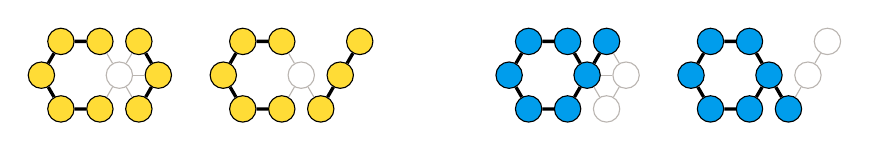
\begin{tikzpicture}[scale=0.33]%{{{
        \begin{scope}[rotate=90]
            \node[draw, circle, fill=uofgsunshine, inner sep=0.5pt, font=\normalsize] (M1) at (90:1.5) {\phantom{0}};
            \node[draw, circle, fill=uofgsunshine, inner sep=0.5pt, font=\normalsize] (M2) at (150:1.5) {\phantom{0}};
            \node[draw, circle, fill=uofgsunshine, inner sep=0.5pt, font=\normalsize] (M3) at (30:1.5) {\phantom{0}};
            \node[draw, circle, fill=uofgsunshine, inner sep=0.5pt, font=\normalsize] (M4) at (210:1.5) {\phantom{0}};
            \node[draw, circle, fill=uofgsunshine, inner sep=0.5pt, font=\normalsize] (M5) at (330:1.5) {\phantom{0}};
            \node[draw, circle, draw=uofgsandstone!40, fill=white, inner sep=0.5pt, font=\normalsize] (M6) at (270:1.5) {\phantom{0}};
            \node[draw, circle, fill=uofgsunshine, inner sep=0.5pt, font=\normalsize] (M7) at ($(210:1.5) + (M6)$) {\phantom{0}};
            \node[draw, circle, fill=uofgsunshine, inner sep=0.5pt, font=\normalsize] (M8) at ($(330:1.5) + (M6)$) {\phantom{0}};
            \node[draw, circle, fill=uofgsunshine, inner sep=0.5pt, font=\normalsize] (M9) at ($(270:1.5) + (M6)$) {\phantom{0}};

            \draw [very thick] (M1) -- (M2);
            \draw [very thick] (M2) -- (M4);
            \draw [very thick] (M3) -- (M5);
            \draw [color=uofgsandstone!40] (M4) -- (M6);
            \draw [color=uofgsandstone!40] (M5) -- (M6);
            \draw [very thick] (M3) -- (M1);
            \draw [color=uofgsandstone!40] (M6) -- (M7);
            \draw [color=uofgsandstone!40] (M6) -- (M8);
            \draw [color=uofgsandstone!40] (M6) -- (M9);
            \draw [very thick] (M7) -- (M9);
            \draw [very thick] (M8) -- (M9);
        \end{scope}

        \begin{scope}[xshift=7cm, rotate=90]
            \node[draw, circle, fill=uofgsunshine, inner sep=0.5pt, font=\normalsize] (M1) at (90:1.5) {\phantom{0}};
            \node[draw, circle, fill=uofgsunshine, inner sep=0.5pt, font=\normalsize] (M2) at (150:1.5) {\phantom{0}};
            \node[draw, circle, fill=uofgsunshine, inner sep=0.5pt, font=\normalsize] (M3) at (30:1.5) {\phantom{0}};
            \node[draw, circle, fill=uofgsunshine, inner sep=0.5pt, font=\normalsize] (M4) at (210:1.5) {\phantom{0}};
            \node[draw, circle, fill=uofgsunshine, inner sep=0.5pt, font=\normalsize] (M5) at (330:1.5) {\phantom{0}};
            \node[draw, circle, draw=uofgsandstone!40, fill=white, inner sep=0.5pt, font=\normalsize] (M6) at (270:1.5) {\phantom{0}};
            \node[draw, circle, fill=uofgsunshine, inner sep=0.5pt, font=\normalsize] (M7) at ($(210:1.5) + (M6)$) {\phantom{0}};
            \node[draw, circle, fill=uofgsunshine, inner sep=0.5pt, font=\normalsize] (M8) at ($(270:1.5) + (M6)$) {\phantom{0}};
            \node[draw, circle, fill=uofgsunshine, inner sep=0.5pt, font=\normalsize] (M9) at ($(330:1.5) + (M8)$) {\phantom{0}};

            \draw [very thick] (M1) -- (M2);
            \draw [very thick] (M2) -- (M4);
            \draw [very thick] (M3) -- (M5);
            \draw [color=uofgsandstone!40] (M4) -- (M6);
            \draw [color=uofgsandstone!40] (M5) -- (M6);
            \draw [very thick] (M3) -- (M1);
            \draw [color=uofgsandstone!40] (M6) -- (M7);
            \draw [very thick] (M7) -- (M8);
            \draw [very thick] (M8) -- (M9);
        \end{scope}

        \begin{scope}[xshift=18cm, rotate=90]
            \node[draw, circle, fill=uofgcobalt, inner sep=0.5pt, font=\normalsize] (M1) at (90:1.5) {\phantom{0}};
            \node[draw, circle, fill=uofgcobalt, inner sep=0.5pt, font=\normalsize] (M2) at (150:1.5) {\phantom{0}};
            \node[draw, circle, fill=uofgcobalt, inner sep=0.5pt, font=\normalsize] (M3) at (30:1.5) {\phantom{0}};
            \node[draw, circle, fill=uofgcobalt, inner sep=0.5pt, font=\normalsize] (M4) at (210:1.5) {\phantom{0}};
            \node[draw, circle, fill=uofgcobalt, inner sep=0.5pt, font=\normalsize] (M5) at (330:1.5) {\phantom{0}};
            \node[draw, circle, fill=uofgcobalt, inner sep=0.5pt, font=\normalsize] (M6) at (270:1.5) {\phantom{0}};
            \node[draw, circle, draw=uofgsandstone!40, fill=white, inner sep=0.5pt, font=\normalsize] (M7) at ($(210:1.5) + (M6)$) {\phantom{0}};
            \node[draw, circle, fill=uofgcobalt, inner sep=0.5pt, font=\normalsize] (M8) at ($(330:1.5) + (M6)$) {\phantom{0}};
            \node[draw, circle, draw=uofgsandstone!40, fill=white, inner sep=0.5pt, font=\normalsize] (M9) at ($(270:1.5) + (M6)$) {\phantom{0}};

            \draw [very thick] (M1) -- (M2);
            \draw [very thick] (M2) -- (M4);
            \draw [very thick] (M3) -- (M5);
            \draw [very thick] (M4) -- (M6);
            \draw [very thick] (M5) -- (M6);
            \draw [very thick] (M3) -- (M1);
            \draw [color=uofgsandstone!40] (M6) -- (M7);
            \draw [very thick] (M6) -- (M8);
            \draw [color=uofgsandstone!40] (M6) -- (M9);
            \draw [color=uofgsandstone!40] (M7) -- (M9);
            \draw [color=uofgsandstone!40] (M8) -- (M9);
        \end{scope}

        \begin{scope}[xshift=25cm, rotate=90]
            \node[draw, circle, fill=uofgcobalt, inner sep=0.5pt, font=\normalsize] (M1) at (90:1.5) {\phantom{0}};
            \node[draw, circle, fill=uofgcobalt, inner sep=0.5pt, font=\normalsize] (M2) at (150:1.5) {\phantom{0}};
            \node[draw, circle, fill=uofgcobalt, inner sep=0.5pt, font=\normalsize] (M3) at (30:1.5) {\phantom{0}};
            \node[draw, circle, fill=uofgcobalt, inner sep=0.5pt, font=\normalsize] (M4) at (210:1.5) {\phantom{0}};
            \node[draw, circle, fill=uofgcobalt, inner sep=0.5pt, font=\normalsize] (M5) at (330:1.5) {\phantom{0}};
            \node[draw, circle, fill=uofgcobalt, inner sep=0.5pt, font=\normalsize] (M6) at (270:1.5) {\phantom{0}};
            \node[draw, circle, fill=uofgcobalt, inner sep=0.5pt, font=\normalsize] (M7) at ($(210:1.5) + (M6)$) {\phantom{0}};
            \node[draw, circle, draw=uofgsandstone!40, fill=white, inner sep=0.5pt, font=\normalsize] (M8) at ($(270:1.5) + (M6)$) {\phantom{0}};
            \node[draw, circle, draw=uofgsandstone!40, fill=white, inner sep=0.5pt, font=\normalsize] (M9) at ($(330:1.5) + (M8)$) {\phantom{0}};

            \draw [very thick] (M1) -- (M2);
            \draw [very thick] (M2) -- (M4);
            \draw [very thick] (M3) -- (M5);
            \draw [very thick] (M4) -- (M6);
            \draw [very thick] (M5) -- (M6);
            \draw [very thick] (M3) -- (M1);
            \draw [very thick] (M6) -- (M7);
            \draw [draw=uofgsandstone!40] (M7) -- (M8);
            \draw [draw=uofgsandstone!40] (M8) -- (M9);
        \end{scope}
\end{tikzpicture}
\caption{A maximum common induced subgraph of the first two graphs has eight vertices, shaded.
However, if we require the common subgraph to be connected, only seven vertices may be
selected---one way to do this is shown in the third and fourth graphs.}\label{figure:mcsexample}
\end{figure}

Maximum common subgraph problems arise in biology and chemistry
\cite{DBLP:journals/jcamd/RaymondW02a,Ehrlich:2011}, in computer vision
\cite{DBLP:journals/jair/CookH94}, in the analysis of source code
\cite{DBLP:journals/tkde/DjokoCH97}, binary programs \cite{DBLP:conf/icics/GaoRS08}, and circuit
designs \cite{DBLP:journals/jair/CookH94}, in character recognition problems \cite{SIWEILU1991617},
and in many other domains \cite{Shasha:2002:AAT:543613.543620}, both directly and as a way of
measuring the similarity or difference between two graphs
\cite{DBLP:journals/prl/Bunke97,DBLP:journals/prl/FernandezV01,KriegeThesis}.


\paragraph{Definition of the Maximum Common (Connected) Subgraph Problem.}
We introduce definitions and algorithms on undirected and unlabelled graphs. The extension to directed or labelled graphs is straightforward and discussed in Section \ref{extension}. An undirected graph $G$ is defined by a finite set of nodes $N_G$ and a set of edges $E_G\subseteq N_G\times N_G$ such that each edge is an undirected pair of nodes.

Given a graph $G$, two nodes $n_s, n_e \in N_G$ are connected by a path in $G$ if there exists a sequence of nodes $<n_0,\ldots n_k>$ such that $n_0=n_s$, $n_k=n_e$ and each couple of successive nodes is connected by an edge, {\em i.e.}, $\forall i\in [1,k], \{n_{i-1},n_i\}\in E_G$. A graph $G$ is \emph{connected} if every pair of nodes is connected by a path.

A graph $G$ is \emph{isomorphic} to another graph $G'$ if there exists a bijective function $f:N_G\rightarrow N_{G'}$ which preserves edges, \emph{i.e.}, $\forall (u,v)\in N_G\times N_G, \{u,v\}\in E_G\Leftrightarrow \{f(u),f(v)\}\in E_{G'}$.

A {\em subgraph} is obtained by removing nodes, and all their incident edges, {\em i.e.}, $G'$ is a \emph{subgraph} of $G$ if $N_{G'}\subseteq N_G$ and $E_{G'}=E_G\cap(N_{G'}\times N_{G'})$.
In this definition, we only remove edges incident to removed nodes. This is usually called induced subgraph in the litterature. We may also allow to remove edges which are not incident to removed nodes, thus leading to partial subgraphs. In this paper, we only consider induced subgraphs. However, all algorithms may be extended to the partial case, as explained in \cite{DBLP:conf/cp/NdiayeS11}.

A \emph{common subgraph} of two graphs $G$ and $G'$ is a graph isomorphic to subgraphs of $G$ and $G'$. A \emph{common connected subgraph} is a common subgraph which is connected.
A \emph{Maximum Common Subgraph} (MCS) (resp. \emph{Maximum Common Connected Subgraph} (MCCS) is a common subgraph (resp. common connected subgraph) which has a maximum number of nodes. Examples of MCS and MCCS are given in Fig. \ref{figure:mcsexample}.

\paragraph{Overview of the paper.} In Section \ref{existing}, we review existing approaches for solving the MCS problem, with a specific focus on Constraint Programming (CP)-based approaches and on clique-based approaches that reduce the problem to finding a maximum clique in an association graph. 

Conventional wisdom is that clique-based approaches are less effective in practice, but previous experimental evaluations have used weak clique algorithms, or even maximal clique enumeration algorithms. 
Therefore, in Section \ref{eval1}, we  re-evaluate the clique-based approach using a modern algorithm, and we show that it outperforms CP on labelled graphs, and that it is competitive with CP on non labelled graphs. 

Then, in Section \ref{mccs}, we consider the MCCS problem. For the CP approach, we may add a global connectedness constraint to the model. Alternatively, we may use a special branching rule to grow connected subgraphs only, as proposed in \cite{DBLP:conf/mco/VismaraV08}. These two techniques may be combined, and we experimentally show that the best results are obtained when combining them. 
When solving the MCCS problem with a clique-based approach, neither technique seems directly viable with an association graph encoding.
However, we show that it is possible to adapt the combined branching and bounding rule used by modern clique algorithms to preserve connectedness during search.
We compare the clique-based approach with the best CP variant for the MCCS, and we show that it outperforms CP on non labelled graphs, whereas it is outperformed by CP on labelled graphs.


\section{Existing Complete Approaches for MCS}\label{existing}


There exist two main approaches for solving MCS: The first approach (described in \ref{CP}) is based on CP; The second approach (described in \ref{clique}) is based on a reformulation of MCS into a maximum clique problem. Both approaches are described for non directed and non labelled graphs. Their extension to directed or labelled graphs is discussed in Section \ref{extension}

\subsection{CP model for MCS}
\label{CP}

McGregor \cite{McGreg82} proposed a Branch \& Bound approach: Each branch of the search tree corresponds to the matching of two nodes, and a  bounding function evaluates the number of nodes that still may be matched so that the current branch is pruned as soon as this bound becomes lower than the size of the largest known common subgraph. CP approaches may be viewed as enhancements of this Branch \& Bound approach. 

Vismara and Valery  \cite{DBLP:conf/mco/VismaraV08} introduced a first CP model. Given two graphs $G$ and $G'$, this model associates a variable $x_u$ with every node $u$ of $G$, and the domain of this variable contains all nodes of $G'$, plus an additional value $\bot$: variable $x_u$ is assigned to $\bot$ if node $u$ is not matched to any node of $G'$; otherwise $x_u$ is assigned to the node of $G'$ it is matched with. Edge constraints are introduced in order to ensure that variable assignments preserve edges between matched nodes, {\em i.e.}, 
$\forall \{u,v\}\subseteq N_G, (x_u=\bot)\vee (x_v=\bot) \vee (\{u,v\}\in E_G\Leftrightarrow \{x_u,x_v\}\in E_{G'})$. Difference constraints are introduced in order to ensure that each node of $G'$ is assigned to at most one variable, {\em i.e.}, $\forall \{u,v\}\subseteq N_G, (x_u=\bot)\vee (x_v=\bot) \vee (x_u\neq x_v)$.

This CP model is improved in \cite{DBLP:conf/cp/NdiayeS11} by replacing binary difference constraints with a soft global allDifferent constraint which maximizes the number of $x_u$ variables that are assigned to values different from $\bot$, while ensuring they are all different when they are not assigned to $\bot$.
Different constraint propagation techniques are compared in \cite{DBLP:conf/cp/NdiayeS11}. The combination ``MAC+Bound'' (resp. ``FC+Bound'') obtains the best results on labelled (resp. non labelled) graphs and outperforms the approach of \cite{McGreg82} and the CP model of \cite{DBLP:conf/mco/VismaraV08}. The combination ``MAC+Bound'' maintains arc consistency~\cite{sabi94} of edge constraints, whereas the conbination ``FC+Bound'' simply performs forward-checking on these constraints. In both combinations, the ``Bound'' filtering checks whether it is possible to assign distinct values to enough $x_u$ variables to surpass the best cost found so far (it is a weaker version of GAC(\emph{softAllDiff}) \cite{peti01} which computes the maximum number of variables that can be assigned distinct values).



\subsection{Reformulation of MCS as a maximum clique problem}
\label{clique}

We may solve MCS by introducing an association graph and searching for a maximum clique in it \cite{bala86,dura99,DBLP:journals/jcamd/RaymondW02a}.

An association graph of two graphs $G$ and $G'$ is an undirected graph $A_{G,G'}$ whose set of nodes is $N_{A_{G,G'}} = N_G \times N_{G'}$. To avoid confusing nodes of $A_{G,G'}$ with initial graph nodes, nodes of $A_{G,G'}$ are called matching nodes, as each node $(u,u')$ of $A_{G,G'}$ denotes the matching of $u$ with $u'$. Edges of $A_{G,G'}$ connect matching nodes which are compatible, {\em i.e.}, $E_{A_{G,G'}} = \big\{\{(u,u'),(v,v')\}\subseteq N_{A_{G,G'}}$, $(u,u')$ and $(v,v')$ are compatible$\big\}$, where two matching nodes $(u,u')$ and $(v,v')$ of $N_{A_{G,G'}}$ are compatible if $u \neq v$ and $u' \neq v'$, and if they preserve edges (\emph{i.e.}, $\{u,v\} \in E_G \Leftrightarrow \{u',v'\} \in E_{G'}$).

A \emph{clique} is a subgraph whose nodes are all linked pairwise.
A clique is \emph{maximal} if it is not strictly included in any other clique, and it is \emph{maximum} if it is the largest clique of a given graph, with respect to the number of nodes.

A clique in $A_{G,G'}$ corresponds to a set of compatible matchings. Therefore, such a clique corresponds to a common subgraph, and a maximum clique of $A_{G,G'}$ is a MCS of $G$ and $G'$.
It follows that any method able to find a maximum clique in a graph can be used to solve the MCS problem. 

Note that the association graph is a partial subgraph of the microstructure \cite{DBLP:conf/aaai/Jegou93a} associated with the CP model of  \cite{DBLP:conf/mco/VismaraV08}: The microstructure has more matching nodes than the association graph because it has a matching node $(u,\bot)$ for each node $u$ of $G$. Each clique of size $|N_G|$ in the microstructure corresponds to a common subgraph the size of which is defined by the number of nodes that do not contain $\bot$.


\subsection{Extension to Labeled or Directed Graphs}\label{extension}

In some applications, nodes and edges are associated with labels. We note $\lambda(u)$ and $\lambda(\{u,v\})$ the label of a node $u$ and an edge $\{u,v\}$, respectively. In this case, the common  subgraph must match components the labels of which are compatible, and we note $\simeq$ the compatibility relationship, {\em i.e.}, labels $\lambda_1$ and $\lambda_2$ are compatible if $\lambda_1\simeq\lambda_2$. This kind of label compatibility constraint is handled in a straightforward way in both CP and clique-based approaches:
\begin{itemize}
\item For CP, we restrict the domain of every variable $x_u$ to nodes with compatible labels, {\em i.e.}, $\forall u\in N_G, D(x_u) = \{\bot\}\cup \{u'\in N_{G'}, \lambda(u)\simeq\lambda(u')\}$. We also have to ensure that edge labels are preserved in edge constraints, {\em i.e.}, $\forall \{u,v\}\subseteq N_G, (x_u=\bot)\vee (x_v=\bot) \vee ((\{u,v\}\in E_G\Leftrightarrow \{x_u,x_v\}\in E_{G'}) \wedge (\lambda(\{u,v\}) \simeq \lambda(\{x_u,x_v\})))$.

\item For clique-based approaches, label compatibility is handled through the definition of the association graph, by restricting the set of matching nodes to pairs of nodes with compatible labels, {\em i.e.}, $N_{G_C} = \{(u,u')\in N_G\times N_{G'}, \lambda(u)\simeq\lambda(u')\}$. Also, edges of the association graph are restricted to pairs $\{(u,u'),(v,v')\}$ such that $\lambda(\{u,v\}) \simeq \lambda(\{u',v')\}$.
\end{itemize} 
Labels usually simplify the solution process, both for CP and clique-based approaches: Node labels reduce domain sizes for CP, and the number of matching nodes in the association graphs; Edge labels tighten edge constraints for CP, and make the association graph sparser for clique-based approaches. 

The extension of MCS algorithms to directed graphs is straightforward: For CP, edge orientation is handled in edge constraints; for clique-based approaches, it is handled in the definition of the association graph edges. In both cases, adding orientations to edges usually simplifies the problem: It tightens edge constraints for CP, and it makes the association graph sparser for  clique-based approaches.


\section{Re-Evaluating the Clique Model}\label{eval1}



Previous experimental work has used a maximal clique enumeration algorithm, even for the
maximisation problem. ?? check this! I recall someone using a bad max clique algorithm too.
\cite{DBLP:conf/sspr/BunkeFGSV02,DBLP:journals/jgaa/ConteFV07}

We instead use a maximum clique algorithm.

Also sparse stuff, but association graphs aren't sparse enough.

Say which clique algorithm we're using.


\subsection{Datasets}

We consider a randomly generated database described in \cite{DBLP:journals/prl/SantoFSV03,DBLP:journals/jgaa/ConteFV07}. 
The dataset contains different classes of graphs: Randomly connected graphs with connectivity $\eta\in\{0.05,0.2\}$ (r005 and r02); 2D, 3D, and 4D regular meshes (m2D, m3D, m4D); 2D, 3D, and 4D irregular meshes with $\rho=0.6$ (m2Dr, m3Dr, and m4Dr); regular bounded valence graphs with $V\in\{3,9\}$ (b03 and b09) and irregular bounded valence graphs with $V\in\{3,9\}$ (b03m and b09m). Each class contains XXX pairs of graphs: YYY for each of the 5 possible sizes of the MCIS ({\em i.e.}, 10\%, 30\%, 50\%, 70\% and 90\% of the number of nodes of the original graphs). 

For each pair of graphs, there are 3 different labelings such that the number of different labels is equal to 33\%, 50\% or 75\% of the number of nodes. In this paper, we report experiments with non labelled graphs (labels are ignored), and with 33\% labellings.


\subsection{Experimental Evaluation}

\begin{figure}[p]
    \centering
    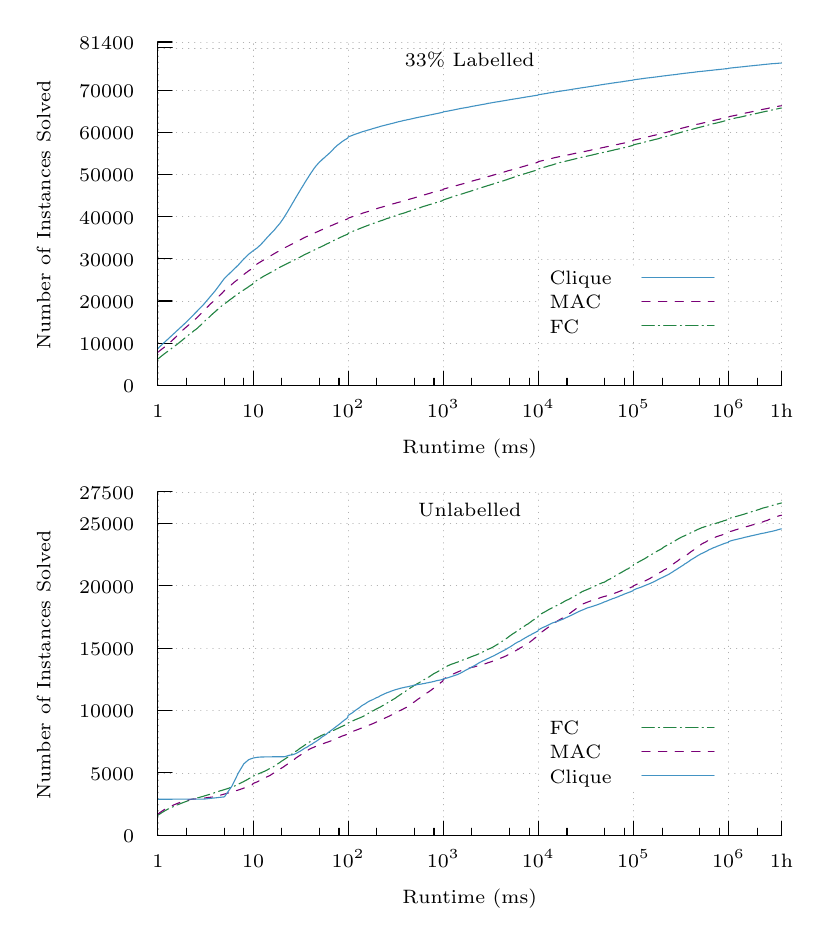
\begin{tikzpicture}[gnuplot]
%% generated with GNUPLOT 5.0p0 (Lua 5.2; terminal rev. 99, script rev. 100)
%% Tue 19 Apr 2016 13:36:59 AEST
\tikzset{every node/.append style={font={\scriptsize}}}
% \path (0.000,0.000) rectangle (10.160,11.430);
\gpcolor{color=gp lt color axes}
\gpsetlinetype{gp lt axes}
\gpsetdashtype{gp dt axes}
\gpsetlinewidth{0.50}
\draw[gp path] (1.688,10.986)--(9.607,10.986);
\gpcolor{color=gp lt color border}
\gpsetlinetype{gp lt border}
\gpsetdashtype{gp dt solid}
\gpsetlinewidth{1.00}
\draw[gp path] (1.688,10.986)--(1.868,10.986);
\gpcolor{color=gp lt color axes}
\gpsetlinetype{gp lt axes}
\gpsetdashtype{gp dt axes}
\gpsetlinewidth{0.50}
\draw[gp path] (1.688,11.061)--(9.607,11.061);
\gpcolor{color=gp lt color border}
\gpsetlinetype{gp lt border}
\gpsetdashtype{gp dt solid}
\gpsetlinewidth{1.00}
\draw[gp path] (1.688,11.061)--(1.868,11.061);
\node[gp node right] at (1.504,11.061) {81400};
\gpcolor{color=gp lt color axes}
\gpsetlinetype{gp lt axes}
\gpsetdashtype{gp dt axes}
\gpsetlinewidth{0.50}
\draw[gp path] (1.688,6.700)--(9.607,6.700);
\gpcolor{color=gp lt color border}
\gpsetlinetype{gp lt border}
\gpsetdashtype{gp dt solid}
\gpsetlinewidth{1.00}
\draw[gp path] (1.688,6.700)--(1.868,6.700);
\node[gp node right] at (1.504,6.700) {$0$};
\gpcolor{color=gp lt color axes}
\gpsetlinetype{gp lt axes}
\gpsetdashtype{gp dt axes}
\gpsetlinewidth{0.50}
\draw[gp path] (1.688,7.236)--(9.607,7.236);
\gpcolor{color=gp lt color border}
\gpsetlinetype{gp lt border}
\gpsetdashtype{gp dt solid}
\gpsetlinewidth{1.00}
\draw[gp path] (1.688,7.236)--(1.868,7.236);
\node[gp node right] at (1.504,7.236) {$10000$};
\gpcolor{color=gp lt color axes}
\gpsetlinetype{gp lt axes}
\gpsetdashtype{gp dt axes}
\gpsetlinewidth{0.50}
\draw[gp path] (1.688,7.771)--(6.546,7.771);
\draw[gp path] (8.934,7.771)--(9.607,7.771);
\gpcolor{color=gp lt color border}
\gpsetlinetype{gp lt border}
\gpsetdashtype{gp dt solid}
\gpsetlinewidth{1.00}
\draw[gp path] (1.688,7.771)--(1.868,7.771);
\node[gp node right] at (1.504,7.771) {$20000$};
\gpcolor{color=gp lt color axes}
\gpsetlinetype{gp lt axes}
\gpsetdashtype{gp dt axes}
\gpsetlinewidth{0.50}
\draw[gp path] (1.688,8.307)--(9.607,8.307);
\gpcolor{color=gp lt color border}
\gpsetlinetype{gp lt border}
\gpsetdashtype{gp dt solid}
\gpsetlinewidth{1.00}
\draw[gp path] (1.688,8.307)--(1.868,8.307);
\node[gp node right] at (1.504,8.307) {$30000$};
\gpcolor{color=gp lt color axes}
\gpsetlinetype{gp lt axes}
\gpsetdashtype{gp dt axes}
\gpsetlinewidth{0.50}
\draw[gp path] (1.688,8.843)--(9.607,8.843);
\gpcolor{color=gp lt color border}
\gpsetlinetype{gp lt border}
\gpsetdashtype{gp dt solid}
\gpsetlinewidth{1.00}
\draw[gp path] (1.688,8.843)--(1.868,8.843);
\node[gp node right] at (1.504,8.843) {$40000$};
\gpcolor{color=gp lt color axes}
\gpsetlinetype{gp lt axes}
\gpsetdashtype{gp dt axes}
\gpsetlinewidth{0.50}
\draw[gp path] (1.688,9.379)--(9.607,9.379);
\gpcolor{color=gp lt color border}
\gpsetlinetype{gp lt border}
\gpsetdashtype{gp dt solid}
\gpsetlinewidth{1.00}
\draw[gp path] (1.688,9.379)--(1.868,9.379);
\node[gp node right] at (1.504,9.379) {$50000$};
\gpcolor{color=gp lt color axes}
\gpsetlinetype{gp lt axes}
\gpsetdashtype{gp dt axes}
\gpsetlinewidth{0.50}
\draw[gp path] (1.688,9.914)--(9.607,9.914);
\gpcolor{color=gp lt color border}
\gpsetlinetype{gp lt border}
\gpsetdashtype{gp dt solid}
\gpsetlinewidth{1.00}
\draw[gp path] (1.688,9.914)--(1.868,9.914);
\node[gp node right] at (1.504,9.914) {$60000$};
\gpcolor{color=gp lt color axes}
\gpsetlinetype{gp lt axes}
\gpsetdashtype{gp dt axes}
\gpsetlinewidth{0.50}
\draw[gp path] (1.688,10.450)--(9.607,10.450);
\gpcolor{color=gp lt color border}
\gpsetlinetype{gp lt border}
\gpsetdashtype{gp dt solid}
\gpsetlinewidth{1.00}
\draw[gp path] (1.688,10.450)--(1.868,10.450);
\node[gp node right] at (1.504,10.450) {$70000$};
\gpcolor{color=gp lt color axes}
\gpsetlinetype{gp lt axes}
\gpsetdashtype{gp dt axes}
\gpsetlinewidth{0.50}
\draw[gp path] (1.688,10.986)--(9.607,10.986);
\gpcolor{color=gp lt color border}
\gpsetlinetype{gp lt border}
\gpsetdashtype{gp dt solid}
\gpsetlinewidth{1.00}
\draw[gp path] (1.688,10.986)--(1.868,10.986);
\gpcolor{color=gp lt color axes}
\gpsetlinetype{gp lt axes}
\gpsetdashtype{gp dt axes}
\gpsetlinewidth{0.50}
\draw[gp path] (1.688,6.700)--(1.688,11.061);
\gpcolor{color=gp lt color border}
\gpsetlinetype{gp lt border}
\gpsetdashtype{gp dt solid}
\gpsetlinewidth{1.00}
\draw[gp path] (1.688,6.700)--(1.688,6.880);
\node[gp node center] at (1.688,6.392) {1};
\gpcolor{color=gp lt color axes}
\gpsetlinetype{gp lt axes}
\gpsetdashtype{gp dt axes}
\gpsetlinewidth{0.50}
\draw[gp path] (2.896,6.700)--(2.896,11.061);
\gpcolor{color=gp lt color border}
\gpsetlinetype{gp lt border}
\gpsetdashtype{gp dt solid}
\gpsetlinewidth{1.00}
\draw[gp path] (2.896,6.700)--(2.896,6.880);
\node[gp node center] at (2.896,6.392) {10};
\gpcolor{color=gp lt color axes}
\gpsetlinetype{gp lt axes}
\gpsetdashtype{gp dt axes}
\gpsetlinewidth{0.50}
\draw[gp path] (9.607,6.700)--(9.607,11.061);
\gpcolor{color=gp lt color border}
\gpsetlinetype{gp lt border}
\gpsetdashtype{gp dt solid}
\gpsetlinewidth{1.00}
\draw[gp path] (9.607,6.700)--(9.607,6.880);
\node[gp node center] at (9.607,6.392) {1h};
\gpcolor{color=gp lt color axes}
\gpsetlinetype{gp lt axes}
\gpsetdashtype{gp dt axes}
\gpsetlinewidth{0.50}
\draw[gp path] (1.688,6.700)--(1.688,11.061);
\gpcolor{color=gp lt color border}
\gpsetlinetype{gp lt border}
\gpsetdashtype{gp dt solid}
\gpsetlinewidth{1.00}
\draw[gp path] (1.688,6.700)--(1.688,6.880);
\draw[gp path] (2.052,6.700)--(2.052,6.790);
\draw[gp path] (2.532,6.700)--(2.532,6.790);
\draw[gp path] (2.779,6.700)--(2.779,6.790);
\gpcolor{color=gp lt color axes}
\gpsetlinetype{gp lt axes}
\gpsetdashtype{gp dt axes}
\gpsetlinewidth{0.50}
\draw[gp path] (2.896,6.700)--(2.896,11.061);
\gpcolor{color=gp lt color border}
\gpsetlinetype{gp lt border}
\gpsetdashtype{gp dt solid}
\gpsetlinewidth{1.00}
\draw[gp path] (2.896,6.700)--(2.896,6.880);
\draw[gp path] (3.259,6.700)--(3.259,6.790);
\draw[gp path] (3.740,6.700)--(3.740,6.790);
\draw[gp path] (3.987,6.700)--(3.987,6.790);
\gpcolor{color=gp lt color axes}
\gpsetlinetype{gp lt axes}
\gpsetdashtype{gp dt axes}
\gpsetlinewidth{0.50}
\draw[gp path] (4.104,6.700)--(4.104,11.061);
\gpcolor{color=gp lt color border}
\gpsetlinetype{gp lt border}
\gpsetdashtype{gp dt solid}
\gpsetlinewidth{1.00}
\draw[gp path] (4.104,6.700)--(4.104,6.880);
\node[gp node center] at (4.104,6.392) {$10^{2}$};
\draw[gp path] (4.467,6.700)--(4.467,6.790);
\draw[gp path] (4.948,6.700)--(4.948,6.790);
\draw[gp path] (5.194,6.700)--(5.194,6.790);
\gpcolor{color=gp lt color axes}
\gpsetlinetype{gp lt axes}
\gpsetdashtype{gp dt axes}
\gpsetlinewidth{0.50}
\draw[gp path] (5.312,6.700)--(5.312,11.061);
\gpcolor{color=gp lt color border}
\gpsetlinetype{gp lt border}
\gpsetdashtype{gp dt solid}
\gpsetlinewidth{1.00}
\draw[gp path] (5.312,6.700)--(5.312,6.880);
\node[gp node center] at (5.312,6.392) {$10^{3}$};
\draw[gp path] (5.675,6.700)--(5.675,6.790);
\draw[gp path] (6.156,6.700)--(6.156,6.790);
\draw[gp path] (6.402,6.700)--(6.402,6.790);
\gpcolor{color=gp lt color axes}
\gpsetlinetype{gp lt axes}
\gpsetdashtype{gp dt axes}
\gpsetlinewidth{0.50}
\draw[gp path] (6.519,6.700)--(6.519,11.061);
\gpcolor{color=gp lt color border}
\gpsetlinetype{gp lt border}
\gpsetdashtype{gp dt solid}
\gpsetlinewidth{1.00}
\draw[gp path] (6.519,6.700)--(6.519,6.880);
\node[gp node center] at (6.519,6.392) {$10^{4}$};
\draw[gp path] (6.883,6.700)--(6.883,6.790);
\draw[gp path] (7.364,6.700)--(7.364,6.790);
\draw[gp path] (7.610,6.700)--(7.610,6.790);
\gpcolor{color=gp lt color axes}
\gpsetlinetype{gp lt axes}
\gpsetdashtype{gp dt axes}
\gpsetlinewidth{0.50}
\draw[gp path] (7.727,6.700)--(7.727,7.302);
\draw[gp path] (7.727,8.226)--(7.727,11.061);
\gpcolor{color=gp lt color border}
\gpsetlinetype{gp lt border}
\gpsetdashtype{gp dt solid}
\gpsetlinewidth{1.00}
\draw[gp path] (7.727,6.700)--(7.727,6.880);
\node[gp node center] at (7.727,6.392) {$10^{5}$};
\draw[gp path] (8.091,6.700)--(8.091,6.790);
\draw[gp path] (8.571,6.700)--(8.571,6.790);
\draw[gp path] (8.818,6.700)--(8.818,6.790);
\gpcolor{color=gp lt color axes}
\gpsetlinetype{gp lt axes}
\gpsetdashtype{gp dt axes}
\gpsetlinewidth{0.50}
\draw[gp path] (8.935,6.700)--(8.935,11.061);
\gpcolor{color=gp lt color border}
\gpsetlinetype{gp lt border}
\gpsetdashtype{gp dt solid}
\gpsetlinewidth{1.00}
\draw[gp path] (8.935,6.700)--(8.935,6.880);
\node[gp node center] at (8.935,6.392) {$10^{6}$};
\draw[gp path] (9.299,6.700)--(9.299,6.790);
\draw[gp path] (1.688,11.061)--(1.688,6.700)--(9.607,6.700);
\node[gp node center,rotate=-270] at (0.246,8.880) {Number of Instances Solved};
\node[gp node center] at (5.647,5.930) {Runtime (ms)};
\node[gp node left] at (6.546,8.072) {Clique};
\gpcolor{rgb color={0.263,0.576,0.765}}
\draw[gp path] (7.834,8.072)--(8.750,8.072);
\draw[gp path] (1.688,7.170)--(2.052,7.507)--(2.264,7.723)--(2.415,7.901)--(2.532,8.058)%
  --(2.628,8.151)--(2.709,8.229)--(2.779,8.306)--(2.841,8.366)--(2.896,8.409)--(2.946,8.444)%
  --(2.991,8.485)--(3.033,8.530)--(3.072,8.574)--(3.109,8.614)--(3.142,8.648)--(3.174,8.682)%
  --(3.204,8.720)--(3.233,8.752)--(3.259,8.789)--(3.285,8.826)--(3.309,8.865)--(3.333,8.903)%
  --(3.355,8.941)--(3.376,8.976)--(3.397,9.013)--(3.417,9.046)--(3.436,9.080)--(3.454,9.110)%
  --(3.472,9.140)--(3.489,9.168)--(3.506,9.197)--(3.522,9.222)--(3.538,9.248)--(3.553,9.274)%
  --(3.568,9.298)--(3.582,9.320)--(3.596,9.341)--(3.610,9.364)--(3.623,9.385)--(3.636,9.404)%
  --(3.649,9.422)--(3.661,9.441)--(3.673,9.458)--(3.685,9.473)--(3.696,9.487)--(3.708,9.501)%
  --(3.719,9.513)--(3.729,9.524)--(3.740,9.537)--(3.750,9.546)--(3.761,9.555)--(3.771,9.565)%
  --(3.780,9.574)--(3.790,9.582)--(3.800,9.590)--(3.809,9.598)--(3.818,9.606)--(3.827,9.615)%
  --(3.836,9.622)--(3.844,9.630)--(3.853,9.637)--(3.861,9.645)--(3.870,9.653)--(3.878,9.661)%
  --(3.886,9.668)--(3.894,9.676)--(3.901,9.684)--(3.909,9.692)--(3.917,9.701)--(3.924,9.710)%
  --(3.931,9.716)--(3.939,9.724)--(3.946,9.730)--(3.953,9.736)--(3.960,9.744)--(3.967,9.749)%
  --(3.973,9.754)--(3.980,9.759)--(3.987,9.764)--(3.993,9.769)--(4.000,9.774)--(4.006,9.779)%
  --(4.012,9.783)--(4.018,9.789)--(4.025,9.794)--(4.031,9.798)--(4.037,9.802)--(4.043,9.806)%
  --(4.048,9.809)--(4.054,9.813)--(4.060,9.817)--(4.066,9.821)--(4.071,9.823)--(4.077,9.827)%
  --(4.082,9.830)--(4.088,9.834)--(4.093,9.837)--(4.098,9.840)--(4.104,9.855)--(4.154,9.874)%
  --(4.199,9.892)--(4.241,9.905)--(4.280,9.920)--(4.316,9.930)--(4.350,9.941)--(4.382,9.949)%
  --(4.412,9.959)--(4.440,9.967)--(4.467,9.976)--(4.493,9.982)--(4.517,9.990)--(4.541,9.996)%
  --(4.563,10.002)--(4.584,10.007)--(4.605,10.013)--(4.625,10.017)--(4.644,10.023)--(4.662,10.026)%
  --(4.680,10.031)--(4.697,10.036)--(4.714,10.041)--(4.730,10.044)--(4.746,10.049)--(4.761,10.052)%
  --(4.776,10.055)--(4.790,10.059)--(4.804,10.063)--(4.818,10.066)--(4.831,10.068)--(4.844,10.070)%
  --(4.856,10.074)--(4.869,10.076)--(4.881,10.078)--(4.893,10.081)--(4.904,10.084)--(4.915,10.086)%
  --(4.927,10.089)--(4.937,10.091)--(4.948,10.094)--(4.958,10.096)--(4.969,10.099)--(4.979,10.100)%
  --(4.988,10.103)--(4.998,10.105)--(5.007,10.107)--(5.017,10.108)--(5.026,10.111)--(5.035,10.112)%
  --(5.044,10.114)--(5.052,10.115)--(5.061,10.117)--(5.069,10.118)--(5.077,10.121)--(5.086,10.122)%
  --(5.094,10.124)--(5.101,10.126)--(5.109,10.127)--(5.117,10.128)--(5.124,10.130)--(5.132,10.132)%
  --(5.139,10.134)--(5.146,10.135)--(5.154,10.136)--(5.161,10.137)--(5.168,10.139)--(5.174,10.140)%
  --(5.181,10.142)--(5.188,10.143)--(5.194,10.145)--(5.201,10.146)--(5.207,10.147)--(5.214,10.148)%
  --(5.220,10.150)--(5.226,10.151)--(5.232,10.152)--(5.238,10.153)--(5.244,10.155)--(5.250,10.156)%
  --(5.256,10.158)--(5.262,10.159)--(5.268,10.160)--(5.273,10.161)--(5.279,10.163)--(5.285,10.164)%
  --(5.290,10.165)--(5.296,10.166)--(5.301,10.167)--(5.306,10.168)--(5.312,10.174)--(5.362,10.182)%
  --(5.407,10.191)--(5.449,10.199)--(5.488,10.207)--(5.524,10.215)--(5.558,10.221)--(5.590,10.226)%
  --(5.620,10.231)--(5.648,10.237)--(5.675,10.243)--(5.701,10.247)--(5.725,10.252)--(5.748,10.256)%
  --(5.771,10.260)--(5.792,10.264)--(5.813,10.268)--(5.833,10.271)--(5.852,10.275)--(5.870,10.279)%
  --(5.888,10.283)--(5.905,10.285)--(5.922,10.288)--(5.938,10.291)--(5.953,10.294)--(5.969,10.296)%
  --(5.983,10.299)--(5.998,10.301)--(6.012,10.303)--(6.025,10.305)--(6.039,10.308)--(6.052,10.310)%
  --(6.064,10.312)--(6.077,10.314)--(6.089,10.316)--(6.101,10.318)--(6.112,10.320)--(6.123,10.322)%
  --(6.134,10.324)--(6.145,10.326)--(6.156,10.328)--(6.166,10.330)--(6.176,10.331)--(6.186,10.333)%
  --(6.196,10.334)--(6.206,10.336)--(6.215,10.338)--(6.225,10.339)--(6.234,10.341)--(6.243,10.342)%
  --(6.251,10.343)--(6.260,10.344)--(6.269,10.346)--(6.277,10.347)--(6.285,10.349)--(6.293,10.350)%
  --(6.301,10.351)--(6.309,10.353)--(6.317,10.354)--(6.325,10.355)--(6.332,10.356)--(6.340,10.358)%
  --(6.347,10.359)--(6.354,10.360)--(6.361,10.362)--(6.368,10.363)--(6.375,10.364)--(6.382,10.365)%
  --(6.389,10.366)--(6.396,10.367)--(6.402,10.368)--(6.409,10.369)--(6.415,10.370)--(6.422,10.371)%
  --(6.428,10.372)--(6.434,10.373)--(6.440,10.374)--(6.446,10.375)--(6.452,10.376)--(6.458,10.377)%
  --(6.464,10.378)--(6.470,10.379)--(6.476,10.380)--(6.481,10.381)--(6.487,10.381)--(6.492,10.383)%
  --(6.498,10.383)--(6.503,10.384)--(6.509,10.385)--(6.514,10.386)--(6.519,10.391)--(6.569,10.399)%
  --(6.615,10.406)--(6.657,10.414)--(6.696,10.420)--(6.732,10.426)--(6.766,10.432)--(6.798,10.436)%
  --(6.828,10.441)--(6.856,10.445)--(6.883,10.449)--(6.909,10.453)--(6.933,10.457)--(6.956,10.461)%
  --(6.979,10.465)--(7.000,10.468)--(7.021,10.471)--(7.040,10.474)--(7.059,10.478)--(7.078,10.480)%
  --(7.096,10.483)--(7.113,10.485)--(7.130,10.488)--(7.146,10.490)--(7.161,10.493)--(7.177,10.495)%
  --(7.191,10.498)--(7.206,10.499)--(7.220,10.502)--(7.233,10.504)--(7.247,10.506)--(7.260,10.508)%
  --(7.272,10.510)--(7.285,10.512)--(7.297,10.514)--(7.308,10.516)--(7.320,10.518)--(7.331,10.520)%
  --(7.342,10.521)--(7.353,10.523)--(7.364,10.525)--(7.374,10.526)--(7.384,10.528)--(7.394,10.529)%
  --(7.404,10.530)--(7.414,10.532)--(7.423,10.534)--(7.432,10.535)--(7.441,10.536)--(7.450,10.538)%
  --(7.459,10.539)--(7.468,10.540)--(7.476,10.541)--(7.485,10.543)--(7.493,10.544)--(7.501,10.545)%
  --(7.509,10.546)--(7.517,10.547)--(7.525,10.548)--(7.533,10.550)--(7.540,10.551)--(7.548,10.551)%
  --(7.555,10.552)--(7.562,10.553)--(7.569,10.554)--(7.576,10.555)--(7.583,10.556)--(7.590,10.557)%
  --(7.597,10.559)--(7.604,10.560)--(7.610,10.561)--(7.617,10.562)--(7.623,10.563)--(7.629,10.564)%
  --(7.636,10.565)--(7.642,10.566)--(7.648,10.566)--(7.654,10.567)--(7.660,10.568)--(7.666,10.569)%
  --(7.672,10.570)--(7.678,10.571)--(7.683,10.572)--(7.689,10.573)--(7.695,10.573)--(7.700,10.574)%
  --(7.706,10.574)--(7.711,10.575)--(7.717,10.576)--(7.722,10.577)--(7.727,10.580)--(7.777,10.587)%
  --(7.823,10.593)--(7.865,10.599)--(7.904,10.604)--(7.940,10.608)--(7.974,10.612)--(8.006,10.616)%
  --(8.036,10.620)--(8.064,10.624)--(8.091,10.627)--(8.116,10.631)--(8.141,10.633)--(8.164,10.637)%
  --(8.186,10.639)--(8.208,10.642)--(8.228,10.644)--(8.248,10.646)--(8.267,10.648)--(8.286,10.651)%
  --(8.304,10.654)--(8.321,10.656)--(8.337,10.658)--(8.354,10.660)--(8.369,10.662)--(8.384,10.664)%
  --(8.399,10.666)--(8.414,10.667)--(8.428,10.669)--(8.441,10.671)--(8.454,10.672)--(8.467,10.673)%
  --(8.480,10.675)--(8.492,10.676)--(8.504,10.678)--(8.516,10.680)--(8.528,10.681)--(8.539,10.683)%
  --(8.550,10.684)--(8.561,10.685)--(8.571,10.686)--(8.582,10.688)--(8.592,10.688)--(8.602,10.689)%
  --(8.612,10.690)--(8.621,10.691)--(8.631,10.692)--(8.640,10.693)--(8.649,10.694)--(8.658,10.695)%
  --(8.667,10.696)--(8.676,10.697)--(8.684,10.698)--(8.693,10.699)--(8.701,10.700)--(8.709,10.700)%
  --(8.717,10.701)--(8.725,10.702)--(8.733,10.703)--(8.740,10.704)--(8.748,10.705)--(8.755,10.706)%
  --(8.763,10.706)--(8.770,10.707)--(8.777,10.708)--(8.784,10.709)--(8.791,10.709)--(8.798,10.710)%
  --(8.805,10.711)--(8.811,10.711)--(8.818,10.712)--(8.825,10.713)--(8.831,10.713)--(8.837,10.714)%
  --(8.844,10.715)--(8.850,10.716)--(8.856,10.716)--(8.862,10.717)--(8.868,10.717)--(8.874,10.718)%
  --(8.880,10.719)--(8.886,10.719)--(8.891,10.720)--(8.897,10.721)--(8.903,10.721)--(8.908,10.721)%
  --(8.914,10.722)--(8.919,10.722)--(8.924,10.723)--(8.930,10.724)--(8.935,10.727)--(8.985,10.733)%
  --(9.031,10.738)--(9.073,10.742)--(9.112,10.746)--(9.148,10.750)--(9.182,10.754)--(9.213,10.757)%
  --(9.243,10.760)--(9.272,10.763)--(9.299,10.766)--(9.324,10.768)--(9.349,10.771)--(9.372,10.774)%
  --(9.394,10.776)--(9.416,10.778)--(9.436,10.780)--(9.456,10.782)--(9.475,10.784)--(9.494,10.786)%
  --(9.511,10.786)--(9.529,10.788)--(9.545,10.789)--(9.561,10.790)--(9.577,10.792)--(9.592,10.793)%
  --(9.607,10.793);
\gpcolor{color=gp lt color border}
\node[gp node left] at (6.546,7.764) {MAC};
\gpcolor{rgb color={0.478,0.004,0.467}}
\gpsetdashtype{gp dt 2}
\draw[gp path] (7.834,7.764)--(8.750,7.764);
\draw[gp path] (1.688,7.121)--(1.738,7.161)--(1.784,7.196)--(1.826,7.233)--(1.865,7.266)%
  --(1.901,7.301)--(1.935,7.333)--(1.966,7.366)--(1.996,7.395)--(2.025,7.421)--(2.052,7.444)%
  --(2.077,7.466)--(2.102,7.488)--(2.125,7.508)--(2.147,7.529)--(2.169,7.546)--(2.189,7.566)%
  --(2.209,7.585)--(2.228,7.605)--(2.247,7.625)--(2.264,7.643)--(2.281,7.661)--(2.298,7.677)%
  --(2.314,7.693)--(2.330,7.708)--(2.345,7.724)--(2.360,7.739)--(2.374,7.751)--(2.388,7.763)%
  --(2.402,7.778)--(2.415,7.790)--(2.428,7.802)--(2.441,7.814)--(2.453,7.824)--(2.465,7.836)%
  --(2.477,7.846)--(2.489,7.858)--(2.500,7.868)--(2.511,7.881)--(2.522,7.893)--(2.532,7.904)%
  --(2.543,7.914)--(2.553,7.924)--(2.563,7.933)--(2.573,7.941)--(2.582,7.949)--(2.592,7.956)%
  --(2.601,7.964)--(2.610,7.970)--(2.619,7.977)--(2.628,7.985)--(2.637,7.992)--(2.645,8.000)%
  --(2.653,8.007)--(2.662,8.014)--(2.670,8.020)--(2.678,8.026)--(2.686,8.033)--(2.694,8.038)%
  --(2.701,8.043)--(2.709,8.048)--(2.716,8.055)--(2.724,8.061)--(2.731,8.067)--(2.738,8.073)%
  --(2.745,8.079)--(2.752,8.086)--(2.759,8.092)--(2.766,8.096)--(2.772,8.102)--(2.779,8.107)%
  --(2.785,8.113)--(2.792,8.118)--(2.798,8.123)--(2.804,8.128)--(2.811,8.132)--(2.817,8.136)%
  --(2.823,8.142)--(2.829,8.147)--(2.835,8.151)--(2.841,8.155)--(2.846,8.158)--(2.852,8.162)%
  --(2.858,8.166)--(2.863,8.171)--(2.869,8.174)--(2.874,8.178)--(2.880,8.183)--(2.885,8.187)%
  --(2.891,8.190)--(2.896,8.209)--(2.946,8.241)--(2.991,8.269)--(3.033,8.294)--(3.072,8.317)%
  --(3.109,8.339)--(3.142,8.359)--(3.174,8.378)--(3.204,8.395)--(3.233,8.411)--(3.259,8.426)%
  --(3.285,8.440)--(3.309,8.453)--(3.333,8.465)--(3.355,8.476)--(3.376,8.488)--(3.397,8.498)%
  --(3.417,8.509)--(3.436,8.519)--(3.454,8.528)--(3.472,8.537)--(3.489,8.546)--(3.506,8.554)%
  --(3.522,8.563)--(3.538,8.571)--(3.553,8.579)--(3.568,8.586)--(3.582,8.592)--(3.596,8.599)%
  --(3.610,8.606)--(3.623,8.612)--(3.636,8.618)--(3.649,8.622)--(3.661,8.628)--(3.673,8.634)%
  --(3.685,8.638)--(3.696,8.644)--(3.708,8.649)--(3.719,8.654)--(3.729,8.658)--(3.740,8.664)%
  --(3.750,8.668)--(3.761,8.673)--(3.771,8.677)--(3.780,8.682)--(3.790,8.686)--(3.800,8.690)%
  --(3.809,8.694)--(3.818,8.698)--(3.827,8.702)--(3.836,8.707)--(3.844,8.710)--(3.853,8.714)%
  --(3.861,8.717)--(3.870,8.721)--(3.878,8.724)--(3.886,8.728)--(3.894,8.731)--(3.901,8.734)%
  --(3.909,8.737)--(3.917,8.740)--(3.924,8.744)--(3.931,8.747)--(3.939,8.750)--(3.946,8.753)%
  --(3.953,8.756)--(3.960,8.758)--(3.967,8.762)--(3.973,8.765)--(3.980,8.768)--(3.987,8.770)%
  --(3.993,8.773)--(4.000,8.776)--(4.006,8.777)--(4.012,8.780)--(4.018,8.783)--(4.025,8.785)%
  --(4.031,8.788)--(4.037,8.790)--(4.043,8.793)--(4.048,8.795)--(4.054,8.797)--(4.060,8.799)%
  --(4.066,8.802)--(4.071,8.804)--(4.077,8.806)--(4.082,8.809)--(4.088,8.811)--(4.093,8.812)%
  --(4.098,8.814)--(4.104,8.824)--(4.154,8.841)--(4.199,8.857)--(4.241,8.870)--(4.280,8.884)%
  --(4.316,8.896)--(4.350,8.906)--(4.382,8.917)--(4.412,8.927)--(4.440,8.937)--(4.467,8.944)%
  --(4.493,8.953)--(4.517,8.960)--(4.541,8.966)--(4.563,8.973)--(4.584,8.979)--(4.605,8.986)%
  --(4.625,8.992)--(4.644,8.998)--(4.662,9.003)--(4.680,9.007)--(4.697,9.011)--(4.714,9.017)%
  --(4.730,9.021)--(4.746,9.025)--(4.761,9.029)--(4.776,9.033)--(4.790,9.037)--(4.804,9.041)%
  --(4.818,9.045)--(4.831,9.049)--(4.844,9.052)--(4.856,9.056)--(4.869,9.060)--(4.881,9.064)%
  --(4.893,9.067)--(4.904,9.070)--(4.915,9.073)--(4.927,9.077)--(4.937,9.079)--(4.948,9.083)%
  --(4.958,9.086)--(4.969,9.089)--(4.979,9.092)--(4.988,9.095)--(4.998,9.099)--(5.007,9.102)%
  --(5.017,9.105)--(5.026,9.108)--(5.035,9.110)--(5.044,9.112)--(5.052,9.115)--(5.061,9.117)%
  --(5.069,9.119)--(5.077,9.121)--(5.086,9.124)--(5.094,9.126)--(5.101,9.128)--(5.109,9.130)%
  --(5.117,9.132)--(5.124,9.135)--(5.132,9.137)--(5.139,9.139)--(5.146,9.142)--(5.154,9.144)%
  --(5.161,9.146)--(5.168,9.149)--(5.174,9.151)--(5.181,9.153)--(5.188,9.154)--(5.194,9.156)%
  --(5.201,9.157)--(5.207,9.160)--(5.214,9.162)--(5.220,9.163)--(5.226,9.165)--(5.232,9.166)%
  --(5.238,9.167)--(5.244,9.169)--(5.250,9.170)--(5.256,9.171)--(5.262,9.173)--(5.268,9.174)%
  --(5.273,9.176)--(5.279,9.177)--(5.285,9.179)--(5.290,9.180)--(5.296,9.181)--(5.301,9.183)%
  --(5.306,9.184)--(5.312,9.192)--(5.362,9.206)--(5.407,9.217)--(5.449,9.229)--(5.488,9.240)%
  --(5.524,9.250)--(5.558,9.259)--(5.590,9.268)--(5.620,9.278)--(5.648,9.285)--(5.675,9.294)%
  --(5.701,9.301)--(5.725,9.308)--(5.748,9.313)--(5.771,9.320)--(5.792,9.325)--(5.813,9.332)%
  --(5.833,9.337)--(5.852,9.344)--(5.870,9.349)--(5.888,9.354)--(5.905,9.358)--(5.922,9.363)%
  --(5.938,9.367)--(5.953,9.372)--(5.969,9.376)--(5.983,9.381)--(5.998,9.384)--(6.012,9.388)%
  --(6.025,9.391)--(6.039,9.395)--(6.052,9.399)--(6.064,9.404)--(6.077,9.407)--(6.089,9.412)%
  --(6.101,9.415)--(6.112,9.418)--(6.123,9.421)--(6.134,9.425)--(6.145,9.428)--(6.156,9.431)%
  --(6.166,9.433)--(6.176,9.436)--(6.186,9.439)--(6.196,9.442)--(6.206,9.445)--(6.215,9.447)%
  --(6.225,9.450)--(6.234,9.452)--(6.243,9.454)--(6.251,9.457)--(6.260,9.460)--(6.269,9.462)%
  --(6.277,9.464)--(6.285,9.467)--(6.293,9.470)--(6.301,9.472)--(6.309,9.474)--(6.317,9.477)%
  --(6.325,9.479)--(6.332,9.481)--(6.340,9.483)--(6.347,9.485)--(6.354,9.487)--(6.361,9.490)%
  --(6.368,9.492)--(6.375,9.494)--(6.382,9.496)--(6.389,9.498)--(6.396,9.500)--(6.402,9.502)%
  --(6.409,9.503)--(6.415,9.505)--(6.422,9.507)--(6.428,9.509)--(6.434,9.510)--(6.440,9.512)%
  --(6.446,9.514)--(6.452,9.516)--(6.458,9.517)--(6.464,9.519)--(6.470,9.521)--(6.476,9.522)%
  --(6.481,9.524)--(6.487,9.526)--(6.492,9.527)--(6.498,9.529)--(6.503,9.531)--(6.509,9.533)%
  --(6.514,9.534)--(6.519,9.542)--(6.569,9.554)--(6.615,9.565)--(6.657,9.575)--(6.696,9.584)%
  --(6.732,9.593)--(6.766,9.600)--(6.798,9.607)--(6.828,9.613)--(6.856,9.619)--(6.883,9.625)%
  --(6.909,9.629)--(6.933,9.635)--(6.956,9.640)--(6.979,9.645)--(7.000,9.649)--(7.021,9.653)%
  --(7.040,9.657)--(7.059,9.661)--(7.078,9.664)--(7.096,9.669)--(7.113,9.671)--(7.130,9.675)%
  --(7.146,9.679)--(7.161,9.681)--(7.177,9.685)--(7.191,9.689)--(7.206,9.692)--(7.220,9.695)%
  --(7.233,9.697)--(7.247,9.700)--(7.260,9.703)--(7.272,9.705)--(7.285,9.708)--(7.297,9.711)%
  --(7.308,9.713)--(7.320,9.716)--(7.331,9.719)--(7.342,9.721)--(7.353,9.723)--(7.364,9.725)%
  --(7.374,9.728)--(7.384,9.730)--(7.394,9.732)--(7.404,9.734)--(7.414,9.737)--(7.423,9.739)%
  --(7.432,9.741)--(7.441,9.743)--(7.450,9.745)--(7.459,9.747)--(7.468,9.748)--(7.476,9.750)%
  --(7.485,9.752)--(7.493,9.754)--(7.501,9.755)--(7.509,9.757)--(7.517,9.758)--(7.525,9.760)%
  --(7.533,9.761)--(7.540,9.763)--(7.548,9.765)--(7.555,9.767)--(7.562,9.768)--(7.569,9.770)%
  --(7.576,9.771)--(7.583,9.773)--(7.590,9.774)--(7.597,9.775)--(7.604,9.777)--(7.610,9.778)%
  --(7.617,9.780)--(7.623,9.781)--(7.629,9.784)--(7.636,9.785)--(7.642,9.787)--(7.648,9.788)%
  --(7.654,9.790)--(7.660,9.791)--(7.666,9.792)--(7.672,9.794)--(7.678,9.795)--(7.683,9.796)%
  --(7.689,9.798)--(7.695,9.799)--(7.700,9.801)--(7.706,9.802)--(7.711,9.804)--(7.717,9.805)%
  --(7.722,9.807)--(7.727,9.814)--(7.777,9.824)--(7.823,9.836)--(7.865,9.846)--(7.904,9.855)%
  --(7.940,9.863)--(7.974,9.872)--(8.006,9.879)--(8.036,9.886)--(8.064,9.892)--(8.091,9.898)%
  --(8.116,9.905)--(8.141,9.912)--(8.164,9.918)--(8.186,9.924)--(8.208,9.931)--(8.228,9.936)%
  --(8.248,9.941)--(8.267,9.946)--(8.286,9.951)--(8.304,9.955)--(8.321,9.960)--(8.337,9.965)%
  --(8.354,9.969)--(8.369,9.973)--(8.384,9.977)--(8.399,9.981)--(8.414,9.984)--(8.428,9.988)%
  --(8.441,9.992)--(8.454,9.996)--(8.467,9.999)--(8.480,10.002)--(8.492,10.004)--(8.504,10.008)%
  --(8.516,10.010)--(8.528,10.013)--(8.539,10.017)--(8.550,10.018)--(8.561,10.020)--(8.571,10.023)%
  --(8.582,10.026)--(8.592,10.028)--(8.602,10.030)--(8.612,10.033)--(8.621,10.035)--(8.631,10.037)%
  --(8.640,10.040)--(8.649,10.042)--(8.658,10.044)--(8.667,10.046)--(8.676,10.048)--(8.684,10.049)%
  --(8.693,10.051)--(8.701,10.053)--(8.709,10.055)--(8.717,10.058)--(8.725,10.060)--(8.733,10.062)%
  --(8.740,10.064)--(8.748,10.065)--(8.755,10.067)--(8.763,10.069)--(8.770,10.070)--(8.777,10.072)%
  --(8.784,10.073)--(8.791,10.075)--(8.798,10.077)--(8.805,10.079)--(8.811,10.079)--(8.818,10.081)%
  --(8.825,10.083)--(8.831,10.084)--(8.837,10.086)--(8.844,10.087)--(8.850,10.089)--(8.856,10.090)%
  --(8.862,10.092)--(8.868,10.093)--(8.874,10.095)--(8.880,10.096)--(8.886,10.097)--(8.891,10.098)%
  --(8.897,10.099)--(8.903,10.100)--(8.908,10.102)--(8.914,10.103)--(8.919,10.104)--(8.924,10.105)%
  --(8.930,10.106)--(8.935,10.111)--(8.985,10.122)--(9.031,10.131)--(9.073,10.141)--(9.112,10.150)%
  --(9.148,10.158)--(9.182,10.165)--(9.213,10.171)--(9.243,10.178)--(9.272,10.184)--(9.299,10.190)%
  --(9.324,10.196)--(9.349,10.201)--(9.372,10.206)--(9.394,10.210)--(9.416,10.214)--(9.436,10.218)%
  --(9.456,10.223)--(9.475,10.227)--(9.494,10.231)--(9.511,10.235)--(9.529,10.238)--(9.545,10.241)%
  --(9.561,10.244)--(9.577,10.247)--(9.592,10.249)--(9.607,10.251);
\gpcolor{color=gp lt color border}
\node[gp node left] at (6.546,7.456) {FC};
\gpcolor{rgb color={0.137,0.518,0.263}}
\gpsetdashtype{gp dt 5}
\draw[gp path] (7.834,7.456)--(8.750,7.456);
\draw[gp path] (1.688,7.035)--(1.738,7.076)--(1.784,7.112)--(1.826,7.141)--(1.865,7.172)%
  --(1.901,7.198)--(1.935,7.224)--(1.966,7.249)--(1.996,7.273)--(2.025,7.297)--(2.052,7.319)%
  --(2.077,7.339)--(2.102,7.357)--(2.125,7.376)--(2.147,7.395)--(2.169,7.410)--(2.189,7.426)%
  --(2.209,7.445)--(2.228,7.462)--(2.247,7.480)--(2.264,7.498)--(2.281,7.515)--(2.298,7.530)%
  --(2.314,7.544)--(2.330,7.558)--(2.345,7.572)--(2.360,7.587)--(2.374,7.600)--(2.388,7.613)%
  --(2.402,7.625)--(2.415,7.636)--(2.428,7.647)--(2.441,7.660)--(2.453,7.671)--(2.465,7.682)%
  --(2.477,7.692)--(2.489,7.702)--(2.500,7.711)--(2.511,7.719)--(2.522,7.727)--(2.532,7.735)%
  --(2.543,7.742)--(2.553,7.749)--(2.563,7.757)--(2.573,7.764)--(2.582,7.771)--(2.592,7.779)%
  --(2.601,7.786)--(2.610,7.792)--(2.619,7.800)--(2.628,7.806)--(2.637,7.812)--(2.645,7.819)%
  --(2.653,7.825)--(2.662,7.832)--(2.670,7.837)--(2.678,7.843)--(2.686,7.848)--(2.694,7.854)%
  --(2.701,7.860)--(2.709,7.865)--(2.716,7.871)--(2.724,7.876)--(2.731,7.881)--(2.738,7.885)%
  --(2.745,7.890)--(2.752,7.895)--(2.759,7.899)--(2.766,7.903)--(2.772,7.908)--(2.779,7.911)%
  --(2.785,7.916)--(2.792,7.921)--(2.798,7.925)--(2.804,7.930)--(2.811,7.933)--(2.817,7.937)%
  --(2.823,7.941)--(2.829,7.945)--(2.835,7.950)--(2.841,7.954)--(2.846,7.958)--(2.852,7.962)%
  --(2.858,7.965)--(2.863,7.969)--(2.869,7.973)--(2.874,7.976)--(2.880,7.979)--(2.885,7.982)%
  --(2.891,7.985)--(2.896,8.004)--(2.946,8.034)--(2.991,8.061)--(3.033,8.087)--(3.072,8.108)%
  --(3.109,8.128)--(3.142,8.147)--(3.174,8.163)--(3.204,8.181)--(3.233,8.198)--(3.259,8.211)%
  --(3.285,8.224)--(3.309,8.237)--(3.333,8.248)--(3.355,8.259)--(3.376,8.269)--(3.397,8.280)%
  --(3.417,8.290)--(3.436,8.301)--(3.454,8.311)--(3.472,8.320)--(3.489,8.327)--(3.506,8.336)%
  --(3.522,8.344)--(3.538,8.354)--(3.553,8.361)--(3.568,8.369)--(3.582,8.374)--(3.596,8.381)%
  --(3.610,8.388)--(3.623,8.395)--(3.636,8.402)--(3.649,8.408)--(3.661,8.414)--(3.673,8.419)%
  --(3.685,8.425)--(3.696,8.430)--(3.708,8.435)--(3.719,8.440)--(3.729,8.446)--(3.740,8.451)%
  --(3.750,8.455)--(3.761,8.460)--(3.771,8.465)--(3.780,8.470)--(3.790,8.474)--(3.800,8.479)%
  --(3.809,8.485)--(3.818,8.489)--(3.827,8.493)--(3.836,8.498)--(3.844,8.502)--(3.853,8.505)%
  --(3.861,8.509)--(3.870,8.514)--(3.878,8.518)--(3.886,8.522)--(3.894,8.526)--(3.901,8.530)%
  --(3.909,8.533)--(3.917,8.538)--(3.924,8.541)--(3.931,8.546)--(3.939,8.549)--(3.946,8.552)%
  --(3.953,8.555)--(3.960,8.558)--(3.967,8.562)--(3.973,8.565)--(3.980,8.568)--(3.987,8.570)%
  --(3.993,8.574)--(4.000,8.577)--(4.006,8.580)--(4.012,8.583)--(4.018,8.585)--(4.025,8.588)%
  --(4.031,8.591)--(4.037,8.594)--(4.043,8.597)--(4.048,8.600)--(4.054,8.602)--(4.060,8.605)%
  --(4.066,8.606)--(4.071,8.609)--(4.077,8.611)--(4.082,8.613)--(4.088,8.615)--(4.093,8.617)%
  --(4.098,8.620)--(4.104,8.632)--(4.154,8.653)--(4.199,8.671)--(4.241,8.687)--(4.280,8.703)%
  --(4.316,8.717)--(4.350,8.730)--(4.382,8.742)--(4.412,8.752)--(4.440,8.762)--(4.467,8.772)%
  --(4.493,8.781)--(4.517,8.790)--(4.541,8.797)--(4.563,8.806)--(4.584,8.814)--(4.605,8.821)%
  --(4.625,8.827)--(4.644,8.833)--(4.662,8.839)--(4.680,8.845)--(4.697,8.852)--(4.714,8.857)%
  --(4.730,8.864)--(4.746,8.869)--(4.761,8.874)--(4.776,8.878)--(4.790,8.882)--(4.804,8.886)%
  --(4.818,8.890)--(4.831,8.895)--(4.844,8.899)--(4.856,8.904)--(4.869,8.909)--(4.881,8.912)%
  --(4.893,8.916)--(4.904,8.920)--(4.915,8.924)--(4.927,8.928)--(4.937,8.931)--(4.948,8.934)%
  --(4.958,8.938)--(4.969,8.942)--(4.979,8.945)--(4.988,8.948)--(4.998,8.951)--(5.007,8.954)%
  --(5.017,8.956)--(5.026,8.960)--(5.035,8.964)--(5.044,8.967)--(5.052,8.969)--(5.061,8.972)%
  --(5.069,8.975)--(5.077,8.977)--(5.086,8.979)--(5.094,8.982)--(5.101,8.985)--(5.109,8.987)%
  --(5.117,8.989)--(5.124,8.992)--(5.132,8.994)--(5.139,8.996)--(5.146,8.998)--(5.154,9.000)%
  --(5.161,9.002)--(5.168,9.005)--(5.174,9.007)--(5.181,9.008)--(5.188,9.011)--(5.194,9.013)%
  --(5.201,9.015)--(5.207,9.017)--(5.214,9.019)--(5.220,9.021)--(5.226,9.023)--(5.232,9.025)%
  --(5.238,9.026)--(5.244,9.028)--(5.250,9.030)--(5.256,9.032)--(5.262,9.034)--(5.268,9.035)%
  --(5.273,9.037)--(5.279,9.038)--(5.285,9.040)--(5.290,9.041)--(5.296,9.044)--(5.301,9.046)%
  --(5.306,9.048)--(5.312,9.055)--(5.362,9.072)--(5.407,9.087)--(5.449,9.102)--(5.488,9.113)%
  --(5.524,9.124)--(5.558,9.134)--(5.590,9.145)--(5.620,9.154)--(5.648,9.163)--(5.675,9.172)%
  --(5.701,9.179)--(5.725,9.188)--(5.748,9.195)--(5.771,9.203)--(5.792,9.210)--(5.813,9.217)%
  --(5.833,9.222)--(5.852,9.229)--(5.870,9.235)--(5.888,9.240)--(5.905,9.245)--(5.922,9.251)%
  --(5.938,9.255)--(5.953,9.261)--(5.969,9.266)--(5.983,9.271)--(5.998,9.275)--(6.012,9.279)%
  --(6.025,9.282)--(6.039,9.287)--(6.052,9.290)--(6.064,9.295)--(6.077,9.298)--(6.089,9.303)%
  --(6.101,9.307)--(6.112,9.310)--(6.123,9.314)--(6.134,9.318)--(6.145,9.322)--(6.156,9.326)%
  --(6.166,9.329)--(6.176,9.332)--(6.186,9.336)--(6.196,9.339)--(6.206,9.343)--(6.215,9.346)%
  --(6.225,9.349)--(6.234,9.353)--(6.243,9.356)--(6.251,9.359)--(6.260,9.362)--(6.269,9.365)%
  --(6.277,9.367)--(6.285,9.369)--(6.293,9.371)--(6.301,9.374)--(6.309,9.376)--(6.317,9.379)%
  --(6.325,9.381)--(6.332,9.384)--(6.340,9.386)--(6.347,9.388)--(6.354,9.390)--(6.361,9.392)%
  --(6.368,9.394)--(6.375,9.397)--(6.382,9.399)--(6.389,9.401)--(6.396,9.403)--(6.402,9.405)%
  --(6.409,9.407)--(6.415,9.409)--(6.422,9.411)--(6.428,9.413)--(6.434,9.414)--(6.440,9.416)%
  --(6.446,9.418)--(6.452,9.420)--(6.458,9.422)--(6.464,9.424)--(6.470,9.425)--(6.476,9.428)%
  --(6.481,9.429)--(6.487,9.431)--(6.492,9.433)--(6.498,9.434)--(6.503,9.436)--(6.509,9.438)%
  --(6.514,9.440)--(6.519,9.449)--(6.569,9.464)--(6.615,9.476)--(6.657,9.489)--(6.696,9.499)%
  --(6.732,9.511)--(6.766,9.522)--(6.798,9.531)--(6.828,9.538)--(6.856,9.545)--(6.883,9.551)%
  --(6.909,9.557)--(6.933,9.563)--(6.956,9.569)--(6.979,9.575)--(7.000,9.580)--(7.021,9.585)%
  --(7.040,9.590)--(7.059,9.594)--(7.078,9.598)--(7.096,9.602)--(7.113,9.606)--(7.130,9.609)%
  --(7.146,9.613)--(7.161,9.616)--(7.177,9.620)--(7.191,9.623)--(7.206,9.626)--(7.220,9.630)%
  --(7.233,9.634)--(7.247,9.636)--(7.260,9.640)--(7.272,9.643)--(7.285,9.645)--(7.297,9.648)%
  --(7.308,9.651)--(7.320,9.653)--(7.331,9.656)--(7.342,9.658)--(7.353,9.661)--(7.364,9.662)%
  --(7.374,9.665)--(7.384,9.667)--(7.394,9.669)--(7.404,9.671)--(7.414,9.674)--(7.423,9.676)%
  --(7.432,9.678)--(7.441,9.680)--(7.450,9.682)--(7.459,9.685)--(7.468,9.686)--(7.476,9.688)%
  --(7.485,9.691)--(7.493,9.693)--(7.501,9.694)--(7.509,9.696)--(7.517,9.698)--(7.525,9.699)%
  --(7.533,9.701)--(7.540,9.703)--(7.548,9.704)--(7.555,9.706)--(7.562,9.708)--(7.569,9.709)%
  --(7.576,9.711)--(7.583,9.713)--(7.590,9.715)--(7.597,9.716)--(7.604,9.718)--(7.610,9.719)%
  --(7.617,9.721)--(7.623,9.723)--(7.629,9.725)--(7.636,9.726)--(7.642,9.727)--(7.648,9.729)%
  --(7.654,9.730)--(7.660,9.732)--(7.666,9.734)--(7.672,9.735)--(7.678,9.736)--(7.683,9.738)%
  --(7.689,9.739)--(7.695,9.741)--(7.700,9.742)--(7.706,9.744)--(7.711,9.745)--(7.717,9.746)%
  --(7.722,9.748)--(7.727,9.755)--(7.777,9.767)--(7.823,9.777)--(7.865,9.789)--(7.904,9.798)%
  --(7.940,9.807)--(7.974,9.816)--(8.006,9.824)--(8.036,9.831)--(8.064,9.840)--(8.091,9.848)%
  --(8.116,9.854)--(8.141,9.860)--(8.164,9.866)--(8.186,9.873)--(8.208,9.878)--(8.228,9.884)%
  --(8.248,9.890)--(8.267,9.895)--(8.286,9.900)--(8.304,9.906)--(8.321,9.911)--(8.337,9.915)%
  --(8.354,9.920)--(8.369,9.924)--(8.384,9.928)--(8.399,9.932)--(8.414,9.937)--(8.428,9.940)%
  --(8.441,9.943)--(8.454,9.947)--(8.467,9.951)--(8.480,9.954)--(8.492,9.957)--(8.504,9.961)%
  --(8.516,9.964)--(8.528,9.967)--(8.539,9.970)--(8.550,9.973)--(8.561,9.975)--(8.571,9.978)%
  --(8.582,9.981)--(8.592,9.983)--(8.602,9.986)--(8.612,9.989)--(8.621,9.991)--(8.631,9.994)%
  --(8.640,9.997)--(8.649,9.999)--(8.658,10.001)--(8.667,10.003)--(8.676,10.006)--(8.684,10.008)%
  --(8.693,10.010)--(8.701,10.013)--(8.709,10.014)--(8.717,10.016)--(8.725,10.019)--(8.733,10.021)%
  --(8.740,10.023)--(8.748,10.025)--(8.755,10.026)--(8.763,10.028)--(8.770,10.029)--(8.777,10.030)%
  --(8.784,10.032)--(8.791,10.034)--(8.798,10.036)--(8.805,10.038)--(8.811,10.040)--(8.818,10.041)%
  --(8.825,10.043)--(8.831,10.045)--(8.837,10.045)--(8.844,10.047)--(8.850,10.049)--(8.856,10.050)%
  --(8.862,10.052)--(8.868,10.054)--(8.874,10.056)--(8.880,10.057)--(8.886,10.059)--(8.891,10.060)%
  --(8.897,10.061)--(8.903,10.063)--(8.908,10.065)--(8.914,10.066)--(8.919,10.067)--(8.924,10.068)%
  --(8.930,10.069)--(8.935,10.075)--(8.985,10.086)--(9.031,10.097)--(9.073,10.105)--(9.112,10.113)%
  --(9.148,10.122)--(9.182,10.129)--(9.213,10.136)--(9.243,10.143)--(9.272,10.149)--(9.299,10.156)%
  --(9.324,10.161)--(9.349,10.167)--(9.372,10.172)--(9.394,10.177)--(9.416,10.182)--(9.436,10.185)%
  --(9.456,10.190)--(9.475,10.194)--(9.494,10.199)--(9.511,10.202)--(9.529,10.206)--(9.545,10.210)%
  --(9.561,10.213)--(9.577,10.217)--(9.592,10.220)--(9.607,10.222);
\gpcolor{color=gp lt color border}
\gpsetdashtype{gp dt solid}
\draw[gp path] (1.688,11.061)--(1.688,6.700)--(9.607,6.700);
\node[gp node center] at (5.648,10.843) {33\% Labelled};
%% coordinates of the plot area
\gpdefrectangularnode{gp plot 1}{\pgfpoint{1.688cm}{6.700cm}}{\pgfpoint{9.607cm}{11.061cm}}
\gpcolor{color=gp lt color axes}
\gpsetlinetype{gp lt axes}
\gpsetdashtype{gp dt axes}
\gpsetlinewidth{0.50}
\draw[gp path] (1.688,5.347)--(9.607,5.347);
\gpcolor{color=gp lt color border}
\gpsetlinetype{gp lt border}
\gpsetdashtype{gp dt solid}
\gpsetlinewidth{1.00}
\draw[gp path] (1.688,5.347)--(1.868,5.347);
\node[gp node right] at (1.504,5.347) {27500};
\gpcolor{color=gp lt color axes}
\gpsetlinetype{gp lt axes}
\gpsetdashtype{gp dt axes}
\gpsetlinewidth{0.50}
\draw[gp path] (1.688,0.985)--(9.607,0.985);
\gpcolor{color=gp lt color border}
\gpsetlinetype{gp lt border}
\gpsetdashtype{gp dt solid}
\gpsetlinewidth{1.00}
\draw[gp path] (1.688,0.985)--(1.868,0.985);
\node[gp node right] at (1.504,0.985) {$0$};
\gpcolor{color=gp lt color axes}
\gpsetlinetype{gp lt axes}
\gpsetdashtype{gp dt axes}
\gpsetlinewidth{0.50}
\draw[gp path] (1.688,1.778)--(6.546,1.778);
\draw[gp path] (8.934,1.778)--(9.607,1.778);
\gpcolor{color=gp lt color border}
\gpsetlinetype{gp lt border}
\gpsetdashtype{gp dt solid}
\gpsetlinewidth{1.00}
\draw[gp path] (1.688,1.778)--(1.868,1.778);
\node[gp node right] at (1.504,1.778) {$5000$};
\gpcolor{color=gp lt color axes}
\gpsetlinetype{gp lt axes}
\gpsetdashtype{gp dt axes}
\gpsetlinewidth{0.50}
\draw[gp path] (1.688,2.571)--(9.607,2.571);
\gpcolor{color=gp lt color border}
\gpsetlinetype{gp lt border}
\gpsetdashtype{gp dt solid}
\gpsetlinewidth{1.00}
\draw[gp path] (1.688,2.571)--(1.868,2.571);
\node[gp node right] at (1.504,2.571) {$10000$};
\gpcolor{color=gp lt color axes}
\gpsetlinetype{gp lt axes}
\gpsetdashtype{gp dt axes}
\gpsetlinewidth{0.50}
\draw[gp path] (1.688,3.364)--(9.607,3.364);
\gpcolor{color=gp lt color border}
\gpsetlinetype{gp lt border}
\gpsetdashtype{gp dt solid}
\gpsetlinewidth{1.00}
\draw[gp path] (1.688,3.364)--(1.868,3.364);
\node[gp node right] at (1.504,3.364) {$15000$};
\gpcolor{color=gp lt color axes}
\gpsetlinetype{gp lt axes}
\gpsetdashtype{gp dt axes}
\gpsetlinewidth{0.50}
\draw[gp path] (1.688,4.157)--(9.607,4.157);
\gpcolor{color=gp lt color border}
\gpsetlinetype{gp lt border}
\gpsetdashtype{gp dt solid}
\gpsetlinewidth{1.00}
\draw[gp path] (1.688,4.157)--(1.868,4.157);
\node[gp node right] at (1.504,4.157) {$20000$};
\gpcolor{color=gp lt color axes}
\gpsetlinetype{gp lt axes}
\gpsetdashtype{gp dt axes}
\gpsetlinewidth{0.50}
\draw[gp path] (1.688,4.950)--(9.607,4.950);
\gpcolor{color=gp lt color border}
\gpsetlinetype{gp lt border}
\gpsetdashtype{gp dt solid}
\gpsetlinewidth{1.00}
\draw[gp path] (1.688,4.950)--(1.868,4.950);
\node[gp node right] at (1.504,4.950) {$25000$};
\gpcolor{color=gp lt color axes}
\gpsetlinetype{gp lt axes}
\gpsetdashtype{gp dt axes}
\gpsetlinewidth{0.50}
\draw[gp path] (1.688,0.985)--(1.688,5.347);
\gpcolor{color=gp lt color border}
\gpsetlinetype{gp lt border}
\gpsetdashtype{gp dt solid}
\gpsetlinewidth{1.00}
\draw[gp path] (1.688,0.985)--(1.688,1.165);
\node[gp node center] at (1.688,0.677) {1};
\gpcolor{color=gp lt color axes}
\gpsetlinetype{gp lt axes}
\gpsetdashtype{gp dt axes}
\gpsetlinewidth{0.50}
\draw[gp path] (2.896,0.985)--(2.896,5.347);
\gpcolor{color=gp lt color border}
\gpsetlinetype{gp lt border}
\gpsetdashtype{gp dt solid}
\gpsetlinewidth{1.00}
\draw[gp path] (2.896,0.985)--(2.896,1.165);
\node[gp node center] at (2.896,0.677) {10};
\gpcolor{color=gp lt color axes}
\gpsetlinetype{gp lt axes}
\gpsetdashtype{gp dt axes}
\gpsetlinewidth{0.50}
\draw[gp path] (9.607,0.985)--(9.607,5.347);
\gpcolor{color=gp lt color border}
\gpsetlinetype{gp lt border}
\gpsetdashtype{gp dt solid}
\gpsetlinewidth{1.00}
\draw[gp path] (9.607,0.985)--(9.607,1.165);
\node[gp node center] at (9.607,0.677) {1h};
\gpcolor{color=gp lt color axes}
\gpsetlinetype{gp lt axes}
\gpsetdashtype{gp dt axes}
\gpsetlinewidth{0.50}
\draw[gp path] (1.688,0.985)--(1.688,5.347);
\gpcolor{color=gp lt color border}
\gpsetlinetype{gp lt border}
\gpsetdashtype{gp dt solid}
\gpsetlinewidth{1.00}
\draw[gp path] (1.688,0.985)--(1.688,1.165);
\draw[gp path] (2.052,0.985)--(2.052,1.075);
\draw[gp path] (2.532,0.985)--(2.532,1.075);
\draw[gp path] (2.779,0.985)--(2.779,1.075);
\gpcolor{color=gp lt color axes}
\gpsetlinetype{gp lt axes}
\gpsetdashtype{gp dt axes}
\gpsetlinewidth{0.50}
\draw[gp path] (2.896,0.985)--(2.896,5.347);
\gpcolor{color=gp lt color border}
\gpsetlinetype{gp lt border}
\gpsetdashtype{gp dt solid}
\gpsetlinewidth{1.00}
\draw[gp path] (2.896,0.985)--(2.896,1.165);
\draw[gp path] (3.259,0.985)--(3.259,1.075);
\draw[gp path] (3.740,0.985)--(3.740,1.075);
\draw[gp path] (3.987,0.985)--(3.987,1.075);
\gpcolor{color=gp lt color axes}
\gpsetlinetype{gp lt axes}
\gpsetdashtype{gp dt axes}
\gpsetlinewidth{0.50}
\draw[gp path] (4.104,0.985)--(4.104,5.347);
\gpcolor{color=gp lt color border}
\gpsetlinetype{gp lt border}
\gpsetdashtype{gp dt solid}
\gpsetlinewidth{1.00}
\draw[gp path] (4.104,0.985)--(4.104,1.165);
\node[gp node center] at (4.104,0.677) {$10^{2}$};
\draw[gp path] (4.467,0.985)--(4.467,1.075);
\draw[gp path] (4.948,0.985)--(4.948,1.075);
\draw[gp path] (5.194,0.985)--(5.194,1.075);
\gpcolor{color=gp lt color axes}
\gpsetlinetype{gp lt axes}
\gpsetdashtype{gp dt axes}
\gpsetlinewidth{0.50}
\draw[gp path] (5.312,0.985)--(5.312,5.347);
\gpcolor{color=gp lt color border}
\gpsetlinetype{gp lt border}
\gpsetdashtype{gp dt solid}
\gpsetlinewidth{1.00}
\draw[gp path] (5.312,0.985)--(5.312,1.165);
\node[gp node center] at (5.312,0.677) {$10^{3}$};
\draw[gp path] (5.675,0.985)--(5.675,1.075);
\draw[gp path] (6.156,0.985)--(6.156,1.075);
\draw[gp path] (6.402,0.985)--(6.402,1.075);
\gpcolor{color=gp lt color axes}
\gpsetlinetype{gp lt axes}
\gpsetdashtype{gp dt axes}
\gpsetlinewidth{0.50}
\draw[gp path] (6.519,0.985)--(6.519,5.347);
\gpcolor{color=gp lt color border}
\gpsetlinetype{gp lt border}
\gpsetdashtype{gp dt solid}
\gpsetlinewidth{1.00}
\draw[gp path] (6.519,0.985)--(6.519,1.165);
\node[gp node center] at (6.519,0.677) {$10^{4}$};
\draw[gp path] (6.883,0.985)--(6.883,1.075);
\draw[gp path] (7.364,0.985)--(7.364,1.075);
\draw[gp path] (7.610,0.985)--(7.610,1.075);
\gpcolor{color=gp lt color axes}
\gpsetlinetype{gp lt axes}
\gpsetdashtype{gp dt axes}
\gpsetlinewidth{0.50}
\draw[gp path] (7.727,0.985)--(7.727,1.588);
\draw[gp path] (7.727,2.512)--(7.727,5.347);
\gpcolor{color=gp lt color border}
\gpsetlinetype{gp lt border}
\gpsetdashtype{gp dt solid}
\gpsetlinewidth{1.00}
\draw[gp path] (7.727,0.985)--(7.727,1.165);
\node[gp node center] at (7.727,0.677) {$10^{5}$};
\draw[gp path] (8.091,0.985)--(8.091,1.075);
\draw[gp path] (8.571,0.985)--(8.571,1.075);
\draw[gp path] (8.818,0.985)--(8.818,1.075);
\gpcolor{color=gp lt color axes}
\gpsetlinetype{gp lt axes}
\gpsetdashtype{gp dt axes}
\gpsetlinewidth{0.50}
\draw[gp path] (8.935,0.985)--(8.935,5.347);
\gpcolor{color=gp lt color border}
\gpsetlinetype{gp lt border}
\gpsetdashtype{gp dt solid}
\gpsetlinewidth{1.00}
\draw[gp path] (8.935,0.985)--(8.935,1.165);
\node[gp node center] at (8.935,0.677) {$10^{6}$};
\draw[gp path] (9.299,0.985)--(9.299,1.075);
\draw[gp path] (1.688,5.347)--(1.688,0.985)--(9.607,0.985);
\node[gp node center,rotate=-270] at (0.246,3.166) {Number of Instances Solved};
\node[gp node center] at (5.647,0.215) {Runtime (ms)};
\node[gp node left] at (6.546,2.358) {FC};
\gpcolor{rgb color={0.137,0.518,0.263}}
\gpsetdashtype{gp dt 5}
\draw[gp path] (7.834,2.358)--(8.750,2.358);
\draw[gp path] (1.688,1.241)--(1.738,1.274)--(1.784,1.302)--(1.826,1.324)--(1.865,1.342)%
  --(1.901,1.356)--(1.935,1.372)--(1.966,1.385)--(1.996,1.397)--(2.025,1.408)--(2.052,1.418)%
  --(2.077,1.427)--(2.102,1.437)--(2.125,1.445)--(2.147,1.450)--(2.169,1.456)--(2.189,1.463)%
  --(2.209,1.465)--(2.228,1.472)--(2.247,1.476)--(2.264,1.481)--(2.281,1.487)--(2.298,1.492)%
  --(2.314,1.497)--(2.330,1.501)--(2.345,1.506)--(2.360,1.511)--(2.374,1.516)--(2.388,1.520)%
  --(2.402,1.525)--(2.415,1.530)--(2.428,1.535)--(2.441,1.540)--(2.453,1.544)--(2.465,1.546)%
  --(2.477,1.551)--(2.489,1.554)--(2.500,1.556)--(2.511,1.560)--(2.522,1.563)--(2.532,1.567)%
  --(2.543,1.570)--(2.553,1.573)--(2.563,1.576)--(2.573,1.580)--(2.582,1.582)--(2.592,1.586)%
  --(2.601,1.589)--(2.610,1.593)--(2.619,1.596)--(2.628,1.599)--(2.637,1.601)--(2.645,1.605)%
  --(2.653,1.609)--(2.662,1.612)--(2.670,1.616)--(2.678,1.620)--(2.686,1.624)--(2.694,1.628)%
  --(2.701,1.632)--(2.709,1.635)--(2.716,1.639)--(2.724,1.643)--(2.731,1.646)--(2.738,1.649)%
  --(2.745,1.653)--(2.752,1.657)--(2.759,1.661)--(2.766,1.663)--(2.772,1.666)--(2.779,1.670)%
  --(2.785,1.674)--(2.792,1.677)--(2.798,1.680)--(2.804,1.683)--(2.811,1.687)--(2.817,1.691)%
  --(2.823,1.693)--(2.829,1.697)--(2.835,1.701)--(2.841,1.705)--(2.846,1.708)--(2.852,1.710)%
  --(2.858,1.713)--(2.863,1.715)--(2.869,1.716)--(2.874,1.718)--(2.880,1.720)--(2.885,1.722)%
  --(2.891,1.725)--(2.896,1.737)--(2.946,1.758)--(2.991,1.778)--(3.033,1.795)--(3.072,1.814)%
  --(3.109,1.835)--(3.142,1.850)--(3.174,1.869)--(3.204,1.890)--(3.233,1.909)--(3.259,1.928)%
  --(3.285,1.944)--(3.309,1.961)--(3.333,1.976)--(3.355,1.992)--(3.376,2.008)--(3.397,2.023)%
  --(3.417,2.036)--(3.436,2.051)--(3.454,2.061)--(3.472,2.075)--(3.489,2.089)--(3.506,2.099)%
  --(3.522,2.110)--(3.538,2.121)--(3.553,2.132)--(3.568,2.142)--(3.582,2.151)--(3.596,2.160)%
  --(3.610,2.169)--(3.623,2.176)--(3.636,2.183)--(3.649,2.191)--(3.661,2.197)--(3.673,2.205)%
  --(3.685,2.213)--(3.696,2.219)--(3.708,2.223)--(3.719,2.229)--(3.729,2.234)--(3.740,2.240)%
  --(3.750,2.246)--(3.761,2.252)--(3.771,2.256)--(3.780,2.261)--(3.790,2.265)--(3.800,2.268)%
  --(3.809,2.272)--(3.818,2.275)--(3.827,2.279)--(3.836,2.282)--(3.844,2.286)--(3.853,2.290)%
  --(3.861,2.292)--(3.870,2.296)--(3.878,2.299)--(3.886,2.304)--(3.894,2.308)--(3.901,2.311)%
  --(3.909,2.315)--(3.917,2.317)--(3.924,2.321)--(3.931,2.324)--(3.939,2.327)--(3.946,2.332)%
  --(3.953,2.335)--(3.960,2.338)--(3.967,2.341)--(3.973,2.344)--(3.980,2.348)--(3.987,2.351)%
  --(3.993,2.354)--(4.000,2.357)--(4.006,2.360)--(4.012,2.363)--(4.018,2.366)--(4.025,2.369)%
  --(4.031,2.371)--(4.037,2.374)--(4.043,2.377)--(4.048,2.380)--(4.054,2.382)--(4.060,2.384)%
  --(4.066,2.386)--(4.071,2.389)--(4.077,2.391)--(4.082,2.394)--(4.088,2.396)--(4.093,2.398)%
  --(4.098,2.400)--(4.104,2.412)--(4.154,2.436)--(4.199,2.456)--(4.241,2.473)--(4.280,2.490)%
  --(4.316,2.507)--(4.350,2.528)--(4.382,2.547)--(4.412,2.564)--(4.440,2.578)--(4.467,2.593)%
  --(4.493,2.605)--(4.517,2.618)--(4.541,2.632)--(4.563,2.644)--(4.584,2.657)--(4.605,2.669)%
  --(4.625,2.680)--(4.644,2.692)--(4.662,2.703)--(4.680,2.714)--(4.697,2.724)--(4.714,2.735)%
  --(4.730,2.748)--(4.746,2.758)--(4.761,2.769)--(4.776,2.779)--(4.790,2.788)--(4.804,2.796)%
  --(4.818,2.804)--(4.831,2.813)--(4.844,2.825)--(4.856,2.835)--(4.869,2.843)--(4.881,2.849)%
  --(4.893,2.857)--(4.904,2.864)--(4.915,2.871)--(4.927,2.877)--(4.937,2.886)--(4.948,2.891)%
  --(4.958,2.897)--(4.969,2.903)--(4.979,2.910)--(4.988,2.915)--(4.998,2.919)--(5.007,2.924)%
  --(5.017,2.931)--(5.026,2.936)--(5.035,2.942)--(5.044,2.948)--(5.052,2.953)--(5.061,2.958)%
  --(5.069,2.964)--(5.077,2.968)--(5.086,2.973)--(5.094,2.977)--(5.101,2.982)--(5.109,2.986)%
  --(5.117,2.990)--(5.124,2.995)--(5.132,2.998)--(5.139,3.002)--(5.146,3.009)--(5.154,3.013)%
  --(5.161,3.018)--(5.168,3.022)--(5.174,3.027)--(5.181,3.032)--(5.188,3.036)--(5.194,3.040)%
  --(5.201,3.043)--(5.207,3.046)--(5.214,3.050)--(5.220,3.052)--(5.226,3.056)--(5.232,3.059)%
  --(5.238,3.063)--(5.244,3.067)--(5.250,3.070)--(5.256,3.072)--(5.262,3.075)--(5.268,3.079)%
  --(5.273,3.081)--(5.279,3.086)--(5.285,3.088)--(5.290,3.091)--(5.296,3.095)--(5.301,3.096)%
  --(5.306,3.101)--(5.312,3.113)--(5.362,3.135)--(5.407,3.156)--(5.449,3.170)--(5.488,3.184)%
  --(5.524,3.197)--(5.558,3.211)--(5.590,3.221)--(5.620,3.234)--(5.648,3.245)--(5.675,3.257)%
  --(5.701,3.266)--(5.725,3.274)--(5.748,3.284)--(5.771,3.294)--(5.792,3.305)--(5.813,3.314)%
  --(5.833,3.324)--(5.852,3.333)--(5.870,3.343)--(5.888,3.351)--(5.905,3.358)--(5.922,3.366)%
  --(5.938,3.374)--(5.953,3.383)--(5.969,3.392)--(5.983,3.401)--(5.998,3.409)--(6.012,3.418)%
  --(6.025,3.428)--(6.039,3.436)--(6.052,3.444)--(6.064,3.453)--(6.077,3.462)--(6.089,3.470)%
  --(6.101,3.477)--(6.112,3.484)--(6.123,3.492)--(6.134,3.500)--(6.145,3.509)--(6.156,3.518)%
  --(6.166,3.523)--(6.176,3.532)--(6.186,3.539)--(6.196,3.546)--(6.206,3.551)--(6.215,3.557)%
  --(6.225,3.564)--(6.234,3.570)--(6.243,3.576)--(6.251,3.582)--(6.260,3.588)--(6.269,3.594)%
  --(6.277,3.600)--(6.285,3.605)--(6.293,3.611)--(6.301,3.616)--(6.309,3.622)--(6.317,3.627)%
  --(6.325,3.632)--(6.332,3.636)--(6.340,3.641)--(6.347,3.645)--(6.354,3.650)--(6.361,3.655)%
  --(6.368,3.660)--(6.375,3.664)--(6.382,3.668)--(6.389,3.671)--(6.396,3.676)--(6.402,3.682)%
  --(6.409,3.686)--(6.415,3.691)--(6.422,3.695)--(6.428,3.700)--(6.434,3.705)--(6.440,3.710)%
  --(6.446,3.714)--(6.452,3.719)--(6.458,3.721)--(6.464,3.726)--(6.470,3.729)--(6.476,3.732)%
  --(6.481,3.735)--(6.487,3.738)--(6.492,3.743)--(6.498,3.748)--(6.503,3.754)--(6.509,3.757)%
  --(6.514,3.759)--(6.519,3.777)--(6.569,3.806)--(6.615,3.831)--(6.657,3.856)--(6.696,3.875)%
  --(6.732,3.895)--(6.766,3.910)--(6.798,3.926)--(6.828,3.943)--(6.856,3.960)--(6.883,3.973)%
  --(6.909,3.984)--(6.933,3.998)--(6.956,4.012)--(6.979,4.024)--(7.000,4.036)--(7.021,4.049)%
  --(7.040,4.059)--(7.059,4.071)--(7.078,4.082)--(7.096,4.089)--(7.113,4.097)--(7.130,4.103)%
  --(7.146,4.110)--(7.161,4.116)--(7.177,4.123)--(7.191,4.130)--(7.206,4.138)--(7.220,4.144)%
  --(7.233,4.150)--(7.247,4.157)--(7.260,4.162)--(7.272,4.169)--(7.285,4.174)--(7.297,4.179)%
  --(7.308,4.183)--(7.320,4.189)--(7.331,4.193)--(7.342,4.196)--(7.353,4.199)--(7.364,4.205)%
  --(7.374,4.211)--(7.384,4.217)--(7.394,4.224)--(7.404,4.229)--(7.414,4.234)--(7.423,4.238)%
  --(7.432,4.242)--(7.441,4.248)--(7.450,4.254)--(7.459,4.259)--(7.468,4.264)--(7.476,4.270)%
  --(7.485,4.274)--(7.493,4.278)--(7.501,4.283)--(7.509,4.288)--(7.517,4.292)--(7.525,4.297)%
  --(7.533,4.301)--(7.540,4.306)--(7.548,4.310)--(7.555,4.314)--(7.562,4.318)--(7.569,4.321)%
  --(7.576,4.325)--(7.583,4.330)--(7.590,4.334)--(7.597,4.338)--(7.604,4.342)--(7.610,4.345)%
  --(7.617,4.350)--(7.623,4.353)--(7.629,4.357)--(7.636,4.360)--(7.642,4.364)--(7.648,4.367)%
  --(7.654,4.368)--(7.660,4.371)--(7.666,4.375)--(7.672,4.380)--(7.678,4.383)--(7.683,4.386)%
  --(7.689,4.389)--(7.695,4.393)--(7.700,4.397)--(7.706,4.400)--(7.711,4.401)--(7.717,4.405)%
  --(7.722,4.408)--(7.727,4.423)--(7.777,4.449)--(7.823,4.474)--(7.865,4.496)--(7.904,4.521)%
  --(7.940,4.543)--(7.974,4.562)--(8.006,4.581)--(8.036,4.599)--(8.064,4.613)--(8.091,4.629)%
  --(8.116,4.649)--(8.141,4.663)--(8.164,4.675)--(8.186,4.688)--(8.208,4.698)--(8.228,4.708)%
  --(8.248,4.721)--(8.267,4.733)--(8.286,4.745)--(8.304,4.755)--(8.321,4.764)--(8.337,4.773)%
  --(8.354,4.780)--(8.369,4.787)--(8.384,4.793)--(8.399,4.801)--(8.414,4.809)--(8.428,4.815)%
  --(8.441,4.821)--(8.454,4.827)--(8.467,4.832)--(8.480,4.841)--(8.492,4.846)--(8.504,4.851)%
  --(8.516,4.857)--(8.528,4.863)--(8.539,4.869)--(8.550,4.874)--(8.561,4.877)--(8.571,4.882)%
  --(8.582,4.887)--(8.592,4.891)--(8.602,4.895)--(8.612,4.897)--(8.621,4.901)--(8.631,4.905)%
  --(8.640,4.907)--(8.649,4.910)--(8.658,4.912)--(8.667,4.914)--(8.676,4.917)--(8.684,4.921)%
  --(8.693,4.924)--(8.701,4.926)--(8.709,4.930)--(8.717,4.932)--(8.725,4.934)--(8.733,4.936)%
  --(8.740,4.939)--(8.748,4.941)--(8.755,4.943)--(8.763,4.945)--(8.770,4.946)--(8.777,4.948)%
  --(8.784,4.951)--(8.791,4.953)--(8.798,4.955)--(8.805,4.957)--(8.811,4.960)--(8.818,4.962)%
  --(8.825,4.964)--(8.831,4.966)--(8.837,4.968)--(8.844,4.970)--(8.850,4.971)--(8.856,4.972)%
  --(8.862,4.975)--(8.868,4.978)--(8.874,4.980)--(8.880,4.982)--(8.886,4.983)--(8.891,4.985)%
  --(8.897,4.987)--(8.903,4.989)--(8.908,4.990)--(8.914,4.992)--(8.919,4.994)--(8.924,4.995)%
  --(8.930,4.997)--(8.935,5.008)--(8.985,5.022)--(9.031,5.035)--(9.073,5.047)--(9.112,5.058)%
  --(9.148,5.069)--(9.182,5.081)--(9.213,5.090)--(9.243,5.101)--(9.272,5.108)--(9.299,5.117)%
  --(9.324,5.125)--(9.349,5.134)--(9.372,5.142)--(9.394,5.148)--(9.416,5.153)--(9.436,5.158)%
  --(9.456,5.164)--(9.475,5.171)--(9.494,5.176)--(9.511,5.181)--(9.529,5.187)--(9.545,5.192)%
  --(9.561,5.194)--(9.577,5.199)--(9.592,5.203)--(9.607,5.206);
\gpcolor{color=gp lt color border}
\node[gp node left] at (6.546,2.050) {MAC};
\gpcolor{rgb color={0.478,0.004,0.467}}
\gpsetdashtype{gp dt 2}
\draw[gp path] (7.834,2.050)--(8.750,2.050);
\draw[gp path] (1.688,1.256)--(1.738,1.292)--(1.784,1.323)--(1.826,1.342)--(1.865,1.360)%
  --(1.901,1.377)--(1.935,1.390)--(1.966,1.403)--(1.996,1.414)--(2.025,1.422)--(2.052,1.431)%
  --(2.077,1.437)--(2.102,1.442)--(2.125,1.445)--(2.147,1.446)--(2.169,1.448)--(2.189,1.449)%
  --(2.209,1.452)--(2.228,1.453)--(2.247,1.455)--(2.264,1.457)--(2.281,1.459)--(2.298,1.462)%
  --(2.314,1.464)--(2.330,1.466)--(2.345,1.467)--(2.360,1.470)--(2.374,1.471)--(2.388,1.474)%
  --(2.402,1.476)--(2.415,1.478)--(2.428,1.481)--(2.441,1.484)--(2.453,1.488)--(2.465,1.492)%
  --(2.477,1.495)--(2.489,1.498)--(2.500,1.501)--(2.511,1.504)--(2.522,1.507)--(2.532,1.510)%
  --(2.543,1.512)--(2.553,1.515)--(2.563,1.518)--(2.573,1.522)--(2.582,1.524)--(2.592,1.527)%
  --(2.601,1.530)--(2.610,1.532)--(2.619,1.535)--(2.628,1.537)--(2.637,1.539)--(2.645,1.542)%
  --(2.653,1.544)--(2.662,1.547)--(2.670,1.550)--(2.678,1.551)--(2.686,1.554)--(2.694,1.556)%
  --(2.701,1.559)--(2.709,1.561)--(2.716,1.563)--(2.724,1.566)--(2.731,1.569)--(2.738,1.571)%
  --(2.745,1.574)--(2.752,1.576)--(2.759,1.578)--(2.766,1.581)--(2.772,1.583)--(2.779,1.585)%
  --(2.785,1.587)--(2.792,1.589)--(2.798,1.591)--(2.804,1.594)--(2.811,1.596)--(2.817,1.599)%
  --(2.823,1.602)--(2.829,1.604)--(2.835,1.608)--(2.841,1.610)--(2.846,1.612)--(2.852,1.615)%
  --(2.858,1.616)--(2.863,1.619)--(2.869,1.621)--(2.874,1.623)--(2.880,1.626)--(2.885,1.629)%
  --(2.891,1.632)--(2.896,1.644)--(2.946,1.664)--(2.991,1.685)--(3.033,1.707)--(3.072,1.728)%
  --(3.109,1.745)--(3.142,1.767)--(3.174,1.787)--(3.204,1.807)--(3.233,1.824)--(3.259,1.840)%
  --(3.285,1.856)--(3.309,1.874)--(3.333,1.889)--(3.355,1.906)--(3.376,1.919)--(3.397,1.933)%
  --(3.417,1.947)--(3.436,1.964)--(3.454,1.977)--(3.472,1.989)--(3.489,2.000)--(3.506,2.010)%
  --(3.522,2.022)--(3.538,2.032)--(3.553,2.043)--(3.568,2.053)--(3.582,2.062)--(3.596,2.069)%
  --(3.610,2.079)--(3.623,2.085)--(3.636,2.091)--(3.649,2.097)--(3.661,2.101)--(3.673,2.107)%
  --(3.685,2.112)--(3.696,2.117)--(3.708,2.121)--(3.719,2.125)--(3.729,2.129)--(3.740,2.133)%
  --(3.750,2.136)--(3.761,2.139)--(3.771,2.143)--(3.780,2.147)--(3.790,2.151)--(3.800,2.154)%
  --(3.809,2.158)--(3.818,2.161)--(3.827,2.165)--(3.836,2.167)--(3.844,2.170)--(3.853,2.173)%
  --(3.861,2.176)--(3.870,2.179)--(3.878,2.183)--(3.886,2.185)--(3.894,2.189)--(3.901,2.192)%
  --(3.909,2.194)--(3.917,2.197)--(3.924,2.201)--(3.931,2.204)--(3.939,2.207)--(3.946,2.211)%
  --(3.953,2.214)--(3.960,2.217)--(3.967,2.220)--(3.973,2.223)--(3.980,2.226)--(3.987,2.230)%
  --(3.993,2.231)--(4.000,2.234)--(4.006,2.237)--(4.012,2.239)--(4.018,2.243)--(4.025,2.246)%
  --(4.031,2.247)--(4.037,2.249)--(4.043,2.252)--(4.048,2.254)--(4.054,2.256)--(4.060,2.257)%
  --(4.066,2.259)--(4.071,2.262)--(4.077,2.264)--(4.082,2.267)--(4.088,2.269)--(4.093,2.271)%
  --(4.098,2.273)--(4.104,2.286)--(4.154,2.303)--(4.199,2.319)--(4.241,2.335)--(4.280,2.350)%
  --(4.316,2.364)--(4.350,2.378)--(4.382,2.390)--(4.412,2.402)--(4.440,2.414)--(4.467,2.427)%
  --(4.493,2.437)--(4.517,2.447)--(4.541,2.459)--(4.563,2.470)--(4.584,2.481)--(4.605,2.490)%
  --(4.625,2.499)--(4.644,2.509)--(4.662,2.518)--(4.680,2.529)--(4.697,2.538)--(4.714,2.547)%
  --(4.730,2.555)--(4.746,2.562)--(4.761,2.570)--(4.776,2.576)--(4.790,2.584)--(4.804,2.590)%
  --(4.818,2.598)--(4.831,2.605)--(4.844,2.611)--(4.856,2.621)--(4.869,2.630)--(4.881,2.638)%
  --(4.893,2.646)--(4.904,2.654)--(4.915,2.661)--(4.927,2.669)--(4.937,2.675)--(4.948,2.683)%
  --(4.958,2.690)--(4.969,2.698)--(4.979,2.706)--(4.988,2.714)--(4.998,2.719)--(5.007,2.725)%
  --(5.017,2.733)--(5.026,2.740)--(5.035,2.746)--(5.044,2.752)--(5.052,2.758)--(5.061,2.763)%
  --(5.069,2.769)--(5.077,2.775)--(5.086,2.780)--(5.094,2.787)--(5.101,2.793)--(5.109,2.798)%
  --(5.117,2.802)--(5.124,2.807)--(5.132,2.811)--(5.139,2.816)--(5.146,2.822)--(5.154,2.827)%
  --(5.161,2.832)--(5.168,2.837)--(5.174,2.843)--(5.181,2.847)--(5.188,2.853)--(5.194,2.858)%
  --(5.201,2.863)--(5.207,2.869)--(5.214,2.874)--(5.220,2.879)--(5.226,2.884)--(5.232,2.889)%
  --(5.238,2.892)--(5.244,2.897)--(5.250,2.901)--(5.256,2.906)--(5.262,2.911)--(5.268,2.916)%
  --(5.273,2.920)--(5.279,2.926)--(5.285,2.929)--(5.290,2.933)--(5.296,2.937)--(5.301,2.940)%
  --(5.306,2.943)--(5.312,2.966)--(5.362,2.999)--(5.407,3.021)--(5.449,3.039)--(5.488,3.057)%
  --(5.524,3.072)--(5.558,3.084)--(5.590,3.094)--(5.620,3.103)--(5.648,3.111)--(5.675,3.119)%
  --(5.701,3.124)--(5.725,3.131)--(5.748,3.137)--(5.771,3.143)--(5.792,3.148)--(5.813,3.155)%
  --(5.833,3.161)--(5.852,3.167)--(5.870,3.174)--(5.888,3.181)--(5.905,3.185)--(5.922,3.191)%
  --(5.938,3.197)--(5.953,3.202)--(5.969,3.207)--(5.983,3.214)--(5.998,3.217)--(6.012,3.223)%
  --(6.025,3.230)--(6.039,3.235)--(6.052,3.240)--(6.064,3.245)--(6.077,3.250)--(6.089,3.256)%
  --(6.101,3.261)--(6.112,3.266)--(6.123,3.272)--(6.134,3.279)--(6.145,3.285)--(6.156,3.291)%
  --(6.166,3.296)--(6.176,3.301)--(6.186,3.308)--(6.196,3.313)--(6.206,3.318)--(6.215,3.322)%
  --(6.225,3.327)--(6.234,3.331)--(6.243,3.337)--(6.251,3.341)--(6.260,3.346)--(6.269,3.351)%
  --(6.277,3.358)--(6.285,3.363)--(6.293,3.367)--(6.301,3.372)--(6.309,3.376)--(6.317,3.381)%
  --(6.325,3.385)--(6.332,3.389)--(6.340,3.394)--(6.347,3.398)--(6.354,3.402)--(6.361,3.407)%
  --(6.368,3.411)--(6.375,3.417)--(6.382,3.421)--(6.389,3.426)--(6.396,3.430)--(6.402,3.434)%
  --(6.409,3.439)--(6.415,3.443)--(6.422,3.448)--(6.428,3.454)--(6.434,3.457)--(6.440,3.462)%
  --(6.446,3.466)--(6.452,3.471)--(6.458,3.477)--(6.464,3.482)--(6.470,3.487)--(6.476,3.491)%
  --(6.481,3.496)--(6.487,3.500)--(6.492,3.505)--(6.498,3.509)--(6.503,3.513)--(6.509,3.516)%
  --(6.514,3.521)--(6.519,3.539)--(6.569,3.573)--(6.615,3.606)--(6.657,3.637)--(6.696,3.664)%
  --(6.732,3.688)--(6.766,3.710)--(6.798,3.729)--(6.828,3.746)--(6.856,3.765)--(6.883,3.782)%
  --(6.909,3.798)--(6.933,3.815)--(6.956,3.833)--(6.979,3.849)--(7.000,3.865)--(7.021,3.883)%
  --(7.040,3.898)--(7.059,3.910)--(7.078,3.921)--(7.096,3.929)--(7.113,3.935)--(7.130,3.942)%
  --(7.146,3.948)--(7.161,3.954)--(7.177,3.960)--(7.191,3.966)--(7.206,3.972)--(7.220,3.976)%
  --(7.233,3.979)--(7.247,3.984)--(7.260,3.988)--(7.272,3.992)--(7.285,3.996)--(7.297,4.000)%
  --(7.308,4.004)--(7.320,4.008)--(7.331,4.012)--(7.342,4.014)--(7.353,4.018)--(7.364,4.021)%
  --(7.374,4.023)--(7.384,4.027)--(7.394,4.030)--(7.404,4.033)--(7.414,4.037)--(7.423,4.040)%
  --(7.432,4.043)--(7.441,4.046)--(7.450,4.048)--(7.459,4.050)--(7.468,4.052)--(7.476,4.056)%
  --(7.485,4.060)--(7.493,4.062)--(7.501,4.065)--(7.509,4.068)--(7.517,4.071)--(7.525,4.074)%
  --(7.533,4.077)--(7.540,4.080)--(7.548,4.083)--(7.555,4.086)--(7.562,4.089)--(7.569,4.091)%
  --(7.576,4.094)--(7.583,4.097)--(7.590,4.099)--(7.597,4.101)--(7.604,4.102)--(7.610,4.104)%
  --(7.617,4.106)--(7.623,4.109)--(7.629,4.112)--(7.636,4.113)--(7.642,4.116)--(7.648,4.118)%
  --(7.654,4.120)--(7.660,4.122)--(7.666,4.124)--(7.672,4.125)--(7.678,4.128)--(7.683,4.130)%
  --(7.689,4.131)--(7.695,4.134)--(7.700,4.137)--(7.706,4.139)--(7.711,4.141)--(7.717,4.143)%
  --(7.722,4.145)--(7.727,4.154)--(7.777,4.177)--(7.823,4.195)--(7.865,4.213)--(7.904,4.231)%
  --(7.940,4.250)--(7.974,4.271)--(8.006,4.290)--(8.036,4.306)--(8.064,4.324)--(8.091,4.339)%
  --(8.116,4.356)--(8.141,4.368)--(8.164,4.384)--(8.186,4.400)--(8.208,4.414)--(8.228,4.429)%
  --(8.248,4.443)--(8.267,4.456)--(8.286,4.469)--(8.304,4.483)--(8.321,4.498)--(8.337,4.509)%
  --(8.354,4.519)--(8.369,4.528)--(8.384,4.537)--(8.399,4.544)--(8.414,4.553)--(8.428,4.565)%
  --(8.441,4.574)--(8.454,4.585)--(8.467,4.594)--(8.480,4.602)--(8.492,4.611)--(8.504,4.619)%
  --(8.516,4.628)--(8.528,4.635)--(8.539,4.643)--(8.550,4.652)--(8.561,4.660)--(8.571,4.668)%
  --(8.582,4.676)--(8.592,4.684)--(8.602,4.690)--(8.612,4.694)--(8.621,4.701)--(8.631,4.703)%
  --(8.640,4.709)--(8.649,4.713)--(8.658,4.719)--(8.667,4.726)--(8.676,4.731)--(8.684,4.734)%
  --(8.693,4.738)--(8.701,4.741)--(8.709,4.744)--(8.717,4.748)--(8.725,4.753)--(8.733,4.756)%
  --(8.740,4.760)--(8.748,4.763)--(8.755,4.767)--(8.763,4.770)--(8.770,4.773)--(8.777,4.776)%
  --(8.784,4.779)--(8.791,4.781)--(8.798,4.784)--(8.805,4.786)--(8.811,4.788)--(8.818,4.790)%
  --(8.825,4.792)--(8.831,4.794)--(8.837,4.795)--(8.844,4.798)--(8.850,4.800)--(8.856,4.802)%
  --(8.862,4.805)--(8.868,4.807)--(8.874,4.808)--(8.880,4.812)--(8.886,4.814)--(8.891,4.816)%
  --(8.897,4.818)--(8.903,4.820)--(8.908,4.821)--(8.914,4.822)--(8.919,4.825)--(8.924,4.827)%
  --(8.930,4.828)--(8.935,4.839)--(8.985,4.852)--(9.031,4.867)--(9.073,4.880)--(9.112,4.891)%
  --(9.148,4.902)--(9.182,4.911)--(9.213,4.920)--(9.243,4.929)--(9.272,4.937)--(9.299,4.945)%
  --(9.324,4.952)--(9.349,4.958)--(9.372,4.967)--(9.394,4.976)--(9.416,4.982)--(9.436,4.989)%
  --(9.456,4.999)--(9.475,5.006)--(9.494,5.012)--(9.511,5.019)--(9.529,5.026)--(9.545,5.032)%
  --(9.561,5.039)--(9.577,5.043)--(9.592,5.048)--(9.607,5.051);
\gpcolor{color=gp lt color border}
\node[gp node left] at (6.546,1.742) {Clique};
\gpcolor{rgb color={0.263,0.576,0.765}}
\gpsetdashtype{gp dt solid}
\draw[gp path] (7.834,1.742)--(8.750,1.742);
\draw[gp path] (1.688,1.444)--(2.052,1.445)--(2.264,1.445)--(2.532,1.474)--(2.628,1.611)%
  --(2.709,1.777)--(2.779,1.894)--(2.841,1.947)--(2.896,1.967)--(2.946,1.976)--(2.991,1.980)%
  --(3.033,1.981)--(3.072,1.982)--(3.109,1.982)--(3.142,1.983)--(3.285,1.983)--(3.309,1.987)%
  --(3.333,1.996)--(3.355,2.002)--(3.376,2.005)--(3.397,2.009)--(3.417,2.015)--(3.436,2.023)%
  --(3.454,2.032)--(3.472,2.042)--(3.489,2.051)--(3.506,2.062)--(3.522,2.072)--(3.538,2.082)%
  --(3.553,2.092)--(3.568,2.099)--(3.582,2.106)--(3.596,2.116)--(3.610,2.125)--(3.623,2.133)%
  --(3.636,2.141)--(3.649,2.147)--(3.661,2.157)--(3.673,2.164)--(3.685,2.171)--(3.696,2.178)%
  --(3.708,2.186)--(3.719,2.194)--(3.729,2.202)--(3.740,2.209)--(3.750,2.217)--(3.761,2.226)%
  --(3.771,2.234)--(3.780,2.241)--(3.790,2.246)--(3.800,2.252)--(3.809,2.257)--(3.818,2.265)%
  --(3.827,2.270)--(3.836,2.278)--(3.844,2.286)--(3.853,2.291)--(3.861,2.299)--(3.870,2.305)%
  --(3.878,2.311)--(3.886,2.317)--(3.894,2.323)--(3.901,2.328)--(3.909,2.334)--(3.917,2.340)%
  --(3.924,2.346)--(3.931,2.351)--(3.939,2.356)--(3.946,2.362)--(3.953,2.368)--(3.960,2.374)%
  --(3.967,2.378)--(3.973,2.383)--(3.980,2.388)--(3.987,2.393)--(3.993,2.398)--(4.000,2.403)%
  --(4.006,2.407)--(4.012,2.412)--(4.018,2.418)--(4.025,2.425)--(4.031,2.429)--(4.037,2.434)%
  --(4.043,2.439)--(4.048,2.443)--(4.054,2.448)--(4.060,2.451)--(4.066,2.456)--(4.071,2.460)%
  --(4.077,2.464)--(4.082,2.468)--(4.088,2.473)--(4.093,2.478)--(4.098,2.482)--(4.104,2.509)%
  --(4.154,2.540)--(4.199,2.575)--(4.241,2.603)--(4.280,2.634)--(4.316,2.654)--(4.350,2.677)%
  --(4.382,2.695)--(4.412,2.707)--(4.440,2.721)--(4.467,2.735)--(4.493,2.745)--(4.517,2.761)%
  --(4.541,2.771)--(4.563,2.782)--(4.584,2.791)--(4.605,2.800)--(4.625,2.806)--(4.644,2.814)%
  --(4.662,2.821)--(4.680,2.827)--(4.697,2.833)--(4.714,2.838)--(4.730,2.842)--(4.746,2.847)%
  --(4.761,2.852)--(4.776,2.855)--(4.790,2.859)--(4.804,2.861)--(4.818,2.864)--(4.831,2.868)%
  --(4.844,2.870)--(4.856,2.872)--(4.869,2.875)--(4.881,2.878)--(4.893,2.881)--(4.904,2.883)%
  --(4.915,2.885)--(4.927,2.889)--(4.937,2.891)--(4.948,2.893)--(4.958,2.894)--(4.969,2.898)%
  --(4.979,2.899)--(4.988,2.901)--(4.998,2.902)--(5.007,2.903)--(5.017,2.904)--(5.026,2.906)%
  --(5.035,2.907)--(5.044,2.910)--(5.052,2.911)--(5.061,2.912)--(5.069,2.913)--(5.077,2.916)%
  --(5.086,2.917)--(5.094,2.919)--(5.101,2.921)--(5.109,2.922)--(5.117,2.923)--(5.124,2.925)%
  --(5.132,2.927)--(5.139,2.929)--(5.146,2.930)--(5.154,2.931)--(5.161,2.932)--(5.168,2.934)%
  --(5.174,2.936)--(5.181,2.937)--(5.188,2.939)--(5.194,2.940)--(5.201,2.942)--(5.207,2.944)%
  --(5.214,2.946)--(5.220,2.947)--(5.226,2.950)--(5.232,2.951)--(5.238,2.952)--(5.244,2.953)%
  --(5.250,2.954)--(5.256,2.955)--(5.262,2.956)--(5.268,2.957)--(5.273,2.959)--(5.279,2.960)%
  --(5.285,2.961)--(5.290,2.963)--(5.296,2.964)--(5.301,2.965)--(5.306,2.966)--(5.312,2.973)%
  --(5.362,2.984)--(5.407,2.999)--(5.449,3.013)--(5.488,3.026)--(5.524,3.042)--(5.558,3.060)%
  --(5.590,3.079)--(5.620,3.094)--(5.648,3.109)--(5.675,3.124)--(5.701,3.137)--(5.725,3.151)%
  --(5.748,3.165)--(5.771,3.179)--(5.792,3.189)--(5.813,3.200)--(5.833,3.209)--(5.852,3.218)%
  --(5.870,3.227)--(5.888,3.235)--(5.905,3.244)--(5.922,3.251)--(5.938,3.259)--(5.953,3.266)%
  --(5.969,3.274)--(5.983,3.283)--(5.998,3.289)--(6.012,3.297)--(6.025,3.305)--(6.039,3.311)%
  --(6.052,3.318)--(6.064,3.326)--(6.077,3.331)--(6.089,3.338)--(6.101,3.343)--(6.112,3.350)%
  --(6.123,3.357)--(6.134,3.364)--(6.145,3.370)--(6.156,3.376)--(6.166,3.383)--(6.176,3.389)%
  --(6.186,3.395)--(6.196,3.402)--(6.206,3.408)--(6.215,3.416)--(6.225,3.422)--(6.234,3.426)%
  --(6.243,3.431)--(6.251,3.437)--(6.260,3.441)--(6.269,3.445)--(6.277,3.448)--(6.285,3.453)%
  --(6.293,3.457)--(6.301,3.462)--(6.309,3.467)--(6.317,3.473)--(6.325,3.478)--(6.332,3.481)%
  --(6.340,3.485)--(6.347,3.491)--(6.354,3.495)--(6.361,3.499)--(6.368,3.502)--(6.375,3.506)%
  --(6.382,3.512)--(6.389,3.514)--(6.396,3.518)--(6.402,3.522)--(6.409,3.525)--(6.415,3.528)%
  --(6.422,3.530)--(6.428,3.534)--(6.434,3.539)--(6.440,3.542)--(6.446,3.545)--(6.452,3.547)%
  --(6.458,3.551)--(6.464,3.554)--(6.470,3.557)--(6.476,3.561)--(6.481,3.564)--(6.487,3.566)%
  --(6.492,3.569)--(6.498,3.573)--(6.503,3.574)--(6.509,3.577)--(6.514,3.579)--(6.519,3.594)%
  --(6.569,3.622)--(6.615,3.641)--(6.657,3.662)--(6.696,3.682)--(6.732,3.694)--(6.766,3.705)%
  --(6.798,3.718)--(6.828,3.729)--(6.856,3.743)--(6.883,3.755)--(6.909,3.768)--(6.933,3.777)%
  --(6.956,3.790)--(6.979,3.801)--(7.000,3.811)--(7.021,3.821)--(7.040,3.831)--(7.059,3.839)%
  --(7.078,3.847)--(7.096,3.854)--(7.113,3.862)--(7.130,3.869)--(7.146,3.875)--(7.161,3.880)%
  --(7.177,3.884)--(7.191,3.888)--(7.206,3.893)--(7.220,3.898)--(7.233,3.902)--(7.247,3.907)%
  --(7.260,3.911)--(7.272,3.915)--(7.285,3.920)--(7.297,3.924)--(7.308,3.928)--(7.320,3.934)%
  --(7.331,3.938)--(7.342,3.942)--(7.353,3.948)--(7.364,3.952)--(7.374,3.955)--(7.384,3.959)%
  --(7.394,3.963)--(7.404,3.967)--(7.414,3.972)--(7.423,3.975)--(7.432,3.979)--(7.441,3.982)%
  --(7.450,3.985)--(7.459,3.990)--(7.468,3.993)--(7.476,3.995)--(7.485,3.998)--(7.493,4.001)%
  --(7.501,4.004)--(7.509,4.007)--(7.517,4.011)--(7.525,4.013)--(7.533,4.016)--(7.540,4.020)%
  --(7.548,4.023)--(7.555,4.026)--(7.562,4.030)--(7.569,4.033)--(7.576,4.034)--(7.583,4.036)%
  --(7.590,4.039)--(7.597,4.043)--(7.604,4.047)--(7.610,4.049)--(7.617,4.052)--(7.623,4.055)%
  --(7.629,4.056)--(7.636,4.059)--(7.642,4.061)--(7.648,4.065)--(7.654,4.066)--(7.660,4.068)%
  --(7.666,4.069)--(7.672,4.072)--(7.678,4.075)--(7.683,4.076)--(7.689,4.077)--(7.695,4.081)%
  --(7.700,4.084)--(7.706,4.086)--(7.711,4.088)--(7.717,4.089)--(7.722,4.091)--(7.727,4.101)%
  --(7.777,4.122)--(7.823,4.137)--(7.865,4.155)--(7.904,4.170)--(7.940,4.185)--(7.974,4.200)%
  --(8.006,4.216)--(8.036,4.232)--(8.064,4.246)--(8.091,4.259)--(8.116,4.271)--(8.141,4.283)%
  --(8.164,4.294)--(8.186,4.307)--(8.208,4.321)--(8.228,4.333)--(8.248,4.347)--(8.267,4.358)%
  --(8.286,4.370)--(8.304,4.382)--(8.321,4.393)--(8.337,4.403)--(8.354,4.414)--(8.369,4.424)%
  --(8.384,4.436)--(8.399,4.443)--(8.414,4.454)--(8.428,4.463)--(8.441,4.472)--(8.454,4.483)%
  --(8.467,4.490)--(8.480,4.497)--(8.492,4.505)--(8.504,4.513)--(8.516,4.519)--(8.528,4.527)%
  --(8.539,4.535)--(8.550,4.541)--(8.561,4.547)--(8.571,4.553)--(8.582,4.559)--(8.592,4.564)%
  --(8.602,4.568)--(8.612,4.572)--(8.621,4.578)--(8.631,4.583)--(8.640,4.587)--(8.649,4.592)%
  --(8.658,4.596)--(8.667,4.601)--(8.676,4.606)--(8.684,4.612)--(8.693,4.615)--(8.701,4.619)%
  --(8.709,4.622)--(8.717,4.626)--(8.725,4.630)--(8.733,4.633)--(8.740,4.637)--(8.748,4.639)%
  --(8.755,4.642)--(8.763,4.645)--(8.770,4.647)--(8.777,4.651)--(8.784,4.654)--(8.791,4.657)%
  --(8.798,4.660)--(8.805,4.662)--(8.811,4.664)--(8.818,4.667)--(8.825,4.670)--(8.831,4.672)%
  --(8.837,4.675)--(8.844,4.678)--(8.850,4.680)--(8.856,4.682)--(8.862,4.684)--(8.868,4.687)%
  --(8.874,4.689)--(8.880,4.690)--(8.886,4.694)--(8.891,4.695)--(8.897,4.697)--(8.903,4.699)%
  --(8.908,4.700)--(8.914,4.702)--(8.919,4.703)--(8.924,4.705)--(8.930,4.706)--(8.935,4.716)%
  --(8.985,4.732)--(9.031,4.743)--(9.073,4.753)--(9.112,4.762)--(9.148,4.772)--(9.182,4.779)%
  --(9.213,4.787)--(9.243,4.793)--(9.272,4.800)--(9.299,4.806)--(9.324,4.812)--(9.349,4.818)%
  --(9.372,4.822)--(9.394,4.826)--(9.416,4.831)--(9.436,4.836)--(9.456,4.840)--(9.475,4.844)%
  --(9.494,4.848)--(9.511,4.852)--(9.529,4.857)--(9.545,4.861)--(9.561,4.866)--(9.577,4.871)%
  --(9.592,4.875)--(9.607,4.877);
\gpcolor{color=gp lt color border}
\draw[gp path] (1.688,5.347)--(1.688,0.985)--(9.607,0.985);
\node[gp node center] at (5.648,5.129) {Unlabelled};
%% coordinates of the plot area
\gpdefrectangularnode{gp plot 2}{\pgfpoint{1.688cm}{0.985cm}}{\pgfpoint{9.607cm}{5.347cm}}
\end{tikzpicture}
%% gnuplot variables

    \vspace*{1em}

    \centering
    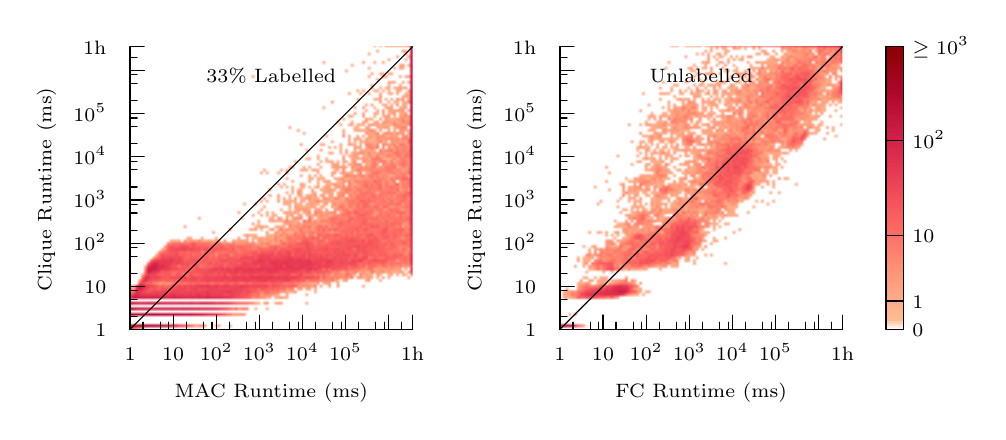
\begin{tikzpicture}[gnuplot]
%% generated with GNUPLOT 5.0p0 (Lua 5.2; terminal rev. 99, script rev. 100)
%% Tue 19 Apr 2016 16:47:16 AEST
\tikzset{every node/.append style={font={\scriptsize}}}
% \path (0.000,0.000) rectangle (10.922,7.366);
\gpcolor{color=gp lt color border}
\gpsetlinetype{gp lt border}
\gpsetdashtype{gp dt solid}
\gpsetlinewidth{1.00}
\draw[gp path] (1.320,5.785)--(1.320,2.197)--(4.908,2.197);
\node[gp node center,rotate=-270] at (0.246,3.991) {Clique Runtime (ms)};
\node[gp node center] at (3.114,1.427) {MAC Runtime (ms)};
\begin{scope}
\clip (1.320,5.785) rectangle (4.908,2.197);
\def\gprawrgbimagedata{%
  ffffffffffffffffffffffffffffffffffffffffffffffffffffffffffffffffffffffffffffffffffffffffffffffff%
  ffffffffffffffffffffffffffffffffffffffffffffffffffffffffffffffffffffffffffffffffffffffffffffffff%
  ffffffffffffffffffffffffffffffffffffffffffffffffffffffffffffffffffffffffffffffffffffffffffffffff%
  ffffffffffffffffffffffffffffffffffffffffffffffffffffffffffffffffffffffffffffffffffffffffffffffff%
  ffffffffffffffffffffffffffffffffffffffffffffffffffffffffffffffffffffffffffffffffffffffffffffffff%
  ffffffffffffffffffffffffffffffffffffffffffffac88ffffffffac88ffffffff9f7dff9f7dff9f7dffac88ff9f7d%
  ff9f7dffac88ff9576ff95768b0000ffffffffffffffffffffffffffffffffffffffffffffffffffffffffffffffffff%
  ffffffffffffffffffffffffffffffffffffffffffffffffffffffffffffffffffffffffffffffffffffffffffffffff%
  ffffffffffffffffffffffffffffffffffffffffffffffffffffffffffffffffffffffffffffffffffffffffffffffff%
  ffffffffffffffffffffffffffffffffffffffffffffffffffffffffffffffffffffffffffffffffffffffffffffffff%
  ffffffffffffffffffffffffffffffffffffffffffffffffffffffffffffffffffffffffffffffffffffffffffffffff%
  ffffffffffffffffffffffffffffffffffffffffffffffffffffffffffffffffffffffffffffffffffffffffffffffff%
  ffffffffffffffffffffffffffffffffffffffffffffffffffffffcf1d45ffffffffffffffffffffffffffffffffffff%
  ffffffffffffffffffffffffffffffffffffffffffffffffffffffffffffffffffffffffffffffffffffffffffffffff%
  ffffffffffffffffffffffffffffffffffffffffffffffffffffffffffffffffffffffffffffffffffffffffffffffff%
  ffffffffffffffffffffffffffffffffffffffffffffffffffffffffffffffffffffffffffffffffffffffffffffffff%
  ffffffffffffffffffffffffffffffffffffffffffffffffffffffffffffffffffffffffffffffffffffffffffffffff%
  ffffffffffffffffffffffffffffffffffffffffffffffffffffffffffffffffffffffffffffffffffffffffffffffff%
  ffffffffffffffac88ffffffffffffffffffffffffffffffffffffffffffffffffff9f7dffac88ffffffca1941ffffff%
  ffffffffffffffffffffffffffffffffffffffffffffffffffffffffffffffffffffffffffffffffffffffffffffffff%
  ffffffffffffffffffffffffffffffffffffffffffffffffffffffffffffffffffffffffffffffffffffffffffffffff%
  ffffffffffffffffffffffffffffffffffffffffffffffffffffffffffffffffffffffffffffffffffffffffffffffff%
  ffffffffffffffffffffffffffffffffffffffffffffffffffffffffffffffffffffffffffffffffffffffffffffffff%
  ffffffffffffffffffffffffffffffffffffffffffffffffffffffffffffffffffffffffffffffffffffffffffffffff%
  ffffffffffffffffffffffffffac88ffffffffffffffffffffffffffffffffffffffffffffffffffffffffffffffffff%
  ffffffffac88ffffffc7173effffffffffffffffffffffffffffffffffffffffffffffffffffffffffffffffffffffff%
  ffffffffffffffffffffffffffffffffffffffffffffffffffffffffffffffffffffffffffffffffffffffffffffffff%
  ffffffffffffffffffffffffffffffffffffffffffffffffffffffffffffffffffffffffffffffffffffffffffffffff%
  ffffffffffffffffffffffffffffffffffffffffffffffffffffffffffffffffffffffffffffffffffffffffffffffff%
  ffffffffffffffffffffffffffffffffffffffffffffffffffffffffffffffffffffffffffffffffffffffffffffffff%
  ffffffffffffffffffffffffffffffffffffffffffffffffffffffffffffffffffffffffffffffffffffffffffffffff%
  ffffffffffffffffffffac88ffffffffffffffffffffac88c7173effffffffffffffffffffffffffffffffffffffffff%
  ffffffffffffffffffffffffffffffffffffffffffffffffffffffffffffffffffffffffffffffffffffffffffffffff%
  ffffffffffffffffffffffffffffffffffffffffffffffffffffffffffffffffffffffffffffffffffffffffffffffff%
  ffffffffffffffffffffffffffffffffffffffffffffffffffffffffffffffffffffffffffffffffffffffffffffffff%
  ffffffffffffffffffffffffffffffffffffffffffffffffffffffffffffffffffffffffffffffffffffffffffffffff%
  ffffffffffffffffffffffffffffffffffffffffffffffffffffffffffffffffffffffffffffffffffffffffffffffff%
  ffffffffffffffffffffffffffffffffac88ffffffffffffffffffffffffffffffffac88ffffffc6163dffffffffffff%
  ffffffffffffffffffffffffffffffffffffffffffffffffffffffffffffffffffffffffffffffffffffffffffffffff%
  ffffffffffffffffffffffffffffffffffffffffffffffffffffffffffffffffffffffffffffffffffffffffffffffff%
  ffffffffffffffffffffffffffffffffffffffffffffffffffffffffffffffffffffffffffffffffffffffffffffffff%
  ffffffffffffffffffffffffffffffffffffffffffffffffffffffffffffffffffffffffffffffffffffffffffffffff%
  ffffffffffffffffffffac88ffffffffffffffffffffffffffffffffffffffffffffffffffffffffffffffffffffffff%
  ffffffffac88ffffffffffffffffffffac88ffffffffffffffac88ffffffffffffffffffffffffffffffffffffffffff%
  ffffffffffffc6163effffffffffffffffffffffffffffffffffffffffffffffffffffffffffffffffffffffffffffff%
  ffffffffffffffffffffffffffffffffffffffffffffffffffffffffffffffffffffffffffffffffffffffffffffffff%
  ffffffffffffffffffffffffffffffffffffffffffffffffffffffffffffffffffffffffffffffffffffffffffffffff%
  ffffffffffffffffffffffffffffffffffffffffffffffffffffffffffffffffffffffffffffffffffffffffffffffff%
  ffffffffffffffffffffffffffffffffffffffffffffffffffffffffffffffffffffffffffffffffffffffffffffffff%
  ffffffffffffffac88ffffffffffffffffffffffffffffffffffffffffffffffffffffffffffffffffffffffffffffff%
  ffffffffffffffffffffac88ff9576ffffffffac88c7173fffffffffffffffffffffffffffffffffffffffffffffffff%
  ffffffffffffffffffffffffffffffffffffffffffffffffffffffffffffffffffffffffffffffffffffffffffffffff%
  ffffffffffffffffffffffffffffffffffffffffffffffffffffffffffffffffffffffffffffffffffffffffffffffff%
  ffffffffffffffffffffffffffffffffffffffffffffffffffffffffffffffffffffffffffffffffffffffffffffffff%
  ffffffffffffffffffffffffffffffffffffffffffffffffffffffffffffffffffffffffffffffffffffffffffffffff%
  ffffffffffffffffffffffffffffffffffffffffffffffffffffffffffffffffffffffffffffffffac88ffffffffffff%
  ffffffffffffffffffffffffffffffffffffffac88ffffffff9f7dffac88ffffffffffffc1133affffffffffffffffff%
  ffffffffffffffffffffffffffffffffffffffffffffffffffffffffffffffffffffffffffffffffffffffffffffffff%
  ffffffffffffffffffffffffffffffffffffffffffffffffffffffffffffffffffffffffffffffffffffffffffffffff%
  ffffffffffffffffffffffffffffffffffffffffffffffffffffffffffffffffffffffffffffffffffffffffffffffff%
  ffffffffffffffffffffffffffffffffffffffffffffffffffffffffffffffffffffffffffffffffffffffffffffffff%
  ffffffffffffffffffffffffffffffffffffffffffffffffffffffffffffffac88ffffffffffffffffffffffffffffff%
  ffffffffffffffffffffffffffffffffffffffffffffffffffffffffffffffffffffffffffffffffffffffffffffffff%
  ffffffc8183fffffffffffffffffffffffffffffffffffffffffffffffffffffffffffffffffffffffffffffffffffff%
  ffffffffffffffffffffffffffffffffffffffffffffffffffffffffffffffffffffffffffffffffffffffffffffffff%
  ffffffffffffffffffffffffffffffffffffffffffffffffffffffffffffffffffffffffffffffffffffffffffffffff%
  ffffffffffffffffffffffffffffffffffffffffffffffffffffffffffffffffffffffffffffffffffffffffffffffff%
  ffffffffffffffffffffffffffffffffffffffffffffffffffffffffffffffffffffffffffffffffffffffffffffffff%
  ffffffffffffffffffffffffffffffffffffffffffffffffffac88ffffffffffffffac88ffac88ffffffffac88ffac88%
  ffffffffffffffffffffffffffffffffffffc8183fffffffffffffffffffffffffffffffffffffffffffffffffffffff%
  ffffffffffffffffffffffffffffffffffffffffffffffffffffffffffffffffffffffffffffffffffffffffffffffff%
  ffffffffffffffffffffffffffffffffffffffffffffffffffffffffffffffffffffffffffffffffffffffffffffffff%
  ffffffffffffffffffffac88ffffffffffffffffffffffffffffffffffffffffffffffffffffffffffffffffffffffff%
  ffffffffffffffffffffffffffffffffffffffffffffffffffffffffffffffffffffffffffffffffffffffffffffffff%
  ffffffffffffffffffffffffffffffffffffffffffffffffffffffffffffffffffffffffffac88ffffffffffffffffff%
  ffffffffac88ffac88ffffffffffffffffffffffffffac88ffffffffac88ff9f7dc6163effffffffffffffffffffffff%
  ffffffffffffffffffffffffffffffffffffffffffffffffffffffffffffffffffffffffffffffffffffffffffffffff%
  ffffffffffffffffffffffffffffffffffffffffffffffffffffffffffffffffffffffffffffffffffffffffffffffff%
  ffffffffffffffffffffffffffffffffffffffffffffffffffffffffffffffffffffffffffffffffffffffffffffffff%
  ffffffffffffffffffffffffffffffffffffffffffffffffffffffffffffffffffffffffffffffffffffffffffffffff%
  ffffffffffffffffffffffffffffffffffffffffffffffffffffffffffffffffffffffffffffffffffffffffffffffff%
  ffffffffffffffffffffffffffac88ffffffffffffffffffffffffffffffffffffffffffffffffffffffffffffffffff%
  c8183fffffffffffffffffffffffffffffffffffffffffffffffffffffffffffffffffffffffffffffffffffffffffff%
  ffffffffffffffffffffffffffffffffffffffffffffffffffffffffffffffffffffffffffffffffffffffffffffffff%
  ffffffffffffffffffffffffffffffffffffffffffffffffffffffffffffffffffffffffffffffffffffffffffffffff%
  ffffffffffffffffffffffffffffffffffffffffffffffffffffffffffffffffffffffffffffffffffffffffffffffff%
  ffffffffffffffffffffffffffffffffffffffffffffffffffffffffffffffffffffffffffffffffffffffffffffffff%
  ffffffffffffffffffffffffffffffffffffffffffffffffffffffffffffffffffffffffffffffffac88ffac88ffac88%
  ffffffffffffffac88ffffffffac88c4153cffffffffffffffffffffffffffffffffffffffffffffffffffffffffffff%
  ffffffffffffffffffffffffffffffffffffffffffffffffffffffffffffffffffffffffffffffffffffffffffffffff%
  ffffffffffffffffffffffffffffffffffffffffffffffffffffffffffffffffffffffffffffffffffffffffffffffff%
  ffffffffffffffffffffffffffffffffffffffffffffffffffffffffffffffffffffffffffffffffffffffffffffffff%
  ffffffffffffffffffffffffffffffffffffffffffffffffffffffffffffffffffffffffffffffffffffffffffffffff%
  ffffffffffffffffffffffffffffffffffffffffffffffffffffffffffffffffffffffffffac88ffffffffffffffffff%
  ffffffffffffffac88ffffffffffffffffffffac88ffffffffffffffffffc4143cffffffffffffffffffffffffffffff%
  ffffffffffffffffffffffffffffffffffffffffffffffffffffffffffffffffffffffffffffffffffffffffffffffff%
  ffffffffffffffffffffffffffffffffffffffffffffffffffffffffffffffffffffffffffffffffffffffffffffffff%
  ffffffffffffffffffffffffffffffffffffffffffffffffffffffffffffffffffffffffffffffffffffffffffffffff%
  ffffffffffffffffffffffffffffffffffffffffffffffffffffffffffffffffffffffffffffffffffffffffffffffff%
  ffffffffffffffffffffffffffffffffffffffffffffffffffffffffffffffffffffffffffffffffffffffffffffffff%
  ffffffffac88ffffffffffffffac88ffffffffac88ffac88ffffffffac88ffac88ff9f7dffac88ff9f7dffffffc3143b%
  ffffffffffffffffffffffffffffffffffffffffffffffffffffffffffffffffffffffffffffffffffffffffffffffff%
  ffffffffffffffffffffffffffffffffffffffffffffffffffffffffffffffffffffffffffffffffffffffffffffffff%
  ffffffffffffffffffffffffffffffffffffffffffffffffffffffffffffffffffffffffffffffffffffffffffffffff%
  ffffffffffffffffffffffffffffffffffffffffffffffffffffffffffffffffffffffffffffffffffffffffffffffff%
  ffffffffffffffffffffffffffffffffffffffffffffffffffffffffffffffffffffffffffffffffffffffffffffffff%
  ffffffffac88ffffffffac88ffffffffffffffffffffac88ffac88ffffffffac88ffffffffac88ffffffffffffff9f7d%
  ffac88ffffffffffffff9f7dc1133affffffffffffffffffffffffffffffffffffffffffffffffffffffffffffffffff%
  ffffffffffffffffffffffffffffffffffffffffffffffffffffffffffffffffffffffffffffffffffffffffffffffff%
  ffffffffffffffffffffffffffffffffffffffffffffffffffffffffffffffffffffffffffffffffffffffffffffffff%
  ffffffffffffffffffffffffffffffffffffffffffffffffffffffffffffffffffffffffffffffffffffffffffffffff%
  ffffffffffffffffffffffffffffffffffffffffffffffffffffffffffffffffffffffffffffffffffffffffffffffff%
  ffffffffffffffffffffac88ffffffffffffffffffffac88ffffffffffffffac88ffffffffffffffffffffac88ffffff%
  ffffffffac88ffac88ffffffffac88ffffffffffffffac88ffac88c4153cffffffffffffffffffffffffffffffffffff%
  ffffffffffffffffffffffffffffffffffffffffffffffffffffffffffffffffffffffffffffffffffffffffffffffff%
  ffffffffffffffffffffffffffffffffffffffffffffffffffffffffffffffffffffffffffffffffffffffffffffffff%
  ffffffffffffffffffffffffffffffffffffffffffffffffffffffffffffffffffffffffffffffffffffffffffffffff%
  ffffffffffffffffffffffffffffffffffffffffffffffffffffffffffffffffffffffffffffffffffffffffffffffff%
  ffffffffffffffffffffffffffffffffffffffffffffffffffffffffffffffffffffffffffffffffffffffffffffffff%
  ffffffffffffffffffff9576ffffffffffffffffffffffffffffffffffffffffffffac88ff9f7dffac88c2133affffff%
  ffffffffffffffffffffffffffffffffffffffffffffffffffffffffffffffffffffffffffffffffffffffffffffffff%
  ffffffffffffffffffffffffffffffffffffffffffffffffffffffffffffffffffffffffffffffffffffffffffffffff%
  ffffffffffffffffffffffffffffffffffffffffffffffffffffffffffffffffffffffffffffffffffffffffffffffff%
  ffffffffffffffffffffffffffffffffffffffffffffffffffffffffffffffffffffffffffffffffffffffffffffffff%
  ffffffffffffffffffffffffffffffffffffffffffffffffffffffffffffffffffffffffffffffffffffffffffffffff%
  ffac88ffffffffffffffffffffffffffffffffac88ffac88ffac88ffffffffac88ffffffffac88ffffffff9576ffac88%
  ff9576ffffffff9f7dc6163dffffffffffffffffffffffffffffffffffffffffffffffffffffffffffffffffffffffff%
  ffffffffffffffffffffffffffffffffffffffffffffffffffffffffffffffffffffffffffffffffffffffffffffffff%
  ffffffffffffffffffffffffffffffffffffffffffffffffffffffffffffffffffffffffffffffffffffffffffffffff%
  ffffffffffffffffffffffffffffffffffffffffffffffffffffffffffffffffffffffffffffffffffffffffffffffff%
  ffffffffffffffffffffffffffffffffffffffffffffffffffffffffffffffffffffffffff9f7dffffffffffffffffff%
  ffffffffffffffffffffffffffffffffffffffffffffffffffffffffffffffffffffffffffffffff9f7dffffffffffff%
  ffac88ffffffffac88ffac88ffffffffac88ffac88ff846ec01239ffffffffffffffffffffffffffffffffffffffffff%
  ffffffffffffffffffffffffffffffffffffffffffffffffffffffffffffffffffffffffffffffffffffffffffffffff%
  ffffffffffffffffffffffffffffffffffffffffffffffffffffffffffffffffffffffffffffffffffffffffffffffff%
  ffffffffffffffffffffffffffffffffffffffffffffffffffffffffffffffffffffffffffffffffffffffffffffffff%
  ffffffffffffffffffffffffffffffffffffffffffffffffffffffffffffffffffffffffffffffffffffffffffffffff%
  ffffffffffffffffffffffffffffffffffffffffffffffffffffffffffffffffffffffffffffffffac88ffffffff9f7d%
  ffffffffffffffffffffac88ffac88ffffffffac88ffffffff9576ffffffffac88ffac88ffffffc4153cffffffffffff%
  ffffffffffffffffffffffffffffffffffffffffffffffffffffffffffffffffffffffffffffffffffffffffffffffff%
  ffffffffffffffffffffffffffffffffffffffffffffffffffffffffffffffffffffffffffffffffffffffffffffffff%
  ffffffffffffffffffffffffffffffffffffffffffffffffffffffffffffffffffffffffffffffffffffffffffffffff%
  ffffffffffffffffffffffffffffffffffffffffffffffffffffffffffffffffffffffffffffffffffffffffffffffff%
  ffffffffffffffffffffac88ffffffffffffffffffffffffffffffffffffffffffffffffffffffffffffffac88ffffff%
  ffffffff9f7dffffffffffffffffffffac88ffffffffffffffffffffac88ff9f7dff9f7dffffffffffffffac88ff9f7d%
  ff9f7dffffffbd0f36ffffffffffffffffffffffffffffffffffffffffffffffffffffffffffffffffffffffffffffff%
  ffffffffffffffffffffffffffffffffffffffffffffffffffffffffffffffffffffffffffffffffffffffffffffffff%
  ffffffffffffffffffffffffffffffffffffffffffffffffffffffffffffffffffffffffffffffffffffffffffffffff%
  ffffffffffffffffffffffffffffffffffffffffffffffffffffffffffffffffffffffffffffffffffffffffffffffff%
  ffffffffffffffffffffffffffffffffffffffffffffffffffffffffffffffffffffffffffffffffffffffffffffffff%
  ffffffffffffffffffffffffffffffffffffffffffffac88ffffffffffffffffffffac88ffffffff9576ffffffffac88%
  ff9f7dffac88ff9576ff9f7dff9576ffffffffac88c2133affffffffffffffffffffffffffffffffffffffffffffffff%
  ffffffffffffffffffffffffffffffffffffffffffffffffffffffffffffffffffffffffffffffffffffffffffffffff%
  ffffffffffffffffffffffffffffffffffffffffffffffffffffffffffffffffffffffffffffffffffffffffffffffff%
  ffffffffffffffffffffffffffffffffffffffffffffffffffffffffffffffffffffffffffffffffffffffffffffffff%
  ffffffffffffffffffffffffffffffffffffffffffffffffffffffffffffffffffffffffffffffffffffffffffffffff%
  ffffffffffffffffffffffffffffffffffffffffffffffffff9f7dffffffffffffffac88ffffffffffffffffffffac88%
  ffac88ffffffff9f7dffffffffac88ffac88ff9576ffffffffac88ff9f7dff9576ffffffc1133affffffffffffffffff%
  ffffffffffffffffffffffffffffffffffffffffffffffffffffffffffffffffffffffffffffffffffffffffffffffff%
  ffffffffffffffffffffffffffffffffffffffffffffffffffffffffffffffffffffffffffffffffffffffffffffffff%
  ffffffffffffffffffffffffffffffffffffffffffffffffffffffffffffffffffffffffffffffffffffffffffffffff%
  ffffffffffffffffffffffffffffffffffffffffffffffffffffffffffffffffffffffffffffffffffffffffffffffff%
  ffffffffffffffffffffffffffffffffffffffffffffffffffffffffffffffffffffac88ffac88ffffffffffffffffff%
  ff9f7dffffffffffffffffffffac88ffffffffffffffac88ff9f7dff9576ffffffffac88ffffffff9f7dff9f7dff8c72%
  ff9f7dc01238ffffffffffffffffffffffffffffffffffffffffffffffffffffffffffffffffffffffffffffffffffff%
  ffffffffffffffffffffffffffffffffffffffffffffffffffffffffffffffffffffffffffffffffffffffffffffffff%
  ffffffffffffffffffffffffffffffffffffffffffffffffffffffffffffffffffffffffffffffffffffffffffffffff%
  ffffffffffffffffffffffffffffffffffffffffffffffffffffffffffffffffffffffffffffffffffffffffffffffff%
  ffffffffffffffffffffffffffffffffffffffffffffffffffffffffffffffffffffffffffffffffffffffac88ffffff%
  ffffffffffffffffffffffffffffffffffffff9f7dffac88ffac88ffffffffffffff9f7dffffffff9576ffac88ffac88%
  ffac88ff9f7dff9576ff846effac88ffac88c1133affffffffffffffffffffffffffffffffffffffffffffffffffffff%
  ffffffffffffffffffffffffffffffffffffffffffffffffffffffffffffffffffffffffffffffffffffffffffffffff%
  ffffffffffffffffffffffffffffffffffffffffffffffffffffffffffffffffffffffffffffffffffffffffffffffff%
  ffffffffffffffffffffffffffffffffffffffffffffffffffffffffffffffffffffffffffffffffffffffffffffffff%
  ffffffffffffffffffffffffffffffffffffffffffffffffffffffffffffffffffffffffffffffffffffffffffffffff%
  ffffffffac88ffffffffffffffffffffffffffac88ffffffffffffffffffffac88ff9f7dffffffffffffffac88ff9f7d%
  ffffffff9f7dff9576ff9f7dffac88ff9576ffac88ff9f7dff846eff8c72ff8c72c3143bffffffffffffffffffffffff%
  ffffffffffffffffffffffffffffffffffffffffffffffffffffffffffffffffffffffffffffffffffffffffffffffff%
  ffffffffffffffffffffffffffffffffffffffffffffffffffffffffffffffffffffffffffffffffffffffffffffffff%
  ffffffffffffffffffffffffffffffffffffffffffffffffffffffffffffffffffffffffffffffffffffffffffffffff%
  ffffffffffffffffffffffffffffffffffffffffffffffffffffffffffffffffffffffffffffffffffffffffffffffff%
  ffffffffffffffffffffffffffffffffffffffffffffac88ffffffffffffffac88ff9f7dffffffffac88ffac88ffac88%
  ffffffff9f7dff9f7dff9f7dff9f7dffac88ff9f7dffac88ffac88ffac88ff846eff9576ff9f7dff9f7dff9f7dff9576%
  c11239ffffffffffffffffffffffffffffffffffffffffffffffffffffffffffffffffffffffffffffffffffffffffff%
  ffffffffffffffffffffffffffffffffffffffffffffffffffffffffffffffffffffffffffffffffffffffffffffffff%
  ffffffffffffffffffffffffffffffffffffffffffffffffffffffffffffffffffffffffffffffffffffffffffffffff%
  ffffffffffffffffffffffffffffffffffffffffffffffffffffffffffffffac88ffffffffffffffffffffffffffffff%
  ffffffffffffffffffffffffffffffffffffffffffffffffffffffffffffffffffffffffffffffffffffffffffffffff%
  ffffffffac88ffac88ffffffffffffff9f7dffac88ffffffffffffffac88ffac88ffac88ff9576ffac88ffffffffac88%
  ff9576ff9576ff846eff846effffffbd1036ffffffffffffffffffffffffffffffffffffffffffffffffffffffffffff%
  ffffffffffffffffffffffffffffffffffffffffffffffffffffffffffffffffffffffffffffffffffffffffffffffff%
  ffffffffffffffffffffffffffffffffffffffffffffffffffffffffffffffffffffffffffffffffffffffffffffffff%
  ffffffffffffffffffffffffffffffffffffffffffffffffffffffffffffffffffffffffffffffffffffffffffffffff%
  ffffffffffffffac88ffffffffffffffffffffffffffffffffffffffffffffffffffffffffffffffffffffffffffffff%
  ffffffffffffffac88ffffffffffffffffffffac88ffac88ffac88ffac88ffac88ff9576ff846eff9f7dffffffff9f7d%
  ffffffffffffff9f7dffffffff9f7dffffffff9576ff9576ffac88ffac88c01239ffffffffffffffffffffffffffffff%
  ffffffffffffffffffffffffffffffffffffffffffffffffffffffffffffffffffffffffffffffffffffffffffffffff%
  ffffffffffffffffffffffffffffffffffffffffffffffffffffffffffffffffffffffffffffffffffffffffffffffff%
  ffffffffffffffffffffffffffffffffffffffffffffffffffffffffffffffffffffffffffffffffffffffffffffffff%
  ffffffffffffffffffffffffffffffffffffffffffffffffffffffffac88ffffffffffffffffffffffffffffffffffff%
  ffffffffffffffffffffffffffffffffffffffffffffac88ffffffffffffffffffffffffffffffffffffffffffff9576%
  ffac88ffac88ff9f7dff846effffffffac88ff846eff9576ff9576ffac88ff8c72ff9f7dff8c72ffffffff9f7dbf1138%
  ffffffffffffffffffffffffffffffffffffffffffffffffffffffffffffffffffffffffffffffffffffffffffffffff%
  ffffffffffffffffffffffffffffffffffffffffffffffffffffffffffffffffffffffffffffffffffffffffffffffff%
  ffffffffffffffffffffffffffffffffffffffffffffffffffffffffffffffffffffffffffffffffffffffffffffffff%
  ffffffffffffffffffffffffffffffffffffffffffffffffffffffffffffffffffffffffffffffffffffffffffffffff%
  ffffffffffffffffffffffffffffffffffffffac88ffffffffffffffffffffffffffffffff9576ffffffffac88ffffff%
  ffffffffac88ffffffffac88ffffffff9576ff9f7dffac88ff8c72ff9576ff8c72ffac88ffac88ff9f7dff9f7dffac88%
  ffffffff8c72ff846effac88c11239ffffffffffffffffffffffffffffffffffffffffffffffffffffffffffffffffff%
  ffffffffffffffffffffffffffffffffffffffffffffffffffffffffffffffffffffffffffffffffffffffffffffffff%
  ffffffffffffffffffffffffffffffffffffffffffffffffffffffffffffffffffffffffffffffffffffffffffffffff%
  ffffffffffffffffffffffffffffffffffffffffffffffffffffffffffffffffffffffffffffffffffffffffffffffff%
  ffffffffffffffffffffffffffffffffffffffffffffffffffffffffffffffffffffffffffffffffffffffffffffffff%
  ffffffffffffffffffffac88ffffffff9f7dff9f7dffac88ffffffff9f7dff9f7dffac88ffac88ff8c72ff9f7dff9f7d%
  ff8c72ff9576ff8c72ff9f7dff8c72ff9f7dff846eff8c72ff7e6cc11239ffffffffffffffffffffffffffffffffffff%
  ffffffffffffffffffffffffffffffffffffffffffffffffffffffffffffffffffffffffffffffffffffffffffffffff%
  ffffffffffffffffffffffffffffffffffffffffffffffffffffffffffffffffffffffffffffffffffffffffffffffff%
  ffffffffffffffffffffffffffffffffffffffffffffffffffffffffffffffffffffffffffffffffffffffffffffffff%
  ffffffffffffffffffffffffffffffffffffffffffffffffffffffffffffffffffffffffffffffffffffffffffffffff%
  ffffffffffffffac88ffffffffffffffffffffffffffffffffac88ffffffffac88ffffffffac88ffac88ff9f7dffac88%
  ffac88ffac88ff9f7dff7e6cffac88ff9f7dffffffff9576ff9f7dff9576ff9f7dff9576ffac88fb605fc2133bffffff%
  ffffffffffffffffffffffffffffffffffffffffffffffffffffffffffffffffffffffffffffffffffffffffffffffff%
  ffffffffffffffffffffffffffffffffffffffffffffffffffffffffffffffffffffffffffffffffffffffffffffffff%
  ffffffffffffffffffffffffffffffffffffffffffffffffffffffffffffffffffffffffffffffffffffffffffffffff%
  ffffffffffffffffffffffffffffffffffffffffffffffffffffffffffffffffffffffffffac88ffffffffffffffffff%
  ffffffffffffffffffffac88ffac88ffffffffffffffffffffffffffffffffac88ffffffffffffff9f7dffac88ffac88%
  ffffffffac88ffffffff846eff846eff9576ffac88ff846effffffff8c72ff9576ff9f7dff9576ff846effac88ff7869%
  ff7e6cff9576ff8c72c4153cffffffffffffffffffffffffffffffffffffffffffffffffffffffffffffffffffffffff%
  ffffffffffffffffffffffffffffffffffffffffffffffffffffffffffffffffffffffffffffffffffffffffffffffff%
  ffffffffffffffffffffffffffffffffffffffffffffffffffffffffffffffffffffffffffffffffffffffffffffffff%
  ffffffffffffffffffffffffffffffffffffffffffffffffffffffffffffffffffffffffffffffffffffffffffffffff%
  ffffffffffffffffffffffffffffffffffffffffffffffffffffffffffffffffffffac88ffffffffac88ffffffffac88%
  ffffffffffffffffffffffffff9f7dff9f7dffac88ffffffffac88ff846eff846eff9576ff7869ffffffff8c72ffffff%
  ff8c72ffac88ff8c72ff7e6cff9576ff8c72ff846eff9576c01239ffffffffffffffffffffffffffffffffffffffffff%
  ffffffffffffffffffffffffffffffffffffffffffffffffffffffffffffffffffffffffffffffffffffffffffffffff%
  ffffffffffffffffffffffffffffffffffffffffffffffffffffffffffffffffffffffffffffffffffffffffffffffff%
  ffffffffffffffffffffffffffffffffffffffffffffffffffffffffffffffffffffffffffffffffffffffffffffffff%
  ffffffffffffffffffffffffffffffffffffffffffffffffffac88ffffffffffffffffffffffffff9f7dffffffffffff%
  ffffffffffffffffffffffffffac88ffffffffac88ffffffffffffff9f7dffffffffac88ffac88ff9f7dffac88ff9576%
  ffac88ffffffff846eff9f7dff8c72ff846eff7e6cff9f7dff7869ff9576ff7e6cff8c72ff7e6cc1133affffffffffff%
  ffffffffffffffffffffffffffffffffffffffffffffffffffffffffffffffffffffffffffffffffffffffffffffffff%
  ffffffffffffffffffffffffffffffffffffffffffffffffffffffffffffffffffffffffffffffffffffffffffffffff%
  ffffffffffffffffffffffffffffffffffffffffffffffffffffffffffffffffffffffffffffffffffffffffffffffff%
  ffffffffffffffffffffffffffffffffffffffffffffffffffffffffffffffffffffffffffffffffffffffffffffffff%
  ffffffffffffffffffffffffffffffffac88ffac88ffffffffffffffac88ffffffff9f7dffffffffac88ff9f7dff9576%
  ff8c72ff9576ffac88ff7e6cffac88ff9f7dffac88ff846eff8c72ff9f7dff9576ff9576ff7367ff6f65ff846eff8c72%
  ff7e6cff7e6cc3143bffffffffffffffffffffffffffffffffffffffffffffffffffffffffffffffffffffffffffffff%
  ffffffffffffffffffffffffffffffffffffffffffffffffffffffffffffffffffffffffffffffffffffffffffffffff%
  ffffffffffffffffffffffffffffffffffffffffffffffffffffffffffffffffffffffffffffffffffffffffffffffff%
  ffffffffffffffffffffffffffffffffffffffffffffffffffffffffffffffffffffffffffffffffffffffffffffffff%
  ffffffffffffffffffffffffffffffffffffffac88ffffffffffffffffffffffffffffffffffffffffffffffffffac88%
  ffffffffac88ffac88ff9576ffac88ffffffffac88ffac88ff9576ff9f7dffac88ff7869ffac88ff9f7dff8c72ff7869%
  ff8c72ff9f7dff7367ff7e6cff9576ff6f65ff7e6cc6163dffffffffffffffffffffffffffffffffffffffffffffffff%
  ffffffffffffffffffffffffffffffffffffffffffffffffffffffffffffffffffffffffffffffffffffffffffffffff%
  ffffffffffffffffffffffffffffffffffffffffffffffffffffffffffffffffffffffffffffffffffffffffffffffff%
  ffffffffffffffffffffffffffffffffffffffffffffffffffffffffffffffffffffffffffffffffffffffffffffffff%
  ffffffffffffffffffffffffffffffffffffffffffffac88ffac88ffffffffffffffac88ffffffffffffffac88ffffff%
  ffffffffffffffffffffffffff9576ffffffffffffff9f7dffac88ff9f7dffac88ff9576ff9f7dffac88ff846eff7e6c%
  ff7869ff846effac88ffac88ffac88ff9f7dff7e6cffac88ff846eff7869ff8c72ff8c72c4153cffffffffffffffffff%
  ffffffffffffffffffffffffffffffffffffffffffffffffffffffffffffffffffffffffffffffffffffffffffffffff%
  ffffffffffffffffffffffffffffffffffffffffffffffffffffffffffffffffffffffffffffffffffffffffffffffff%
  ffffffffffffffffffffffffffffffffffffffffffffffffffffffffffffffffffffffffffffffffffffffffffffffff%
  ffffffffffffffffffffffffffffffffffffffffffffffffffac88ffffffffffffffffffffffffffffffffffffffffff%
  ffffffffac88ffffffffac88ffac88ffac88ffffffffac88ffffffffac88ffac88ffffffffac88ff8c72ffffffffffff%
  ff8c72ff9f7dff9f7dff9576ff7869ff9f7dff7e6cff7869ff8c72ffac88ff7869ffac88ff8c72ff8c72ff7869ff7e6c%
  ff9576c4153cffffffffffffffffffffffffffffffffffffffffffffffffffffffffffffffffffffffffffffffffffff%
  ffffffffffffffffffffffffffffffffffffffffffffffffffffffffffffffffffffffffffffffffffffffffffffffff%
  ffffffffffffffffffffffffffffffffffffffffffffffffffffffffffffffffffffffffffffffffffffffffffffffff%
  ffffffffffffffffffffffffffffffffffffffffffffffffffffffffffffffffffffffffffffffffffffffffffffffff%
  ffffffffffffffffffffffffffffffffac88ffffffffffffffffffffffffffac88ff9f7dff9f7dffffffffac88ffffff%
  ff9f7dffac88ff8c72ff8c72ff9576ffffffff9f7dffac88ff846eff7869ff9576ffffffff846eff9576ff8c72ff7869%
  ff846eff9576ff7e6cff6b63ff7e6cff8c72cb1a41ffffffffffffffffffffffffffffffffffffffffffffffffffffff%
  ffffffffffffffffffffffffffffffffffffffffffffffffffffffffffffffffffffffffffffffffffffffffffffffff%
  ffffffffffffffffffffffffffffffffffffffffffffffffffffffffffffffffffffffffffffffffffffffffffffffff%
  ffffffffffffffffffffffffffffffffffffffffffffffffffffffffffffffffffffffffffffffffffffffffffffffff%
  ffac88ffac88ffffffffffffffffffffac88ffffffffac88ffffffffffffffffffffac88ffffffffffffffffffffac88%
  ff9f7dff9f7dff9f7dff9576ffac88ffffffff8c72ff9f7dffac88ff8c72ff9f7dff8c72ff9576ff7e6cff7869ffac88%
  ff8c72ff9576ff7869ff846eff7e6cff6b63ffac88ff9576ff846eff9576ff8c72c8183fffffffffffffffffffffffff%
  ffffffffffffffffffffffffffffffffffffffffffffffffffffffffffffffffffffffffffffffffffffffffffffffff%
  ffffffffffffffffffffffffffffffffffffffffffffffffffffffffffffffffffffffffffffffffffffffffffffffff%
  ffffffffffffffffffffffffffffffffffffffffffffffffffffffffffffffffffffffffffac88ffffffffffffffffff%
  ffffffffffffffac88ffffffffac88ffffffffffffffffffffffffffac88ffac88ffac88ffffffffac88ff9f7dffac88%
  ffffffffffffffffffffffffffffffffac88ffac88ffffffff846effffffffffffffac88ff9f7dff7869ff8c72ff8c72%
  ff9576ff8c72ff846eff9576ff7e6cff846eff846eff7e6cff7367ff7e6cff9576ff7e6cff8c72ff9f7dff9f7dff7e6c%
  c8183fffffffffffffffffffffffffffffffffffffffffffffffffffffffffffffffffffffffffffffffffffffffffff%
  ffffffffffffffffffffffffffffffffffffffffffffffffffffffffffffffffffffffffffffffffffffffffffffffff%
  ffffffffffffffffffffffffffffffffffffffffffffffffffffffffffffffffffffffffffffffffffffffffffffffff%
  ffac88ffffffffac88ffffffffffffffffffffac88ffffffffffffff9f7dffffffffffffffffffffffffffffffffffff%
  ffffffffffffffffffffffffffac88ffffffffffffffffffffffffff9f7dff9f7dffffffffac88ff9576ffac88ffac88%
  ff9f7dffffffffac88ff846effffffffac88ff9f7dff846eff6f65ff7367ff846eff9576ff8c72ff846eff846eff7e6c%
  ff9576ff846eff8c72ff8c72ff6b63c8183fffffffffffffffffffffffffffffffffffffffffffffffffffffffffffff%
  ffffffffffffffffffffffffffffffffffffffffffffffffffffffffffffffffffffffffffffffffffffffffffffffff%
  ffffffffffffffffffffffffffffffffffffffffffffffffffffffffffffffffffffffffffffffffffffffffffffffff%
  ffffffffffffffffffffffffffffffffffffffffffffffffffffffffffffffffffffffffffffffffffffffffffffffff%
  ffffffffffffffffffffac88ffffffffffffffac88ffffffffac88ffffffffac88ffffffffffffffffffffac88ffffff%
  ffffffffffffffac88ff7e6cff846eff9576ff846eff9f7dff846eff7e6cff9f7dff7e6cff7869ff8c72ff7e6cff9f7d%
  ff846eff8c72ff9f7dffac88ff9576ff846eff8c72ff7367ff846effac88c7173effffffffffffffffffffffffffffff%
  ffffffffffffffffffffffffffffffffffffffffffffffffffffffffffffffffffffffffffffffffffffffffffffffff%
  ffffffffffffffffffffffffffffffffffffffffffffffffffffffffffffffffffffffffffffffffffffffffffffffff%
  ffffffffffffffffffffffffffffffffffffffffffffffffffffffffffffffffffffffffffffffffffffffffffffffff%
  ffffffffffffffffffffac88ffffffffffffffffffffffffffffffffffffffffffffac88ffac88ffffffffac88ffac88%
  ffac88ffffffffffffffffffffac88ffac88ff9576ff9576ffac88ffac88ff9576ff9576ffac88ff9f7dff9576ff9576%
  ff9576ff7e6cff9576ff7e6cff7e6cff846eff8c72ff9576ff7869ff8c72ff7869ff7e6cfd6561fe6862ff7e6cc6163e%
  ffffffffffffffffffffffffffffffffffffffffffffffffffffffffffffffffffffffffffffffffffffffffffffffff%
  ffffffffffffffffffffffffffffffffffffffffffffffffffffffffffffffffffffffffffffffffffffffffffffffff%
  ffffffffffffffffffffffffffffffffffffffffffffffffffffffffffffffffffffffffffffffffffffffffffffffff%
  ffffffffffffffffffffffffffffffffffffffffffffffffffffffffffffffac88ffffffffffffffffffffffffffffff%
  ff9f7dffffffffffffffac88ffffffffac88ff9f7dffac88ffffffffffffffac88ffac88ff8c72ffac88ff846effac88%
  ff846eff7e6cff8c72ff7e6cff7e6cff846eff8c72fd6561ff7869ff7869ff9576ff7e6cff9576ff8c72ff7e6cffffff%
  ff9576ff7869ff8c72ff7367c8183fffffffffffffffffffffffffffffffffffffffffffffffffffffffffffffffffff%
  ffffffffffffffffffffffffffffffffffffffffffffffffffffffffffffffffffffffffffffffffffffffffffffffff%
  ffffffffffffffffffffffffffffffffffffffffffffffffffffffffffffffffffffffffffffffffffffffffffffffff%
  ffffffffffffffffffffffffffffffffffffffffffffffffffffffffffffffac88ffffffffac88ffffffffffffffffff%
  ffffffffffffff9f7dffac88ffffffffffffffffffffffffffac88ffffffffffffffac88ffac88ff9f7dff8c72ffac88%
  ffac88ff9f7dffffffff7e6cff9f7dffac88ff9576ff846eff7e6cfe6862ff846eff7869ff8c72ff6f65ff7367ff9576%
  ff7869ff846eff9f7dff7e6cfc6260ff9f7dff7869ff8c72ff7869cc1a42ffffffffffffffffffffffffffffffffffff%
  ffffffffffffffffffffffffffffffffffffffffffffffffffffffffffffffffffffffffffffffffffffffffffffffff%
  ffffffffffffffffffffffffffffffffffffffffffffffffffffffffffffffffffffffffffffffffffffffffffffffff%
  ffffffffffffffffffffffffffffffffffffffffffffffffffffffffffffffffffffffffffffffffffffffffffffffff%
  ffac88ffffffffac88ffffffffac88ffffffffffffffac88ffac88ffffffffac88ffffffffac88ff9f7dffffffffac88%
  ff9f7dff9f7dffffffffac88ff8c72ff9f7dff846effac88ff846eff9f7dff846eff9576ff8c72ff7e6cff6f65ff7869%
  ff7367ff846eff7869fe6862ff9576ff7869ff7e6cff6b63ff7e6cff7e6cff9576ff846eff7869ff846ec8183fffffff%
  ffffffffffffffffffffffffffffffffffffffffffffffffffffffffffffffffffffffffffffffffffffffffffffffff%
  ffffffffffffffffffffffffffffffffffffffffffffffffffffffffffffffffffffffffffffffffffffffffffffffff%
  ffffffffffffffffffffffffffffffffffffffffffffffffffffffffffffffffffffffffffffffffffffffffffffffff%
  ffffffffac88ffffffffffffffffffffffffffffffffffffffffffffac88ffffffffac88ffac88ffffffffffffffffff%
  ff9f7dffffffffffffffac88ffac88ff9f7dff9f7dff9576ffac88ffffffffac88ff8c72ff7869ff7869ff8c72ff9576%
  ff7367ff7869ff8c72ff8c72ff7367ff846eff7869ff846eff6f65ff846eff846eff7e6cff7869ff8c72fd6561ff9f7d%
  ff9576ff846eff9f7dcb1a41ffffffffffffffffffffffffffffffffffffffffffffffffffffffffffffffffffffffff%
  ffffffffffffffffffffffffffffffffffffffffffffffffffffffffffffffffffffffffffffffffffffffffffffffff%
  ffffffffffffffffffffffffffffffffffffffffffffffffffffffffffffffffffffffffffffffffffffffffffffffff%
  ffffffffffffffffffffffffffffffffffffffffffffffffffffffffffffffffffffffffffac88ffffffffac88ffffff%
  ff8c72ffac88ffffffffffffffffffffac88ffac88ffffffffffffffac88ffac88ff9f7dffac88ffffffffac88ff8c72%
  ff9576ff8c72ff9576ff9576ff7e6cff9f7dff6f65ff7869ff6b63ff7869ff7869ff846effac88ff846eff7367ff7e6c%
  ff6b63ff7869ff6f65ff8c72ff846eff846eff6b63fe6862ca1940ffffffffffffffffffffffffffffffffffffffffff%
  ffffffffffffffffffffffffffffffffffffffffffffffffffffffffffffffffffffffffffffffffffffffffffffffff%
  ffffffffffffffffffffffffffffffffffffffffffffffffffffffffffffffffffffffffffffffffffffffffffffffff%
  ffffffffffffffffffffffffffffffffffffffffffffffffffffffffffffffffffff9f7dffffffffffffff9f7dffffff%
  ffffffffffffffac88ffffffffffffffac88ff9f7dffffffffac88ff9f7dffac88ff9576ffffffff9f7dff9f7dffffff%
  ffac88ff9f7dffffffff9f7dff9576ff846effffffff8c72ff8c72ff9576ff6f65ff7e6cff6b63ff7e6cff846efe6862%
  ff6f65ff8c72ff6b63ff846eff7869ff8c72ff7869ff9576ff7869ff7869fe6862ff6f65ff6f65d42148ffffffffffff%
  ffffffffffffffffffffffffffffffffffffffffffffffffffffffffffffffffffffffffffffffffffffffffffffffff%
  ffffffffffffffffffffffffffffffffffffffffffffffffffffffffffffffffffffffffffffffffffffffffffffffff%
  ffffffffffffffffffffffffffffffffffffffffffffffffffffffffffffffffffffffffffffffffffffffac88ffffff%
  ffffffffffffffffffffac88ffffffffac88ffffffffac88ffffffff9f7dffffffffac88ffac88ff9f7dff9576ffac88%
  ffac88ffac88ffffffff8c72ff9f7dff9f7dffac88ff8c72ff8c72ff9f7dffac88ff846eff9576ff8c72ff7e6cff7367%
  ff7367ff7e6cff7e6cff6f65ff7e6cff7367ff7869ff7e6cff7869ff8c72ff7367ff846eff8c72ff7869ff7e6cff7367%
  ff6b63ff9576d11e46ffffffffffffffffffffffffffffffffffffffffffffffffffffffffffffffffffffffffffffff%
  ffffffffffffffffffffffffffffffffffffffffffffffffffffffffffffffffffffffffffffffffffffffffffffffff%
  ffffffffffffffffffffffffffffffffffffffffffffffffffffffffffffffffffffffffffffffffffffffffffffffff%
  ffffffffffffffac88ffffffffac88ffffffffffffffffffff9f7dffffffffac88ffac88ffac88ffac88ffac88ffffff%
  ffac88ffac88ffffffff9f7dffac88ff9576ff846eff9f7dffac88ff9f7dffac88ff9f7dff9f7dffac88ff9f7dff9f7d%
  ff8c72ff7869ff7869ff7e6cff846efd6561fd6561ff6f65fe6862ff7869ff7367ff8c72ff7869ff7367ff7869ff8c72%
  fe6862ff8c72ff846eff7367ff6b63ff846eff7e6cd11e46ffffffffffffffffffffffffffffffffffffffffffffffff%
  ffffffffffffffffffffffffffffffffffffffffffffffffffffffffffffffffffffffffffffffffffffffffffffffff%
  ffffffffffffffffffffffffffffffffffffffffffffffffffffffffffffffffffffffffffffffffffffffffffffffff%
  ffffffffac88ffffffffffffffffffffac88ffffffffffffffffffffffffffffffffffffffffffffffffffffffffac88%
  ffac88ffac88ffffffffac88ffac88ffac88ffffffffac88ffac88ff9f7dffac88ffac88ffffffffac88ff9576ffffff%
  ff9f7dff8c72ff9f7dff8c72ff8c72ff9f7dff7869ff7e6cff846eff6b63ff846eff6b63fb605fff7e6cff9576ff8c72%
  ff7869ff7869ff7e6cff846eff6f65ff7869ff7869ff6b63ff6f65ff9f7dff7367ff846ed21f47ffffffffffffffffff%
  ffffffffffffffffffffffffffffffffffffffffffffffffffffffffffffffffffffffffffffffffffffffffffffffff%
  ffffffffffffffffffffffffffffffffffffffffffffffffffffffffffffffffffffffffffffffffffffffffffffffff%
  ffffffffffffffffffffffffffffffffffffffffffffffffffffffffffffffffffffffffffffffffac88ffffffffffff%
  ffffffffffffffffffffffffffffffffffffffac88ffffffff9576ffac88ffac88ffac88ffac88ffac88ff9f7dffac88%
  ffffffffac88ffac88ffffffffffffff9f7dffac88ff9576ff6b63ff7e6cff9f7dff7869ff7e6cff9576fe6862ff846e%
  fd6561ff6b63ff6f65ff846efe6862ff6b63ff9576ff6b63fd6561ff846eff9576ff8c72ff846eff8c72ff7e6cff7869%
  ff7869cd1c43ffffffffffffffffffffffffffffffffffffffffffffffffffffffffffffffffffffffffffffffffffff%
  ffffffffffffffffffffffffffffffffffffffffffffffffffffffffffffffffffffffffffffffffffffffffffffffff%
  ffffffffffffffffffffffffffffffffffffffffffffffffffffffffffffffffffffffffffffffffffffffffffffffff%
  ffffffffac88ffffffffffffffffffffffffffffffffffffffac88ffffffffffffffac88ffffffffac88ff9576ff9f7d%
  ff9f7dff9576ffac88ffffffffac88ff9576ffac88ffffffff9f7dffffffffffffff8c72ff9576ff9576ff846eff7869%
  ff9576ff9576ff6f65ff7e6cff6f65ff7367ff846eff7869ff6f65ff846eff7869ff6f65ff8c72ff9f7dff6f65ff7367%
  ff6f65ff6f65ff8c72ff9f7dff7e6cff846ed01e45ffffffffffffffffffffffffffffffffffffffffffffffffffffff%
  ffffffffffffffffffffffffffffffffffffffffffffffffffffffffffffffffffffffffffffffffffffffffffffffff%
  ffffffffffffffffffffffffffffffffffffffffffffffffffffffffffffffffffffffffffffffffffffffac88ffffff%
  ffffffffffffffffffffffffffffffffac88ffffffffffffffac88ffffffffac88ffffffffffffffffffffac88ff9f7d%
  ffac88ffac88ff9f7dffac88ffffffff9f7dff9f7dff8c72ffffffff7e6cff9576ff8c72ffac88ff9f7dff9576ff9576%
  ff8c72ffffffff9f7dff846eff6b63fe6862ff7e6cfa5e5ffd6561ff6f65ff7869fd6561ff6f65ff6f65ff9576ff9576%
  ff6f65ff846eff7367ff846eff6f65ff7e6cfd6561ff6f65fd6561ff846eff7e6cd52248ffffffffffffffffffffffff%
  ffffffffffffffffffffffffffffffffffffffffffffffffffffffffffffffffffffffffffffffffffffffffffffffff%
  ffffffffffffffffffffffffffffffffffffffffffffffffffffffffffffffffffffffffffffffffffffffffffffffff%
  ffffffffffffffffffffffffffffffffffffffffffffffffffac88ffffffffffffffac88ffffffffac88ffffffffac88%
  ffac88ffffffffffffffffffffac88ffac88ff9f7dffffffffac88ff9f7dffffffffac88ff9f7dffac88ff9576ffac88%
  ff8c72ff9f7dff9576ffac88ff9f7dff846eff8c72ff846eff7367ff7e6cff6f65ff8c72ff846eff6b63fe6862f95c5e%
  ff7367ff6f65ff846eff9f7dff7e6cff6f65ff7e6cff7869fe6862ff7e6cff7869ff9f7dfe6862ff846eff846eff7e6c%
  d72549ffffffffffffffffffffffffffffffffffffffffffffffffffffffffffffffffffffffffffffffffffffffffff%
  ffffffffffffffffffffffffffffffffffffffffffffffffffffffffffffffac88ffffffffffffffffffffffffffffff%
  ffffffffffffffffffffffffffffffffffffffffffffffffffffffffac88ffffffffffffffffffffffffffffffffffff%
  ffffffffffffffffffffac88ffac88ffffffff9576ffac88ffffffff9576ffffffffac88ff8c72ff9576ff846effffff%
  ffffffff6f65ffac88ffffffff9f7dff9576ff9f7dff9f7dff846eff6f65ff7367ff7869ff846eff846eff8c72ff7367%
  fc6260ff7e6cfe6862ff6f65ff6b63ff6f65ff7367ff6b63fe6862ff6b63ff846eff6f65ff7869ff7869ff7367ff7869%
  ff7869ff6f65ff7e6cff7367fe6862d72549ffffffffffffffffffffffffffffffffffffffffffffffffffffffffffff%
  ffffffffffffffffffffffffffffffffffffffffffffffffffffffffffffffffffffffffffffffffffffffffffffffff%
  ffffffffffffffffffffffffffffffffffffffffffffffffffffffffffffffffffffffffffffffffffffffffffffffff%
  ffffffffffffffffffffffffffac88ffffffffffffffffffffac88ff9f7dffac88ffac88ffac88ff9f7dff7e6cffac88%
  ff9f7dffac88ffac88ffffffff6f65ff9576ff7367ffac88ff846effac88ff846eff7e6cff7e6cff7e6cff6f65ff7367%
  ff8c72fe6862ff7869ff7869fb605fff7e6cff6f65ff7367ff7367fc6260fc6260ff846eff7869ff7367ff7869ff7367%
  ff846efd6561ff7869ff846eff6b63ff7367ff7869ff7367ff846eff7367d62449ffffffffffffffffffffffffffffff%
  ffffffffffffffffffffffffffffffffffffffffffffffffffffffffffffffffffffffffffffffffffffffffffffffff%
  ffffffffffffffffffffffffffffffffffffffffffffffffffffffffffffffffffffffffffffffffffffffffffffffff%
  ffffffffffffffffffffffffffffffffffffffffffff9f7dffffffffac88ffffffffffffffffffffffffffffffffffff%
  ffffffffffffffac88ff9f7dff8c72ff9f7dffac88ff8c72ffac88ff9576ff8c72ff9576ff8c72ff9576ff9576ff8c72%
  ff9f7dff9576ff8c72ff7869ff7869ff6b63fd6561ff6b63ff7367ff7367ff7869ff7367ff7869fe6862fb605fff6b63%
  ff6b63fd6561ff7869fe6862ff7367ff6f65ff6f65ff7367fe6862ff6b63ff6f65fe6862ff9576ff9f7dff7e6cd62449%
  ffffffffffffffffffffffffffffffffffffffffffffffffffffffffffffffffffffffffffffffffffffffffffffffff%
  ffffffffffffffffffffffffffac88ffffffffffffffffffffffffffffffffffffffffffffffffffffffffffffffffff%
  ffffffffffffffffffffffffffffffffffffffffffffffffffffffffffffffffffffffffffffffffac88ffac88ff9f7d%
  ffac88ffac88ffffffffffffffac88ffac88ffac88ffac88ffffffff846eff9f7dff8c72ff8c72ff9576ff7869ff8c72%
  ff7367ff9f7dff8c72ff7367ff6b63ff846eff6f65ff9576ff7e6cff8c72ff7367ff6f65ff7e6cff6f65ff6b63ff6b63%
  ff6f65fe6862fd6561ff7869fe6862ff6f65f7585dfb605ffb605fff6f65ff7367fd6561ff6f65ff6f65ff7367ff8c72%
  ff7367ff9f7dff7e6cff8c72db2a4cffffffffffffffffffffffffffffffffffffffffffffffffffffffffffffffffff%
  ffffffffffffffffffffffffffffffffffffffffffffffffffffffffffffffffffffffffffffffffffffffffffffffff%
  ffffffffffffffffffffffffffffffffffffffffffffffffffffffffac88ffffffffffffffffffffffffffffffffffff%
  ffac88ffac88ff9f7dffffffffac88ffffffffffffffac88ff8c72ffffffffac88ff7e6cffac88ff8c72ff9f7dff8c72%
  ffac88ff8c72ff7367ff9576ff9576ff846eff9f7dff8c72ff6b63ff846efd6561ff846efe6862ff7869fc6260ff6f65%
  ff7869ff6f65ff6f65ff6b63ff6f65fb605ffc6260ff7367fd6561f95c5eff6f65ff7367ff7367ff7367ff6f65fb605f%
  f6545cff7869ff7869ff6b63ff6b63fc6260fc6260ff8c72ff7367db2a4cffffffffffffffffffffffffffffffffffff%
  ffffffffffffffffffffffffffffffffffffffffffffffffffffffffffffffffffffffffffffffffffffffffffffffff%
  ffffffffffffffffffffffffffffffffffffffffffffffffffac88ffffffffffffffffffffffffffffffffffffffffff%
  ffffffffffffffffffffffffffffffffffffffffffffffffffffffffffffffffffff9f7dffffffffffffff9576ff9f7d%
  ffac88ff846effac88ffac88ffac88ff7e6cff9f7dff7869ff846eff8c72ff846eff7367ff8c72ff7869ff7e6cff7869%
  ff7e6cff8c72ff9f7dff7e6cff8c72ff6b63ff6f65fe6862ff7367fa5e5fff846efc6260ff7869ff6b63ff6b63ff7367%
  fe6862ff7869ff6b63fe6862f95c5ef95c5eff7869ff6b63fe6862ff6f65fe6862ff7869ff846eff7e6cda294bffffff%
  ffffffffffffffffffffffffffffffffffffffffffffffffffffffffffffffffffffffffffffffffffffffffffffffff%
  ffffffffffffffffffffffffffffffffffffffffffffffffffffffffffffffffffffffffffffffffffffffffffffffff%
  ffffffffffffffffffffffffffffffffffffffffffffffffffac88ff9f7dffac88ffac88ffac88ffffffffffffffffff%
  ffac88ffac88ffac88ff9576ffac88ff7e6cff9f7dff846eff9576ff8c72ff7367ff846eff846eff6b63ffac88ff7e6c%
  ff7869ffac88ff6b63fd6561ff7367fd6561fd6561ff6b63fa5e5ff95c5eff6b63ff7869fc6260ff6f65ff6b63ff6f65%
  fe6862fc6260ff7367fb605ff85a5df7565cff6b63ff6f65ff6b63fc6260fe6862fd6561ff7367fb605fff6f65ff7367%
  ff7869fe6862ff6f65de2d4dffffffffffffffffffffffffffffffffffffffffffffffffffffffffffffffffffffffff%
  ffffffffffffffffffffffffffffffffffffffffffffffffffffffffac88ffac88ffffffffffffffffffffac88ffffff%
  ffffffffffffffffffffac88ffffffffffffffffffffffffffffffffffffffffffff9f7dffffffffffffffac88ffffff%
  ffac88ffac88ffac88ff9f7dffac88ff9f7dffac88ffac88ff846eff9576ffac88ff9f7dff7e6cff6b63ff7e6cff846e%
  ff6f65ff7e6cfd6561ff6f65ff6b63f95c5efe6862fd6561ff9576fc6260ff6b63ff6f65ff7367fe6862ff7367fc6260%
  f85a5df95c5efc6260f95c5efc6260fa5e5fff6f65ff7367fe6862fa5e5fff6f65f7565cfd6561ff7367fb605ff85a5d%
  fe6862ff7367fd6561ff7367ff846eff9576ff7869ff7869e1324fffffffffffffffffffffffffffffffffffffffffff%
  ffffffffffffffffffffffffffffffffffffffffffffffffffac88ffac88ffac88ffac88ffffffff8c72ffac88ff9576%
  ff9576ff9f7dff7e6cff9f7dffac88ff9f7dff9f7dffac88ff9f7dff9f7dffffffff8c72ffffffffffffff9f7dffac88%
  ff9f7dff9576ff9f7dff9f7dffffffff9f7dffffffff9576ff9f7dffac88ff9f7dff9576ff9f7dff8c72ff9f7dff7367%
  ff9f7dff846eff7869ff7869ff7869ff9576ff7367f7585df7585dfe6862ff6f65ff7869fe6862fb605fff6b63ff9576%
  fe6862fd6561f95c5efa5e5ff7585dfc6260f7585df5515bf14958f6545cf95c5ef95c5ef14958ff6f65f6545cf7585d%
  f95c5ef85a5dfe6862ff7e6cff7869fe6862ff6f65ff6b63ff7869ff6b63ff6b63ff6f65ff6b63e1324fffffffffffff%
  ffffffffffffffffffffffffffffffffffffffffffffffffffffffffffffffffffffffffff7e6cff846eff6b63ff7367%
  ff6f65ff6b63ff6f65ff7869fd6561f5515bff6b63ff7869ff7367ff6b63ff7869ff7869ff846eff6f65ff6b63ff7e6c%
  ff9576ff7367ff9576ff7367ff9576ff9576ff9576ff8c72ff846eff8c72ff846eff9f7dffac88ff846eff9576ff7869%
  ff9576ffac88ff9576ff9f7dff7e6cfb605fff7e6cfd6561ff7367fc6260f95c5ef95c5ef7585df34d59f6545cfb605f%
  ff7e6cf95c5eff6b63ff6b63fd6561fb605ff5535bf95c5ef34d59f85a5df85a5df7585df95c5efa5e5ff7585df95c5e%
  f7585dfa5e5ff85a5df4505af7585dfb605ffa5e5ffe6862fe6862fb605fff6f65fa5e5fff6f65ff6b63ff7367fe6862%
  fd6561ff7e6ce23350ffffffffffffffffffffffffffffffffffffffffffffffffffffffffffffffffffffffffffffff%
  ff9f7dff6b63f5515bf7585dfc6260f7565cf34d59f34d59f5515bfd6561f5535bfb605ffa5e5ffb605ffd6561fe6862%
  fd6561fa5e5fff6b63fc6260f85a5dff6b63ff7e6cfb605fff6b63ff7367fd6561ff6b63ff6f65ff7367ff6f65ff7e6c%
  ff8c72ff7869ff8c72ff9f7dff8c72ff6f65fe6862fd6561ff6b63ff7367ff7869ff6b63f85a5dfd6561fc6260fd6561%
  f95c5efa5e5ff34e5af85a5df85a5dfd6561fc6260fc6260fa5e5ff7565cfa5e5ffd6561fa5e5ffd6561f7585df95c5e%
  f7565cf5535bf5535bf6545cf04757f7585df5515bf4505afa5e5ff85a5df7585df7565cfd6561fa5e5fff7869ff6f65%
  fd6561fa5e5fff7e6cff846eff846eff846eff6f65e33550ffffffffffffffffffffffffffffffffffffffffffffffff%
  ffffffffffffffffffffffffffac88ff8c72f95c5ef34e5af34d59f04757f14858ef4356ee4256f5535bef4457f4505a%
  f5535bf5535bfe6862f34d59f4505afa5e5ff85a5df6545cfb605ff85a5dfa5e5ffb605fff6f65f7585dff7e6cff7869%
  ff6b63fe6862ff7367ff7367ff7e6cff7869fe6862fc6260fe6862fe6862fc6260fc6260f7565cff7367f85a5df85a5d%
  fb605ffc6260f85a5df34e5af24b59f34e5afa5e5ff5515bf34d59f7585dfa5e5ff7585df6545cf7565cf24a59f95c5e%
  f6545cf7585df24b59f95c5ef7565cf95c5ef5515bfa5e5fff6f65f5515bf7565cf6545cfa5e5ffb605ff95c5efc6260%
  fa5e5ffd6561fd6561fe6862fe6862ff6b63ff7869ff7367ff8c72ff6b63ff7869ff9f7de0314fffffffffffffffffff%
  ffffffffffffffffffffffffffffffffffffffffffffffffff846eff7869fd6561fb605ff7565cf7565cf4505afc6260%
  fd6561fc6260ff6b63fd6561fc6260fd6561fb605fff7e6cff6b63f95c5efd6561fc6260ff7e6cff6f65ff7367ff7869%
  ff7367fc6260ff6f65fc6260ff7e6cff6f65ff6b63fe6862fb605ffa5e5ff7565cff6f65f7565cf85a5dfa5e5ff6545c%
  f5535bff6b63f5515bf5535bf95c5ef14958f04557f95c5ef5515bf24a59f85a5df34e5af7565cf34e5afb605ff7565c%
  fa5e5ffc6260f6545cf95c5ef7585dfc6260f34e5af95c5ef4505af5535bf95c5ef95c5ef85a5dfa5e5ff6545cf95c5e%
  f7565cf5515bfa5e5ffa5e5fff6f65f95c5efc6260fc6260fe6862ff7869ff7367ff7367ff6f65ff7e6cff7869ff8c72%
  ff7e6ce83a53ffffffffffffffffffffffffffffffffffffffffffffffffffffffffffffff9f7dff6f65f24b59f85a5d%
  f7585df5535bf7585df24a59fb605ff95c5efb605ffe6862f85a5dff7869fa5e5ffe6862fd6561fa5e5ffd6561ff7869%
  ff6b63ff9576fe6862fd6561fa5e5ff7565cff846eff7367fb605fff6b63fd6561f85a5dfb605ffd6561f6545cf7565c%
  f4505aef4457f24b59f14958f24b59f14858f95c5ef14858f24a59f34e5af24b59f04757fd6561f24a59f7585df34e5a%
  f14958f7585df04557f34d59f5515bf7585df34e5afb605ff34e5af6545cf7565cf7585df24a59f7565cf34d59f34e5a%
  f34d59fc6260f24b59f85a5dff6f65f85a5df7585dfa5e5ffb605ffa5e5fff6f65f95c5efc6260fb605fff6b63ff6f65%
  f95c5eff6b63fb605fff6f65ff8c72ff7869df2f4effffffffffffffffffffffffffffffffffffffffffffffffffffff%
  ff9576ff6f65fb605ff14858f24b59f14858ef4457f04757f5515bef4457f6545cfb605ffe6862fa5e5ffb605ffa5e5f%
  fe6862ff6b63fa5e5ffa5e5fff6b63fa5e5fff6b63f7565cfa5e5fff6b63f85a5df7565cfa5e5ffb605ffc6260f14958%
  f14958f14858f14858f34e5af95c5ef04557ee4156f04757ef4457ef4356f5515bf04757f34e5af14858ef4457ed4155%
  e73a52ee4156f4505aef4356f14858f04557f7585df24a59f7565cf14958f5535bf14858f34e5af34d59fa5e5ff7565c%
  f24a59fa5e5ff14958f85a5df4505af95c5efa5e5ff6545cf85a5df95c5ef34d59f14958ff7e6cff6b63fb605ffd6561%
  ff7367ff6f65fb605ffa5e5ffd6561fb605ffc6260ff6f65ff6f65ff6f65ff6f65db2b4cffffffffffffffffffffffff%
  ffffffffffffffffffffffffff6f65f04757ec4055ec4055e73a52e83b53ea3d54e33550ed4155f14858ee4256f5515b%
  fa5e5ff85a5df6545cf5535bf6545cfe6862fa5e5ff85a5dfb605ffb605ffc6260fb605ff95c5ef6545cf34d59f5515b%
  f7565cf7585df5535bf4505af34d59f5535bf5515bf5535bee4156f04757e73952e63852ec3f55ed4155ea3d54ec3f55%
  e73a52e83a53ea3d54ea3d54e83a53e83a53e83a53ec3f55e53751e63852ec4055e63852e63852f24a59f04757ef4457%
  ef4356f14858ed4155e93c53ee4256f5515bf24a59f4505af24a59f34d59fd6561ef4356f34d59f34e5ae93c53f7585d%
  fd6561f85a5df85a5df24b59f7565cf7565cf7585df7585dff7367ff6f65ff6f65ff9f7dff7e6cff6f65ff6f65ff7869%
  db2b4cffffffffffffffffffffffffffffffffffffffffffff7869e63852da2a4cdc2b4ce43551ea3d54e43551ec4055%
  eb3e54f34e5aee4256f34d59f14858f5535bf34e5af95c5ef85a5dfc6260fc6260fe6862fd6561fb605ff34d59ff6b63%
  f4505afa5e5ff7565cfc6260fc6260f5515bf85a5df5535bfc6260f4505aea3d54f14858f34d59ee4256e83b53ed4155%
  ed4155ee4156f34e5ae83a53e53751e43651ec3f55e63852e73a52e23350ea3d54ea3d54e73a52eb3e54e63852e73a52%
  e73952e53751ec4055ee4156f04757ef4457f6545ceb3e54ef4356f04757f4505af7585df04557f4505af5535bef4457%
  f5515bf24b59fc6260ff6b63fd6561fe6862fa5e5ffc6260ff6b63fe6862fe6862f85a5dff7367ff7869ff6f65ff7869%
  ff6f65ff6f65ff846eff7869ff846ee33450ffffffffffffffffffffffffffffffffffffffac88e63852da2a4cd11e46%
  d7264ae2324fdc2b4ce53651e83b53f24a59f34e5af85a5dff7869f7565cfb605ff4505aff7367f85a5df5515bff7367%
  ff7367ff6b63f95c5eff6b63f85a5df7585df5515bf14958fe6862f7565cf95c5ef5535bf34d59f14958ef4356f04757%
  f04557f04557f34e5af14858f7585dea3d54ec3f55ee4256ef4356eb3e54e43651e63852e23350f14958e43551e53751%
  e43651ee4156ec4055e33450e93c53ea3d54ec3f55eb3e54f34d59eb3e54ef4457ee4156ef4457ee4256f5535bf5515b%
  f4505af5515bf5535bf7585dff6b63f7585df5535bfc6260ff6f65fc6260ff8c72ff6b63fe6862ff7367ff846eff8c72%
  ff7367ff7869ff9576ff7869ff8c72ff9576ff846eff9f7dff9576ff9f7df34d59ffffffffffffffffffffffffffffff%
  ffffffff7e6cd01e45ce1c44d21f47d7254ae2324fe83b53eb3e54e83a53f14858f34d59f14958f7585df7565cf7565c%
  fe6862f95c5efb605ff5535bf5515bf5535bf7585df7565cf14858ef4457e93c53f24b59e93c53f24a59e83a53ee4256%
  f14958e63852e83b53e73952ea3d54ea3d54e73952e83b53ed4155e23450e43651e73a52e63852e73952e63852e53651%
  e83a53e93c53e73952e73a52ea3d54e63852e73a52e43551ee4156ee4256ec4055e43551ef4356ec4055f24a59f34e5a%
  ff6f65f34d59ff6b63f5515bf85a5df85a5dfb605ffd6561fa5e5fff7367ff6b63ff7869ff6f65ff7e6cff8c72ff8c72%
  ff7367ff7869ff9f7dff9f7dff9576ff9f7dff9f7dff9576ff9576ff9f7dff9f7dff9f7dffffffffac88ffffffe73a52%
  ffffffffffffffffffffffffffffffffffffff7367d52349db2b4ce73952e73952f14858fb605ff5515bfa5e5ffa5e5f%
  ff6b63ff6b63fa5e5ffd6561fa5e5ffb605ffa5e5ff5515bf7585df6545cf5535bf34d59f24a59f04757f34d59f4505a%
  f24a59f4505aef4457f14958ea3d54ed4155e93c53f04557f04557e93c53ea3d54e93c53ec3f55ea3d54ee4256ef4356%
  f24a59e93c53e63852ea3d54ea3d54ef4457f34d59f04557f04757ee4156f04557ee4256f5515bf14958f85a5df04757%
  f34d59fb605ff85a5df7585df95c5efa5e5ffd6561fe6862ff7e6cff846eff7869ff9576ffac88ff7e6cff8c72ff9f7d%
  ff7869ff9f7dffac88ff8c72ffac88ffac88ff7367ff9576ff9f7dff9576ff8c72ffac88ff9576ffac88ffac88ffac88%
  ff9f7dffac88ffffffff9f7dee4156ffffffffffffffffffffffffffffffff9f7df95c5eea3d54f24a59f14858f5535b%
  fc6260fa5e5ffa5e5ff7565cfc6260ff7869f7585df85a5dff6b63ff7869ff6f65f34e5afe6862fe6862fa5e5ff7585d%
  f34d59f5515bf85a5df6545cfa5e5ff24a59f7585def4457fc6260f7565cf24a59f14858f85a5def4457f34d59f5515b%
  f04557f14958f5515bf14958f04757ef4457f14858f14958f24b59f7585df34e5af34d59f34d59f14958f34d59ff6b63%
  fb605ff6545cf04557fb605ffe6862fc6260fc6260ff7869fe6862ff7e6cfe6862ff846eff846effac88ff7e6cff8c72%
  ff8c72ff9576ff7367ff7869ff9576ffac88ffffffff846effac88ff9f7dffac88ffac88ffffffff9f7dffac88ffffff%
  ffffffffac88ffac88ffffffffac88ffffffffac88ffac88ffffffff9576ffffffffffffffffffffffffffffffff6b63%
  e23350df2f4ef04557ee4156ee4256f04757f5535bf7565cf95c5ef34d59f24b59f6545cf24b59f24b59e83b53f7585d%
  f34d59ee4156f14958f5515bf34d59f14858f04557f14858f14858ec4055f04557ef4356ea3d54ea3d54f34d59e83a53%
  ec4055e73952ec3f55e83b53ee4156e93c53e53751e83a53e23450e73952ea3d54e73a52e53651ea3d54ea3d54e83a53%
  ed4155e93c53e73a52ef4457e83a53ed4155f04757f5535bf7585df14858f34d59f4505afa5e5ff5535bff8c72fc6260%
  ff7869ff846eff7869ff8c72ff7e6cff9576ff8c72ff846eff9f7dff7e6cffffffff9576ff9576ffac88ffac88ff9576%
  ffac88ffffffffac88ffffffff9f7dffffffffac88ffffffffffffffffffffffffffffffffffffffac88ffffffffffff%
  ffffffffffffffffffff9576ee4156df304ef04757f4505af95c5ef85a5dfa5e5ffe6862fc6260fb605ffd6561fa5e5f%
  fb605ffb605ff5535bf5515bf5515bf34d59f14958f34e5af85a5df14958f34d59f04557f04757f34d59ef4457f34d59%
  ee4256f34e5af34d59ec4055f04557eb3e54f34e5aee4156ef4457eb3e54ee4256f24b59f04557eb3e54ee4256e83a53%
  f04557f04557ef4457f04757f24b59f24a59f14858ec4055f04557f95c5ef85a5df6545cfc6260f85a5dff846eff7367%
  ff6f65ff6f65ff7869ff8c72ff846eff8c72ff8c72ff7e6cff9f7dffac88ffffffffac88ff9f7dffffffffffffffffff%
  ffffffffffffffffffffac88ff9f7dffffffffffffffffffffac88ffffffffffffffffffffffffffffffffffffffffff%
  fffffffffffffffffffffffffffffffffffffffffffffffff5515bf14858f85a5dff6b63fb605fff7e6cff846eff9f7d%
  ff9f7dff8c72ff9576ff9576ff7869ff7367ff6f65ff6f65ff7e6cff6b63fd6561ff6f65fb605ffb605fff6b63fd6561%
  f95c5eff6b63ff6b63fc6260fb605fff7367fa5e5ff7585dff6b63fd6561f7565cfd6561ff7869fc6260fb605fff6f65%
  fa5e5ff95c5efa5e5ff7585dfb605ffd6561fe6862f7585dfa5e5ffc6260fb605fff7367ff7869ff7869fe6862ff846e%
  ff7e6cff8c72ff9f7dff9576ffac88ffac88ffac88ff9576ffffffffac88ff9f7dff9f7dffffffffffffff9f7dffffff%
  ffffffffffffffffffffffffffffffffffffffffffffffffffffffffffffffffffffffffffffffffffffffffffffffff%
  ffffffffffffffffffffffffffffffffffffffffffffffffffffffffffffff9f7dffac88e53751c2133ad11e46e1324f%
  ec3f55f14958f34d59f7565cff6b63f7585dff6f65ff6b63fa5e5ff34d59f7585dee4256f7585dec4055f5515bee4256%
  f24b59ed4155eb3e54e83b53eb3e54e23450f04557ee4256e63852f04757f04557e93c53e93c53f14958ef4457ef4457%
  f04557e53651ec4055ee4156ef4457ef4457f24a59ec4055f34d59ee4156f14858fb605ff5515bf4505af7565cfd6561%
  fc6260fc6260fb605ffb605ffb605fff8c72ff9576ff846eff9576ff8c72ff9f7dff846effffffff9f7dffffffffffff%
  ff9f7dffffffffffffff9f7dffffffffffffffffffffffffffffffffffffffffffffffffffac88ffffffffffffffffff%
  ffffffffffffffffffffffffffffffffffffffffffffffffffffffffffffffffffffffffffffffffffffffffffff9576%
  ff9f7ddd2d4dd42248dc2c4ded4155f34d59fb605ff5515bfc6260fb605ff7585df5515bf7585df85a5df34e5af24a59%
  f24a59ec4055f14858f5515bf24b59ed4155ed4155f6545cf04757f4505af24a59ea3d54ef4457ee4256f24a59f04757%
  f14958f04757ee4256ef4457eb3e54ef4356f24a59f24b59f4505af95c5ef7585df5535bff6f65f7565cf95c5efd6561%
  fe6862fb605fff7367fe6862ff7869ff6b63ff9f7dff8c72ff7e6cffffffff9f7dff9576ffffffff9f7dff9f7dffffff%
  ffac88ffffffffffffffffffffffffffffffffffffffffffffffffffffffffffffffffffffffffffffffffffffffffff%
  ffffffffffffffffffffffffffffffffffffffffffffffffffffffffffffffffffffffffffffffffffffffffffffffff%
  ffffffffffffffffffffac88ff846efa5e5fdf2f4ee63852ef4457f24b59f85a5df14858f24b59ee4256f24a59ee4256%
  ea3d54fb605fef4356ef4457f04557ef4457f34e5af04757f04757f04557f04557ee4156ef4356f04757ec4055e53651%
  ef4457ee4256ef4457ef4457ee4156ea3d54e73a52e83a53f14958ef4356f24a59f04557f7565cf14858f24b59fb605f%
  fb605fff6f65ff7e6cff6f65fc6260ff7869ff7e6cff7869ff7e6cff9f7dff9576ffac88ffac88ffac88ff9576ffffff%
  ffffffffffffffffffffffffffffffffac88ffffffffffffffffffffffffffffffffffffffffffffffffffffffffffff%
  ffffffffffffffffffffffffffffffffffffffffffffffffffffffffffffffffffffffffffffffffffffffffffffffff%
  ffffffffffffffffffffffffffffffffffffffffffffffffff9576f34e5ae43551d7264ae43651e73952eb3e54e83b53%
  e83b53ec3f55e43551eb3e54e43551ed4155e93c53e63852e53651eb3e54ec4055e63852ec4055eb3e54e73a52ee4256%
  e73a52e43551e83b53ec4055e63852ea3d54ed4155eb3e54ec3f55ec4055f24a59f24b59ee4256ea3d54f24b59f04557%
  f95c5ef5515bf7565cfc6260ff7367ff7367ff6f65ff9f7dff846eff846eff846eff9576ff9f7dffac88ffffffffffff%
  ff9f7dffffffffffffffffffffffffffffffffffffffac88ffffffffffffffffffffffffffffffffffffffffffffffff%
  ffffffffffffffffffffffffffffffffffffffffffffffffffffffffffffffffffffffffffffffffffffffffffffffff%
  fffffffffffffffffffffffffffffffffffffffffffffffffffffffffffffffffffffffffffffffd6561de2d4dc8173f%
  d01e46d42148d7264ad62449d9284bd52248d7254ad8264ad42248d42148d8274ade2e4ddc2c4dd52248dc2c4dd9274b%
  df2f4ede2e4de0304edf2f4edd2d4de0314fdb2a4cdf304ede2e4dd7254ade2d4de1314fdf304edf2f4ee1314fe63852%
  e43651e83b53f04557f24b59f34e5af4505af85a5df95c5efe6862ff8c72ff7e6cff7e6cff9576ff9576ffac88ffac88%
  ffffffffac88ffac88ff9f7dffac88ffac88ffffffffffffffffffffffffffffffffffffffffffffffffffffffffffff%
  ffffffffffffffffffffffffffffffffffffffffffffffffffffffffffffffffffffffffffffffffffffffffffffffff%
  ffffffffffffffffffffffffffffffffffffffffffffffffffffffffffffffffffffffffffffffffffffffffffffffff%
  ffffffffffffffffffffffffffffffffffffffffffffffffffffffffffffffffffffffffffffffffffffffffffffffff%
  ffffffffffffffffffffffffffffffffffffffffffffffffffffffffffffffffffffffffffffffffffffffffffffffff%
  ffffffffffffffffffffffffffffffffffffffffffffffffffffffffffffffffffffffffffffffffffffffffffffffff%
  ffffffffffffffffffffffffffffffffffffffffffffffffffffffffffffffffffffffffffffffffffffffffffffffff%
  ffffffffffffffffffffffffffffffffffffffffffffffffffffffffffffffffffffffffffffffffffffffffffffffff%
  ffffffffffffffffffffffffffffffffffffffffffffffffffffffffffffffffffffffffffffffffffffffffffffffff%
  ffffffffffffffffffffffffffffffffffffffffffe1314fc3143bc9183fd01e45d7254ad32148d52349cd1c43d01e46%
  d21f47d52349d62449d62449d62449d9274bda294bd9284bd9284bd9284bd42248dc2b4cd9284bd52349d9284bdf2f4e%
  d9284bd11e46d52349d62449d9284bd7264ae23450e33450e0314fe73a52e83b53ef4457f34e5afb605ffe6862ff6b63%
  ff6b63ff7367ff7e6cff8c72ffac88ffac88ffffffffac88ff8c72ffffffffffffffac88ff9f7dff9f7dffffffffffff%
  ffffffffffffffffffffffffffffffffffffffac88ffffffffffffffffffffffffffffffffffffffffffffffffffffff%
  ffffffffffffffffffffffffffffffffffffffffffffffffffffffffffffffffffffffffffffffffffffffffffffffff%
  ffffffffffffffffffffffffffffffffffffffffffffffffffffffffffffffffffffffffffffffffffffffffffffffff%
  ffffffffffffffffffffffffffffffffffffffffffffffffffffffffffffffffffffffffffffffffffffffffffffffff%
  ffffffffffffffffffffffffffffffffffffffffffffffffffffffffffffffffffffffffffffffffffffffffffffffff%
  ffffffffffffffffffffffffffffffffffffffffffffffffffffffffffffffffffffffffffffffffffffffffffffffff%
  ffffffffffffffffffffffffffffffffffffffffffffffffffffffffffffffffffffffffffffffffffffffffffffffff%
  ffffffffffffffffffffffffffffffffffffffffffffffffffffffffffffffffffffffffffffffffffffffffffffffff%
  ffffffffffffffffffffffffffffffffffffffffffffffffffffffffffffffffffffffffffffffffffffffffffffffff%
  ffffffa70421b4092fba0d34c5153ccd1c43c8173fcc1b42d21f47d32047d7254ad42248d32148d11e46d42148d52248%
  d11e46d22047d52349d8264acf1d44d21f47d21f47d42148d52349d8264ad52349dd2d4dd9284bda294bde2e4ddf2f4e%
  e33550e53651ed4155f04557f5515bfb605fff7e6cfa5e5fff9576ff846eff7869ff8c72ffffffffffffffac88ffffff%
  ffffffffffffffac88ffffffffffffffffffffffffffffffffffffffffffffffffffffffffffffffffffffffffffffff%
  ffffffffffffffffffffffffffffffffffffffffffffffffffffffffffffffffffffffffffffffffffffffffffffffff%
  ffffffffffffffffffffffffffffffffffffffffffffffffffffffffffffffffffffffffffffffffffffffffffffffff%
  ffffffffffffffffffffffffffffffffffffffffffffffffffffffffffffffffffffffffffffffffffffffffffffffff%
  ffffffffffffffffffffffffffffffffffffffffffffffffffffffffffffffffffffffffffffffffffffffffffffffff%
  ffffffffffffffffffffffffffffffffffffffffffffffffffffffffffffffffffffffffffffffffffffffffffffffff%
  ffffffffffffffffffffffffffffffffffffffffffffffffffffffffffffffffffffffffffffffffffffffffffffffff%
  ffffffffffffffffffffffffffffffffffffffffffffffffffffffffffffffffffffffffffffffffffffffffffffffff%
  ffffffffffffffffffffffffffffffffffffffffffffffffffffffffffffffffffffffffffffffffffffffffffffffff%
  ffffffffffffffffffffffffffffffffffffffffffffffffffffffffffffffffff8b0000b50a30ba0d34b90d33bb0e34%
  ba0d34bd0f36bc0f35b80c32ba0e34b90d33bf1138c1133abe1037c01138c6163ec3143bc3143bc91840c7173ecf1d45%
  cb1a42c91840d11f46d32047d62449d52248d9284bde2e4de43651e73a52e73952f24b59f7585df95c5eff7869ff7869%
  ff9f7dff9576ff9f7dff9576ff9f7dffffffffffffffffffffffffffffffffffffffffffffffffffffffffffffffffff%
  ffffffffffffffffffffffffffffffffffffffffffffffffffffffffffffffffffffffffffffffffffffffffffffffff%
  ffffffffffffffffffffffffffffffffffffffffffffffffffffffffffffffffffffffffffffffffffffffffffffffff%
  ffffffffffffffffffffffffffffffffffffffffffffffffffffffffffffffffffffffffffffffffffffffffffffffff%
  ffffffffffffffffffffffffffffffffffffffffffffffffffffffffffffffffffffffffffffffffffffffffffffffff%
  ffffffffffffffffffffffffffffffffffffffffffffffffffffffffffffffffffffffffffffffffffffffffffffffff%
  ffffffffffffffffffffffffffffffffffffffffffffffffffffffffffffffffffffffffffffffffffffffffffffffff%
  ffffffffffffffffffffffffffffffffffffffffffffffffffffffffffffffffffffffffffffffffffffffffffffffff%
  ffffffffffffffffffffffffffffffffffffffffffffffffffffffffffffffffffffffffffffffffffffffffffffffff%
  ffffffffffffffffffffffffffffffffffffffffffffffffffffffffffffffffffffffffffffffffffffffffffffffff%
  ffffffffffffffffffffffffffffffffffffffffffffffffffffffffffffffffffffffffffffffffffffffffffffffff%
  ffffffffffffffffffffffffffffffffffffffffffffffffffffffffffffffffffffffffffffffffffffffffffffffff%
  ffffffffffffffffffffffffffffffffffffffffffffffffffffffffffffffffffffffffffffffffffffffffffffffff%
  ffffffffffffffffffffffffffffffffffffffffffffffffffffffffffffffffffffffffffffffffffffffffffffffff%
  ffffffffffffffffffffffffffffffffffffffffffffffffffffffffffffffffffffffffffffffffffffffffffffffff%
  ffffffffffffffffffffffffffffffffffffffffffffffffffffffffffffffffffffffffffffffffffffffffffffffff%
  ffffffffffffffffffffffffffffffffffffffffffffffffffffffffffffffffffffffffffffffffffffffffffffffff%
  ffffffffffffffffffffffffffffffffffffffffffffffffffffffffffffffffffffffffffffffffffffffffffffffff%
  ffffffffffffffffffffffffffffffffffffffffffffffffffffffffffffffffffffffffffffffffffffffffffffffff%
  ffffffffffffffffffffffffffffffffffffffffffffffffffffffffffffffffffffffffffffffffffffffffffffffff%
  ffffffffffffffffffffffffffffffffffffffffffffffffffffffffffffffffffffffffffffffffffffffffffffffff%
  ffffffffffffffffffffffffffffffffffffffffffffffffffffffffffffffffffffffffffffffffffffffffffffffff%
  ffffffffffffffffffffffffffffffffffffffffffffffffffffffffffffffffffffffffffffffffffffffffff8b0000%
  b0062cab0526ae062ab0062cab0526ad0628ac0528b0062cb1072db4092fbb0e35be1037c5153ccb1a41d32048d7254a%
  de2e4ef24a59f24a59f85a5df85a5dff6b63ff846eff9f7dff8c72ff846eff9576ffffffffffffffffffffac88ffac88%
  ffffffffffffffffffffac88ffffffffffffffffffffffffffffffffffffffffffffffffffffffffffffffffffffffff%
  ffffffffffffffffffffffffffffffffffffffffffffffffffffffffffffffffffffffffffffffffffffffffffffffff%
  ffffffffffffffffffffffffffffffffffffffffffffffffffffffffffffffffffffffffffffffffffffffffffffffff%
  ffffffffffffffffffffffffffffffffffffffffffffffffffffffffffffffffffffffffffffffffffffffffffffffff%
  ffffffffffffffffffffffff8b0000f04757ff6f65ff9576ffac88ff9f7dffffffffffffffffffffffffffffffffffff%
  ffffffffffffffffffffffffffffffffffffffffffffffffffffffffffffffffffffffffffffffffffffffffffffffff%
  ffffffffffffffffffffffffffffffffffffffffffffffffffffffffffffffffffffffffffffffffffffffffffffffff%
  ffffffffffffffffffffffffffffffffffffffffffffffffffffffffffffffffffffffffffffffffffffffffffffffff%
  ffffffffffffffffffffffffffffffffffffffffffffffffffffffffffffffffffffffffffffffffffffffffffffffff%
  ffffffffffffffffffffffffffffffffffffffffffffffffffffffffffffffffffffffffffffffffffffffffffffffff%
  ffffffffffffffffffffffffffffffffffffffffffffffffffffff}%
\gprawimage{rgb}{1.302}{2.179}{101}{101}{3.624}{3.624}{\gprawrgbimagedata}{}
\end{scope}
\gpcolor{rgb color={0.000,0.000,0.000}}
\draw[gp path] (1.320,2.197)--(1.356,2.233)--(1.392,2.269)--(1.429,2.306)--(1.465,2.342)%
  --(1.501,2.378)--(1.537,2.414)--(1.574,2.451)--(1.610,2.487)--(1.646,2.523)--(1.682,2.559)%
  --(1.719,2.596)--(1.755,2.632)--(1.791,2.668)--(1.827,2.704)--(1.864,2.741)--(1.900,2.777)%
  --(1.936,2.813)--(1.972,2.849)--(2.009,2.886)--(2.045,2.922)--(2.081,2.958)--(2.117,2.994)%
  --(2.154,3.031)--(2.190,3.067)--(2.226,3.103)--(2.262,3.139)--(2.299,3.176)--(2.335,3.212)%
  --(2.371,3.248)--(2.407,3.284)--(2.444,3.321)--(2.480,3.357)--(2.516,3.393)--(2.552,3.429)%
  --(2.588,3.465)--(2.625,3.502)--(2.661,3.538)--(2.697,3.574)--(2.733,3.610)--(2.770,3.647)%
  --(2.806,3.683)--(2.842,3.719)--(2.878,3.755)--(2.915,3.792)--(2.951,3.828)--(2.987,3.864)%
  --(3.023,3.900)--(3.060,3.937)--(3.096,3.973)--(3.132,4.009)--(3.168,4.045)--(3.205,4.082)%
  --(3.241,4.118)--(3.277,4.154)--(3.313,4.190)--(3.350,4.227)--(3.386,4.263)--(3.422,4.299)%
  --(3.458,4.335)--(3.495,4.372)--(3.531,4.408)--(3.567,4.444)--(3.603,4.480)--(3.640,4.517)%
  --(3.676,4.553)--(3.712,4.589)--(3.748,4.625)--(3.784,4.661)--(3.821,4.698)--(3.857,4.734)%
  --(3.893,4.770)--(3.929,4.806)--(3.966,4.843)--(4.002,4.879)--(4.038,4.915)--(4.074,4.951)%
  --(4.111,4.988)--(4.147,5.024)--(4.183,5.060)--(4.219,5.096)--(4.256,5.133)--(4.292,5.169)%
  --(4.328,5.205)--(4.364,5.241)--(4.401,5.278)--(4.437,5.314)--(4.473,5.350)--(4.509,5.386)%
  --(4.546,5.423)--(4.582,5.459)--(4.618,5.495)--(4.654,5.531)--(4.691,5.568)--(4.727,5.604)%
  --(4.763,5.640)--(4.799,5.676)--(4.836,5.713)--(4.872,5.749)--(4.908,5.785);
\gpcolor{color=gp lt color border}
\draw[gp path] (1.320,2.197)--(1.500,2.197);
\node[gp node right] at (1.136,2.197) {1};
\draw[gp path] (1.320,2.744)--(1.500,2.744);
\node[gp node right] at (1.136,2.744) {10};
\draw[gp path] (1.320,5.481)--(1.500,5.481);
\draw[gp path] (1.320,5.785)--(1.500,5.785);
\node[gp node right] at (1.136,5.785) {1h};
\draw[gp path] (1.320,2.197)--(1.500,2.197);
\draw[gp path] (1.320,2.362)--(1.410,2.362);
\draw[gp path] (1.320,2.580)--(1.410,2.580);
\draw[gp path] (1.320,2.691)--(1.410,2.691);
\draw[gp path] (1.320,2.744)--(1.500,2.744);
\draw[gp path] (1.320,2.909)--(1.410,2.909);
\draw[gp path] (1.320,3.127)--(1.410,3.127);
\draw[gp path] (1.320,3.238)--(1.410,3.238);
\draw[gp path] (1.320,3.292)--(1.500,3.292);
\node[gp node right] at (1.136,3.292) {$10^{2}$};
\draw[gp path] (1.320,3.456)--(1.410,3.456);
\draw[gp path] (1.320,3.674)--(1.410,3.674);
\draw[gp path] (1.320,3.786)--(1.410,3.786);
\draw[gp path] (1.320,3.839)--(1.500,3.839);
\node[gp node right] at (1.136,3.839) {$10^{3}$};
\draw[gp path] (1.320,4.004)--(1.410,4.004);
\draw[gp path] (1.320,4.221)--(1.410,4.221);
\draw[gp path] (1.320,4.333)--(1.410,4.333);
\draw[gp path] (1.320,4.386)--(1.500,4.386);
\node[gp node right] at (1.136,4.386) {$10^{4}$};
\draw[gp path] (1.320,4.551)--(1.410,4.551);
\draw[gp path] (1.320,4.769)--(1.410,4.769);
\draw[gp path] (1.320,4.880)--(1.410,4.880);
\draw[gp path] (1.320,4.933)--(1.500,4.933);
\node[gp node right] at (1.136,4.933) {$10^{5}$};
\draw[gp path] (1.320,5.098)--(1.410,5.098);
\draw[gp path] (1.320,5.316)--(1.410,5.316);
\draw[gp path] (1.320,5.428)--(1.410,5.428);
\draw[gp path] (1.320,5.481)--(1.500,5.481);
\draw[gp path] (1.320,5.645)--(1.410,5.645);
\draw[gp path] (1.320,2.197)--(1.320,2.377);
\node[gp node center] at (1.320,1.889) {1};
\draw[gp path] (1.867,2.197)--(1.867,2.377);
\node[gp node center] at (1.867,1.889) {10};
\draw[gp path] (4.604,2.197)--(4.604,2.377);
\draw[gp path] (4.908,2.197)--(4.908,2.377);
\node[gp node center] at (4.908,1.889) {1h};
\draw[gp path] (1.320,2.197)--(1.320,2.377);
\draw[gp path] (1.485,2.197)--(1.485,2.287);
\draw[gp path] (1.703,2.197)--(1.703,2.287);
\draw[gp path] (1.814,2.197)--(1.814,2.287);
\draw[gp path] (1.867,2.197)--(1.867,2.377);
\draw[gp path] (2.032,2.197)--(2.032,2.287);
\draw[gp path] (2.250,2.197)--(2.250,2.287);
\draw[gp path] (2.361,2.197)--(2.361,2.287);
\draw[gp path] (2.415,2.197)--(2.415,2.377);
\node[gp node center] at (2.415,1.889) {$10^{2}$};
\draw[gp path] (2.579,2.197)--(2.579,2.287);
\draw[gp path] (2.797,2.197)--(2.797,2.287);
\draw[gp path] (2.909,2.197)--(2.909,2.287);
\draw[gp path] (2.962,2.197)--(2.962,2.377);
\node[gp node center] at (2.962,1.889) {$10^{3}$};
\draw[gp path] (3.127,2.197)--(3.127,2.287);
\draw[gp path] (3.344,2.197)--(3.344,2.287);
\draw[gp path] (3.456,2.197)--(3.456,2.287);
\draw[gp path] (3.509,2.197)--(3.509,2.377);
\node[gp node center] at (3.509,1.889) {$10^{4}$};
\draw[gp path] (3.674,2.197)--(3.674,2.287);
\draw[gp path] (3.892,2.197)--(3.892,2.287);
\draw[gp path] (4.003,2.197)--(4.003,2.287);
\draw[gp path] (4.056,2.197)--(4.056,2.377);
\node[gp node center] at (4.056,1.889) {$10^{5}$};
\draw[gp path] (4.221,2.197)--(4.221,2.287);
\draw[gp path] (4.439,2.197)--(4.439,2.287);
\draw[gp path] (4.551,2.197)--(4.551,2.287);
\draw[gp path] (4.604,2.197)--(4.604,2.377);
\draw[gp path] (4.768,2.197)--(4.768,2.287);
\draw[gp path] (1.320,5.785)--(1.320,2.197)--(4.908,2.197);
\node[gp node center] at (3.114,5.426) {33\% Labelled};
%% coordinates of the plot area
\gpdefrectangularnode{gp plot 1}{\pgfpoint{1.320cm}{2.197cm}}{\pgfpoint{4.908cm}{5.785cm}}
\draw[gp path] (6.780,5.785)--(6.780,2.197)--(10.368,2.197);
\node[gp node center,rotate=-270] at (5.706,3.991) {Clique Runtime (ms)};
\node[gp node center] at (8.574,1.427) {FC Runtime (ms)};
\begin{scope}
\clip (6.780,5.785) rectangle (10.368,2.197);
\def\gprawrgbimagedata{%
  ffffffffffffffffffffffffffffffffffffffffffffffffffffffffffffffffffffffffffffffffffffffffffffffff%
  ffffffffffffffffffffffffffffffffffffffffffffffffffffffffffffffffffffffffffffffffffffffffffffffff%
  ffffffffffffffffffffffffffffffffffffffffffffffffffac88ffac88ffac88ffffffffffffffac88ffac88ffac88%
  ffac88ffac88ff8c72ffffffffac88ff9576ff9f7dff8c72ff7869ff7e6cff7367ff6f65ff8c72ff9576ff6f65ffac88%
  ff846eff846eff9576ff7e6cff7e6cff6f65ff7869fc6260fc6260ff7869fe6862fe6862fc6260f85a5dfb605ff34e5a%
  f7565cfa5e5ff5535bf5515bf04557ec4055ea3d54e83b53e93c53e23450e53651db2a4cdc2b4cd9274bdb2a4cd7254a%
  d8264ad32047d32048d11f468b0000ffffffffffffffffffffffffffffffffffffffffffffffffffffffffffffffffff%
  ffffffffffffffffffffffffffffffffffffffffffffffffffffffffffffffffffffffffffffffffffffffffffffffff%
  ffffffffffffffffffffffffffffffffffffffffffffffffffffffffffffffffffffffffffffffffffffffffffffffff%
  ffffffffffffffffffffffffffffffffffffffffffffffffffffffffffffffffffffac88ffffffffac88ffffffffac88%
  ffac88ffffffffffffff9576ffac88ffac88ffffffffac88ffffffffffffff9f7dffffffffac88ffffffffffffffffff%
  ffffffffffffffffffffffffff9576ff9f7dff9576ff8c72ff9f7dff9576ffac88ff9f7dff7e6cff9f7dff9f7dffac88%
  ffac88ff7367ff846efe6862ff8c72ff7e6cff846eff846eff7367ef4356ffffffffffffffffffffffffffffffffffff%
  ffffffffffffffffffffffffffffffffffffffffffffffffffffffffffffffffffffffffffffffffffffffffffffffff%
  ffffffffffffffffffffffffffffffffffffffffffffffffffffffffffffffffffffffffffffffffffffffffffffffff%
  ffffffffffffffffffffffffffffffffffffffffffffffffffffffffffffffffffffffffffffffffffffffac88ffffff%
  ffac88ffffffffffffffffffffffffffac88ffac88ffffffffffffffffffffffffffffffffffffffffffffffffffffff%
  ffffffffffffff9f7dff9f7dffffffffffffff9f7dffffffffffffffac88ffffffff9f7dff9f7dff846eff8c72ff9f7d%
  ff8c72ff9576ff9f7dff7869ffffffffac88ff6f65ff7869ff8c72ff9f7dff7869ff9f7dff7e6cff7869f5515bffffff%
  ffffffffffffffffffffffffffffffffffffffffffffffffffffffffffffffffffffffffffffffffffffffffffffffff%
  ffffffffffffffffffffffffffffffffffffffffffffffffffffffffffffffffffffffffffffffffffffffffffffffff%
  ffffffffffffffffffffffffffffffffffffffffffffffffffffffffffffffffffffffffffffffffffffffffffffffff%
  ffac88ffffffff9f7dffffffffac88ffffffffffffffac88ff9f7dffffffff9f7dffffffffffffffffffffffffffffff%
  ffffffffffffffffffffffffffffffffac88ffac88ffffffff9f7dff9f7dffffffffffffffac88ffffffffffffff9f7d%
  ffac88ffac88ff9f7dff9f7dff9576ff9576ff846eff7e6cff9f7dff8c72ffffffff7869ff8c72ff7869ff7367ff9f7d%
  ff9576fa5e5fff7e6cfd6561ffffffffffffffffffffffffffffffffffffffffffffffffffffffffffffffffffffffff%
  ffffffffffffffffffffffffffffffffffffffffffffffffffffffffffffffffffffffffffffffffffffffffffffffff%
  ffffffffffffffffffffffffffffffffffffffffffffffffffffffffffffffffffffffffffffffffffffffffffffffff%
  ffffffffac88ffffffffffffffffffffffffffffffffffffffffffff9f7dffffffffac88ffffffffac88ffac88ffffff%
  ffffffff9f7dffffffffac88ffffffffac88ffffffff9f7dff9576ffffffffffffffffffffffffffffffffffffffac88%
  ffac88ffffffffffffff9f7dffac88ff9576ff846eff9576ff9576ff9f7dff9576ff8c72ff9576ffac88ff7e6cff6b63%
  ffac88ff846eff7e6cffffffff9f7dff6f65ff7367ff846efd6561ffffffffffffffffffffffffffffffffffffffffff%
  ffffffffffffffffffffffffffffffffffffffffffffffffffffffffffffffffffffffffffffffffffffffffffffffff%
  ffffffffffffffffffffffffffffffffffffffffffffffffffffffffffffffffffffffffffffffffffffffffffffffff%
  ffffffffffffffffffffffffffffffffffffffffffffffffffffffffffffffffffffffffffffffffffffff9f7dffffff%
  ffffffffac88ffffffffffffffffffffac88ffffffff9f7dffffffffac88ff9f7dffffffffffffffffffffffffffffff%
  ffffffffffffffffffffac88ffac88ff9f7dff9576ffac88ffac88ff9f7dff7e6cffac88ff9f7dff846eff8c72ff8c72%
  ff8c72ff846eff7869ff846eff8c72ff9576ff8c72ff7e6cffac88ff7367ff8c72ff7367ff7e6cfd6561ffffffffffff%
  ffffffffffffffffffffffffffffffffffffffffffffffffffffffffffffffffffffffffffffffffffffffffffffffff%
  ffffffffffffffffffffffffffffffffffffffffffffffffffffffffffffffffffffffffffffffffffffffffffffffff%
  ffffffffffffffffffffffffffffffffac88ffffffffffffffffffffffffffffffffffffffffffffffffffffffffffff%
  ffffffff9f7dffac88ff9f7dffffffffffffffffffff9f7dffac88ffffffffac88ffffffffffffffffffffffffffffff%
  ffffffffac88ffffffffffffff9f7dffac88ffac88ff9f7dffac88ff9f7dffac88ffac88ffffffff8c72ff9576ff8c72%
  ff9576ff9f7dff9576ff6b63ff846eff7e6cff8c72ff7869ffffffff7e6cff8c72ff7e6cff7e6cff8c72ff8c72ff7367%
  ff7e6cff9576ff7869ffffffffffffffffffffffffffffffffffffffffffffffffffffffffffffffffffffffffffffff%
  ffffffffffffffffffffffffffffffffffffffffffffffffffffffffffffffffffffffffffffffffffffffffffffffff%
  ffffffffffffffffffffffffffffffffffffffffffffffffffffffffffffffffffffffffffffffffffffffffffffffff%
  ffffffffffffffffffffac88ffffffffffffffffffff9f7dffffffffffffffffffffac88ffffffffffffff9f7dffffff%
  ffffffffac88ffffffffffffffffffffffffffffffffac88ffffffffffffffffffff9f7dffffffff9f7dff9f7dff9f7d%
  ff9576ff9576ff7e6cffac88ff8c72ff9f7dff846eff6b63ff9f7dff7869fd6561ff7e6cff846eff7869ff9576ff9576%
  ff846eff7869ff7869ff7e6cff9f7dff9f7dff9f7dffffffffffffffffffffffffffffffffffffffffffffffffffffff%
  ffffffffffffffffffffffffffffffffffffffffffffffffffffffffffffffffffffffffffffffffffffffffffffffff%
  ffffffffffffffffffffffffffffffffffffffffffffffffffffffffffffffffffffffffffffffffffffffac88ffffff%
  ffffffffffffffffffffffffffffffffffffffac88ff9f7dffffffffac88ffffffffac88ffac88ffffffff9f7dffffff%
  ffffffffffffffac88ffffffffffffffffffffffffffac88ffffffffffffffffffffffffffac88ffac88ffac88ffac88%
  ff7e6cffac88ff9f7dff9f7dff9576ff9f7dfe6862ff8c72ff7367ff846efd6561fc6260ff8c72fc6260ff6b63ff7869%
  ff7367ff9576ff7e6cff8c72ffac88ff8c72ffac88ff7e6cff9576ff8c72ff9576ffac88ff9576ffffffffffffffffff%
  ffffffffffffffffffffffffffffffffffffffffffffffffffffffffffffffffffffffffffffffffffffffffffffffff%
  ffffffffffffffffffffffffffffffffffffffffffffffffffffffffffffffffffffffffffffffffffffffffffffffff%
  ffffffffffffffffffffffffffffffffffffffffffffffffffffffffffffffffffffffffffac88ffac88ffffffffffff%
  ffffffffffffffffffffac88ffffffffffffffffffffffffffac88ffac88ffffffffac88ffac88ffffffffffffffac88%
  ffac88ffffffff9f7dffffffff846effac88ff9576ffffffff8c72ffac88ff8c72ffac88fd6561ff8c72ff8c72ff7367%
  ff7367ff7869ff7367ff6f65fe6862ff6b63fd6561ff7367ff9576ff7869ff9576ff846eff846eff9f7dff9f7dff9576%
  ffffffff9f7dffffffffffffffffffffffffffffffffffffffffffffffffffffffffffffffffffffffffffffffffffff%
  ffffffffffffffffffffffffffffffffffffffffffffffffffffffffffffffffffffffffffffffffffffffffffffffff%
  ffffffffffffffffffffffffffffffffffffffffffffffffffffffffffffffffffffffffffffffffffffffffffffffff%
  ffffffffffffffffffffac88ffac88ffffffffac88ff9f7dffac88ffac88ffffffffac88ffffffffffffffffffffffff%
  ffffffff9576ff9f7dffac88ff9f7dffffffff9576ffffffff9f7dff846eff9f7dff9f7dff9576ff9576ff8c72ff846e%
  ff846eff7367ff6b63ff6b63fc6260ff846efd6561ff6b63fb605ff95c5ef7585dff6b63ff7367ff7e6cff8c72ff9f7d%
  ff9f7dff9576ffffffff846eff9576ffffffffffffffffffffffffffffffffffffffffffffffffffffffffffffffffff%
  ffffffffffffffffffffffffffffffffffffffffffffffffffffffffffffffffffffffffffffffffffffffffffffffff%
  ffffffffffffffffffffffffffffffffffffffffffffffffffffffffffffffffffffffffffffffffffffffffffffffff%
  ffffffffffffffffffffffffffffffffffffffffffffac88ffffffffffffffffffffffffffffffffffffffffffffffff%
  ffffffffffffffffffffffffffac88ffffffffffffff9f7dffffffffac88ffffffff8c72ff9f7dffffffff9f7dff9576%
  ff846eff9f7dff8c72ffac88ff7e6cff846efe6862fd6561fe6862ff7367ff6b63f7565cf7585dff6b63fc6260fb605f%
  ff6b63ff7e6cff7e6cff8c72ff846effac88ffffffff7e6cffffffff9f7dffac88ff9576ffffffffffffffffffffffff%
  ffffffffffffffffffffffffffffffffffffffffffffffffffffffffffffffffffffffffffffffffffffffffffffffff%
  ffffffffffffffffffffffffffffffffffffffffffffffffffffffffffffffffffffffffffffffffffffffffffffffff%
  ffffffffffffffffffffffffffffffffffffffffffffffffffffffffffffffffffffac88ffffffffffffffac88ffffff%
  ffac88ffffffffffffffffffffffffffffffffffffffffffffac88ffffffffffffffffffffffffffac88ffffffff9f7d%
  ffac88ffffffff8c72ffac88ff9f7dff7869ff6b63ff9576ff9576ff7e6cff7e6cff6f65fe6862fd6561f7565cf95c5e%
  fa5e5ff24b59f7565cf34e5afd6561fc6260ff7869fe6862ff9f7dff846eff9f7dffac88ffac88ffffffffac88ffffff%
  ff6b63ffffffffffffffffffffffffffffffffffffffffffffffffffffffffffffffffffffffffffffffffffffffffff%
  ffffffffffffffffffffffffffffffffffffffffffffffffffffffffffffffffffffffffffffffffffffffffffffffff%
  ffffffffffffffffffffffffffffffffffffffac88ffffffffffffffffffffffffffffffffffffffffffffac88ffffff%
  ffffffffffffffffffffffffff9f7dffffffffffffffffffffffffffac88ffac88ff9576ffac88ffffffffffffffffff%
  ffac88ffac88ffffffff9576ffffffff9576ff9576ffffffff8c72ff9576ff846eff8c72ffffffff8c72ff7869fd6561%
  ff846eff6f65fe6862fd6561f85a5df7565cff6b63fd6561f6545cfd6561f85a5dff846eff9576ff8c72ff9f7dff9f7d%
  ffac88ff9f7dffffffffffffff9576e93c53ffffffffffffffffffffffffffffffffffffffffffffffffffffffffffff%
  ffffffffffffffffffffffffffffffffffffffffffffffffffffffffffffffffffffffffffffffffffffffffffffffff%
  ffffffffffffffffffffffffffffffffffffffffffffffffffffffffffffffffffffffffffffffffffffffffffffac88%
  ffac88ffffffffffffffffffffffffffffffffac88ffffffff9f7dffac88ffffffffac88ff9f7dffac88ffac88ff9f7d%
  ffffffffffffffffffff846effac88ffffffffffffffac88ff9f7dff7367ffac88ff9f7dff846eff8c72ff8c72ff9f7d%
  ff846eff846eff9576ff7e6cff7869f95c5efa5e5ffe6862fb605ff85a5dfd6561fb605fff7e6cf85a5df95c5efd6561%
  ff7e6cff7869ff846eff9576ffac88ff9576ff9f7dff9576ffac88ff9f7de33550ffffffffffffffffffffffffffffff%
  ffffffffffffffffffffffffffffffffffffffffffffffffffffffffffffffffffffffffffffffffffffffffffffffff%
  ffffffffffffffffffffffffffffffffffffffffffffffffffffffffffffffffffffffffffffffffffffffffffffac88%
  ffffffffffffffffffffac88ffffffffffffffffffffffffffffffffac88ffffffffffffff9576ffffffffffffff9f7d%
  ffffffffffffff9576ffffffffac88ffffffffffffffac88ffac88ffac88ff9f7dffffffff9f7dff9576ff9f7dffac88%
  ffac88ff9f7dff8c72ff8c72ff846eff7367ff7e6cff9576ff7869ff6b63fa5e5ffc6260f4505afa5e5ff5515bf5535b%
  f95c5efb605ff5515bf4505afb605ffc6260ff846eff9576ffac88ffac88ffffffffffffff9f7dff8c72ff7e6ce83a53%
  ffffffffffffffffffffffffffffffffffffffffffffffffffffffffffffffffffffffffffffffffffffffffffffffff%
  ffffffffffffffffffffffffffffffffffffffffffffffffffffffffffffffffffffffffffffffffffffffffffffffff%
  ffffffffffffffffffffffffffffffffffffffffffffffffffac88ffffffffffffff9f7dffffffffac88ffffffffac88%
  ffffffff8c72ffac88ffac88ffffffffac88ffffffff9f7dff9f7dffffffffac88ff9576ffffffff9f7dffac88ff9576%
  ff846effac88ff9f7dff8c72ffac88ff9576ff8c72ff8c72ff7869ff8c72ff7367ff846eff7869ff7e6cff7e6cff6b63%
  ff6b63fe6862f6545cf7565cfe6862f7585df7585df5535bfe6862fc6260ff7e6cff8c72ffac88ff9f7dff9f7dff9f7d%
  ffac88ff8c72ff846efe6862f14858ffffffffffffffffffffffffffffffffffffffffffffffffffffffffffffffffff%
  ffffffffffffffffffffffffffffffffffffffffffffffffffffffffffffffffffffffffffffffffffffffffffffffff%
  ffffffffffffffffffffac88ffffffffffffffffffffffffffffffffac88ffac88ffac88ffac88ffffffffffffffffff%
  ffac88ffac88ffffffffffffff9f7dffac88ffac88ffac88ffffffffac88ff9576ffffffff9f7dffac88ffffffffac88%
  ff9f7dff9f7dffac88ffac88ff9576ff8c72ff9f7dff9f7dff9f7dff8c72ff9f7dff7e6cffffffff7367ff8c72ff7e6c%
  ff846eff7e6cfa5e5ffe6862ff7367fe6862f85a5dfd6561fb605ffb605ff5535bf5535bf7585dfb605fff846eff7869%
  ff846eff8c72ff9576ffffffff846eff9f7dff7e6cff7e6cfe6862fb605fffffffffffffffffffffffffffffffffffff%
  ffffffffffffffffffffffffffffffffffffffffffffffffffffffffffffffffffffffffffffffffffffffffffffffff%
  ffffffffffffffffffffffffffffffffffffffffffffffffffffffffffffffffffffffffffffffffffffffffffffffff%
  ffffffffffffffffffffac88ffffffffffffffffffffffffffffffffffffff9f7dff9f7dffac88ffffffffffffffffff%
  ffac88ffffffffac88ffffffff9576ffffffffac88ffac88ffffffffac88ffac88ff9f7dff9f7dff846eff9576ff9f7d%
  ff9f7dff8c72ff7869ff846eff8c72ff7869ff7869ff7869ff7869fd6561fd6561f34e5af7585dfd6561f4505af95c5e%
  fc6260fa5e5ffc6260ff7e6cff8c72ff846effac88ffac88ff9f7dff9f7dff9f7dff7e6cff7e6cff7367ff9576ffffff%
  ffffffffffffffffffffffffffffffffffffffffffffffffffffffffffffffffffffffffffffffffffffffffffffffff%
  ffffffffffffffffffffffffffffffffffffffffffffffffffffffffffffffffffffffffffffffffffffffffffffffff%
  ffffffffffffffffffffac88ffffffffffffffffffffffffffffffffac88ff9576ffac88ffac88ff9f7dffffffffac88%
  ffffffffffffff9f7dffffffff9f7dffffffffac88ffac88ffac88ffffffffac88ffac88ff8c72ff9f7dff9f7dff846e%
  ffac88ffac88ff7e6cff9f7dff9f7dff846eff9576ff9f7dff8c72ff7869ff6f65ff7869ff7e6cff7869fe6862fb605f%
  fe6862fa5e5ffb605ffd6561f85a5dfd6561ff7869ff7869ff846eff8c72ff9576ff846eff9f7dffac88ff9f7dff9f7d%
  ff9f7dff9f7dff9f7dff9576ffffffffffffffffffffffffffffffffffffffffffffffffffffffffffffffffffffffff%
  ffffffffffffffffffffffffffffffffffffffffffffffffffffffffffffffffffffffffffffffffffffffffffffffff%
  ffffffffffffffffffffffffffffffffffffffffffffffffffffffffffffffffffffac88ffffffffffffffffffffffff%
  ff9f7dffffffff8c72ff9576ff9f7dffffffffffffff9f7dff9f7dffac88ff9576ff9f7dffffffff9f7dffffffffac88%
  ff9f7dffac88ff9f7dff9576ff8c72ff9f7dff9f7dff8c72ff7869ff9f7dff7869ff9576ff846eff7869fa5e5fff9576%
  ff7e6cff7869ff7869fe6862fd6561fb605ffa5e5ff95c5ef7565cf7585dfa5e5fff7869fe6862ff9576ffac88ff9576%
  ffffffffac88ff9f7dffac88ffffffff9f7dffffffffac88ffac88ffffffffffffffffffffffffffffffffffffffffff%
  ffffffffffffffffffffffffffffffffffffffffffffffffffffffffffffffffffffffffffffffffffffffffffffffff%
  ffffffffffffffffffffffffffffffffffffffffffffffffffffffffac88ffffffffffffffffffffffffffffffffffff%
  ffac88ffffffffac88ffffffffffffffac88ffac88ff9f7dff9f7dff9576ff9f7dffffffffac88ffffffffac88ffac88%
  ff9f7dff9f7dffffffffffffff9f7dffac88ffac88ffffffff9576ffffffffac88ff7869ff9576ff9f7dffac88ff9576%
  ff7869ff7e6cff9576ff9f7dff6f65ff7869fb605fff7e6cff6f65fd6561fb605ffb605fff7e6cff7869fe6862ff6b63%
  ff846eff7869ffac88ff846eff9f7dff9f7dff9f7dffac88ffffffffac88ffffffffac88ffffffffffffffffffffffff%
  ffffffffffffffffffffffffffffffffffffffffffffffffffffffffffffffffffffffffffffffffffffffffffffffff%
  ffffffffffffffffffffffffffffffffffffffffffffffffffffffffffffffffffffffffffffffffffffffffffffffff%
  ffffffffffffffffffffac88ffffffffac88ffffffff9f7dff9f7dffac88ff7e6cff8c72ffac88ff846eff846effac88%
  ffffffffac88ff9f7dffffffffac88ffffffffac88ffffffffffffffffffffac88ff9f7dff8c72ffffffff846eff9f7d%
  ff9576ff8c72ff9576ff9576ff7e6cff9576ff9576ff846eff7e6cff6f65fd6561ff6f65fe6862fc6260fe6862ff7367%
  fd6561ff6f65ff6b63ff9576ff9576ff7e6cff9576ffac88ffffffff9f7dff9f7dffac88ffac88ffffffffffffffffff%
  ffffffffffffffac88ffffffffffffffffffffffffffffffffffffffffffffffffffffffffffffffffffffffffffffff%
  ffffffffffffffffffffffffffffffffffffffffffffffffffffffffffffffffffffffffffffffffffffffffffffffff%
  ffac88ffffffffffffffffffffffffffffffffffffffffffffffffffffffffac88ffac88ff9576ff9f7dff9f7dff8c72%
  ffac88ff7869ffac88ff9f7dffac88ffffffffac88ffac88ffffffffac88ffffffffffffffac88ffac88ff9f7dff846e%
  ffac88ffac88ff9576ff8c72ff9576ffffffff9f7dff9f7dff846eff9f7dff8c72ff9f7dff8c72ff8c72ff846eff846e%
  ff7869fc6260fa5e5fff6b63fd6561ff6f65ff7367ff7e6cff846effac88ff846effac88ff8c72ffac88ffac88ff9576%
  ffac88ffac88ffffffffffffffffffffac88ffffffffffffffffffffffffffffffffffffffffffffffffffffffffffff%
  ffffffffffffffffffffffffffffffffffffffffffffffffffffffffffffffffffffffffffffffffffffffffffffffff%
  ffffffffffffffffffffffffffffffffffffffffffffffffffffffffac88ffffffffffffffffffffac88ffac88ffffff%
  ff9f7dff9f7dff8c72ff9f7dffac88ff9576ff8c72ff8c72ff7e6cff9f7dff9576ff9f7dffffffffac88ffac88ff9f7d%
  ffffffffffffff9f7dffffffffffffffffffff7869ffac88ff7e6cff9f7dffffffff9f7dff7e6cff9576ff8c72ffac88%
  ff8c72ff8c72ff6f65ff9576ff7367ff6f65ff7367ff7869fc6260ff7e6cff7367ff6f65ff7e6cff7e6cff7e6cff8c72%
  ff9f7dff9f7dffffffffac88ffffffff9576ffffffffffffffffffffffffffffffffffffffffffffffffffffffffffff%
  ffffffffffffffffffffffffffffffffffffffffffffffffffffffffffffffffffffffffffffffffffffffffffffffff%
  ffffffffffffffffffffffffffffffffffffffffffffffffffffffffffffffffffffffffffffffffac88ff9f7dffac88%
  ffffffff9f7dffac88ffac88ffac88ffac88ff9f7dff8c72ff9f7dff8c72ff7e6cff8c72ffac88ffac88ff9576ffac88%
  ffac88ff9f7dffac88ff9f7dffffffffac88ffac88ff9576ff9f7dff8c72ff8c72ff9f7dffffffff8c72ff9f7dffffff%
  ff846eff8c72ff7367ff8c72ff9f7dff9576ff7e6cff7367ff9576ff6f65fd6561ff9576ff6f65ff6f65ff7367fe6862%
  ff7e6cff8c72ff8c72ff9576ff9576ff8c72ffac88ffac88ff9f7dff9f7dffffffffffffffffffffac88ffffffffffff%
  ffffffffac88ffffffffffffffffffffffffffffffffffffffffffffffffffffffffffffffffffffffffffffffffffff%
  ffffffffffffffffffffffffffffffffffffffffffffffffffffffffffffffffffffffffffffffffffffffffffffffff%
  ffffffffffffffac88ffffffff9f7dffffffff9f7dffffffffffffff8c72ffac88ff7e6cff8c72ff8c72ff9576ff846e%
  ffac88ff846effffffffffffff8c72ffffffffffffffac88ffffffff9576ffffffffffffffac88ffac88ff8c72ff9576%
  ff9f7dff9f7dffac88ff8c72ff9f7dff7e6cff7869ff9f7dff9f7dff8c72ff846eff9576ff7367ffac88ff7367ff7367%
  fe6862ff7367ff6b63fe6862ff6f65ff6f65ff9f7dff9f7dff846eff9576ff9f7dff9f7dff9f7dff9f7dffffffffffff%
  ffffffffffffffffffffffffffffffffffffffffffffffffffffffffffffffffffffffffffffffffffffffffffffffff%
  ffffffffffffffffffffffffffffffffffffffffffffffffffffffffffffffffffffffffffffffffffffffffffffffff%
  ffffffffffffffffffffffffffffffffffffffac88ffffffffffffffffffffac88ffac88ffac88ff8c72ffffffff7869%
  ff846eff8c72ff9576ff8c72ff9576ffffffff9f7dffffffff9f7dffac88ffffffffffffffffffffac88ff9f7dffac88%
  ff9f7dff9f7dff9f7dff8c72ff9576ff9f7dff9576ff9576ff8c72ff6b63ff9f7dff6f65ff9576ff6f65ff846eff8c72%
  ff9576ff8c72ff846eff9576fd6561fd6561ff8c72ff8c72ff9576ff846eff7e6cff6f65ff9576ffffffffac88ffac88%
  ff9f7dffffffffffffffffffffac88ffffffffffffffffffffffffffffffffffffffffffffffffffffffffffffffffff%
  ffffffffffffffffffffffffffffffffffffffffffffffffffffffffffffffffffffffffffffffffffffffffffffffff%
  ffffffffffffffffffffffffffffffffac88ffffffffffffffffffffac88ffffffff9f7dff9576ffac88ffac88ff9f7d%
  ffac88ff8c72ff9f7dffac88ffac88ff9f7dff9576ffac88ffac88ff8c72ff9f7dffffffffac88ff9f7dffffffffac88%
  ff9f7dff8c72ffffffff9f7dff9576ffac88ff9576ffac88ff9f7dff9576ff8c72ff9576ff9f7dff9f7dff7e6cff6f65%
  ff7869ff7869ff7e6cff8c72ff7e6cff8c72ff9576ff7e6cff8c72ff846eff7869ff6f65ff6f65ff7e6cff6b63ff7869%
  ff846eff9f7dff9f7dff9f7dff9f7dff9f7dffac88ffffffffac88ffac88ffffffffffffffffffffffffffffffffffff%
  ffac88ffffffffffffffffffffffffffffffffffffffffffffffffffffffffffffffffffffffffffffffffffffffffff%
  ffffffffffffffffffffffffffffffffffffffffffffffffffffffffffffffffffffffffffffffffffffffffffffffff%
  ffffffffffffffac88ffac88ffac88ff9f7dffac88ff9f7dffffffffac88ff8c72ff9f7dffac88ff9576ff8c72ff8c72%
  ff9f7dff9f7dff9f7dffac88ffffffffffffffac88ff9f7dff8c72ffffffff9f7dffac88ff9576ffac88ff9576ff9f7d%
  ff8c72ff9576ff7e6cff7367fd6561ff9f7dff7869ff9576ff846eff8c72ff846eff8c72ff7e6cff8c72ff7869ff846e%
  ff7e6cff6f65ff7367ff9576ff846eff846eff9576ff7e6cffffffff9f7dff8c72ffac88ffac88ffac88ffffffffffff%
  ffac88ffffffffac88ffffffffffffffffffffffffffffffffffffffffffffffffffffffffffffffffffffffffffffff%
  ffffffffffffffffffffffffffffffffffffffffffffffffffffffffffffffffffffffffffffffffffffffffffffffff%
  ffffffffffffffffffffffffffffffffffffffac88ffac88ffac88ffffffffffffff9576ff9576ffac88ff9576ff9f7d%
  ff9576ffac88ffac88ffac88ffac88ffffffffffffffffffffffffff9f7dffac88ff9f7dffac88ffffffff8c72ff9f7d%
  ff9576ffffffff9f7dff846effac88ff8c72ff9576ff7367ff7869ff8c72ff8c72ff7367ffac88ff846eff8c72ff9f7d%
  ff8c72ff9576ff7e6cff7e6cffac88ff9f7dfb605fff846eff9f7dff8c72ff9576ff9576ff9f7dff7e6cff8c72ffffff%
  ffffffffac88ffac88ffffffffffffffffffffffffffac88ffffffffffffffffffffffffffffffffffffffffffffffff%
  ffffffffffffffffffffffffffffffffffffffffffffffffffffffffffffffffffffffffffffffffffffffffffffffff%
  ffffffffffffffffffffffffffffffffffffffffffffffffff9f7dffffffffffffffffffffffffff9f7dff9f7dffac88%
  ffac88ffac88ffffffff9f7dffac88ffac88ffac88ff9f7dffffffffac88ff9f7dff9f7dffffffffffffffac88ff9f7d%
  ffac88ff9f7dffac88ffac88ffac88ffac88ff9576ff9f7dff9576ff8c72ffac88ff9576ff9576ff7e6cff7869ff8c72%
  ff6f65ff9576ff8c72ff7e6cff9576ff8c72ff846eff8c72ffac88ff7e6cff8c72ff6f65ff8c72ff9f7dff8c72ff7367%
  ff9576ff846ef6545cff7e6cffac88ffac88ffac88ffffffffffffffffffffac88ffffffffffffffffffffffffffffff%
  ffffffffffffffffffffffffffffffffffffffffffffffffffffffffffffffffffffffffffffffffffffffffffffffff%
  ffffffffffffffffffffffffffffffffffffffffffffffffffffffffffffffffffffffffffffffffffffffac88ffac88%
  ffac88ff8c72ffac88ff9f7dff846effffffffffffffffffffac88ffffffffac88ff9f7dff9576ff9576ff9576ff7e6c%
  ffffffffac88ffac88ffffffffffffff9576ff9f7dff846eff9576ffac88ff8c72ff9576ff846eff8c72ff9576ff7869%
  ff9f7dff9576ff7e6cff9576ff8c72ff7869ff9576ff9f7dffffffff846eff7367ff7869ff7e6cff846eff9f7dff7e6c%
  ff846eff9576ff9576ff6f65ff7367ff846ef6545cf95c5eff9f7dffffffffffffffffffffffffffffffffffffffffff%
  ffffffffffffffac88ffffffffffffffffffffffffffffffffffffffffffffffffffffffffffffffffffffffffffffff%
  ffffffffffffffffffffffffffffffffffffffffffffffffffffffffffffffffffffffffffffffffffffffffffffffff%
  ffffffffffffffffffffffffffffffffac88ff9576ffac88ffac88ff9f7dffac88ffac88ffac88ff9f7dffac88ffac88%
  ffffffff8c72ff7869ff6f65ff7e6cff9f7dff8c72ffac88ff9f7dffffffff7869ffffffff9f7dffac88ff9576ff846e%
  ff8c72ff8c72ff7367ff7367ff7367ff6f65ff9576ff846eff9576ff846eff7367ff8c72ff8c72ff8c72ff9f7dff9576%
  ff7e6cff846eff7e6cff8c72ffac88ffac88ff8c72ff7e6cfa5e5ffd6561fd6561f24a59ff7e6cffffffffffffffffff%
  ffffffffffffffffffffac88ffffffffffffffffffffffffffffffffffffffffffffffffffffffffffffffffffffffff%
  ffffffffffffffffffffffffffffffffffffffffffffffffffffffffffffffffffffffffffffffffffffffffffffffff%
  ffffffffffffffffffffffffffac88ffffffffffffffac88ff9f7dffffffffac88ff9f7dffffffffffffff9f7dff9f7d%
  ffffffffac88ff9576ffac88ffffffffffffff9576ff8c72ff6f65fe6862ff8c72ff9f7dff9576ffffffffffffff8c72%
  ff8c72ff8c72ff846eff8c72ffac88ff8c72ff9576ff7367ff846eff9576ff7367ff7e6cff7869ff846eff9f7dff846e%
  ffac88ff9f7dff846eff7e6cff8c72ff846eff7367ff9f7dff846eff846eff9f7dff7e6cff7367f7565cfe6862ff7367%
  ff7367ffffffffffffffffffffffffffffffffffffffffffffffffffffffffffffffffffffffffffffffffffffffffff%
  ffffffffffffffffffffffffffffffffffffffffffffffffffffffffffffffffffffffffffffffffffffffffffffffff%
  ffffffffffffffffffffffffffffffffffffffffffffffffffffffffffffffffffffffffffac88ffffffffac88ffffff%
  ffac88ffffffffac88ffffffffffffffac88ffffffffac88ffffffff9576ffffffffac88ff9576ff7e6cff846effffff%
  ffac88ff9f7dff9576ffac88ff9f7dff9576ffac88ff7e6cff846eff7869ff7869ff6b63ff846eff6f65fe6862ff6b63%
  ff7869ff6b63ff7e6cff6f65ff7869ff8c72ff7e6cff9576ff7e6cff8c72ffac88ff9f7dffffffffffffff8c72ffac88%
  ff7e6cff6f65ff6b63ff846eff7e6cffac88ffffffffffffffffffffffffffffffffffffffffffffffffffffffffffff%
  ffffffffffffffffffffffffffffffffffffffffffffffffffffffffffffffffffffffffffffffffffffffffffffffff%
  ffffffffffffffffffffffffffffffffffffffffffffffffffffffffffffffffffffffffffffffffffffffffffffffff%
  ffac88ff9f7dff9f7dffac88ffac88ffffffffffffff9f7dffffffffac88ffac88ffffffffac88ffac88ff9f7dffffff%
  ffffffff9f7dffac88ffffffff9576ffffffffffffffffffffac88ffffffff9f7dffac88ff7e6cff9576ff846eff7e6c%
  fd6561ff7367fc6260ff6f65fe6862ff6b63ff6f65ff6b63ff7367ff846eff8c72ff9f7dff9576ff9576ffac88ff846e%
  ff9f7dffffffffac88ffac88ff9f7dff8c72ff8c72ff846eff9576ffac88ffffffffffffffffffffffffffffffffffff%
  ffffffffffffffffffffffffffffffffffffffffffffffffffffffffffffffffffffffffffffffffffffffffffffffff%
  ffffffffffffffffffffffffffffffffffffffffffffffffffffffffffffffffffffffffffffffffffffffffffffffff%
  ffffffffffffffffffffffffffffffffac88ffffffffffffff9f7dffac88ffffffff9f7dffffffffac88ffac88ffffff%
  ffac88ffffffffac88ffac88ffac88ff9576ff9576ff9f7dffac88ff9f7dff9f7dff9576ff8c72ffac88ff9576ff8c72%
  ff9576ff8c72ff7869ff7367fd6561fa5e5fff6b63ff6f65f95c5efd6561f6545cf85a5df5515bfa5e5fff6f65ff7869%
  ff9576ff8c72ff9f7dff846eff8c72ff9f7dff8c72ff9576ffffffffffffffffffff9f7dffffffffac88ffffffffffff%
  ffffffffffffffffffffffffffffffffffffffffffffffffffffffffffffffffffffffffffffffffffffffffffffffff%
  ffffffffffffffffffffffffffffffffffffffffffffffffffffffffffffffffffffffffffffffffffffffffffffffff%
  ffffffffffffffffffffffffffffffffffffffffffffffffffffffffffffffffffffac88ffffffffac88ffffffffac88%
  ff9f7dffac88ffac88ff7e6cffac88ff9f7dffffffff9f7dffffffffffffffffffff9f7dffffffffac88ffac88ff9f7d%
  ff9f7dffffffffac88ff7869ff7e6cff846eff7869ff846eff846eff6f65fc6260f95c5efc6260f85a5df34d59f6545c%
  f4505af5535bfd6561ff7e6cff7869ff7e6cff846effac88ffac88ffac88ff9f7dffac88ffac88ffac88ff9f7dffac88%
  ffffffffffffffffffffffffffffffffffffffffffffffffffffffffffffffffffffffffffffffffffffffffffffffff%
  ffffffffffffffffffffffffffffffffffffffffffffffffffffffffffffffffffffffffffffffffffffffffffffffff%
  ffffffffffffffffffffffffffffffffffffffffffffffffffac88ffffffffffffffffffffffffffffffffffffffac88%
  ffffffffffffffac88ffffffffac88ffffffffffffffac88ffffffff9f7dffac88ffac88ffffffffffffffac88ffffff%
  ff9f7dffac88ffffffffac88ff9576ff7e6cff9f7dff9f7dff9576ffac88ff8c72ff7869fe6862ff6f65ff7367ff6f65%
  fa5e5ff85a5df34d59fb605ffa5e5ff7585dfc6260f95c5eff6f65ff6b63ff9576ff9f7dff9f7dffac88ffffffffac88%
  ff9f7dffac88ffffffffffffffffffffffffffffffffffffffffffffffffffffffffffffffffffffffffffffffffffff%
  ffffffffffffffffffffffffffffffffffffffffffffffffffffffffffffffffffffffffffffffffffffffffffffffff%
  ffffffffffffffffffffffffffffffffffffffffffffffffffffffffffffffffffffffffffffffffffffffffffffffff%
  ffffffffffffffffffffffffffffffffffffffac88ff9576ffac88ffac88ff9f7dffffffff9f7dffffffffac88ffffff%
  ffac88ffac88ffac88ffffffffffffffffffffffffffffffffac88ffac88ff9f7dff846eff7e6cff7367ff7e6cff8c72%
  ff7869ff846eff7367fd6561f95c5ef7585df7565cf4505af6545cf5515bf4505af85a5dfe6862ff8c72ff9576ff7869%
  ff9f7dff8c72ff9f7dffffffffac88ff9f7dffffffffac88ffffffffffffffffffffffffffffffffffffffffffffffff%
  ffffffffffffffffffffffffffffffffffffffffffffffffffffffffffffffffffffffffffffffffffffffffffffffff%
  ffffffffffffffffffffffffffffffffffffffffffffffffffffffffffffffffffffffffffffffffffffffffffffffff%
  ffffffffffffffffffffffffffffffffffffffffffffffffffffffffac88ffac88ffffffffffffffffffffac88ffac88%
  ffac88ffac88ff9f7dffffffffffffff9f7dffffffffffffffffffffffffffac88ff9576ff9f7dff9576ffac88ffffff%
  ffac88ffac88ff6f65ff8c72ff846efd6561ff7869fb605ff7585df5515bfc6260f34e5af7585df6545cf4505af7565c%
  f95c5eff6b63ff7e6cff9576ff846eff8c72ff9f7dff7869ffffffffffffffac88ffffffffffffffac88ffffffffffff%
  ffffffffffffffffffffffffffffffffffffffffffffffffffffffffffffffffffffffffffffffffffffffffffffffff%
  ffffffffffffffffffffffffffffffffffffffffffffffffffffffffffffffffffffffffffffffffffffffffffffffff%
  ffffffffffffffffffffffffffffffffffffffffffffffffffffffffffffffffffffffffffac88ffffffffffffffffff%
  ffffffffac88ff9f7dffffffff9f7dff9f7dff9f7dffffffff846effac88ffffffffffffffffffffac88ffac88ff9576%
  ffac88ffffffff9f7dff9576ff8c72ffffffff7e6cff846eff7869ff7367fe6862ff7e6cf5535bfd6561f34e5afb605f%
  f5515bf7585df4505af5515bf5515bff6b63ff6f65ff8c72ff9576ff9f7dff9f7dffac88ffac88ffac88ffffffffac88%
  ffac88ffffffffffffffffffffffffffffffffffffffffffffffffffffffffffffffffffffffffffffffffffffffffff%
  ffffffffffffffffffffffffffffffffffffffffffffffffffffffffffffffffffffffffffffffffffffffffffffffff%
  ffffffffffffffffffffffffffffffffffffffffffffffffffac88ffffffffffffffffffffffffffffffffffffffffff%
  ffffffffffffffffffffffffffffffffffffff9f7dffffffffac88ff9f7dff8c72ff9f7dff9f7dffac88ffffffffffff%
  ffac88ffffffffffffffffffffffffff9f7dffac88ffac88ff9576ff8c72ff7869ff846eff8c72ff846eff7869f7565c%
  ff6b63f7585df6545cf6545cf95c5ef24b59f04757f5535bfd6561f5535bfd6561ff7367ff7367ff7e6cff846eff9f7d%
  ff8c72ff8c72ff9f7dffac88ffac88ffffffffac88ffffffffffffffffffffffffffffffffffffffffffffffffffffff%
  ffffffffffffffffffffffffffffffffffffffffffffffffffffffffffffffffffffffffffffffffffffffffffffffff%
  ffffffffffffffffffffffffffffffffffffffffffffffffffffffffffffffffffffffffffffffffffffffffffffffff%
  ffffffffffffffffffffffffffffffffffffffffffffffffffffffffffffffffffffac88ffac88ff9f7dff9f7dff846e%
  ff7e6cff9f7dff9f7dff9f7dffffffffffffffac88ff9f7dffffffff9576ffac88ffac88ff9f7dff9f7dff846eff9f7d%
  ff9f7dff9576ff7869ff7367fc6260fe6862fc6260fa5e5ff34d59fb605ff7565cf5535bf6545cf7585dff7367ff7869%
  ff7367ff7869ff6f65ff7e6cffffffff9f7dff9f7dffffffffac88ffac88ffffffffffffffffffffffffffffffffffff%
  ffffffffffffffffffffffffffffffffffffffffffffffffffffffffffffffffffffffffffffffffffffffffffffffff%
  ffffffffffffffffffffffffffffffffffffffffffffffffffffffffffffffffffffffffffffffffffffffffffffffff%
  ffffffffffffffffffffac88ffffffffffffffffffffffffffffffffffffffffffffffffffffffffffffffffffffffff%
  ffffffffffffffffffffac88ff7869ff9f7dff9f7dff9f7dffac88ff9f7dffffffffffffffffffff9f7dffac88ff9576%
  ffac88ff9f7dff846eff9576ff8c72ff7367ff7869ff6f65ff7869ff7e6cfb605ffa5e5ffa5e5ff7585df7565cf5515b%
  f7565cf4505afe6862ff7367ff6f65ff7367ff9f7dffac88ff9576ff9f7dff9f7dff9f7dffffffffac88ffac88ffffff%
  ffffffffffffffffffffffffffffffffffffffffffffffffffffffffffffffffffffffffffffffffffffffffffffffff%
  ffffffffffffffffffffffffffffffffffffffffffffffffffffffffffffffffffffffffffffffffffffffffffffffff%
  ffffffffffffffffffffffffffffffffffffffffffffffffffffffffffffffffffffffffffffffffffffffffffffffff%
  ffffffffffffffffffffac88ff9f7dff9f7dff9f7dffac88ff9f7dff8c72ff7869ff846eff8c72ffffffffffffffac88%
  ffffffffffffffffffff9f7dffffffff8c72ff9576ffffffffac88ff7367ff846eff7367ff846eff7869fc6260f5535b%
  fb605ff85a5df7565cf85a5dfe6862fa5e5ffc6260ff7e6cff846eff7367ffac88ff9f7dffac88ffac88ff9f7dff8c72%
  ffffffff9f7dffffffffffffffffffffffffffffffffffffffffffffffffffffffffffffffffffffffffffffffffffff%
  ffffffffffffffffffffffffffffffffffffffffffffffffffffffffffffffffffffffffffffffffffffffffffffffff%
  ffffffffffffffffffffffffffffffffffffffffffffffffffffffffffffffffffffffffffffffffffffffffffffffff%
  ffffffffffffffffffffac88ffffffffffffff9f7dffac88ff9576ff9576ffac88ffac88ff9576ff846effac88ff8c72%
  ffac88ffac88ffac88ffffffffffffffffffff9f7dff9f7dff8c72ffffffffffffff9f7dffac88ff9f7dff7e6cff8c72%
  ff846eff6b63fc6260fe6862f7565cf4505afd6561fa5e5ffa5e5ffa5e5ffd6561ff7367ff8c72ff846eff6f65ff7367%
  ffac88ff9576ffac88ff9f7dffac88ffffffffffffffffffffffffff9576ffffffffac88ffac88ffffffffffffffffff%
  ffffffffffffffffffffffffffffffffffffffffffffffffffffffffffffffffffffffffffffffffffffffffffffffff%
  ffffffffffffffffffffffffffffffffffffffffffffffffffffffffffffffffffffffffffffffffffffffffffffffff%
  ffffffffac88ffffffffffffffffffffffffffffffffffffffffffffac88ffac88ffac88ff9f7dff9576ff8c72ff846e%
  ff8c72ff9f7dff9576ffac88ff9f7dff9f7dffffffffffffffffffff9f7dffffffff9f7dffac88ffffffffac88ff9576%
  ff846eff9576ff8c72ff9f7dff7e6cff7869ff6b63ff7367fd6561f6545cfe6862f95c5ef7565cf5535bff6b63fe6862%
  ff7367ff846eff9f7dff7367f95c5eff7367ffac88ff9f7dff9f7dffac88ff9f7dffffffffac88ffffffffffffffffff%
  ffffffffffffffffffffffffffffffffffffffffffffffffffffffffffffffffffffffffffffffffffffffffffffffff%
  ffffffffffffffffffffffffffffffffffffffffffffffffffffffffffffffffffffffffffffffffffffffffffffffff%
  ffffffffffffffffffffffffffffffffffffffffffffffffffffffffffffffffffffac88ff9f7dffffffffffffffffff%
  ff9576ffffffff7869ff846eff9576ff9f7dff9f7dffac88ffac88ffac88ffac88ffffffffac88ffac88ff9f7dffac88%
  ff9f7dffac88ff9576ffffffff9576ffac88ffac88ff7e6cff6f65ff8c72ff7869ff9576fd6561f85a5dfb605ffb605f%
  f5515bfb605ffc6260fc6260fb605fff846eff846efc6260f34e5af5535bff9576ff9f7dffac88ffffffffffffff9f7d%
  ffffffffac88ffffffffffffffffffffffffffffffffffffffffffffac88ffffffffffffffffffffffffffffffffffff%
  ffffffffffffffffffffffffffffffffffffffffffffffffffffffffffffffffffffffffffffffffffffffffffffffff%
  ffffffffffffffffffffffffffffffffffffffffffffac88ffffffffffffffffffffffffffffffffffffffffffffffff%
  ffffffff9576ffffffffac88ffac88ff9576ff9576ff8c72ffffffff9f7dffac88ffffffff9576ffac88ffac88ff7e6c%
  ff7869ff7e6cff9576ffac88ff9f7dff9576ffac88ffac88ffac88ffac88ffac88ffffffffac88ff9576ffffffff9f7d%
  ff7e6cff8c72ff7367ff6b63fe6862fd6561f7585dfa5e5fff6f65fd6561ff8c72fe6862f7565cea3d54f34d59ff9576%
  ffffffffffffffac88ffffffffffffffffffffac88ffffffffffffffffffffffffffffffffffffffffffffffffffffff%
  ffffffffffffffffffffffffffffffffffffffffffffffffffffffffffffffffffffffffffffffffffffffffffffffff%
  ffffffffffffffffffffffffffffffffffffffffffffffffffffffffffffffffffffffffffffffffffffffffffffffff%
  ffffffffac88ffffffffffffffffffffffffff9f7dffffffff9576ffac88ff9576ffac88ff9f7dffac88ff9576ff9576%
  ffffffff9576ffffffff6b63ff7869f95c5eff7e6cff7e6cff8c72ff9f7dffac88ffac88ff846eff8c72ff9f7dff9576%
  ff8c72ff9576ff9f7dff8c72ff846eff8c72ff7869ff846eff9576ff7367fc6260fe6862f5535bfe6862ff6f65ff7e6c%
  fe6862f7585def4457ff6b63ffac88ffffffffffffffffffffffffffffffffffffffffffffffffffffffffffffffffff%
  ffffffffffffffffffffffffffffffffffffffffffffffffffffffffffffffffffffffffffffffffffffffffffffffff%
  ffffffffffffffffffffffffffffffffffffffffffffffffffffffffffffffffffffffffffffffffffffffffffffffff%
  ffffffffffffffffffffffffffffffffffffffffffffffffffffffffffffffffffffac88ff8c72ffac88ffac88ffac88%
  ff9f7dffffffffac88ffac88ffffffffac88ffac88ffac88ff9f7dff7367ff7e6cff9f7dff9f7dffac88ff9f7dffac88%
  ffffffffac88ff8c72ffac88ff9576ff9f7dff8c72ff9576ff846eff7e6cff7e6cfe6862ff846eff6f65ff6f65ff6f65%
  fd6561fd6561fd6561ff7e6cff9f7dff6b63fd6561ff7e6cff9f7dffac88ffffffffffffffffffffffffffffffffac88%
  ffffffffffffffac88ffffffffffffffffffffffffffffffffffffffffffffffffffffffffffffffffffffffffffffff%
  ffffffffffffffffffffffffffffffffffffffffffffffffffffffffffffffffffffffffffffffffffffffffffffffff%
  ffffffffffffffffffffffffffffffffffffffffffffffffffffffffffffffffffffffffffffffffffffffffffffffff%
  ff8c72ffffffffac88ffffffff9f7dffac88ffffffffffffffac88ffac88ffffffff9f7dff846eff9576ff9f7dff9f7d%
  ffffffff9f7dffac88ffac88ffffffffffffff9576ffffffff8c72ff9576ff9f7dffac88ff9f7dff9576ff9576ff9576%
  fd6561fd6561ff7869ff7e6cff7e6cf7565cff7367ff7869ff6f65ff8c72ff9576ff8c72ff9576ffac88ffffffffffff%
  ffffffffffffffffffffffffffffffffffffffffffffffffffffffffffffffffffffffffffffffffffffffffffffffff%
  ffffffffffffffffffffffffffffffffffffffffffffffffffffffffffffffffffffffffffffffffffffffffffffffff%
  ffffffffffffffffffffffffffffffffffffffffffffffffffffffffffffffffffffffffffffffffffffffffffffffff%
  ffffffffffffffffffffffffffac88ffffffffffffffac88ffac88ffac88ffffffff9f7dffffffffffffffffffffac88%
  ffac88ff9f7dff9f7dff9f7dffac88ffac88ffffffffffffff9f7dff8c72ffac88ffac88ffac88ff9576ff7e6cff6b63%
  ff9f7dff9576ff9f7dff8c72ff9576ff9576ff846eff7367ff7e6cff7367ff7869ff8c72ff7869ff8c72ffac88ff9576%
  ff9576ff9f7dffffffffffffffffffffffffffffffffffffffffffffffffffffffffffffffffffffffffffffffffffff%
  ffffffffffffffffffffffffffffffffffffffffffffffffffffffffffffffffffffffffffffffffffffffffffffffff%
  ffffffffffffffffffffffffffffffffffffffffffffffffffffffffffffffffffffffffffffffffffffffffffffffff%
  ffffffffffffffac88ffffffffffffffffffffffffffffffffac88ffffffffffffffffffffac88ffffffffac88ffac88%
  ffac88ffffffffffffffffffff9f7dffac88ff9f7dffac88ffffffffffffff9f7dffffffff9f7dffac88ff8c72ff9f7d%
  ff9576ff9576ff7869ff846eff9f7dff9f7dffffffff7e6cff9f7dff7e6cff846eff6b63ff6f65ff7e6cffac88ff846e%
  ff8c72ff9576ff7e6cffac88ffac88ffffffffffffffffffffffffffac88ffffffffac88ffffffffffffffffffffac88%
  ffffffffffffffffffffffffffffffffffffffffffffffffffffffffffffffffffffffffffffffffffffffffffffffff%
  ffffffffffffffffffffffffffffffffffffffffffffffffffffffffffffffffffffffffffffffffffffffffffffffff%
  ffffffffffffffffffffffffffffffffffffffac88ffffffffffffffffffffffffffffffffffffffffffffffffffffff%
  ffffffffffffffffffff9576ffffffffac88ffffffffac88ffffffff9576ffac88ff9f7dff9f7dffac88ff9f7dffffff%
  ff9f7dffac88ff9576ff9576ff9576ff9f7dff9576ff8c72ff8c72ff9576ff7367ff7367ff7e6cff7869ff8c72ff8c72%
  ff7869ff7e6cff846effac88ffac88ff9f7dff8c72ffac88ffffffffffffffffffffffffffffffffffffffffffffffff%
  ffffffffffffffac88ffffffffffffffffffffffffffffffffffffffffffffffffffffffffffffffffffffffffffffff%
  ffffffffffffffffffffffffffffffffffffffffffffffffffffffffffffffffffffffffffffffffffffffffffffffff%
  ffffffffffffffffffffffffffffffffffffffffffffffffffffffffffffffffffffffffffffffffffffffffffffffff%
  ffffffffffffffac88ffffffffffffffffffffffffffac88ffac88ff9f7dffac88ffac88ffffffffffffffac88ffac88%
  ff846effac88ffffffffac88ffffffff9f7dffac88ffac88ff9f7dff846effac88ff9576ff8c72ff8c72ff7869ff9f7d%
  ff8c72ffac88ff7e6cff6f65ff7e6cff846eff846eff6f65ff846effac88ffac88ffac88ffac88ffffffffffffffffff%
  ffffffffffffffac88ffffffffffffffffffffffffffffffffffffffffffffffffffffffffffffffffffffffffffffff%
  ffffffffffffffffffffffffffffffffffffffffffffffffffffffffffffffffffffffffffffffffffffffffffffffff%
  ffffffffffffffffffffffffffffffffffffffffffffffffffffffffffffffffffffffffffffffffffffffffffffffff%
  ffffffffffffffffffffffffffffffffffffffffffffffffffffffffac88ffac88ffffffffac88ffffffffac88ffffff%
  ff9f7dffac88ffffffff9576ff8c72ffac88ff846eff9f7dffac88ff9f7dff9f7dff8c72ff9576ff9576ff9f7dffac88%
  ff8c72ff9f7dff9f7dff9f7dffac88ffac88ff9f7dff9576ff8c72ff9576ff7e6cff846effffffff9f7dff9f7dffac88%
  ffac88ffffffffffffffffffffffffffffffffffffffffffffffffffffffffffffffffffffffffffffffffffffffffff%
  ffffffffffffffffffffffffffffffffffffffffffffffffffffffffffffffffffffffffffffffffffffffffffffffff%
  ffffffffffffffffffffffffffffffffffffffffffffffffffffffffffffffffffffffffffffffffffffffffffffffff%
  ffffffffffffffffffffffffffffffffffffffffffffffffffffffffffffffffffffffffffffffffac88ffffffffffff%
  ffffffffac88ffac88ff9576ff9f7dff846eff9f7dff9576ff8c72ffac88ff9576ff8c72ffac88ff9576ff9f7dffac88%
  ff9f7dff8c72ff9f7dff6f65ff8c72ff8c72ff9576ff846eff9576ffac88ffac88ff7e6cff8c72ff8c72ff7e6cff7869%
  ff9f7dff8c72ffffffffac88ffac88ffac88ffffffffffffffffffffffffffac88ffffffffffffffffffffffffffffff%
  ffffffffffffffffffffffffffffffffffffffffffffffffffffffffffffffffffffffffffffffffffffffffffffffff%
  ffffffffffffffffffffffffffffffffffffffffffffffffffffffffffffffffffffffffffffffffffffffffffffffff%
  ffffffffffffffffffffffffffffffffffffffffffffffffffffffffffffffffffffffffffffffffffffffffffffffff%
  ffffffffffffffffffffffffff9f7dff9f7dffac88ff9f7dff8c72ff7869ff7367ff7e6cff9f7dffffffff8c72ff846e%
  ff9f7dffac88ffffffffffffffffffff846eff7e6cff7e6cff9576ff8c72ffac88ff846eff9f7dff846effffffff9f7d%
  ff7869ffac88ff9f7dff8c72ffac88ffac88ffac88ff9576ffac88ffac88ffac88ffac88ffffffffffffffffffffffff%
  ffffffffffffffffffffffffffffffffffffffffffffffffffffffffffffffffffffffffffffffffffffffffffffffff%
  ffffffffffffffffffffffffffffffffffffffffffffffffffffffffffffffffffffffffffffffffffffffffffffffff%
  ffffffffffffffffffffffffffffffffffffffffffffffffffffffffffffffffffffffffffffffffffffffffffffffff%
  ffffffffffffffffffffffffffffffffffffffffffffffffffffffffffffff9576ff9576ff7869ff8c72ff7367fa5e5f%
  ff9f7dffac88ff9f7dffffffff9576ffac88ffac88ff9576ff8c72ff9f7dff9f7dff7e6cff7869ff7e6cff8c72fb605f%
  ff846eff846effac88ff846eff846effac88ff9576ffac88ff9f7dffac88ffffffffac88ffffffffffffffffffffffff%
  ffffffffffffffffffffffffffffffffffffffffffffffffffffffffffffffffffffffffffffffffffffffffffffffff%
  ffffffffffffffffffffffffffffffffffffffffffffffffffffffffffffffffffffffffffffffffffffffffffffffff%
  ffffffffffffffffffffffffffffffffffffffffffffffffffffffffffffffffffffffffffffffffffffffffffffffff%
  ffffffffffffffffffffffffffffffffffffffffffffffffffffffffffffffac88ffffffffffffffffffff9f7dffffff%
  ff9576ffffffff7367ff7869ff7e6cff8c72ff846eff9f7dff846eff9f7dffac88ff9576ff8c72ff8c72ff9576ff846e%
  ff8c72fc6260ff7367fb605ffc6260ff7367fe6862ff6f65ff846eff8c72ff7e6cff9f7dffffffff9f7dffffffffac88%
  ffffffffffffffffffffffffffffffffffffffffffffffffffffffffffffffffffffffffffffffffffffffffffffffff%
  ffffffffffffffffffffffffffffffffffffffffffffffffffffffffffffffffffffffffffffffffffffffffffffffff%
  ffffffffffffffffffffffffffffffffffffffffffffffffffffffffffffffffffffffffffffffffffffffffffffffff%
  ffffffffffffffffffffffffffffffffffffffffffffffffffffffffffffffffffffffffffffffffffffffffffffffff%
  ffac88ffac88ffac88ff8c72ff8c72ffffffff8c72ff846eff7e6cff8c72ff9576ff9576ff9576ffffffffffffffffff%
  ff846eff9576ff846eff7e6cfb605ffe6862fd6561f95c5ef6545cfb605fff6b63f7565cff7869ff846effffffff8c72%
  ff8c72ffac88ffac88ffac88ffffffffffffffac88ffac88ffffffffffffffffffffffffffffffffffffffffffffffff%
  ffffffffffffffffffffffffffffffffffffffffffffffffffffffffffffffffffffffffffffffffffffffffffffffff%
  ffffffffffffffffffffffffffffffffffffffffffffffffffffffffffffffffffffffffffffffffffffffffffffffff%
  ffffffffffffffffffffffffffffffffffffffffffffffffffffffffffffffffffffffffffffffffffffffffffffffff%
  ffffffffffffffffffffffffffac88ffac88ffac88ffac88ffac88ff7e6cff9f7dff9576ff9576ffffffffac88ff9576%
  ff9576ff9576ff8c72ff7367ff7e6cff9576ff8c72ff9576f6545cff6b63f14958f95c5ef14958fc6260f5535bf4505a%
  fa5e5ff95c5eff8c72ff846eff9576ff9f7dffffffffac88ffffffffac88ffffffffffffffffffffffffffffffffffff%
  ffffffffffffffffffffffffffffffffffffffffffffffffffffffffffffffffffffffffffffffffffffffffffffffff%
  ffffffffffffffffffffffffffffffffffffffffffffffffffffffffffffffffffffffffffffffffffffffffffffffff%
  ffffffffffffffffffffffffffffffffffffffffffffffffffffffffffffffffffffffffffffffffffffffffffffffff%
  ffffffffffffffffffffffffffffffffffffffffffffffffffffffffffffffffffffffffff9576ff9576ff9f7dff9f7d%
  ff9f7dffac88ff9f7dff8c72ffac88ff846effac88ff9576ff7869ff8c72ff6f65ff6f65ff7869fb605ffb605ff24a59%
  f5515bf24a59fa5e5ff5515bf95c5eff7869ff7367ff8c72ffac88ffffffffffffffffffffac88ffffffffffffffffff%
  ffffffffffffffffffffffffffffffffac88ffffffffffffffffffffffffffffffffffffffffffffffffffffffffffff%
  ffffffffffffffffffffffffffffffffffffffffffffffffffffffffffffffffffffffffffffffffffffffffffffffff%
  ffffffffffffffffffffffffffffffffffffffffffffffffffffffffffffffffffffffffffffffffffffffffffffffff%
  ffffffffffffffffffffffffffffffffac88ffffffffffffffac88ffac88ffffffffac88ffffffffffffffac88ff9576%
  ffffffffac88ff8c72ffac88ff9576ffac88ff846eff9f7dff9576ff9f7dff8c72ff846eff7e6cff7869ff9f7dff9f7d%
  fc6260ff6b63f85a5df6545cf7565cf14958ef4457f14958fa5e5ffe6862ff6b63fd6561ff9f7dffac88ffac88ffac88%
  ffffffffffffffffffffffffffffffffffffffffffffffffffac88ffffffffffffffffffffffffffffffffffffffffff%
  ffffffffffffffffffffffffffffffffffffffffffffffffffffffffffffffffffffffffffffffffffffffffffffffff%
  ffffffffffffffffffffffffffffffffffffffffffffffffffffffffffffffffffffffffffffffffffffffffffffffff%
  ffffffffffffffffffffffffffffffffffffffffffffffffffffffffffffffffffffffffffffffffffffffffffffffff%
  ffac88ffffffffac88ffffffffac88ffffffffffffffac88ff9576ff8c72ff6b63fa5e5ff5535bff7869ff7869ff7e6c%
  ff6f65ff7367ff7367ff7367ff7367ff6f65ff6f65f85a5df24b59f4505af04757f04557f24b59f4505aff6b63ff8c72%
  ff8c72ff8c72ff8c72ffac88ffffffffffffffffffffffffffffffffffffffffffffffffffffffffffffffffffffffff%
  ffffffffffffffffffffffffffffffffffffffffffffffffffffffffffffffffffffffffffffffffffffffffffffffff%
  ffffffffffffffffffffffffffffffffffffffffffffffffffffffffffffffffffffffffffffffffffffffffffffffff%
  ffffffffffffffffffffffffffffffffffffffffffffffffffffffffffffffffffffffffffffffffffffffffffffffff%
  ffffffffffffffffffffffffffffffffffffffffffffffffffac88ffffffffffffffac88ffac88ff9576ff7e6cfb605f%
  f34d59f7585dfc6260ff7e6cff7869ff6b63ff7869fd6561fc6260ff7e6cf95c5eff6b63f5535bf6545ced4155ef4457%
  f34e5af6545cf5535bfd6561fe6862ff846eff7869ff9f7dffffffffffffffffffffac88ffffffffffffffffffffac88%
  ffffffffffffffffffffffffffffffffffffffffffffffffffffffffffffffffffffffffffffffffffffffffffffffff%
  ffffffffffffffffffffffffffffffffffffffffffffffffffffffffffffffffffffffffffffffffffffffffffffffff%
  ffffffffffffffffffffffffffffffffffffffffffffffffffffffffffffffffffffffffffffffffffffffffffffffff%
  ffffffffffffffffffffffffffffffffffffffffffffffffffffffffffffff9f7dff9576ff9f7dffffffff9576ffac88%
  ff9576ff8c72ff7e6cff6f65ff7869ff8c72ff6b63ff7869fc6260ff6f65ff7869ff6f65fc6260fc6260f95c5eff6b63%
  f34e5af4505af14958ef4356f4505af34e5af14958f34e5af7565cfe6862ff9576ff7869ff9f7dffac88ffffffffffff%
  ffac88ffac88ffffffffffffffffffffffffffffffffffffffffffffffffffffffffffffffffffffffffffffffffffff%
  ffffffffffffffffffffffffffffffffffffffffffffffffffffffffffffffffffffffffffffffffffffffffffffffff%
  ffffffffffffffffffffffffffffffffffffffffffffffffffffffffffffffffffffffffffffffffffffffffffffffff%
  ffffffffffffffffffffffffffffffffffffffffffffffffffffffffffffffffffffffffffffffffffffffffffff9f7d%
  ff9576ff846effac88ffffffff846eff8c72ff7367ff7367fd6561ff7869ff6f65ff7869ff7367ff7e6cff7e6cf85a5d%
  fb605fff7367f6545cf95c5ef85a5df85a5df7565cf24a59f5515bf7585df34e5af24a59ef4457fe6862ff6b63ff6f65%
  ff846effffffffffffffffffffac88ffffffffffffffffffffffffffffffffffffffffffffffffffffffffffffffffff%
  ffffffffffffffffffffffffffffffffffffffffffffffffffffffffffffffffffffffffffffffffffffffffffffffff%
  ffffffffffffffffffffffffffffffffffffffffffffffffffffffffffffffffffffffffffffffffffffffffffffffff%
  ffffffffffffffffffffffffffffffffffffffffffffffffffffffffffffffffffffffffffac88ffffffffffffffac88%
  ff9f7dffffffffffffffffffff9576ff9f7dffac88ffac88ffac88ff6f65ff8c72ff9576ff9f7dff7367fe6862ff7367%
  ff7869ff7869ff7869fe6862ff7869ff6b63ff8c72fb605ffe6862f85a5df7565cfa5e5ff04757f6545cf34d59f14858%
  e73952f24b59fd6561ff8c72ff9576ff9f7dffffffff9576ffffffffffffffffffffffffffffffffffffffffffffffff%
  ffffffffffffffffffffffffffffffffffffffffffffffffffffffffffffffffffffffffffffffffffffffffffffffff%
  ffffffffffffffffffffffffffffffffffffffffffffffffffffffffffffffffffffffffffffffffffffffffffffffff%
  ffffffffffffffffffffffffffffffffffffffffffffffffffffffffffffffffffffffffffffffffffffffffffffffff%
  ffffffffffffffffffffac88ffffffff9f7dffac88ff9576ffac88ff7e6cff846eff8c72ff846eff7869ff7e6cff9f7d%
  ff9576ff6f65fd6561ff6b63ff8c72fe6862ff8c72ff846eff7e6cfe6862ff6f65ff7869fd6561fc6260f7565cf95c5e%
  f14858f34d59f7585df95c5ef24a59f7585df7585dff6b63ff9576ff9576ffffffffac88ffffffffffffffffffffffff%
  ffffffffffffffffffffffffffffffffffffffffffffffffffffffffffffffffffffffffffffffffffffffffffffffff%
  ffffffffffffffffffffffffffffffffffffffffffffffffffffffffffffffffffffffffffffffffffffffffffffffff%
  ffffffffffffffffffffffffffffffffffffffffffffffffffffffffffffffffffffffffffffffffffffffffffffffff%
  ffffffffffffffffffffffffffffffffffffffffffffffffff9f7dffffffff9576ffffffff7869ff846eff8c72ff8c72%
  ff8c72ff7869ff846eff846eff7869ff7367fe6862ff7367ff9576fc6260ff846efe6862f7585dfe6862ff7367fe6862%
  f95c5efe6862f85a5df5535bf7565cf24b59f5535bf7585df7585df95c5eff6f65ff8c72ff9576ff7e6cffffffffffff%
  ffffffffffffffffffffffffffffffffffffffffffffffffffffffffffffffffffffffffffffffffffffffffffffffff%
  ffffffffffffffffffffffffffffffffffffffffffffffffffffffffffffffffffffffffffffffffffffffffffffffff%
  ffffffffffffffffffffffffffffffffffffffffffffffffffffffffffffffffffffffffffffffffffffffffffffffff%
  ffffffffffffffffffffffffffffffffffffffffffffffffffffffffffffffffffffffffff9576ff846effac88ff9576%
  ff846eff7869ff9576ff846eff7367ff7e6cff9576ff846eff7e6cff7869ff6b63ff6b63ff7869fe6862f85a5dff6b63%
  ff6f65ff7367fa5e5ff6545cf95c5efa5e5ff5535bf85a5df5515bf7585def4356f85a5df7585dfd6561fe6862ff8c72%
  ff9f7dffac88ff9f7dffffffffffffffffffffac88ffffffffac88ffffffffffffffffffffffffffffffffffffffffff%
  ffffffffffffffffffffffffffffffffffffffffffffffffffffffffffffffffffffffffffffffffffffffffffffffff%
  ffffffffffffffffffffffffffffffffffffffffffffffffffffffffffffffffffffffffffffffffffffffffffffffff%
  ffffffffffffffffffffffffffffffffffffffffffffffffffffffffffffffffffffffffffffffffffffffac88ffffff%
  ffac88ffac88ffac88ff9f7dffffffffac88ff846eff9576ff8c72ff9576ff7e6cff846eff7e6cff846eff7869ff6b63%
  ff846eff846eff846efc6260fe6862fd6561fb605ff4505afd6561f7585df7565cfd6561fc6260f95c5ef6545cfe6862%
  ff7367ffac88ffac88ffffffffac88ff9f7dffffffffffffffac88ffffffffffffffffffffffffffffffffffffffffff%
  ffffffffffffffffffffffffffffffffffffffffffffffffffffffffffffffffffffffffffffffffffffffffffffffff%
  ffffffffffffffffffffffffffffffffffffffffffffffffffffffffffffffffffffffffffffffffffffffffffffffff%
  ffffffffffffffffffffffffffffffffffffffffffffffffffffffffffffffffffffffffffffffffffffffffffffffff%
  ffffffffffffffffffff9f7dffffffffac88ffac88ffac88ffffffff846eff7e6cff6f65ff9576ff8c72ff7869ff6f65%
  ff7367ff9576ff7e6cff7367ff7367ff6f65fe6862fc6260ff6b63f7565cf85a5df34e5af7565cf24a59f7565cff6f65%
  fa5e5ffa5e5ffb605fff7e6cff9576ff7869ff8c72ffffffffffffff9f7dffac88ffffffffac88ffffffffffffffffff%
  ffffffffffffffffffffffffffffffffffffffffffffffffffffffffffffffffffffffffffffffffffffffffffffffff%
  ffffffffffffffffffffffffffffffffffffffffffffffffffffffffffffffffffffffffffffffffffffffffffffffff%
  ffffffffffffffffffffffffffffffffffffffffffffffffffffffffffffffffffffffffffffffffffffffffffffffff%
  ffffffffffffffffffffffffffffffffffffffffffffffffffffffffffffffac88ff9576ffffffff7e6cff7367fc6260%
  fa5e5ffa5e5ffc6260f7585df95c5eff7e6cff846eff8c72ff6f65ff7e6cfe6862fd6561fc6260fd6561f5535bf85a5d%
  f7565cfb605ffe6862ff7367ff7869ff7869ff8c72ff7e6cff846eff9f7dffac88ff9576ffffffffffffffffffffffff%
  ffffffffac88ffffffffffffffffffffffffffffffffffffffffffffffffffffffffffffffac88ffffffffffffffffff%
  ffffffffffffffffffffffffffffffffffffffffffffffffffffffffffffffffffffffffffffffffffffffffffffffff%
  ffffffffffffffffffffffffffffffffffffffffffffffffffffffffffffffffffffffffffffffffffffffffffffffff%
  ffffffffffffffffffffffffffffffffffffffffffffffffffffffffffffffffffffffffffac88ffffffffffffffac88%
  ffffffff9576ff9f7dff8c72ff7367ff9576ff6b63fd6561f7585df7565cff9576ff7869ffac88ff8c72ff846eff9576%
  ff6f65ff7869ff6f65ff6b63ff846eff9576ff846eff9576ff9f7dffac88ffac88ff9576ff9576ffffffffac88ffac88%
  ffac88ffffffffffffffffffffffffffffffffffffffffffffffffffffffffffffffffffffffffffffffffffffffffff%
  ffffffffffffffffffffffffffffffffffffffffffffffffffffffffffffffffffffffffffffffffffffffffffffffff%
  ffffffffffffffffffffffffffffffffffffffffffffffffffffffffffffffffffffffffffffffffffffffffffffffff%
  ffffffffffffffffffffffffffffffffffffffffffffffffffffffffffffffffffffffffffffffffffffffffffffffff%
  ffffffffffffffffffffffffffffffffffffffac88ffac88ff9576ff6f65ff9576ff7869f95c5ef34e5af04557fd6561%
  ff7869ff7367ff9f7dffac88ff846effac88ff9f7dff9f7dffac88ffac88ff9f7dffffffffffffffffffffffffffac88%
  ffffffffffffffffffffffffffffffffffffffffffffffffffffffffffffffffffffffffffffffffffffffffffffffff%
  ffffffffffffffffffffffffffffffffffffffffffffffffffffffffffffffffffffffffffffffffffffffffffffffff%
  ffffffffffffffffffffffffffffffffffffffffffffffffffffffffffffffffffffffffffffffffffffffffffffffff%
  ffffffffffffffffffffffffffffffffffffffffffffffffffffffffffffffffffffffffffffffffffffffffffffffff%
  ffffffffffffffffffffffffffffffffffffffffffffffffffffffffffffffac88ffffffffffffffffffffffffffffff%
  ffac88ffffffffffffffac88ffffffffffffffffffffffffffffffffffffffffffffffffffffffffffffffffffffffff%
  ffffffffffffffffffffffffffffffffffffffffffffffffffffffffffffffffffffffffffffffffffffffffffffffff%
  ffffffffffffffffffffffffffffffffffffffffffffffffffffffffffffffffffffffffffffffffffffffffffffffff%
  ffffffffffffffffffffffffffffffffffffffffffffffffffffffffffffffffffffffffffffffffffffffffffffffff%
  ffffffffffffffffffffffffffffffffffffffffffffffffffffffffffffffffffffffffffffffffffffffffffffffff%
  ffffffffffffffffffffffffffffffffffffffffffffffffffffffffffffffffffffffffffffffffffffffffffffffff%
  ffffffffffffffffffffffffffffffffffffffffffffffffffffffffffffffffffffffffffffffffffffffffffffffff%
  ffffffffffffffffffffffffffffffffffffffffffffffffffffffffffffffffffffffffffffffffffffffffffffffff%
  ffffffffffffffffffffffffffffffffffffffffffffffffffffffffffffffffffffffffffffffffffffffffffffffff%
  ffffffffffffffffffffffffffffffffffffffffffffffffffffffffffffffffffffffffffffffffffffffffffffffff%
  ffffffffffffffffffffffffffffffffffffffffffffffffffffffffffffffffffffffffffffffffffffffffffffffff%
  ffffffffffffffffffffffffffffffffffffffffffffffffffffffffffffffffffffffffffffffffffffffffffffffff%
  ffffffffffffffffffffac88ffac88ffffffffffffffac88ffffffffac88ffac88ffac88ffffffffffffffffffffffff%
  ffffffffffffff9f7dffffffffffffffffffffffffffffffffffffffffffffffffffffffffffffffffffffffffffffff%
  ffffffffffffffffffffffffffffffffffffffffffffffffffffffffffffffffffffffffffffffffffffffffffffffff%
  ffffffffffffffffffffffffffffffffffffffffffffffffffffffffffffffffffffffffffffffffffffffffffffffff%
  ffffffffffffffffffffffffffffffffffffffffffffffffffffffffffffffffffffffffffffffffffffffffffffffff%
  ffffffffffffffffffffffffffffffffffffffffffffffffffffffffffffffffffffffffffffffffffffffffffffffff%
  ffffffffffffffffffffffffffffffffffffffffffff9f7dffffffffffffff9f7dffac88ffffffffac88ffac88ff9f7d%
  ffac88ffffffffac88ffac88ff9f7dff9576ff9576ff7869ffffffff8c72ffac88ffffffffffffffffffffffffffffff%
  ffffffffffffffffffffffffffffffffffffffffffffffffffffffffffffffffffffffffffffffffffffffffffffffff%
  ffffffffffffffffffffffffffffffffffffffffffffffffffffffffffffffffffffffffffffffffffffffffffffffff%
  ffffffffffffffffffffffffffffffffffffffffffffffffffffffffffffffffffffffffffffffffffffffffffffffff%
  ffffffffffffffffffffffffffffffffffffffffffffffffffffffffffffffffffffffffffffffffffffffffffffffff%
  ffffffffffffffffffffffffffffffffffffffffffffffffffffffffffffffffffffac88ffac88ffac88ff8c72ffac88%
  ffffffffffffffac88ff9f7dff9f7dffffffffac88ff9f7dff9576ff846eff7869ff6f65ff7367ff846eff8c72ffac88%
  ffffffff9f7dffffffffffffffffffffffffffffffffffffffffffffffffffffffffffffffffffffffffffffffffffff%
  ffffffffffffffffffffffffffffffffffffffffffffffffffffffffffffffffffffffffffffffffffffffffffffffff%
  ffffffffffffffffffffffffffffffffffffffffffffffffffffffffffffffffffffffffffffffffffffffffffffffff%
  ffffffffffffffffffffffffffffffffffffffffffffffffffffffffffffffffffffffffffffffffffffffffffffffff%
  ffffffffffffffffffffffffffffffffffffffffffffffffffffffffffffffffffffffffffffffffffffffffffffffff%
  ffac88ff8c72ff7869ff6f65ff7e6cff8c72ff7e6cff7e6cf95c5eff6b63f7585df24b59ef4457e63852e43551df304e%
  e73952e53651f14858f95c5eff6b63ff8c72ffffffffffffffffffffffffffffffffffffffffffffffffffffffffffff%
  ffffffffffffffffffffffffffffffffffffffffffffffffffffffffffffffffffffffffffffffffffffffffffffffff%
  ffffffffffffffffffffffffffffffffffffffffffffffffffffffffffffffffffffffffffffffffffffffffffffffff%
  ffffffffffffffffffffffffffffffffffffffffffffffffffffffffffffffffffffffffffffffffffffffffffffffff%
  ffffffffffffffffffffffffffffffffffffffffffffffffffffffffffffffffffffffffffffffffffffffffffffffff%
  ffffffffac88ffffffffffffffffffff9f7dff8c72ff7367ff6b63f7565cf85a5df24b59f14858f14858f4505ae53751%
  ea3d54e33450da294bda2a4cd8274adc2b4cdd2d4dee4156ff6b63ff9576ffac88ff9f7dffffffffffffffffffffffff%
  ffffffffffffffffffffffffffffffffffffffffffffffffffffffffffffffffffffffffffffffffffffffffffffffff%
  ffffffffffffffffffffffffffffffffffffffffffffffffffffffffffffffffffffffffffffffffffffffffffffffff%
  ffffffffffffffffffffffffffffffffffffffffffffffffffffffffffffffffffffffffffffffffffffffffffffffff%
  ffffffffffffffffffffffffffffffffffffffffffffffffffffffffffffffffffffffffffffffffffffffffffffffff%
  ffffffffffffffffffffffffffffffffac88ff9f7dff9576ff8c72ff9576ff7367fe6862f7585dee4256f24a59eb3e54%
  ef4356e73952e23350e23450de2e4ee43651dc2c4cdc2c4cd62449d01d45d52349d9274bf04557fa5e5ffc6260ff8c72%
  ffac88ffffffffac88ffac88ffffffffffffffffffffffffffffffffffffffffffffffffffffffffffffffffffffffff%
  ffffffffffffffffffffffffffffffffffffffffffffffffffffffffffffffffffffffffffffffffffffffffffffffff%
  ffffffffffffffffffffffffffffffffffffffffffffffffffffffffffffffffffffffffffffffffffffffffffffffff%
  ffffffffffffffffffffffffffffffffffffffffffffffffffffffffffffffffffffffffffffffffffffffffffffffff%
  ffffffffffffffffffffffffffffffffffffffffffffffffffffffffffffff9f7dffac88ff9f7dff7367ff8c72ff7869%
  f24b59ef4457e63852df304ee0314fe33550ea3d54e2324fe43651df2f4ee0314fe1314fe1314fdf304ee53651eb3e54%
  ff7367ff8c72ff9f7dffac88ffac88ffffffffac88ffffffffffffffffffffffffffffffffffffffffffffffffffffff%
  ffffffffffffffffffffffffffffffffffffffffffffffffffffffffffffffffffffffffffffffffffffffffffffffff%
  ffffffffffffffffffffffffffffffffffffffffffffffffffffffffffffffffffffffffffffffffffffffffffffffff%
  ffffffffffffffffffffffffffffffffffffffffffffffffffffffffffffffffffffffffffffffffffffffffffffffff%
  ffffffffffffffffffffffffffffffffffffffffffffffffffffffffffffffffffffffffffffffffffffffffffffac88%
  ffac88ffac88ff9f7dff9576f95c5efd6561fd6561f5515bf95c5efc6260f95c5efa5e5ffe6862fd6561ff7e6cff7869%
  fd6561ff9576ff9f7dffffffffffffffffffffffffffffffffffffffffffffffffffffffffffffffffffffffffffffff%
  ffffffffffffffffffffffffffffffffffffffffffffffffffffffffffffffffffffffffffffffffffffffffffffffff%
  ffffffffffffffffffffffffffffffffffffffffffffffffffffffffffffffffffffffffffffffffffffffffffffffff%
  ffffffffffffffffffffffffffffffffffffffffffffffffffffffffffffffffffffffffffffffffffffffffffffffff%
  ffffffffffffffffffffffffffffffffffffffffffffffffffffffffffffffffffffffffffffffffffffffffffffffff%
  ffffffffffffffffffffffffffffffffffffffffffffffffffffffffffffffffffffffffffffffffffffffffffffffff%
  ffffffffffffffffffffffffffffffffffffffffffffffffffffffffffffffffffffffffffffffffffffffffffffffff%
  ffffffffffffffffffffffffffffffffffffffffffffffffffffffffffffffffffffffffffffffffffffffffffffffff%
  ffffffffffffffffffffffffffffffffffffffffffffffffffffffffffffffffffffffffffffffffffffffffffffffff%
  ffffffffffffffffffffffffffffffffffffffffffffffffffffffffffffffffffffffffffffffffffffffffffffffff%
  ffffffffffffffffffffffffffffffffffffffffffffffffffffffffffffffffffffffffffffffffffffffffffffffff%
  ffffffffffffffffffffffffffffffffffffffffffffffffffffffffffffffffffffffffffffffffffffffffffffffff%
  ffffffffffffffffffffffffffffffffffffffffffffffffffffffffffffffffffffffffffffffffffffffffffffffff%
  ffffffffffffffffffffffffffffffffffffffffffffffffffffffffffffffffffffffffffffffffffffffffffffffff%
  ffffffffffffffffffffffffffffffffffffffffffffffffffffffffffffffffffffffffffffffffffffffffffffffff%
  ffffffffffffffffffffffffffffffffffffffffffffffffffffffffffffffffffffffffffffffffffffffffffffffff%
  ffffffffffffffffffffffffffffffffffffffffffffffffffffffffffffffffffffffffffffffffffffffffffffffff%
  ffffffffffffffffffffffffffffffffffffffffffffffffffffffffffffffffffffffffffffffffffffffffffffffff%
  ffffffffffffffffffffffffffffffffffffffffffffffffffffffffffffffffffffffffffffffffffffffffffffffff%
  ffffffffffffffffffffffffffffffffffffffffffffffffffffffffffffffffffffffffffffffffffffffffffffffff%
  ffffffffffffffffffffffffffffffffffffffffffffffffffffffffffffffffffffffffffffffffffffffffffffffff%
  ffffffffffffffffffffffffffffffffffffffffffffffffffffffffffffffffffffffffffffffffffffffffffffffff%
  ffffffffffffffffffffffffffffffffffffffffffffffffffffffffffffffffffffffffffffffffffffffffffffffff%
  ffffffffffffffffffffffffffffffffffffffffffffffffffffffffffffffffffffffffffffffffffffffffffffffff%
  ffffffffac88ffffffffffffffffffffffffffffffffffffffffffffffffffffffffffffffffffffffffffffffffffff%
  ffffffffffffffffffffffffffffffffffffffffffffffffffffffffffffffffffffffffffffffffffffffffffffffff%
  ffffffffffffffffffffffffffffffffffffffffffffffffffffffffffffffffffffffffffffffffffffffffffffffff%
  ffffffffffffffffffffffffffffffffffffffffffffffffffffffffffffffffffffffffffffffffffffffffffffffff%
  ffffffffffffffffffffffffffffffffffffffffffffffffffffffffffffffffffffffffffffffffffffffffffffffff%
  ffffffffffffffffffffffffffffffffffffffffffffffffffffffffffffffffffffffffffffffffffffffffffffffff%
  ffffffffffffffffffffffffffffffffffffffffffffffffffffffffffffffffffffffffffffffffffffffffffffffff%
  ffffffffffffffffffffffffffffffffffffffffffffffffffffffffffffffffffffffffffffffffffffffffffffffff%
  ffffffffffffffffffffffffffffffffffffffffffffffffffffffffffffffffffffffffffffffffffffffffffffffff%
  ffffffffffffffffffffffffffffffffffffffffffffffffffffffffffffffffffffffffffffffffffffffffffffffff%
  ffffffffffffffffffffffffffffffffffffffffffffffffffffffffffffffffffffffffffffffffffffffffffffffff%
  ffffffffffffffffffffffffffffffffffffffffffffffffffffffffffffffffffffffffffffffffffffffffffffffff%
  ffffffffffffffffffffffffffffffffffffffffffffffffffffffffffffffffffffac88ffffffffffffffffffffac88%
  ffffffffac88ffffffffffffffffffffffffffffffffffffffffffffffffffffffffffffffffffffffffffffffffffff%
  ffffffffffffffffffffffffffffffffffffffffffffffffffffffffffffffffffffffffffffffffffffffffffffffff%
  ffffffffffffffffffffffffffffffffffffffffffffffffffffffffffffffffffffffffffffffffffffffffffffffff%
  ffffffffffffffffffffffffffffffffffffffffffffffffffffffffffffffffffffffffffffffffffffffffffffffff%
  ffffffffffffffffffffffffffffffffffffffffffffffffffffffffffffffffffffffffffffffffffffffffffffffff%
  ffffffffffffffffffffffffffffffffffffffffffffffffffffffffffffffffffffffffffffffffffffffffffffffff%
  ffffffffffffffffffffffffffffffffffffffffffffffffffffffffffffffffffffffffffffffffffffffffffffffff%
  ffffffffffffffffffffffffffffffffffffffffffffffffffffffffffffffffffffffffffffffffffffffffffffffff%
  ffffffffffffffffffffffffffffffffffffffffffffffffffffffffffffffffffffffffffffffffffffffffffffffff%
  ffffffffffffffffffffffffffffffffffffffffffffffffffffffffffffffffffffffffffffffffffffffffffffffff%
  ffffffffffffffffffffffffffffffffffffffffffffffffffffffffffffffffffffffffffffffffffffffffffffffff%
  ffffffffffffffffffffffffffffffffffffffffffffffffffffffffffffffffffffffffffffffffffffffffffffffff%
  ffffffffffffffffffffffffffffffffffffffffffffffffffffffffffffffffffffffffffffffffffffffffffffffff%
  ffffffffffffffffffffffffffffffffffffffffffffffffffffffffffffffffffffffffffffffffffffffffffffffff%
  ffffffffffffffffffffffffffffffffffffffffffffffffffffffffffffffffffffffffffffffffffffffffffffffff%
  ffffffffffffffffffffffffffffffffffffffffffffffffffffffffffffffffffffffffffffffffffffffffffffffff%
  ffffffffffffffffffffffffffffffffffffffffffffffffffffffffffffffffffffffffffffffffffffffffffffffff%
  ffffffffffffffffffffffffffffffffffffffffffffffffffffffffffffffffffffffffffffffffffffffffffffffff%
  ffffffffffffffffffffffffffffffffffffffffffffffffffffffffffffffffffffffffffffffffffffffffffffffff%
  ffffffffffffffffffffffffffffffffffffffffffffffffffffffffffffffffffffffffffffffffffffffffffffffff%
  ffffffffffffffffffffffffffffffffffffffffffffffffffffffffffffffffffffffffffffffffffffffffffffffff%
  ffffffffffffffffffffffffffffffffffffffffffffffffffffffffffffffffffffffffffffffffffffffffffffffff%
  ffffffffffffffffffffffffffffffffffffffffffffffffffffffffffffffffffffffffffffffffffffffffffffffff%
  ffffffffffffffffffffffffffffffffffffffffffffffffffffffffffffffffffffffffffffffffffffffffffffffff%
  ffffffffffffffffffffffffffffffffffffffffffffffffffffffffffffffffffffffffffffffffffffffffff8b0000%
  ae062ab2072db80c32c1133ac91840ea3d54ff6b63ff7e6cff9f7dffffffffffffffffffffffffffffffffffffffffff%
  ffffffffffffffffffffffffffffffffffffffffffffffffffffffffffffffffffffffffffffffffffffffffffffffff%
  ffffffffffffffffffffffffffffffffffffffffffffffffffffffffffffffffffffffffffffffffffffffffffffffff%
  ffffffffffffffffffffffffffffffffffffffffffffffffffffffffffffffffffffffffffffffffffffffffffffffff%
  ffffffffffffffffffffffffffffffffffffffffffffffffffffffffffffffffffffffffffffffffffffffffffffffff%
  ffffffffffffffffffffffffffffffffffffffffffffffffffffffffffffffffffffffffffffffffffffffffffffffff%
  ffffffffffffffffffffffffffffffffffffffffffffffffffffffffffffffffffffffffffffffffffffffffffffffff%
  ffffffffffffffffffffffffffffffffffffffffffffffffffffffffffffffffffffffffffffffffffffffffffffffff%
  ffffffffffffffffffffffffffffffffffffffffffffffffffffffffffffffffffffffffffffffffffffffffffffffff%
  ffffffffffffffffffffffffffffffffffffffffffffffffffffffffffffffffffffffffffffffffffffffffffffffff%
  ffffffffffffffffffffffffffffffffffffffffffffffffffffffffffffffffffffffffffffffffffffffffffffffff%
  ffffffffffffffffffffffffffffffffffffffffffffffffffffffffffffffffffffffffffffffffffffffffffffffff%
  ffffffffffffffffffffffffffffffffffffffffffffffffffffff}%
\gprawimage{rgb}{6.762}{2.179}{101}{101}{3.624}{3.624}{\gprawrgbimagedata}{}
\end{scope}
\gpcolor{rgb color={0.000,0.000,0.000}}
\draw[gp path] (6.780,2.197)--(6.816,2.233)--(6.852,2.269)--(6.889,2.306)--(6.925,2.342)%
  --(6.961,2.378)--(6.997,2.414)--(7.034,2.451)--(7.070,2.487)--(7.106,2.523)--(7.142,2.559)%
  --(7.179,2.596)--(7.215,2.632)--(7.251,2.668)--(7.287,2.704)--(7.324,2.741)--(7.360,2.777)%
  --(7.396,2.813)--(7.432,2.849)--(7.469,2.886)--(7.505,2.922)--(7.541,2.958)--(7.577,2.994)%
  --(7.614,3.031)--(7.650,3.067)--(7.686,3.103)--(7.722,3.139)--(7.759,3.176)--(7.795,3.212)%
  --(7.831,3.248)--(7.867,3.284)--(7.904,3.321)--(7.940,3.357)--(7.976,3.393)--(8.012,3.429)%
  --(8.048,3.465)--(8.085,3.502)--(8.121,3.538)--(8.157,3.574)--(8.193,3.610)--(8.230,3.647)%
  --(8.266,3.683)--(8.302,3.719)--(8.338,3.755)--(8.375,3.792)--(8.411,3.828)--(8.447,3.864)%
  --(8.483,3.900)--(8.520,3.937)--(8.556,3.973)--(8.592,4.009)--(8.628,4.045)--(8.665,4.082)%
  --(8.701,4.118)--(8.737,4.154)--(8.773,4.190)--(8.810,4.227)--(8.846,4.263)--(8.882,4.299)%
  --(8.918,4.335)--(8.955,4.372)--(8.991,4.408)--(9.027,4.444)--(9.063,4.480)--(9.100,4.517)%
  --(9.136,4.553)--(9.172,4.589)--(9.208,4.625)--(9.244,4.661)--(9.281,4.698)--(9.317,4.734)%
  --(9.353,4.770)--(9.389,4.806)--(9.426,4.843)--(9.462,4.879)--(9.498,4.915)--(9.534,4.951)%
  --(9.571,4.988)--(9.607,5.024)--(9.643,5.060)--(9.679,5.096)--(9.716,5.133)--(9.752,5.169)%
  --(9.788,5.205)--(9.824,5.241)--(9.861,5.278)--(9.897,5.314)--(9.933,5.350)--(9.969,5.386)%
  --(10.006,5.423)--(10.042,5.459)--(10.078,5.495)--(10.114,5.531)--(10.151,5.568)--(10.187,5.604)%
  --(10.223,5.640)--(10.259,5.676)--(10.296,5.713)--(10.332,5.749)--(10.368,5.785);
\gpcolor{color=gp lt color border}
\draw[gp path] (6.780,2.197)--(6.960,2.197);
\node[gp node right] at (6.596,2.197) {1};
\draw[gp path] (6.780,2.744)--(6.960,2.744);
\node[gp node right] at (6.596,2.744) {10};
\draw[gp path] (6.780,5.481)--(6.960,5.481);
\draw[gp path] (6.780,5.785)--(6.960,5.785);
\node[gp node right] at (6.596,5.785) {1h};
\draw[gp path] (6.780,2.197)--(6.960,2.197);
\draw[gp path] (6.780,2.362)--(6.870,2.362);
\draw[gp path] (6.780,2.580)--(6.870,2.580);
\draw[gp path] (6.780,2.691)--(6.870,2.691);
\draw[gp path] (6.780,2.744)--(6.960,2.744);
\draw[gp path] (6.780,2.909)--(6.870,2.909);
\draw[gp path] (6.780,3.127)--(6.870,3.127);
\draw[gp path] (6.780,3.238)--(6.870,3.238);
\draw[gp path] (6.780,3.292)--(6.960,3.292);
\node[gp node right] at (6.596,3.292) {$10^{2}$};
\draw[gp path] (6.780,3.456)--(6.870,3.456);
\draw[gp path] (6.780,3.674)--(6.870,3.674);
\draw[gp path] (6.780,3.786)--(6.870,3.786);
\draw[gp path] (6.780,3.839)--(6.960,3.839);
\node[gp node right] at (6.596,3.839) {$10^{3}$};
\draw[gp path] (6.780,4.004)--(6.870,4.004);
\draw[gp path] (6.780,4.221)--(6.870,4.221);
\draw[gp path] (6.780,4.333)--(6.870,4.333);
\draw[gp path] (6.780,4.386)--(6.960,4.386);
\node[gp node right] at (6.596,4.386) {$10^{4}$};
\draw[gp path] (6.780,4.551)--(6.870,4.551);
\draw[gp path] (6.780,4.769)--(6.870,4.769);
\draw[gp path] (6.780,4.880)--(6.870,4.880);
\draw[gp path] (6.780,4.933)--(6.960,4.933);
\node[gp node right] at (6.596,4.933) {$10^{5}$};
\draw[gp path] (6.780,5.098)--(6.870,5.098);
\draw[gp path] (6.780,5.316)--(6.870,5.316);
\draw[gp path] (6.780,5.428)--(6.870,5.428);
\draw[gp path] (6.780,5.481)--(6.960,5.481);
\draw[gp path] (6.780,5.645)--(6.870,5.645);
\draw[gp path] (6.780,2.197)--(6.780,2.377);
\node[gp node center] at (6.780,1.889) {1};
\draw[gp path] (7.327,2.197)--(7.327,2.377);
\node[gp node center] at (7.327,1.889) {10};
\draw[gp path] (10.064,2.197)--(10.064,2.377);
\draw[gp path] (10.368,2.197)--(10.368,2.377);
\node[gp node center] at (10.368,1.889) {1h};
\draw[gp path] (6.780,2.197)--(6.780,2.377);
\draw[gp path] (6.945,2.197)--(6.945,2.287);
\draw[gp path] (7.163,2.197)--(7.163,2.287);
\draw[gp path] (7.274,2.197)--(7.274,2.287);
\draw[gp path] (7.327,2.197)--(7.327,2.377);
\draw[gp path] (7.492,2.197)--(7.492,2.287);
\draw[gp path] (7.710,2.197)--(7.710,2.287);
\draw[gp path] (7.821,2.197)--(7.821,2.287);
\draw[gp path] (7.875,2.197)--(7.875,2.377);
\node[gp node center] at (7.875,1.889) {$10^{2}$};
\draw[gp path] (8.039,2.197)--(8.039,2.287);
\draw[gp path] (8.257,2.197)--(8.257,2.287);
\draw[gp path] (8.369,2.197)--(8.369,2.287);
\draw[gp path] (8.422,2.197)--(8.422,2.377);
\node[gp node center] at (8.422,1.889) {$10^{3}$};
\draw[gp path] (8.587,2.197)--(8.587,2.287);
\draw[gp path] (8.804,2.197)--(8.804,2.287);
\draw[gp path] (8.916,2.197)--(8.916,2.287);
\draw[gp path] (8.969,2.197)--(8.969,2.377);
\node[gp node center] at (8.969,1.889) {$10^{4}$};
\draw[gp path] (9.134,2.197)--(9.134,2.287);
\draw[gp path] (9.352,2.197)--(9.352,2.287);
\draw[gp path] (9.463,2.197)--(9.463,2.287);
\draw[gp path] (9.516,2.197)--(9.516,2.377);
\node[gp node center] at (9.516,1.889) {$10^{5}$};
\draw[gp path] (9.681,2.197)--(9.681,2.287);
\draw[gp path] (9.899,2.197)--(9.899,2.287);
\draw[gp path] (10.011,2.197)--(10.011,2.287);
\draw[gp path] (10.064,2.197)--(10.064,2.377);
\draw[gp path] (10.228,2.197)--(10.228,2.287);
\draw[gp path] (6.780,5.785)--(6.780,2.197)--(10.368,2.197);
\gpfill{rgb color={1.000,0.998,0.996}} (10.920,2.197)--(11.138,2.197)--(11.138,2.226)--(10.920,2.226)--cycle;
\gpfill{rgb color={1.000,0.934,0.895}} (10.920,2.225)--(11.138,2.225)--(11.138,2.254)--(10.920,2.254)--cycle;
\gpfill{rgb color={1.000,0.871,0.793}} (10.920,2.253)--(11.138,2.253)--(11.138,2.282)--(10.920,2.282)--cycle;
\gpfill{rgb color={1.000,0.807,0.692}} (10.920,2.281)--(11.138,2.281)--(11.138,2.310)--(10.920,2.310)--cycle;
\gpfill{rgb color={1.000,0.743,0.590}} (10.920,2.309)--(11.138,2.309)--(11.138,2.313)--(10.920,2.313)--cycle;
\gpfill{rgb color={1.000,0.737,0.580}} (10.920,2.312)--(11.138,2.312)--(11.138,2.338)--(10.920,2.338)--cycle;
\gpfill{rgb color={1.000,0.731,0.575}} (10.920,2.337)--(11.138,2.337)--(11.138,2.366)--(10.920,2.366)--cycle;
\gpfill{rgb color={1.000,0.724,0.570}} (10.920,2.365)--(11.138,2.365)--(11.138,2.394)--(10.920,2.394)--cycle;
\gpfill{rgb color={1.000,0.717,0.564}} (10.920,2.393)--(11.138,2.393)--(11.138,2.422)--(10.920,2.422)--cycle;
\gpfill{rgb color={1.000,0.710,0.559}} (10.920,2.421)--(11.138,2.421)--(11.138,2.450)--(10.920,2.450)--cycle;
\gpfill{rgb color={1.000,0.703,0.553}} (10.920,2.449)--(11.138,2.449)--(11.138,2.478)--(10.920,2.478)--cycle;
\gpfill{rgb color={1.000,0.696,0.548}} (10.920,2.477)--(11.138,2.477)--(11.138,2.506)--(10.920,2.506)--cycle;
\gpfill{rgb color={1.000,0.689,0.542}} (10.920,2.505)--(11.138,2.505)--(11.138,2.534)--(10.920,2.534)--cycle;
\gpfill{rgb color={1.000,0.682,0.537}} (10.920,2.533)--(11.138,2.533)--(11.138,2.562)--(10.920,2.562)--cycle;
\gpfill{rgb color={1.000,0.675,0.531}} (10.920,2.561)--(11.138,2.561)--(11.138,2.590)--(10.920,2.590)--cycle;
\gpfill{rgb color={1.000,0.668,0.526}} (10.920,2.589)--(11.138,2.589)--(11.138,2.618)--(10.920,2.618)--cycle;
\gpfill{rgb color={1.000,0.661,0.520}} (10.920,2.617)--(11.138,2.617)--(11.138,2.646)--(10.920,2.646)--cycle;
\gpfill{rgb color={1.000,0.654,0.515}} (10.920,2.645)--(11.138,2.645)--(11.138,2.674)--(10.920,2.674)--cycle;
\gpfill{rgb color={1.000,0.647,0.509}} (10.920,2.673)--(11.138,2.673)--(11.138,2.702)--(10.920,2.702)--cycle;
\gpfill{rgb color={1.000,0.640,0.504}} (10.920,2.701)--(11.138,2.701)--(11.138,2.730)--(10.920,2.730)--cycle;
\gpfill{rgb color={1.000,0.633,0.498}} (10.920,2.729)--(11.138,2.729)--(11.138,2.758)--(10.920,2.758)--cycle;
\gpfill{rgb color={1.000,0.626,0.493}} (10.920,2.757)--(11.138,2.757)--(11.138,2.786)--(10.920,2.786)--cycle;
\gpfill{rgb color={1.000,0.619,0.487}} (10.920,2.785)--(11.138,2.785)--(11.138,2.814)--(10.920,2.814)--cycle;
\gpfill{rgb color={1.000,0.612,0.482}} (10.920,2.813)--(11.138,2.813)--(11.138,2.842)--(10.920,2.842)--cycle;
\gpfill{rgb color={1.000,0.605,0.476}} (10.920,2.841)--(11.138,2.841)--(11.138,2.870)--(10.920,2.870)--cycle;
\gpfill{rgb color={1.000,0.598,0.471}} (10.920,2.869)--(11.138,2.869)--(11.138,2.892)--(10.920,2.892)--cycle;
\gpfill{rgb color={1.000,0.592,0.467}} (10.920,2.891)--(11.138,2.891)--(11.138,2.898)--(10.920,2.898)--cycle;
\gpfill{rgb color={1.000,0.590,0.466}} (10.920,2.897)--(11.138,2.897)--(11.138,2.926)--(10.920,2.926)--cycle;
\gpfill{rgb color={1.000,0.581,0.462}} (10.920,2.925)--(11.138,2.925)--(11.138,2.954)--(10.920,2.954)--cycle;
\gpfill{rgb color={1.000,0.573,0.458}} (10.920,2.953)--(11.138,2.953)--(11.138,2.982)--(10.920,2.982)--cycle;
\gpfill{rgb color={1.000,0.564,0.454}} (10.920,2.981)--(11.138,2.981)--(11.138,3.010)--(10.920,3.010)--cycle;
\gpfill{rgb color={1.000,0.555,0.450}} (10.920,3.009)--(11.138,3.009)--(11.138,3.038)--(10.920,3.038)--cycle;
\gpfill{rgb color={1.000,0.546,0.446}} (10.920,3.037)--(11.138,3.037)--(11.138,3.066)--(10.920,3.066)--cycle;
\gpfill{rgb color={1.000,0.538,0.442}} (10.920,3.065)--(11.138,3.065)--(11.138,3.095)--(10.920,3.095)--cycle;
\gpfill{rgb color={1.000,0.529,0.438}} (10.920,3.094)--(11.138,3.094)--(11.138,3.123)--(10.920,3.123)--cycle;
\gpfill{rgb color={1.000,0.520,0.434}} (10.920,3.122)--(11.138,3.122)--(11.138,3.151)--(10.920,3.151)--cycle;
\gpfill{rgb color={1.000,0.511,0.430}} (10.920,3.150)--(11.138,3.150)--(11.138,3.179)--(10.920,3.179)--cycle;
\gpfill{rgb color={1.000,0.503,0.426}} (10.920,3.178)--(11.138,3.178)--(11.138,3.207)--(10.920,3.207)--cycle;
\gpfill{rgb color={1.000,0.494,0.422}} (10.920,3.206)--(11.138,3.206)--(11.138,3.235)--(10.920,3.235)--cycle;
\gpfill{rgb color={1.000,0.485,0.418}} (10.920,3.234)--(11.138,3.234)--(11.138,3.263)--(10.920,3.263)--cycle;
\gpfill{rgb color={1.000,0.476,0.414}} (10.920,3.262)--(11.138,3.262)--(11.138,3.291)--(10.920,3.291)--cycle;
\gpfill{rgb color={1.000,0.468,0.410}} (10.920,3.290)--(11.138,3.290)--(11.138,3.319)--(10.920,3.319)--cycle;
\gpfill{rgb color={1.000,0.459,0.406}} (10.920,3.318)--(11.138,3.318)--(11.138,3.347)--(10.920,3.347)--cycle;
\gpfill{rgb color={1.000,0.450,0.402}} (10.920,3.346)--(11.138,3.346)--(11.138,3.375)--(10.920,3.375)--cycle;
\gpfill{rgb color={1.000,0.441,0.398}} (10.920,3.374)--(11.138,3.374)--(11.138,3.403)--(10.920,3.403)--cycle;
\gpfill{rgb color={1.000,0.433,0.394}} (10.920,3.402)--(11.138,3.402)--(11.138,3.431)--(10.920,3.431)--cycle;
\gpfill{rgb color={1.000,0.424,0.390}} (10.920,3.430)--(11.138,3.430)--(11.138,3.459)--(10.920,3.459)--cycle;
\gpfill{rgb color={1.000,0.415,0.386}} (10.920,3.458)--(11.138,3.458)--(11.138,3.471)--(10.920,3.471)--cycle;
\gpfill{rgb color={1.000,0.412,0.384}} (10.920,3.470)--(11.138,3.470)--(11.138,3.487)--(10.920,3.487)--cycle;
\gpfill{rgb color={0.998,0.407,0.383}} (10.920,3.486)--(11.138,3.486)--(11.138,3.515)--(10.920,3.515)--cycle;
\gpfill{rgb color={0.995,0.400,0.381}} (10.920,3.514)--(11.138,3.514)--(11.138,3.543)--(10.920,3.543)--cycle;
\gpfill{rgb color={0.992,0.393,0.378}} (10.920,3.542)--(11.138,3.542)--(11.138,3.571)--(10.920,3.571)--cycle;
\gpfill{rgb color={0.988,0.385,0.376}} (10.920,3.570)--(11.138,3.570)--(11.138,3.599)--(10.920,3.599)--cycle;
\gpfill{rgb color={0.985,0.378,0.374}} (10.920,3.598)--(11.138,3.598)--(11.138,3.627)--(10.920,3.627)--cycle;
\gpfill{rgb color={0.982,0.370,0.372}} (10.920,3.626)--(11.138,3.626)--(11.138,3.655)--(10.920,3.655)--cycle;
\gpfill{rgb color={0.979,0.363,0.369}} (10.920,3.654)--(11.138,3.654)--(11.138,3.683)--(10.920,3.683)--cycle;
\gpfill{rgb color={0.975,0.356,0.367}} (10.920,3.682)--(11.138,3.682)--(11.138,3.711)--(10.920,3.711)--cycle;
\gpfill{rgb color={0.972,0.348,0.365}} (10.920,3.710)--(11.138,3.710)--(11.138,3.739)--(10.920,3.739)--cycle;
\gpfill{rgb color={0.969,0.341,0.362}} (10.920,3.738)--(11.138,3.738)--(11.138,3.767)--(10.920,3.767)--cycle;
\gpfill{rgb color={0.966,0.333,0.360}} (10.920,3.766)--(11.138,3.766)--(11.138,3.795)--(10.920,3.795)--cycle;
\gpfill{rgb color={0.963,0.326,0.358}} (10.920,3.794)--(11.138,3.794)--(11.138,3.823)--(10.920,3.823)--cycle;
\gpfill{rgb color={0.959,0.319,0.356}} (10.920,3.822)--(11.138,3.822)--(11.138,3.851)--(10.920,3.851)--cycle;
\gpfill{rgb color={0.956,0.311,0.353}} (10.920,3.850)--(11.138,3.850)--(11.138,3.879)--(10.920,3.879)--cycle;
\gpfill{rgb color={0.953,0.304,0.351}} (10.920,3.878)--(11.138,3.878)--(11.138,3.907)--(10.920,3.907)--cycle;
\gpfill{rgb color={0.950,0.296,0.349}} (10.920,3.906)--(11.138,3.906)--(11.138,3.935)--(10.920,3.935)--cycle;
\gpfill{rgb color={0.946,0.289,0.347}} (10.920,3.934)--(11.138,3.934)--(11.138,3.963)--(10.920,3.963)--cycle;
\gpfill{rgb color={0.943,0.282,0.344}} (10.920,3.962)--(11.138,3.962)--(11.138,3.992)--(10.920,3.992)--cycle;
\gpfill{rgb color={0.940,0.274,0.342}} (10.920,3.991)--(11.138,3.991)--(11.138,4.020)--(10.920,4.020)--cycle;
\gpfill{rgb color={0.937,0.266,0.340}} (10.920,4.019)--(11.138,4.019)--(11.138,4.048)--(10.920,4.048)--cycle;
\gpfill{rgb color={0.933,0.259,0.337}} (10.920,4.047)--(11.138,4.047)--(11.138,4.049)--(10.920,4.049)--cycle;
\gpfill{rgb color={0.933,0.259,0.337}} (10.920,4.048)--(11.138,4.048)--(11.138,4.076)--(10.920,4.076)--cycle;
\gpfill{rgb color={0.928,0.252,0.334}} (10.920,4.075)--(11.138,4.075)--(11.138,4.104)--(10.920,4.104)--cycle;
\gpfill{rgb color={0.923,0.246,0.332}} (10.920,4.103)--(11.138,4.103)--(11.138,4.132)--(10.920,4.132)--cycle;
\gpfill{rgb color={0.918,0.239,0.329}} (10.920,4.131)--(11.138,4.131)--(11.138,4.160)--(10.920,4.160)--cycle;
\gpfill{rgb color={0.912,0.232,0.326}} (10.920,4.159)--(11.138,4.159)--(11.138,4.188)--(10.920,4.188)--cycle;
\gpfill{rgb color={0.907,0.226,0.323}} (10.920,4.187)--(11.138,4.187)--(11.138,4.216)--(10.920,4.216)--cycle;
\gpfill{rgb color={0.902,0.219,0.320}} (10.920,4.215)--(11.138,4.215)--(11.138,4.244)--(10.920,4.244)--cycle;
\gpfill{rgb color={0.896,0.213,0.317}} (10.920,4.243)--(11.138,4.243)--(11.138,4.272)--(10.920,4.272)--cycle;
\gpfill{rgb color={0.891,0.206,0.315}} (10.920,4.271)--(11.138,4.271)--(11.138,4.300)--(10.920,4.300)--cycle;
\gpfill{rgb color={0.886,0.199,0.312}} (10.920,4.299)--(11.138,4.299)--(11.138,4.328)--(10.920,4.328)--cycle;
\gpfill{rgb color={0.880,0.193,0.309}} (10.920,4.327)--(11.138,4.327)--(11.138,4.356)--(10.920,4.356)--cycle;
\gpfill{rgb color={0.875,0.186,0.306}} (10.920,4.355)--(11.138,4.355)--(11.138,4.384)--(10.920,4.384)--cycle;
\gpfill{rgb color={0.870,0.179,0.303}} (10.920,4.383)--(11.138,4.383)--(11.138,4.412)--(10.920,4.412)--cycle;
\gpfill{rgb color={0.864,0.173,0.300}} (10.920,4.411)--(11.138,4.411)--(11.138,4.440)--(10.920,4.440)--cycle;
\gpfill{rgb color={0.859,0.166,0.297}} (10.920,4.439)--(11.138,4.439)--(11.138,4.468)--(10.920,4.468)--cycle;
\gpfill{rgb color={0.854,0.159,0.295}} (10.920,4.467)--(11.138,4.467)--(11.138,4.496)--(10.920,4.496)--cycle;
\gpfill{rgb color={0.848,0.153,0.292}} (10.920,4.495)--(11.138,4.495)--(11.138,4.524)--(10.920,4.524)--cycle;
\gpfill{rgb color={0.843,0.146,0.289}} (10.920,4.523)--(11.138,4.523)--(11.138,4.552)--(10.920,4.552)--cycle;
\gpfill{rgb color={0.838,0.139,0.286}} (10.920,4.551)--(11.138,4.551)--(11.138,4.580)--(10.920,4.580)--cycle;
\gpfill{rgb color={0.833,0.133,0.283}} (10.920,4.579)--(11.138,4.579)--(11.138,4.608)--(10.920,4.608)--cycle;
\gpfill{rgb color={0.827,0.126,0.280}} (10.920,4.607)--(11.138,4.607)--(11.138,4.628)--(10.920,4.628)--cycle;
\gpfill{rgb color={0.823,0.121,0.278}} (10.920,4.627)--(11.138,4.627)--(11.138,4.636)--(10.920,4.636)--cycle;
\gpfill{rgb color={0.822,0.120,0.277}} (10.920,4.635)--(11.138,4.635)--(11.138,4.664)--(10.920,4.664)--cycle;
\gpfill{rgb color={0.815,0.115,0.272}} (10.920,4.663)--(11.138,4.663)--(11.138,4.692)--(10.920,4.692)--cycle;
\gpfill{rgb color={0.809,0.111,0.267}} (10.920,4.691)--(11.138,4.691)--(11.138,4.720)--(10.920,4.720)--cycle;
\gpfill{rgb color={0.802,0.106,0.262}} (10.920,4.719)--(11.138,4.719)--(11.138,4.748)--(10.920,4.748)--cycle;
\gpfill{rgb color={0.796,0.101,0.256}} (10.920,4.747)--(11.138,4.747)--(11.138,4.776)--(10.920,4.776)--cycle;
\gpfill{rgb color={0.789,0.096,0.251}} (10.920,4.775)--(11.138,4.775)--(11.138,4.804)--(10.920,4.804)--cycle;
\gpfill{rgb color={0.783,0.092,0.246}} (10.920,4.803)--(11.138,4.803)--(11.138,4.832)--(10.920,4.832)--cycle;
\gpfill{rgb color={0.776,0.087,0.241}} (10.920,4.831)--(11.138,4.831)--(11.138,4.860)--(10.920,4.860)--cycle;
\gpfill{rgb color={0.770,0.082,0.236}} (10.920,4.859)--(11.138,4.859)--(11.138,4.889)--(10.920,4.889)--cycle;
\gpfill{rgb color={0.763,0.077,0.231}} (10.920,4.888)--(11.138,4.888)--(11.138,4.917)--(10.920,4.917)--cycle;
\gpfill{rgb color={0.757,0.073,0.225}} (10.920,4.916)--(11.138,4.916)--(11.138,4.945)--(10.920,4.945)--cycle;
\gpfill{rgb color={0.750,0.068,0.220}} (10.920,4.944)--(11.138,4.944)--(11.138,4.973)--(10.920,4.973)--cycle;
\gpfill{rgb color={0.744,0.063,0.215}} (10.920,4.972)--(11.138,4.972)--(11.138,5.001)--(10.920,5.001)--cycle;
\gpfill{rgb color={0.737,0.058,0.210}} (10.920,5.000)--(11.138,5.000)--(11.138,5.029)--(10.920,5.029)--cycle;
\gpfill{rgb color={0.731,0.054,0.205}} (10.920,5.028)--(11.138,5.028)--(11.138,5.057)--(10.920,5.057)--cycle;
\gpfill{rgb color={0.725,0.049,0.200}} (10.920,5.056)--(11.138,5.056)--(11.138,5.085)--(10.920,5.085)--cycle;
\gpfill{rgb color={0.718,0.044,0.195}} (10.920,5.084)--(11.138,5.084)--(11.138,5.113)--(10.920,5.113)--cycle;
\gpfill{rgb color={0.712,0.039,0.190}} (10.920,5.112)--(11.138,5.112)--(11.138,5.141)--(10.920,5.141)--cycle;
\gpfill{rgb color={0.705,0.035,0.184}} (10.920,5.140)--(11.138,5.140)--(11.138,5.169)--(10.920,5.169)--cycle;
\gpfill{rgb color={0.699,0.030,0.179}} (10.920,5.168)--(11.138,5.168)--(11.138,5.197)--(10.920,5.197)--cycle;
\gpfill{rgb color={0.692,0.025,0.174}} (10.920,5.196)--(11.138,5.196)--(11.138,5.207)--(10.920,5.207)--cycle;
\gpfill{rgb color={0.690,0.024,0.172}} (10.920,5.206)--(11.138,5.206)--(11.138,5.225)--(10.920,5.225)--cycle;
\gpfill{rgb color={0.686,0.023,0.167}} (10.920,5.224)--(11.138,5.224)--(11.138,5.253)--(10.920,5.253)--cycle;
\gpfill{rgb color={0.678,0.022,0.159}} (10.920,5.252)--(11.138,5.252)--(11.138,5.281)--(10.920,5.281)--cycle;
\gpfill{rgb color={0.671,0.020,0.150}} (10.920,5.280)--(11.138,5.280)--(11.138,5.309)--(10.920,5.309)--cycle;
\gpfill{rgb color={0.664,0.019,0.142}} (10.920,5.308)--(11.138,5.308)--(11.138,5.337)--(10.920,5.337)--cycle;
\gpfill{rgb color={0.657,0.018,0.134}} (10.920,5.336)--(11.138,5.336)--(11.138,5.365)--(10.920,5.365)--cycle;
\gpfill{rgb color={0.650,0.017,0.125}} (10.920,5.364)--(11.138,5.364)--(11.138,5.393)--(10.920,5.393)--cycle;
\gpfill{rgb color={0.643,0.016,0.117}} (10.920,5.392)--(11.138,5.392)--(11.138,5.421)--(10.920,5.421)--cycle;
\gpfill{rgb color={0.636,0.015,0.109}} (10.920,5.420)--(11.138,5.420)--(11.138,5.449)--(10.920,5.449)--cycle;
\gpfill{rgb color={0.629,0.014,0.100}} (10.920,5.448)--(11.138,5.448)--(11.138,5.477)--(10.920,5.477)--cycle;
\gpfill{rgb color={0.622,0.013,0.092}} (10.920,5.476)--(11.138,5.476)--(11.138,5.505)--(10.920,5.505)--cycle;
\gpfill{rgb color={0.615,0.011,0.083}} (10.920,5.504)--(11.138,5.504)--(11.138,5.533)--(10.920,5.533)--cycle;
\gpfill{rgb color={0.608,0.010,0.075}} (10.920,5.532)--(11.138,5.532)--(11.138,5.561)--(10.920,5.561)--cycle;
\gpfill{rgb color={0.601,0.009,0.067}} (10.920,5.560)--(11.138,5.560)--(11.138,5.589)--(10.920,5.589)--cycle;
\gpfill{rgb color={0.594,0.008,0.058}} (10.920,5.588)--(11.138,5.588)--(11.138,5.617)--(10.920,5.617)--cycle;
\gpfill{rgb color={0.587,0.007,0.050}} (10.920,5.616)--(11.138,5.616)--(11.138,5.645)--(10.920,5.645)--cycle;
\gpfill{rgb color={0.580,0.006,0.042}} (10.920,5.644)--(11.138,5.644)--(11.138,5.673)--(10.920,5.673)--cycle;
\gpfill{rgb color={0.573,0.005,0.033}} (10.920,5.672)--(11.138,5.672)--(11.138,5.701)--(10.920,5.701)--cycle;
\gpfill{rgb color={0.566,0.003,0.025}} (10.920,5.700)--(11.138,5.700)--(11.138,5.729)--(10.920,5.729)--cycle;
\gpfill{rgb color={0.559,0.002,0.017}} (10.920,5.728)--(11.138,5.728)--(11.138,5.757)--(10.920,5.757)--cycle;
\gpfill{rgb color={0.552,0.001,0.008}} (10.920,5.756)--(11.138,5.756)--(11.138,5.785)--(10.920,5.785)--cycle;
\draw[gp path] (10.920,2.197)--(11.138,2.197)--(11.138,5.785)--(10.920,5.785)--cycle;
\draw[gp path] (11.138,2.197)--(10.958,2.197);
\node[gp node left] at (11.139,2.197) {0};
\draw[gp path] (10.920,2.197)--(11.100,2.197);
\draw[gp path] (11.138,2.557)--(10.958,2.557);
\node[gp node left] at (11.139,2.557) {1};
\draw[gp path] (10.920,2.557)--(11.100,2.557);
\draw[gp path] (11.138,3.393)--(10.958,3.393);
\node[gp node left] at (11.139,3.393) {10};
\draw[gp path] (10.920,3.393)--(11.100,3.393);
\draw[gp path] (11.138,4.589)--(10.958,4.589);
\node[gp node left] at (11.139,4.589) {$10^2$};
\draw[gp path] (10.920,4.589)--(11.100,4.589);
\draw[gp path] (11.138,5.785)--(10.958,5.785);
\node[gp node left] at (11.139,5.785) {$\ge10^3$};
\draw[gp path] (10.920,5.785)--(11.100,5.785);
\node[gp node center] at (8.574,5.426) {Unlabelled};
%% coordinates of the plot area
\gpdefrectangularnode{gp plot 2}{\pgfpoint{6.780cm}{2.197cm}}{\pgfpoint{10.368cm}{5.785cm}}
\end{tikzpicture}
%% gnuplot variables

    \caption{The cumulative number of instances solved in under a certain time: on the top, 33\%
        labelled graphs with up to 100 vertices, and in the middle, unlabelled and undirected graphs
        with up to 35 vertices. On the bottom row, an instance-by-instance comparison of the clique
        model with the best CP model, with 33\% labelled graphs (with MAC) on the left, and
        unlabelled and undirected graphs (with FC) on the right.} \label{figure:unconnected-cumulative}
\end{figure}

Fig. \ref{figure:unconnected-cumulative} displays the cumulative number of instances solved with respect to time. 
When graphs are labelled (top plot), the clique-based approach clearly outperforms CP. ...develop...

\subsection{Parallel Search}

\cite{DBLP:journals/jcc/KoncDTRJ12,DBLP:journals/algorithms/McCreeshP13,DBLP:journals/topc/McCreeshP15,DBLP:journals/cor/SegundoLP16}

?? Stuff on EHPs, how work stealing matters here too \cite{DBLP:journals/jco/BatsynGMP14}

\section{Find Maximum Common Connected Subgraphs}\label{mccs}

In many applications, the common subgraph must be connected. As illustrated in Fig. \ref{figure:mcsexample}, the MCCS cannot be deduced from the MCS: We need to ensure connectedness during the search. In Section \ref{mccs-cp}, we show that this may be done in two different ways that may be combined, and we show in Section \ref{mccs-cp-eval} that the best results are obtained when combining them. In Section \ref{mccs-clique}, we introduce a new way for ensuring connectedness in a clique-based approach. Finally, we compare CP and our clique-based approach in Section \ref{mccs-eval}.

\subsection{Ensuring Connectedness in CP}\label{mccs-cp}

\paragraph{Ensuring connectedness with a specific branching rule.}
In \cite{DBLP:conf/mco/VismaraV08}, the connectedness constraint is ensured by using a specific branching rule, used to select the next variable to be assigned. Let $CComp$ be the set of variables already assigned to values different from $\bot$. The next variable to be assigned is chosen within the set of non assigned variables which are neighbor of at least one vertex of $CComp$. When this set is empty, all remaining non assigned variables are assigned to $\bot$.

\paragraph{Ensuring connectedness with a specific filtering.}

CP(Graph) \cite{DBLP:conf/cp/DoomsDD05} introduces graph domain variables and enforces connectivity via the
\emph{reachable} constraint, ensuring that there is a path from a specified vertex to a specified
set of vertices. One such constraint is then posted for each of the vertices in the graph and
encodes the transitive closure of the graph. Brown et al.\ \cite{Brown:2005} explored the use of
constraint programming in the generation of connected graphs with specified degree sequences.  Two
constraints were combined, i.e.\ the graphical constraint (a backtrackable implementation of the
Havel-Hakimi algorithm) with a connectivity constraint implemented using sets of vertices, where
vertex sets $A$ and $B$ are combined when there exists a pair of vertices $v \in A$ and $w \in B$
and an edge $(v,w) \in E$. Residual degree counts are maintained on components and vertices to
enforce graphicality and connectivity. In \cite{DBLP:conf/ecai/ProsserU06} a connectivity constraint was proposed for
connected graph generation where decision variables are edges (the search process accepts and
rejects edges). The constraint employed depth first search to maintain the set of tree edges and
back edges, associating path counters on these edges. The counters were then used to detect the
existence of cut-edges and protects these by forcing edges. The complexity of this constraint is
cubic in the number of vertices.

In all these previous works, the goal is to ensure that a given set of vertices is connected. For
MCCS, the problem is slightly different: we have to ensure that the number of connected vertices
that may be matched (in both graphs) is greater than the size of the largest common subgraph
previously found. Therefore, we introduce a new filtering algorithm to ensure connectedness
consistency for MCCS.  Let us consider two graphs $G$ and $G'$, and let $D$ be the current domains
(we suppose that $D(x_u)$ is a singleton when $x_u$ is assigned). Let $C$ (resp. $C'$) be the set of
nodes of $G$ (resp. $G'$) which may belong to the common subgraph, {\em i.e.}, $C=\{ u\in N_{G},
D(x_u)\neq\{\bot\}\}$ (resp. $C' = \{u'\in N_{G'}, \exists u\in N_G, u'\in D(x_u)\}$). Let
$G_{\downarrow C}$ (resp. $G'_{\downarrow C'}$) be the subgraph of $G$ induced by $C$ (resp. the
subgraph of $G'$ induced by $C'$).  The connectedness consistency ensures that both $G_{\downarrow
C}$ and $G'_{\downarrow C'}$ are connected graphs.

Connectedness consistency is not ensured at the root node of the search. It is ensured only once a first variable has been assigned. Let $x_u$ be the first assigned variable and $u'$ the value assigned to $x_u$. To ensure connectedness consistency, we perform a traversal of $G$ (resp. $G'$), starting from $u$ (resp. $u'$), and we initialize $C$ (resp. $C'$) with all visited nodes. Then, for each node $v\in N_G\setminus C$ (resp. $v'\in N_{G'}\setminus C'$), we assign $x_v$ to $\bot$ (resp., we remove $v'$ from all domains it belongs to).

During the search, each time a variable is assigned to $\bot$, we remove the corresponding node from $C$ and perform a new traversal of $G_{\downarrow C}$ starting from the initial node $u$. For each node $v\in C$ that is not visited by the traversal, we remove $v$ from $C$ and assign $x_v$ to $\bot$. Also, each time a value is removed from a domain so that this value no longer belongs to any domain, we remove it from $C'$, and perform a new traversal of $G'_{\downarrow C'}$ starting from the initial node $u'$. For each node $v'$ that is not visited by the traversal, we remove $v'$ from $C'$, and remove $v'$ from all domains it belong to.

\paragraph{Combining both approaches.} The two approaches for ensuring connectedness (branching and filtering) are complementary and may be combined: At each step of the search, we select the next variable to be assigned within the neighbors of $CComp$, and each time a node of $G'$ is removed from a domain we filter domains to ensure connectedness consistency.


\subsection{ Experimental comparison of CP models}\label{mccs-cp-eval}


\begin{figure}[p]
    \centering
    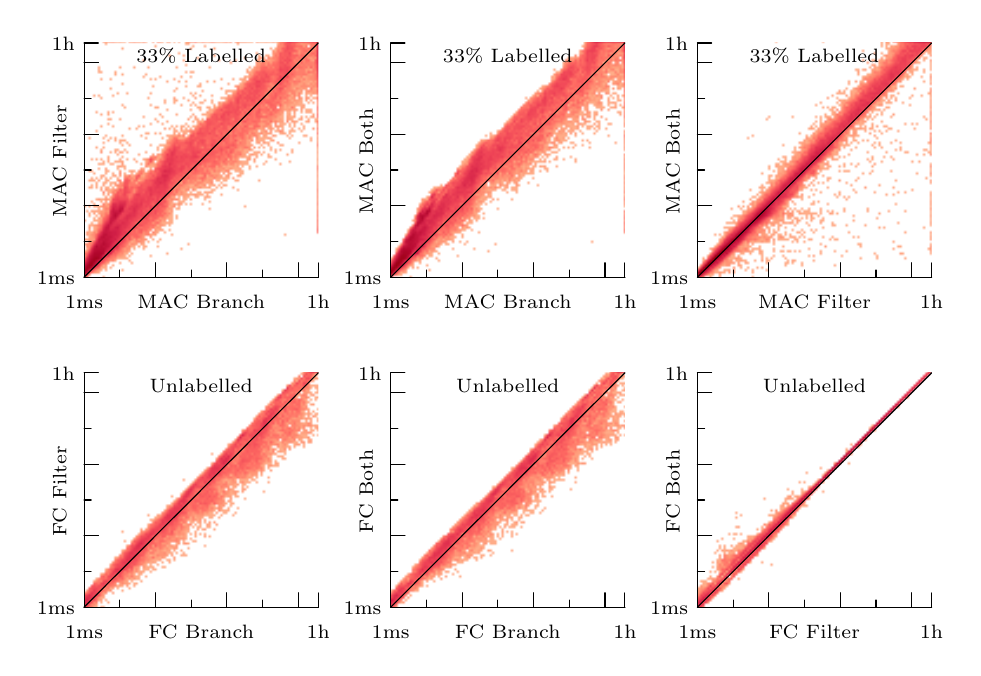
\begin{tikzpicture}[gnuplot]
%% generated with GNUPLOT 5.0p0 (Lua 5.2; terminal rev. 99, script rev. 100)
%% Tue 19 Apr 2016 16:47:19 AEST
\tikzset{every node/.append style={font={\scriptsize}}}
% \path (0.000,0.000) rectangle (11.684,8.382);
\gpcolor{color=gp lt color border}
\gpsetlinetype{gp lt border}
\gpsetdashtype{gp dt solid}
\gpsetlinewidth{1.00}
\draw[gp path] (0.368,7.897)--(0.368,4.923)--(3.342,4.923);
\node[gp node center,rotate=-270] at (0.066,6.410) {MAC Filter};
\node[gp node center] at (1.855,4.614) {MAC Branch};
\begin{scope}
\clip (0.368,7.897) rectangle (3.342,4.923);
\def\gprawrgbimagedata{%
  ffffffffffffffffffffffffffffffffffffffffffffffffffffffff9576ffac88ff9f7dff9576ff8c72ff9f7dffac88%
  ff9f7dffac88ffac88ffffffff9f7dff9f7dff8c72ff9f7dff9f7dffac88ff8c72ffac88ffffffffffffff9f7dffffff%
  ff8c72ff9576ffac88ffffffff9f7dff9f7dffffffffac88ffffffff9f7dffffffffffffffac88ff9f7dff8c72ff9576%
  ff7367ffac88ffac88ff8c72ff9f7dffac88ff9f7dff846eff9576ffac88ffac88ffac88ff9f7dff8c72ffac88ff8c72%
  ffffffff9576ff9f7dff9f7dff9f7dff9f7dffac88ffac88ffac88ffffffff9576ffac88ffac88ffac88ff9f7dffac88%
  ffac88ff9576ffac88ffac88ff846eff6b63ff6b63ee4156e43551e73952f04557ed4155f85a5df24a59f34e5af34e5a%
  f34d59f14958eb3e54ef44578b0000ffffffffffffffffffffffffffffffffffffffffffffffffffffffffffffffac88%
  ffffffffffffffffffffffffffffffffffffffffffffffffffffffffffffffffffffffffffffffffffffffffffffffff%
  ffffffffffffffffffffffffffffffffffffffffffffffffffffffffffffffffffffffffffffffffffffffffffffffff%
  ffffffffac88ffac88ffffffffffffffffffffffffffffffffffffffffffffffffffffffffffffffffffffffffffffff%
  ffffffffffffffffffffffffffffffffffffffffffffac88ffffffffffffffffffffffffffffffffffffffffffffffff%
  ffffffffffffffffffffffffffffffffffffffffffffffffffac88ff846eff846efa5e5ff7585df7585dfe6862fd6561%
  ff846eff8c72ff9f7dff9576ff9576ff8c72ff7e6cff7869ff7367cf1d45ffffffffffffffffffffffffffffffffffff%
  ffffffffffffffffffffffffffffffffffffffffffffffffffffffffffffffffffffffffffffffffffffffffffffffff%
  ffffffffffffffffffffffffffffffffffffffffffffffffffffffffac88ffffffffffffffffffffffffffffffffffff%
  ffffffffffffffffffffffffffffffffffffffffffffffffffffffffac88ffffffffffffffffffffffffffac88ffffff%
  ffffffffffffffffffffffffffffffffffffffffffffffffffffffffffffffffffffffffffffffffffffffffffffffff%
  ffffffffffffffffffffffffffffffffffffffffffffffffffffffffffffffffffffffffffffffff8c72ff8c72ff846e%
  ff6b63f34e5af7565cf95c5efc6260ff6f65ff7367ff6f65ff9f7dff7869ffffffff7e6cff846eff846ecf1d44ffffff%
  ffffffffffffffffffffffffffffffffffffffffffffffffffffffffffffffffffffffffffffffffffffffffffffffff%
  ffac88ffffffffffffffffffffffffffffffffffffffffffffffffffffffffffffffffffffffffffffffffffffffffff%
  ffffffffffffffffffffffffffffffffffffffffffffffffffffffffffffffffffffffffffffffffac88ffffffffffff%
  ffffffffffffffffffffffffffffffffffffffffffffac88ffffffffffffffffffffffffffffffffffffffffffffffff%
  ffffffffffffffffffffffffffffffffffffffffffffffffffffffffffffffffffffffffffffffffffffffffffffac88%
  ffffffffac88ff8c72ff846efc6260fa5e5ff24b59f6545cf6545cff7367ff8c72ff7e6cff7869ff7367ff846eff7367%
  ff7869ff846eff8c72d11e46ffffffffffffffffffffffffffffffffffffffffffffffffffffffffffffffffffffffff%
  ffffffffffffffffffffffffffffffffffffffffffffffffffffffffffffffffffffffffffffffffffffffffffffffff%
  ffffffffffffffffffffffffffffffffffffffffffffffffffffffffffffffffffffffffffffffffffffffffffffffff%
  ffffffffffffffffffffffffffffffffffffffffffffffffffffffffffffffffffffffffffffffffffffffffffffffff%
  ffffffffffffffffffffffffffffffffffffffffffffffffffffffffffffffffffffffffffffffffffffffffffffffff%
  ffffffffffffffffffffffffffffffff9576ffac88ff7869ff846eff6b63f5535bf7565cf95c5ef95c5ef95c5eff6b63%
  ff9576ff7e6cff6f65fe6862ff846eff846eff8c72ff6f65d32048ffffffffffffffffffffffffffffffffffffffffff%
  ffffffffffffffffffffffffffffffffffffffffffffffffffffffffffffffffffffffffffffffffffffffffffffffff%
  ffffffffffffffffffffffffffffffffffffffffffffffffffffffffffffffffffffffffffffffffffffffffffffffff%
  ffffffffffffffac88ffffffffffffffffffffffffffffffffffffffffffffffffffffffffffffffffffffffffffffff%
  ffffffffffffffffffffffffffffffffffffffffffffffffffffffffffffffffffffffffffffffffffffffffffffffff%
  ffffffffffffffffffffac88ffffffffffffffffffffffffffffffffffffff9576ff8c72ff846ef95c5efb605ff85a5d%
  f85a5df24a59ff6b63ff8c72ff7e6cff9576ff7869ff7869ff8c72ff9576ff7367fe6862ff7869cf1d45ffffffffffff%
  ffffffffffffffffffffffffffffffffffffffffffffffffffffffffffffffffffffffffffffffffffffffffffffffff%
  ffffffffffffffffffffffffffffffffffffffffffffffffffffffffffffffffffffffffffffffffffffffffffffffff%
  ffffffffffffffffffffac88ffffffffffffffffffffffffffffffffac88ffffffffffffffffffffffffffffffffffff%
  ffffffffffffffffffffffffffffffffffffffac88ffffffffffffffffffffffffffffffffffffffffffffffffffffff%
  ffffffffffffffffffffffffffffffffffffffffffffffffffffffffac88ffffffffffffffac88ffac88ffffffff9f7d%
  ff7869ff846ef7585dfc6260f85a5df95c5ef6545cfc6260fc6260fc6260ff7e6cfe6862ff6f65ff8c72ff7e6cff7869%
  ff846efe6862d42248ffffffffffffffffffffffffffffffffffffffffffffffffffffffffffffffffffffffffffffff%
  ffffffffffffffffffffffffffffffffffffffffffffffffffffffffffffffffffffffffffffffffffffffffffffffff%
  ffffffffffffffffffffffffffffffffffffffffffffffffffffffffffffffffffffffffffffffffffffffffffffffff%
  ffffffffffffffffffffffffffac88ffffffffffffffffffffffffffffffffffffffffffffffffffffffffffffffffff%
  ffffffffffffffffffffffffffffffffffffffffffffffffffac88ffffffffffffffffffffffffffffffff9f7dff9f7d%
  ff9f7dffffffff7e6cff9f7dff846eff846eff7367f95c5ef7565cfc6260f4505af95c5efe6862fe6862ff846eff6f65%
  ff7869ff7367ff7367ff9576ff9f7dff8c72ff9576d01e46ffffffffffffffffffffffffffffffffffffffffffffffff%
  ffffffffffffffffffffffffffffffffffffffffffffffffffffffffffffffffffffffffffffffffffffffffffffffff%
  ffffffffffffffac88ffffffffffffffffffffffffffffffffffffffffffffffffffffffffffffffffffffffffffffff%
  ffffffffffffffffffffac88ffffffffffffffffffffffffffffffffffffffffffffffffffffffffffffffffffffffff%
  ffffffffffffffac88ffffffffffffffffffffffffffffffffffffffac88ffffffffffffffffffffffffffffffffffff%
  ffffffffffffffac88ff9f7dffffffffac88ff8c72ffac88ff9f7dff9576ff846eff7367f7585dfb605ff34e5af6545c%
  f24b59fc6260ff846eff7367ff846eff7869ff8c72ff6f65ff6b63ff9576ff9f7dfb605fda294bffffffffffffffffff%
  ffffffffffffffffffffffffffffffffffffffffffffffffffffffffffffffffffffffffffffffffffffffffffffffff%
  ffffffffffffffffffffffffffffffffffffffffffffffffffffffffffffffffffffffffffffffffffffffffffffffff%
  ffffffffffffffffffffffffffffffffffffffffffffffffffffffffffffffffffffffffffffffffffffffffffffffff%
  ffffffffffffffffffffffffffffffffffffffffffffffffffffffffffffffffffffffffff9f7dffffffffffffffffff%
  ffffffffffffffffffffffffffffffffffffffffffff9576ff9f7dff8c72ff7869ff9576ff7e6cff9f7dff7367ff7367%
  fe6862f5535bf4505afd6561f34d59fc6260fd6561ff7869ff8c72ff9576fe6862ff846eff7869ff7e6cff7e6cff846e%
  fb605fdc2c4cffffffffffffffffffffffffffffffffffffffffffffffffffffffffffffffffffffffffffffffffffff%
  ffffffffffffffffffffffffffffffffffffffffffffffffffffffffffffffffffffffffffffffffffffffffffffffff%
  ffffffffffffffffffffffffffffffffffffffffffffffffffffffffffffffffffffffffffffffffffffffac88ffffff%
  ffffffffffffffffffffffffffffffffffffffffffffffffffffffffffffffffffffffffffffffffffffffffffffffff%
  ffffffffffffffffffffffffffffffffffffffffffffffffffffffffffffffffffffffffff9576ff9576ff7e6cff7869%
  ff9576ff7367ff7e6cff6b63ff6b63fd6561f85a5df7565cf34d59f85a5dfa5e5fff6b63ff6b63ff7e6cff7367ff846e%
  ff7869ff846eff7e6cff7e6cff846eff6b63e0314fffffffffffffffffffffffffffffffffffffffffffffac88ffffff%
  ffffffffffffffffffffffffffffffffffffffffffffac88ffffffffffffffffffffffffffffffffac88ffffffffffff%
  ffffffffffffffffffffac88ffffffffffffffffffffffffffffffffffffffffffffffffffffffffffffffffffffac88%
  ffffffffffffffffffffffffffffffffffffffffffffffffffffffffffffffffffffffffffffffffac88ffffffffffff%
  ffffffffffffffffffffffffffffffffffffffffffffffffffffffffffffffffffffffffffffffffffffffac88ffffff%
  ff9f7dff8c72ff8c72ff6f65fe6862fd6561ff7e6cff6f65ff846efe6862fe6862f34d59f6545cf34e5af24b59f5515b%
  ff6b63fd6561ff7869ff6f65ff7367ff7e6cff7869ff9576fd6561ff8c72ff6b63e0314fffffffffffffffffffffffff%
  ffffffffffffffffffffac88ffffffffffffffffffffffffffffffffffffffffffffffffffffffffffffffffffffffff%
  ffffffffffffffffffffffffffffffffffffffffffffffffffffffffffffffffffffffffffffffffffffffffffffffff%
  ffffffffffffffffffffffffffffffffffffffffffffffffffffffffffffffffffffffffffffffffffffffffffffffff%
  ffffffffffffffffffffffffffffffffffffffffffffffffffffffffffffffffffffffffffffffffffffffffffffffff%
  ffffffffffffffac88ffffffffac88ff9576ff8c72ff8c72fe6862fd6561ff6b63ff6b63ff6f65ff6b63fe6862fa5e5f%
  ef4457f24a59f34e5af04757f95c5eff6f65ff7869ff9576ff846eff7e6cff7e6cff9f7dff9576ffac88ff7e6cff7869%
  e1314fffffffffffffffffffffffffffffffffffffffffffffac88ffac88ffffffffffffffffffffffffffffffffac88%
  ffffffffffffffffffffffffffffffffffffffffffffffffffffffffffffffffffffffffffffffffffffffffffffffff%
  ffffffffffffffffffffffffffffffffffffffffffffffffffffffffffffffffffffffffffffffffac88ffffffffac88%
  ffac88ffffffffffffffffffffffffffffffffffffffffffffffffffffffffffffffffffffffffffffffffffffffffff%
  ffffffffffffffffffffffffffffffffffffffffffff9f7dffac88ff9f7dff846efd6561fd6561f95c5ef7565cfb605f%
  fd6561fd6561fa5e5fff6b63fd6561f4505af5535bf4505af34d59fe6862ff7367ff7367ff7e6cff7e6cff7e6cff7e6c%
  ff9576ff6f65ff7e6cff7e6cff8c72e63852ffffffffffffffffffffffffffffffffffffffffffffffffffffffffffff%
  ffffffffffffffffffffffffffac88ffffffffffffffac88ffffffffffffffffffffffffffffffffffffffffffffffff%
  ffffffffac88ffffffffffffffffffffffffffffffffffffffffffffffffffffffffffffffffffffffffffffffffffff%
  ffffffffffffffffffffffffffffffffffffffffffffffffffffffffffffffffffffffffffffffffffffffffffffffff%
  ffffffffffffffffffffffffffffffffffffffffffffffffffffffffffffffffffffffffffffffff9576ff9f7dff7367%
  ff6b63f85a5dfa5e5ff85a5df4505afc6260f95c5efc6260fc6260f85a5df95c5ef7585df4505afa5e5fff6f65fc6260%
  ff7367ff7e6cff7e6cff7e6cff7869ff7e6cff9576ff9f7dff8c72ff7e6ced4155ffffffffffffffffffffffffffffff%
  ffffffffffffffffffffffffffffffffffffffffffffffffffffffffffffffffffffffffffffffffffffffffffffffff%
  ffffffffffffffffffffffffffffffffac88ffffffffffffffffffffffffffffffffffffffac88ffffffffffffffffff%
  ffffffffffffffffffffffffffffffffac88ffffffffffffffffffffac88ffffffffffffffffffffffffffffffffffff%
  ffffffffffffffffffffffffffffffffffffffffffffffffffffffffffffffffffffffffffffffffffffffffffffffff%
  ff9f7dffac88ff9f7dff7e6cfb605ff6545cfd6561f7565cf95c5ef34e5af5535bff6b63ff7869ff6b63fd6561ee4256%
  f7585df4505af24a59fe6862ff7869ff7869ff9576ff9576ff846effac88ff9f7dff9576ff8c72ff8c72ff7e6cef4356%
  ffffffffffffffffffffffffffffffffffffffffffffffffffac88ffffffffffffffffffffac88ffffffffffffffffff%
  ffffffffffffffffffffffffffffffffffffffffffffffffffffffffffffffffffffffffffffffffac88ffffffffac88%
  ffffffffffffffffffffffffffffffffffffffffffffac88ffffffffffffffffffffffffffffffffffffffffffffffff%
  ffffffffffffffffffffffffffffffffffffffffffffffffffffffffffffffffffffac88ffffffffffffffffffffffff%
  ffac88ffffffffffffffac88ffac88ff9f7dffffffff7367fc6260f4505af7565cfa5e5ff5515bf4505afa5e5ff85a5d%
  fd6561ff7367ff6b63f5515bf5515bf14958fb605fff6f65ff6f65ff7e6cffac88ff8c72ff8c72ff9f7dff7e6cff9f7d%
  ff9576ff8c72ff8c72ff7e6cf4505affffffffffffffffffffffffffffffffffffffffffffffffffffffffffffffffff%
  ffffffffffffffffffffffffffffffffffffffffffffffffffffffffffffffffffffffffffffffffffffffffffffffff%
  ffffffffffffffffffffffffffffffffffffffffffffffffffffffffac88ffffffffffffffffffffffffffac88ffffff%
  ffffffffac88ffffffffffffffffffffffffffffffffffffffffffffffffffac88ffffffffffffffac88ffffffffffff%
  ffffffffffffffffffffffffffffffffffffffffffffffffffffffffac88ffac88ff7e6cff7367fc6260f7585def4356%
  ef4356f6545cf34d59f7565cf5535bfe6862ff6b63fa5e5ffb605ff6545cfa5e5fff6b63fb605fff846eff846eff7367%
  ff7e6cff7869ff9576ff9f7dff9f7dff9f7dffac88ff9576ff9f7df34e5affffffffffffffffffffffffffffffffffff%
  ffffffffffffffffffffffffffffffffffffffffffffffffffffffffffffffffffffac88ffffffffffffffffffffffff%
  ffffffffffffffffffffffffffffffffffffffffffffffffffffffffffffffffffffffffffffffffffffffffffffffff%
  ffffffffffffffffffffffffffffffffffffffffffffffffffffffffffffffffffffffffffac88ffffffffffffffffff%
  ffffffffffffffffffffffffffffffffffffffffffffffffffac88ffffffffffffffffffffffffffac88ff9f7dff7367%
  fb605ff7585df7585df4505af24b59f34d59f5515bf95c5eff6b63ff7869ff8c72ff7367ff6b63fa5e5ff5515bfd6561%
  ff7869ff6f65ff7367ff9576ff846eff846eff9f7dff9f7dff8c72ff9f7dffac88ff8c72ff9f7dff8c72f6545cffffff%
  ffffffffffffffffffffffffffffffffffffffffffffffffffffffffffffffffffffffffffffffffffffffffffffffff%
  ffffffffffffffffffffffffffffffffffffffffffffffffffffffffffffffffffffffffffffffffac88ffffffffffff%
  ffffffffffffffffffffffffffffffffffffffffffffffffffffffffffffffffffffac88ffffffffffffffffffffffff%
  ffac88ffac88ffffffffffffffffffffffffffffffffffffffffffffffffffffffffffffffffffffffffffffffffffff%
  ff9f7dff8c72ff9f7dff9576ff7869fa5e5ff5515bf7585df85a5def4457f04757f7565cf7565cfd6561ff6f65ff7e6c%
  ff9576ff6b63ff6b63fe6862fd6561fb605fff7869ff7e6cff9576ff9576ff9f7dff9f7dff8c72ff8c72ff8c72ff8c72%
  ff9f7dff8c72ff9576f5515bffffffffffffffffffffffffffffffffffffffffffffffffffffffffffffffffffffffff%
  ffac88ffffffffffffffffffffffffffffffffffffffffffffffffffffffffffffffffffffffffffffffffffffffffff%
  ffffffffffffffffffffffffffffffffffffffffffffffffffffffffffffffffffffffffffac88ffffffffffffffffff%
  ffffffffffffffffffffffffffffffffffffffffffffffffffffffffffffffffffffffffffffffffffffffffffffac88%
  ffffffffffffffffffffffffffffffffffffff7869ff9576ff846ef7565cf85a5df95c5ef24b59fa5e5ff4505af7565c%
  f7565cf95c5efd6561ff8c72ff7e6cff7e6cfd6561fc6260f5515bf95c5eff8c72ff7e6cff846eff9576ffac88ff846e%
  ff9576ff9f7dff9576ff9f7dffffffff7e6cff9f7dffac88ff6b63ffffffffffffffffffffffffffffffffffffffffff%
  ffffffffffffffffffffffffffffffffffffffffffffffffffffffffffffffffffffffffffffffffffffffffffffffff%
  ffffffffffffffffffffffffffffffffffffffffffffffffffffffffffffffffffffffffffffffffffffffffffffffff%
  ffac88ffffffffffffffffffffffffffffffffffffffffffffffffffffffffffffffffffffac88ffffffffffffffffff%
  ffffffffffffffffffffffffffffffffffffffac88ff9f7dffac88ffac88ff9f7dff6f65fe6862f7585dfd6561f95c5e%
  f5515bfa5e5ff34e5af34e5af5515bfa5e5ffc6260ff6b63ff7869ff9576fc6260ff7869fd6561f95c5eff7869ff7869%
  ff846eff846eff846eff8c72ff9f7dffac88ff9576ffffffff9f7dff8c72ff9576ff9f7dff9f7dfc6260ffffffffffff%
  ffffffffffffffffffffffffffffffffffffffffffffffffffffffffffffffffffffffffffffffffac88ffffffffffff%
  ffffffffac88ffffffffffffffffffffffffffffffffffffffffffffffffffffffffac88ffffffffffffffffffffffff%
  ffffffffffffffffffffffffffffffffffffffffffffffffffffffffffffffffffffffffffac88ffffffffac88ffffff%
  ffffffffffffffffffffffffffffffffffffffffffffffffffffffffffffffffffffac88ffffffffffffff9576ff846e%
  f85a5dff6b63f7565cf7565cfc6260f4505af5515bf6545cf34e5afb605ffa5e5ffd6561ff846eff846eff6f65ff7367%
  fa5e5ffe6862ff6b63ff7367ff7869ff8c72ffac88ff846eff846effac88ff846effac88ffffffff9f7dffac88ffac88%
  ff9576ff9f7dff7367ffffffffffffffffffffffffffffffffac88ffffffffac88ffffffffffffffffffffffffffffff%
  ffac88ffffffffffffffffffffffffffffffffffffffffffffffffffffffffffffffffffffffffffffffffffffffffff%
  ffffffffffffffffffffffffffffffffffffffffffffffffffffffffffffffffffffffffffffffffffffffffffffffff%
  ffffffffffffffac88ffffffffffffffac88ffffffffffffffffffffffffffac88ffffffffffffffffffffffffffffff%
  ffffffff9576ffac88ff7e6cff6f65fa5e5ff34e5af95c5efc6260f34e5af7565cf95c5ef34e5afb605ff5515bfc6260%
  fe6862ff9576ff7869fe6862ff6b63f85a5dff6f65ff7869ff7869ff846eff7869ff8c72ffac88ff846effac88ff846e%
  ffffffffffffffac88ffffffffac88ffffffffffffff9576ffffffffffffffffffffffffffffffffffffffffffffffff%
  ffac88ffffffffffffffffffffffffffffffffffffffffffffffffffffffffffffffffffffffffffffffffffffffffff%
  ffffffffffffffffffffffffffac88ffffffffffffffffffffffffffffffffffffffffffffffffffffffffffffff9f7d%
  ffffffffffffffffffffac88ffffffffffffffffffffffffff9f7dffffffffffffffffffffffffffffffffffffffffff%
  ffffffffffffffffffffac88ffac88ff9f7dff8c72ff846eff7869f95c5ef34e5af4505af95c5ef34e5af5535bf34d59%
  f6545cf5535bf5515bfc6260ff6f65fe6862ff846eff846efe6862fb605ffb605fff846efb605fff7e6cff7367ff8c72%
  ffac88ff9576ff9576ffffffff8c72ff9f7dffffffff9576ff9576ffffffffac88ffac88fe6862ffffffffffffffffff%
  ffffffffffffffffffffffffffffffffffffffffffffffffffffffffffffffffffffffffffffffffffffffffffffffff%
  ffffffffffffffffffffffffffffffffffffffffffffffffffffffffffffffffffffffffffffffffffffffffffffffff%
  ffac88ffffffffffffffffffffac88ffac88ffffffffffffffffffffffffffac88ffffffffffffffffffffffffffffff%
  ffffffffac88ffffffffffffffac88ffffffffffffffffffffffffffffffffac88ff7869ff6b63ff7e6cf7585def4356%
  fb605ff85a5dfd6561f4505af95c5ef24a59f4505afe6862f7585dff6b63fd6561ff6b63fe6862ff6b63fd6561ff7869%
  ff7869ff7869ff8c72ff9f7dff846eff9576ffac88ff9576ff9f7dff9f7dffac88ffffffff9f7dffffffffac88ffffff%
  ffffffff7e6cffffffffffffffffffffffffffffffffffffffffffffffffffffffffffffffffffffffffffffffffffff%
  ffffffffffffffffffffffffffffffffffffffffffffffffffffffffffffffffffffffffffffffffffffffffffffffff%
  ffffffffffffffffffffffffffffffffac88ffffffffffffffffffffac88ffffffffffffffffffffffffffffffffffff%
  ffffffffac88ffffffffffffffac88ffac88ffffffffffffffffffffac88ffffffffffffff9576ffac88ff846eff846e%
  ff6f65f5535bfd6561f7585df04757f95c5ef7585df7585df95c5efc6260f7585df7585dff6b63fc6260fc6260ff7869%
  fb605ffa5e5ffd6561ff7367ff6f65fe6862ff7869ff9576ff846eff8c72ff9576ff9576ffac88ff9f7dffac88ffac88%
  ffffffffffffffac88ffffffffac88ffffffff8c72ffffffffffffffffffffffffffffffffffffffffffffffffffffff%
  ffffffffffffffffffffffffffffffffffffffffffffffffffac88ffffffffffffffffffffffffffffffffffffffffff%
  ffffffffffffffffffffffffffac88ffffffffffffffffffffffffffffffffffffffffffffffffffffffffffffffffff%
  ffffffffac88ffffffffffffffffffffac88ffffffffac88ffffffffffffffffffffffffffffffffffffffffffffac88%
  ffffffff9f7dff8c72fe6862fb605ff5535bf5535bf85a5df95c5ef5535bfd6561f6545cf34e5af7585df85a5df95c5e%
  fc6260fe6862fd6561ff7e6cff6f65ff9f7dff7367fb605ffd6561ff6f65ff9576fd6561ff8c72ffac88ff9576ff9f7d%
  ffac88ff9f7dffac88ffac88ffac88ff9f7dffffffffffffffffffffffffffffffff8c72ffffffffffffffffffffffff%
  ffffffffffffffffffffffffffffffffffffffffffffffffffffffffffffffffffffffffffffffffffffffac88ffffff%
  ffffffffffffffffffffffffffffffffffffffffffffffffffffffffffffffffffffac88ffac88ffffffffffffffffff%
  ffffffffffffffffffffffffffffffffffffffffffffffffffffffffffffffffffffffffffffffffac88ffac88ffffff%
  ffffffffac88ffac88ffffffff9f7dffac88ff7869ff7367f95c5ef5515bf4505af7565cf6545cf85a5df24b59f7585d%
  fa5e5ff34e5afd6561fd6561ff7e6cf95c5eff7367ff6b63ff7e6cff7e6cff6f65ff8c72fe6862ff6b63fd6561ffffff%
  ff846eff9576ffac88ff9f7dffac88ff7869ff9f7dffffffffffffff9f7dffac88ffffffffffffffffffffffffffffff%
  fe6862ffffffffffffffffffffffffffffffffffffffffffffffffffffffffffffffffffffffffffffffffffffffffff%
  ffffffffffffffffffffffffffffffffffffffffffffffffffffffffffffffffffffffffffffffffffffffffffffffff%
  ffffffffffffffffffffffffffffffffac88ffffffffffffffffffffffffffffffffffffffffffffffffffffffffac88%
  ffffffffffffffffffffac88ffffffffffffffffffffac88ffac88ff9576ff6f65fd6561f34e5afd6561f95c5ef5535b%
  f7585df5515bf4505af34e5aff6b63f85a5dff7367fc6260fe6862fb605fff7367ff6f65f7585dff6b63ff7367ff6f65%
  fd6561ff9576fb605fff7367ff6f65ff846eff9576ff9f7dff9f7dff9576ffac88ff9f7dff9f7dffffffff9f7dffffff%
  ffac88ffac88ffac88ffffffffffffff6f65ffffffffffffffffffffffffffffffffffffffac88ffffffffffffffffff%
  ffffffffac88ffffffffac88ffffffffffffffffffffffffffffffffffffffffffffffffffffffffffffffffffffffff%
  ffffffffffffffffffffffffffffffffffffffffffffffffffffffffffffffffffffffffffffffffffffffffffffffff%
  ffffffffffffffffffffffffffffffffffffffffffffffffffffffffffffffffffff9f7dffac88ffac88ff7869fe6862%
  fd6561fd6561f6545cf14958f24b59f34d59f6545cf34d59f85a5df5535bff7367f85a5dff7869fc6260ff6b63ff7869%
  fa5e5ff7585dff846eff7869ff7367ff7e6cff6b63ff7e6cff6f65ff846eff9576ff9576ffffffffac88ffac88ffffff%
  ff9f7dffffffffffffffac88ffffffffac88ffac88ffac88ffffffffffffff846effffffffffffffffffffffffffffff%
  ffffffffffffffffffffac88ffffffffffffffac88ffffffffffffffffffffffffffffffffffffffffffffffffffffff%
  ffffffffffffffffffffffffffffffffffffffffffffffffffffffffffffffffffffffffffac88ffffffffffffffffff%
  ffffffffffffffffffffac88ffffffffffffffffffffffffffffffffffffffac88ffffffffffffffffffffac88ffac88%
  ffac88ff9576ff7367f7565cf85a5dfb605ff7565cf04557f7585df14958fa5e5ff85a5df6545cf4505afc6260ff6b63%
  fd6561fd6561fa5e5fff6f65ff7367f95c5efe6862ff7869ff9f7dff846eff7367fd6561ff7869ff8c72ff9576ff9576%
  ffac88ffffffffac88ff9f7dffffffffac88ffffffffffffffffffffffffffffffffffffffffffffac88fffffffe6862%
  ffffffffffffffffffffffffffffffffffffffffffffffffffffffffffffffffffffffffffffffffffffffffffffffff%
  ffffffffffffffffffffffffffffffffffffffffffffffffffffffffffffffac88ffffffffffffffffffffffffffffff%
  ffffffffffffffac88ffffffffffffffffffffffffffffffffffffffffffffffffffffffffffffffffffffac88ffffff%
  ff9f7dffffffffffffffffffffffffffac88ff8c72f7585df95c5ef5535bfe6862ef4457f34d59f7585df7585df85a5d%
  f95c5ef7565cfa5e5fff6b63ff6f65ff6b63ff6f65ff7367ff6b63ff7869fc6260fb605ffd6561ff6b63fe6862ff7e6c%
  ff846eff8c72ff846eff9f7dffac88ffac88ffffffff9f7dffac88ffac88ff9f7dffffffffffffffac88ffffffffac88%
  ffffffffac88ff9f7dffffffff6f65ffffffffffffffffffffffffffffffffffffffffffffffffffffffffffffffffff%
  ffac88ffac88ffffffffffffffffffffac88ffffffffffffffffffffffffffffffffffffffffffffffffffffffffffff%
  ffffffffffffffffffffffffffac88ffffffffffffffffffffffffffffffffffffffffffffffffffffffffffffffffff%
  ffffffffffffff9f7dffffffffffffffac88ffac88ffffffffac88fffffff95c5efa5e5ffa5e5ff85a5df6545cf7565c%
  f5535bf24b59f6545cf5535bfc6260ff7e6cf6545cf85a5dfe6862ff7367ff7869fc6260ff6f65ff6f65ff7869ff7367%
  ff6b63ff9f7dff9576ff8c72ff846eff846eff9576ff9f7dffac88ff9f7dffac88ffffffff9f7dff9f7dffac88ffffff%
  ffffffffac88ff9f7dffffffffffffffac88ffffffffffffffac88ffac88ffffffffffffffffffffffffffffffffffff%
  ffffffffffffffffffffffffffffffffffffffffffffffffffffffffffffffffffffffffffffffffffffffffffffffff%
  ffffffffffffffffffffffffffffffffffffffffffffffffffffffffffffffac88ffffffffffffffffffffac88ffffff%
  ffffffffffffffffffffffffffffffffffffffffffffffffffffffffac88ffffffff9f7dff9f7dffac88ff6b63f7585d%
  f7565cf7585dfa5e5ff85a5dff6f65fb605ff6545cf85a5df85a5dfd6561fa5e5ff7585dfc6260ff7e6cfd6561f6545c%
  ff6f65ff7869ff6b63fd6561ff6b63ff7367ff8c72ff7e6cff846eff9576ff6b63ff9f7dff846eff9f7dff9f7dff9f7d%
  ffffffff8c72ffffffff9f7dff9f7dffac88ffffffffffffffffffffac88ff9f7dffffffffffffffac88ff7367ffffff%
  ffffffffffffffffffffffffffffffffffffffffffffffffffffffffffffffac88ffffffffffffffffffffffffffffff%
  ffffffffffffffffffffffffffffffffffffffffffffffffffffffffffffffffffffffffffac88ffffffffffffffffff%
  ffffffffac88ffffffffffffffffffffffffffffffffffffffffffffffffffffffffac88ffffffffffffffffffffffff%
  ffac88ff6f65ff7869ff7367f7565cf5515bf7585df85a5dfc6260f95c5ef24a59f7565cfa5e5ff6545cf7585dfb605f%
  ff6b63fc6260ff8c72ff7367ff7e6cff6f65ff6f65ff7e6cff7869ff6f65ff9576ff9f7dff9f7dff846eff7e6cffac88%
  ffffffff8c72ffffffffac88ffac88ffac88ffffffffac88ffffffffac88ffffffffffffffac88ffffffffffffffffff%
  ffffffffffffffffffff8c72ffffffffffffffffffffffffffffffffffffffffffffffffffac88ffffffffffffffffff%
  ffffffffac88ffffffffffffffffffffffffffffffffffffffffffffffffffffffffffffffac88ffffffffac88ffffff%
  ffffffffffffffffffffffffffffffffffffffffffffffffffffffffffffffac88ffffffffac88ffffffffac88ffac88%
  ffffffffac88ffffffffac88ffac88ff846eff846efd6561fd6561f5535bf95c5efc6260fb605ff85a5df7585dff6b63%
  f7585dfa5e5fff7367ff6b63fb605ffe6862ff846eff7367ff7e6cf95c5eff6b63ff9576ff9576fe6862fe6862ff6f65%
  ff9f7dff8c72ff8c72ff9f7dff9576ffffffff9576ff9f7dff9f7dffac88ffffffffffffffac88ffffffffac88ffffff%
  ffffffffffffffac88ffffffffffffffffffffffffffffffff9576ffffffffffffffffffffffffffffffffffffffffff%
  ffffffffffffffffffffffffffffffffffffffffffffffffffffffffffffffffffffffffffffffffac88ffffffffffff%
  ffac88ffffffffffffffffffffffffffffffffffffffffffffffffffffffffffffffffffff9f7dffffffffac88ffffff%
  ffac88ffffffffffffff9f7dffffffffac88ffffffffac88ffffffff846eff7e6cf7565cf85a5df85a5df6545cf95c5e%
  fc6260f34e5af95c5efe6862fb605ff7585df85a5dff7869ff7e6cfe6862fe6862ff7e6cff7869fe6862ff7869ff7367%
  ff7367ff7869ff6f65ff9576ff9f7dff9f7dff9576ffffffffac88ff9576ffac88ffffffff9f7dffffffffac88ffffff%
  ffffffffffffffac88ffffffffffffffac88ffffffffac88ffffffffffffffffffff9f7dffffffff6f65ffffffffffff%
  ffffffffffffffffffffffffffac88ffffffffffffffffffffffffffffffffffffffffffffffffffffffffffffffffff%
  ffffffffffffffffffffffffffffffffffffffffffffffffffffffffffffffffffffffffffffffffffffffffffffffff%
  ffffffffffffffffffffffffffffffffac88ff9f7dffffffffac88ffac88ffac88ff9576ff846eff7e6cff7e6cfd6561%
  f5535bfb605ff85a5df6545cfd6561f7565cf7585dff6f65f95c5efc6260fd6561fd6561fc6260ff7869fc6260ff7367%
  ff7367ff7e6cff6b63ff6b63ff7367ff8c72ff8c72ff9f7dff9576ffffffffac88ff9f7dff8c72ffffffff9576ffffff%
  ffac88ffac88ff846eff9f7dffffffffffffffac88ffac88ffac88ffffffffffffffac88ffffffffffffffffffffffff%
  ffffffffffffff9576ffffffffffffffffffffffffffffffffffffffffffffffffffffffffffffffffffffffffffffff%
  ffffffffffffffffffffffffffffffffffffffffffffffffffffffffffffffffffffffffffffffffffffffac88ffac88%
  ffffffffffffffac88ffffffffac88ffffffffffffffffffffffffffffffff9f7dffffffff9f7dffffffff9f7dffac88%
  ffffffff8c72fc6260ff6b63f34d59f34e5af4505af7565cf85a5df34d59f95c5ef7585dff7367ff6b63f6545cff6f65%
  fd6561ff7869ff846efe6862ff7e6cff7367fe6862ff6b63ff7e6cff7367ff9f7dff7e6cff846eff9f7dff9f7dff8c72%
  ffac88ff9f7dff9f7dff9f7dffffffffffffffffffffac88ff9f7dffac88ffffffffac88ffffffffffffffffffffffff%
  ffffffffffffffffffffffffffffffffffffffffffff6f65ffffffffffffffffffffffffffffffffffffffffffffffff%
  ffffffffffffffac88ffffffffffffffffffffffffffffffffffffffac88ffffffffffffffffffffffffffffffffffff%
  ffffffffac88ffffffffffffffffffffffffffffffffffffffffffffffffffffffffffffffac88ffac88ff9f7dff9f7d%
  ff9f7dff846eff9f7dff7e6cffffffffac88f6545cf5535bff6b63f85a5df7585df6545cf7585dfc6260fc6260fb605f%
  f95c5ef5535bfe6862fc6260fe6862ff846efc6260ff7367fd6561fa5e5fff7869ff6b63ff6b63ff846eff9f7dff846e%
  ff9576ff846eff8c72ffac88ffffffff9f7dffac88ffffffffffffff9576ffac88ffffffffffffffffffffffffffac88%
  ffffffffac88ffffffffffffffffffffffffffac88ffac88ffffffffffffffffffffffffffac88ffffffffffffffffff%
  ffac88ffffffffffffffffffffffffffffffffac88ffffffffffffffac88ffffffffac88ffffffffffffffffffffffff%
  ffffffffffffffffffffffffffffffffffffffffffffffffffac88ffffffffffffffffffffffffffffffffffffffac88%
  ffffffffffffffac88ff9f7dff7367ff7869ffac88ffac88ff9f7dff8c72ff6b63f7565cfb605ff7565cf7565cf95c5e%
  f95c5efd6561fd6561fc6260f95c5efd6561fe6862fa5e5ffc6260f85a5dfa5e5ffe6862ff7e6cfe6862ff7e6cff846e%
  ff7e6cff6b63ff846eff9576ff7e6cffac88ffffffff8c72ffac88ffac88ffac88ffac88ff9576ffac88ffffffffffff%
  ffffffffffffffffffffffffffffffffac88ffffffffffffffffffffffffffffffffffffffffffffffffffac88ffffff%
  ffffffff9576ffffffffffffffffffffffffffffffffffffffffffffffffffffffffffffffffffffac88ffffffffffff%
  ffac88ffffffffac88ffac88ffac88ffffffffffffffffffffffffffffffffffffffffffffffffffffffffffffffffff%
  ffffffffffffffffffffffffffffffffffffffac88ff9f7dff846eff6f65fa5e5fff6f65ff7869ff7869fc6260fb605f%
  f5535bf4505af7585dfc6260f4505af24b59f6545cff6b63fd6561f7585df5535bfb605ffe6862fc6260f7585dfe6862%
  ff6b63ff7e6cff7367f95c5eff7e6cff9576ff846eff846eff9f7dffac88ff8c72ffffffff9f7dffac88ffac88ffac88%
  ffffffffffffffac88ff9f7dffffffffffffffffffffffffffffffffffffffffffffffffffffffffffffffffffffffff%
  ffffffffffffffffffffac88ffffffffffffff9f7dffffffffffffffffffffffffffffffffffffffffffffffffffffff%
  ffac88ffffffffffffffffffffffffffffffffffffffac88ffffffffffffffac88ffffffffffffffffffffffffffffff%
  ffffffffffffffffffffffffffffffffffffffffffffffffffffffffffffffffffff9576ff846eff7869fb605ff95c5e%
  fc6260fb605ffa5e5ff4505af5515bf04757f5535bff6f65f4505af7565cf24b59f85a5dff6f65fd6561f7565cf6545c%
  fc6260ff6b63ff6b63ff7e6cfa5e5fff6b63ff7367fd6561ff7367ff9576ff7367ff846eff846eff9f7dff9f7dffffff%
  ffffffffac88ff9576ffffffff9576ffac88ffac88ffffffffffffffffffff9576ffffffffffffffffffffffffffffff%
  ffffffffffffffffffffac88ffffffffffffffffffffffffffffffffffffffffffff9576ffffffffffffffffffffffff%
  ffffffffffffffffffffffffffffffffffffffffffffffffffffffffffffffffffffffffffffffffac88ffffffffffff%
  ffac88ffffffffffffffffffffffffffffffffffffffffffffffffffac88ffffffffffffffffffffac88ffac88ffac88%
  ff9f7dff8c72fd6561f5535bfe6862f85a5dfb605ffb605ffc6260f5535bf14858f85a5dfd6561f6545cfa5e5ff85a5d%
  f7565cfb605ffb605ff04757f7565cff6b63fe6862ff6f65ff7367ff6b63fc6260fc6260f7585dfe6862ff7e6cff846e%
  ff846eff8c72ff9f7dff9f7dff9f7dffffffffffffffffffffac88ffffffffffffffac88ffffffffffffffffffffffff%
  ffac88ffac88ffffffffffffffffffffffffffffffffffffffffffffffffffffffffffffffffffffffffffffffffffff%
  ff7e6cffffffffffffffffffffffffffffffffffffffac88ffffffffffffffac88ffffffffffffffffffffffffffffff%
  ffffffffffffffffffffffffffffffffffffffffffffffffffffffffffffffffffffffffffffffffffffffffffffffff%
  ffffffffac88ffffffffffffff9f7dff846eff6b63f95c5eef4457f34d59f34e5afd6561fd6561f85a5df4505af34e5a%
  f34d59f7565cf5535bfd6561ff7e6cf7585dfd6561ff6b63f7585dfd6561fd6561fb605ffa5e5ffe6862f95c5ef7565c%
  ff7367ff7367fe6862ff846eff9576ff8c72ff7869ff7e6cff9576ffffffff9f7dffffffffac88ffffffffac88ffffff%
  ffffffffac88ffffffffffffffffffffffffffffffffffffffffffffffffffffffffffffffffffffffffffffffffffff%
  ffffffffffffffffffffffffffffffff9f7dffffffffffffffffffffffffffffffffffffffffffffffffffac88ffffff%
  ffffffffffffffffffffffffffac88ffac88ffffffffffffffac88ffffffffffffffffffffffffffffffffffffffffff%
  ffffffffffffffffffffffffffffffffffffffac88ffffffffac88ff9576fd6561f34d59f5515bea3d54f14958f7585d%
  fa5e5ff85a5df34e5af5515bf34e5af24a59f4505af5515bf6545cf6545cf85a5df7585df5535bfb605ffc6260fe6862%
  fb605ff5515bfd6561ff6b63ff7e6cfd6561fe6862ff8c72ff9576ff9f7dff9576ffac88ffac88ff8c72ffac88ffffff%
  ffffffffffffffffffffffffffffffffffffffac88ffffffffac88ffffffffac88ffffffffffffffffffffffffffac88%
  ffffffffffffffffffffffffffffffffffffffffffffffffffffffffffffffac88ffffffffffffffffffffffffffffff%
  ffffffffffffffffffff9576ffffffffffffffffffffac88ffffffffac88ffffffff9f7dffac88ffffffffac88ffffff%
  ffffffffffffffffffffffffffffffffffffffac88ffffffffffffffffffffffffffffffffffffff9f7dff6b63fd6561%
  f34e5ae73a52ea3d54f34d59f4505af34e5af7565cf5515bf95c5ef4505aef4356f14958ef4356f24b59fd6561fc6260%
  f7585dfa5e5ff85a5df95c5ef95c5eff6b63fa5e5fff7869fb605fff7869f85a5dff7367ff8c72ff7e6cff846eff9f7d%
  ffac88ff9f7dffffffffffffffac88ffac88ff9f7dffffffffac88ffffffffffffffffffffffffffac88ffffffffffff%
  ffffffffffffffffffffffffffac88ffffffffffffffffffffffffffffffffffffffffffffffffffffffffffffff9f7d%
  ffffffffffffffffffffffffffffffffffffffffffffffffffffffffffffffffffffffffffffffffffffffffffffac88%
  ffffffffffffffffffffffffffffffffffffffffffffffffffac88ffffffffffffffffffffffffffffffff9f7dffffff%
  ff9576ff9f7dff7869fe6862ec3f55f14958e43651ed4155f4505af34d59f4505af04757f24a59f34e5af5535bef4457%
  ee4156f7565cf95c5ef7565cf6545cf4505af95c5ef85a5dfb605fff7367ff7367fd6561ff7367ff7367fc6260ff7869%
  ff9576ff7e6cff846eff7869ff9f7dff9f7dffffffffac88ff9576ffac88ffac88ffffffffac88ffffffffffffffac88%
  ffffffffffffffffffffffffffffffffffffffffffffac88ffffffffffffffffffffffffffffffffffffffffffffffff%
  ffffffffffffffffffffffffffac88ffffffffffffffffffffffffffffffffffffffffffffffffffffffffffffffffff%
  ffac88ffffffffffffffffffffffffffffffffac88ffffffffffffffffffffffffffffffffffffffffffffffffffffff%
  ffffffffffffff846eff8c72ff7869ff9f7dffac88ff7e6cf95c5ef14858ee4156ea3d54f04757ec4055f34d59ee4256%
  f24a59ef4356f24b59f04757ec4055e93c53ee4156f7585df6545cf85a5dfe6862fb605ffd6561fc6260fe6862fb605f%
  ff7367ff7367ff846efe6862ff6f65ff8c72ff7e6cff9576ffac88ff9f7dffac88ffac88ff9f7dffffffffffffff9f7d%
  ffffffffffffffffffffffffffac88ffac88ffffffffffffffffffffffffffffffffffffffffffffffffffffffffffff%
  ffffffffffffffffffffffffffffffffffffffffffffffffffffffffac88ffffffffffffffffffffffffffac88ffffff%
  ffac88ffffffffac88ffffffffffffffac88ffffffffffffffffffffffffffac88ffffffffffffffac88ffffffffffff%
  ffac88ffffffffffffffffffffac88ff9f7dff846ef24a59ff6f65ff8c72ffac88ff846eff7e6cf85a5dea3d54e93c53%
  e73a52ed4155f14958f34d59f04757f04757f5515bf4505af14858f14958f5515bf85a5dfd6561f24b59f95c5ef95c5e%
  fd6561ff6b63ff6b63ff846efe6862ff7869ff7869fd6561ffac88ff6f65ff9f7dff8c72ff9f7dffffffffffffffffff%
  ff9f7dff9576ffffffff9f7dffffffffffffffffffffffffffffffffffffffffffffffffffac88ffffffffffffffffff%
  ffffffffffffffffffffffffffffffffffffffffffffffffffffffffffffffffffffffffffffffffffffff9f7dffffff%
  ffffffffffffffffffffffffffffffffffffffffffffffffffac88ffffffffac88ffffffffffffffac88ffac88ffac88%
  ff9f7dffffffffffffffffffffffffffffffffac88ffffffffffffffffffffac88ff8c72f7565cff9576ffffffff9f7d%
  fe6862f7585def4356ea3d54ea3d54e93c53ef4356ef4356f14858f04757f34d59f34d59f4505af34d59f24a59f34d59%
  f6545cfd6561f95c5efb605ffd6561ff6b63ff6b63fa5e5ffe6862ff7869ff846efd6561ff7e6cff846eff8c72ff7e6c%
  ff846eff9576ff9f7dffac88ffac88ffac88ffffffffffffffac88ffffffffffffffffffffffffffac88ffffffffffff%
  ffffffffffffffffffffffffffffffffffffffffffffac88ffffffffffffffffffffffffffffffffffffffffffffffff%
  ffffffffffffffffffffac88ffffffffffffffffffffffffffffffffffffffffffffac88ffac88ffac88ffffffffffff%
  ffac88ffac88ffffffffffffffffffff9f7dffffffffffffffffffffffffffffffffffffffffffffac88ffffffff9f7d%
  ff7367ff9f7dff9f7dff9f7dff7367ff6f65f5535bee4156f14858e1324fea3d54ef4457f24a59f34e5af34e5af6545c%
  f14858f34d59f4505af7585df85a5df7565cf5515bff6f65ff6b63ff7e6cff846eff6f65fe6862ff6b63ff6f65ff9576%
  ff846eff7869ff9f7dff846eff8c72ffac88ff9f7dffac88ffac88ffac88ffac88ffffffffffffffffffffffffffffff%
  ffffffffac88ffffffffffffffffffffffffffffffffffffffac88ffffffffffffffffffffffffffffffffffffffffff%
  ffffffffffffffffffffffffffffffffffffffffffffffffffac88ffffffffffffffffffffffffffffffffffffffffff%
  ffffffffffffffffffffffffffffffffffffffffffffffffffac88ff9f7dffac88ffac88ffffffffffffffffffffffff%
  ffffffffffffffffffffffffff8c72ffac88ffac88ffac88ff9576ff6f65fa5e5fee4156e83a53eb3e54e63852ef4457%
  ec4055f14858f7565cf04757ef4457f7585df24b59f95c5efc6260f5515bfe6862ff7367ff8c72fe6862ff7e6cff6f65%
  fe6862fe6862ff9f7dff7e6cff8c72ffac88ff9f7dffac88ffac88ff9f7dffac88ff9f7dffffffffac88ffffffffffff%
  ffac88ffffffffffffffac88ffffffffffffffffffffffffffffffffffffffffffffffffffffffffffffffffffffffff%
  ffffffffffffffffffffffffffffffffffffffffffffffffffffffffffffffffffffffffffffffff846effffffffffff%
  ffffffffffffffffffffffffffffffffac88ffffffffffffff9f7dffffffffffffffffffffffffffac88ffffffffffff%
  ffac88ffffffffffffffffffffffffffffffffffffff9f7dffac88ffffffffffffff9f7dfffffffc6260f5515bf04557%
  ec4055e83a53e63852e23450e73a52f04557f14958f14858ed4155f14958f95c5ef7585df5535bf95c5ef6545cff7367%
  ff7367ff6f65ff8c72ff7e6cff9576ff7e6cff846eff9f7dff9576ff9576ff8c72ffac88ff9f7dff9576ffac88ffac88%
  ffac88ff9f7dffffffffffffffffffffac88ffffffffffffffffffffffffffffffffffffffffffffffffffffffffffff%
  ffffffffffffffffffffffffffffffffffffffffffffffffffffffffffffffffffffffffffffffffffffffffffffffff%
  ffffffffffffff7e6cffffffffffffffffffffac88ffac88ffffffffffffffffffffffffffffffffac88ffac88ffffff%
  ffffffffffffffffffff9f7dffffffffffffffffffffac88ff9f7dffac88ffffffff9576ff7e6cff8c72ffffffffac88%
  ff6f65ff7e6cf7585dfb605fee4156e63852d9284bdf2f4ee0314fe63852ea3d54f24a59f24a59f04557f85a5dfb605f%
  f6545cfa5e5fff7367fb605ffe6862ff7367ff7367ff8c72ff6f65ff8c72ff9f7dff7869ff9576ff8c72ff9f7dffac88%
  ff846eff8c72ffffffffffffffac88ffac88ffac88ffac88ffffffffffffffffffffffffffffffffffffffffffffffff%
  ffffffffffffffffffffffffffffffffffffffffffffffffffffffffffffffffffffffffffffffffffffffffffffffff%
  ffffffffffffffffffffffffffffffffffffffffffff9576ffffffffffffffffffffffffffffffffac88ffffffffffff%
  ffffffffffffffac88ffffffffffffffac88ffffffffffffff8c72ffffffffac88ffffffffffffffac88ffffffffac88%
  ff846eff7367ff9f7dff9576ff7e6cfc6260ff6f65fd6561f5515bf14958e53751e43651e33550e23450ea3d54ec4055%
  f14958f7565cf7585df85a5df7585dff7869ff7869fe6862ff6b63ff7367ff7e6cff7367ff6f65ff7e6cff7869ff9f7d%
  ff9f7dff9f7dff9f7dffffffff9576ffffffff9f7dffac88ffffffffffffffffffffac88ffac88ffffffffffffffffff%
  ffffffffffffffffffffffffffffffffffffffffffffffffffffffffffffffffffffffffffffffffffffffffffffffff%
  ffffffffffffffffffffffffffffffffffffffffffffffffffffffffffffffffffffffffff9f7dffffffffffffffffff%
  ffffffffffffffffffffffffffffffffac88ff9f7dffffffffffffffffffffac88ff9f7dffffffff9f7dffffffff9576%
  ff9f7dff7367ffac88ff9f7dff6b63f5535bff9f7dffac88ff846eff7367ff6f65f6545cfc6260f14858ee4156de2d4d%
  da294bde2d4dea3d54f04557f14958f95c5ef85a5df6545cff6b63ff7e6cff6f65ff7367ff7e6cff7e6cff9576ff9f7d%
  ff9576fb605fffac88ff8c72ff7e6cff9576ff8c72ff9f7dff9f7dffffffff9f7dff9576ffffffffffffffffffff9f7d%
  ffac88ffffffffffffffffffffffffffffffffffffffffffffffffffffffffffffffffffffffffffffffffffffffffff%
  ffffffffffffffffffffffffffffffffffffffffffffffffffffffffffffffffffffffffffffffffffffffffffffffff%
  ffffffff9576ffffffffffffffffffffffffffac88ffffffffac88ffffffffac88ffffffffac88ffffffffac88ffffff%
  ffffffffac88ffffffffffffff846eff6f65ff8c72ff8c72ff9f7df7585dff7e6cff9576ff9576ff7e6cff6f65fb605f%
  fb605ff24a59e23450e43651e33450df2f4ee23450ea3d54f04757fb605ff85a5dfc6260ff6f65fd6561ff6f65fc6260%
  ff7e6cff7869ff7e6cff8c72ff7869ff6b63ff7869ff9f7dff9f7dff9f7dff7e6cff9f7dff9f7dffac88ffac88ffac88%
  ffac88ffffffff9f7dffffffffffffffffffffffffffffffffffffffffffffffffffffffffffffffffffffffffffffff%
  ffffffffffffffffffffffffffffffffffffffffffffffffffffffffffffffffffffffffffffffffffffffffffffffff%
  ffffffffffffffffffffffffffffffffffffff9f7dffffffffffffffffffffac88ffac88ffac88ffffffff9f7dffffff%
  ffffffffac88ffac88ffffffffffffffffffff9f7dff7e6cfffffffa5e5ff7585dfd6561ff9f7dff7869ff7367ffac88%
  ff9576ff7e6cf7585df85a5df34e5af04557ea3d54e1324fe53651e43651de2e4de73a52ee4256fb605ff7585dfd6561%
  fc6260ff7869ff7367ff7869ff9576ff7e6cff8c72ff846eff9f7dff9f7dff7869ff9576ff9f7dff9576ff9576ffffff%
  ffac88ffac88ffffffffac88ffac88ffffffffffffffffffffac88ffac88ffffffffffffffffffffffffffffffffffff%
  ffffffffffffffac88ffffffffffffffffffffffffffffffffffffffffffffffffffffffffffffffffffffffffffffff%
  ffffffffffffffffffffffffffffffffffffffffffffffffffffffffffffffffffff9f7dffffffffffffffffffffffff%
  ffffffffffffffac88ffffffffffffffac88ffac88ffffffffac88ffac88ff9f7dffffffff8c72ff9576f7565cf7565c%
  ff7367ff7e6cff7e6cffac88ff6b63ff6b63fb605ff7565cf7585df7565cf04757e53651e63852de2e4de43551e43651%
  ed4155f34e5af4505af95c5efd6561ff846eff9f7dfd6561ff7e6cff8c72ff846eff8c72ff9f7dff846eff846eff9576%
  ffac88ff9f7dff9f7dff8c72ffffffffffffffffffffac88ffffffffffffffffffffffffffffffffffffffffffffffff%
  ffffffffffffffffffffffffffffffffffffffffffffffffffffffffffffffffffffffffffffffffffffffffffffffff%
  ffffffffffffffffffffffffffffffffffffffffffffffffffffffffffffffffffffffffffffffffffffffffffffffff%
  ff9576ffffffffffffffffffffffffffac88ffffffffac88ffffffffffffff9f7dffffffffffffffac88ffffffff9f7d%
  ff8c72ff8c72ff7869f7565cf85a5dff7e6cff7869ff7869ff7367ff7869f5535bf85a5df85a5df6545cf5515bee4256%
  ec3f55e43551e93c53eb3e54e53751ee4156f85a5df7585dfd6561ff8c72ff7869ff7367ff8c72ff9576ff9f7dffac88%
  ffac88ff846eff9576ffac88ff9f7dff8c72ffffffffac88ffac88ff9f7dffffffffac88ffffffff9f7dffac88ffffff%
  ffffffffffffffffffffffffffffffffffffffffffffffffffffffffffffffffffffffffffffffffffffffffffffffff%
  ffffffffffffffffffffffffffffffffffffffffffffffffffffffffffffffffffffffffffffffffffffffffffffffff%
  ffffffffffffffffffffffffffffffff9576ffffffffffffffffffffac88ffac88ffffffffac88ffffffffac88ffffff%
  ffac88ffac88ffffffffac88ffffffff9f7dff846eff9576ef4457f4505aff6f65fb605fff6f65fc6260f4505af5515b%
  f95c5ef6545cee4156e93c53ee4156e83a53e73952eb3e54ec4055ea3d54ee4156f6545cfc6260ff8c72ff846eff7e6c%
  ff9576ff9576ff9f7dff9576ffac88ff9f7dffac88ff9f7dff8c72ffac88ffac88ffac88ff9f7dffffffffffffffac88%
  ffffffffac88ffffffffffffffffffffffffffac88ffffffffffffffffffffffffffffffffffffffffffffffffffffff%
  ffffffffffffffffffffffffffffffffffffffffffffffffffffffffffffffffffffffffffffffffffffffffffffffff%
  ffffffffffffffffffffffffffffffffffffffffffffffffffffffffffffff9576ffffffffffffffffffffffffffffff%
  ffffffffffffffffffff9f7dffffffff9576ffac88ffac88ff9f7dff846eff846ef6545cfc6260f14858f5515bfb605f%
  fe6862ff8c72ff6b63f5515bf34e5af5515bf34e5aec4055e43551ed4155ea3d54ef4356ec3f55ec4055ec4055f34e5a%
  fc6260fb605fff846eff6f65ff846eff9f7dffac88ff8c72ff8c72ffffffff846effac88ffffffffffffffffffffffff%
  ffffffffffffffac88ffac88ffffffffffffffffffffffffffffffffffffffffffffffffffffffffac88ffffffffffff%
  ffffffffffffffffffffffffffffffffffffffffffffffffffffffffffffffffffffffffffffffffffffffffffffffff%
  ffffffffffffffffffffffffffffffffffffffffffffffffffffffffffffffffffffffffffffffffffffffffffff846e%
  ffffffffffffffffffffffffffffffffffffffffffffffffffffffff846effffffffac88ffac88ff846eff9576f85a5d%
  fb605ffa5e5ff04557f34d59f7585dff6f65ff8c72fa5e5ff34d59f34e5af85a5def4356f04757e83a53eb3e54ed4155%
  ea3d54e93c53ee4156f04557f4505af5535bff6b63ff8c72ff6f65ff9f7dff8c72ff9f7dffac88ffffffffac88ffffff%
  ffffffffac88ffac88ffffffff9f7dffac88ff9f7dffac88ffffffffffffffffffffffffffffffffffffffffffffffff%
  ffffffffffffffffffffffffffffffffffffffffffffffffffffffffffffffffffffffffffffffffffffffffffffffff%
  ffffffffffffffffffffffffffffffffffffffffffffffffffffffffffffffffffffffffffffffffffffffffffffffff%
  ffffffffffffffffffffffffff8c72ffffffffffffffffffffffffffffffffffffffffffffffffffffffffac88ffffff%
  ff9f7dffffffff8c72fc6260f6545cfd6561f5535bef4356fb605fff7367ff7367f7565cea3d54ea3d54f34e5af14958%
  f04557f24a59e23450ef4356f04757ef4356ed4155f14958ec3f55f7565cff6b63ff7e6cff7367ff9f7dff9f7dff9576%
  ff9f7dff9f7dff9f7dffac88ff9f7dff9576ffac88ffac88ffac88ffffffffac88ffffffffffffffffffffffffffffff%
  ffac88ffffffffffffffffffffffffffffffffffffffffffffffffffffffffffffffffffffffffffffffffffffffffff%
  ffffffffffffffffffffffffffffffffffffffffffffffffffffffffffffffffffffffffffffffffffffffffffffffff%
  ffffffffffffffffffffffffffffffffffffffffffffffffffffffff9576ffffffffffffffffffffffffffffffffffff%
  ffffffffffffffffffffffffff9f7dffffffffac88ff7e6cf6545cf24a59f5535bf6545cf34d59f7565cff7869fe6862%
  f14958f04557ee4256ef4457f04557f04757ed4155ed4155f34e5af5515bed4155f24a59f24b59f7565cff6f65ff7869%
  ff9f7dff9f7dffffffffac88ffffffff9f7dffac88ffac88ffffffffffffffac88ffac88ffffffffffffffac88ff9f7d%
  ffac88ffffffffffffffffffffffffffffffffffffffffffffffffffffffffffffffffffffffffffffffffffffffffff%
  ffffffffffffffffffffffffffffffffffffffffffffffffffffffffffffffffffffffffffffffffffffffffffffffff%
  ffffffffffffffffffffffffffffffffffffffffffffffffffffffffffffffffffffffffffffffffffffff8c72ffffff%
  ffffffffffffffffffffffffffffffffac88ff9576ffac88ffac88ff9576ff9f7dffac88f24b59f14858ed4155f14958%
  f24a59f14858f24a59fc6260f6545cee4256eb3e54ef4356ec3f55eb3e54f24b59ec4055f04557ee4256f5515bee4156%
  fb605ff7565cfc6260ff846eff9576ff846eff9576ff846effac88ffffffffac88ffac88ffffffff9f7dffffffffffff%
  ffffffffffffffffffffac88ffffffffffffffffffffffffffffffffffffffffffffffffffffffffffffffffffffffff%
  ffffffffffffffffffffffffffffffffffffffffffffffffffffffffffffffffffffffffffffffffffffffffffffffff%
  ffffffffffffffffffffffffffffffffffffffffffffffffffffffffffffffffffffffffffffffffffffffffffffffff%
  ffffffffffffffffffff9576ffffffffffffffffffffffffffac88ffffffffffffffffffffac88ffffffff9f7dffffff%
  ff7e6cf34e5aef4457ec3f55e53651e53651e33450ef4457f5535bee4156ee4156eb3e54ef4457e83a53ee4256ed4155%
  ee4256f24b59f6545cf34d59ee4256f34e5af85a5df5535bff7367ff9576ff9f7dffffffffffffffac88ffac88ffac88%
  ffffffffffffffffffffffffffffffffffffffffffffffffffffffffffffffac88ffffffffffffffffffffffffffffff%
  ffffffffffffffffffffffffffffffffffffffffffffffffffffffffffffffffffffffffffffffffffffffffffffffff%
  ffffffffffffffffffffffffffffffffffffffffffffffffffffffffffffffffffffffffffffffffffffffffffffffff%
  ffffffffffffffffffffffffffffffffffffffffffffffffff8c72ffffffffffffffffffffffffffffffffac88ffffff%
  ffffffffffffff7e6cffac88ff9576ff6b63df304edf2f4ee63852dc2c4ddb2b4cdd2d4df04757f34d59f04557e83a53%
  e63852e93c53e43651f24b59f14858ee4256f5515bfc6260f5535bf24b59f24a59f7565cff6f65ff7367ff9576ffac88%
  ff9576ffac88ff9576ff9f7dffffffffac88ffffffffac88ffffffffffffffffffffffffffac88ffffffffffffffffff%
  ffffffffffffffffffffffffffffffffffffffffffffffffffffffffffffffffffffffffffffffffffffffffffffffff%
  ffffffffffffffffffffffffffffffffffffffffffffffffffffffffffffffffffffffffffffffffffffffffffffffff%
  ffffffffffffffffffffffffffffffffffffffffffffffffffffffffffffffffffffffffffffffff846effffffffac88%
  ffffffffac88ffffffffac88ffac88ffac88ff9f7dff8c72ff9576ff9f7df34e5ad9284bd9284be0304ed11f46d11f46%
  e2324ff24b59ee4156e63852e53751e1314fe73952ea3d54f24b59ee4256f34e5aef4457f7585df5535bf34d59fb605f%
  f7585dfa5e5fff7367ffac88ff9f7dff8c72ffffffffac88ffffffffffffffffffffffffffffffffffffffffffffffff%
  ffffffffffffffffffffffffffffffffffffffffffffffffffffffffffffffffffffffffffffffffffffffffffffffff%
  ffffffffffffffffffffac88ffffffffffffffffffffffffffffffffffffffffffffffffffffffffffffffffffffffff%
  ffffffffffffffffffffffffffffffffffffffffffffffffffffffffffffffffffffffffffffffffffffffffffffffff%
  ffffffffffffff9576ffffffffffffffffffffffffffffffffffffffffffffac88ffffffff9f7dff7e6cff846ef04757%
  ce1c44d72549d8264ac5153dc6163dee4256ef4457e43651e63852dd2d4de53651ea3d54f04557f14958f5515bf85a5d%
  f04557f6545cf7585df7565cfb605fff6b63ff6f65ff9576ff9576ff9f7dffffffffac88ffac88ffffffffffffffffff%
  ffffffffffffffffffffffffffffffffffffffffffffffffffffffffac88ffffffffffffffffffffffffffffffffffff%
  ffffffffffffffffffffffffffffffffffffffffffffffffffffffffffffffffffffffffffffffffffffffffffffffff%
  ffffffffffffffffffffffffffffffffffffffffffffffffffffffffffffffffffffffffffffffffffffffffffffffff%
  ffffffffffffffffffffffffffffffffffffffffffff9576ffffffffffffffac88ffffffff9f7dffac88ff9f7dffac88%
  ff9f7dff9f7dff8c72ff9576de2d4dca1941cc1b43ce1c44be1037d52349ea3d54ea3d54ec3f55e73952de2d4de63852%
  f14958ec4055f7565cf24b59f5515bf34e5af85a5df24b59f85a5dfb605ffd6561ff846eff9576ffac88ff9576ffffff%
  ffffffffffffffffffffffffffffffffffffffffffffffffffffffffffffffffffffffffffffffffffffffffffffffff%
  ffffffffffffffffffffffffffffffffffffffffffffffffffffffffffffffffffffffffffffffffffffffffffffffff%
  ffffffffffffffffffffffffffffffffffffffffffffffffffffffffffffffffffffffffffffffffffffffffffffffff%
  ffffffffffffffffffffffffffffffffffffffffffffffffffffffffffffffffffffffffff846effffffffffffffffff%
  ffac88ffffffff9f7dffffffffac88ff9576ff9576ff7869ff846ed9284bca1941c01239c7173ed32048ee4156ed4155%
  ea3d54e33450e33550e23350e93c53ef4457ef4457f04757f95c5ef14858f5535bf85a5df34e5aff6b63fb605fff7869%
  ff6f65ff8c72ff8c72ffac88ffffffffffffffffffffffffffffffffffffffffffffffffffffffffffffffffffffffff%
  ffffffffffffffffffffffffffffffffffffffffffffffffffffffffffffffffffffffffffffffffffffffffffffffff%
  ffffffffffffffffffffffffffffffffffffffffffffffffffffffffffffffffffffffffffffffffffffffffffffffff%
  ffffffffffffffffffffffffffffffffffffffffffffffffffffffffffffffffffffffffffffffffffffffffffffffff%
  ffffffff846effffffffffffffffffffac88ffffffffffffffac88ffffffff8c72ff9576ff6b63f7565cda294bc7173f%
  bb0e35cf1d44e93c53ef4356ea3d54de2e4dde2e4ee33450e33450ec3f55f24b59ee4156f34d59f7585df34e5afa5e5f%
  f85a5dfb605ffb605ffe6862fe6862ff8c72ff8c72ffac88ffac88ffffffffac88ffffffffffffffffffffffffffffff%
  ffffffffffffffffffffffffffffffffffffffffffffffffffffffffffffffffffffffffffffffffffffffffffffffff%
  ffffffffffffffffffffffffffffffffffffffffffffffffffffffffffffffffffffffffffffffffffffffffffffffff%
  ffffffffffffffffffffffffffffffffffffffffffffffffffffffffffffffffffffffffffffffffffffffffffffffff%
  ffffffffffffffffffffffffffffffffffffff7e6cffffffffffffffffffffffffffffffffac88ffffffff9f7dffac88%
  ff6f65fa5e5ff04757cf1d45c8183fc7173ee1314fee4256ea3d54e1324fdd2d4de33550e73a52ed4155f04757f24b59%
  f85a5df4505af14858f95c5eff6f65fc6260fa5e5fff6f65ff9576ff8c72ff8c72ffac88ffac88ffac88ffffffffac88%
  ffffffffffffffffffffffffffffffffffffffffffffffffffffffffffffffffffffffffffffffffffffffffffffffff%
  ffffffffffffffffffffffffffffffffffffffffffffffffffffffffffffffffffffffffffffffffffffffffffffffff%
  ffffffffffffffffffffffffffffffffffffffffffffffffffffffffffffffffffffffffffffffffffffffffffffffff%
  ffffffffffffffffffffffffffffffffffffffffffffffffffffffffffffffffffff8c72ffac88ff9f7dffffffffffff%
  ffffffffac88ffac88ffac88ff9f7dfd6561f4505ae73a52ca1941ce1c44db2a4ce83a53e23450e23450e33550e1314f%
  ea3d54eb3e54f04757f24b59fc6260f5535bf95c5ef95c5ef85a5dfe6862fb605fff7e6cff9576ff7e6cff9f7dff9576%
  ffffffffac88ffac88ffffffffffffffffffffffffffffffffffffffffffffffffffffffffffffffffffffffffffffff%
  ffffffffffffffffffffffffffffffffffffffffffffffffffffffffffffffffffffffffffffffffffffffffffffffff%
  ffffffffffffffffffffffffffffffffffffffffffffffffffffffffffffffffffffffffffffffffffffffffffffffff%
  ffffffffffffffffffffffffffffffffffffffffffffffffffffffffffffffffffffffffffffffffffffffffffffffff%
  ff7869ffffffffffffffffffffffffffac88ffffffffffffff9f7dff9576f85a5de63852db2a4cc7173edb2a4ce0314f%
  e2324fe53651dc2b4cdf304ee43551e83b53f14858f4505afe6862f7565cfb605ff85a5df85a5dfe6862ff6b63ff9576%
  ff7869fe6862ff9576ffac88ffac88ff9f7dffac88ffac88ffffffffffffffffffffffffffffffffffffffffffffffff%
  ffffffffffffffffffffffffffffffffffffffffffffffffffffffffffffffffffffffffffffffffffffffffffffffff%
  ffffffffffffffffffffffffffffffffffffffffffffffffffffffffffffffffffffffffffffffffffffffffffffffff%
  ffffffffffffffffffffffffffffffffffffffffffffffffffffffffffffffffffffffffffffffffffffffffffffffff%
  ffffffffffffffffffffffffffffffff7e6cffffffffffffffffffffac88ffac88ff9f7dff9576ff7e6cff7367ee4156%
  d9284bc91840d52349df2f4edf304eda294bdb2a4ce23350e1324fe53751ed4155f24a59f4505aff6b63f6545cf4505a%
  fa5e5ffe6862ff6b63ff7367ff6f65ff7e6cffac88ff9576ff9576ffac88ffffffffac88ffffffffffffffffffffffff%
  ffffffffffffffffffffffffffffffffffffffffffffffffffffffffffffffffffffffffffffffffffffffffffffffff%
  ffffffffffffffffffffffffffffffffffffffffffffffffffffffffffffffffffffffffffffffffffffffffffffffff%
  ffffffffffffffffffffffffffffffffffffffffffffffffffffffffffffffffffffffffffffffffffffffffffffffff%
  ffffffffffffffffffffffffffffffffffffffffffffffffffffffffffffff7e6cffac88ffffffffffffff9576ffffff%
  ffac88ff9f7dff846efd6561e0314fca1940c8173fdc2b4cdc2c4cd42248cf1d45dd2d4de43651e33450eb3e54ef4356%
  f6545cf24a59f5535bfe6862ff7367fe6862ff6b63ff6f65ff846eff7869ff9f7dff9576ff9f7dffffffffffffffffff%
  ffffffffffffffffffffffffffffffffffffffffffffffffffffffffffffffffffffffffffffffffffffffffffffffff%
  ffffffffffffffffffffffffffffffffffffffffffffffffffffffffffffffffffffffffffffffffffffffffffffffff%
  ffffffffffffffffffffffffffffffffffffffffffffffffffffffffffffffffffffffffffffffffffffffffffffffff%
  ffffffffffffffffffffffffffffffffffffffffffffffffffffffffffffffffffffffffffffffffffffffffffff7367%
  ffffffffffffffffffffac88ffffffffac88ff9576fe6862f7565cd52349c8183fcd1b43d9274bd52349d52349d62449%
  de2d4de33550eb3e54f14958f14858fa5e5ffb605fff7869fc6260f85a5dff6f65ff6b63ff846eff8c72ffffffff9576%
  ffac88ff9f7dff9f7dffffffffffffffac88ffffffffffffffffffffffffffffffffffffffffffffffffffffffffffff%
  ffffffffffffffffffffffffffffffffffffffffffffffffffffffffffffffffffffffffffffffffffffffffffffffff%
  ffffffffffffffffffffffffffffffffffffffffffffffffffffffffffffffffffffffffffffffffffffffffffffffff%
  ffffffffffffffffffffffffffffffffffffffffffffffffffffffffffffffffffffffffffffffffffffffffffffffff%
  fffffffffffffffffffffffffd6561ffffffffffffff9f7dffac88ffac88ff8c72ff9576f85a5de1314fcb1a42c91840%
  cc1b42ce1c44d11e46d01e46d62449db2a4ce53751e53751ef4356f24b59ff6b63fd6561ff7367fd6561fa5e5fff8c72%
  ff7e6cff846effffffff846eff9f7dffac88ffffffffffffffac88ffffffffffffffffffffffffffffffffffffffffff%
  ffffffffffffffffffffffffffffffffffffffffffffffffffffffffffffffffffffffffffffffffffffffffffffffff%
  ffffffffffffffffffffffffffffffffffffffffffffffffffffffffffffffffffffffffffffffffffffffffffffffff%
  ffffffffffffffffffffffffffffffffffffffffffffffffffffffffffffffffffffffffffffffffffffffffffffffff%
  ffffffffffffffffffffffffffffffffffffffffffffffffffffffff7869ffffffffffffff9f7dffac88ff9576ff8c72%
  fd6561e73a52d7254ac3143bc01239ca1940ce1c44d11e46d22047d62449df2f4ee63852ef4457ed4155fc6260fd6561%
  fd6561fd6561ff7869ff7e6cff9576ff846eff7e6cff9f7dffac88ff9f7dffffffffffffffffffffffffffffffffffff%
  ffac88ffffffffffffffffffffffffffffffffffffffffffffffffffffffffffffffffffffffffffffffffffffffffff%
  ffffffffffffffffffffffffffffffffffffffffffffffffffffffffffffffffffffffffffffffffffffffffffffffff%
  ffffffffffffffffffffffffffffffffffffffffffffffffffffffffffffffffffffffffffffffffffffffffffffffff%
  ffac88ffffffffffffffffffffffffffffffffffffffffffffffffffffffffffffffffffffffffffffffffffffffffff%
  ffffffffffffffac88ff9f7dff8c72f95c5ed9284bc4143cbe1037c8173fc7173ec9183fd11e46d8264ad9284be53751%
  f24b59f34d59f95c5ef95c5eff846eff6b63fd6561ff6b63ff846eff9f7dffffffffffffff9576ffffffffffffffffff%
  ffffffffffffffffffffffffffffffffffffffffffffffffffffffffffffffffffffffffffffffffffffffffffffffff%
  ffffffffffffffffffffffffffffffffffffffffffffffffffffffffffffffffffffffffffffffffffffffffffffffff%
  ffffffffffffffffffffffffffffffffffffffffffffffffffffffffffffffffffffffffffffffffffffffffffffffff%
  ffffffffffffffffffffffffffffffffffffffffffffffffffffffffffffffffffffffffffffffffffffffffffffffff%
  ffffffffffffffffffffffffff9576ff9f7dffac88ff9f7dff9f7dff9f7def4457c7173ec4153cc6163ec3143bc6163d%
  cf1d45d42248d21f47e23450ea3d54eb3e54f34e5aff6f65fa5e5fff7e6cff9f7dff7869ff9f7dff8c72ff9576ff9576%
  ffffffffffffffac88ffffffffffffffac88ffffffffffffffffffffffffffffffffffffffffffffffffffffffffffff%
  ffffffffffffffffffffffffffffffffffffffffffffffffffffffffffffffffffffffffffffffffffffffffffffffff%
  ffffffffffffffffffffffffffffffffffffffffffffffffffffffffffffffffffffffffffffffffffffffffffffffff%
  ffffffffffffffffffffffffffffffffffffffffffffffffffffffffffffffffffffffffffffffffffffffffffffffff%
  ffffffffffffffffffffffffffffffffffffffffffffffffffffffffffffffffffffffffff846eff9576f95c5edc2c4d%
  c7173ec91940bd1037c2143bca1941c91840d32048e1324fe43651f04557f04757f95c5eff6f65ff8c72ffac88ff9f7d%
  ff8c72ff846eff9576ff9f7dffffffffac88ffffffffffffffffffffac88ffffffffffffffffffffffffffffffffffff%
  ffffffffffffffffffffffffffffffffffffffffffffffffffffffffffffffffffffffffffffffffffffffffffffffff%
  ffffffffffffffffffffffffffffffffffffffffffffffffffffffffffffffffffffffffffffffffffffffffffffffff%
  ffffffffffffffffffffffffffffffffffffffffffffffffffffffffffffffffffffffffffffffffffffffffffffffff%
  ffffffffffffffffffffffffffffffffffffffffffffffffffffffffffffffffffffffffffffffffffffff9576ffac88%
  ff8c72ff8c72ff7367e73952cb1a41c7173fc2133ab70b32c01239c4153ccc1b43de2d4de53751e83a53ee4256f85a5d%
  ff6b63ff7e6cffac88ff8c72ff9576ff9f7dffffffff9f7dffac88ffffffffffffffffffffffffffffffffffffffffff%
  ffffffffffffffffffffffffffffffffffffffffffffffffffffffffffffffffffffac88ffffffffffffffffffffffff%
  ffffffffffffffffffffffffffffffffffffffffffffffffffffffffffffffffffffffffffffffffffffffffffffffff%
  ffffffffffffffffffffffffffffffffffffffffffffffffffffffffffffffffffffffffffffffffffffffffffffffff%
  ffffffffffffffffffffffffffffffffffffffffffffffffffffffffffffffffffffffffffffffffffffffffffffffff%
  ffffffffffffffffffffac88ffffffff8c72ff8c72f34d59ce1c44b60b31c2133abb0e34c2133ac01138c4153cd62449%
  e33450dd2d4de73952f85a5dfc6260ff7367ff9576ff8c72ffac88ffac88ffffffff9f7dffffffffac88ffac88ffffff%
  ffffffffffffffffffffac88ffffffffffffffffffffffffffffffffffffffffffffffffffffffffffffffffffffffff%
  ffffffffffffffffffffffffffffffffffffffffffffffffffffffffffffffffffffffffffffffffffffffffffffffff%
  ffffffffffffffffffffffffffffffffffffffffffffffffffffffffffffffffffffffffffffffffffffffffffffffff%
  ffffffffffffffffffffffffffffffffffffffffffffffffffffffffffffffffffffffffffffffffffffffffffffffff%
  ffffffffffffffffffffffffffffffffffffffffffffffffffac88ffffffffac88ff7869dc2c4dc01238bb0e34bb0e34%
  bb0e35b90d33c4143cd32048dd2d4de1314fec4055f14958fc6260ff846eff9f7dff8c72ff9576ffffffffac88ffffff%
  ffffffffffffffac88ffffffffffffffffffffffffffffffffffffffffffffffffffffffffffffffffffffffffffffff%
  ffffffffffffffac88ffffffffffffffffffffffffffffffffffffffffffffffffffffffffffffffffffffffffffffff%
  ffffffffffffffffffffffffffffffffffffffffffffffffffffffffffffffffffffffffffffffffffffffffffffffff%
  ffffffffffffffffffffffffffffffffffffffffffffffffffffffffffffffffffffffffffffffffffffffffffffffff%
  ffffffffffffffffffffffffffffffffffffffffffffffffffffffffffffffffffffffffffffffffffffffac88ff8c72%
  f34e5acf1d45bb0e35b60a31b50930b70b32b80c32cd1b43df2f4ed7254ae53651fb605ffb605fff7367ff846eff9576%
  ff9576ffac88ffffffffffffffffffffffffffffffffffffffffffffffffffffffffffffffffffffffffffffffffffff%
  ffffffffffffffffffffffffffffffffffffffffffffffffffffffffffffffffffffffffffffffffffffffffffffffff%
  ffffffffffffffffffffffffffffffffffffffffffffffffffffffffffffffffffffffffffffffffffffffffffffffff%
  ffffffffffffffffffffffffffffffffffffffffffffffffffffffffffffffffffffffffffffffffffffffffffffffff%
  ffffffffffffffffffffffffffffffffffffffffffffffffffffffffffffffffffffffffffffffffffffffffffffffff%
  ffffffffffffff8c72ff7869fd6561df2f4ec3143bb3082eb0062cb0062cb0062cbb0e35ea3d54d9274bdd2d4dfb605f%
  fc6260ff7869ff8c72ff8c72ffac88ffac88ffffffffac88ffffffffffffffffffffffffffffffffffffffffffffffff%
  ffffffffffffffffffffffffffffffffffffffac88ffffffffffffffffffffffffffffffffffffffffffffffffffffff%
  ffffffffffffffffffffffffffffffffffffffffffffffffffffffffffffffffffffffffffffffffffffffffffffffff%
  ffffffffffffffffffffffffffffffffffffffffffffffffffffffffffffffffffffffffffffffffffffffffffffffff%
  ffffffffffffffffffffffffffffffffffffffffffffffffffffffffffffffffffffffffffffffffffffffffffffffff%
  ffffffffffffffffffffffffffffffffffffffffffffac88ff9576f24a59c91940b90c33af062bad0629ae0629bb0e35%
  db2b4ce73a52ea3d54fe6862ff7367ff7367ff9576ff9576ff9f7dffac88ffffffffac88ffffffffffffffffffffffff%
  ffffffffffffffffffffffffffac88ffffffffffffffffffffffffffffffffffffffffffffffffffffffffffffffffff%
  ffffffffffffffffffffffffffffffffffffffffffffffffffffffffffffffffffffffffffffffffffffffffffffffff%
  ffffffffffffffffffffffffffffffffffffffffffffffffffffffffffffffffffffffffffffffffffffffffffffffff%
  ffffffffffffffffffffffffffffffffffffffffffffffffffffffffffffffffffffffffffffffffffffffffffffffff%
  ffffffffffffffffffffffffffffffffffffffffffffffffffffffffffffffffffffffffff9f7dfe6862db2a4cbf1138%
  b2082ea90524a4041dab0527c2133bf04557f6545cff6b63ff7869ff846eff8c72ffac88ffac88ffac88ffac88ffac88%
  ffffffffffffffffffffffffffffffffffffffffffffffffffffffffffffffffffffffffffffffffffffffffffffffff%
  ffffffffffffffffffffffffffffffffffffffffffffffffffffffffffffffffffffffffffffffffffffffffffffffff%
  ffffffffffffffffffffffffffffffffffffffffffffffffffffffffffffffffffffffffffffffffffffffffffffffff%
  ffffffffffffffffffffffffffffffffffffffffffffffffffffffffffffffffffffffffffffffffffffffffffffffff%
  ffffffffffffffffffffffffffffffffffffffffffffffffffffffffffffffffffffffffffffffffffffffffffffffff%
  ffffffff7e6ced4155cf1d44b60a31ab0526a5041fb60a31cd1b43e93c53f5515bff6b63ff7869ff9576ff846effac88%
  ffffffffffffffffffffffffffffffffac88ffffffffffffffffffffffffffffffffffffffffffffffffffffffffffff%
  ffffffffffffffffffffffffffffffffffffffffffffffffffffffffffffffffffffffffffffffffffffffffffffffff%
  ffffffffffffffffffffffffffffffffffffffffffffffffffffffffffffffffffffffffffffffffffffffffffffffff%
  ffffffffffffffffffffffffffffffffffffffffffffffffffffffffffffffffffffffffffffffffffffffffffffffff%
  ffffffffffffffffffffffffffffffffffffffffffffffffffffffffffffffffffffffffffffffffffffffffffffffff%
  fffffffffffffffffffffffffffffffffffff5515bd9284bc01138ab0526a1031ab2082ec7173edf304ef5535bfd6561%
  ff8c72ff9f7dffffffffffffffffffffffffffac88ffffffffffffffffffffffffffac88ffffffffffffffffffffffff%
  ffffffffffffffffffffffffffffffffffffffffffffffffffffffffffffffffffffffffffffffffffffffffffffffff%
  ffffffffffffffffffffffffffffffffffffffffffffffffffffffffffffffffffffffffffffffffffffffffffffffff%
  ffffffffffffffffffffffffffffffffffffffffffffffffffffffffffffffffffffffffffffffffffffffffffffffff%
  ffffffffffffffffffffffffffffffffffffffffffffffffffffffffffffffffffffffffffffffffffffffffffffffff%
  ffffffffffffffffffffffffffffffffffffffffffffffffffffffffffffffffffe1324fc8173faf062ba00319a5041f%
  c01239da2a4cf14858ff7869ffac88ff9f7dffffffffffffffac88ffffffffffffffffffffffffffffffffffffffffff%
  ffffffffffffffffffffffffffffffffffffffffffffffffffffffffffffffffffffffffffffffffffffffffffffffff%
  ffffffffffffffffffffffffffffffffffffffffffffffffffffffffffffffffffffffffffffffffffffffffffffffff%
  ffffffffffffffffffffffffffffffffffffffffffffffffffffffffffffffffffffffffffffffffffffffffffffffff%
  ffffffffffffffffffffffffffffffffffffffffffffffffffffffffffffffffffffffffffffffffffffffffffffffff%
  ffffffffffffffffffffffffffffffffffffffffffffffffffffffffffffffffffffffffffffffffffffffffffffffff%
  d11f46b80c33a4041da60420c01138e2324ff6545cff6b63ffac88ffac88ffac88ffffffffac88ffffffffffffffffff%
  ffffffffffffffffffffffffffffffffffffffffffffffffffffffffffffffffffffffffffffffffffffffffffffffff%
  ffffffffffffffffffffffffffffffffffffffffffffffffffffffffffffffffffffffffffffffffffffffffffffffff%
  ffffffffffffffffffffffffffffffffffffffffffffffffffffffffffffffffffffffffffffffffffffffffffffffff%
  ffffffffffffffffffffffffffffffffffffffffffffffffffffffffffffffffffffffffffffffffffffffffffffffff%
  ffffffffffffffffffffffffffffffffffffffffffffffffffffffffffffffffffffffffffffffffffffffffffffffff%
  ffffffffffffffffffffffffffffffb40930a60421a70522c6163dee4156fe6862ff8c72ff9f7dffac88ffffffffac88%
  ffffffffffffffffffffffffffffffffffffffac88ffffffffffffffffffffffffffffffffffffffffffffffffffffff%
  ffffffffffffffffffffffffffffffffffffffffffffffffffffffffffffffffffffffffffffffffffffffffffffffff%
  ffffffffffffffffffffffffffffffffffffffffffffffffffffffffffffffffffffffffffffffffffffffffffffffff%
  ffffffffffffffffffffffffffffffffffffffffffffffffffffffffffffffffffffffffffffffffffffffffffffffff%
  ffffffffffffffffffffffffffffffffffffffffffffffffffffffffffffffffffffffffffffffffffffffffffffffff%
  ffffffffffffffffffffffffffffffffffffffffffffffffffffffffffff97020fa00319c11239ef4457ff7367ff9576%
  ff9f7dffac88ffffffffffffffffffffffffffffffffffffffffffffffffffffffffffffffffffffffffffffffffffff%
  ffffffffffffffffffffffffffffffffffffffffffffffffffffffffffffffffffffffffffffffffffffffffffffffff%
  ffffffffffffffffffffffffffffffffffffffffffffffffffffffffffffffffffffffffffffffffffffffffffffffff%
  ffffffffffffffffffffffffffffffffffffffffffffffffffffffffffffffffffffffffffffffffffffffffffffffff%
  ffffffffffffffffffffffffffffffffffffffffffffffffffffffffffffffffffffffffffffffffffffffffffffffff%
  ffffffffffffffffffffffffffffffffffffffffffffffffffffffffffffffffffffffffffffffffffffffffff8d0002%
  bc0f36f14858ff9576ffffffffffffffffffffffffffffffffffffffffffffffffffffffffffffffffffffffffffffff%
  ffffffffffffffffffffffffffffffffffffffffffffffffffffffffffffffffffffffffffffffffffffffffffffffff%
  ffffffffffffffffffffffffffffffffffffffffffffffffffffffffffffffffffffffffffffffffffffffffffffffff%
  ffffffffffffffffffffffffffffffffffffffffffffffffffffffffffffffffffffffffffffffffffffffffffffffff%
  ffffffffffffffffffffffffffffffffffffffffffffffffffffffffffffffffffffffffffffffffffffffffffffffff%
  ffffffffffffffffffffffffffffffffffffffffffffffffffffffffffffffffffffffffffffffffffffffffffffffff%
  ffffffffffffffffffffffff8b0000f5515bff7e6cffffffffffffffffffffffffffffffffffffffac88ffffffffffff%
  ffffffffffffffffffffffffffffffffffffffffffffffffffffffffffffffffffffffffffffffffffffffffffffffff%
  ffffffffffffffffffffffffffffffffffffffffffffffffffffffffffffffffffffffffffffffffffffffffffffffff%
  ffffffffffffffffffffffffffffffffffffffffffffffffffffffffffffffffffffffffffffffffffffffffffffffff%
  ffffffffffffffffffffffffffffffffffffffffffffffffffffffffffffffffffffffffffffffffffffffffffffffff%
  ffffffffffffffffffffffffffffffffffffffffffffffffffffffffffffffffffffffffffffffffffffffffffffffff%
  ffffffffffffffffffffffffffffffffffffffffffffffffffffff}%
\gprawimage{rgb}{0.353}{4.908}{101}{101}{3.004}{3.004}{\gprawrgbimagedata}{}
\end{scope}
\gpcolor{rgb color={0.000,0.000,0.000}}
\draw[gp path] (0.368,4.923)--(0.398,4.953)--(0.428,4.983)--(0.458,5.013)--(0.488,5.043)%
  --(0.518,5.073)--(0.548,5.103)--(0.578,5.133)--(0.608,5.163)--(0.638,5.193)--(0.668,5.223)%
  --(0.698,5.253)--(0.728,5.283)--(0.759,5.314)--(0.789,5.344)--(0.819,5.374)--(0.849,5.404)%
  --(0.879,5.434)--(0.909,5.464)--(0.939,5.494)--(0.969,5.524)--(0.999,5.554)--(1.029,5.584)%
  --(1.059,5.614)--(1.089,5.644)--(1.119,5.674)--(1.149,5.704)--(1.179,5.734)--(1.209,5.764)%
  --(1.239,5.794)--(1.269,5.824)--(1.299,5.854)--(1.329,5.884)--(1.359,5.914)--(1.389,5.944)%
  --(1.419,5.974)--(1.449,6.004)--(1.479,6.034)--(1.510,6.065)--(1.540,6.095)--(1.570,6.125)%
  --(1.600,6.155)--(1.630,6.185)--(1.660,6.215)--(1.690,6.245)--(1.720,6.275)--(1.750,6.305)%
  --(1.780,6.335)--(1.810,6.365)--(1.840,6.395)--(1.870,6.425)--(1.900,6.455)--(1.930,6.485)%
  --(1.960,6.515)--(1.990,6.545)--(2.020,6.575)--(2.050,6.605)--(2.080,6.635)--(2.110,6.665)%
  --(2.140,6.695)--(2.170,6.725)--(2.200,6.755)--(2.231,6.786)--(2.261,6.816)--(2.291,6.846)%
  --(2.321,6.876)--(2.351,6.906)--(2.381,6.936)--(2.411,6.966)--(2.441,6.996)--(2.471,7.026)%
  --(2.501,7.056)--(2.531,7.086)--(2.561,7.116)--(2.591,7.146)--(2.621,7.176)--(2.651,7.206)%
  --(2.681,7.236)--(2.711,7.266)--(2.741,7.296)--(2.771,7.326)--(2.801,7.356)--(2.831,7.386)%
  --(2.861,7.416)--(2.891,7.446)--(2.921,7.476)--(2.951,7.506)--(2.982,7.537)--(3.012,7.567)%
  --(3.042,7.597)--(3.072,7.627)--(3.102,7.657)--(3.132,7.687)--(3.162,7.717)--(3.192,7.747)%
  --(3.222,7.777)--(3.252,7.807)--(3.282,7.837)--(3.312,7.867)--(3.342,7.897);
\gpcolor{color=gp lt color border}
\draw[gp path] (0.368,4.923)--(0.548,4.923);
\node[gp node right] at (0.368,4.923) {1ms};
\draw[gp path] (0.368,5.830)--(0.548,5.830);
\draw[gp path] (0.368,6.737)--(0.548,6.737);
\draw[gp path] (0.368,7.645)--(0.548,7.645);
\draw[gp path] (0.368,7.897)--(0.548,7.897);
\node[gp node right] at (0.368,7.897) {1h~};
\draw[gp path] (0.368,4.923)--(0.548,4.923);
\draw[gp path] (0.368,5.377)--(0.458,5.377);
\draw[gp path] (0.368,5.830)--(0.548,5.830);
\draw[gp path] (0.368,6.284)--(0.458,6.284);
\draw[gp path] (0.368,6.737)--(0.548,6.737);
\draw[gp path] (0.368,7.191)--(0.458,7.191);
\draw[gp path] (0.368,7.645)--(0.548,7.645);
\draw[gp path] (0.368,4.923)--(0.368,5.103);
\node[gp node center] at (0.368,4.615) {1ms};
\draw[gp path] (1.275,4.923)--(1.275,5.103);
\draw[gp path] (2.182,4.923)--(2.182,5.103);
\draw[gp path] (3.090,4.923)--(3.090,5.103);
\draw[gp path] (3.342,4.923)--(3.342,5.103);
\node[gp node center] at (3.342,4.615) {1h~};
\draw[gp path] (0.368,4.923)--(0.368,5.103);
\draw[gp path] (0.822,4.923)--(0.822,5.013);
\draw[gp path] (1.275,4.923)--(1.275,5.103);
\draw[gp path] (1.729,4.923)--(1.729,5.013);
\draw[gp path] (2.182,4.923)--(2.182,5.103);
\draw[gp path] (2.636,4.923)--(2.636,5.013);
\draw[gp path] (3.090,4.923)--(3.090,5.103);
\draw[gp path] (0.368,7.897)--(0.368,4.923)--(3.342,4.923);
\node[gp node center] at (1.855,7.748) {33\% Labelled};
%% coordinates of the plot area
\gpdefrectangularnode{gp plot 1}{\pgfpoint{0.368cm}{4.923cm}}{\pgfpoint{3.342cm}{7.897cm}}
\draw[gp path] (4.262,7.897)--(4.262,4.923)--(7.236,4.923);
\node[gp node center,rotate=-270] at (3.960,6.410) {MAC Both};
\node[gp node center] at (5.749,4.614) {MAC Branch};
\begin{scope}
\clip (4.262,7.897) rectangle (7.236,4.923);
\def\gprawrgbimagedata{%
  ffffffffffffffffffffffffffffffffffffffffffffffffffffffffffffffffffffffffffffffffffffffffffffffff%
  ffffffffffffffffffffffffffffffffffffffffffffffffffffffffffffffffffffffffffffffffffffffffffffffff%
  ffffffffffffffffffffffffffffffffffffffffffffffffffffffffffffffffffffffffffffffffffffffffffffffff%
  ffffffffffffffffffffffffffffffffffffffffffffffffffffffffffffffffffffffffffffffffffffffffffffffff%
  ffffffffffffffffffffffffffffffffffffffffffffffffffffffffffffffffffffffffffffffffffffffffffffffff%
  ffffffffffffffffffffac88ff7869f95c5eee4256d7264ad21f47d42248de2e4edf304ee93c53e33450e33550e2324f%
  e73a52df2f4ed9274bd321488b0000ffffffffffffffffffffffffffffffffffffffffffffffffffffffffffffffffff%
  ffffffffffffffffffffffffffffffffffffffffffffffffffffffffffffffffffffffffffffffffffffffffffffffff%
  ffffffffffffffffffffffffffffffffffffffffffffffffffffffffffffffffffffffffffffffffffffffffffffffff%
  ffffffffffffffffffffffffffffffffffffffffffffffffffffffffffffffffffffffffffffffffffffffffffffffff%
  ffffffffffffffffffffffffffffffffffffffffffffffffffffffffffffffffffffffffffffffffffffffffffffffff%
  ffffffffffffffffffffffffffffffffffffffffffffffffff9f7dfe6862fc6260f6545cf34e5aef4356f85a5dfc6260%
  ff7869ff7e6cff846eff7e6cff7367ff7869ff846eff846eff8c72db2a4cffffffffffffffffffffffffffffffffffff%
  ffffffffffffffffffffffffffffffffffffffffffffffffffffffffffffffffffffffffffffffffffffffffffffffff%
  ffffffffffffffffffffffffffffffffffffffffffffffffffffffffffffffffffffffffffffffffffffffffffffffff%
  ffffffffffffffffffffffffffffffffffffffffffffffffffffffffffffffffffffffffffffffffffffffffffffffff%
  ffffffffffffffffffffffffffffffffffffffffffffffffffffffffffffffffffffffffffffffffffffffffffffffff%
  ffffffffffffffffffffffffffffffffffffffffffffffffffffffffffffffffffffffffffac88ff9576fd6561f95c5e%
  f34d59ea3d54eb3e54f5515bfc6260fe6862ff7869fa5e5fff6f65ff7e6cff8c72ff7e6cff846eff6f65dd2d4dffffff%
  ffffffffffffffffffffffffffffffffffffffffffffffffffffffffffffffffffffffffffffffffffffffffffffffff%
  ffffffffffffffffffffffffffffffffffffffffffffffffffffffffffffffffffffffffffffffffffffffffffffffff%
  ffffffffffffffffffffffffffffffffffffffffffffffffffffffffffffffffffffffffffffffffffffffffffffffff%
  ffffffffffffffffffffffffffffffffffffffffffffffffffffffffffffffffffffffffffffffffffffffffffffffff%
  ffffffffffffffffffffffffffffffffffffffffffffffffffffffffffffffffffffffffffffffffffffffffffffffff%
  ffffffffffffff7367fa5e5ff5535bef4356ee4156f95c5ef7585df95c5eff6f65ff846eff9576ff7e6cff7869ff7e6c%
  ff7e6cff9576ff6f65df304effffffffffffffffffffffffffffffffffffffffffffffffffffffffffffffffffffffff%
  ffffffffffffffffffffffffffffffffffffffffffffffffffffffffffffffffffffffffffffffffffffffffffffffff%
  ffffffffffffffffffffffffffffffffffffffffffffffffffffffffffffffffffffffffffffffffffffffffffffffff%
  ffffffffffffffffffffffffffffffffffffffffffffffffffffffffffffffffffffffffffffffffffffffffffffffff%
  ffffffffffffffffffffffffffffffffffffffffffffffffffffffffffffffffffffffffffffffffffffffffffffffff%
  ffffffffffffffffffffffffffffffff9f7dff7367fd6561f04757ee4256ec4055ef4356f4505afd6561ff7869ff6f65%
  ff7869fe6862fd6561ff7e6cff9576ff8c72ff8c72fe6862de2d4dffffffffffffffffffffffffffffffffffffffffff%
  ffffffffffffffffffffffffffffffffffffffffffffffffffffffffffffffffffffffffffffffffffffffffffffffff%
  ffffffffffffffffffffffffffffffffffffffffffffffffffffffffffffffffffffffffffffffffffffffffffffffff%
  ffffffffffffffffffffffffffffffffffffffffffffffffffffffffffffffffffffffffffffffffffffffffffffffff%
  ffffffffffffffffffffffffffffffffffffffffffffffffffffffffffffffffffffffffffffffffffffffffffffffff%
  ffffffffffffffffffffffffffffffffffffffffffffffffffffffffffffff9f7dff8c72fb605ff04557f4505af04757%
  f5535bf7565cfe6862ff7869ff7367ff846eff7869ff9576ff7869ff7869ff9f7dff9f7dff9576e73952ffffffffffff%
  ffffffffffffffffffffffffffffffffffffffffffffffffffffffffffffffffffffffffffffffffffffffffffffffff%
  ffffffffffffffffffffffffffffffffffffffffffffffffffffffffffffffffffffffffffffffffffffffffffffffff%
  ffffffffffffffffffffffffffffffffffffffffffffffffffffffffffffffffffffffffffffffffffffffffffffffff%
  ffffffffffffffffffffffffffffffffffffffffffffffffffffffffffffffffffffffffffffffffffffffffffffffff%
  ffffffffffffffffffffffffffffffffffffffffffffffffffffffffffffffffffffffffffffffff8c72ffffffff7e6c%
  fd6561fc6260f14958f34d59f24b59f14858f5535bff7367ff7367ff7869ff8c72fc6260ff6b63ff7869ff9576ff9576%
  ff846eff8c72e2324fffffffffffffffffffffffffffffffffffffffffffffffffffffffffffffffffffffffffffffff%
  ffffffffffffffffffffffffffffffffffffffffffffffffffffffffffffffffffffffffffffffffffffffffffffffff%
  ffffffffffffffffffffffffffffffffffffffffffffffffffffffffffffffffffffffffffffffffffffffffffffffff%
  ffffffffffffffffffffffffffffffffffffffffffffffffffffffffffffffffffffffffffffffffffffffffffffffff%
  ffffffffffffffffffffffffffffffffffffffffffffffffffffffffffffffffffffffffffffffffffffffffffffac88%
  ff9f7dff9f7dff9576ff9576ff6f65fe6862f85a5df04757f4505af04757f14958fd6561ff7367ff6b63ff7869ff6f65%
  ff846eff8c72ff9576ff846eff7e6cffffffff7869e83a53ffffffffffffffffffffffffffffffffffffffffffffffff%
  ffffffffffffffffffffffffffffffffffffffffffffffffffffffffffffffffffffffffffffffffffffffffffffffff%
  ffffffffffffffffffffffffffffffffffffffffffffffffffffffffffffffffffffffffffffffffffffffffffffffff%
  ffffffffffffffffffffffffffffffffffffffffffffffffffffffffffffffffffffffffffffffffffffffffffffffff%
  ffffffffffffffffffffffffffffffffffffffffffffffffffffffffffffffffffffffffffffffffffffffffffffffff%
  ffffffffffffffffffff8c72ffac88ff9576ff9576fd6561ff846efa5e5fff6b63f7565cec3f55f6545cf14958f7585d%
  fa5e5fff7869ff7869ff6f65ff9576ffac88ff7869ff9576ff7869ff846eff7869ff9576f24a59ffffffffffffffffff%
  ffffffffffffffffffffffffffffffffffffffffffffffffffffffffffffffffffffffffffffffffffffffffffffffff%
  ffffffffffffffffffffffffffffffffffffffffffffffffffffffffffffffffffffffffffffffffffffffffffffffff%
  ffffffffffffffffffffffffffffffffffffffffffffffffffffffffffffffffffffffffffffffffffffffffffffffff%
  ffffffffffffffffffffffffffffffffffffffffffffffffffffffffffffffffffffffffffffffffffffffffffffffff%
  ffffffffffffffffffffffffffffffffffffffffffff9f7dff8c72ff7e6cfe6862fe6862fb605fff7367fd6561ff6b63%
  fa5e5ff34e5af34e5af5535bf24b59fe6862ff7869ff7367ffac88ff9576ff6f65ff8c72ffffffff9576ff846effffff%
  ff9576f34e5affffffffffffffffffffffffffffffffffffffffffffffffffffffffffffffffffffffffffffffffffff%
  ffffffffffffffffffffffffffffffffffffffffffffffffffffffffffffffffffffffffffffffffffffffffffffffff%
  ffffffffffffffffffffffffffffffffffffffffffffffffffffffffffffffffffffffffffffffffffffffffffffffff%
  ffffffffffffffffffffffffffffffffffffffffffffffffffffffffffffffffffffffffffffffffffffffffffffffff%
  ffffffffffffffffffffffffffffffffffffffffffffffffffffffffffffffffffffffffff9f7dff7869fc6260fa5e5f%
  f7565cfb605fff6f65fa5e5ffd6561fa5e5ff4505af4505afb605ffb605fff6b63ff846eff6f65ff8c72ff846eff846e%
  ff9576ff8c72ff846eff8c72ff9f7dffac88f5515bffffffffffffffffffffffffffffffffffffffffffffffffffffff%
  ffffffffffffffffffffffffffffffffffffffffffffffffffffffffffffffffffffffffffffffffffffffffffffffff%
  ffffffffffffffffffffffffffffffffffffffffffffffffffffffffffffffffffffffffffffffffffffffffffffffff%
  ffffffffffffffffffffffffffffffffffffffffffffffffffffffffffffffffffffffffffffffffffffffffffffffff%
  ffffffffffffffffffffffffffffffffffffffffffffffffffffffffffffffffffffffffffffffffffffffffffffffff%
  ffffffff846eff7367f85a5df14958f4505af85a5dfc6260fe6862f7585df7565cf14958f5535bf7585df85a5dfc6260%
  fe6862ff7869ff8c72ff9576ff846eff9576ff9f7dff9f7dff9f7dff9576ffac88f85a5dffffffffffffffffffffffff%
  ffffffffffffffffffffffffffffffffffffffffffffffffffffffffffffffffffffffffffffffffffffffffffffffff%
  ffffffffffffffffffffffffffffffffffffffffffffffffffffffffffffffffffffffffffffffffffffffffffffffff%
  ffffffffffffffffffffffffffffffffffffffffffffffffffffffffffffffffffffffffffffffffffffffffffffffff%
  ffffffffffffffffffffffffffffffffffffffffffffffffffffffffffffffffffffffffffffffffffffffffffffffff%
  ffffffffffffffac88ffffffffffffff8c72ff6b63fa5e5ff24a59f5535bf5515bfb605ff34d59ff6f65fc6260f6545c%
  f34e5af4505aff6b63f85a5dff7367ff7e6cff8c72ffac88ff7e6cffac88ff8c72ff846effac88ffac88ff8c72ff9576%
  f4505affffffffffffffffffffffffffffffffffffffffffffffffffffffffffffffffffffffffffffffffffffffffff%
  ffffffffffffffffffffffffffffffffffffffffffffffffffffffffffffffffffffffffffffffffffffffffffffffff%
  ffffffffffffffffffffffffffffffffffffffffffffffffffffffffffffffffffffffffffffffffffffffffffffffff%
  ffffffffffffffffffffffffffffffffffffffffffffffffffffffffffffffffffffffffffffffffffffffffffffffff%
  ffffffffffffffffffffffffffffffffffffffffffffffffffac88ffac88ff7e6cf14858f24a59f04757ee4256f7585d%
  f5535bfc6260ff7869f6545cfe6862f4505af7565cff7367ff7367ff9f7dff846eff846eff8c72ff7367ff9f7dffac88%
  ffac88ff846effac88ff8c72ff8c72f85a5dffffffffffffffffffffffffffffffffffffffffffffffffffffffffffff%
  ffffffffffffffffffffffffffffffffffffffffffffffffffffffffffffffffffffffffffffffffffffffffffffffff%
  ffffffffffffffffffffffffffffffffffffffffffffffffffffffffffffffffffffffffffffffffffffffffffffffff%
  ffffffffffffffffffffffffffffffffffffffffffffffffffffffffffffffffffffffffffffffffffffffffffffffff%
  ffffffffffffffffffffffffffffffffffffffffffffffffffffffffffffffffffffffffff9f7dff7e6cff7e6cf24a59%
  f04757f24a59f14858ef4356f34d59fd6561ff6f65fd6561ff7869fa5e5ff7565cf95c5eff7e6cfc6260ff7367ff8c72%
  ff7869ff9f7dffac88ffffffffac88ffac88ff9f7dff846effac88ffac88fa5e5fffffffffffffffffffffffffffffff%
  ffffffffffffffffffffffffffffffffffffffffffffffffffffffffffffffffffffffffffffffffffffffffffffffff%
  ffffffffffffffffffffffffffffffffffffffffffffffffffffffffffffffffffffffffffffffffffffffffffffffff%
  ffffffffffffffffffffffffffffffffffffffffffffffffffffffffffffffffffffffffffffffffffffffffffffffff%
  ffffffffffffffffffffffffffffffffffffffffffffffffffffffffffffffffffffffffffffffffffffffffffffffff%
  ff9f7dffac88ff7367f95c5ef14858ef4457ec4055f4505af34d59f85a5df95c5eff6b63fb605ffd6561f95c5efc6260%
  ff6b63ff8c72ff7e6cff846eff8c72ff7e6cff7e6cff8c72ffac88ff8c72ff8c72ff8c72ff9f7dff9576ff9f7dfb605f%
  ffffffffffffffffffffffffffffffffffffffffffffffffffffffffffffffffffffffffffffffffffffffffffffffff%
  ffffffffffffffffffffffffffffffffffffffffffffffffffffffffffffffffffffffffffffffffffffffffffffffff%
  ffffffffffffffffffffffffffffffffffffffffffffffffffffffffffffffffffffffffffffffffffffffffffffffff%
  ffffffffffffffffffffffffffffffffffffffffffffffffffffffffffffffffffffffffffffffffffffffffffffffff%
  ffffffffffffffffffffffffffffffffac88ff9f7dfc6260f24a59f04557e63852ed4155f34e5aff7869ff6b63ff6f65%
  fb605ffd6561f85a5df95c5ef95c5eff7869ff7869ff9576ff846eff8c72ff9576ff9f7dff9576ff9576ff9576ffac88%
  ffffffff9f7dff9576ffac88ff6f65ffffffffffffffffffffffffffffffffffffffffffffffffffffffffffffffffff%
  ffffffffffffffffffffffffffffffffffffffffffffffffffffffffffffffffffffffffffffffffffffffffffffffff%
  ffffffffffffffffffffffffffffffffffffffffffffffffffffffffffffffffffffffffffffffffffffffffffffffff%
  ffffffffffffffffffffffffffffffffffffffffffffffffffffffffffffffffffffffffffffffffffffffffffffffff%
  ffffffffffffffffffffffffffffffffffffffffffffffffffffffffffffff8c72fe6862f6545cf5535bf34e5af4505a%
  f34d59f14958f85a5dff6b63ff6f65fa5e5ff85a5dfc6260ff6b63ff6b63fa5e5fff6f65ff8c72ffac88ff846eff8c72%
  ff9576ffac88ff846effffffffac88ff9576ff9f7dff9576ffffffff6b63ffffffffffffffffffffffffffffffffffff%
  ffffffffffffffffffffffffffffffffffffffffffffffffffffffffffffffffffffffffffffffffffffffffffffffff%
  ffffffffffffffffffffffffffffffffffffffffffffffffffffffffffffffffffffffffffffffffffffffffffffffff%
  ffffffffffffffffffffffffffffffffffffffffffffffffffffffffffffffffffffffffffffffffffffffffffffffff%
  ffffffffffffffffffffffffffffffffffffffffffffffffffffffffffffffffffffffffffffffffffffff846efc6260%
  f5535bef4457f24a59f24b59f24a59f24b59f85a5df7585dff6f65ff6b63fe6862ff6b63f7585dff6b63fc6260ff7869%
  ff7e6cff8c72ff7e6cff846eff9576ffac88ff9576ffffffffffffff9576ff9576ff846effac88ff9f7dff6f65ffffff%
  ffffffffffffffffffffffffffffffffffffffffffffffffffffffffffffffffffffffffffffffffffffffffffffffff%
  ffffffffffffffffffffffffffffffffffffffffffffffffffffffffffffffffffffffffffffffffffffffffffffffff%
  ffffffffffffffffffffffffffffffffffffffffffffffffffffffffffffffffffffffffffffffffffffffffffffffff%
  ffffffffffffffffffffffffffffffffffffffffffffffffffffffffffffffffffffffffffffffffffffffffffffffff%
  ffac88ff9f7dff846eff7367f6545cf04757ed4155f04557f34d59f24b59f7565cf95c5eff7367ff6f65fe6862fe6862%
  fb605ffb605ffe6862ff6b63ff7e6cff8c72ff8c72ff9f7dff8c72ff9576ff9f7dff7e6cff8c72ffffffffffffffffff%
  ffac88ffac88ff9f7dff846effffffffffffffffffffffffffffffffffffffffffffffffffffffffffffffffffffffff%
  ffffffffffffffffffffffffffffffffffffffffffffffffffffffffffffffffffffffffffffffffffffffffffffffff%
  ffffffffffffffffffffffffffffffffffffffffffffffffffffffffffffffffffffffffffffffffffffffffffffffff%
  ffffffffffffffffffffffffffffffffffffffffffffffffffffffffffffffffffffffffffffffffffffffffffffffff%
  ffffffffffffffffffffffffffac88ff9576ff7e6cf95c5efb605ff95c5ef24b59f34e5af24a59eb3e54f14958fd6561%
  ff6b63fa5e5ffd6561ff7869ff6b63fd6561fb605fff6f65ff6b63ff7869ff9576ff9576ff8c72ffac88ff9f7dff8c72%
  ff9576ffac88ffffffff9576ffffffff9f7dffac88ffffffff6f65ffffffffffffffffffffffffffffffffffffffffff%
  ffffffffffffffffffffffffffffffffffffffffffffffffffffffffffffffffffffffffffffffffffffffffffffffff%
  ffffffffffffffffffffffffffffffffffffffffffffffffffffffffffffffffffffffffffffffffffffffffffffffff%
  ffffffffffffffffffffffffffffffffffffffffffffffffffffffffffffffffffffffffffffffffffffffffffffffff%
  ffffffffffffffffffffffffffffffffffffffffffffffffffac88ffffffff9576f6545cfa5e5ff34e5af24a59f34d59%
  f4505af24a59f4505afb605ffd6561ff7e6cff7367ff7e6cf95c5efd6561f6545cfb605fff7e6cff8c72ff9576ff9f7d%
  ff8c72ffac88ffac88ff9576ffac88ffac88ffac88ffffffffffffffffffffffffffffffffffffff6b63ffffffffffff%
  ffffffffffffffffffffffffffffffffffffffffffffffffffffffffffffffffffffffffffffffffffffffffffffffff%
  ffffffffffffffffffffffffffffffffffffffffffffffffffffffffffffffffffffffffffffffffffffffffffffffff%
  ffffffffffffffffffffffffffffffffffffffffffffffffffffffffffffffffffffffffffffffffffffffffffffffff%
  ffffffffffffffffffffffffffffffffffffffffffffffffffffffffffffffffffffffffff9f7dff846eff846eff6b63%
  f04757f6545cf34d59f24a59ee4256f5515bf5515bf6545cf5515bfc6260ff6b63fb605fff6f65f95c5efd6561ff6b63%
  fd6561ff7869ff6f65ff9f7dff9576ff8c72ffffffff9576ffffffffffffff8c72ff9f7dffffffffac88ffac88ffffff%
  ffffffffffffff846effffffffffffffffffffffffffffffffffffffffffffffffffffffffffffffffffffffffffffff%
  ffffffffffffffffffffffffffffffffffffffffffffffffffffffffffffffffffffffffffffffffffffffffffffffff%
  ffffffffffffffffffffffffffffffffffffffffffffffffffffffffffffffffffffffffffffffffffffffffffffffff%
  ffffffffffffffffffffffffffffffffffffffffffffffffffffffffffffffffffffffffffffffffffffffffffffffff%
  ffac88ff846effac88fb605ffe6862f04757f5535bf5515bfb605ff24b59f6545cf85a5dfb605ff7565cf7585dfd6561%
  fd6561ff6b63ff846eff7e6cff6f65fd6561ffac88ff8c72ffac88ff9f7dffac88ff8c72ff9f7dff8c72ffffffffffff%
  ffffffffac88ffffffffffffff9f7dffffffffac88ff846effffffffffffffffffffffffffffffffffffffffffffffff%
  ffffffffffffffffffffffffffffffffffffffffffffffffffffffffffffffffffffffffffffffffffffffffffffffff%
  ffffffffffffffffffffffffffffffffffffffffffffffffffffffffffffffffffffffffffffffffffffffffffffffff%
  ffffffffffffffffffffffffffffffffffffffffffffffffffffffffffffffffffffffffffffffffffffffffffffffff%
  ffffffffffffffac88ffffffff9576ff846eff6f65fa5e5ffe6862f6545ce83b53f4505af4505aef4356ff6b63fa5e5f%
  f7565cff6f65ff6f65f95c5eff7869ff6b63ff6f65ff7e6cff7e6cff846eff9576ff7e6cff7e6cff9576ffac88ff9f7d%
  ffac88ffac88ff8c72ffffffffffffffac88ffffffffac88ffffffffac88ffffffffffffff846effffffffffffffffff%
  ffffffffffffffffffffffffffffffffffffffffffffffffffffffffffffffffffffffffffffffffffffffffffffffff%
  ffffffffffffffffffffffffffffffffffffffffffffffffffffffffffffffffffffffffffffffffffffffffffffffff%
  ffffffffffffffffffffffffffffffffffffffffffffffffffffffffffffffffffffffffffffffffffffffffffffffff%
  ffffffffffffffffffffffffffffffffffffffffffffffffff9f7dff8c72ff6f65fc6260f7585dfc6260ee4256ec4055%
  f34d59fb605ff6545cfb605ffd6561fe6862f7585dfe6862f85a5dff6f65ff6b63ff6b63ff846eff6b63ff9576ff6b63%
  ff8c72ffac88ff9576ff9f7dff9f7dffac88ff9f7dffffffffffffffffffff9f7dffffffffffffffffffffac88ffac88%
  ffffffff8c72ffffffffffffffffffffffffffffffffffffffffffffffffffffffffffffffffffffffffffffffffffff%
  ffffffffffffffffffffffffffffffffffffffffffffffffffffffffffffffffffffffffffffffffffffffffffffffff%
  ffffffffffffffffffffffffffffffffffffffffffffffffffffffffffffffffffffffffffffffffffffffffffffffff%
  ffffffffffffffffffffffffffffffffffffffffffffffffffffffffffffffffffffffffff9576fe6862ff7e6cfa5e5f%
  f7565cf34e5af6545cf04757ed4155f6545cf7565cf34e5afa5e5ff95c5efc6260ff6b63ff6f65f6545cfe6862ff9f7d%
  ff846eff8c72fd6561ff7869ff846effac88ff8c72ffac88ffac88ffac88ff9f7dff8c72ff9f7dffffffffffffffac88%
  ffac88ff9f7dffac88ffffffffffffffffffff7367ffffffffffffffffffffffffffffffffffffffffffffffffffffff%
  ffffffffffffffffffffffffffffffffffffffffffffffffffffffffffffffffffffffffffffffffffffffffffffffff%
  ffffffffffffffffffffffffffffffffffffffffffffffffffffffffffffffffffffffffffffffffffffffffffffffff%
  ffffffffffffffffffffffffffffffffffffffffffffffffffffffffffffffffffffffffffffffffffffffffffffffff%
  ff846eff7869ff6b63f7565cfa5e5ff7585dee4156f04557f34d59f04557f7585df5515bfc6260fa5e5fff6f65fe6862%
  fd6561f85a5dfc6260ffac88ff7e6cfd6561ff7869ff7e6cff9576ff846eff9f7dff9576ffffffffffffffac88ff9f7d%
  ff9f7dffac88ffffffffffffffac88ffffffffffffffac88ffffffffac88ffffffff7367ffffffffffffffffffffffff%
  ffffffffffffffffffffffffffffffffffffffffffffffffffffffffffffffffffffffffffffffffffffffffffffffff%
  ffffffffffffffffffffffffffffffffffffffffffffffffffffffffffffffffffffffffffffffffffffffffffffffff%
  ffffffffffffffffffffffffffffffffffffffffffffffffffffffffffffffffffffffffffffffffffffffffffffffff%
  ffffffffffffffffffffffffff7e6cff7869ff6f65ff7367f5515bf34e5af14958f14958f95c5ef6545cf7585dfa5e5f%
  fa5e5ffd6561ff6f65fd6561fd6561ff7367ff6b63f95c5eff7e6cff7e6cff8c72ff846eff7367ff7e6cffffffff9f7d%
  ff9f7dffffffffffffffffffffac88ffac88ffac88ffac88ffffffffffffffac88ffac88ff9f7dffffffffffffffac88%
  ff846effffffffffffffffffffffffffffffffffffffffffffffffffffffffffffffffffffffffffffffffffffffffff%
  ffffffffffffffffffffffffffffffffffffffffffffffffffffffffffffffffffffffffffffffffffffffffffffffff%
  ffffffffffffffffffffffffffffffffffffffffffffffffffffffffffffffffffffffffffffffffffffffffffffffff%
  ffffffffffffffffffffffffffffffffffffffffffffffffff8c72ff6b63fd6561fb605ff85a5def4457f04557f04757%
  fb605ff7565cf14858f6545cfb605ffb605ff95c5efe6862f7585dff8c72ff846efd6561fd6561ff7e6cff9f7dff8c72%
  ff9576ff8c72ff9576ffffffffac88ff9576ffffffffffffffffffffffffffffffff9576ffffffffffffff9f7dffffff%
  ffffffffffffffffffffffffffffffff9576ffffffffffffffffffffffffffffffffffffffffffffffffffffffffffff%
  ffffffffffffffffffffffffffffffffffffffffffffffffffffffffffffffffffffffffffffffffffffffffffffffff%
  ffffffffffffffffffffffffffffffffffffffffffffffffffffffffffffffffffffffffffffffffffffffffffffffff%
  ffffffffffffffffffffffffffffffffffffffffffffffffffffffffffffffffffffffffff9f7dfc6260fc6260f95c5e%
  fe6862f24a59ef4457f14958f14958fc6260f5515bf14858fd6561fd6561ff846efe6862ff6b63ff9576ff7367ff7367%
  ff7367ff7e6cffffffff8c72ff7e6cff7e6cff8c72ffac88ffac88ffffffff9576ff9f7dffffffffac88ffac88ffffff%
  ffffffffffffffffffffffffffffffffffffffffffffac88ffac88ffffffff846effffffffffffffffffffffffffffff%
  ffffffffffffffffffffffffffffffffffffffffffffffffffffffffffffffffffffffffffffffffffffffffffffffff%
  ffffffffffffffffffffffffffffffffffffffffffffffffffffffffffffffffffffffffffffffffffffffffffffffff%
  ffffffffffffffffffffffffffffffffffffffffffffffffffffffffffffffffffffffffffffffffffffffffffffffff%
  ff9576ff7e6cfa5e5ff85a5df85a5df85a5ded4155f14858f14858f4505af4505afe6862fa5e5fff7367ff7869ff6b63%
  f7585dfa5e5fff7367ff7869ff6b63fe6862ff9576ff9576ff8c72ff846eff9f7dff9f7dffac88ffac88ff9f7dff9f7d%
  ffac88ffffffffac88ff9f7dffffffffffffffffffffffffffffffffffffffffffffffffffffffffac88ffffffff846e%
  ffffffffffffffffffffffffffffffffffffffffffffffffffffffffffffffffffffffffffffffffffffffffffffffff%
  ffffffffffffffffffffffffffffffffffffffffffffffffffffffffffffffffffffffffffffffffffffffffffffffff%
  ffffffffffffffffffffffffffffffffffffffffffffffffffffffffffffffffffffffffffffffffffffffffffffffff%
  ffffffffffffffffffffffffffac88fc6260fa5e5ffb605ffe6862f95c5ef5515bf24a59f24a59f5515bf34e5af85a5d%
  ff6b63f7565cfa5e5fff7e6cf95c5eff6f65fc6260ff6f65ff6b63ff7e6cff7869ff8c72ff8c72ff9576ff9f7dff9576%
  ff8c72ffffffff9576ffffffff9f7dff9576ffffffffac88ffffffffffffff9f7dffffffffffffffffffffffffffffff%
  ffffffffffffffffffffffffff7869ffffffffffffffffffffffffffffffffffffffffffffffffffffffffffffffffff%
  ffffffffffffffffffffffffffffffffffffffffffffffffffffffffffffffffffffffffffffffffffffffffffffffff%
  ffffffffffffffffffffffffffffffffffffffffffffffffffffffffffffffffffffffffffffffffffffffffffffffff%
  ffffffffffffffffffffffffffffffffffffffffffffffffffac88ff7869fa5e5ff7565cfc6260f14958f4505af6545c%
  f34d59f14958fb605ff95c5eff6b63f7565cfe6862ff6b63ff6f65ff6f65f7585dff7e6cff846eff8c72ff7869ff846e%
  ff9576ffffffffffffff9f7dff9f7dffac88ffffffff8c72ff9576ffffffffffffffffffffac88ffffffffffffffffff%
  ffffffffac88ffffffffffffffffffffffffffffffffffffffffffff9f7dffffffffffffffffffffffffffffffffffff%
  ffffffffffffffffffffffffffffffffffffffffffffffffffffffffffffffffffffffffffffffffffffffffffffffff%
  ffffffffffffffffffffffffffffffffffffffffffffffffffffffffffffffffffffffffffffffffffffffffffffffff%
  ffffffffffffffffffffffffffffffffffffffffffffffffffffffffffffffffffffffffffac88ff8c72ff7367f14858%
  ff6b63f95c5ef04557f6545cfa5e5ff5535bfc6260fa5e5ff85a5dff6b63f95c5eff7869fe6862fd6561fc6260ff7869%
  ff6f65ff7869ff7e6cff7e6cff9576ff9f7dff9576ff9576ffac88ff9f7dff9576ffffffffffffff9576ff9f7dffac88%
  ffffffffffffffac88ffac88ffffffffffffffffffffffffffffffffffffffffffffffffffffffffffffff9f7dffffff%
  ffffffffffffffffffffffffffffffffffffffffffffffffffffffffffffffffffffffffffffffffffffffffffffffff%
  ffffffffffffffffffffffffffffffffffffffffffffffffffffffffffffffffffffffffffffffffffffffffffffffff%
  ffffffffffffffffffffffffffffffffffffffffffffffffffffffffffffffffffffffffffffffffffffffffffffffff%
  ffac88ff7367ff6b63f6545cfe6862f4505af6545cf7585dfa5e5ff5535bfa5e5fff6f65f85a5df4505aff7e6cf85a5d%
  fe6862fb605ffb605ffb605fff7367ff7e6cff9576ff9f7dff9576ff9576ff9f7dffac88ffac88ff9f7dffffffffac88%
  ff9576ffac88ffac88ffffffffffffffffffff9f7dffffffffac88ffffffffffffffffffffac88ffac88ffffffffffff%
  ffffffffffffffffffff8c72ffffffffffffffffffffffffffffffffffffffffffffffffffffffffffffffffffffffff%
  ffffffffffffffffffffffffffffffffffffffffffffffffffffffffffffffffffffffffffffffffffffffffffffffff%
  ffffffffffffffffffffffffffffffffffffffffffffffffffffffffffffffffffffffffffffffffffffffffffffffff%
  ffffffffffffffffffffffffffffffff7869f7565cf85a5dfa5e5ff7565cf4505af34d59f34d59f24b59fa5e5ff7585d%
  f95c5efe6862fe6862fa5e5ffc6260ff6b63ff6f65ff7869ff7869ff7e6cff8c72ff9f7dffac88ffac88ffffffff9f7d%
  ff9f7dffac88ffac88ffac88ff9576ffffffffac88ffffffffac88ffac88ffac88ffffffffac88ffac88ffffffffffff%
  ffffffffffffffffffffffffffffffffffffffffffffffffff9576ffffffffffffffffffffffffffffffffffffffffff%
  ffffffffffffffffffffffffffffffffffffffffffffffffffffffffffffffffffffffffffffffffffffffffffffffff%
  ffffffffffffffffffffffffffffffffffffffffffffffffffffffffffffffffffffffffffffffffffffffffffffffff%
  ffffffffffffffffffffffffffffffffffffffffffffffffffffffff8c72fa5e5ff5535bf5535bfd6561f34e5af5535b%
  f34e5af5515bfc6260f7585dfc6260f85a5dfd6561fb605ffb605ffa5e5ff95c5eff7e6cff7e6cff7869ff7869ff9f7d%
  ff8c72ffffffff9f7dff9f7dffac88ffffffff9f7dffac88ffac88ff9f7dffffffffffffffffffffac88ffac88ffffff%
  ffac88ffffffffac88ffffffffffffffac88ffffffffffffffffffffffffffffffffffffffffffffffffffffffffffff%
  ffffffffffffffffffffffffffffffffffffffffffffffffffffffffffffffffffffffffffffffffffffffffffffffff%
  ffffffffffffffffffffffffffffffffffffffffffffffffffffffffffffffffffffffffffffffffffffffffffffffff%
  ffffffffffffffffffffffffffffffffffffffffffffffffffffffffffffffffffffffffffac88ff846efd6561f5535b%
  f4505afc6260f7565cf6545cf95c5ef7585dfb605ff7585dff6f65f7585df95c5ef7585dfb605ffd6561f85a5dfd6561%
  ff846eff9576ff9f7dff9576ff9f7dffffffff9576ff9f7dff9576ffffffff9f7dffac88ff9f7dffffffffffffffac88%
  ffffffffffffffffffffffffffffffffffffffac88ffffffffffffffffffffffffffffffffffffffffffffffffffffff%
  ffffffffffffff9576ffffffffffffffffffffffffffffffffffffffffffffffffffffffffffffffffffffffffffffff%
  ffffffffffffffffffffffffffffffffffffffffffffffffffffffffffffffffffffffffffffffffffffffffffffffff%
  ffffffffffffffffffffffffffffffffffffffffffffffffffffffffffffffffffffffffffffffffffffffac88ffffff%
  ffffffff9576f95c5efa5e5ffb605ff14858f34e5af5515bf7565cf34d59f85a5df5535bfb605ff7585df85a5dff7367%
  ff7367fd6561ff7e6cff6b63ff7869ff846eff7e6cff6b63ff8c72ffac88ffac88ff9f7dff9f7dffac88ff9f7dffffff%
  ff9576ffffffff9f7dffffffffffffffac88ffffffffffffffffffffffffffac88ffffffffffffffffffffffffffffff%
  ffffffffffffffffffffffffffffffffffffffffffff9f7dffffffffffffffffffffffffffffffffffffffffffffffff%
  ffffffffffffffffffffffffffffffffffffffffffffffffffffffffffffffffffffffffffffffffffffffffffffffff%
  ffffffffffffffffffffffffffffffffffffffffffffffffffffffffffffffffffffffffffffffffffffffffffffffff%
  ffffffffac88ffffffffac88ffac88ff8c72f7565cf7585df7585df7585df34d59f34e5af34e5afb605ffb605ff7565c%
  f95c5efd6561fa5e5ff95c5ef85a5df85a5dff7367ff6f65fb605ffb605fff9576fd6561ff9576ff8c72ffffffff9f7d%
  ffac88ffac88ffac88ffac88ffffffffffffffffffffac88ffffffffffffffffffffffffffffffffffffffffffffffff%
  ffffffffffffffffffffffffffffffffac88ffffffffffffffffffffffffffffffffffffff7367ffffffffffffffffff%
  ffffffffffffffffffffffffffffffffffffffffffffffffffffffffffffffffffffffffffffffffffffffffffffffff%
  ffffffffffffffffffffffffffffffffffffffffffffffffffffffffffffffffffffffffffffffffffffffffffffffff%
  ffffffffffffffffffffffffffffffffffffffffffffffffff9576ff9576fc6260f14858f24a59f7565cf04557f14858%
  f04757f5515bf95c5ef34d59f7565cf24b59fb605fff6f65ff6f65fb605fff6b63fc6260fc6260fd6561fe6862ff846e%
  ff9f7dff9f7dffffffffac88ff846effac88ffac88ff9f7dffffffffac88ffffffffffffffffffffffffffffffffffff%
  ffffffffffffffffffffffffffffffffffffffffffffffffffffffffffffffffffffffffffffffffffffffffffffffff%
  ffffffff8c72ffffffffffffffffffffffffffffffffffffffffffffffffffffffffffffffffffffffffffffffffffff%
  ffffffffffffffffffffffffffffffffffffffffffffffffffffffffffffffffffffffffffffffffffffffffffffffff%
  ffffffffffffffffffffffffffffffffffffffffffffffffffffffff9f7dff9f7dff8c72ff6f65ff7367fd6561f34e5a%
  ee4256f34d59f7565ced4155f85a5df5515bfd6561f5535bfe6862f34e5afa5e5ffa5e5ffc6260f7585dff6b63f6545c%
  ff7869fa5e5ffc6260ff7e6cff7e6cffac88ff9f7dffffffffac88ff9576ff9576ffac88ffac88ffac88ffffffffffff%
  ffffffffffffffffffffffffffac88ffffffffac88ffffffffffffffffffffffffffffffffffffffffffffffffffffff%
  ffffffffffffffffffffffffffffffffffffff9576ffffffffffffffffffffffffffffffffffffffffffffffffffffff%
  ffffffffffffffffffffffffffffffffffffffffffffffffffffffffffffffffffffffffffffffffffffffffffffffff%
  ffffffffffffffffffffffffffffffffffffffffffffffffffffffffffffffffffffffffffffffffac88ff8c72ff6f65%
  fa5e5ffe6862ff6b63fb605ff5515bf95c5ef14958f24b59f04757f24b59f7585df7565cfe6862ff6b63f14858f34e5a%
  ff6f65fe6862fc6260ff6f65ff6f65ff7367ff7869ff9576ff9576ff846eff9576ffac88ff846eff9576ffffffffac88%
  ff9f7dffffffffffffffffffffac88ffac88ffffffffffffffffffffffffffffffffffffffac88ffffffffffffffffff%
  ffffffffffffffffffffffffffffffffffffffffffffac88ffffffffffffffffffff9576ffffffffffffffffffffffff%
  ffffffffffffffffffffffffffffffffffffffffffffffffffffffffffffffffffffffffffffffffffffffffffffffff%
  ffffffffffffffffffffffffffffffffffffffffffffffffffffffffffffffffffffffffffffffffffffffffffffffff%
  ffffffffac88ff8c72fe6862f34d59ff6f65fc6260fb605ff24a59f24b59ec4055f24a59ef4356f34e5af6545cf85a5d%
  f34d59f85a5df6545cf7585dfb605ffc6260ff7e6cff6f65ff6b63fc6260fd6561ff6b63ff7e6cff7e6cff9f7dffac88%
  ffffffffffffff9f7dff9f7dffffffffffffffffffffffffffffffffffffffffffffac88ffffffffffffffac88ffffff%
  ffffffffffffffffffffffffffffffffffffffffffffffffffffffffffffffffffffffffffffffffffffffffffffffff%
  ff9f7dffffffffffffffffffffffffffffffffffffffffffffffffffffffffffffffffffffffffffffffffffffffffff%
  ffffffffffffffffffffffffffffffffffffffffffffffffffffffffffffffffffffffffffffffffffffffffffffffff%
  ffffffffffffffffffffffffffffffffffffff9f7dff7869ef4457f5515bf5515bfb605ff5535bf34e5af7565ce93c53%
  e73952e93c53ef4457f5535bf34e5af5535bf5515bf7565cfb605ffc6260fd6561ff6b63ff7869ff6b63ff7869fc6260%
  ff6b63ff8c72ff7e6cff9f7dff9f7dff846eff9576ffac88ffac88ffffffffffffffac88ffffffffac88ffffffffac88%
  ffffffffffffffffffffffffffffffffffffffac88ffffffffffffffffffffffffffffffffffffffffffffffffffffff%
  ffffffffffffffffffffffffffffffff9576ffffffffffffffffffffffffffffffffffffffffffffffffffffffffffff%
  ffffffffffffffffffffffffffffffffffffffffffffffffffffffffffffffffffffffffffffffffffffffffffffffff%
  ffffffffffffffffffffffffffffffffffffffffffffffffffffffffffffff9f7dff6f65f14958ee4156ef4457f24b59%
  f7565cf34d59f04557f04757eb3e54e33550ec4055f34d59f85a5df85a5df95c5efe6862fa5e5ffb605ff95c5efe6862%
  ff6f65fb605fff7869fe6862ff7869ff846eff7e6cff8c72ffac88ff9f7dff9f7dffffffffffffffffffffac88ffffff%
  ffffffffffffffffffffffffffffffffffffffffffffffffffffffffffffffffffffffffffffffffffffffffffffffff%
  ffffffffffffffffffffffffffffffffffffffffffffffffffffffffffffff9f7dffffffffffffffffffffffffffffff%
  ffffffffffffffffffffffffffffffffffffffffffffffffffffffffffffffffffffffffffffffffffffffffffffffff%
  ffffffffffffffffffffffffffffffffffffffffffffffffffffffffffffffffffffffffffffffffffffff9576ff7e6c%
  f4505aeb3e54e63852f14958f14858ef4457f14858ee4156f14958f34d59ee4256f04757f5515bf85a5df34e5af7585d%
  f7565cff6b63fd6561ff6f65fe6862f85a5dff7367fd6561ff7e6cffac88ff9576ffac88ff9576ff9f7dffffffffffff%
  ffac88ffac88ffac88ffffffffffffffffffffffffffffffffffffffffffffffffffffffffffffffffffffffffffffff%
  ffffffffffffffffffffffffffffffffffffffffffffffffffffffffffffffffffffffffffffffffffffffffffffffff%
  ffffffffffffffffffffffffffffffffffffffffffffffffffffffffffffffffffffffffffffffffffffffffffffffff%
  ffffffffffffffffffffffffffffffffffffffffffffffffffffffffffffffffffffffffffffffffffffffffffffffff%
  ffffffffffffffac88ff8c72fa5e5fec4055e83b53eb3e54ea3d54f04557f04757ef4356ef4356f04757ee4256f14958%
  f4505af4505afb605ff7585df7585dfe6862ff7367fd6561ff7e6cff6b63ff8c72ff7367ffac88ff8c72ff7367ff8c72%
  ffac88ffffffff9f7dff9f7dffac88ffffffffffffffffffffffffffffffffffffffffffffffffffffffffffffffffff%
  ffffffffffffffffffffffffffffffffffffffffffffffffffffffffffffffffffffffffffffffffffffffffffffffff%
  ffffffffffffffffffffffffff8c72ffffffffffffffffffffffffffffffffffffffffffffffffffffffffffffffffff%
  ffffffffffffffffffffffffffffffffffffffffffffffffffffffffffffffffffffffffffffffffffffffffffffffff%
  ffffffffffffffffffffffffffffffffffffffac88ffac88f5515bee4256ef4457e33550e2324ff04557ef4356f04557%
  ea3d54f24b59f04757f04557f04757ef4356f7585df85a5dfa5e5fff6b63fc6260ff6f65ff846efb605fff846eff6f65%
  ff8c72ff9f7dff9576ff8c72ff9f7dffffffffac88ffffffffac88ffffffffffffffffffff9f7dffffffffffffffffff%
  ffffffffffffffac88ffffffffffffffffffffffffffffffffffffffffffffffffffffffffffffffffffffffffffffff%
  ffffffffffffffffffffffffffffffffffffffffffffffffffffffff9f7dffffffffffffffffffffffffffffffffffff%
  ffffffffffffffffffffffffffffffffffffffffffffffffffffffffffffffffffffffffffffffffffffffffffffffff%
  ffffffffffffffffffffffffffffffffffffffffffffffffffffffffffffffac88ffac88ff7367f34e5ae93c53e33450%
  e0314fe83b53ef4356f04757ec3f55ea3d54ef4356f24b59f24b59f7565cf7585dff6b63fe6862fb605fff6f65ff6f65%
  ff6f65ff7367ff7367ff9f7dff7869ff9576ff846eff8c72ffffffffffffffac88ffffffffac88ffffffffffffffffff%
  ffac88ffac88ffffffffffffffac88ffffffffffffffffffffffffffac88ffffffffffffffffffffffffffffffffffff%
  ffffffffffffffffffffffffffffffffffffffffffffffffffffffffffffffffffffffffffffffffffffff8c72ffffff%
  ffffffffffffffffffffffffffffffffffffffffffffffffffffffffffffffffffffffffffffffffffffffffffffffff%
  ffffffffffffffffffffffffffffffffffffffffffffffffffffffffffffffffffffffffffffffffffffffac88ffac88%
  ff9576fd6561f34d59e63852e63852e53751ec4055ea3d54ef4457ed4155f14958f34d59f14858f6545cf85a5dfb605f%
  fe6862ff6f65fe6862ff6b63ff9f7dff7e6cff9576ff6f65ff846eff7e6cffac88ff9f7dffac88ffac88ffac88ffac88%
  ffac88ff9f7dffffffffac88ffffffffffffffffffffffffffffffffffffffffffffffffffffffffffffffac88ffffff%
  ffffffffffffffffffffffffffffffffffffffffffffffffffffffffffffffffffffffffffffffffffffffffffffffff%
  ffffffffffffffffffff9576ffffffffffffffffffffffffffffffffffffffffffffffffffffffffffffffffffffffff%
  ffffffffffffffffffffffffffffffffffffffffffffffffffffffffffffffffffffffffffffffffffffffffffffffff%
  ffffffffffffffffffffac88ff9576ff9576f24b59ec3f55e83a53e23350e63852e53651ec3f55f04757ed4155f04557%
  f34e5af7585dfd6561fe6862fa5e5ffd6561ff6f65ff7e6cff7367ff846eff7869fe6862ff7e6cff9f7dff9576ff9576%
  ff8c72ffffffff9f7dffffffffffffffffffffffffffffffffffffffffffffffffffffffffffffffffffffffffffffff%
  ffffffffffffffffffffffffffffffffffffffffffffffffffffffffffffffffffffffffffffffffffffffffffffffff%
  ffffffffffffffffffffffffffffffffffffffffffffffffff8c72ffffffffffffffffffffffffffffffffffffffffff%
  ffffffffffffffffffffffffffffffffffffffffffffffffffffffffffffffffffffffffffffffffffffffffffffffff%
  ffffffffffffffffffffffffffffffffffffffffffffac88ff8c72ff7e6cf7565cf14858e2324fe53651e23450e43651%
  eb3e54e83b53ee4256ed4155f24b59f95c5ef7585dff7367ff6b63ff6b63ff846eff846eff7367fe6862ff9576ff8c72%
  ff7869ff9f7dffac88ff9f7dffac88ffffffffac88ffac88ffffffff9f7dffac88ff9f7dffffffffffffffffffffffff%
  ffac88ffffffffffffffffffffffffffffffffffffffffffffffffffffffffffffffffffffffffffffffffffffffffff%
  ffffffffffffffffffffffffffffffffffffffffffffffffffffffffffffffffffffffffffffffff8c72ffffffffffff%
  ffffffffffffffffffffffffffffffffffffffffffffffffffffffffffffffffffffffffffffffffffffffffffffffff%
  ffffffffffffffffffffffffffffffffffffffffffffffffffffffffffffffffffff8c72ff9f7dff6b63fc6260f24b59%
  ec3f55e33450de2e4ddc2b4ce63852e53651ec4055f04757ee4256fc6260fa5e5ff95c5eff6b63ff6b63fe6862ff6b63%
  ff7869ff8c72ff6f65ff7367ff9576ff9576ff9576ffac88ff9576ff9f7dffac88ff9f7dffffffffffffffffffffffff%
  ffac88ffac88ffffffffffffffffffffffffffffffffffffffffffffffffffffffffffffffffffffffffffffffffffff%
  ffffffffffffffffffffffffffffffffffffffffffffffffffffffffffffffffffffffffffffffffffffffffffffffff%
  ffffffffffffff8c72ffffffffffffffffffffffffffffffffffffffffffffffffffffffffffffffffffffffffffffff%
  ffffffffffffffffffffffffffffffffffffffffffffffffffffffffffffffffffffffffffffffffffffffffffffffff%
  f6545cfa5e5ffc6260f5535bec4055e43651d9284bdf2f4eda294be43551ec3f55f6545cfa5e5ff4505aff6b63ff6b63%
  ff7869ff6b63ff7367fd6561ff6b63ff7869ff7869ff846eff8c72ff9f7dff9576ff7e6cff9f7dff9576ffffffff9f7d%
  ffac88ffffffffffffffac88ffffffffffffffac88ffffffffffffffffffffffffffffffffffffffffffffffffffffff%
  ffffffffffffffffffffffffffffffffffffffffffffffffffffffffffffffffffffffffffffffffffffffffffffffff%
  ffffffffffffffffffffffffffffffffffffffffffff9f7dffffffffffffffffffffffffffffffffffffffffffffffff%
  ffffffffffffffffffffffffffffffffffffffffffffffffffffffffffffffffffffffffffffffffffffffffffffffff%
  ffffffffffffffffffffffffff7869ee4156ff7869f7585dee4256ea3d54de2e4dde2d4ddf304ee53751e83a53ec4055%
  f6545cf34e5af7585df95c5eff6f65ff7869f95c5eff9f7dff7869ff7869ff9f7dff6f65ff846eff9576ff9f7dff9576%
  ffac88ff9f7dffac88ffac88ffac88ffac88ffffffffffffffffffffffffffffffffffffffffffffffffffffffffffff%
  ffffffffffffffffffffffffffffffffffffffffffffffffffffffffffffffffffffffffffffffffffffffffffffffff%
  ffffffffffffffffffffffffffffffffffffffffffffffffffffffffffffffffffffffffffac88ffffffffffffffffff%
  ffffffffffffffffffffffffffffffffffffffffffffffffffffffffffffffffffffffffffffffffffffffffffffffff%
  fffffffffffffffffffffffffffffffffffffffffffffffffffffff95c5efd6561f95c5ef7585df04757e33550dd2d4d%
  db2b4cdb2b4ce23450f04557f85a5dfb605ffb605fff6f65ff7869ff7367ff7869ff7e6cff9576ff7e6cff9576ff8c72%
  ff9576ff7367ff9f7dffffffff9576ffac88ffac88ffffffffffffffffffffffffffffffffffffffffffffffffffffff%
  ffffffffffffffffffffffffffffffffffffffffffffffffffffffffffffffffffffffffffffffffffffffffffffffff%
  ffffffffffffffffffffffffffffffffffffffffffffffffffffffffffffffffffffffffffffffffffffffffffffffff%
  ffffffff9576ffffffffffffffffffffffffffffffffffffffffffffffffffffffffffffffffffffffffffffffffffff%
  ffffffffffffffffffffffffffffffffffffffffffffffffffffffffffffffffffffffffffffffff7869ff846ef7585d%
  f7565cef4356e63852df2f4edc2c4cda294be0314fec3f55f24b59f95c5eff6b63ff6f65ff8c72ff846eff8c72ff7e6c%
  ff846eff9576ff9576ff9576ff9f7dff846eff9576ffac88ff9576ff9f7dffac88ffffffffffffffffffffffffffac88%
  ffffffffffffffffffffffffffffffffffffffffffffffffffffffffffffffffffffffffffffffffffffffffffffffff%
  ffffffffffffffffffffffffffffffffffffffffffffffffffffffffffffffffffffffffffffffffffffffffffffffff%
  ffffffffffffffffffffffffffffffffffffff8c72ffffffffffffffffffffffffffffffffffffffffffffffffffffff%
  ffffffffffffffffffffffffffffffffffffffffffffffffffffffffffffffffffffffffffffffffffffffffffffffff%
  ffffffff846efe6862f95c5ef85a5df04557ee4156e0314fdf2f4ee2324fdb2b4ce23450f34d59f5515bfa5e5fff6b63%
  ff6f65ff6b63ff846eff6f65ff9576ff9f7dff9576ffac88ff9576ffac88ff846effac88ff9576ffac88ff9f7dffffff%
  ffffffffffffffffffffffffffffffffffffffffffffffffffffffffffffffffffffffffffffffffffffffffffffffff%
  ffffffffffffffffffffffffffffffffffffffffffffffffffffffffffffffffffffffffffffffffffffffffffffffff%
  ffffffffffffffffffffffffffffffffffffffffffffffffffffffffffffffffffff9f7dffffffffffffffffffffffff%
  ffffffffffffffffffffffffffffffffffffffffffffffffffffffffffffffffffffffffffffffffffffffffffffffff%
  ffffffffffffffffffffffffffffffff7e6cfa5e5ff24b59f4505af24a59f14858e1314fdf2f4edf2f4ee63852df2f4e%
  e63852f14858f7585dff6f65ff7367ff846effffffff8c72ff8c72ff9f7dffac88ff9576ffac88ffffffff9f7dffac88%
  ffffffffac88ff9576ffffffffffffffffffffffffffac88ffffffffffffffffffffffffffffffffffffffffffffffff%
  ffffffffffffffffffffffffffffffffffffffffffffffffffffffffffffffffffffffffffffffffffffffffffffffff%
  ffffffffffffffffffffffffffffffffffffffffffffffffffffffffffffffffffffffffffffffffffffffffffffffff%
  ff8c72ffffffffffffffffffffffffffffffffffffffffffffffffffffffffffffffffffffffffffffffffffffffffff%
  ffffffffffffffffffffffffffffffffffffffffffffac88fffffff95c5ef7585dfe6862f4505af5515bf04557ec3f55%
  e33550d8264ae83a53e0314fe53651f04557f7585dfd6561ff7367ff7e6cff9576ffffffffac88ff9f7dffac88ffffff%
  ff8c72ff9f7dffac88ff9576ffffffffffffffffffff9576ffac88ffffffffffffffffffffffffffffffffffffffffff%
  ffac88ffffffffffffffffffffffffffffffffffffffffffffffffffffffffffffffffffffffffffffffffffffffffff%
  ffffffffffffffffffffffffffffffffffffffffffffffffffffffffffffffffffffffffffffffffffffffffffffffff%
  ffffffffffffffffffffffffffffffff9f7dffffffffffffffffffffffffffffffffffffffffffffffffffffffffffff%
  ffffffffffffffffffffffffffffffffffffffffffffffffffffffffac88ffac88ff9576ff9576ff6b63f5535bfc6260%
  f7585dfa5e5fed4155e2324fe63852e73952e43651e53751eb3e54ec3f55f34d59fa5e5fff7869ff8c72ff7869ff9576%
  ff9f7dff8c72ff9f7dff846eff9f7dffac88ffffffffac88ff9f7dffffffffac88ffac88ffac88ffffffffffffffffff%
  ffffffffffffffffffffffffffffffffffffffffffffffffffffffffffffffffffffffffffffffffffffffffffffffff%
  ffffffffffffffffffffffffffffffffffffffffffffffffffffffffffffffffffffffffffffffffffffffffffffffff%
  ffffffffffffffffffffffffffffffffffffffffffffffffffffffffffffff9576ffffffffffffffffffffffffffffff%
  ffffffffffffffffffffffffffffffffffffffffffffffffffffffffffffffffffffffffffffffffac88ff9576f95c5e%
  ff6f65ff7367f24b59ff6f65f24b59f34e5aed4155ee4156e73952eb3e54e93c53e73a52ef4457f14858ee4256f5515b%
  fb605fff6b63ff8c72ff9576ff9f7dffac88ffac88ff9f7dffac88ffffffffffffffac88ffac88ffffffffffffffac88%
  ffac88ffac88ffffffffffffffffffffffffffffffffffffffffffffffffffffffffffffffffffffffffffffffffffff%
  ffffffffffffffffffffffffffffffffffffffffffffffffffffffffffffffffffffffffffffffffffffffffffffffff%
  ffffffffffffffffffffffffffffffffffffffffffffffffffffffffffffffffffffffffffffffffffffffffffff9576%
  ffffffffffffffffffffffffffffffffffffffffffffffffffffffffffffffffffffffffffffffffffffffffffffffff%
  ffffffffac88ff8c72fa5e5fff6b63ff9576f7585dfb605ffd6561f04557f24b59ee4156e93c53e43551e53651e63852%
  ea3d54e83b53e83a53f04757f7585dff6b63ff846eff8c72ff8c72ff9f7dff9576ff9f7dffffffffffffffffffffffff%
  ffffffffffffffac88ffffffffffffffffffffac88ffffffffffffffffffffffffffffffffffffffffffffffffffffff%
  ffffffffffffffffffffffffffffffffffffffffffffffffffffffffffffffffffffffffffffffffffffffffffffffff%
  ffffffffffffffffffffffffffffffffffffffffffffffffffffffffffffffffffffffffffffffffffffffffffffffff%
  ffffffffffffffffffffffffff846effffffffffffffffffffffffffffffffffffffffffffffffffffffffffffffffff%
  fffffffffffffffffffffffffffffffffffffffffff14858e63852fc6260f5535bfb605ffe6862df304eea3d54f14958%
  e63852e73a52e83b53ec3f55ed4155ea3d54ef4356f7585df34e5aff7367ff9576ff9576ff8c72ff9f7dffffffff9f7d%
  ffac88ffffffffffffffffffffffffffffffffffffffffffffffffffffffffffffffffffffffffffffffffffffffffff%
  ffffffffffffffffffffffffffffffffffffffffffffffffffffffffffffffffffffffffffffffffffffffffffffffff%
  ffffffffffffffffffffffffffffffffffffffffffffffffffffffffffffffffffffffffffffffffffffffffffffffff%
  ffffffffffffffffffffffffffffffffffffffffffffffffffffffffac88ffffffffffffffffffffffffffffffffffff%
  ffffffffffffffffffffffffffffffffffffffffffffffffffffffffffffffac88ff7e6cd72549f34d59fd6561f7585d%
  fb605fe1324fe2324fea3d54e63852f04757ec4055e0314ff4505af34d59ec3f55f34d59f34e5afe6862ff6b63ff7869%
  ff846eff9f7dffac88ff9f7dffac88ff9f7dffffffffffffffffffffffffffffffffffffffffffffffffffffffffffff%
  ffffffffffffffffffffffffffffffffffffffffffffffffffffffffffffffffffffffffffffffffffffffffffffffff%
  ffffffffffffffffffffffffffffffffffffffffffffffffffffffffffffffffffffffffffffffffffffffffffffffff%
  ffffffffffffffffffffffffffffffffffffffffffffffffffffffffffffffffffffffffffffffffffffff8c72ffffff%
  ffffffffffffffffffffffffffffffffffffffffffffffffffffffffffffffffffffffffffffffff9f7dff9f7dffac88%
  f5535bf04557f04557f04557ff6f65f14858e53751e83b53e23450ec3f55ec4055e83a53ee4156f14858f95c5ef34d59%
  f5535bf5515bfc6260ff7367ff8c72ff9f7dffac88ff9f7dffac88ffffffffffffff9f7dffffffffac88ffffffffffff%
  ffffffffffffffffffffac88ffffffffffffffffffffffffffffffffffffffffffffffffffffffffffffffffffffffff%
  ffffffffffffffffffffffffffffffffffffffffffffffffffffffffffffffffffffffffffffffffffffffffffffffff%
  ffffffffffffffffffffffffffffffffffffffffffffffffffffffffffffffffffffffffffffffffffffffffffffffff%
  ffffffffffffffffffff7e6cffffffffffffffffffffffffffffffffffffffffffffffffffffffffffffffffffffffff%
  ffffffffffffff9f7dff7869f95c5efc6260ee4256e53651f95c5ef24a59e63852e53651e43651e63852e73952ed4155%
  ec4055ef4356f14958f5515bf24b59f5535bfa5e5fff6b63ff7e6cffac88ff9576ff9576ffac88ffffffffffffffac88%
  ffffffffffffffffffffffffffffffffffffffffffffffffffffffffffffffffffffffffffffffffffffffffffffffff%
  ffffffffffffffffffffffffffffffffffffffffffffffffffffffffffffffffffffffffffffffffffffffffffffffff%
  ffffffffffffffffffffffffffffffffffffffffffffffffffffffffffffffffffffffffffffffffffffffffffffffff%
  ffffffffffffffffffffffffffffffffffffffffffffffffff9576ffffffffffffffffffffffffffffffffffffffffff%
  ffffffffffffffffffffffffffffffffffffffac88ff7367fa5e5fef4356f4505ad8264aea3d54f14858ee4256e1314f%
  de2e4de73a52e43651ec3f55ee4256f34d59f24a59fc6260fb605ff14858f95c5efa5e5ffe6862ff8c72ff9576ffac88%
  ffac88ffffffffac88ffffffffffffffffffffffffffffffffffffffffffffffffffffffffffffffffffffffffffffff%
  ffffffffffffffffffffffffffffffffffffffffffffffffffffffffffffffffffffffffffffffffffffffffffffffff%
  ffffffffffffffffffffffffffffffffffffffffffffffffffffffffffffffffffffffffffffffffffffffffffffffff%
  ffffffffffffffffffffffffffffffffffffffffffffffffffffffffffffffffffffffffffffffff9576ffffffffffff%
  ffffffffffffffffffffffffffffffffffffffffffffffffffffffffffffffffffff7869ff6f65ec4055f6545cdd2d4d%
  db2a4ce83a53f04557df2f4ee2324fde2e4de53751eb3e54f14958f24a59f24b59f24a59f5515bf4505af85a5dfd6561%
  fe6862ff846eff9576ffac88ffac88ffffffffffffffffffffffffffffffffffffffffffffffffffffffffffffffffff%
  ffffffffffffffffffffffffffffffffffffffffffffffffffffffffffffffffffffffffffffffffffffffffffffffff%
  ffffffffffffffffffffffffffffffffffffffffffffffffffffffffffffffffffffffffffffffffffffffffffffffff%
  ffffffffffffffffffffffffffffffffffffffffffffffffffffffffffffffffffffffffffffffffffffffffffffffff%
  ffffffffffffffac88ffffffffffffffffffffffffffffffffffffffffffffffffffffffffffffffffffffffffff9576%
  ff7367ee4156df2f4edd2d4dc6163de2324ff24b59e83b53de2e4edb2a4ce2324fea3d54e2324ff34d59f7565cf04557%
  f5515bf7565cf04757fd6561f95c5eff7367fb605fff9f7dff8c72ffac88ffac88ffffffffffffffffffffffffffffff%
  ffffffffac88ffffffffffffffffffffffffffffffffffffffffffffffffffffffffffffffffffffffffffffffffffff%
  ffffffffffffffffffffffffffffffffffffffffffffffffffffffffffffffffffffffffffffffffffffffffffffffff%
  ffffffffffffffffffffffffffffffffffffffffffffffffffffffffffffffffffffffffffffffffffffffffffffffff%
  ffffffffffffffffffffffffffffffffffffffffffffffffffffffffffffffffffffffffffffffffffffffffffffffff%
  ffffffffffffffffffffffffff9f7df6545cd42248db2b4cb70b32be1037e33550e23450de2e4de1324fdd2d4de53651%
  ea3d54ef4356f04557f24a59f5515bf6545cf7565cf6545cfe6862fd6561ff7869ff7869ff9f7dff9576ff9576ffffff%
  ffffffffffffffffffffffffffffffffffffffffffffffffffffffffffffffffffffffffffffffffffffffffffffffff%
  ffffffffffffffffffffffffffffffffffffffffffffffffffffffffffffffffffffffffffffffffffffffffffffffff%
  ffffffffffffffffffffffffffffffffffffffffffffffffffffffffffffffffffffffffffffffffffffffffffffffff%
  ffffffffffffffffffffffffffffffffffffffffffffffffffffffffffffffffffffffffff7869ffffffffffffffffff%
  fffffffffffffffffffffffffffffffffffffffffffffffffffffffe6862c6163ed32047c5153cb50a30d9274be33450%
  e33550db2a4cdc2c4cdc2c4ce1324ff34e5af14958f6545cf24b59f5515bf6545cfd6561fc6260fd6561ff7e6cff7e6c%
  ff846eff9f7dffac88ffffffffffffffac88ffffffffffffffffffffffffffffffffffffffffffffffffffffffffffff%
  ffffffffffffffffffffffffffffffffffffffffffffffffffffffffffffffffffffffffffffffffffffffffffffffff%
  ffffffffffffffffffffffffffffffffffffffffffffffffffffffffffffffffffffffffffffffffffffffffffffffff%
  ffffffffffffffffffffffffffffffffffffffffffffffffffffffffffffffffffffffffffffffffffffffffffffffff%
  ffffffff8c72ffffffffffffffffffffffffffffffffffffffffffffffffffffffffffffffffffff9576db2b4cbc0f36%
  b70b32c01138cb1a42e0304ee23350d8264adb2a4cdf2f4ee23350f04557ef4356f5535bf5535bf34e5af7565cfb605f%
  ff6b63fd6561ff7e6cff7869ff8c72ff9f7dff9576ffac88ffac88ffffffffffffffffffffffffffffffffffffffffff%
  ffffffffffffffffffffffffffffffffffffffffffffffffffffffffffffffffffffffffffffffffffffffffffffffff%
  ffffffffffffffffffffffffffffffffffffffffffffffffffffffffffffffffffffffffffffffffffffffffffffffff%
  ffffffffffffffffffffffffffffffffffffffffffffffffffffffffffffffffffffffffffffffffffffffffffffffff%
  ffffffffffffffffffffffffffffffffffffff7e6cffffffffffffffffffffffffffffffffffffffffffffffffffffff%
  ffffffffffffff7367d42248c01238b3082fcd1c43e43551e43651df2f4edb2b4ce0304eea3d54e83b53f34d59f5535b%
  f7565cf95c5ef85a5dfc6260ff7367fa5e5fffac88ff7e6cff9576ff9576ffffffffac88ffac88ffac88ffffffffac88%
  ffffffffffffffffffffffffffffffffffffffffffffffffffffffffffffffffffffffffffffffffffffffffffffffff%
  ffffffffffffffffffffffffffffffffffffffffffffffffffffffffffffffffffffffffffffffffffffffffffffffff%
  ffffffffffffffffffffffffffffffffffffffffffffffffffffffffffffffffffffffffffffffffffffffffffffffff%
  ffffffffffffffffffffffffffffffffffffffffffffffffffffffffffffffffffff7367ffffffffffffffffffffffff%
  ffffffffffffffffffffffffffffffffffffffac88ff7e6cd42248bd1036bf1138d7264ada294bdb2a4cda2a4ce23350%
  e63852ea3d54ef4457f7565cfc6260f24b59fb605ffd6561f85a5dff7869ff7e6cff6b63ff8c72ffffffff9f7dffac88%
  ffffffffac88ffffffffffffffffffffffffffffffffffffffffffffffffffffffffffffffffffffffffffffffffffff%
  ffffffffffffffffffffffffffffffffffffffffffffffffffffffffffffffffffffffffffffffffffffffffffffffff%
  ffffffffffffffffffffffffffffffffffffffffffffffffffffffffffffffffffffffffffffffffffffffffffffffff%
  ffffffffffffffffffffffffffffffffffffffffffffffffffffffffffffffffffffffffffffffffffffffffffffffff%
  ff8c72fffffffffffffffffffffffffffffffffffffffffffffffffffffffffffffffffff85a5dbd1036c11239d01e46%
  d72549e23350d9284bdd2d4ddf2f4eea3d54f6545cf14858ff6b63f85a5dfc6260f7565cfb605fff7367ff7869ff7869%
  ff9f7dffffffffac88ffac88ffac88ffffffffffffffffffffffffffffffffffffffffffffffffffffffffffffffffff%
  ffffffffffffffffffffffffffffffffffffffffffffffffffffffffffffffffffffffffffffffffffffffffffffffff%
  ffffffffffffffffffffffffffffffffffffffffffffffffffffffffffffffffffffffffffffffffffffffffffffffff%
  ffffffffffffffffffffffffffffffffffffffffffffffffffffffffffffffffffffffffffffffffffffffffffffffff%
  ffffffffffffffffffffffffffffffff6f65ffffffffffffffffffffffffffffffffffffffffffffffffffffffffffff%
  ff8c72d01e45be1037d7264ad9284bd52248d9284be43551e2324fe53651ec3f55f14958f34d59f95c5ef5535bf85a5d%
  ff6f65fd6561ff9576ff8c72ff8c72ff7367ff8c72ff9f7dffffffffffffffffffffffffffffffffffffffffffffffff%
  ffffffffffffffffffffffffffffffffffffffffffffffffffffffffffffffffffffffffffffffffffffffffffffffff%
  ffffffffffffffffffffffffffffffffffffffffffffffffffffffffffffffffffffffffffffffffffffffffffffffff%
  ffffffffffffffffffffffffffffffffffffffffffffffffffffffffffffffffffffffffffffffffffffffffffffffff%
  ffffffffffffffffffffffffffffffffffffffffffffffffffffffffffffff7e6cffffffffffffffffffffffffffffff%
  ffffffffffffffffffffffffff846ee43651c91840d52349db2b4cd32047ca1940d52349de2e4ee2324fef4457ef4356%
  fa5e5ffb605fff6b63fc6260fb605fff7367ff7e6cff7e6cff9576ffffffff9576ffac88ff9576ffac88ffffffffffff%
  ffffffffffffffffffffffffffffffffffffffffffffffffffffffffffffffffffffffffffffffffffffffffffffffff%
  ffffffffffffffffffffffffffffffffffffffffffffffffffffffffffffffffffffffffffffffffffffffffffffffff%
  ffffffffffffffffffffffffffffffffffffffffffffffffffffffffffffffffffffffffffffffffffffffffffffffff%
  ffffffffffffffffffffffffffffffffffffffffffffffffffffffffffffffffffffffffffffffffffffffffffff846e%
  ffffffffffffffffffffffffffffffffffffffffffffffffffac88e73a52c91840ce1c44d7254ad21f47cc1a42d01d45%
  d9284be33450e83a53f04557f24b59ff6f65ff6b63ff6f65ff6f65fe6862ff846eff846eff7e6cff9576ff9576ffac88%
  ffac88ffffffffffffffac88ffffffffffffffffffffffffffffffffffffffffffffffffffffffffffffffffffffffff%
  ffffffffffffffffffffffffffffffffffffffffffffffffffffffffffffffffffffffffffffffffffffffffffffffff%
  ffffffffffffffffffffffffffffffffffffffffffffffffffffffffffffffffffffffffffffffffffffffffffffffff%
  ffffffffffffffffffffffffffffffffffffffffffffffffffffffffffffffffffffffffffffffffffffffffffffffff%
  ffffffffffffffffffffffffff6f65ffffffffffffffffffffffffffffffffffffffffffffffffff7e6cd42248c5163d%
  c2133ace1c44c5153ccc1a42d42148dd2d4de0314fe93c53eb3e54fb605fff7e6cff7869f95c5eff7869ff6b63ff8c72%
  ff9f7dff9f7dff9f7dffac88ffffffffffffffffffffffffffffffffffffffffffffac88ffffffffffffffffffffffff%
  ffffffffffffffffffffffffffffffffffffffffffffffffffffffffffffffffffffffffffffffffffffffffffffffff%
  ffffffffffffffffffffffffffffffffffffffffffffffffffffffffffffffffffffffffffffffffffffffffffffffff%
  ffffffffffffffffffffffffffffffffffffffffffffffffffffffffffffffffffffffffffffffffffffffffffffffff%
  ffffffffffffffffffffffffffffffffffffffffffffffffffffffff846effffffffffffffffffffffffffffffffffff%
  ffffffffac88eb3e54cf1d45b70b32bf1138c6163dc91840d32048d42248e0314fec3f55f04757f14858fa5e5fff6b63%
  ff7367ff7869fe6862ff8c72ff7869ff9f7dffffffffffffffffffffac88ffffffffffffffffffffffffffffffffffff%
  ffffffffffffffffffffffffffffffffffffffffffffffffffffffffffffffffffffffffffffffffffffffffffffffff%
  ffffffffffffffffffffffffffffffffffffffffffffffffffffffffffffffffffffffffffffffffffffffffffffffff%
  ffffffffffffffffffffffffffffffffffffffffffffffffffffffffffffffffffffffffffffffffffffffffffffffff%
  ffffffffffffffffffffffffffffffffffffffffffffffffffffffffffffffffffffffffffffffffffffffffffffffff%
  fffffffffffffffffffffffffffffffffffff14958d52349b60a31b70b31c1133ac5153cd42148db2a4ce0304ee2324f%
  ea3d54f34d59ff7367fd6561ff8c72ff9576ff7367ff9f7dff8c72ffac88ffac88ffac88ffffffffffffffac88ffffff%
  ffffffffffffffffffffffffffffffffffffffffffffffffffffffffffffffffffffffffffffffffffffffffffffffff%
  ffffffffffffffffffffffffffffffffffffffffffffffffffffffffffffffffffffffffffffffffffffffffffffffff%
  ffffffffffffffffffffffffffffffffffffffffffffffffffffffffffffffffffffffffffffffffffffffffffffffff%
  ffffffffffffffffffffffffffffffffffffffffffffffffffffffffffffffffffffffffffffffffffffffffffffffff%
  ffffffffffffffffffffffffffffffffffffffffffffffffffffffffffffff6f65d01e45bd1037b4092fbc0f36c01238%
  c7173ed01e46d42248dc2c4ce53651ec4055f95c5efe6862ff8c72ff9f7dff9576ffac88ff9576ff9576ff9f7dffac88%
  ffffffffffffffffffffffffffffffffffffffffffffffffffffffffffffffffffffffffffffffffffffffffffffffff%
  ffffffffffffffffffffffffffffffffffffffffffffffffffffffffffffffffffffffffffffffffffffffffffffffff%
  ffffffffffffffffffffffffffffffffffffffffffffffffffffffffffffffffffffffffffffffffffffffffffffffff%
  ffffffffffffffffffffffffffffffffffffffffffffffffffffffffffffffffffffffffffffffffffffffffffffffff%
  ffffffffffffffffffffffffffffffffffffffffffffffffffffffffffffffffffffffffffffffffffffffffffee4156%
  c01239be1037bc0f35bd0f36c4153cc6163ddb2a4ce23450e1324fec4055f6545cfe6862ff8c72ffac88ff9576ff9576%
  ff9576ffac88ffffffffffffff9f7dffffffffffffffac88ffffffffffffffac88ffffffffffffffffffffffffffffff%
  ffffffffffffffffffffffffffffffffffffffffffffffffffffffffffffffffffffffffffffffffffffffffffffffff%
  ffffffffffffffffffffffffffffffffffffffffffffffffffffffffffffffffffffffffffffffffffffffffffffffff%
  ffffffffffffffffffffffffffffffffffffffffffffffffffffffffffffffffffffffffffffffffffffffffffffac88%
  ffffffffffffffffffffffffffffffffffffffffffffffffffffffffffffffffffffffffffffffffffffffffffffffff%
  ffffffffffffffffffff9576e23450cb1a42bf1138b90c33bf1138be1037d52349e73952dc2b4ce53651f85a5dfd6561%
  ff846eff9576ff9576ff8c72ffac88ffffffffac88ffac88ffffffffffffffffffffffffffffffffffffffac88ffffff%
  ffffffffffffffffffffffffffffffffffffffffffffffffffffffffffffffffffffac88ffffffffffffffffffffffff%
  ffffffffffffffffffffffffffffffffffffffffffffffffffffffffffffffffffffffffffffffffffffffffffffffff%
  ffffffffffffffffffffffffffffffffffffffffffffffffffffffffffffffffffffffffffffffffffffffffffffffff%
  ffffffffffffffffffffffffffffffffffffffffffffffffffffffffffffffffffffffffffffffffffffffffffffffff%
  ffffffffffffffffffffffffffffffffffffffffffffac88f14958c6163dc01239ba0d34ba0d34ba0d34c6163dde2d4d%
  da294bd8264aef4356fd6561ff7869ff9576ff9f7dff846effac88ffffffffffffffffffffffffffffffffffffffffff%
  ffffffffffffffffffffffffffffffffffffffffffffffffffffffffffffffffffffffffffffffffffffffffffffffff%
  ffffffffffffffffffffffffffffffffffffffffffffffffffffffffffffffffffffffffffffffffffffffffffffffff%
  ffffffffffffffffffffffffffffffffffffffffffffffffffffffffffffffffffffffffffffffffffffffffffffffff%
  ffffffffffffffffffffffffffffffffffffffffffffffffffffffffffffffffffffffffffffffffffffffffffffffff%
  ffffffffffffffffffffffffffffffffffffffffffffffffffffffffffffffffffffac88fc6260c8183fb2082eb60a31%
  b4092fb70b32be1037d7254ad9284bde2e4df5515bfa5e5fff7869ff846eff8c72ff8c72ffffffffffffffffffffffff%
  ffffffffffffffffffffac88ffffffffffffffffffffffffffffffffffffffffffffffffffac88ffffffffffffffffff%
  ffffffffffffffffffffffffffffffffffffffffffffffffffffffffffffffffffffffffffffffffffffffffffffffff%
  ffffffffffffffffffffffffffffffffffffffffffffffffffffffffffffffffffffffffffffffffffffffffffffffff%
  ffffffffffffffffffffffffffffffffffffffffffffffffffffffffffffffffffffffffffffffffffffffffffffffff%
  ffffffffffffffffffffffffffffffffffffffffffffffffffffffffffffffffffffffffffffffffffffffffffffffff%
  ff9576de2d4db50a30b0062bad0528b1062caf062ad42148e23350d42248e73a52fd6561ff846eff7367ffac88ff9576%
  ff9f7dffac88ffffffffffffffffffffffffffffffffffffffffffffffffffffffffffffffffffffffffffffffffffff%
  ffffffffffffffffffffffffffffffffffffffffffffac88ffffffffffffffffffffffffffffffffffffffffffffffff%
  ffffffffffffffffffffffffffffffffffffffffffffffffffffffffffffffffffffffffffffffffffffffffffffffff%
  ffffffffffffffffffffffffffffffffffffffffffffffffffffffffffffffffffffffffffffffffffffffffffffffff%
  ffffffffffffffffffffffffffffffffffffffffffffffffffffffffffffffffffffffffffffffffffffffffffffffff%
  fffffffffffffffffffffffffffffff14858c7173fb50a30aa0525ab0526ac0527bd0f36e83a53d52248d8264afd6561%
  ff7869ff9576ff9576ff9f7dffac88ffffffffffffffac88ffffffffffffffffffffffffffffffffffffffffffffffff%
  ffffffffffffffffffffffffffffffffffffffffffffffffffffffffffffffffffffffffffffffffffffffffffffffff%
  ffffffffffffffffffffffffffffffffffffffffffffffffffffffffffffffffffffffffffffffffffffffffffffffff%
  ffffffffffffffffffffffffffffffffffffffffffffffffffffffffffffffffffffffffffffffffffffffffffffffff%
  ffffffffffffffffffffffffffffffffffffffffffffffffffffffffffffffffffffffffffffffffffffffffffffffff%
  ffffffffffffffffffffffffffffffffffffffffffffffffffffffff6b63d9274bbb0e35a90524a4041ea70521b90d33%
  df2f4ef14858f24a59ff7869ff6f65ff7367ff8c72ffffffffac88ffac88ffffffffffffffffffffffffffffffffffff%
  ffffffffffffffffffffffffffac88ffffffffffffffffffffffffffffffffffffffffffffffffffffffffffffffffff%
  ffffffffffffffffffffffffffffffffffffffffffffffffffffffffffffffffffffffffffffffffffffffffffffffff%
  ffffffffffffffffffffffffffffffffffffffffffffffffffffffffffffffffffffffffffffffffffffffffffffffff%
  ffffffffffffffffffffffffffffffffffffffffffffffffffffffffffffffffffffffffffffffffffffffffffffffff%
  ffffffffffffffffffffffffffffffffffffffffffffffffffffffffffffffffffffffffffffffffac88ea3d54c8173f%
  af062aa2041ba1041aaf062acb1a41f4505afa5e5fff7367ff9f7dff8c72ff9f7dffffffffac88ffffffffffffffffff%
  ffac88ffffffffffffffffffffffffffffffffffffffffffffffffffffffffffffffffffffffffffffffffffffffffff%
  ffffffffffffffffffffffffffffffffffffffffffffffffffffffffffffffffffffffffffffffffffffffffffffffff%
  ffffffffffffffffffffffffffffffffffffffffffffffffffffffffffffffffffffffffffffffffffffffffffffffff%
  ffffffffffffffffffffffffffffffffffffffffffffffffffffffffffffffffffffffffffffffffffffffffffffffff%
  ffffffffffffffffffffffffffffffffffffffffffffffffffffffffffffffffffffffffffffffffffffffffffffffff%
  fffffffffffff4505adb2a4cb2082ea2041ba2041bba0d34d7254af04757f95c5eff846eff8c72ffac88ff9f7dffffff%
  ffffffffffffffffffffffffffffffffffffffac88ffffffffffffffffffffffffffffffffffffffffffffffffffffff%
  ffffffffffffffffffffffffffffffffffffffffffffffffffffffffffffffffffffffffffffffffffffffffffffffff%
  ffffffffffffffffffffffffffffffffffffffffffffffffffffffffffffffffffffffffffffffffffffffffffffffff%
  ffffffffffffffffffffffffffffffffffffffffffffffffffffffffffffffffffffffffffffffffffffffffffffffff%
  ffffffffffffffffffffffffffffffffffffffffffffffffffffffffffffffffffffffffffffffffffffffffffffffff%
  ffffffffffffffffffffffffffffffffffffff9f7dea3d54be1037a1031a9a0212b2072ecd1b43e43551f6545cff6b63%
  ff9f7dffffffffffffffac88ffffffffffffffffffffffffffffffffffffffffffffffffffffffffffffffffffffffff%
  ffffffffffffffffffffffffffffffffffffffffffffffffffffffffffffffffffffffffffffffffffffffffffffffff%
  ffffffffffffffffffffffffffffffffffffffffffffffffffffffffffffffffffffffffffffffffffffffffffffffff%
  ffffffffffffffffffffffffffffffffffffffffffffffffffffffffffffffffffffffffffffffffffffffffffffffff%
  ffffffffffffffffffffffffffffffffffffffffffffffffffffffffffffffffffffffffffffffffffffffffffffffff%
  fffffffffffffffffffffffffffffffffffffffffffffffffffffffffffffffffff7585dce1c44aa05249a0212a80522%
  c2133adb2b4cf7585dff7e6cff9f7dffac88ffffffffffffffffffffffffffffffffac88ffffffffffffffffffffffff%
  ffffffffffffffffffffffffffffffffffffffffffffffffffffffffffffffffffffffffffffffffffffffffffffffff%
  ffffffffffffffffffffffffffffffffffffffffffffffffffffffffffffffffffffffffffffffffffffffffffffffff%
  ffffffffffffffffffffffffffffffffffffffffffffffffffffffffffffffffffffffffffffffffffffffffffffffff%
  ffffffffffffffffffffffffffffffffffffffffffffffffffffffffffffffffffffffffffffffffffffffffffffffff%
  ffffffffffffffffffffffffffffffffffffffffffffffffffffffffffffffffffffffffffffffffffffffffffffffff%
  e0304eb0062c9d0316a90523c4153ce73952f95c5eff6f65ffac88ffffffff9f7dffffffffac88ffffffffffffffffff%
  ffffffffffffffffffffffffffffffffffffffffffffffffffffffffffffffffffffffffffffffffffffffffffffffff%
  ffffffffffffffffffffffffffffffffffffffffffffffffffffffffffffffffffffffffffffffffffffffffffffffff%
  ffffffffffffffffffffffffffffffffffffffffffffffffffffffffffffffffffffffffffffffffffffffffffffffff%
  ffffffffffffffffffffffffffffffffffffffffffffffffffffffffffffffffffffffffffffffffffffffffffffffff%
  ffffffffffffffffffffffffffffffffffffffffffffffffffffffffffffffffffffffffffffffffffffffffffffffff%
  ffffffffffffffffffffffffffffffb3082e9d0315a4041ecd1b43f14958ff6f65ff846eff9f7dffffffffffffffffff%
  ffffffffffffffffffffffffffffffffffffffac88ffffffffffffffffffffffffffffffffffffffffffffffffffffff%
  ffffffffffffffffffffffffffffffffffffffffffffffffffffffffffffffffffffffffffffffffffffffffffffffff%
  ffffffffffffffffffffffffffffffffffffffffffffffffffffffffffffffffffffffffffffffffffffffffffffffff%
  ffffffffffffffffffffffffffffffffffffffffffffffffffffffffffffffffffffffffffffffffffffffffffffffff%
  ffffffffffffffffffffffffffffffffffffffffffffffffffffffffffffffffffffffffffffffffffffffffffffffff%
  ffffffffffffffffffffffffffffffffffffffffffffffffffffffffffff8b0000a00319cc1b42f24a59ff7e6cffac88%
  ff9f7dffac88ffffffffffffffffffffffffffffffffffffffffffffffffffffffffffffffffffffffffffffffffffff%
  ffffffffffffffffffffffffffffffffffffffffffffffffffffffffffffffffffffffffffffffffffffffffffffffff%
  ffffffffffffffffffffffffffffffffffffffffffffffffffffffffffffffffffffffffffffffffffffffffffffffff%
  ffffffffffffffffffffffffffffffffffffffffffffffffffffffffffffffffffffffffffffffffffffffffffffffff%
  ffffffffffffffffffffffffffffffffffffffffffffffffffffffffffffffffffffffffffffffffffffffffffffffff%
  ffffffffffffffffffffffffffffffffffffffffffffffffffffffffffffffffffffffffffffffffffffffffff8b0000%
  d11e46fb605fff7e6cffac88ffac88ffffffffffffffffffffffffffffffffffffffffffffffffffffffffffffffffff%
  ffffffffffffffffffffffffffffffffffffffffffffffffffffffffffffffffffffffffffffffffffffffffffffffff%
  ffffffffffffffffffffffffffffffffffffffffffffffffffffffffffffffffffffffffffffffffffffffffffffffff%
  ffffffffffffffffffffffffffffffffffffffffffffffffffffffffffffffffffffffffffffffffffffffffffffffff%
  ffffffffffffffffffffffffffffffffffffffffffffffffffffffffffffffffffffffffffffffffffffffffffffffff%
  ffffffffffffffffffffffffffffffffffffffffffffffffffffffffffffffffffffffffffffffffffffffffffffffff%
  ffffffffffffffffffffffff8b0000ff7869ffffffffffffffffffffffffffffffffffffffffffffac88ffffffffffff%
  ffffffffffffffffffffffffffffffffffffffffffffffffffffffffffffffffffffffffffffffffffffffffffffffff%
  ffffffffffffffffffffffffffffffffffffffffffffffffffffffffffffffffffffffffffffffffffffffffffffffff%
  ffffffffffffffffffffffffffffffffffffffffffffffffffffffffffffffffffffffffffffffffffffffffffffffff%
  ffffffffffffffffffffffffffffffffffffffffffffffffffffffffffffffffffffffffffffffffffffffffffffffff%
  ffffffffffffffffffffffffffffffffffffffffffffffffffffffffffffffffffffffffffffffffffffffffffffffff%
  ffffffffffffffffffffffffffffffffffffffffffffffffffffff}%
\gprawimage{rgb}{4.247}{4.908}{101}{101}{3.004}{3.004}{\gprawrgbimagedata}{}
\end{scope}
\gpcolor{rgb color={0.000,0.000,0.000}}
\draw[gp path] (4.262,4.923)--(4.292,4.953)--(4.322,4.983)--(4.352,5.013)--(4.382,5.043)%
  --(4.412,5.073)--(4.442,5.103)--(4.472,5.133)--(4.502,5.163)--(4.532,5.193)--(4.562,5.223)%
  --(4.592,5.253)--(4.622,5.283)--(4.653,5.314)--(4.683,5.344)--(4.713,5.374)--(4.743,5.404)%
  --(4.773,5.434)--(4.803,5.464)--(4.833,5.494)--(4.863,5.524)--(4.893,5.554)--(4.923,5.584)%
  --(4.953,5.614)--(4.983,5.644)--(5.013,5.674)--(5.043,5.704)--(5.073,5.734)--(5.103,5.764)%
  --(5.133,5.794)--(5.163,5.824)--(5.193,5.854)--(5.223,5.884)--(5.253,5.914)--(5.283,5.944)%
  --(5.313,5.974)--(5.343,6.004)--(5.373,6.034)--(5.404,6.065)--(5.434,6.095)--(5.464,6.125)%
  --(5.494,6.155)--(5.524,6.185)--(5.554,6.215)--(5.584,6.245)--(5.614,6.275)--(5.644,6.305)%
  --(5.674,6.335)--(5.704,6.365)--(5.734,6.395)--(5.764,6.425)--(5.794,6.455)--(5.824,6.485)%
  --(5.854,6.515)--(5.884,6.545)--(5.914,6.575)--(5.944,6.605)--(5.974,6.635)--(6.004,6.665)%
  --(6.034,6.695)--(6.064,6.725)--(6.094,6.755)--(6.125,6.786)--(6.155,6.816)--(6.185,6.846)%
  --(6.215,6.876)--(6.245,6.906)--(6.275,6.936)--(6.305,6.966)--(6.335,6.996)--(6.365,7.026)%
  --(6.395,7.056)--(6.425,7.086)--(6.455,7.116)--(6.485,7.146)--(6.515,7.176)--(6.545,7.206)%
  --(6.575,7.236)--(6.605,7.266)--(6.635,7.296)--(6.665,7.326)--(6.695,7.356)--(6.725,7.386)%
  --(6.755,7.416)--(6.785,7.446)--(6.815,7.476)--(6.845,7.506)--(6.876,7.537)--(6.906,7.567)%
  --(6.936,7.597)--(6.966,7.627)--(6.996,7.657)--(7.026,7.687)--(7.056,7.717)--(7.086,7.747)%
  --(7.116,7.777)--(7.146,7.807)--(7.176,7.837)--(7.206,7.867)--(7.236,7.897);
\gpcolor{color=gp lt color border}
\draw[gp path] (4.262,4.923)--(4.442,4.923);
\node[gp node right] at (4.262,4.923) {1ms};
\draw[gp path] (4.262,5.830)--(4.442,5.830);
\draw[gp path] (4.262,6.737)--(4.442,6.737);
\draw[gp path] (4.262,7.645)--(4.442,7.645);
\draw[gp path] (4.262,7.897)--(4.442,7.897);
\node[gp node right] at (4.262,7.897) {1h~};
\draw[gp path] (4.262,4.923)--(4.442,4.923);
\draw[gp path] (4.262,5.377)--(4.352,5.377);
\draw[gp path] (4.262,5.830)--(4.442,5.830);
\draw[gp path] (4.262,6.284)--(4.352,6.284);
\draw[gp path] (4.262,6.737)--(4.442,6.737);
\draw[gp path] (4.262,7.191)--(4.352,7.191);
\draw[gp path] (4.262,7.645)--(4.442,7.645);
\draw[gp path] (4.262,4.923)--(4.262,5.103);
\node[gp node center] at (4.262,4.615) {1ms};
\draw[gp path] (5.169,4.923)--(5.169,5.103);
\draw[gp path] (6.076,4.923)--(6.076,5.103);
\draw[gp path] (6.984,4.923)--(6.984,5.103);
\draw[gp path] (7.236,4.923)--(7.236,5.103);
\node[gp node center] at (7.236,4.615) {1h~};
\draw[gp path] (4.262,4.923)--(4.262,5.103);
\draw[gp path] (4.716,4.923)--(4.716,5.013);
\draw[gp path] (5.169,4.923)--(5.169,5.103);
\draw[gp path] (5.623,4.923)--(5.623,5.013);
\draw[gp path] (6.076,4.923)--(6.076,5.103);
\draw[gp path] (6.530,4.923)--(6.530,5.013);
\draw[gp path] (6.984,4.923)--(6.984,5.103);
\draw[gp path] (4.262,7.897)--(4.262,4.923)--(7.236,4.923);
\node[gp node center] at (5.749,7.748) {33\% Labelled};
%% coordinates of the plot area
\gpdefrectangularnode{gp plot 2}{\pgfpoint{4.262cm}{4.923cm}}{\pgfpoint{7.236cm}{7.897cm}}
\draw[gp path] (8.157,7.897)--(8.157,4.923)--(11.131,4.923);
\node[gp node center,rotate=-270] at (7.855,6.410) {MAC Both};
\node[gp node center] at (9.644,4.614) {MAC Filter};
\begin{scope}
\clip (8.157,7.897) rectangle (11.131,4.923);
\def\gprawrgbimagedata{%
  ffffffffffffffffffffffffffffffffffffffffffffffffffffffffffffffffffffffffffffffffffffffffffffffff%
  ffffffffffffffffffffffffffffffffffffffffffffffffffffffffffffffffffffffffffffffffffffffffffffffff%
  ffffffffffffffac88ffffffffffffffffffffffffffffffffffffffffffffffffffffffffffffffffffffffffffffff%
  ffffffffffffffffffffffffffffffffffffffac88ffffffffffffffffffffffffffffffffffffffffffffffffffffff%
  ffffffffffffffffffffffffffffffffffffffffffffffffffffffffffffffffffffffffffffffffffffffffffffac88%
  ffffffff9576ffac88ffffffff8c72ff6f65ff8c72ff6b63f95c5ef5535be73a52e63852e2324fd62449d01d45c91840%
  c8173fc4143cbf1138bd10378b0000ffffffffffffffffffffffffffffffffffffffffffffffffffffffffffffffffff%
  ffffffffffffffffffffffffffffffffffffffffffffffffffffffffffffffffffffffffffffffffffffffffffffffff%
  ffffffffffffffffffffffffffffffffffffffffffffffffffffffffffffffffffffffffffffffffffffffffffffffff%
  ffffffffffffffffffffffffffffffffffffffffffffffffffffffffffffffffffffffffffffffffffffffffffffffff%
  ffffffffffffffffffffffffffffffffffffffffffffffffffffffffffffffffffffffffffffffffffffffffffffffff%
  ffffffffffffffffffffffffffac88ffffffffac88ffac88ffffffffffffffffffff9f7dff7e6cff7869fc6260ff6b63%
  f85a5dfb605ff4505af6545cf34d59f04757ed4155f4505af4505aff6f65ffffffffffffffffffffffffffffffffffff%
  ffffffffffffffffffffffffffffffffffffffffffffffffffffffffffffffffffffffffffffffffffffffffffffffff%
  ffffffffffffffffffffffffffffffffffffffffffffffffffffffffffffffffffffffffffffffffffffffffffffffff%
  ffffffffffffffffffffffffffffffffffffffffffffffffffffffffffffffffffffffffffffffffffffffffffffffff%
  ffffffffffffffffffffffffffffffffffffffffffffffffffffffffffffffffffffffffffffffffffffffffffffffff%
  ffffffffffffffffffffffffffffffffffffffffffffffffffffffffac88ffffffffac88ffffffff9f7dffac88ff9576%
  ff9576ff6f65ff7869fb605ff24b59fb605fef4457ed4155f04557f34e5aed4155ee4256f24a59ff7367ff9576ffffff%
  ffffffffffffffffffffffffffffffffffffffffffffffffffffffffffffffffffffffffffffffffffffffffffffffff%
  ffffffffffffffffffffffffffffffffffffffffffffffffffffffffffffffffffffffffffffffffffffffffffffffff%
  ffffffffffffffffffffffffffffffffffffffffffffffffffffffffffffffffffffffffffffffffffffffffffffffff%
  ffffffffffffffffffffffffffffffffffffffffffffffffffffffffffffffffffffffffffffffffffffffffffffffff%
  ffffffffffffffffffffffffffffffffffffffffffffffffffffffffffffffffffffffffffffffffffffffffffffffff%
  ffac88ffac88ff9f7dff9576ff9576ff846eff6f65fd6561fb605ff24b59f34d59f7585ded4155f24b59ee4156f24b59%
  f5515bff6f65ff9f7dff9576ffffffffffffffffffffffffffffffffffffffffffffffffffffffffffffffffffffffff%
  ffffffffffffffffffffffffffffffffffffffffffffffffffffffffffffffffffffffffffffffffffffffffffffffff%
  ffffffffffffffffffffffffffffffffffffffffffffffffffffffffffffffffffffffffffffffffffffffffffffffff%
  ffffffffffffffffffffffffffffffffffffffffffffffffffffffffffffffffffffffffffffffffffffffffffffffff%
  ffffffffffffffffffffffffffffffffffffffffffffffffffffffffffffffffffffac88ffffffffffffffffffffffff%
  ffffffffffffffffffffffffffffffffffffffac88ff9576ff7e6cff846eff7367fa5e5ff04557f04557f95c5eec4055%
  eb3e54ef4356ed4155ee4156f4505aff7e6cff9576ffac88ff9f7dffffffffffffffffffffffffffffffffffffffffff%
  ffffffffffffffffffffffffffffffffffffffffffffffffffffffffffffffffffffffffffffffffffffffffffffffff%
  ffffffffffffffffffffffffffffffffffffffffffffffffffffffffffffffffffffffffffffffffffffffffffffffff%
  ffffffffffffffffffffffffffffffffffffffffffffffffffffffffffffffffffffffffffffffffffffffffffffffff%
  ffffffffffffffffffffffffffffffffffffffffffffffffffffffffffffffffffffffffffffffffffffffffffffffff%
  ffffffffffffffffffffffffffffffffac88ffffffffffffffac88ffffffffffffff9f7dff9f7dff9576ff7367ff6f65%
  f6545cf5515bf7585df04757f6545cf24b59f34e5aed4155f7585dff6f65ffac88ffffffffac88ffac88ffffffffffff%
  ffffffffffffffffffffffffffffffffffffffffffffffffffffffffffffffffffffffffffffffffffffffffffffffff%
  ffffffffffffffffffffffffffffffffffffffffffffffffffffffffffffffffffffffffffffffffffffffffffffffff%
  ffffffffffffffffffffffffffffffffffffffffffffffffffffffffffffffffffffffffffffffffffffffffffffffff%
  ffffffffffffffffffffffffffffffffffffffffffffffffffffffffffffffffffffffffffffffffffffffffffffffff%
  ffffffffffffffffffffffffffffffffffffffffffffffffffffffffffffffffffffffffffffffffffffffac88ff8c72%
  ff9f7dff9f7dff846efc6260f5515bf5515bf6545ced4155f14858ee4156ea3d54f24b59f24b59ff846eff9f7dffffff%
  ffffffffffffff9576ffffffffffffffffffffffffffffffffffffffffffffffffffffffffffffffffffffffffffffff%
  ffffffffffffffffffffffffffffffffffffffffffffffffffffffffffffffffffffffffffffffffffffffffffffffff%
  ffffffffffffffffffffffffffffffffffffffffffffffffffffffffffffffffffffffffffffffffffffffffffffffff%
  ffffffffffffffffffffffffffffffffffffffffffffffffffffffffffffffffffffffffffffffffffffffffffffffff%
  ffffffffffffffffffffffffffffffffffffffffffffffffffffffffffffffffffffffffffffffffffffffffffffffff%
  ffffffffffffff9f7dffffffffac88ff9576ff9576fe6862fb605ff14858f14958ec4055ec4055f24a59ee4256f4505a%
  f5535bff9576ff8c72ffffffffac88ffac88ffffffffffffffffffffffffffffffffffffffffffffffffffffffffffff%
  ffffffffffffffffffffffffffffffffffffffffffffffffffffffffffffffffffffffffffffffffffffffffffffffff%
  ffffffffffffffffffffffffffffffffffffffffffffffffffffffffffffffffffffffffffffffffffffffffffffffff%
  ffffffffffffffffffffffffffffffffffffffffffffffffffffffffffffffffffffffffffffffffffffffffffffffff%
  ffffffffffffffffffffffffffffffffffffffffffffffffffffffffffffffffffffffffffffffffffffffffffffac88%
  ffffffffffffffffffffac88ffac88ffffffffac88ff9f7dffac88ff7e6cff8c72ff7367fb605ff7585df14858f14858%
  ea3d54eb3e54f24b59f6545cf4505aff7367ffac88ffffffffffffffac88ffffffffffffff9576ffffffffffffffffff%
  ffffffffffffffffffffffffffffffffffffffffffffffffffffffffffffffffffffffffffffffffffffffffffffffff%
  ffffffffffffffffffffffffffffffffffffffffffffffffffffffffffffffffffffffffffffffffffffffffffffffff%
  ffffffffffffffffffffffffffffffffffffffffffffffffffffffffffffffffffffffffffffffffffffffffffffffff%
  ffffffffffffffffffffffffffffffffffffffffffffffffffffffffffffffffffffffffffffffffffffffffffffffff%
  ffffffffffffffffffffffffffffffffffffff9f7dffffffffffffffffffffffffff9f7dff9576ff7869ff7869ff8c72%
  ff7869fc6260f34e5af5515bec4055ef4356ec4055f34d59f14858ff7869ff8c72ffac88ffac88ffffffffffffffffff%
  ffffffffac88ffffffffffffffffffffffffffffffffffffffffffffffffffffffffffffffffffffffffffffffffffff%
  ffffffffffffffffffffffffffffffffffffffffffffffffffffffffffffffffffffffffffffffffffffffffffffffff%
  ffffffffffffffffffffffffffffffffffffffffffffffffffffffffffffffffffffffffffffffffffffffffffffffff%
  ffffffffffffffffffffffffffffffffffffffffffffffffffffffffffffffffffffffffffffffffffffffffffffffff%
  ffffffffffffffffffffffffffffffffffffffffffffffffffffffffffffffffffffffffffffffff9f7dff9f7dffffff%
  ffac88ff9576ff846eff7367ff6f65fb605ff4505af04557ed4155ee4156ef4457ee4156f24b59ff6f65ff9f7dffffff%
  ffffffffffffffffffffffffffffffffffffffac88ffffffffffffffffffffffffffffffffffffffffffffffffffffff%
  ffffffffffffffffffffffffffffffffffffffffffffffffffffffffffffffffffffffffffffffffffffffffffffffff%
  ffffffffffffffffffffffffffffffffffffffffffffffffffffffffffffffffffffffffffffffffffffffffffffffff%
  ffffffffffffffffffffffffffffffffffffffffffffffffffffffffffffffffffffffffffffffffffffffffffffffff%
  ffffffffffffffffffffffffffffffffffffffffffffffffffffffffffffffffffffffffffffffffffffffffffffffff%
  ffffffffac88ffffffff9f7dffac88ff9576ff6f65ff7367f95c5ef85a5df34e5aed4155e63852ed4155ee4256ef4457%
  ee4256ff7e6cff7869ffac88ffffffffac88ffffffffffffffffffffffffffffffffac88ffffffffffffffffffffffff%
  ffffffffffffffffffffffffffffffffffffffffffffffffffffffffffffffffffffffffffffffffffffffffffffffff%
  ffffffffffffffffffffffffffffffffffffffffffffffffffffffffffffffffffffffffffffffffffffffffffffffff%
  ffffffffffffffffffffffffffffffffffffffffffffffffffffffffffffffffffffffffffffffffffffffffffffffff%
  ffffffffffffffffffffffffffffffffffffffffffffffffffffffffffffffffffffffffffffffffffffffffffffffff%
  ffac88ffac88ffffffffac88ff9f7dffffffffffffff9f7dff9f7dffac88ff9f7dff7869f95c5ef85a5df34e5aec4055%
  eb3e54ea3d54ec4055e83b53f24b59fc6260ff9576ff9f7dffac88ffac88ffac88ffffffffffffffac88ffffffffffff%
  ffac88ffffffffffffffffffffffffffffffffffffffffffffffffffffffffffffffffffffffffffffffffffffffffff%
  ffffffffffffffffffffffffffffffffffffffffffffffffffffffffffffffffffffffffffffffffffffffffffffffff%
  ffffffffffffffffffffffffffffffffffffffffffffffffffffffffffffffffffffffffffffffffffffffffffffffff%
  ffffffffffffffffffffffffffffffffffffffffffffffffffffffffffffffffffffffffffffffffffffffffffffffff%
  ffffffffffffffffffffffffffffffffffffff9f7dffffffffffffffffffffffffffffffff9f7dff7e6cff846eff846e%
  fe6862fd6561f4505aef4356e73952ec3f55e63852e63852ef4356fb605fff7e6cffffffffac88ff9f7dffffffffffff%
  ffffffffffffffac88ffffffffffffffffffffffffffffffffffffffffffffffffffffffffffffffffffffffffffffff%
  ffffffffffffffffffffffffffffffffffffffffffffffffffffffffffffffffffffffffffffffffffffffffffffffff%
  ffffffffffffffffffffffffffffffffffffffffffffffffffffffffffffffffffffffffffffffffffffffffffffffff%
  ffffffffffffffffffffffffffffffffffffffffffffffffffffffffffffffffffffffffffffffffffffffffffffffff%
  ffffffffffffffffffffffffffffffffffffffffffffffffffffffffffffffffffffac88ffffffffffffffffffffac88%
  ffac88ff9576ff8c72ff7e6cff7869fd6561f4505af14958ea3d54e1324fe43651ea3d54ec3f55f85a5dff7367ffac88%
  ffac88ffffffffac88ffffffffffffffffffffffffffffffffffffffffffffac88ffffffffffffffffffffffffffffff%
  ffffffffffffffffffffffffffffffffffffffffffffffffffffffffffffffffffffffffffffffffffffffffffffffff%
  ffffffffffffffffffffffffffffffffffffffffffffffffffffffffffffffffffffffffffffffffffffffffffffffff%
  ffffffffffffffffffffffffffffffffffffffffffffffffffffffffffffffffffffffffffffffffffffffffffffffff%
  ffffffffffffffffffffffffffffffffffffffffffffffffffffffffffffffffffffffffffffffffffffffffffffffff%
  ffffffffffffffac88ff9f7dff9f7dff846eff8c72ff7e6cfe6862fc6260f24a59f14858f04557e83b53e1324fe23450%
  f14858fb605fff7367ff9576ffac88ff9f7dffac88ffffffffffffffffffffffffffac88ffffffffffffffffffff8c72%
  ffffffffffffffffffffffffffffffffffffffffffffffffffffffffffffffffffffffffffffffffffffffffffffffff%
  ffffffffffffffffffffffffffffffffffffffffffffffffffffffffffffffffffffffffffffffffffffffffffffffff%
  ffffffffffffffffffffffffffffffffffffffffffffffffffffffffffffffffffffffffffffffffffffffffffffffff%
  ffffffffffffffffffffffffffffffffffffffffffffffffffffffffffffffffffffffffffffffffffffffffffffffff%
  ffffffffffffffffffffffffffffffffffffffffffff9f7dff7e6cff846eff846eff7869f7565cfc6260f24a59f4505a%
  ee4156ec3f55e73952e33550f04757f95c5eff7e6cff9576ffac88ffffffffac88ffffffffffffffffffffffffffffff%
  ffffffffffffffffffffffffff9f7dffffffffffffffffffffffffffffffffffffffffffffffffffffffffffffffffff%
  ffffffffffffffffffffffffffffffffffffffffffffffffffffffffffffffffffffffffffffffffffffffffffffffff%
  ffffffffffffffffffffffffffffffffffffffffffffffffffffffffffffffffffffffffffffffffffffffffffffffff%
  ffffffffffffffffffffffffffffffffffffffffffffffffffffffffffffffffffffffffffffffffffffffffffffffff%
  ffffffffffffffffffffffffffffffffffffffac88ffffffffffffff9f7dffffffffac88ffac88ffffffff7e6cff6f65%
  fc6260f4505af34e5af24a59ec4055ea3d54e83b53ee4156ee4156fe6862ff7367ff9f7dff9576ffffffffffffffffff%
  ffffffffffffffffffffffffffffffffffffffac88ffffffffffffffac88ffffffffffffffffffffffffffffffffffff%
  ffffffffffffffffffffffffffffffffffffffffffffffffffffffffffffffffffffffffffffffffffffffffffffffff%
  ffffffffffffffffffffffffffffffffffffffffffffffffffffffffffffffffffffffffffffffffffffffffffffffff%
  ffffffffffffffffffffffffffffffffffffffffffffffffffffffffffffffffffffffffffffffffffffffffffffffff%
  ffffffffffffffffffffffffffffffffffffffffffffffffffffffffffffffffffffac88ffffffffffffffffffffffff%
  ff8c72ff9576ff8c72ff7e6cf95c5ef5515bf14958ee4256f14858e73a52e73a52e53651ec3f55ff6b63ff6b63ff9576%
  ffffffffffffffffffffffffffffffffffffffffffffffffffffffffffffffffffffffffffffffffffffff9576ffffff%
  ffffffffffffffffffffffffffffffffffffffffffffffffffffffffffffffffffffffffffffffffffffffffffffffff%
  ffffffffffffffffffffffffffffffffffffffffffffffffffffffffffffffffffffffffffffffffffffffffffffffff%
  ffffffffffffffffffffffffffffffffffffffffffffffffffffffffffffffffffffffffffffffffffffffffffffffff%
  ffffffffffffffffffffffffffffffffffffffffffffffffffffffffffffffffffffffffffffffffffffffffffffffff%
  ffffffffffffffffffffffffffac88ff9576ff7367ff6f65fd6561f7585def4457ec4055ef4457e83b53ec4055e73a52%
  ea3d54f24b59ff9576ffac88ffac88ffffffffac88ffac88ffffffffffffffffffffffffffffffffffffffffffffffff%
  ffffffffffffffffffffffffffffffffffffffffffffffffffffffffffffffffffffffffffffffffffffffffffffffff%
  ffffffffffffffffffffffffffffffffffffffffffffffffffffffffffffffffffffffffffffffffffffffffffffffff%
  ffffffffffffffffffffffffffffffffffffffffffffffffffffffffffffffffffffffffffffffffffffffffffffffff%
  ffffffffffffffffffffffffffffffffffffffffffffffffffffffffffffffffffffffffffffffffffffffffffffffff%
  ffffffffffffffffffffffffffac88ffffffffffffffac88ff8c72ff8c72ff6b63ff7869fe6862f7565cef4457f5535b%
  e63852e83a53e63852e83a53ef4356fc6260ff9576ff9576ffac88ff9576ffffffffffffffffffffffffffffffffffff%
  ffffffff9f7dffffffffffffffffffffffffffffffffffffff9f7dffffffffffffffffffffffffffffffffffffffffff%
  ffffffffffffffffffffffffffffffffffffffffffffffffffffffffffffffffffffffffffffffffffffffffffffffff%
  ffffffffffffffffffffffffffffffffffffffffffffffffffffffffffffffffffffffffffffffffffffffffffffffff%
  ffffffffffffffffffffffffffffffffffffffffffffffffffffffffffffffffffffffffffffffffffffffffffffffff%
  ffffffffffffffffffffffffffffffffffffff9f7dffffffffac88ffffffffffffffac88ffac88ffac88ff846eff8c72%
  f7585dfd6561f4505af04757f04757ef4457e83a53e33450e83b53fb605fff846eff9576ff8c72ff9f7dffffffffffff%
  ffffffffffffffffffffffffffffffffffffffffffffffffffffffffffffffffffffffffffffffff8c72ffffffffffff%
  ffffffffffffffffffffffffffffffffffffffffffffffffffffffffffffffffffffffffffffffffffffffffffffffff%
  ffffffffffffffffffffffffffffffffffffffffffffffffffffffffffffffffffffffffffffffffffffffffffffffff%
  ffffffffffffffffffffffffffffffffffffffffffffffffffffffffffffffffffffffffffffffffffffffffffffffff%
  ffffffffffffffffffffffffffffffffffffffffffffffffffffffffffffffac88ffac88ffac88ffac88ffffffffffff%
  ff9f7dffac88ff9576ff9f7df95c5ef34e5af7565cf04557e73a52e63852e43551e2324fe83a53f85a5dff6f65ff9576%
  ffffffffffffffffffffffffffac88ffffffffffffffffffffffffffffffffffffffffffffffffffffffffffffffffff%
  ffffffffac88ff9f7dffffffffffffffffffffffffffffffffffffffffffffffffffffffffffffffffffffffffffffff%
  ffffffffffffffffffffffffffffffffffffffffffffffffffffffffffffffffffffffffffffffffffffffffffffffff%
  ffffffffffffffffffffffffffffffffffffffffffffffffffffffffffffffffffffffffffffffffffffffffffffffff%
  ffffffffffffffffffffffffffffffffffffffffffffffffffffffffffffffffffffffffffffffffac88ffffffffffff%
  ffffffffffffffffffff9f7dffffffff9f7dff9f7dff7e6cff7367fa5e5ff24b59ec3f55ea3d54ea3d54eb3e54e63852%
  f04557fe6862ff8c72ff8c72ff9576ffffffffac88ffac88ffffffffffffffffffffffffffffffffffffffffffffac88%
  ffffffffffffffffffffac88ffffffffffffffffffff9f7dffffffffffffffffffffffffffffffffffffffffffffffff%
  ffffffffffffffffffffffffffffffffffffffffffffffffffffffffffffffffffffffffffffffffffffffffffffffff%
  ffffffffffffffffffffffffffffffffffffffffffffffffffffffffffffffffffffffffffffffffffffffffffffffff%
  ffffffffffffffffffffffffffffffffffffffffffffffffffffffffffffffffffffffffffffffffffffffffffffffff%
  ff9f7dffffffffffffffffffffac88ffffffffffffffffffffffffffac88ff9576ff9576ff6f65f6545cf4505af04757%
  f04557ec3f55ea3d54e1324fe63852f5535bff7e6cff9f7dffffffff9f7dffffffffac88ffffffffac88ffffffffffff%
  ffffffffffffffffffffac88ffffffffffffffffffffffffffffffffffffffffffffffffffac88ffffffffffffffffff%
  ffffffffffffffffffffffffffffffffffffffffffffffffffffffffffffffffffffffffffffffffffffffffffffffff%
  ffffffffffffffffffffffffffffffffffffffffffffffffffffffffffffffffffffffffffffffffffffffffffffffff%
  ffffffffffffffffffffffffffffffffffffffffffffffffffffffffffffffffffffffffffffffffffffffffffffffff%
  ffffffffffffffffffffffffffffffffffffffffffffffffffffffffffffff9f7dffac88ff9f7dffac88ff9576ff846e%
  ff6f65ff6b63f34e5ae33550e53751e73a52ee4256e93c53e93c53fd6561ff7e6cff8c72ffac88ffac88ffffffff9f7d%
  ffffffffffffff9f7dffffffffffffffffffffffffffffffffffffffffffffffffffffffffffffffffffffffffffffff%
  ffffffff9f7dffffffffffffffffffffffffffffffffffffffffffffffffffffffffffffffffffffffffffffffffffff%
  ffffffffffffffffffffffffffffffffffffffffffffffffffffffffffffffffffffffffffffffffffffffffffffffff%
  ffffffffffffffffffffffffffffffffffffffffffffffffffffffffffffffffffffffffffffffffffffffffffffffff%
  ffffffffffffffffffffffffffffffffffffffffffffac88ffffffffffffffffffffffffffffffffffffffac88ffffff%
  ff9f7dff9f7dff7e6cff7367fd6561f7585def4457f14858ea3d54ea3d54e53651de2d4de63852fb605fff7869ffac88%
  ffac88ffac88ffffffffac88ffac88ffac88ffffffffffffffffffffffffffac88ffffffffffffffffffffffffffffff%
  ffffffffffffffffffffffffffffffffffffff9f7dffffffffffffffffffffffffffffffffffffffffffffffffffffff%
  ffffffffffffffffffffffffffffffffffffffffffffffffffffffffffffffffffffffffffffffffffffffffffffffff%
  ffffffffffffffffffffffffffffffffffffffffffffffffffffffffffffffffffffffffffffffffffffffffffffffff%
  ffffffffffffffffffffffffffffffffffffffffffffffffffffffffffffffac88ffffffffffffffffffffffffffffff%
  ffffffffffffffffffffffffffac88ffac88ff846eff9f7dff7367f4505af7565cec3f55ec3f55e63852e0314fe23450%
  e33550f5515bff8c72ffac88ffac88ff9576ff9576ffffffffffffffffffffffffffffffffffffffffffffffffffffff%
  ffffffffffffffac88ffffffffffffffffffffffffffffffffffffffffffffffffff9f7dffffffffffffffffffffffff%
  ffffffffffffffffffffffffffffffffffffffffffffffffffffffffffffffffffffffffffffffffffffffffffffffff%
  ffffffffffffffffffffffffffffffffffffffffffffffffffffffffffffffffffffffffffffffffffffffffffffffff%
  ffffffffffffffffffffffffffffffffffffffffffffffffffffffffffffffffffffffffffffffffffffffffffffffff%
  ffffffffffffffac88ffffffffac88ffffffffac88ffac88ffffffffffffff9f7dff7869fd6561fc6260f5535bf04757%
  ee4256e23450e73a52e93c53e53651f95c5eff7e6cff8c72ff9f7dffffffffffffffffffffffffffac88ffac88ffffff%
  ffffffffffffffffffffffffffffffffffffffffffffffffffffffffffffffffffffffffffffffffffffffffffffffff%
  ff9576ffffffffffffffffffffffffffffffffffffffffffffffffffffffffffffffffffffffffffffffffffffffffff%
  ffffffffffffffffffffffffffffffffffffffffffffffffffffffffffffffffffffffffffffffffffffffffffffffff%
  ffffffffffffffffffffffffffffffffffffffffffffffffffffffffffffffffffffffffffffffffffffffffffffffff%
  ffffffffffffffffffffffffffffffffffffffffffffffffffffffffffffffac88ffac88ffffffff846effffffff9576%
  ff7869fc6260f95c5ef04557ef4356e53751dc2c4de1314fe83b53f4505aff846eff846eff9f7dffac88ffac88ff9f7d%
  ffffffffac88ffffffffffffffffffffffffffffffffffffffffffffffffffffffffffffffffffffffffffffffffffff%
  ffffffffffffffffffffffffffffffffac88ffffffffffffffffffffffffffffffffffffffffffffffffffffffffffff%
  ffffffffffffffffffffffffffffffffffffffffffffffffffffffffffffffffffffffffffffffffffffffffffffffff%
  ffffffffffffffffffffffffffffffffffffffffffffffffffffffffffffffffffffffffffffffffffffffffffffffff%
  ffffffffffffffffffffffffffffffffffffffffffffffffffffffffffffffffffffffffffffffffffffffffffffffff%
  ffac88ff9f7dffffffff846eff846eff6f65fa5e5ff04557ec4055e43651e23450e0304eeb3e54f4505aff7367ff846e%
  ffffffffac88ffffffffffffffffffffac88ffffffffffffffffffffffffffffffffffffffffffffffffffffffffffff%
  ffffffffffffffffffffffffffffffffffffffffffffffffffffffffffffff8c72ffffffffffffffffffffffffffffff%
  ffffffffffffffffffffffffffffffffffffffffffffffffffffffffffffffffffffffffffffffffffffffffffffffff%
  ffffffffffffffffffffffffffffffffffffffffffffffffffffffffffffffffffffffffffffffffffffffffffffffff%
  ffffffffffffffffffffffffffffffffffffffffffffffffffffffffffffffffffffffffffffffffffffffffffffffff%
  ffffffffffffffac88ffffffffffffffac88ff9f7dff7869ff846eff846ef5515bf24b59f24b59e0314fe83a53dc2c4d%
  e43551f34e5aff6b63ff7e6cffffffffac88ffffffffffffffac88ffffffffac88ffffffffffffffffffffffffff9f7d%
  ffffffffffffffffffffffffffffffffffffffffffffffffffffffffffffffffffffffffffffffffffffffffffff8c72%
  ffffffffffffffffffffffffffffffffffffffffffffffffffffffffffffffffffffffffffffffffffffffffffffffff%
  ffffffffffffffffffffffffffffffffffffffffffffffffffffffffffffffffffffffffffffffffffffffffffffac88%
  ffffffffffffffffffffffffffffffffffffffffffffffffffffffffac88ffffffffffffffffffffffffffffffffffff%
  ffffffffffffffffffffac88ffffffffac88ffffffffac88ff9f7dffac88ffffffff9576ff846efc6260f95c5ef34e5a%
  ee4156e43651e2324fe1314fe33450f7585dff7869ff7e6cff9576ffac88ff9f7dffffffffac88ffffffffffffffffff%
  ffffffffffffffffffffac88ffffffffffffffffffffffffffffffffffffffffffffffffffffffffffffffffffffffff%
  ffffffffac88ffffffffffffff9f7dffffffffffffffffffffffffffffffffffffffffffffffffffffffffffffffffff%
  ffffffffffffffffffffffffffffffffffffffffffffffffffffffffffffffffffffffffffffffffffffffffffffffff%
  ffffffffffffffffffffac88ffffffffffffffffffffffffffffffffffffffffffffffffffffffffffffffffffffffff%
  ffffffffffffffffffffffffffffffffffffffffffffffffffffffffffffffac88ffffffffffffff9f7dff7e6cff9576%
  ff8c72ff7367fb605ff34d59f34d59e93c53e23450de2e4ee43651f7585dfe6862ff9576ff9f7dffffffffac88ffffff%
  ffac88ffffffffffffffffffffffffffffffffffffffffffffffffffffffffffffffffffffffffffffffffffffffffff%
  ffffffffffffffffffffffffffffffffffffffffffffac88ffffffff9f7dffffffffffffffffffffffffffffffffffff%
  ffffffffffffffffffffffffffffffffffffffffffffffffffffffffffffffffffffffffffffffffffffffffffffffff%
  ffffffffffffffffffffffffffffffffffffffffffffffffffffffffffffffffffffffffffffffffffffffffffffffff%
  ffffffffffffffffffffffffffffffffffffffffffffffffffffffffffffffffffffffffffffffffac88ffffffffac88%
  ffffffff846eff9f7dff9576ff7367fb605ffb605ff95c5eef4356e83a53ea3d54dc2c4dec4055f24a59ff9576ff9576%
  ffac88ff9f7dff9f7dffffffffffffffffffffffffffffffffffffffac88ffffffffffffffffffffffffffffffffffff%
  ffffffffffffffffffffffffffffffffffffffffffffffffffffffffffffffffffffffffffffffffffffff8c72ffffff%
  ffffffffffffffffffffffffffffffffffffffffffffffffffffffffffffffffffffffffffffffffffffffffffffffff%
  ffffffffffffffffffffffffffffffffffffffffffffffffffffffffffffffffffffffffffffffffffffffffffffffff%
  ffffffffffffffffffffffffffffffffffffffffffffffffffffffffffffffffffffffffffffffffffffffffffffffff%
  ffffffffac88ffffffffffffff9f7dff9f7dff9f7dff9576ff7869fd6561f7565cf14858ef4356e43551e93c53e2324f%
  eb3e54fa5e5fff7e6cff9576ffac88ffac88ffac88ffffffffffffffffffffac88ffffffffffffffffffffffffffffff%
  ffffffffffffffffffffffffffffffffffffffffffffffffffac88ffffffffffffffac88ffffffffac88ffffffffffff%
  ffffffffffffffffffff9f7dffffffffffffffffffffffffffffffffffffffffffffffffffffffffffffffffffffffff%
  ffffffffffffffffffffffffffffffffffffffffffffffffffffffffffffffffffffffffffffffffffffffffffffffff%
  ffffffffffffffffffffffffffffffffffffffffffffffffffffffffffffffffffffffffffffffffffffffffffffffff%
  ffffffffffffffffffffffffffffffffac88ffffffffac88ffffffff9576ff9576ff846eff6f65fe6862fe6862f5535b%
  f4505ae43651e73952de2d4dec3f55f5515bfa5e5fff846effffffffffffffac88ffffffffac88ffffffffffffffac88%
  ffffffff9f7dffffffffffffffac88ffac88ffffffffffffffffffffffffffffffffffffffffffffffffffffffffffff%
  ffffffffffffffffffffffffffffffffffffffffffffffffff9f7dffffffffffffffffffffffffffffffffffffffffff%
  ffffffffffffffffffffffffffffffffffffffffffffffffffffffffffffffffffffffffffffffffffffffffffffffff%
  ffffffffffffffffffffffffffffffffffffffffffffffffffffffffffffffffffffffffffffffffffffffffffffffff%
  ffffffffffffffffffffffffffffffffffffffffffffffffffffffffac88ff9f7dffac88ffffffff9f7dffac88ff8c72%
  fc6260fd6561f7585df5535bee4256ea3d54e33550e83b53e63852f34e5aff846eff9576ff9576ffac88ff9f7dff9f7d%
  ffac88ffac88ffffffff9f7dffac88ffffffffffffffffffffffffffffffffffffffac88ffac88ffffffffffffffffff%
  ffffffffffffffffffffffffffffffffffffffac88ffffffffffffffffffffffffffffffffffffff9576ffffffffffff%
  ffffffffffffffffffffffffffffffffffffffffffffffffffffffffffffffffffffffffffffffffffffffffffffffff%
  ffffffffffffffffffffffffffffffffffffffffffffffffffffffffffffffffffffffffffffffffffffffffffffffff%
  ffffffffffffffffffffffffffffffffffffffffffffffffffffffffffffffffffffffffffffffffffffffffffffffff%
  ffffffffac88ff9576ff9576ff7e6cfd6561fa5e5ff34d59ec3f55ed4155e73a52e53751e1324ff6545cff7e6cff9576%
  ffffffff9f7dff9f7dffffffffffffffffffffac88ffffffffffffffffffffac88ffffffffac88ffffffffffffffac88%
  ffffffffffffffffffffffffffac88ffffffffffffffffffffffffffffffffffffffffffffffffffffffffffffffffff%
  ffffffffffffffffffffffffffffffffffffffffffffffffffffffffffffffffffffffffffffffffffffffffffffffff%
  ffffffffffffffffffffffffffffffffffffffffffffffffffffffffffffffffffffffffffffffffffffffffffffffff%
  ffffffffffffffffffffffffffffffffffffffffffffffffffffffffffffffffffffffffffffffffffffffffffffac88%
  ffffffffffffffffffffffffffffffff9576ffac88ff846efe6862ff6b63f7565cf04557f4505aec4055ea3d54e33550%
  de2e4ef34e5aff846eff7e6cff9f7dffffffff9576ff9f7dffffffffffffffffffffffffffffffff9f7dffffffffffff%
  ffffffffffffffac88ffffffffffffffffffffffffffffffffffffffffffffffffffffffffffffffffffffffffffffff%
  ffffffffffffffffffffffffffffffffffffffffffff846effffffffffffffffffffffffffffffffffffffffffffffff%
  ffffffffffffffffffffffffffffffffffffffffffffffffffffffffffffffffffffffffffffffffffffffffffffffff%
  ffac88ffffffffffffffffffffffffffffffffffffffffffffffffffffffffffffffffffffffffffffffffffffffffff%
  ffffffffffffffffffffffffffffffffffffffffffffac88ffffffffac88ff9576ff8c72ff6b63ff6b63fe6862ee4256%
  ec3f55ec4055e73952e1314fe1314fef4356ff6b63ff7e6cffac88ffac88ff9576ff9f7dffac88ffac88ffffffffffff%
  ffffffffffffffffffffffffff9f7dffffffffffffffffffffffffffffffffffffffffffffffffffffffffffffffffff%
  ffffffffffffffffffffffffffffffffffffffffffffffffffffffffffffffffffffffffff9f7dffffffffffffffffff%
  ffffffffffffffffffffffffffffffffffffffffffffffffffffffffffffffffffffffffffffffffffffffffffffffff%
  ffffffffffffffffffffac88ffffffffffffffffffffffffffffffffffffffffffffffffffffffffffffffffffffffff%
  ffffffffffffffffffffffffffffffffffffffffffffffffffffffffffffffffffffffffff9576ffac88ffac88ff7869%
  ff846ef7585df7565cf4505af24b59e23450e33450dc2b4cdf2f4eea3d54fd6561ff7367ff9576ff9576ffffffffffff%
  ffac88ffffffffffffffffffffffffffffffffffffffffffffffffffffffffac88ffffffffffffffffffffffffffffff%
  ffffffffffffffffffffffffffffffffffffffffffffffffffffffffffffffffffffffffffffffffffffffffffffffff%
  ffffffff8c72ffffffffffffffffffffffffffffffffffffffffffffffffffffffffffffffffffffffffffffffffffff%
  ffffffffffffffffffffffffffffffffffffffffffffffffffffffffffffffffffffffffffffffffffffffffffffffff%
  ffffffffffffffffffffffffffffffffffffffffffffffffffffffffffffffffffffffffffffffffffffffffffffffff%
  ff9f7dffac88ff9576ff8c72ff9576fc6260f85a5dea3d54e83a53e93c53e63852da294bdc2c4df14858f85a5dff7e6c%
  ff7e6cff8c72ff9576ffffffffffffffac88ffac88ffffffffffffffac88ffffffffac88ffffffffffffffffffffffff%
  ffffffffffffffffffffffffffffffffffffffffffffac88ffffffffffffffffffffffffffffffffffffffffffffffff%
  ffffffffffffffffffffffffffffffffffffff846effffffffffffffffffffffffffffffffffffffffffffffffffffff%
  ffffffffffffffffffffffffffffffffffffffffffffffffffffffffffffffffffffffffffffffffffffffffffffffff%
  ffffffffffffffffffffffffffffffffffffffffffffffffffffffffffffffffffffffffffffffffffffffffffffffff%
  ffffffffffffffffffff9f7dff9f7dff9f7dffac88ff9f7dff7e6cff7e6cfb605ff04557ea3d54e43651e73a52db2a4c%
  da294bef4356ff6b63ff6f65ff9f7dffac88ffffffff9f7dffffffffac88ffffffffffffffac88ffffffffffffffffff%
  ffffffffffffffffffffac88ffffffffac88ffffffffffffffffffffffffffac88ffffffffffffffffffffac88ffffff%
  ffffffffffffffffffffffffffffffffffffffffffffffffffffffffffffffac88ff8c72ffffffffffffffffffffffff%
  ffffffffffffffffffffffffffffffffffffffffffffffffffffffffffffffffffffffffffffffffffffffffffffffff%
  ffffffffffffffffffffffffffffffffffffffffffffffffffffffffffffffffffffffffffffffffffffffffffffffff%
  ffffffffac88ffffffffffffffffffffffffffffffffffffffffffffac88ff9576ff8c72ff7e6cfa5e5ff5535bf24b59%
  eb3e54e43651e0314fdd2d4ddb2b4ce33450f04557ff7367ff7869ff9576ffac88ffac88ffac88ffac88ffffffffffff%
  ffffffffffffffffffffffffffffffffffffffffffffac88ffffffffffffffac88ffffffffffffffffffffffffffffff%
  ffffffffffffffffffffffffffffffffffffffffffffffffffffffffffffffffffffffffffffffffffffffffffffffff%
  ffac88ffffffffffffffffffffffffffffffffffffffffffffffffffffffffffffffffffffffffffffffffffffffffff%
  ffffffffffffffffffffffffffffffffffffffffffffffffffffffffffffffffffffffffffffffffffffffffffffffff%
  ffffffffffffffffffffffffffffffffffffffffffffffffffffffffffffffffffffac88ffffffff9f7dff9576ff7e6c%
  ff846eff7367f5535bf24b59e0314fe1324fdf2f4ed9274bd52349e83a53ee4256f34e5afc6260ff7e6cff9f7dffffff%
  ffac88ffffffffffffffffffffffffffac88ffffffffffffffffffffffffffffffffffffffffffffac88ffffffffffff%
  ffac88ffffffffffffffffffffffffffffffffffffffffffffac88ffffffffffffffffffffffffffffffffffffffffff%
  ffffffffffffffffffffffffffffffffac88ffffffffffffffffffffffffffffffffffffffffffffffffffffffffffff%
  ffffffffffffffffffffffffffffffffffffffffffffffffffffffffffffffffffffffffffffffffffffffffffffffff%
  ffffffffffffffffffffffffffffffffffffffffffffffffffffffffffffffffffffffffffffffffffffffffffffffff%
  ffac88ffffffffffffff9f7dff9576ff846ef7585def4457ee4156df2f4edb2a4cd42248d11f46df304ef04757f4505a%
  fd6561ffac88ffac88ff9576ffffffffffffffffffffffffffac88ffffffffffffffffffffffffffffffffffffffffff%
  ffffffffffffffffffffffffffffffffffffffffffffffffffffffffffffffffffffac88ffffffffac88ffffffffffff%
  ffffffffffffffffffffffffffffffffffffffffffffac88ffac88ffffffffac88ffffffffffffffffffffffffffffff%
  ffffffffffffffffffffffffffffffffffffffffffffffffffffffffffffffffffffffffffffffffffffffffffffffff%
  ffffffffffffffffffffffffffffffffffffffffffffffffffffffffffffffffffffffffffffffffffffffffffffffff%
  ffffffffffffffffffffffffffac88ffac88ff9f7dff8c72ff9576ff6f65fe6862f24b59ec3f55e23350d62449d42248%
  d42248db2b4cec4055f7565cff6f65ff9f7dffac88ff9f7dffffffffffffffffffffffffffffffffffffffffffffffff%
  ffffffffffffffffffffffffffac88ffffffffffffffffffffffffffffffffffffffffffffac88ffffffffffffffffff%
  ffffffffffffffffffffffffffac88ffac88ffffffffffffffffffffffffffffffffffffffffffffffffffac88ffac88%
  ffffffffffffffffffffffffffffffffffffffffffffffffffffffffffffffffffffffffffffffffffffffffffffffff%
  ffffffffffffffffffffffffffffffffffffffffffffffffffffffffffffffffffffffffffffffffffffffffffffffff%
  ffffffffffffffffffffffffffffffffffffffffffffffffffffffffffffffac88ff9f7dff9f7dff6f65ff7869fe6862%
  ea3d54e23350de2d4dd52248d11f46d9274be43651f4505aff7869ff7869ff9f7dffac88ffac88ffffffffffffffffff%
  ffffffffac88ffffffffffffffffffffffffffffffffffffffffffffffffffffffffffffffffffffffffffffffffffff%
  ffffffffffffffffffffffffffffffffffffffffffffffffffffffffffffffffffffffffffffffffffffffac88ffffff%
  ffffffffac88ffffffffffffff8c72ffffffffffffffffffffffffffffffffffffffffffffffffffffffffffffffffff%
  ffffffffffffffffffffffffffffffffffffffffffffffffffffffffffffffffffffffffffffffffffffffffffffffff%
  ffffffffffffffffffffffffffffffffffffffffffffffffffffffffffffffac88ffac88ffffffffffffff9f7dff9576%
  ff9f7dff9576fc6260f5535bf04557e63852d8274ace1c44cd1c43d7254ae63852f7585dff7869ff9576ffac88ff9f7d%
  ffffffffffffffac88ffffffffac88ffffffffffffffffffffffffffffffffffffffffffffffffffffffffffffffffff%
  ffac88ffffffffffffffffffffffffffac88ffffffffffffffac88ffffffffffffffffffffffffffffffffffffffffff%
  ffffffffffffffffffffffffffffffffffffffffffffffffffffffffffffffffffffffffffffffffffffffffffffffff%
  ffffffffffffffffffffffffffffffffffffffffffffffffffffffffffffffffffffffffffffffffffffffffffffffff%
  ffffffffffffffffffffffffffffffffffffffffffffffffffffffffffffffffffffffffffffffffac88ffffffffffff%
  ffac88ffffffffffffff9f7dff9576ff9576ff6f65f85a5def4457ec3f55db2a4cd32047d01e45d62449df2f4ef04757%
  fd6561ff9576ffffffffffffff9f7dffac88ffac88ffffffffffffffffffffffffffffffffffffffffffffffffffffff%
  ffffffffffffffffffffac88ffffffffac88ffffffffffffffffffffffffffffffffffffffffffffffffffac88ffffff%
  ffffffffffffffffffffffffffffffffffffffffffffffffffffffffffffffffffffffffffffffffffffffffffffffff%
  ffffffffffffffffffffffffffffffffffffffffffffffffffffffffffffffffffffffffffffffffffffffffffffffff%
  ffffffffffffffffffffffffffffffffffffffffffffffffffffffffffffffffffffffffffffffffffffffffffffffff%
  ffffffffffffffffffffac88ffac88ffac88ffffffff9f7dff8c72ff7e6cf95c5efd6561f34e5ae83b53de2e4ed52349%
  d21f47da294be53751f14958fd6561ff9576ffffffffac88ffffffffffffffffffffffffffffffffffffffffffffffff%
  ffffffffffffffffffffffffffffffffffffffffffffffffffffffffac88ffffffffffffffffffffffffffac88ffffff%
  ffffffffffffffffffffffffffffffffffffffffffffffffffffffffffffffffffffac88ffffffffffffffac88ffffff%
  ffffffffffffffffffffffffffffffffffffffffffffffffffffffffffffffffffffffffffffffffffffffffffffffff%
  ffffffffffffffffffffffffffffffffffffffffffffffffffffffffffffffffffffffffffffffffffffffffffffffff%
  ffffffffffffffffffffffffffffffffffffffac88ffac88ffffffffac88ff9576ff9576ff9f7dff9f7dff7e6cfd6561%
  f14858e83b53e1324fd11e46d32047d52349e33450f34e5aff8c72ffac88ffac88ff8c72ff9f7dffffffffffffffffff%
  ffffffffffffffffffffac88ffffffffffffffac88ffffffffffffffac88ffffffffffffffffffffffffffffffffffff%
  ff9f7dffffffffffffffffffffffffffffffffffffffffffffffffffffffffffffffffffffffffffffffffffffffffff%
  ffffffffffffffffffffffffffffffffffffffffffffffffffac88ffffffffffffffffffffffffffffffffffffffffff%
  ffffffffffffffffffffffffffffffffffffffffffffffffffffffffffffffffffffffffffffffffffffffffffffffff%
  ffffffffffffffffffffffffffffffffffffffffffffffffffac88ffffffffffffff9f7dffac88ffac88ffac88ff9f7d%
  ff9f7dff7e6cff7869fd6561f34e5aeb3e54da294bd11e46d21f47d9274be53651f95c5eff6b63ff7367ffac88ffac88%
  ffffffffac88ffac88ffffffffffffffffffffac88ffffffffac88ffffffffffffffffffffffffffac88ffffffffffff%
  ffffffffffffffffffffffffffac88ffffffffffffffffffffffffffffffffffffffffffffffffffffffffffffffffff%
  ffffffffffffffffffffffffffffffffffffffffffffffffffffffffffffffffffffffffffffffff8c72ffffffffffff%
  ffffffffffffffffffffffffffffffffffffffffffffffffffffffffffffffffffffffffffffffffffffffffffffffff%
  ffffffffffffffffffffffffffffffffffffffffffffffffffffffffffffffffffffffffffffffffac88ffffffffffff%
  ffffffffac88ffac88ff9f7dffffffff7869ff7e6cff6b63f85a5dea3d54d9274bcd1b43ce1c44d21f47e43651f7585d%
  ff6f65ff7869ff8c72ff9f7dffac88ffac88ffac88ffffffffffffffffffffffffffffffffffffffffffffffffffffff%
  ffffffffffffffffffffffffffffffffffffffffffffffffffffffffffffffffffffffffffffffffffffffffffffffff%
  ffffffffffffffffffffffffffffffffffffffffffffffffffffffffffffffffffffffffffffffffffffffffffffffff%
  ffffffffffffffac88ffffffffffffffffffffffffffffffffffffffffffffffffffffffffffffffffffffffffffffff%
  ffffffffffffffffffffffffffffffffffffffffffffffffffffffffffffffffffffffffffffffffffffffffffffffff%
  ffffffffffffffffffffffffffac88ffffffffac88ffac88ff9f7dff9576ff6f65fe6862f24a59e83b53e1324fd22047%
  c7173ed11f46e73a52f6545cfa5e5ff5535bff7e6cffffffffac88ffffffffffffffffffffffffffffffffffffffffff%
  ffac88ffffffffac88ffac88ffac88ffffffffffffffffffffffffffffffffffffffffffffffffffffffffac88ffffff%
  ffffffffffffffffffffffffffffffffffffffac88ffffffffffffffffffffffffffffffffffffffffffffffffffffff%
  ffffffffffffffffffffffffffffffffffffffffffffac88ffffffffffffffffffffffffffffffffffffffffffffffff%
  ffffffffffffffffffffffffffffffffffffffffffffffffffffffffffffffffffffffffffffffffffffffffffffffff%
  ffffffffffffffffffffffffffac88ffffffffffffffffffffffffffffffffffffff9f7dff9f7dff9f7dff8c72fe6862%
  f5515bef4457d9284bcd1c43d01e46d32048e1324ff95c5efe6862f7585dfa5e5fff8c72ffac88ffffffffffffffffff%
  ffffffffffffffffffffffffffffffffffffffffffffffffffffffffffffffffffffffffffffffffffffffffffffac88%
  ffffffffffffffac88ffffffffffffffffffffffffffffffffffffffffffffffffffffffffffffffffffffffffffffff%
  ffffffffffffffffffffffffffffffffffffffac88ffffffffffffffffffffffffffffffff8c72ffffffffffffffffff%
  ffffffffffffffffffffffffffffffffffffffffffffffffffffffffffffffffffffffffffffffffffffffffffffffff%
  ffffffffffffffffffffffffffffffffffffffffffffffffffffffffffffffffffffffffffac88ffac88ffffffff9f7d%
  ff9f7dff9f7dff846eff6b63fa5e5fec4055e23350cf1d44ce1c44d62449e0314ff7565cff8c72ff7e6cff9576ff7e6c%
  ffac88ffffffffffffffac88ffffffffffffffffffffffffffffffffffffffffffffffffffffffffffffffffffffffff%
  ffffffffffffffffffffffffffffffffffffffffffffffffffffffffffffffffffffffffffffffffffffffffffffffff%
  ffffffffffffffffffffffffffffffffffffffffffffffffffffffffffffffffffffffffffffffffffffffffffffffff%
  ffffffffac88ffffffffffffffffffffffffffffffffffffffffffffffffffffffffffffffffffffffffffffffffffff%
  ffffffffffffffffffffffffffffffffffffffffffffffffffffffffffffffffffffffffffffffffffffffffffffffff%
  ffffffffac88ffffffffffffffac88ffac88ff7e6cff6b63fd6561eb3e54da294bd21f47d11f46d42148e53651f6545c%
  ff7e6cff8c72ff846effffffffffffff9f7dffffffffffffffffffffffffffac88ffac88ffffffffffffffffffffffff%
  ffffffffffffffffffffffffffffffffffffffffffffac88ffffffffffffffffffffffffffffffffffffffffffffffff%
  ffffffffffffffffffffffffffffffffffffffffffffffffffffffffffffffffffffffffffffffffffffffffffffffff%
  ffffffffffffffffffffffffffac88ffffffffffffffffffffffffffffffffffffffffffffffffffffffffffffffffff%
  ffffffffffffffffffffffffffffffffffffffffffffffffffffffffffffffffffffffffffffffffffffffffffffffff%
  ffffffffffffffffffffffffffffffffffffffac88ffac88ffac88ff9576ff7367f85a5df95c5eef4457de2d4dd22047%
  cd1b43d9274be63852f5515bfd6561ff846effac88ffffffffffffffac88ffffffffffffffffffffffffffffffffac88%
  ffffffffffffffffffffffffff9f7dffffffffffffffffffffffffffffffffffffffac88ffffffffffffffffffffffff%
  ffffffffffffffffffffffffffffffffffffffffffffffffffffffffffffffffffffffffffac88ffffffffffffffffff%
  ffffffffffffffffffffffffffffffffffffffffffffffffffffffffffffffffffff9f7dffffffffffffffffffffffff%
  ffffffffffffffffffffffffffffffffffffffffffffffffffffffffffffffffffffffffffffffffffffffffffffffff%
  ffffffffffffffffffffffffffffffffffffffffffffffffffffffffffffffac88ffac88ff9576ff9f7dff7367ff7869%
  f34e5aec4055de2e4dd52349cf1d45d32047df2f4ef95c5efe6862ff7869ffffffffffffffffffff9f7dffffffffffff%
  ffac88ffffffffac88ffffffffffffffffffffffffffffffffffffffffffffffffffffffffac88ffffffffffffffffff%
  ffffffffffffffffffffffffffffffffffffffffffffffffffffffffffffffffffffffffffffffffffffffffffffffff%
  ffffffffffffffffffffffffffffffffffffffffffffffffffffffffffffffffffffffffffffffffffffffffffffffff%
  ff9f7dffffffffffffffffffffffffffffffffffffffffffffffffffffffffffffffffffffffffffffffffffffffffff%
  ffffffffffffffffffffffffffffffffffffffffffffffffffffffffffffffffffffffffffffffffac88ffffffffffff%
  ffffffff846eff9f7dff6f65f95c5eec4055da294bd21f47d42148d9284be23450f4505af7585dff6f65ff846eff9f7d%
  ffffffff9f7dffffffffac88ffffffffffffffffffffffffffffffffffffffffffffffffffffffffffffffffffffffff%
  ffffffffffffffffffffac88ffffffffffffffffffffffffffffffffffffffffffffffffffffffffffffffffffffac88%
  ffffffffffffffffffffffffffffffffffffffffffffffffffffffffffffffffffffffffffffffffffffffffffffffff%
  ffffffffffffffffffffffffffffffffffffffffffffffffffffffffffffffffffffffffffffffffffffffffffffffff%
  ffffffffffffffffffffffffffffffffffffffffffffffffffffffffffffffffffffffffffffffffffffffffffffffff%
  ffffffffac88ffac88ffac88ffffffff9f7dff846eff7367f7565cf14958df2f4ed32148d01e45e0314fe33450f34d59%
  f7585df6545cff8c72ff9576ffac88ffac88ffffffffffffffffffffffffffffffffffffffffffffffffffac88ffffff%
  ffffffffffffffffffffffffffffffffffffffffffffffffffffffffffffffffffffffffffffffffffffff9f7dffffff%
  ffffffffffffffffffffffffffffffffffffffffffffffffffffffffffffffac88ffffffffffffffffffffffffffffff%
  ffffffffffffffffffffffffffffffffffffffffffffffffffffffffffffffffffffffffffffffffffffffffffffffff%
  ffffffffffffffffffffffffffffffffffffffffffffffffffffffffffffffffffffffffffffffffffffffffffffffff%
  ffffffffffffffac88ffffffffffffffffffffffffffac88ffffffff9f7dff8c72ff6b63f7565cee4256e53651d42148%
  d42248d9274be73952f24a59f95c5ef85a5dfb605fff9f7dff9f7dffffffffffffffffffffac88ffffffffac88ffffff%
  ffffffffffffffffffffffffffffffffffffffffffffffffffffffffffffffffffffffffffffffffffffffac88ffffff%
  ffffffffffffffffffffffffffffffffffffffffffffffffffffffffffffffffffffffffffffffffffffffffffffffff%
  ffffffffffffffffffffffffffffffffffffffffffffac88ffffffffffffffffffffffffffffffffffffffffffffffff%
  ffffffffffffffffffffffffffffffffffffffffffffffffffffffffffffffffffffffffffffffffffffffffffffffff%
  ffffffffffffffffffffffffffffffffffffffffffffffffffffffffffffffffffffac88ff9f7dff9f7dff8c72ff7e6c%
  f85a5dee4156e1314fcf1d45d32148dc2c4ce63852e83b53f5535bf5535bfc6260ff846effffffffffffffffffffffff%
  ffffffffffffffffffffffffffffffffac88ffffffffffffffffffffffffffffffffffffffffffffac88ffffffffffff%
  ffffffffffffffffffffffffffac88ffffffffffffffffffffffffffffffffffffffffffffac88ffffffffffffffffff%
  ffffffffffffffffffffffffffffffffffffffac88ffffffffffffffac88ffffffffffffffffffffffffffffffffffff%
  ffffffffffffffffffffffffffac88ffffffffffffffffffffffffffffffffffffffffffffffffffffffffffffffffff%
  ffffffffffffffffffffffffffffffffffffffffffffffffffffffffffffffffffffffffffffffffffffffffffffac88%
  ffffffffac88ff7e6cfd6561fd6561ee4156e73952d62449d11f46da294be0314fe0304ef04757ef4457f34d59ff7e6c%
  ffac88ffffffff9576ffffffffffffffffffffffffffac88ffffffffffffffffffffffffffffffffffffffffffffffff%
  ffac88ffffffffac88ffffffffffffffffffffffffffffffffffffffffffffffffffffffffffffffffffffffffffffff%
  ffffffffffffffffffffffffffffffffffffffac88ffffffffffffffac88ffffffffffffffffffffffffffffffffffff%
  ffffffffffffffffffffffffffffffffffffffffffffffffffffffff9f7dffffffffffffffffffffffffffffffffffff%
  ffffffffffffffffffffffffffffffffffffffffffffffffffffffffffffffffffffffffffffffffffffffffffffffff%
  ffffffffffffffac88ffac88ffffffffac88ff846eff7869fa5e5fec3f55e23450d32048d42248d21f47de2d4de0314f%
  e83a53ef4457f7585dff7367ff9576ff8c72ffac88ffac88ffffffffffffffac88ffffffffffffffffffffffffffffff%
  ffffffffffffffffffffffffffffffffffffffac88ffffffffffffffac88ffffffffac88ffffffffffffffffffffffff%
  ffffffffffffffffffffffffffffffffffffffffffffffffffffffffffffffffffffffffffffffffffffffffffffffff%
  ffffffffffffffffffffffffffffffffffffffffffffffffffffffffffffffffffffffffffffffffffffffac88ffffff%
  ffffffffffffffffffffffffffffffffffffffffffffffffffffffffffffffffffffffffffffffffffffffffffffffff%
  ffffffffffffffffffffffffffffffffffffffac88ffffffffffffff9f7dff846eff9576f5535bed4155e53651d42248%
  cb1a41d7264adc2c4ce73a52f14858fc6260ff7869ff7e6cffffffffffffffffffffffffffac88ffffffffffffffffff%
  ffffffffffffffffffffffffffffffffffffffffffffffffffffffffffffffffffffffffffffffffffffffffffffac88%
  ffffffffffffffffffffffffffffffffffffffffffffffffffffffffffffffffffffffffffffffffffffffffffffffff%
  ffffffffffffffffffffffffffffffffffffffffffffffffffffffffffffffffffffffffffffffffffffffffffffffff%
  ffffffffffffffffffffac88ffffffffffffffffffffffffffffffffffffffffffffffffffffffffffffffffffffffff%
  ffffffffffffffffffffffffffffffffffffffffffffffffffac88ffffffffffffffffffff9576ffac88ff8c72ff846e%
  fc6260f04557df304ece1c44c91840d52349e43551e73a52e93c53f5535bff7e6cff9f7dffffffff9f7dffffffffffff%
  ffffffffffffffffffffffffffffffffffffffac88ffffffffac88ffffffffffffffffffffffffffffffffffffffffff%
  ffffffffffffffffffffffffffffffffffffffffffffffffffffffffffffffffffffffffffffffffffffffffffffffff%
  ffffffffffffffffffffffffffffffffffffffffffffffffffffffffffffffffffffffffffffffffffffffffffffffff%
  ffffffffffffffffffffffffffffffffffffffffffffffffff9f7dffffffffffffffffffffffffffffffffffffffffff%
  ffffffffffffffffffffffffffffffffffffffffffffffffffffffffffffffffffffffffffffffffffffffffffffffff%
  ff9576ff9576ffac88ff7869f85a5dec3f55e33450d11e46c5153dcd1b43dc2b4cea3d54e93c53f5535bff6b63ff7e6c%
  ffac88ffffffffffffffac88ffffffffffffffffffffffffffffffffffffffac88ffac88ffffffffffffffffffffffff%
  ffffffffac88ffffffffffffffffffffffffffffffffffffffffffffffffffffffffffffffffffffffffffffffffffff%
  ffffffffffffffffffffffffffffffffffffffffffffffffffffffffffffffffffffffffffffffffffffffac88ffffff%
  ffffffffffffffffffffffffffffffffffffffffffffffffffffffffffffffffffffffffffffffff9f7dffffffffffff%
  ffffffffffffffffffffffffffffffffffffffffffffffffffffffffffffffffffffffffffffffffffffffffffffffff%
  ff9f7dffffffffac88ffffffff9f7dffffffff9576ff9576f95c5ef04757e1314fce1c44bf1138ca1941d9284be53751%
  ef4356f85a5dff6b63ff9f7dffac88ffac88ffffffffffffffffffffffffffffffffffffffffffffffffffffffffffff%
  ffffffffffffffffffffffffffffffffffffffffffffffffffffffffffffffffffffffffffffffffffffffffffffffff%
  ffffffffffffffffffffffffffffffffffffffffffffffffffffffffffffffffffffffffffffffffffffffffffffffff%
  ffffffffffffffffffffffffffffffffffffffffffffffffffffffffffffffffffffffffffffffffffffffffffffffff%
  ffffffffffffffac88ffffffffffffffffffffffffffffffffffffffffffffffffffffffffffffffffffffffffffffff%
  ffffffffffffffac88ffffffffffffffffffffac88ffffffffffffff9f7dff9f7dff8c72fa5e5fea3d54db2a4cce1c44%
  be1037c11239d11e46d8274ae53751f6545cfc6260ff6b63ff8c72ff9576ffffffffac88ffffffffac88ffffffffffff%
  ffac88ffffffffffffffac88ffffffffffffffffffffffffffac88ffffffffffffffffffffffffffffffffffffffffff%
  ffffffffffffffac88ffffffffffffffffffffffffffffffffffffffffffffffffffffffffac88ffffffffffffffffff%
  ffffffffffffffffffffffffffffffffffffffffffffffffffffffffffffffffffffffffffffffffffffffffffffffff%
  ffffffffffffffffffffffffffffffffffffffffffff9576ffffffffffffffffffffffffffffffffffffffffffffffff%
  ffffffffffffffffffffffffffffffffffffffffffffffffffffffffffffffffffffffffffac88ffac88ff8c72ff846e%
  fc6260ed4155db2a4cc91940b60a30b2082ec4153ccf1d44e43651f04557f6545cff7869ff9576ff8c72ffffffff9576%
  ffffffff9f7dffffffffac88ffac88ffffffffac88ffac88ffac88ffffffffffffffffffffffffffac88ffffffffffff%
  ffac88ffffffffac88ffffffffffffffffffffffffffac88ffffffffffffffffffffffffffffffffffffffffffffffff%
  ffffffffac88ffffffffffffffffffffffffffffffffffffffffffffffffffac88ffffffffffffffffffffffffffffff%
  ffffffffac88ffffffffffffffffffffffffffffffffffffffffffffffffffffffffffffffac88ffffffffffffffffff%
  ffffffffffffffffffffffffffffffffffffffffffffffffffffffffffffffffffffffffffffffffffffffffffffffff%
  ffffffffac88ff9f7dff7869f85a5dea3d54dd2d4dc5163dbb0e35b1072dbd0f36cd1b43d8264ae83b53f7585dff6b63%
  ff846eff9f7dff7367ff9f7dff9f7dff8c72ff9f7dffffffffffffff9f7dffac88ffac88ffac88ffac88ffac88ffac88%
  ffac88ffffffffac88ffffffffffffffffffff9f7dffac88ffffffffac88ffffffffffffffffffffffffffffffffffff%
  ffffffffffffffffffffffffffffffffffffffffffffffffffffffffffffffffffffac88ffffffffffffffffffffffff%
  ffffffffffffffffffffffffffffffffffffffffffffffffffffffffffffffffffffffffffffffffffffffffffffffff%
  ffffffffac88ffffffffffffffffffffffffffffffffffffffffffffffffffffffffffffffffffffffffffffffffffff%
  ffffffffffffffac88ffac88ff9f7dff9f7dff846eff6b63f5515bee4156e33550c91840b70b32ae0629b70b32c8173f%
  d42148e83a53f6545cff7e6cff7e6cff846eff9f7dff8c72ffffffff9576ff9f7dff9576ffffffffffffffffffffffff%
  ffffffffac88ffffffff9f7dffffffffffffffac88ffffffffffffffffffffffffffffffffffffffffffffffffffffff%
  ffffffffffffffffffffffffffffffffac88ffffffffffffffffffffffffffffffffffffffffffffffffffffffffffff%
  ffffffffffffffffffffffffffffffffffffffffffffffffffffffffffffffffffffffffffffffffffffffffffffffff%
  ffffffffffffffffffffffffffffffffffffff9f7dffffffffffffffffffffffffffffffffffffffffffffffffffffff%
  ffffffffffffffffffffffffffffffffffffffac88ffffffffffffffac88ff8c72ff846efa5e5fef4356e33550ce1c44%
  ba0d34b0062cbc0e35ce1c44e0314ff5515bff7367ff8c72ff9576ff8c72ff9f7dffac88ff9f7dffffffffac88ffac88%
  ffffffff9f7dffac88ffffffffac88ffffffffac88ffffffffac88ffac88ffffffffffffffffffffac88ffffffffffff%
  ffffffffffffffffffffffffffffffffffffffffffffffffffffffffffffffffffffffffffffffffffffffffffffffff%
  ffffffffffffffffffffffffffac88ffffffffffffffffffffffffffffffffffffffffffffffffffffffffffffffffff%
  ffffffffffffffffffffffffffffffffffffffffffffffffffffffffffffffffffffac88ffffffffffffffffffffffff%
  ffffffffffffffffffffffffffffffffffffffffffffffffffffffffffffffffffffffffffac88ffffffff846eff8c72%
  fd6561eb3e54e2324fcc1b42ba0d34b70b31c11239d21f47e73952f7565cff7367ff7e6cffffffffac88ff9f7dff9f7d%
  ff9576ff9f7dffffffffffffffffffffac88ffffffff9f7dffac88ffffffffffffffffffffffffffac88ffffffffffff%
  ffffffffac88ffac88ffffffffffffffffffffffffffffffffffffffffffffffffffffffffffffffffffffffffffac88%
  ffffffffffffffffffffffffffffffffffffffffffffffffffffffffffffffffffffffffffffffffffffffffffffffff%
  ffffffffffffffffffffffffffffffffffffffffffffffffffffffffffffffffffffffffffffffffffffffffffffffff%
  ffac88ffffffffffffffffffffffffffffffffffffffffffffffffffffffffffffffffffffffffffffffffac88ffac88%
  ffac88ffac88ff9f7dff6f65f6545cec4055e33550ce1c44bb0e35b90d33c3143bd62449e83b53f7585dff7869ff6f65%
  ff9f7dff9576ff9f7dff9f7dffac88ffffffff9f7dff9f7dffac88ff9576ffac88ffffffffac88ffffffffffffffffff%
  ffac88ffffffffffffffffffffffffffffffff9f7dffffffffffffffffffffffffffac88ffffffffffffffffffffffff%
  ffffffffffffffffffffffffffffffffffffffffffffffffffffffffffffffffffffffffffffffffffffffffffffffff%
  ffffffffffffffffffffffffffffffffffffffffffffac88ffffffffffffffffffffffffffffffffffffffffffffffff%
  ffffffffffffffffffffffffffffffff9f7dffffffffffffffffffffffffffffffffffffffffffffffffffffffffffff%
  ffffffffffffffffffffffffffffffffffffffffffff9576f95c5ee93c53e1314fca1941b70b32b80c32cf1d45dc2c4c%
  f04557ff7e6cff7367ff9f7dff8c72ffffffffac88ff9576ffffffffac88ff9f7dffffffffffffffffffffffffffffff%
  ffac88ffffffffffffffffffffffffffffffffac88ffffffffffffffffffffffffffffffffffffffffffffffffffffff%
  ffac88ffac88ffffffffffffffffffffffffffac88ffffffffffffffffffffffffffffffffffffffffffffac88ffffff%
  ffffffffffffffffffffffffffffffffffffffffffffffffffffffffffffffffffffffffffffffffffffffffffffffff%
  ffffffffffffffffffffffffffffffffffffffffffffffffffffffffffffffac88ffffffffffffffffffffffffffffff%
  ffffffffffffffffffffffffffffffffffffffffffffac88ffac88ffac88ff9f7dff7e6cf34d59ee4256dc2c4ccd1b43%
  b3082ebb0e35d21f47e63852f5515bff6f65ff7869ff9f7dffffffff9f7dffac88ffffffffffffffffffffac88ffffff%
  ffffffffac88ffffffffffffffffffffffffffffffffffffffffffffffffffffffffffffffffffffffffffffffffffff%
  ffffffffac88ffffffffffffffffffffffffffffffffffffffffffffffffffffffffffffffffffffffffffffffffffff%
  ffffffffffffffffffffffffffffffffffffffffffffffffffffffffac88ffffffffac88ffffffffffffffffffffffff%
  ffffffffffffffffffffffffffffffffffffffffffffffffffffffffffffffffffffffffffac88ffffffffffffffffff%
  ffffffffffffffffffffffffffffffffffffffffffffffffffffffffffffffffffffffffffffffffffffff9576ff846e%
  f5535beb3e54dd2d4dc8173fb50930ba0d34c8183fe43551f04557ff6b63ff8c72ff9576ff8c72ff8c72ffffffff9f7d%
  ffffffffac88ffffffffac88ffffffffffffffffffffffffffffffffac88ffffffffffffffffffffac88ffffffffffff%
  ffffffffac88ffffffffac88ffffffffffffffffffffffffffffffffffffffffffffffffffffffffffffffffffffffff%
  ffffffffffffffffffffffffffffffffffffffffffffffffffffffffffffffffffffffffffffffffffffffffffffffff%
  ffffffffffffffffffffffffffffffffffffffffffffffffffffffffffffffffffffffffffffffffffffffffffffffff%
  ffffffffffffffffffffffffffffffffffffffffffffffffffffffffffffffffffffffffffffffffffffffffffffffff%
  ffffffffac88ff8c72ff846ef95c5ee53651dd2d4dc3143bb0062cb80c33c2133ad9274be83b53fb605fff6b63ff9576%
  ff8c72ff9576ff9f7dffffffff9f7dffffffffac88ff9f7dffffffffffffffffffffac88ffffffffffffffffffffffff%
  ffac88ffac88ffffffffac88ffffffffffffffffffffac88ffffffffffffffffffffffffffffffffffffffffffffffff%
  ffffffffffffffffffffffffffffffffffffffac88ffffffffffffffffffffffffffffffffffffffffffffffffffffff%
  ffffffffffffffffffffffffffffffffffffffffffffffffffffffffffffffffffffffffffffffffffffffac88ffffff%
  ffffffffffffffffffffffffffffffffffffffffffffffffffffffff9f7dffffffffffffffffffffffffffffffffffff%
  ffffffffffffffac88ffffffffac88ffffffffac88ff7e6cf4505ade2d4ddb2a4cc01239ac0527b3082ec6163dda294b%
  f24a59fe6862ff6f65ff846eff7e6cffffffff9f7dff9f7dffac88ffffffffac88ff9f7dffffffffac88ffac88ffffff%
  ffac88ffffffffac88ffffffffffffffffffffffffffac88ffffffffffffffffffffffffffffffffffffffffffffffff%
  ffffffffffffffffffffffffffffffffffffffffffffffffffffffffffffffffffffffffffffffffffffffffffffffff%
  ffffffffffffffffffffffffffffffffffffffffffffffffffffffffffffffffffffffffffffffffffffffffffffffff%
  ffffffffffffffffffffffffffffffffffffffffffffffffffffffffffffffffffffffffffffffffffffffac88ffffff%
  ffffffffffffffffffffffffffffffffffffffffffffffffffffffffffffffac88ff9f7df14958e1314fdb2a4cc6163d%
  a80522b0062cc6163dd7254af14858ff6f65ff7869ff8c72ff8c72ff9576ff8c72ff9f7dff8c72ff9f7dff9576ff9f7d%
  ffffffffffffffac88ff8c72ff9f7dffffffffffffffac88ff9f7dffac88ffffffffac88ffffffffac88ffffffffffff%
  ffffffffffffffffffffffffffffffffac88ffffffffffffffffffffac88ffffffffffffffffffffffffffffffffffff%
  ffffffffffffffac88ffffffffac88ffffffffffffffffffffffffffffffffffffffffffffffffffffffffffffffffff%
  ffffffffffffffffffffffffffffffffffffffffffffffffffffffffffffffffffffffffffffffffffffffffffffffff%
  ffffffffffffffffffff9f7dffffffffffffffffffffffffffffffffffffffffffffffffffffffffffffffac88ff9576%
  f5535bdc2c4dd52349bc0f35a5041faf062ac6163dd11f46e53751fa5e5fff6f65ff7869ff846eff7869ff8c72ff9f7d%
  ffac88ff9f7dff846eff9576ffffffff9576ffffffffac88ffac88ffac88ffac88ffac88ffffffffffffffac88ffac88%
  ffffffffffffffffffffffffffac88ffac88ffffffffffffffffffffffffffffffffffffffffffffac88ffffffffac88%
  ffac88ffffffffffffffffffffffffffffffffffffffffffffffffffffffffffffffffffffffffffffffffffffffffff%
  ffffffffffffffffffffffffffffffffffffffffffffffffffffffffffffffffffffffffffffffffffffffffffffffff%
  ffffffffffffffffffffffffffffffffffffffffffffffffff9f7dffffffffffffffffffffffffffffffffffffffffff%
  ffffffffffffffffffff9576ff7367df304ed7264abd1036a70521ae0629cd1b43cf1d45e83a53ff7869ff9f7dff7367%
  ff9f7dffac88ff9f7dffac88ffac88ff9576ffac88ff9f7dffac88ffffffffac88ffffffffffffffffffffffffffffff%
  ffffffffffffffac88ffffffffac88ffffffffffffffac88ffffffffffffffffffffffffffffffffffffffffffffffff%
  ffffffffffffffffffffffffffffffffffffffffffffffffffffffffffffffffffffffffffffffffffffffffffffffff%
  ffffffffffffffffffffffffffffffffffffffffffffffffffffffffffffffffffffffffffffffffac88ffffffffffff%
  ffffffffffffffffffffffffffffffffffffffffffffffffffffffffffffffffffffffffffffffffffffffffffffffff%
  ffffffffffffffffffffffffffffffffffffffffffffac88ff846eec3f55d52248bc0f36a4041db80c33d32047d21f47%
  e83a53ff6b63ff9576ffac88ff9576ffffffff9f7dffffffffffffffffffffffffffffffffffffffffffffffffffac88%
  ffffffffffffffffffffffffffffffffffffffffffffffffffffffffffffffffffffffffffffffffffffffffffffffff%
  ffffffffffffffffffffac88ffffffffffffffffffffffffffffffffffffffffffffffffffffffffffffffffffffffff%
  ffffffffffffffffffffac88ffac88ffffffffffffffffffffffffffffffffffffffffffffffffffffffffffffffffff%
  ffffffffffffffffffffffffffffffffffffffffffffffffffffffffffffffffffffffffffffffffffffffffffffffff%
  ffffffffffffffac88ffffffffffffffffffffffffffffffffffffffffffffffffffac88ff7367e53751d22047b60a31%
  a00318b60a31cf1d45d01d45e93c53ff846eff9f7dff9f7dffac88ff9f7dffac88ffffffffffffffffffffac88ffffff%
  ffffffffffffffffffffffffffffffffffffffffffffffffffac88ffffffffffffffffffffffffffffffffffffffffff%
  ffffffffffffffffffffffffffffffffffffffffffffffffffffffffffffff9f7dffffffffffffffffffffffffffffff%
  ffffffffffffffffffffffffffffffffffffffffffffffffffffffffac88ffffffffffffffffffffffffffffffffffff%
  ffffffffffffffffffffffffffffffffffffffffffffffffffffffffac88ffac88ffffffffffffffffffffffffffffff%
  ffffffffffffffffffffffffffffffffffffffffffff9576ffffffffffffffffffffffffffffffffffffffac88ff8c72%
  ff6b63e63852d52349b2082e9c0315ad0528c6163ecb1a41ef4457ff6b63ff8c72ff9f7dff9576ff7e6cff9f7dffffff%
  ffac88ffac88ffac88ffac88ffffffffffffffffffffffffffffffffac88ffffffffffffffffffffffffffffffffffff%
  ffffffffffffffffffffffffffffffffffffffffffffffffffac88ffffffffffffffffffffffffffffffffffffffffff%
  ffffffffffffffffffffffffffffffffffffffffffffffffffffffffffffffffffffffffffffffffffffffffffffffff%
  ffffffffffffffffffffffffffffffffffffffffffffffffffffffffffffffffffffffffffac88ffffffffffffffffff%
  ffffffffffffffffffffffffffffffffffffffffffffffffffffffffffffffffffffac88ff9576ffffffffffffffffff%
  ffffffffffffffffffffffffff8c72ea3d54d52248af062b94010aac0527c7173ec6163de83b53ff7367ff7e6cff7e6c%
  ff8c72ff9f7dff9576ff9576ffac88ffac88ffffffffffffff9f7dffac88ffffffffffffffffffffffffffac88ffffff%
  ffffffffac88ffac88ffffffffac88ffac88ffffffffac88ffffffffac88ffffffffffffffffffffffffffffffffffff%
  ffffffffffffffac88ffffffffffffffffffffffffffffffffac88ffffffffffffffffffffffffffac88ffffffffffff%
  ffffffffffffffffffffffffffffffffffffffffffffffffffffffffffffffffffffffffffffffffffffffffffffffff%
  ffffffffffffffffffffffffffffffffffffffffffffffffffffffffffffffffffffffffffffffffffffffffffffffff%
  ffffffff9f7dffffffffffffffffffffffffffffffffffffff9f7dee4156d7264aad06298e0104b0062ccb1a41c3143b%
  ee4156ff7869ff9f7dffffffffffffffac88ffac88ffffffffffffffac88ffffffffffffffffffffac88ffac88ffffff%
  ffffffffffffffffffffffffffffffffffffffffffffffffffffffffffffffffffffffffffffffffffffffffffffffff%
  ffffffffffffffffffffffffffffffffffffffffffffac88ffffffffffffffffffffffffffffffffffffffffffffffff%
  ffffffffffffffffffffffffffffffffffffffffffffffffffffffffffffffffffffffffffffffffffffffac88ffffff%
  ffffffffffffffffffffffffffffffffffffffffffffffffffffffff9f7dffac88ffffffffffffffffffffffffffffff%
  ffffffffffffffffffffffffffffffffffffffac88ffffffffffffffffffffffffffffffff9f7def4356dc2c4ca60420%
  910107ad0629d01e46d11f46f14958ff6f65ffac88ffac88ffffffff9f7dffffffffffffffffffffffffffffffffffff%
  ffffffffffffffffffffac88ffffffffffffffffffffffffffac88ffffffffffffffffffffac88ffffffffffffffffff%
  ffffffffffffffffffffffffffffffffffffffffffffac88ffffffff9f7dffffffffffffffffffffffffffffffffffff%
  ffffffffffffffffffffffffffffffffac88ffffffffffffffffffffffffffffffffffffffffffffffffffffffffffff%
  ffffffffffffffffffffffffffac88ffffffffffffffffffffffffffffffffffffffffffffffffffffffffffffffffff%
  ffffffffffffffffffffffffffffffffffffffffffffffffffffffffffffffffffffffffffffffffffffffffffffac88%
  fffffffa5e5fdd2d4daa05258b0000b0062cce1c44d32148f24a59ff7869ffac88ffac88ffac88ff9576ff9f7dffac88%
  ffffffffffffffffffffffffffffffffffffffffffffffffffac88ffffffffac88ffffffffac88ffffffffffffffffff%
  ffffffffffffffac88ffffffffffffffffffffffffffffffffffffffffffffffffffffffffffffffffffffffffffffff%
  ffffffffffffffffffffffffffffffffffffffffffffffffffffffffffffffffffffffffffffffffffffffffffffffff%
  ffffffffffffffac88ffffffffffffffffffffffffffffffffffffffac88ffffffffffffffffffffffffffffffffffff%
  ffffffffffffffffffffffffffffffffac88ffffffffffffffffffffffffffffffffffffffffffffffffffffffffffff%
  ffffffffffffffffffffffffffac88fc6260dc2c4dab052694010bb1072dd42248d52349ee4256ff8c72ff8c72ff9f7d%
  ff9f7dffffffffac88ffac88ff9f7dffac88ffac88ffffffffffffffffffffac88ffffffffffffff9f7dffffffffac88%
  ffac88ffffffffffffffffffffffffffffffffffffffffffffac88ffffffff9f7dffac88ffffffffffffffffffffffff%
  ffffffffffffffffffffac88ffffffffffffffffffffffffffffffffffffffffffffffffffffffffffffffffffffffff%
  ffffffffffffffffffffffffffffffffffffffffffffffffffffffffffffffffffffffffffffffffffffffffffffffff%
  ffffffffffffffffffffffffffffffffffffffffffffffffffffffffffffffffffffffffffffffffffffffffffffffff%
  fffffffffffffffffffffffffffffffffffffffffffffffffffffffe6862e73952a5041f910108b0062cd11e46d42148%
  f34e5aff846eff9f7dff9576ff9576ff9f7dff9576ffffffff9f7dffffffffffffff9f7dffac88ffffffffffffffffff%
  ffffffffffffffffffffffffffac88ffffffffffffffffffffffffffffffffffffffffffffac88ffac88ffffffffac88%
  ffffffffffffffffffffac88ffffffffffffffffffffffffffffffffffffffffffffffffffffffffffffffffffffffff%
  ffffffffffffffffffffffffffffffffffffffffffffffffffffffffffffffffffffffffffffffffffffffffffffffff%
  ffffffffffffffffffffffffffffffffffffffffffffffffffffffffffffffffffffffffffffffffffffffffffffffff%
  ffffffffffffffffffffffffffffffffffffffffffffffffffffffffffffffffffffffffffffffff8c72e73a52a80522%
  8f0105af062bd8264ade2d4df7565cff846eff9f7dffac88ff9576ff9576ffffffffffffffffffff9f7dffac88ffffff%
  ffffffffffffffffffffffffffffffffffffffffffffffffffffffffffffffffffffffffffffffffffffffffffffffff%
  ffffffffac88ffffffffffffffffffffffffffffffffffffffac88ffffffffffffffffffffffffffffffffffffffffff%
  ffffffffffffffffffffffffffffffffffffffac88ffffffffffffffffffffffffffffffffffffffffffffffffffffff%
  ffffffffffffffffffffffffffffffffffffffffffffffffffffffffffffffffffffffffffffffffffffffffffffffff%
  ffffffffffffffffffffffffffffffffffffffffffffffffffffffffffffffffffffffffffffffffffffffffffffffff%
  ffffffffac88ec4055ad062894020bb1072ddf304ee1324ffd6561ff8c72ff9576ffffffffffffffffffffffffffffff%
  ff9576ffffffffffffffac88ffffffffffffffac88ffffffffffffffffffffac88ffffffffac88ffffffffffffffffff%
  ffffffffffffffffffffffffffffffffffffffffffffffffffffffffffffffffffffffffffffffffffffffffffffffff%
  ffffffffffffffffffffffffffffffffffffffffffffffffffffffffffffffffffffffffffffffffffffffffffffffff%
  ffffffffffffffffffffffffffffffffffffffffffffffffffffffffffffffffffffffffffffffffffffffffffffffff%
  ffffffffffffffffffffffffffffffffffffffffffffffffffffffffffffffffffffffffffffffffffffffffffffffff%
  ffffffffffffffffffffffffffffffffac88e53651a70521990210b80c32db2b4ce83b53ff7869ff9f7dffac88ffffff%
  ffffffffac88ffac88ff9f7dffffffffac88ffffffffffffffffffffffffffac88ffffffffffffffac88ffffffffffff%
  ffffffffffffffffffffac88ffffffffffffffffffffffffffffffffffffffffffffffffffffffffffffffffffffffff%
  ffffffffffffffffffffffffffffffffffffffffffffffffffffffffffffffffffffffffffffffffffffffffffffffff%
  ffffffffffffffffffffffffffffffffffffffffffffffffffffffffffffffffffffffffffffffffffffffffffffffff%
  ffffffffffffffffffffffffffffffffffffffffffffffffffffffffffffffffffffffffffffffffffffffffffffffff%
  ffffffffffffffffffffffffffffffffffffffffffffffffffffffffffffde2e4da1041b93010aba0e34dc2b4cef4457%
  ff7367ff8c72ffac88ffac88ff9f7dffac88ffac88ffffffff9f7dffffffff9f7dffffffffffffffffffffffffffffff%
  ffffffffffffffac88ffffffffffffffffffffffffffffffffffffffffffffffffffffffffffffffffffffffffffffff%
  ffffffffffffffffffffffffffffffffffffffffffffffffffffffffffffffffffffffffffffffffffffffffffffffff%
  ffffffffffffffffffffffffffffffffffffffffffffffffffffffffffffffffffffffffffffffffffffffffffffffff%
  ffffffffffffffffffffffffffffffffffffffffffffffffffffffffffffffffffffffffffffffffffffffffffffffff%
  ffffffffffffffffffffffffffffffffffffffffffffffffffffffffffffffffffffffffffffffffffffffffffab0526%
  a00319c1133ae73a52fc6260ff9576ffac88ffac88ffffffffffffff9f7dffffffffffffffffffffffffffffffffffff%
  ffffffffffffffffffffffffffffffffffffffffffffffffffffffffffffffffffffffffffffffffffffffffffffffff%
  ffffffffffffffffffffffffffffffffffffffffffffffffffffffffffffffffffffffffffffffffffffffffffffffff%
  ffffffffffffffffffffffffffffffffffffffffffffffffffffffffffffffffffffffffffffffffffffffffffffffff%
  ffffffffffffffffffffffffffffffffffffffffffffffffffffffffffffffffffffffffffffffffffffffffffffffff%
  ffffffffffffffffffffffffffffffffffffffffffffffffffffffffffffffffffffffffffffffffffffffffffffffff%
  ffffffffffffffffffffffff8b0000cf1d45f85a5dff7e6cffffffffffffffac88ffffffffffffffffffffac88ffffff%
  ffffffffffffffffffffffffffffffffffffffffffffffffffffffffffffffffffffffffffac88ffffffffffffffffff%
  ffffffffffffffffffffffffffffffffffffffffffffffffffffffffffffffffffffffffffffffffffffffffffffffff%
  ffffffffffffffffffffffffffffffffffffffffffffffffffffffffffffffffffffffffffffffffffffffffffffffff%
  ffffffffffffffffffffffffffffffffffffffffffffffffffffffffffffffffffffffffffffffffffffffffffffffff%
  ffffffffffffffffffffffffffffffffffffffffffffffffffffffffffffffffffffffffffffffffffffffffffffffff%
  ffffffffffffffffffffffffffffffffffffffffffffffffffffff}%
\gprawimage{rgb}{8.142}{4.908}{101}{101}{3.004}{3.004}{\gprawrgbimagedata}{}
\end{scope}
\gpcolor{rgb color={0.000,0.000,0.000}}
\draw[gp path] (8.157,4.923)--(8.187,4.953)--(8.217,4.983)--(8.247,5.013)--(8.277,5.043)%
  --(8.307,5.073)--(8.337,5.103)--(8.367,5.133)--(8.397,5.163)--(8.427,5.193)--(8.457,5.223)%
  --(8.487,5.253)--(8.517,5.283)--(8.548,5.314)--(8.578,5.344)--(8.608,5.374)--(8.638,5.404)%
  --(8.668,5.434)--(8.698,5.464)--(8.728,5.494)--(8.758,5.524)--(8.788,5.554)--(8.818,5.584)%
  --(8.848,5.614)--(8.878,5.644)--(8.908,5.674)--(8.938,5.704)--(8.968,5.734)--(8.998,5.764)%
  --(9.028,5.794)--(9.058,5.824)--(9.088,5.854)--(9.118,5.884)--(9.148,5.914)--(9.178,5.944)%
  --(9.208,5.974)--(9.238,6.004)--(9.268,6.034)--(9.299,6.065)--(9.329,6.095)--(9.359,6.125)%
  --(9.389,6.155)--(9.419,6.185)--(9.449,6.215)--(9.479,6.245)--(9.509,6.275)--(9.539,6.305)%
  --(9.569,6.335)--(9.599,6.365)--(9.629,6.395)--(9.659,6.425)--(9.689,6.455)--(9.719,6.485)%
  --(9.749,6.515)--(9.779,6.545)--(9.809,6.575)--(9.839,6.605)--(9.869,6.635)--(9.899,6.665)%
  --(9.929,6.695)--(9.959,6.725)--(9.989,6.755)--(10.020,6.786)--(10.050,6.816)--(10.080,6.846)%
  --(10.110,6.876)--(10.140,6.906)--(10.170,6.936)--(10.200,6.966)--(10.230,6.996)--(10.260,7.026)%
  --(10.290,7.056)--(10.320,7.086)--(10.350,7.116)--(10.380,7.146)--(10.410,7.176)--(10.440,7.206)%
  --(10.470,7.236)--(10.500,7.266)--(10.530,7.296)--(10.560,7.326)--(10.590,7.356)--(10.620,7.386)%
  --(10.650,7.416)--(10.680,7.446)--(10.710,7.476)--(10.740,7.506)--(10.771,7.537)--(10.801,7.567)%
  --(10.831,7.597)--(10.861,7.627)--(10.891,7.657)--(10.921,7.687)--(10.951,7.717)--(10.981,7.747)%
  --(11.011,7.777)--(11.041,7.807)--(11.071,7.837)--(11.101,7.867)--(11.131,7.897);
\gpcolor{color=gp lt color border}
\draw[gp path] (8.157,4.923)--(8.337,4.923);
\node[gp node right] at (8.157,4.923) {1ms};
\draw[gp path] (8.157,5.830)--(8.337,5.830);
\draw[gp path] (8.157,6.737)--(8.337,6.737);
\draw[gp path] (8.157,7.645)--(8.337,7.645);
\draw[gp path] (8.157,7.897)--(8.337,7.897);
\node[gp node right] at (8.157,7.897) {1h~};
\draw[gp path] (8.157,4.923)--(8.337,4.923);
\draw[gp path] (8.157,5.377)--(8.247,5.377);
\draw[gp path] (8.157,5.830)--(8.337,5.830);
\draw[gp path] (8.157,6.284)--(8.247,6.284);
\draw[gp path] (8.157,6.737)--(8.337,6.737);
\draw[gp path] (8.157,7.191)--(8.247,7.191);
\draw[gp path] (8.157,7.645)--(8.337,7.645);
\draw[gp path] (8.157,4.923)--(8.157,5.103);
\node[gp node center] at (8.157,4.615) {1ms};
\draw[gp path] (9.064,4.923)--(9.064,5.103);
\draw[gp path] (9.971,4.923)--(9.971,5.103);
\draw[gp path] (10.879,4.923)--(10.879,5.103);
\draw[gp path] (11.131,4.923)--(11.131,5.103);
\node[gp node center] at (11.131,4.615) {1h~};
\draw[gp path] (8.157,4.923)--(8.157,5.103);
\draw[gp path] (8.611,4.923)--(8.611,5.013);
\draw[gp path] (9.064,4.923)--(9.064,5.103);
\draw[gp path] (9.518,4.923)--(9.518,5.013);
\draw[gp path] (9.971,4.923)--(9.971,5.103);
\draw[gp path] (10.425,4.923)--(10.425,5.013);
\draw[gp path] (10.879,4.923)--(10.879,5.103);
\draw[gp path] (8.157,7.897)--(8.157,4.923)--(11.131,4.923);
\node[gp node center] at (9.644,7.748) {33\% Labelled};
%% coordinates of the plot area
\gpdefrectangularnode{gp plot 3}{\pgfpoint{8.157cm}{4.923cm}}{\pgfpoint{11.131cm}{7.897cm}}
\draw[gp path] (0.368,3.707)--(0.368,0.732)--(3.342,0.732);
\node[gp node center,rotate=-270] at (0.066,2.219) {FC Filter};
\node[gp node center] at (1.855,0.423) {FC Branch};
\begin{scope}
\clip (0.368,3.707) rectangle (3.342,0.732);
\def\gprawrgbimagedata{%
  ffffffffffffffffffffffffffffffffffffffffffffffffffffffffffffffffffffffffffffffffffffffffffffffff%
  ffffffffffffffffffffffffffffffffffffffffffffffffffffffffffffffffffffffffffffffffffffffffffffffff%
  ffffffffffffffffffffffffffffffffffffffffffffffffffffffffffffffffffffffffffffffffffffffffffffffff%
  ffffffffffffffffffffffffffffffffffffffffffffffffffffffffffffffffffffffffffffffffffffffffffffffff%
  ffffffffffffffffffffffffffffffffffffffffffffffffffffffffffffffffffffffffffffffffffffffffffffffff%
  ffffffffffffffffffffffffffffffffffffffffffffffffffffffffffffffffffffffffffffffffffffff9576ff8c72%
  f34d59e33550d52349cc1b42a5041fffffffffffffffffffffffffffffffffffffffffffffffffffffffffffffffffff%
  ffffffffffffffffffffffffffffffffffffffffffffffffffffffffffffffffffffffffffffffffffffffffffffffff%
  ffffffffffffffffffffffffffffffffffffffffffffffffffffffffffffffffffffffffffffffffffffffffffffffff%
  ffffffffffffffffffffffffffffffffffffffffffffffffffffffffffffffffffffffffffffffffffffffffffffffff%
  ffffffffffffffffffffffffffffffffffffffffffffffffffffffffffffffffffffffffffffffffffffffffffffffff%
  ffffffffffffffffffffffffffffffffffffffffffffffffffffffffffffffffffffffffffffffffffffffffffffffff%
  ffffffffffffffac88ff7e6cf4505aff6b63f85a5dff7869ffac88ff9f7dffffffffffffffffffffffffffffffffffff%
  ffffffffffffffffffffffffffffffffffffffffffffffffffffffffffffffffffffffffffffffffffffffffffffffff%
  ffffffffffffffffffffffffffffffffffffffffffffffffffffffffffffffffffffffffffffffffffffffffffffffff%
  ffffffffffffffffffffffffffffffffffffffffffffffffffffffffffffffffffffffffffffffffffffffffffffffff%
  ffffffffffffffffffffffffffffffffffffffffffffffffffffffffffffffffffffffffffffffffffffffffffffffff%
  ffffffffffffffffffffffffffffffffffffffffffffffffffffffffffffffffffffffffffffffffffffffffffffffff%
  ffffffffffffffffffffffffffffffffffffff846efffffff5515bfe6862fb605ffc6260ff9576ffac88ffffffffffff%
  ffffffffffffffffffffffffffffffffffffffffffffffffffffffffffffffffffffffffffffffffffffffffffffffff%
  ffffffffffffffffffffffffffffffffffffffffffffffffffffffffffffffffffffffffffffffffffffffffffffffff%
  ffffffffffffffffffffffffffffffffffffffffffffffffffffffffffffffffffffffffffffffffffffffffffffffff%
  ffffffffffffffffffffffffffffffffffffffffffffffffffffffffffffffffffffffffffffffffffffffffffffffff%
  ffffffffffffffffffffffffffffffffffffffffffffffffffffffffffffffffffffffffffffffffffffffffffffffff%
  ffffffffffffffffffffffffffffffffffffffffffffffffffffffffac88ff9576ff9576f5535bff7869f4505af24a59%
  ff6b63ffac88ff9576ffac88ffffffffffffffffffffffffffffffffffffffffffffffffffffffffffffffffffffffff%
  ffffffffffffffffffffffffffffffffffffffffffffffffffffffffffffffffffffffffffffffffffffffffffffffff%
  ffffffffffffffffffffffffffffffffffffffffffffffffffffffffffffffffffffffffffffffffffffffffffffffff%
  ffffffffffffffffffffffffffffffffffffffffffffffffffffffffffffffffffffffffffffffffffffffffffffffff%
  ffffffffffffffffffffffffffffffffffffffffffffffffffffffffffffffffffffffffffffffffffffffffffffffff%
  ffffffffffffffffffffffffffffffffffffffffffffffffffffffffffffffffffffffffffffffffffffff846effac88%
  f5515bff7869fd6561fb605fff6f65ff8c72ffac88ffffffffffffffffffffffffffffffffffffffffffffffffffffff%
  ffffffffffffffffffffffffffffffffffffffffffffffffffffffffffffffffffffffffffffffffffffffffffffffff%
  ffffffffffffffffffffffffffffffffffffffffffffffffffffffffffffffffffffffffffffffffffffffffffffffff%
  ffffffffffffffffffffffffffffffffffffffffffffffffffffffffffffffffffffffffffffffffffffffffffffffff%
  ffffffffffffffffffffffffffffffffffffffffffffffffffffffffffffffffffffffffffffffffffffffffffffffff%
  ffffffffffffffffffffffffffffffffffffffffffffffffffffffffffffffffffffffffffffffffffffffffffffffff%
  ffffffffffffff9576ff846ef14858fc6260ff6f65f04557f6545cff7869ffffffffffffffffffffffffffffffffffff%
  ffffffffffffffffffffffffffffffffffffffffffffffffffffffffffffffffffffffffffffffffffffffffffffffff%
  ffffffffffffffffffffffffffffffffffffffffffffffffffffffffffffffffffffffffffffffffffffffffffffffff%
  ffffffffffffffffffffffffffffffffffffffffffffffffffffffffffffffffffffffffffffffffffffffffffffffff%
  ffffffffffffffffffffffffffffffffffffffffffffffffffffffffffffffffffffffffffffffffffffffffffffffff%
  ffffffffffffffffffffffffffffffffffffffffffffffffffffffffffffffffffffffffffffffffffffffffffffffff%
  ffffffffffffffffffffffffffffffff9576f34e5aff8c72fb605ffc6260ff6f65fe6862f6545cff7367ff9576ffac88%
  ffac88ffac88ffac88ffffffffffffffffffffffffffffffffffffffffffffffffffffffffffffffffffffffffffffff%
  ffffffffffffffffffffffffffffffffffffffffffffffffffffffffffffffffffffffffffffffffffffffffffffffff%
  ffffffffffffffffffffffffffffffffffffffffffffffffffffffffffffffffffffffffffffffffffffffffffffffff%
  ffffffffffffffffffffffffffffffffffffffffffffffffffffffffffffffffffffffffffffffffffffffffffffffff%
  ffffffffffffffffffffffffffffffffffffffffffffffffffffffffffffffffffffffffffffffffffffffffffffffff%
  ffffffffffffffffffffffffffffffffffffffffffffffffffffffffffffe63852fe6862f95c5eff6b63ff6f65fd6561%
  ff7869ff846eff846eff8c72ffac88ffffffffac88ffac88ffffffffffffffffffffffffffffffffffffffffffffffff%
  ffffffffffffffffffffffffffffffffffffffffffffffffffffffffffffffffffffffffffffffffffffffffffffffff%
  ffffffffffffffffffffffffffffffffffffffffffffffffffffffffffffffffffffffffffffffffffffffffffffffff%
  ffffffffffffffffffffffffffffffffffffffffffffffffffffffffffffffffffffffffffffffffffffffffffffffff%
  ffffffffffffffffffffffffffffffffffffffffffffffffffffffffffffffffffffffffffffffffffffffffffffffff%
  ffffffffffffffffffffffffffffffffffffffffffffffffffffffffffffffffffffffffffffffffac88e93c53f5535b%
  fc6260fd6561ff6b63ff6b63ff7869ff9576ff7869ff9f7dff9f7dffffffffffffffffffffac88ffffffffffffffffff%
  ffffffffffffffffffffffffffffffffffffffffffffffffffffffffffffffffffffffffffffffffffffffffffffffff%
  ffffffffffffffffffffffffffffffffffffffffffffffffffffffffffffffffffffffffffffffffffffffffffffffff%
  ffffffffffffffffffffffffffffffffffffffffffffffffffffffffffffffffffffffffffffffffffffffffffffffff%
  ffffffffffffffffffffffffffffffffffffffffffffffffffffffffffffffffffffffffffffffffffffffffffffffff%
  ffffffffffffffffffffffffffffffffffffffffffffffffffffffffffffffffffffffffffffffffffffffffffffffff%
  fffffffffffff34d59f85a5dfa5e5fff6f65ff7e6cff6f65ff846eff7869ffffffff9f7dff9576ff9f7dffac88ffffff%
  ffac88ffac88ffffffffffffffffffffffffffffffffffffffffffffffffffffffffffffffffffffffffffffffffffff%
  ffffffffffffffffffffffffffffffffffffffffffffffffffffffffffffffffffffffffffffffffffffffffffffffff%
  ffffffffffffffffffffffffffffffffffffffffffffffffffffffffffffffffffffffffffffffffffffffffffffffff%
  ffffffffffffffffffffffffffffffffffffffffffffffffffffffffffffffffffffffffffffffffffffffffffffffff%
  ffffffffffffffffffffffffffffffffffffffffffffffffffffffffffffffffffffffffffffffffffffffffffffffff%
  ffffffffffffffffffffffffffffffff9f7df24a59fe6862fc6260ff846efe6862fd6561fb605fff9576ffac88ff8c72%
  ff7e6cff9576ffffffffac88ff9576ffffffffffffffffffffffffffffffffffffffffffffffffffffffffffffffffff%
  ffffffffffffffffffffffffffffffffffffffffffffffffffffffffffffffffffffffffffffffffffffffffffffffff%
  ffffffffffffffffffffffffffffffffffffffffffffffffffffffffffffffffffffffffffffffffffffffffffffffff%
  ffffffffffffffffffffffffffffffffffffffffffffffffffffffffffffffffffffffffffffffffffffffffffffffff%
  ffffffffffffffffffffffffffffffffffffffffffffffffffffffffffffffffffffffffffffffffffffffffffffffff%
  ffffffffffffffffffffffffffffffffffffffffffffffffffffffff9f7df14858ef4457ff6b63fc6260fc6260fa5e5f%
  fd6561ff7869ffac88ffffffff9576ff9576ff846eff9f7dffffffffffffffac88ffac88ffffffffffffffffffffffff%
  ffffffffffffffffffffffffffffffffffffffffffffffffffffffffffffffffffffffffffffffffffffffffffffffff%
  ffffffffffffffffffffffffffffffffffffffffffffffffffffffffffffffffffffffffffffffffffffffffffffffff%
  ffffffffffffffffffffffffffffffffffffffffffffffffffffffffffffffffffffffffffffffffffffffffffffffff%
  ffffffffffffffffffffffffffffffffffffffffffffffffffffffffffffffffffffffffffffffffffffffffffffffff%
  ffffffffffffffffffffffffffffffffffffffffffffffffffffffffffffffffffffffffffffffff9f7df5535bf5515b%
  ff6b63ff7869ff846efb605fff7869ff7367ff6b63ff7e6cfc6260ff7869ff9576ffac88ffffffffac88ffffffffac88%
  ffffffffffffffffffffffffffffffffffffffffffffffffffffffffffffffffffffffffffffffffffffffffffffffff%
  ffffffffffffffffffffffffffffffffffffffffffffffffffffffffffffffffffffffffffffffffffffffffffffffff%
  ffffffffffffffffffffffffffffffffffffffffffffffffffffffffffffffffffffffffffffffffffffffffffffffff%
  ffffffffffffffffffffffffffffffffffffffffffffffffffffffffffffffffffffffffffffffffffffffffffffffff%
  ffffffffffffffffffffffffffffffffffffffffffffffffffffffffffffffffffffffffffffffffffffffffffffffff%
  ffffffff9f7dff6b63fc6260fe6862f95c5eff7e6cf7565cff6b63ff7367fe6862fc6260ff7367ff6b63ff8c72ff7869%
  ff9f7dffac88ffffffffffffffffffffffffffffffffffffffffffffffffffffffffffffffffffffffffffffffffffff%
  ffffffffffffffffffffffffffffffffffffffffffffffffffffffffffffffffffffffffffffffffffffffffffffffff%
  ffffffffffffffffffffffffffffffffffffffffffffffffffffffffffffffffffffffffffffffffffffffffffffffff%
  ffffffffffffffffffffffffffffffffffffffffffffffffffffffffffffffffffffffffffffffffffffffffffffffff%
  ffffffffffffffffffffffffffffffffffffffffffffffffffffffffffffffffffffffffffffffffffffffffffffffff%
  ffffffffffffffffffffffffffffffffac88ff6b63ff846efa5e5ffb605ffe6862fb605fff6f65ff8c72ff7367ff6f65%
  ff7e6cfe6862fe6862ff9576ff846effac88ffffffffac88ff9f7dffffffffffffffffffffffffffffffffffffffffff%
  ffffffffffffffffffffffffffffffffffffffffffffffffffffffffffffffffffffffffffffffffffffffffffffffff%
  ffffffffffffffffffffffffffffffffffffffffffffffffffffffffffffffffffffffffffffffffffffffffffffffff%
  ffffffffffffffffffffffffffffffffffffffffffffffffffffffffffffffffffffffffffffffffffffffffffffffff%
  ffffffffffffffffffffffffffffffffffffffffffffffffffffffffffffffffffffffffffffffffffffffffffffffff%
  ffffffffffffffffffffffffffffffffffffffffffffffffffffffff8c72ff6f65ff8c72f85a5df14958f34e5af7585d%
  ff7869fb605fff6b63ff6f65ff6b63ff6f65ff7869ff6b63ff8c72ff9f7dff8c72ffffffffffffffffffffffffffffff%
  ffffffffffffffffffffffffffffffffffffffffffffffffffffffffffffffffffffffffffffffffffffffffffffffff%
  ffffffffffffffffffffffffffffffffffffffffffffffffffffffffffffffffffffffffffffffffffffffffffffffff%
  ffffffffffffffffffffffffffffffffffffffffffffffffffffffffffffffffffffffffffffffffffffffffffffffff%
  ffffffffffffffffffffffffffffffffffffffffffffffffffffffffffffffffffffffffffffffffffffffffffffffff%
  ffffffffffffffffffffffffffffffffffffffffffffffffffffffffffffffffffffffffffffffffffffff7869ff6f65%
  ee4156f34d59ec3f55f4505aff9576ff6b63f6545cff7869ff6f65ff6b63fc6260fa5e5fff7367ff846eff846eff9576%
  ffac88ffffffffffffffffffffac88ffffffffffffffffffffffffffffffffffffffffffffffffffffffffffffffffff%
  ffffffffffffffffffffffffffffffffffffffffffffffffffffffffffffffffffffffffffffffffffffffffffffffff%
  ffffffffffffffffffffffffffffffffffffffffffffffffffffffffffffffffffffffffffffffffffffffffffffffff%
  ffffffffffffffffffffffffffffffffffffffffffffffffffffffffffffffffffffffffffffffffffffffffffffffff%
  ffffffffffffffffffffffffffffffffffffffffffffffffffffffffffffffffffffffffffffffffffffffffffffffff%
  ffffffff9f7dff6f65fc6260f04757f34e5aed4155f5535bf85a5dff6b63ff846efa5e5fff7367ff8c72ff6f65ff8c72%
  ff6f65ff6f65ff9f7dffac88ffffffff9f7dffffffffac88ffffffffffffffffffffffffffffffffffffffffffffffff%
  ffffffffffffffffffffffffffffffffffffffffffffffffffffffffffffffffffffffffffffffffffffffffffffffff%
  ffffffffffffffffffffffffffffffffffffffffffffffffffffffffffffffffffffffffffffffffffffffffffffffff%
  ffffffffffffffffffffffffffffffffffffffffffffffffffffffffffffffffffffffffffffffffffffffffffffffff%
  ffffffffffffffffffffffffffffffffffffffffffffffffffffffffffffffffffffffffffffffffffffffffffffffff%
  ffffffffffffffffffffffffffffffff9576ff7869ff7367f24b59f95c5eeb3e54ee4256f7565cfa5e5fff7869ff7367%
  ff846eff6f65ff7e6cff7367ff7e6cff7869ff7e6cff8c72ff9f7dffac88ff9f7dffac88ffffffffac88ffac88ffffff%
  ffffffffffffffffffffffffffffffffffffffffffffffffffffffffffffffffffffffffffffffffffffffffffffffff%
  ffffffffffffffffffffffffffffffffffffffffffffffffffffffffffffffffffffffffffffffffffffffffffffffff%
  ffffffffffffffffffffffffffffffffffffffffffffffffffffffffffffffffffffffffffffffffffffffffffffffff%
  ffffffffffffffffffffffffffffffffffffffffffffffffffffffffffffffffffffffffffffffffffffffffffffffff%
  ffffffffffffffffffffffffffffffffffffffffffffffffffffffff9f7dfb605fff7869fd6561fd6561ea3d54ec3f55%
  f85a5df24b59ff7367ff846efa5e5fff7e6cff846eff7367ff7e6cff7e6cff7367ff9f7dff9576ffac88ffffffff9f7d%
  ffffffff9576ffac88ffffffffffffffffffffffffffffffffffffffffffffffffffffffffffffffffffffffffffffff%
  ffffffffffffffffffffffffffffffffffffffffffffffffffffffffffffffffffffffffffffffffffffffffffffffff%
  ffffffffffffffffffffffffffffffffffffffffffffffffffffffffffffffffffffffffffffffffffffffffffffffff%
  ffffffffffffffffffffffffffffffffffffffffffffffffffffffffffffffffffffffffffffffffffffffffffffffff%
  ffffffffffffffffffffffffffffffffffffffffffffffffffffffffffffffffffffffffffffffffac88fd6561ff7367%
  fd6561f4505ae73952ed4155f14858fd6561fe6862ff6b63ff6b63ff846eff7869ff6f65ff7e6cff9576ff9f7dff9576%
  ff9576ff9576ffac88ff9576ffac88ff9f7dffffffffffffffac88ffffffffffffffffffffffffffffffffffffffffff%
  ffffffffffffffffffffffffffffffffffffffffffffffffffffffffffffffffffffffffffffffffffffffffffffffff%
  ffffffffffffffffffffffffffffffffffffffffffffffffffffffffffffffffffffffffffffffffffffffffffffffff%
  ffffffffffffffffffffffffffffffffffffffffffffffffffffffffffffffffffffffffffffffffffffffffffffffff%
  ffffffffffffffffffffffffffffffffffffffffffffffffffffffffffffffffffffffffffffffffffffffffffffffff%
  ffffffffffffff6f65fc6260f7565cfc6260e23350e73952f34e5af7585dfe6862ff7869ff6b63ff8c72f95c5eff7e6c%
  ff6b63ff9f7dff846eff846eff8c72ff8c72ffffffffffffffac88ffffffff9f7dffffffffffffff9f7dffffffffffff%
  ffffffffffffffffffffffffffffffffffffffffffffffffffffffffffffffffffffffffffffffffffffffffffffffff%
  ffffffffffffffffffffffffffffffffffffffffffffffffffffffffffffffffffffffffffffffffffffffffffffffff%
  ffffffffffffffffffffffffffffffffffffffffffffffffffffffffffffffffffffffffffffffffffffffffffffffff%
  ffffffffffffffffffffffffffffffffffffffffffffffffffffffffffffffffffffffffffffffffffffffffffffffff%
  ffffffffffffffffffffffffffffffffffffff7869fd6561f7565cf85a5df14858e53651e93c53f95c5efe6862fa5e5f%
  ff8c72ff6b63ff7e6cfd6561ff846eff9f7dff846eff8c72ff7869ff9576ff9576ff9f7dffac88ff9f7dff8c72ff9f7d%
  ffffffffffffffffffffffffffffffffffffffffffffffffffffffffffffffffffffffffffffffffffffffffffffffff%
  ffffffffffffffffffffffffffffffffffffffffffffffffffffffffffffffffffffffffffffffffffffffffffffffff%
  ffffffffffffffffffffffffffffffffffffffffffffffffffffffffffffffffffffffffffffffffffffffffffffffff%
  ffffffffffffffffffffffffffffffffffffffffffffffffffffffffffffffffffffffffffffffffffffffffffffffff%
  ffffffffffffffffffffffffffffffffffffffffffffffffffffffffffffff846efc6260fa5e5ff85a5df7565cef4356%
  ea3d54f04557f7565cfe6862ff8c72ff9576ff8c72ff6b63ff6f65ff7e6cff9576ffffffff846eff846eff8c72ff9576%
  ff9f7dff8c72ff9f7dff8c72ff9576ffac88ff9f7dffac88ffffffffffffffffffffffffffffffffffffffffffffffff%
  ffffffffffffffffffffffffffffffffffffffffffffffffffffffffffffffffffffffffffffffffffffffffffffffff%
  ffffffffffffffffffffffffffffffffffffffffffffffffffffffffffffffffffffffffffffffffffffffffffffffff%
  ffffffffffffffffffffffffffffffffffffffffffffffffffffffffffffffffffffffffffffffffffffffffffffffff%
  ffffffffffffffffffffffffffffffffffffffffffffffffffffffffffffffffffffffffffffffffffffff6f65ff6f65%
  ff6b63fb605ff95c5ef5535bf34d59f04557f5515bfb605ffe6862ff8c72ff846eff8c72ff9576ff7869ff8c72ff7869%
  ff6b63ff9576ff7e6cff9f7dff846effac88ff8c72ffffffffffffffac88ffffffffac88ff9576ffffffffffffffffff%
  ffffffffffffffffffffffffffffffffffffffffffffffffffffffffffffffffffffffffffffffffffffffffffffffff%
  ffffffffffffffffffffffffffffffffffffffffffffffffffffffffffffffffffffffffffffffffffffffffffffffff%
  ffffffffffffffffffffffffffffffffffffffffffffffffffffffffffffffffffffffffffffffffffffffffffffffff%
  ffffffffffffffffffffffffffffffffffffffffffffffffffffffffffffffffffffffffffffffffffffffffffffffff%
  ffffffff9576ff7869f7585dfe6862fe6862ee4156f24a59f14858f7585df5515bf5535bfe6862ff8c72ff7869ff9576%
  ff8c72ff7869ff6b63ff7869ff7e6cff7869ff7367ff846eff846eff7e6cffffffff9f7dff9576ffffffffac88ffac88%
  ffffffffac88ffffffffffffffffffffffffffffffffffffffffffffffffffffffffffffffffffffffffffffffffffff%
  ffffffffffffffffffffffffffffffffffffffffffffffffffffffffffffffffffffffffffffffffffffffffffffffff%
  ffffffffffffffffffffffffffffffffffffffffffffffffffffffffffffffffffffffffffffffffffffffffffffffff%
  ffffffffffffffffffffffffffffffffffffffffffffffffffffffffffffffffffffffffffffffffffffffffffffffff%
  fffffffffffffffffffffffffffffffffffffc6260ee4256f6545cfb605ff5515bf34d59f5535bef4457f24a59f5515b%
  fa5e5fff7367ff7e6cff846eff8c72ff9f7dff9f7dff9576ff6f65ff7869fd6561ff846eff8c72ffac88ffffffff9f7d%
  ff9f7dff9f7dff8c72ff9f7dffffffffffffffffffffffffffffffffffffffffffffffffffffffffffffffffffffffff%
  ffffffffffffffffffffffffffffffffffffffffffffffffffffffffffffffffffffffffffffffffffffffffffffffff%
  ffffffffffffffffffffffffffffffffffffffffffffffffffffffffffffffffffffffffffffffffffffffffffffffff%
  ffffffffffffffffffffffffffffffffffffffffffffffffffffffffffffffffffffffffffffffffffffffffffffffff%
  fffffffffffffffffffffffffffffffffffffffffffffffffffffffffffffb605fd7254af14958fa5e5ff24a59f24a59%
  f5535bf4505af24a59f34e5afb605ffe6862fe6862ff8c72ff6f65ff7367ff7367ff9576ff7869ff8c72ff7367ff7367%
  ff8c72ff846eff846eff9f7dffac88ffac88ffac88ffffffffffffffac88ffffffffac88ffffffffffffffffffffffff%
  ffffffffffffffffffffffffffffffffffffffffffffffffffffffffffffffffffffffffffffffffffffffffffffffff%
  ffffffffffffffffffffffffffffffffffffffffffffffffffffffffffffffffffffffffffffffffffffffffffffffff%
  ffffffffffffffffffffffffffffffffffffffffffffffffffffffffffffffffffffffffffffffffffffffffffffffff%
  ffffffffffffffffffffffffffffffffffffffffffffffffffffffffffffffffffffffffffffffffffffff7e6cd9284b%
  f6545cfa5e5ffb605ff85a5df5515bf6545cf34e5afe6862f6545cf95c5eff7869ff846eff7869ff7e6cff7869ff7e6c%
  ff7e6cff8c72ff846eff846eff9f7dff7e6cff8c72ff9f7dff9f7dff9f7dffac88ffac88ff9576ffffffffffffffffff%
  ffffffffffffffffffffffffffffffffffffffffffffffffffffffffffffffffffffffffffffffffffffffffffffffff%
  ffffffffffffffffffffffffffffffffffffffffffffffffffffffffffffffffffffffffffffffffffffffffffffffff%
  ffffffffffffffffffffffffffffffffffffffffffffffffffffffffffffffffffffffffffffffffffffffffffffffff%
  ffffffffffffffffffffffffffffffffffffffffffffffffffffffffffffffffffffffffffffffffffffffffffffffff%
  ffffffffffffff9576e43651f24b59f95c5ef5535bf85a5dff7367fa5e5ff7565cf5535bfb605ffc6260ff7e6cff8c72%
  ff846eff8c72ff9576ff9576ff7e6cffffffff846eff7869ff8c72ff9576ff9f7dff846effffffff9f7dffac88ffffff%
  ffffffffac88ff9f7dffffffffffffffffffffffffffffffffffffffffffffffffffffffffffffffffffffffffffffff%
  ffffffffffffffffffffffffffffffffffffffffffffffffffffffffffffffffffffffffffffffffffffffffffffffff%
  ffffffffffffffffffffffffffffffffffffffffffffffffffffffffffffffffffffffffffffffffffffffffffffffff%
  ffffffffffffffffffffffffffffffffffffffffffffffffffffffffffffffffffffffffffffffffffffffffffffffff%
  ffffffffffffffffffffffffffffffffffffff9576fa5e5ff14958fb605ffc6260ff6b63fb605ffb605ff7565cf7565c%
  fc6260fe6862fd6561fe6862ff6f65ff8c72fd6561ff846eff9f7dffac88ffac88ff846eff9f7dff9576ff8c72ff9576%
  ffac88ffac88ffffffff9576ff9576ffffffff9f7dff9f7dffffffffffffffffffffffffffffffffffffffffffffffff%
  ffffffffffffffffffffffffffffffffffffffffffffffffffffffffffffffffffffffffffffffffffffffffffffffff%
  ffffffffffffffffffffffffffffffffffffffffffffffffffffffffffffffffffffffffffffffffffffffffffffffff%
  ffffffffffffffffffffffffffffffffffffffffffffffffffffffffffffffffffffffffffffffffffffffffffffffff%
  ffffffffffffffffffffffffffffffffffffffffffffffffffffffffac88ff7e6cfa5e5ff04557fd6561f34e5afb605f%
  fd6561f85a5df4505af95c5ef4505af6545cfb605fff6b63ff846eff7367ff8c72ff846eff9576ff8c72ff846effac88%
  ff9f7dff8c72ffac88ffffffffffffffac88ff9f7dff9f7dffffffffac88ffffffffffffffffffffffffffffffffffff%
  ffffffffffffffffffffffffffffffffffffffffffffffffffffffffffffffffffffffffffffffffffffffffffffffff%
  ffffffffffffffffffffffffffffffffffffffffffffffffffffffffffffffffffffffffffffffffffffffffffffffff%
  ffffffffffffffffffffffffffffffffffffffffffffffffffffffffffffffffffffffffffffffffffffffffffffffff%
  ffffffffffffffffffffffffffffffffffffffffffffffffffffffffffffffffffffffffffffffffffffff8c72f85a5d%
  f5515bf34e5af7565cfc6260ff6f65f85a5dfa5e5ff85a5dfb605ff7565cfc6260fa5e5fff846eff6f65ff7e6cff7869%
  ffac88ffffffffffffff9576ffac88ff9f7dff9f7dffac88ff9f7dffffffffac88ffffffffffffffffffffac88ffffff%
  ffffffffffffffffffffffffffffffffffffffffffffffffffffffffffffffffffffffffffffffffffffffffffffffff%
  ffffffffffffffffffffffffffffffffffffffffffffffffffffffffffffffffffffffffffffffffffffffffffffffff%
  ffffffffffffffffffffffffffffffffffffffffffffffffffffffffffffffffffffffffffffffffffffffffffffffff%
  ffffffffffffffffffffffffffffffffffffffffffffffffffffffffffffffffffffffffffffffffffffffffffffffff%
  ffffffffffffff846ef7585df7585df24b59ff6f65fa5e5fff7367ff8c72fd6561fb605ffc6260fa5e5ffb605ffb605f%
  ff7367ff6f65ff9576ff8c72ff7869ffac88ff8c72ffac88ffffffffac88ffac88ff8c72ffffffff9576ffffffffffff%
  ffffffffffffffffffffffffffffffffffffffffffffffffffffffffffffffffffffffffffffffffffffffffffffffff%
  ffffffffffffffffffffffffffffffffffffffffffffffffffffffffffffffffffffffffffffffffffffffffffffffff%
  ffffffffffffffffffffffffffffffffffffffffffffffffffffffffffffffffffffffffffffffffffffffffffffffff%
  ffffffffffffffffffffffffffffffffffffffffffffffffffffffffffffffffffffffffffffffffffffffffffffffff%
  ffffffffffffffffffffffffffffffffffffff7367f7585df34e5af5515bf4505afd6561fd6561fd6561ff7367fd6561%
  f85a5dfd6561fc6260fd6561fc6260fc6260ff7e6cff9f7dff8c72ff9576ffac88ff846effffffffac88ff9f7dffac88%
  ffac88ffffffffffffffffffffffffffffffffffffffffffffffffffffffffffffffffffffffffffffffffffffffffff%
  ffffffffffffffffffffffffffffffffffffffffffffffffffffffffffffffffffffffffffffffffffffffffffffffff%
  ffffffffffffffffffffffffffffffffffffffffffffffffffffffffffffffffffffffffffffffffffffffffffffffff%
  ffffffffffffffffffffffffffffffffffffffffffffffffffffffffffffffffffffffffffffffffffffffffffffffff%
  ffffffffffffffffffffffffffffffffffffffac88ffffffffffffffffffff9f7df85a5dea3d54f5535bee4156f4505a%
  ff7367fe6862ff7869fb605ffc6260fc6260fc6260ff7869fa5e5ffe6862fe6862ff8c72ff7367ff8c72ff9576ff8c72%
  ffac88ff9f7dffffffffffffffffffffac88ffffffffffffffffffffffffffffffffffffffffffffffffffffffffffff%
  ffffffffffffffffffffffffffffffffffffffffffffffffffffffffffffffffffffffffffffffffffffffffffffffff%
  ffffffffffffffffffffffffffffffffffffffffffffffffffffffffffffffffffffffffffffffffffffffffffffffff%
  ffffffffffffffffffffffffffffffffffffffffffffffffffffffffffffffffffffffffffffffffffffffffffffffff%
  ffffffffffffffffffffffffffffffffffffffffffffffffffffffffffffffffffffffffffffffffffffff846ef85a5d%
  e73a52ee4156dd2d4df04557fa5e5ffe6862ff846efa5e5ffd6561fc6260ff6b63fa5e5ffb605fff6b63fe6862ff6f65%
  ff7869ff846eff7e6cffac88ffac88ffffffffffffffac88ffac88ffac88ffffffffffffffffffffffffffffffffffff%
  ffffffffffffffffffffffffffffffffffffffffffffffffffffffffffffffffffffffffffffffffffffffffffffffff%
  ffffffffffffffffffffffffffffffffffffffffffffffffffffffffffffffffffffffffffffffffffffffffffffffff%
  ffffffffffffffffffffffffffffffffffffffffffffffffffffffffffffffffffffffffffffffffffffffffffffffff%
  ffffffffffffffffffffffffffffffffffffffffffffffffffffffffffffffffffffffffffffffffffffffffffffffff%
  ffffffffffffff9f7df4505ae33450ea3d54de2e4de33550f5535bff6f65ff7869ff7e6cff6f65f95c5efa5e5ffc6260%
  fb605ffe6862fe6862fb605ffd6561ff6f65ff8c72ff9576ff846effac88ffffffffffffffffffffffffffac88ffac88%
  ffffffffffffffffffffffffffffffffffffffffffffffffffffffffffffffffffffffffffffffffffffffffffffffff%
  ffffffffffffffffffffffffffffffffffffffffffffffffffffffffffffffffffffffffffffffffffffffffffffffff%
  ffffffffffffffffffffffffffffffffffffffffffffffffffffffffffffffffffffffffffffffffffffffffffffffff%
  ffffffffffffffffffffffffffffffffffffffffffffffffffffffffffffffffffffffffffffffffffffffffffffffff%
  fffffffffffffffffffffffffffffffffffffffffff85a5dee4256e73a52df2f4edd2d4df04557fe6862ff846eff7869%
  ff7869fc6260f5515bf7585df85a5dfb605fff7869ff6f65fb605fff846eff846eff846eff9f7dff8c72ff9f7dffffff%
  ffac88ffffffffffffffffffffffffffffffffffffffffffffffffffffffffffffffffffffffffffffffffffffffffff%
  ffffffffffffffffffffffffffffffffffffffffffffffffffffffffffffffffffffffffffffffffffffffffffffffff%
  ffffffffffffffffffffffffffffffffffffffffffffffffffffffffffffffffffffffffffffffffffffffffffffffff%
  ffffffffffffffffffffffffffffffffffffffffffffffffffffffffffffffffffffffffffffffffffffffffffffffff%
  ffffffffffffffffffffffffffffffffffffffffffffffffffffffffffffffac88fa5e5fee4156f24b59e63852dd2d4d%
  ec4055f5535bff6f65ff7869ff8c72fe6862f95c5efa5e5ffe6862ff6b63ff7869ff6b63ff7e6cff6b63ff7367ff846e%
  ff9f7dffac88ffac88ffac88ffffffff9f7dffac88ffffffffffffffffffffffffffffffffffffffffffffffffffffff%
  ffffffffffffffffffffffffffffffffffffffffffffffffffffffffffffffffffffffffffffffffffffffffffffffff%
  ffffffffffffffffffffffffffffffffffffffffffffffffffffffffffffffffffffffffffffffffffffffffffffffff%
  ffffffffffffffffffffffffffffffffffffffffffffffffffffffffffffffffffffffffffffffffffffffffffffffff%
  fffffffffffffffffffffffffffffffffffffffffffffffffffffffffffffffffffffffffffffffffffffffffffe6862%
  e83b53eb3e54e83b53ee4156ec4055f7585dff846efb605ffe6862fb605fff7e6cfa5e5ffd6561fe6862ff7869ff7869%
  ff7367ff7367ff7869ff7869ff9f7dffac88ffffffff9f7dff9576ffac88ffac88ffac88ffffffffffffffffffffffff%
  ffffffffffffffffffffffffffffffffffffffffffffffffffffffffffffffffffffffffffffffffffffffffffffffff%
  ffffffffffffffffffffffffffffffffffffffffffffffffffffffffffffffffffffffffffffffffffffffffffffffff%
  ffffffffffffffffffffffffffffffffffffffffffffffffffffffffffffffffffffffffffffffffffffffffffffffff%
  ffffffffffffffffffffffffffffffffffffffffffffffffffffffffffffffffffffffffffffffffffffffffffffffff%
  ffffffffffffffac88fb605fe73952e43651e23450e73a52ef4356f04557fd6561fe6862fe6862ff6f65fe6862ff6f65%
  fd6561fb605fff7367fb605fff6b63ff7869ff846eff7367ff846eff846effac88ffffffffac88ffffffffffffffffff%
  ffffffffffffffffffffffffffffffffffffffffffffffffffffffffffffffffffffffffffffffffffffffffffffffff%
  ffffffffffffffffffffffffffffffffffffffffffffffffffffffffffffffffffffffffffffffffffffffffffffffff%
  ffffffffffffffffffffffffffffffffffffffffffffffffffffffffffffffffffffffffffffffffffffffffffffffff%
  ffffffffffffffffffffffffffffffffffffffffffffffffffffffffffffffffffffffffffffffffffffffffffffffff%
  ffffffffffffffffffffffffffffffffffffff9f7dfd6561f14858e73a52e63852e83b53e93c53f34d59fe6862fe6862%
  fc6260fe6862ff7869ff6b63fa5e5fff7869ff6b63ff7869ff8c72ff846eff846eff7e6cff9576ffac88ff8c72ffac88%
  ffffffffffffff9f7dffffffffffffffffffffffffffffffffffffffffffffffffffffffffffffffffffffffffffffff%
  ffffffffffffffffffffffffffffffffffffffffffffffffffffffffffffffffffffffffffffffffffffffffffffffff%
  ffffffffffffffffffffffffffffffffffffffffffffffffffffffffffffffffffffffffffffffffffffffffffffffff%
  ffffffffffffffffffffffffffffffffffffffffffffffffffffffffffffffffffffffffffffffffffffffffffffffff%
  ffffffffffffffffffffffffffffffffffffffffffffffffffffffffffffffac88fe6862f4505aed4155e63852e73952%
  f14958ea3d54fa5e5ffa5e5ffd6561ff6f65ff7367ff7367fe6862ff7869ff7367ff846efe6862ff7869ff9576ff9576%
  ff9576ff9576ffffffff9f7dffffffffffffffffffffffffffffffffffffffffffffffffffffffffffffffffffffffff%
  ffffffffffffffffffffffffffffffffffffffffffffffffffffffffffffffffffffffffffffffffffffffffffffffff%
  ffffffffffffffffffffffffffffffffffffffffffffffffffffffffffffffffffffffffffffffffffffffffffffffff%
  ffffffffffffffffffffffffffffffffffffffffffffffffffffffffffffffffffffffffffffffffffffffffffffffff%
  ffffffffffffffffffffffffffffffffffffffffffffffffffffffffffffffffffffffffffffffffffffff9f7dff6f65%
  f4505af34e5ae43551ee4256eb3e54f34e5af7565cfb605fff7869ff6f65ff7869ffac88ff846eff6b63ff7e6cff846e%
  ff8c72ff7e6cff9576ffac88ff9576ff9f7dff9f7dffffffffac88ffffffffffffffffffffffffffffffffffffffffff%
  ffffffffffffffffffffffffffffffffffffffffffffffffffffffffffffffffffffffffffffffffffffffffffffffff%
  ffffffffffffffffffffffffffffffffffffffffffffffffffffffffffffffffffffffffffffffffffffffffffffffff%
  ffffffffffffffffffffffffffffffffffffffffffffffffffffffffffffffffffffffffffffffffffffffffffffffff%
  ffffffffffffffffffffffffffffffffffffffffffffffffffffffffffffffffffffffffffffffffffffffffffffffff%
  ffffffffffffff9576f95c5ef04557f6545cee4156ed4155ee4156f4505afe6862ff6b63ff7367ff7e6cff8c72ff7e6c%
  ff7869ff8c72ff8c72ff7869ff8c72ff846eff8c72ff9f7dff9f7dffac88ffffffffac88ffffffffffffffffffffffff%
  ffac88ffffffffffffffffffffffffffffffffffffffffffffffffffffffffffffffffffffffffffffffffffffffffff%
  ffffffffffffffffffffffffffffffffffffffffffffffffffffffffffffffffffffffffffffffffffffffffffffffff%
  ffffffffffffffffffffffffffffffffffffffffffffffffffffffffffffffffffffffffffffffffffffffffffffffff%
  ffffffffffffffffffffffffffffffffffffffffffffffffffffffffffffffffffffffffffffffffffffffffffffffff%
  ffffffffac88ffffffffffffffffffffffffff9f7df6545cf34d59f4505af34d59f4505af5535bf24a59fa5e5fff6f65%
  ff6f65ff8c72ff9f7dffac88ff9f7dff9f7dff8c72ffac88ffffffffac88ffac88ffac88ffac88ffffffffac88ffac88%
  ffffffffffffffffffffffffffffffffffffffffffffffffffffffffffffffffffffffffffffffffffffffffffffffff%
  ffffffffffffffffffffffffffffffffffffffffffffffffffffffffffffffffffffffffffffffffffffffffffffffff%
  ffffffffffffffffffffffffffffffffffffffffffffffffffffffffffffffffffffffffffffffffffffffffffffffff%
  ffffffffffffffffffffffffffffffffffffffffffffffffffffffffffffffffffffffffffffffffffffffffffffffff%
  ffffffffffffffffffffffffffffffffffffffffffffffffffffffffffffffac88f85a5df4505af7565cf85a5ded4155%
  f5535bf5515bf95c5efc6260ff846eff8c72ff8c72ff9f7dff846effac88ff9f7dff9576ff9576ffffffff9f7dff8c72%
  ffac88ffac88ffac88ffffffffffffffac88ffffffffffffffffffffffffffac88ffffffffffffffffffffffffffffff%
  ffffffffffffffffffffffffffffffffffffffffffffffffffffffffffffffffffffffffffffffffffffffffffffffff%
  ffffffffffffffffffffffffffffffffffffffffffffffffffffffffffffffffffffffffffffffffffffffffffffffff%
  ffffffffffffffffffffffffffffffffffffffffffffffffffffffffffffffffffffffffffffffffffffffffffffffff%
  ffffffffffffffffffffffffffffffffffffffffffffffffffffffffffffffffffffffffffffffffffffffac88f5515b%
  ea3d54f5515bf95c5efa5e5ff85a5df85a5df34e5aff6b63ff7367ff7e6cff846eff8c72ff7e6cff7e6cff9f7dff9f7d%
  ff9f7dffac88ff9f7dffffffffac88ffac88ffffffffffffffffffffffffffffffffffffffffffffffffffffffffffff%
  ffffffffffffffffffffffffffffffffffffffffffffffffffffffffffffffffffffffffffffffffffffffffffffffff%
  ffffffffffffffffffffffffffffffffffffffffffffffffffffffffffffffffffffffffffffffffffffffffffffffff%
  ffffffffffffffffffffffffffffffffffffffffffffffffffffffffffffffffffffffffffffffffffffffffffffffff%
  ffffffffffffffffffffffffffffffffffffffffffffffffffffffffffffffffffffffffffffffffffffffffffffffff%
  ffffffffffffffac88f24b59e73952f4505af34d59f5515bf4505af95c5ef6545cff6f65ff6f65ff7e6cff8c72ff9f7d%
  ff7e6cff8c72ff8c72ff9576ffffffffac88ff9f7dffffffffffffffac88ffffffffac88ffffffffffffffffffffffff%
  ffffffffffffffffffffffffffffffffffffffffffffffffffffffffffffffffffffffffffffffffffffffffffffffff%
  ffffffffffffffffffffffffffffffffffffffffffffffffffffffffffffffffffffffffffffffffffffffffffffffff%
  ffffffffffffffffffffffffffffffffffffffffffffffffffffffffffffffffffffffffffffffffffffffffffffffff%
  ffffffffffffffffffffffffffffffffffffffffffffffffffffffffffffffffffffffffffffffffffffffffffffffff%
  ffffffffffffffffffffffffffffffffffffffac88f5515be0304ef04757fd6561ff6f65ff6b63fb605ffa5e5ffe6862%
  f95c5efe6862ff6b63ff7e6cff9f7dff9576ff9f7dffffffff8c72ff9f7dffac88ffffffffffffffffffff9f7dff9f7d%
  ffffffffffffffffffffffffffffffffffffffffffffffffffffffffffffffffffffffffffffffffffffffffffffffff%
  ffffffffffffffffffffffffffffffffffffffffffffffffffffffffffffffffffffffffffffffffffffffffffffffff%
  ffffffffffffffffffffffffffffffffffffffffffffffffffffffffffffffffffffffffffffffffffffffffffffffff%
  ffffffffffffffffffffffffffffffffffffffffffffffffffffffffffffffffffffffffffffffffffffffffffffffff%
  ffffffffffffffffffffffffffffffffffffffffffffffffffffffffffffff9f7df34e5ae33450ea3d54f7585dfb605f%
  ff6b63ff7367fd6561fe6862f7585dff7367fb605fff846eff7869ff9f7dff9576ff7367ff9576ff9576ffac88ff9f7d%
  ff9576ffac88ffffffff9f7dffffffffffffffffffffffffffffffffffffffffffffffffffac88ffffffffffffffffff%
  ffffffffffffffffffffffffffffffffffffffffffffffffffffffffffffffffffffffffffffffffffffffffffffffff%
  ffffffffffffffffffffffffffffffffffffffffffffffffffffffffffffffffffffffffffffffffffffffffffffffff%
  ffffffffffffffffffffffffffffffffffffffffffffffffffffffffffffffffffffffffffffffffffffffffffffffff%
  ffffffffffffffffffffffffffffffffffffffffffffffffffffffffffffffffffffffffffffffffffffffac88fc6260%
  e83a53e43551f34d59f7585dff7869fb605ff85a5dfd6561f95c5efc6260fe6862ff6b63ff7367fd6561ff846effac88%
  ff8c72ff8c72ff9f7dffac88ffac88ff9f7dffffffffffffffffffffffffffffffffffffffffffffffffffffffffffff%
  ffffffffffffffffffffffffffffffffffffffffffffffffffffffffffffffffffffffffffffffffffffffffffffffff%
  ffffffffffffffffffffffffffffffffffffffffffffffffffffffffffffffffffffffffffffffffffffffffffffffff%
  ffffffffffffffffffffffffffffffffffffffffffffffffffffffffffffffffffffffffffffffffffffffffffffffff%
  ffffffffffffffffffffffffffffffffffffffffffffffffffffffffffffffffffffffffffffffffffffffffffffac88%
  ffffffffffffffffffff6b63ec4055e33450ee4256f7585dfb605ffd6561ff6b63fa5e5ff85a5dfc6260fd6561f7585d%
  ff6b63fb605fff6f65ff9576ff7869ff8c72ffac88ff9f7dff9f7dffffffffac88ffac88ffffffffffffffffffffffff%
  ffffffffffffffffffffffffffffffffffffffffffffffffffffffffffffffffffffffffffffffffffffffffffffffff%
  ffffffffffffffffffffffffffffffffffffffffffffffffffffffffffffffffffffffffffffffffffffffffffffffff%
  ffffffffffffffffffffffffffffffffffffffffffffffffffffffffffffffffffffffffffffffffffffffffffffffff%
  ffffffffffffffffffffffffffffffffffffffffffffffffffffffffffffffffffffffffffffffffffffffffffffffff%
  ffffffffffffffffffffffffffffffffffffffac88ff6b63f5515be53751ef4356f95c5efa5e5ffb605ffd6561fe6862%
  fd6561fe6862fe6862fa5e5fff6b63fd6561ff6f65ff7367ff7e6cff846effac88ffffffffffffff9576ffffffffffff%
  ffffffffffffffffffffac88ffffffffffffffffffffffffffffffffffffffffffffffffffffffffffffffffffffffff%
  ffffffffffffffffffffffffffffffffffffffffffffffffffffffffffffffffffffffffffffffffffffffffffffffff%
  ffffffffffffffffffffffffffffffffffffffffffffffffffffffffffffffffffffffffffffffffffffffffffffffff%
  ffffffffffffffffffffffffffffffffffffffffffffffffffffffffffffffffffffffffffffffffffffffffffffffff%
  ffffffffffffffffffffffffffffffffffffffffffffffffffffffffffffffac88ff7367f14858e33550e53751ea3d54%
  f6545cf95c5eff6b63f95c5efa5e5ffd6561ff6f65fc6260fe6862fd6561fb605fff7367ff846eff8c72ff8c72ff8c72%
  ffffffff9f7dffac88ffffffffffffffffffffffffffffffffffffffffffffffffffffffffffffffffffffffffffffff%
  ffffffffffffffffffffffffffffffffffffffffffffffffffffffffffffffffffffffffffffffffffffffffffffffff%
  ffffffffffffffffffffffffffffffffffffffffffffffffffffffffffffffffffffffffffffffffffffffffffffffff%
  ffffffffffffffffffffffffffffffffffffffffffffffffffffffffffffffffffffffffffffffffffffffffffffffff%
  ffffffffffffffffffffffffffffffffffffffffffffffffffffffffffffffffffffffffffffffffffffffac88ff6f65%
  f6545ce73a52f24a59e83b53f4505afb605fff6b63fe6862fe6862ff7e6cf85a5dfc6260f7585dfb605fff6b63ff8c72%
  fd6561ff7e6cff8c72ff8c72ff9f7dffac88ffffffffac88ffac88ffffffffffffffffffffffffffffffffffffffffff%
  ffffffffffffffffffffffffffffffffffffffffffffffffffffffffffffffffffffffffffffffffffffffffffffffff%
  ffffffffffffffffffffffffffffffffffffffffffffffffffffffffffffffffffffffffffffffffffffffffffffffff%
  ffffffffffffffffffffffffffffffffffffffffffffffffffffffffffffffffffffffffffffffffffffffffffffffff%
  ffffffffffffffffffffffffffffffffffffffffffffffffffffffffffffffffffffffffffffffffffffffffffffffff%
  ffffffffac88ff9576ff9576f24b59f04557ec4055e63852f5535bf5515bff7367ff6f65fb605ffd6561fe6862ff7e6c%
  ff7367ff6f65fe6862ff8c72ff9f7dffac88ffffffff9576ff9f7dff9576ffffffffffffffac88ffffffffffffffffff%
  ffffffffffffffffffffffffffffffffffffffffffffffffffffffffffffffffffffffffffffffffffffffffffffffff%
  ffffffffffffffffffffffffffffffffffffffffffffffffffffffffffffffffffffffffffffffffffffffffffffffff%
  ffffffffffffffffffffffffffffffffffffffffffffffffffffffffffffffffffffffffffffffffffffffffffffffff%
  ffffffffffffffffffffffffffffffffffffffffffffffffffffffffffffffffffffffffffffffffffffffffffffffff%
  ffffffffffffffffffffffffffffffffffffff9f7dff7367f5515be93c53e83b53e93c53f04757f4505afd6561ff7869%
  ff7367fd6561fc6260ff7869ff6f65ff6b63ff7869ff7367ff9576ff846eff9f7dff9f7dff8c72ff9f7dffffffffffff%
  ffac88ffffffffffffffffffffac88ffffffffffffffffffffffffffffffffffffffffffffffffffffffffffffffffff%
  ffffffffffffffffffffffffffffffffffffffffffffffffffffffffffffffffffffffffffffffffffffffffffffffff%
  ffffffffffffffffffffffffffffffffffffffffffffffffffffffffffffffffffffffffffffffffffffffffffffffff%
  ffffffffffffffffffffffffffffffffffffffffffffffffffffffffffffffffffffffffffffffffffffffffffffffff%
  ffffffffffffffffffffffffffffffffffffffffffffffffffffffffffffff9f7dff6b63f04557ec4055e93c53ea3d54%
  ee4256f5535bfc6260ff6b63ff6f65ff7e6cff7367ff6b63ff7367ff8c72ff7367ff7367ff846eff9576ff9576ffac88%
  ffffffff8c72ffac88ffac88ffac88ffac88ffffffffffffffffffffffffffffffffffffffffffffffffffffffffffff%
  ffffffffffffffffffffffffffffffffffffffffffffffffffffffffffffffffffffffffffffffffffffffffffffffff%
  ffffffffffffffffffffffffffffffffffffffffffffffffffffffffffffffffffffffffffffffffffffffffffffffff%
  ffffffffffffffffffffffffffffffffffffffffffffffffffffffffffffffffffffffffffffffffffffffffffffffff%
  ffffffffffffffffffffffffffffffffffffffffffffffffffffffffffffffffffffffffffffffffffffff8c72ff7367%
  f5515bed4155e43651e83b53ee4156f14958f5515bf7585dfb605fff8c72ff846eff9576ff846eff7869ff8c72ff846e%
  ff9f7dff9576ffac88ffac88ffffffff9f7dffffffffffffffac88ffac88ffffffffffffffffffffac88ffffffffffff%
  ffffffffffffffffffffffffffffffffffffffffffffffffffffffffffffffffffffffffffffffffffffffffffffffff%
  ffffffffffffffffffffffffffffffffffffffffffffffffffffffffffffffffffffffffffffffffffffffffffffffff%
  ffffffffffffffffffffffffffffffffffffffffffffffffffffffffffffffffffffffffffffffffffffffffffffffff%
  ffffffffffffffffffffffffffffffffffffffffffffffffffffffffffffffffffffffffffffffffac88ffffffffffff%
  ffffffff9f7dffac88ff7869f85a5de63852e43651e83b53ef4356e83a53f6545cfe6862ff6b63ff7367ff846eff8c72%
  ff9576ff9f7dff9576ff9576ff9576ffac88ffac88ffac88ffac88ffac88ffffffffffffffac88ffffffffffffffffff%
  ffffffffac88ffffffffffffffffffffffffffffffffffffffffffffffffffffffffffffffffffffffffffffffffffff%
  ffffffffffffffffffffffffffffffffffffffffffffffffffffffffffffffffffffffffffffffffffffffffffffffff%
  ffffffffffffffffffffffffffffffffffffffffffffffffffffffffffffffffffffffffffffffffffffffffffffffff%
  ffffffffffffffffffffffffffffffffffffffffffffffffffffffffffffffffffffffffffffffffffffffffffffffff%
  ffffffffffffffffffffffffffffffffac88ff9f7dff7e6cfa5e5fe83a53e53651e33550f04557e73a52f24a59ff6f65%
  ff7869ff9576ff6f65ff7e6cffac88ff846effac88ff9f7dff9f7dffac88ffffffffffffffac88ffac88ffffffffffff%
  ffac88ffffffffffffffffffffffffffffffffffffffffffffffffffffffffffffffffffffffffffffffffffffffffff%
  ffffffffffffffffffffffffffffffffffffffffffffffffffffffffffffffffffffffffffffffffffffffffffffffff%
  ffffffffffffffffffffffffffffffffffffffffffffffffffffffffffffffffffffffffffffffffffffffffffffffff%
  ffffffffffffffffffffffffffffffffffffffffffffffffffffffffffffffffffffffffffffffffffffffffffffffff%
  ffffffffffffffffffffffffffffffffffffffffffffffffffac88ffac88ff8c72ff6f65f7585ded4155eb3e54e73a52%
  eb3e54f14858f4505af7585dff6b63ff6b63ff7e6cff8c72ff9f7dffac88ff8c72ff9576ffac88ff9576ffffffff9f7d%
  ffffffffffffffffffffffffffffffffffffffffffffffffffffffffffffffffffffffffffffffffffffffffffffffff%
  ffffffffffffffffffffffffffffffffffffffffffffffffffffffffffffffffffffffffffffffffffffffffffffffff%
  ffffffffffffffffffffffffffffffffffffffffffffffffffffffffffffffffffffffffffffffffffffffffffffffff%
  ffffffffffffffffffffffffffffffffffffffffffffffffffffffffffffffffffffffffffffffffffffffffffffffff%
  ffffffffffffffffffffffffffffffffffffffffffffffffffffffffffffffffffffffffffffffffffffff8c72fa5e5f%
  fb605ff7585de73a52ed4155f04757ef4356f34d59fb605ffb605fff7367ff9576ff7869ff8c72ffffffffac88ffac88%
  ffffffffac88ff9f7dffffffffac88ffffffff9f7dffffffff9f7dffffffffffffffffffffffffffffffffffffffffff%
  ffffffffffffffffffffffffffffffffffffffffffffffffffffffffffffffffffffffffffffffffffffffffffffffff%
  ffffffffffffffffffffffffffffffffffffffffffffffffffffffffffffffffffffffffffffffffffffffffffffffff%
  ffffffffffffffffffffffffffffffffffffffffffffffffffffffffffffffffffffffffffffffffffffffffffffffff%
  ffffffffffffffffffffffffffffffffffffffffffffffffffffffffffffffffffffffffffffffffffffffffffffffff%
  ffffffffac88ff7869ff6f65fa5e5ff7565cee4156ed4155f04757f34e5af6545cf6545cfc6260fe6862ff7367ff7367%
  ffac88ff9f7dff8c72ff8c72ffffffffac88ffffffffac88ffffffffffffff9f7dffac88ffffffffffffff9f7dffffff%
  ffffffffffffffffffffffffffffffffffffffffffffffffffffffffffffffffffffffffffffffffffffffffffffffff%
  ffffffffffffffffffffffffffffffffffffffffffffffffffffffffffffffffffffffffffffffffffffffffffffffff%
  ffffffffffffffffffffffffffffffffffffffffffffffffffffffffffffffffffffffffffffffffffffffffffffffff%
  ffffffffffffffffffffffffffffffffffffffffffffffffffffffffffffffffffffffffffffffffffffffffffffffff%
  ffffffffffffffffffffffffffffffffffffff9576ff6f65fc6260f4505af04757ec3f55f5535bf34e5af95c5eff6b63%
  fc6260fe6862ff7367ff8c72ff7367ff846eff9576ff9f7dffffffffac88ffffffffac88ffac88ffffffffffffffac88%
  ffac88ffffffffffffffffffffffffffffffffffffffffffffffffffffffffffffffffffffffffffffffffffffffffff%
  ffffffffffffffffffffffffffffffffffffffffffffffffffffffffffffffffffffffffffffffffffffffffffffffff%
  ffffffffffffffffffffffffffffffffffffffffffffffffffffffffffffffffffffffffffffffffffffffffffffffff%
  ffffffffffffffffffffffffffffffffffffffffffffffffffffffffffffffffffffffffffffffffffffffffffffffff%
  ffffffffffffffffffffffffffffffffffffffffffffffffffac88ffffffff9f7dff846ef7585df04757ef4457ed4155%
  f5515bf24a59f5535bfb605fff7367fd6561fd6561ff846eff9576ff7e6cff9576ff9f7dff9f7dffffffffffffffffff%
  ff9f7dffffffffac88ff9f7dffffffffffffffffffffac88ffffffffffffffffffffffffffffffffffffffffffffffff%
  ffffffffffffffffffffffffffffffffffffffffffffffffffffffffffffffffffffffffffffffffffffffffffffffff%
  ffffffffffffffffffffffffffffffffffffffffffffffffffffffffffffffffffffffffffffffffffffffffffffffff%
  ffffffffffffffffffffffffffffffffffffffffffffffffffffffffffffffffffffffffffffffffffffffffffffffff%
  ffffffffffffffffffffffffffffffffac88ffffffffffffffffffffffffffffffffffffffffffff8c72ff8c72ff7367%
  fa5e5ff04757e93c53ef4457f34e5af6545cf5515bf95c5efd6561ff7869f6545cff8c72ff9576ff846eff9576ff9f7d%
  ffac88ffac88ffffffffffffffac88ffffffffffffffffffffffffffffffffffffffffffffffffffffffffffffffffff%
  ffffffffffffffffffffffffffffffffffffffffffffffffffffffffffffffffffffffffffffffffffffffffffffffff%
  ffffffffffffffffffffffffffffffffffffffffffffffffffffffffffffffffffffffffffffffffffffffffffffffff%
  ffffffffffffffffffffffffffffffffffffffffffffffffffffffffffffffffffffffffffffffffffffffffffffffff%
  ffffffffffffffffffffffffffffffffffffffffffffffffffffffffffffffffffffffffffffffffffffffffffffffff%
  ffffffffac88ff7e6cfe6862f14958f14858e53751ea3d54f34e5afb605ffb605ffc6260fb605ffe6862fd6561fb605f%
  ff7e6cff9576ff8c72ff9576ff9576ffac88ffffffffac88ffffffffac88ffffffffac88ffffffffac88ffffffffffff%
  ffffffffffffffffffffffffffffffffffffffffffffffffffffffffffffffffffffffffffffffffffffffffffffffff%
  ffffffffffffffffffffffffffffffffffffffffffffffffffffffffffffffffffffffffffffffffffffffffffffffff%
  ffffffffffffffffffffffffffffffffffffffffffffffffffffffffffffffffffffffffffffffffffffffffffffffff%
  ffffffffffffffffffffffffffffffffffffffffffffffffffffffffffffffffffffffffffffffffffffffffffffffff%
  ffffffffffffffffffffffffffffffff9576ff7869f6545cf4505af14858e73952ee4156fb605ffb605ffd6561ff7367%
  fa5e5ffc6260ff9576ff846eff846eff8c72ffac88ff9f7dffac88ff9f7dffac88ffffffffffffffffffffac88ffffff%
  ffffffffffffff9f7dffffffffac88ffffffffffffffffffffffffffffffffffffffffffffffffffffffffffffffffff%
  ffffffffffffffffffffffffffffffffffffffffffffffffffffffffffffffffffffffffffffffffffffffffffffffff%
  ffffffffffffffffffffffffffffffffffffffffffffffffffffffffffffffffffffffffffffffffffffffffffffffff%
  ffffffffffffffffffffffffffffffffffffffffffffffffffffffffffffffffffffffffffffffffffffffffffffffff%
  ffffffffffffffffffffffffffffffffffffffffffffffffffffffff9f7dff7367f95c5ef14858ec3f55e73a52eb3e54%
  f34d59f24b59fe6862ff7869ff7367ff7869ff9576ff846eff7e6cff9576ff9576ff846eff9576ff9576ff9576ffac88%
  ffffffffac88ffffffffffffffffffffffffffffffffffffffffffffffffffffffffffffffffffffffffffffffffffff%
  ffffffffffffffffffffffffffffffffffffffffffffffffffffffffffffffffffffffffffffffffffffffffffffffff%
  ffffffffffffffffffffffffffffffffffffffffffffffffffffffffffffffffffffffffffffffffffffffffffffffff%
  ffffffffffffffffffffffffffffffffffffffffffffffffffffffffffffffffffffffffffffffffffffffffffffffff%
  ffffffffffffffffffffffffffffffffffffffffffffffffffffffffffffffac88ffffffffffffffac88fa5e5ff7585d%
  f04757e53751e63852ed4155f24b59f4505afc6260ff846eff7e6cff6b63fe6862ff7869ff8c72ff9576ff8c72ff8c72%
  ff846eff9576ffffffffac88ffffffffffffffffffffac88ffac88ffffffffffffffffffffffffffffffffffffffffff%
  ffffffffffffffffffffffffffffffffffffffffffffffffffffffffffffffffffffffffffffffffffffffffffffffff%
  ffffffffffffffffffffffffffffffffffffffffffffffffffffffffffffffffffffffffffffffffffffffffffffffff%
  ffffffffffffffffffffffffffffffffffffffffffffffffffffffffffffffffffffffffffffffffffffffffffffffff%
  ffffffffffffffffffffffffffffffffffffffffffffffffffffffffffffffffffffffffffffffffffffffffffffffff%
  fffffffffffffe6862fe6862f04757e33450db2b4ce83b53f14858f7565cfc6260fe6862ff6f65ff7869ff7367ff9576%
  ff9576ff8c72ff9f7dffffffffffffffac88ff9576ffffffff9f7dff9576ffac88ffffffffffffffffffffffffffffff%
  ffffffffffffffffffffffffffffffffffffffffffffffffffffffffffffffffffffffffffffffffffffffffffffffff%
  ffffffffffffffffffffffffffffffffffffffffffffffffffffffffffffffffffffffffffffffffffffffffffffffff%
  ffffffffffffffffffffffffffffffffffffffffffffffffffffffffffffffffffffffffffffffffffffffffffffffff%
  ffffffffffffffffffffffffffffffffffffffffffffffffffffffffffffffffffffffffffffffffffffffffffffffff%
  ffffffffffffffffffffffffffffffff9f7dff7367f4505af34e5ae33450dd2d4dea3d54ee4156f85a5dff6b63fd6561%
  ff9f7dfb605fff7e6cff7869ff846eff846effac88ff9f7dff9576ffac88ff9576ffffffffffffffffffffffffffffff%
  ffffffffffffffffffffffffffffffffffffffac88ffffffffffffffffffffffffffffffffffffffffffffffffffffff%
  ffffffffffffffffffffffffffffffffffffffffffffffffffffffffffffffffffffffffffffffffffffffffffffffff%
  ffffffffffffffffffffffffffffffffffffffffffffffffffffffffffffffffffffffffffffffffffffffffffffffff%
  ffffffffffffffffffffffffffffffffffffffffffffffffffffffffffffffffffffffffffffffffffffffffffffffff%
  ffffffffffffffffffffffffffffffffffffffffffffffffffffffffffffff6f65fd6561f34e5ae73952e1324fe33550%
  ee4156f24b59f7565cff7e6cff6b63ff7e6cff8c72ff9576ff7869ff8c72ff9f7dff9576ffac88ffac88ff9576ff9f7d%
  ffffffffffffffffffffffffffac88ffffffffffffffffffffffffffffffffffffffffffffffffffffffffffffffffff%
  ffffffffffffffffffffffffffffffffffffffffffffffffffffffffffffffffffffffffffffffffffffffffffffffff%
  ffffffffffffffffffffffffffffffffffffffffffffffffffffffffffffffffffffffffffffffffffffffffffffffff%
  ffffffffffffffffffffffffffffffffffffffffffffffffffffffffffffffffffffffffffffffffffffffffffffffff%
  ffffffffffffffffffffffffffffffffffffffffffffffffffffffffffffffffffffffffffffffffac88ff8c72ff6b63%
  f85a5ded4155e53651e73952ec4055f4505af95c5efc6260ff7869ffac88ff846eff846eff9f7dff9576ff9f7dffac88%
  ff9f7dff9f7dffffffffac88ffffffffffffffac88ffffffffffffffffffffffffffffffffffffffffffffffffffffff%
  ffffffffffffffffffffffffffffffffffffffffffffffffffffffffffffffffffffffffffffffffffffffffffffffff%
  ffffffffffffffffffffffffffffffffffffffffffffffffffffffffffffffffffffffffffffffffffffffffffffffff%
  ffffffffffffffffffffffffffffffffffffffffffffffffffffffffffffffffffffffffffffffffffffffffffffffff%
  ffffffffffffffffffffffffffffffffffffffffffffffffffffffffffffffffffffffffffffffffffffffffffffffff%
  ffffffffffffff846ef95c5ef4505ae83b53e1314feb3e54eb3e54f5515bfb605ff95c5eff7869ff9576ff7869ff7e6c%
  ff9f7dff9f7dff9576ff9576ff8c72ffac88ffac88ffac88ffffffffac88ffffffffffffffac88ffffffffffffffffff%
  ffffffffffffffffffffffffffffffffffffffffffffffffffffffffffffffffffffffffffffffffffffffffffffffff%
  ffffffffffffffffffffffffffffffffffffffffffffffffffffffffffffffffffffffffffffffffffffffffffffffff%
  ffffffffffffffffffffffffffffffffffffffffffffffffffffffffffffffffffffffffffffffffffffffffffffffff%
  ffffffffffffffffffffffffffffffffffffffffffffffffffffffffffffffffffffffffffffffffffffffffffffffff%
  ffffffffffffffffffffffffffffffffffffff8c72ff7e6cf5515bed4155e63852eb3e54e63852f14858f5515bf7565c%
  fd6561ff8c72ff9576ffac88ff9f7dff9f7dff846eff9576ff9576ff9576ff9f7dffffffff9f7dffffffffffffffffff%
  ffac88ffac88ffac88ffffffffffffffffffffffffffffffffffffffffffffffffffffffffffffffffffffffffffffff%
  ffffffffffffffffffffffffffffffffffffffffffffffffffffffffffffffffffffffffffffffffffffffffffffffff%
  ffffffffffffffffffffffffffffffffffffffffffffffffffffffffffffffffffffffffffffffffffffffffffffffff%
  ffffffffffffffffffffffffffffffffffffffffffffffffffffffffffffffffffffffffffffffffffffffffffffffff%
  ffffffffffffffffffffffffffffffffffffffffffffffffffffffffac88ff9f7dff6b63ff6b63f14858e73a52e23350%
  e93c53eb3e54f7565cf7585dff7869ff7869ff846eff9576ff9576ff6f65ff9f7dff9f7dffac88ff9576ffac88ffffff%
  ffffffffffffff9f7dffffffffffffffffffffffffffffffffffffffffffffffffffffffffffffffffffffffffffffff%
  ffffffffffffffffffffffffffffffffffffffffffffffffffffffffffffffffffffffffffffffffffffffffffffffff%
  ffffffffffffffffffffffffffffffffffffffffffffffffffffffffffffffffffffffffffffffffffffffffffffffff%
  ffffffffffffffffffffffffffffffffffffffffffffffffffffffffffffffffffffffffffffffffffffffffffffffff%
  ffffffffffffffffffffffffffffffffffffffffffffffffffffffffffffffffffffffffffffffffffffff846efc6260%
  fa5e5ff24a59ef4356e1314fe73952f5515bf4505af4505afd6561ff6f65ff7869ff8c72ff8c72ff9f7dffac88ffac88%
  ffac88ff9f7dffffffffffffffac88ffac88ffffffffac88ffffffffffffffffffffffffffffffffffffffffffffffff%
  ffffffffffffffffffffffffffffffffffffffffffffffffffffffffffffffffffffffffffffffffffffffffffffffff%
  ffffffffffffffffffffffffffffffffffffffffffffffffffffffffffffffffffffffffffffffffffffffffffffffff%
  ffffffffffffffffffffffffffffffffffffffffffffffffffffffffffffffffffffffffffffffffffffffffffffffff%
  ffffffffffffffffffffffffffffffffffffffffffffffffffffffffffffffffffffffffffffffffffffffffffffffff%
  ffffffffffffff9576ff6f65fb605ff4505aea3d54e63852ed4155ee4156f4505af6545cfa5e5fff7367ff846eff846e%
  ff9f7dff9f7dffac88ff9f7dffac88ffffffffffffffac88ffffffffffffffac88ffffffffffffffffffffffffffffff%
  ffffffffffffffffffffffffffffffffffffffffffffffffffffffffffffffffffffffffffffffffffffffffffffffff%
  ffffffffffffffffffffffffffffffffffffffffffffffffffffffffffffffffffffffffffffffffffffffffffffffff%
  ffffffffffffffffffffffffffffffffffffffffffffffffffffffffffffffffffffffffffffffffffffffffffffffff%
  ffffffffffffffffffffffffffffffffffffffffffffffffffffffffffffffffffffffffffffffffffffffffffffffff%
  ffffffffffffffffffffffffffffffffffffff9f7dfe6862f7565cf14958f14958ed4155ed4155f04557f34e5af95c5e%
  f7565cfe6862ff7e6cff846eff9f7dffac88ffffffffac88ffffffffffffffac88ffffffffffffffffffffffffffffff%
  ffffffffffffffffffffffffffffffffffffffffffffffffffffffffffffffffffffffffffffffffffffffffffffffff%
  ffffffffffffffffffffffffffffffffffffffffffffffffffffffffffffffffffffffffffffffffffffffffffffffff%
  ffffffffffffffffffffffffffffffffffffffffffffffffffffffffffffffffffffffffffffffffffffffffffffffff%
  ffffffffffffffffffffffffffffffffffffffffffffffffffffffffffffffffffffffffffffffffffffffffffffffff%
  ffffffffffffffffffffffffffffffffffffffffffffffffffffffffffffffffffff846eff7367f7565cf04757ee4156%
  f04757f14858f24a59f7565cf6545cff8c72ff9576ff9f7dffffffff9576ffac88ffac88ffac88ffac88ffffffffffff%
  ffffffffac88ffac88ffffffffffffffffffffffffffffffffffffffffffffffffffffffffffffffffffffffffffffff%
  ffffffffffffffffffffffffffffffffffffffffffffffffffffffffffffffffffffffffffffffffffffffffffffffff%
  ffffffffffffffffffffffffffffffffffffffffffffffffffffffffffffffffffffffffffffffffffffffffffffffff%
  ffffffffffffffffffffffffffffffffffffffffffffffffffffffffffffffffffffffffffffffffffffffffffffffff%
  ffffffffffffffffffffffffffffffffffffffffffffffffffffffffffffffffffffffffffffffffffffffac88ff846e%
  fd6561f95c5ee73952e1324fec4055ea3d54f14858fa5e5fff7869fb605fff9f7dff8c72ffac88ffffffffac88ffac88%
  ffac88ffffffffac88ffac88ffffffffffffffffffffffffffffffffffffffffffffffffffffffffffffffffffffffff%
  ffffffffffffffffffffffffffffffffffffffffffffffffffffffffffffffffffffffffffffffffffffffffffffffff%
  ffffffffffffffffffffffffffffffffffffffffffffffffffffffffffffffffffffffffffffffffffffffffffffffff%
  ffffffffffffffffffffffffffffffffffffffffffffffffffffffffffffffffffffffffffffffffffffffffffffffff%
  ffffffffffffffffffffffffffffffffffffffffffffffffffffffffffffffffffffffffffffffffffffffffffffffff%
  ffffffffffffffffffff8c72ff7869fe6862ee4256e63852ec3f55ef4457f7585dff7e6cfe6862ff7869ff7e6cff9f7d%
  ff9576ffac88ff9f7dffac88ffffffffffffffac88ffffffffffffffffffffffffffffffffffffffffffffffffffffff%
  ffffffffffffffffffffffffffffffffffffffffffffffffffffffffffffffffffffffffffffffffffffffffffffffff%
  ffffffffffffffffffffffffffffffffffffffffffffffffffffffffffffffffffffffffffffffffffffffffffffffff%
  ffffffffffffffffffffffffffffffffffffffffffffffffffffffffffffffffffffffffffffffffffffffffffffffff%
  ffffffffffffffffffffffffffffffffffffffffffffffffffffffffffffffffffffffffffffffffffffffffffffffff%
  ffffffffffffffffffffffffffffffffffffffac88ff9576fe6862ff7869f34d59eb3e54f7565cf7585df34e5aff6b63%
  ff7869ff846eff9f7dff8c72ffac88ffffffffac88ffac88ffffffffffffffffffffffffffffffffffffffffffffffff%
  ffffffffffffffffffffffffffffffffffffffffffffffffffffffffffffffffffffffffffffffffffffffffffffffff%
  ffffffffffffffffffffffffffffffffffffffffffffffffffffffffffffffffffffffffffffffffffffffffffffffff%
  ffffffffffffffffffffffffffffffffffffffffffffffffffffffffffffffffffffffffffffffffffffffffffffffff%
  ffffffffffffffffffffffffffffffffffffffffffffffffffffffffffffffffffffffffffffffffffffffffffffffff%
  ffffffffffffffffffffffffffffffffffffffffffffffffffffffffffffffffffff7367fb605fff7869f4505aef4457%
  f7565cfe6862fb605ff6545cfe6862ff8c72ff8c72ff9576ff7e6cff9f7dffac88ffac88ffffffffffffffac88ffffff%
  ffffffffffffffffffffffffffffffffffffffffffffffffffffffffffffffffffffffffffffffffffffffffffffffff%
  ffffffffffffffffffffffffffffffffffffffffffffffffffffffffffffffffffffffffffffffffffffffffffffffff%
  ffffffffffffffffffffffffffffffffffffffffffffffffffffffffffffffffffffffffffffffffffffffffffffffff%
  ffffffffffffffffffffffffffffffffffffffffffffffffffffffffffffffffffffffffffffffffffffffffffffffff%
  ffffffffffffffffffffffffffffffffffffffffffffffffffffffffffffffffffffffffffffffffffffffac88ff846e%
  ff6f65fe6862ff6b63f6545cf7585df7565cf4505afe6862ff7367fe6862ff8c72ffac88ff9576ffac88ff9576ffac88%
  ffac88ffffffffffffffffffffffffffffffffffffffffffffffffffffffffffffffffffffffffffffffffffffffffff%
  ffffffffffffffffffffffffffffffffffffffffffffffffffffffffffffffffffffffffffffffffffffffffffffffff%
  ffffffffffffffffffffffffffffffffffffffffffffffffffffffffffffffffffffffffffffffffffffffffffffffff%
  ffffffffffffffffffffffffffffffffffffffffffffffffffffffffffffffffffffffffffffffffffffffffffffffff%
  ffffffffffffffffffffffffffffffffffffffffffffffffffffffffffffffffffffffffffffffffffffffffffffffff%
  ffffffffffffffac88ff8c72ff7869ff846ef34e5aed4155f5535bfd6561fa5e5fff6f65ff7367ff846eff8c72ff9f7d%
  ff9f7dffffffffac88ffffffffffffffffffffac88ffffffffffffffffffffffffffffffffffffffffffffffffffffff%
  ffffffffffffffffffffffffffffffffffffffffffffffffffffffffffffffffffffffffffffffffffffffffffffffff%
  ffffffffffffffffffffffffffffffffffffffffffffffffffffffffffffffffffffffffffffffffffffffffffffffff%
  ffffffffffffffffffffffffffffffffffffffffffffffffffffffffffffffffffffffffffffffffffffffffffffffff%
  ffffffffffffffffffffffffffffffffffffffffffffffffffffffffffffffffffffffffffffffffffffffffffffffff%
  fffffffffffffffffffffffffffffffffffffffffffd6561fe6862ff7367f14958ea3d54f5535bf85a5dff6b63ff7367%
  ff8c72ffffffff9f7dff8c72ff9f7dff9f7dffac88ffffffffac88ffac88ffffffffffffffffffffffffffffffffffff%
  ffffffffffffffffffffffffffffffffffffffffffffffffffffffffffffffffffffffffffffffffffffffffffffffff%
  ffffffffffffffffffffffffffffffffffffffffffffffffffffffffffffffffffffffffffffffffffffffffffffffff%
  ffffffffffffffffffffffffffffffffffffffffffffffffffffffffffffffffffffffffffffffffffffffffffffffff%
  ffffffffffffffffffffffffffffffffffffffffffffffffffffffffffffffffffffffffffffffffffffffffffffffff%
  fffffffffffffffffffffffffffffffffffffffffffffffffffffffffffffffffff95c5ef5535bf95c5ef34d59f34e5a%
  f24b59ff7367ff7869ff7869ff846eff8c72ffac88ff9f7dffac88ffffffff9f7dffffffffffffffac88ffffffffffff%
  ffffffffffffffffffffffffffffffffffffffffffffffffffffffffffffffffffffffffffffffffffffffffffffffff%
  ffffffffffffffffffffffffffffffffffffffffffffffffffffffffffffffffffffffffffffffffffffffffffffffff%
  ffffffffffffffffffffffffffffffffffffffffffffffffffffffffffffffffffffffffffffffffffffffffffffffff%
  ffffffffffffffffffffffffffffffffffffffffffffffffffffffffffffffffffffffffffffffffffffffffffffffff%
  ffffffffffffffffffffffffffffffffffffffffffffffffffffffffffffffffffffffffffffffffffffffffffff6b63%
  f5515bf24b59f14958f4505af7585dff8c72ff7e6cff7869ffac88ff9f7dffffffffac88ffffffffffffffffffffffff%
  ffac88ffffffffffffffffffffffffffffffffffffffffffffffffffffffffffffffffffffffffffffffffffffffffff%
  ffffffffffffffffffffffffffffffffffffffffffffffffffffffffffffffffffffffffffffffffffffffffffffffff%
  ffffffffffffffffffffffffffffffffffffffffffffffffffffffffffffffffffffffffffffffffffffffffffffffff%
  ffffffffffffffffffffffffffffffffffffffffffffffffffffffffffffffffffffffffffffffffffffffffffffffff%
  ffffffffffffffffffffffffffffffffffffffffffffffffffffffffffffffffffffffffffffffffffffffffffffffff%
  ffffffffffffffffffff9576f95c5ef7565ce83a53f14858f7565cfc6260ff7367ff846eff9f7dff9576ffffffffffff%
  ffffffffffffffac88ffffffffffffffffffffffffffffffffffffffffffffffffffffffffffffffffffffffffffffff%
  ffffffffffffffffffffffffffffffffffffffffffffffffffffffffffffffffffffffffffffffffffffffffffffffff%
  ffffffffffffffffffffffffffffffffffffffffffffffffffffffffffffffffffffffffffffffffffffffffffffffff%
  ffffffffffffffffffffffffffffffffffffffffffffffffffffffffffffffffffffffffffffffffffffffffffffffff%
  ffffffffffffffffffffffffffffffffffffffffffffffffffffffffffffffffffffffffffffffffffffffffffffffff%
  ffffffffffffffffffffffffffffffffffffffffffff9576ff6b63f7565ce53651ed4155f14858f7565cff7e6cff9f7d%
  ff8c72ffffffffffffff9f7dffffffffffffffffffffffffffffffffffffffffffffffffffffffffffffffffffffffff%
  ffffffffffffffffffffffffffffffffffffffffffffffffffffffffffffffffffffffffffffffffffffffffffffffff%
  ffffffffffffffffffffffffffffffffffffffffffffffffffffffffffffffffffffffffffffffffffffffffffffffff%
  ffffffffffffffffffffffffffffffffffffffffffffffffffffffffffffffffffffffffffffffffffffffffffffffff%
  ffffffffffffffffffffffffffffffffffffffffffffffffffffffffffffffffffffffffffffffffffffffffffffffff%
  ffffffffffffffffffffffffffffffffffffffffffffffffffffffffffffffffffff9f7df34e5aee4256df304ee73a52%
  f14958f04557f6545cff846eff9f7dffffffffffffffffffffffffffffffffffffffffffffffffffffffffffffffffff%
  ffffffffffffffffffffffffffffffffffffffffffffffffffffffffffffffffffffffffffffffffffffffffffffffff%
  ffffffffffffffffffffffffffffffffffffffffffffffffffffffffffffffffffffffffffffffffffffffffffffffff%
  ffffffffffffffffffffffffffffffffffffffffffffffffffffffffffffffffffffffffffffffffffffffffffffffff%
  ffffffffffffffffffffffffffffffffffffffffffffffffffffffffffffffffffffffffffffffffffffffffffffffff%
  ffffffffffffffffffffffffffffffffffffffffffffffffffffffffffffffffffffffffffffffffffffffffffffffff%
  fa5e5fee4156df2f4edf304ee93c53f34e5afd6561ff9576ffac88ffac88ffffffffffffffffffffffffffffffffffff%
  ffffffffffffffffffffffffffffffffffffffffffffffffffffffffffffffffffffffffffffffffffffffffffffffff%
  ffffffffffffffffffffffffffffffffffffffffffffffffffffffffffffffffffffffffffffffffffffffffffffffff%
  ffffffffffffffffffffffffffffffffffffffffffffffffffffffffffffffffffffffffffffffffffffffffffffffff%
  ffffffffffffffffffffffffffffffffffffffffffffffffffffffffffffffffffffffffffffffffffffffffffffffff%
  ffffffffffffffffffffffffffffffffffffffffffffffffffffffffffffffffffffffffffffffffffffffffffffffff%
  ffffffffffffffffffffffffffffffde2d4dde2e4dd9274be73952f7565cf24a59ff7367ff9f7dff9f7dffffffffac88%
  ffffffffffffffffffffffffffffffffffffffffffffffffffffffffffffffffffffffffffffffffffffffffffffffff%
  ffffffffffffffffffffffffffffffffffffffffffffffffffffffffffffffffffffffffffffffffffffffffffffffff%
  ffffffffffffffffffffffffffffffffffffffffffffffffffffffffffffffffffffffffffffffffffffffffffffffff%
  ffffffffffffffffffffffffffffffffffffffffffffffffffffffffffffffffffffffffffffffffffffffffffffffff%
  ffffffffffffffffffffffffffffffffffffffffffffffffffffffffffffffffffffffffffffffffffffffffffffffff%
  ffffffffffffffffffffffffffffffffffffffffffffffffffffffffffffcc1b42d62449e63852ea3d54f7565cff8c72%
  ff7e6cffffffffac88ffffffffffffffac88ffffffffffffffffffffffffffffffffffffffffffffffffffffffffffff%
  ffffffffffffffffffffffffffffffffffffffffffffffffffffffffffffffffffffffffffffffffffffffffffffffff%
  ffffffffffffffffffffffffffffffffffffffffffffffffffffffffffffffffffffffffffffffffffffffffffffffff%
  ffffffffffffffffffffffffffffffffffffffffffffffffffffffffffffffffffffffffffffffffffffffffffffffff%
  ffffffffffffffffffffffffffffffffffffffffffffffffffffffffffffffffffffffffffffffffffffffffffffffff%
  ffffffffffffffffffffffffffffffffffffffffffffffffffffffffffffffffffffffffffffffffffffffffffc4153c%
  ed4155ec4055fc6260ff8c72ff8c72ffac88ffffffffffffffffffffffffffffffffffffffffffffffffffffffffffff%
  ffffffffffffffffffffffffffffffffffffffffffffffffffffffffffffffffffffffffffffffffffffffffffffffff%
  ffffffffffffffffffffffffffffffffffffffffffffffffffffffffffffffffffffffffffffffffffffffffffffffff%
  ffffffffffffffffffffffffffffffffffffffffffffffffffffffffffffffffffffffffffffffffffffffffffffffff%
  ffffffffffffffffffffffffffffffffffffffffffffffffffffffffffffffffffffffffffffffffffffffffffffffff%
  ffffffffffffffffffffffffffffffffffffffffffffffffffffffffffffffffffffffffffffffffffffffffffffffff%
  ffffffffffffffffffffffff8f0104e43651f04757ff7869ff7e6cffac88ffac88ffffffffac88ffac88ffffffffffff%
  ffffffffffffffffffffffffffffffffffffffffffffffffffffffffffffffffffffffffffffffffffffffffffffffff%
  ffffffffffffffffffffffffffffffffffffffffffffffffffffffffffffffffffffffffffffffffffffffffffffffff%
  ffffffffffffffffffffffffffffffffffffffffffffffffffffffffffffffffffffffffffffffffffffffffffffffff%
  ffffffffffffffffffffffffffffffffffffffffffffffffffffffffffffffffffffffffffffffffffffffffffffffff%
  ffffffffffffffffffffffffffffffffffffffffffffffffffffffffffffffffffffffffffffffffffffffffffffffff%
  ffffffffffffffffffffffffffffffffffffffffffffffffffffff}%
\gprawimage{rgb}{0.353}{0.717}{101}{101}{3.004}{3.005}{\gprawrgbimagedata}{}
\end{scope}
\gpcolor{rgb color={0.000,0.000,0.000}}
\draw[gp path] (0.368,0.732)--(0.398,0.762)--(0.428,0.792)--(0.458,0.822)--(0.488,0.852)%
  --(0.518,0.882)--(0.548,0.912)--(0.578,0.942)--(0.608,0.972)--(0.638,1.002)--(0.668,1.033)%
  --(0.698,1.063)--(0.728,1.093)--(0.759,1.123)--(0.789,1.153)--(0.819,1.183)--(0.849,1.213)%
  --(0.879,1.243)--(0.909,1.273)--(0.939,1.303)--(0.969,1.333)--(0.999,1.363)--(1.029,1.393)%
  --(1.059,1.423)--(1.089,1.453)--(1.119,1.483)--(1.149,1.513)--(1.179,1.543)--(1.209,1.573)%
  --(1.239,1.603)--(1.269,1.634)--(1.299,1.664)--(1.329,1.694)--(1.359,1.724)--(1.389,1.754)%
  --(1.419,1.784)--(1.449,1.814)--(1.479,1.844)--(1.510,1.874)--(1.540,1.904)--(1.570,1.934)%
  --(1.600,1.964)--(1.630,1.994)--(1.660,2.024)--(1.690,2.054)--(1.720,2.084)--(1.750,2.114)%
  --(1.780,2.144)--(1.810,2.174)--(1.840,2.204)--(1.870,2.235)--(1.900,2.265)--(1.930,2.295)%
  --(1.960,2.325)--(1.990,2.355)--(2.020,2.385)--(2.050,2.415)--(2.080,2.445)--(2.110,2.475)%
  --(2.140,2.505)--(2.170,2.535)--(2.200,2.565)--(2.231,2.595)--(2.261,2.625)--(2.291,2.655)%
  --(2.321,2.685)--(2.351,2.715)--(2.381,2.745)--(2.411,2.775)--(2.441,2.805)--(2.471,2.836)%
  --(2.501,2.866)--(2.531,2.896)--(2.561,2.926)--(2.591,2.956)--(2.621,2.986)--(2.651,3.016)%
  --(2.681,3.046)--(2.711,3.076)--(2.741,3.106)--(2.771,3.136)--(2.801,3.166)--(2.831,3.196)%
  --(2.861,3.226)--(2.891,3.256)--(2.921,3.286)--(2.951,3.316)--(2.982,3.346)--(3.012,3.376)%
  --(3.042,3.406)--(3.072,3.437)--(3.102,3.467)--(3.132,3.497)--(3.162,3.527)--(3.192,3.557)%
  --(3.222,3.587)--(3.252,3.617)--(3.282,3.647)--(3.312,3.677)--(3.342,3.707);
\gpcolor{color=gp lt color border}
\draw[gp path] (0.368,0.732)--(0.548,0.732);
\node[gp node right] at (0.368,0.732) {1ms};
\draw[gp path] (0.368,1.640)--(0.548,1.640);
\draw[gp path] (0.368,2.547)--(0.548,2.547);
\draw[gp path] (0.368,3.455)--(0.548,3.455);
\draw[gp path] (0.368,3.707)--(0.548,3.707);
\node[gp node right] at (0.368,3.707) {1h~};
\draw[gp path] (0.368,0.732)--(0.548,0.732);
\draw[gp path] (0.368,1.186)--(0.458,1.186);
\draw[gp path] (0.368,1.640)--(0.548,1.640);
\draw[gp path] (0.368,2.093)--(0.458,2.093);
\draw[gp path] (0.368,2.547)--(0.548,2.547);
\draw[gp path] (0.368,3.001)--(0.458,3.001);
\draw[gp path] (0.368,3.455)--(0.548,3.455);
\draw[gp path] (0.368,0.732)--(0.368,0.912);
\node[gp node center] at (0.368,0.424) {1ms};
\draw[gp path] (1.275,0.732)--(1.275,0.912);
\draw[gp path] (2.182,0.732)--(2.182,0.912);
\draw[gp path] (3.090,0.732)--(3.090,0.912);
\draw[gp path] (3.342,0.732)--(3.342,0.912);
\node[gp node center] at (3.342,0.424) {1h~};
\draw[gp path] (0.368,0.732)--(0.368,0.912);
\draw[gp path] (0.822,0.732)--(0.822,0.822);
\draw[gp path] (1.275,0.732)--(1.275,0.912);
\draw[gp path] (1.729,0.732)--(1.729,0.822);
\draw[gp path] (2.182,0.732)--(2.182,0.912);
\draw[gp path] (2.636,0.732)--(2.636,0.822);
\draw[gp path] (3.090,0.732)--(3.090,0.912);
\draw[gp path] (0.368,3.707)--(0.368,0.732)--(3.342,0.732);
\node[gp node center] at (1.855,3.558) {Unlabelled};
%% coordinates of the plot area
\gpdefrectangularnode{gp plot 4}{\pgfpoint{0.368cm}{0.732cm}}{\pgfpoint{3.342cm}{3.707cm}}
\draw[gp path] (4.262,3.707)--(4.262,0.732)--(7.236,0.732);
\node[gp node center,rotate=-270] at (3.960,2.219) {FC Both};
\node[gp node center] at (5.749,0.423) {FC Branch};
\begin{scope}
\clip (4.262,3.707) rectangle (7.236,0.732);
\def\gprawrgbimagedata{%
  ffffffffffffffffffffffffffffffffffffffffffffffffffffffffffffffffffffffffffffffffffffffffffffffff%
  ffffffffffffffffffffffffffffffffffffffffffffffffffffffffffffffffffffffffffffffffffffffffffffffff%
  ffffffffffffffffffffffffffffffffffffffffffffffffffffffffffffffffffffffffffffffffffffffffffffffff%
  ffffffffffffffffffffffffffffffffffffffffffffffffffffffffffffffffffffffffffffffffffffffffffffffff%
  ffffffffffffffffffffffffffffffffffffffffffffffffffffffffffffffffffffffffffffffffffffffffffffffff%
  ffffffffffffffffffffffffffffffffffffffffffffffffffffffffffffffffffffffffffffffffffffff8c72ff6f65%
  f04557e0304ed42248cc1b42a5041fffffffffffffffffffffffffffffffffffffffffffffffffffffffffffffffffff%
  ffffffffffffffffffffffffffffffffffffffffffffffffffffffffffffffffffffffffffffffffffffffffffffffff%
  ffffffffffffffffffffffffffffffffffffffffffffffffffffffffffffffffffffffffffffffffffffffffffffffff%
  ffffffffffffffffffffffffffffffffffffffffffffffffffffffffffffffffffffffffffffffffffffffffffffffff%
  ffffffffffffffffffffffffffffffffffffffffffffffffffffffffffffffffffffffffffffffffffffffffffffffff%
  ffffffffffffffffffffffffffffffffffffffffffffffffffffffffffffffffffffffffffffffffffffffffffffffff%
  ffffffff9f7dffac88fd6561f4505aff846efa5e5fff7869ffac88ffffffffffffffffffffffffffffffffffffffffff%
  ffffffffffffffffffffffffffffffffffffffffffffffffffffffffffffffffffffffffffffffffffffffffffffffff%
  ffffffffffffffffffffffffffffffffffffffffffffffffffffffffffffffffffffffffffffffffffffffffffffffff%
  ffffffffffffffffffffffffffffffffffffffffffffffffffffffffffffffffffffffffffffffffffffffffffffffff%
  ffffffffffffffffffffffffffffffffffffffffffffffffffffffffffffffffffffffffffffffffffffffffffffffff%
  ffffffffffffffffffffffffffffffffffffffffffffffffffffffffffffffffffffffffffffffffffffffffffffffff%
  ffffffffffffffffffffffffffffffff9f7dff9576ff9576f7565cf95c5ef34d59ff6b63ffac88ff9576ffac88ffffff%
  ffffffffffffffffffffffffffffffffffffffffffffffffffffffffffffffffffffffffffffffffffffffffffffffff%
  ffffffffffffffffffffffffffffffffffffffffffffffffffffffffffffffffffffffffffffffffffffffffffffffff%
  ffffffffffffffffffffffffffffffffffffffffffffffffffffffffffffffffffffffffffffffffffffffffffffffff%
  ffffffffffffffffffffffffffffffffffffffffffffffffffffffffffffffffffffffffffffffffffffffffffffffff%
  ffffffffffffffffffffffffffffffffffffffffffffffffffffffffffffffffffffffffffffffffffffffffffffffff%
  ffffffffffffffffffffffffffffffffffffffffffffffffffffffffac88ffac88ff6f65f4505aff7367f4505af7585d%
  ff6b63ffac88ffac88ffffffffffffffffffffffffffffffffffffffffffffffffffffffffffffffffffffffffffffff%
  ffffffffffffffffffffffffffffffffffffffffffffffffffffffffffffffffffffffffffffffffffffffffffffffff%
  ffffffffffffffffffffffffffffffffffffffffffffffffffffffffffffffffffffffffffffffffffffffffffffffff%
  ffffffffffffffffffffffffffffffffffffffffffffffffffffffffffffffffffffffffffffffffffffffffffffffff%
  ffffffffffffffffffffffffffffffffffffffffffffffffffffffffffffffffffffffffffffffffffffffffffffffff%
  ffffffffffffffffffffffffffffffffffffffffffffffffffffffffffffffffffffffffffffffff9576ff7869ff6f65%
  f34e5aff7869f5515bf95c5eff6b63ffac88ffffffffffffffffffffffffffffffffffffffffffffffffffffffffffff%
  ffffffffffffffffffffffffffffffffffffffffffffffffffffffffffffffffffffffffffffffffffffffffffffffff%
  ffffffffffffffffffffffffffffffffffffffffffffffffffffffffffffffffffffffffffffffffffffffffffffffff%
  ffffffffffffffffffffffffffffffffffffffffffffffffffffffffffffffffffffffffffffffffffffffffffffffff%
  ffffffffffffffffffffffffffffffffffffffffffffffffffffffffffffffffffffffffffffffffffffffffffffffff%
  ffffffffffffffffffffffffffffffffffffffffffffffffffffffffffffffffffffffffffffffffffffffffffffffff%
  ffffffffac88ffffffff6f65ef4457fe6862ff6f65f4505afd6561ff8c72ffffffffac88ffac88ffac88ffffffffffff%
  ffffffffffffffffffffffffffffffffffffffffffffffffffffffffffffffffffffffffffffffffffffffffffffffff%
  ffffffffffffffffffffffffffffffffffffffffffffffffffffffffffffffffffffffffffffffffffffffffffffffff%
  ffffffffffffffffffffffffffffffffffffffffffffffffffffffffffffffffffffffffffffffffffffffffffffffff%
  ffffffffffffffffffffffffffffffffffffffffffffffffffffffffffffffffffffffffffffffffffffffffffffffff%
  ffffffffffffffffffffffffffffffffffffffffffffffffffffffffffffffffffffffffffffffffffffffffffffffff%
  ffffffffffffffffffffffffffffffff846ef04557ff7869fc6260ff7869ff846eff6f65f85a5dff7367ff9576ff9f7d%
  ffffffffac88ffffffffffffffffffffffffffffffffffffffffffffffffffffffffffffffffffffffffffffffffffff%
  ffffffffffffffffffffffffffffffffffffffffffffffffffffffffffffffffffffffffffffffffffffffffffffffff%
  ffffffffffffffffffffffffffffffffffffffffffffffffffffffffffffffffffffffffffffffffffffffffffffffff%
  ffffffffffffffffffffffffffffffffffffffffffffffffffffffffffffffffffffffffffffffffffffffffffffffff%
  ffffffffffffffffffffffffffffffffffffffffffffffffffffffffffffffffffffffffffffffffffffffffffffffff%
  ffffffffffffffffffffffffffffffffffffffffffffffffffffffffac88e0304eff7367f7585dfe6862ff6b63fa5e5f%
  ff7869ff846eff9f7dff846effffffffffffffffffffac88ffffffffffffffffffffffffffffffffffffffffffffffff%
  ffffffffffffffffffffffffffffffffffffffffffffffffffffffffffffffffffffffffffffffffffffffffffffffff%
  ffffffffffffffffffffffffffffffffffffffffffffffffffffffffffffffffffffffffffffffffffffffffffffffff%
  ffffffffffffffffffffffffffffffffffffffffffffffffffffffffffffffffffffffffffffffffffffffffffffffff%
  ffffffffffffffffffffffffffffffffffffffffffffffffffffffffffffffffffffffffffffffffffffffffffffffff%
  ffffffffffffffffffffffffffffffffffffffffffffffffffffffffffffffffffffffffffffffffac88e23450ff846e%
  fe6862ff6b63ff6b63ff846eff846effffffff8c72ff8c72ffac88ffffffffffffffac88ff9f7dffffffffffffffffff%
  ffffffffffffffffffffffffffffffffffffffffffffffffffffffffffffffffffffffffffffffffffffffffffffffff%
  ffffffffffffffffffffffffffffffffffffffffffffffffffffffffffffffffffffffffffffffffffffffffffffffff%
  ffffffffffffffffffffffffffffffffffffffffffffffffffffffffffffffffffffffffffffffffffffffffffffffff%
  ffffffffffffffffffffffffffffffffffffffffffffffffffffffffffffffffffffffffffffffffffffffffffffffff%
  ffffffffffffffffffffffffffffffffffffffffffffffffffffffffffffffffffffffffffffffffffffffffffffffff%
  fffffffffffff04557ff6f65f7565cff6b63fc6260ff7367ff7e6cff846effac88ff8c72ffac88ffac88ff9f7dff9f7d%
  ffffffffffffffffffffffffffffffffffffffffffffffffffffffffffffffffffffffffffffffffffffffffffffffff%
  ffffffffffffffffffffffffffffffffffffffffffffffffffffffffffffffffffffffffffffffffffffffffffffffff%
  ffffffffffffffffffffffffffffffffffffffffffffffffffffffffffffffffffffffffffffffffffffffffffffffff%
  ffffffffffffffffffffffffffffffffffffffffffffffffffffffffffffffffffffffffffffffffffffffffffffffff%
  ffffffffffffffffffffffffffffffffffffffffffffffffffffffffffffffffffffffffffffffffffffffffffffffff%
  ffffffffffffffffffffffffffffffffac88e83b53ff6f65f95c5eff9576fb605ffe6862fb605fffac88ffffffff846e%
  ff7e6cff8c72ff9f7dffffffffac88ffac88ffac88ffffffffffffffffffffffffffffffffffffffffffffffffffffff%
  ffffffffffffffffffffffffffffffffffffffffffffffffffffffffffffffffffffffffffffffffffffffffffffffff%
  ffffffffffffffffffffffffffffffffffffffffffffffffffffffffffffffffffffffffffffffffffffffffffffffff%
  ffffffffffffffffffffffffffffffffffffffffffffffffffffffffffffffffffffffffffffffffffffffffffffffff%
  ffffffffffffffffffffffffffffffffffffffffffffffffffffffffffffffffffffffffffffffffffffffffffffffff%
  ffffffffffffffffffffffffffffffffffffffffffffffffffffffff9f7de93c53f6545cff6b63ff7e6cf7585dfd6561%
  ff7869ff8c72ff7e6cff9f7dff8c72ff9f7dff8c72ffffffffac88ffffffffffffffffffffffffffffffffffffffffff%
  ffffffffffffffffffffffffffffffffffffffffffffffffffffffffffffffffffffffffffffffffffffffffffffffff%
  ffffffffffffffffffffffffffffffffffffffffffffffffffffffffffffffffffffffffffffffffffffffffffffffff%
  ffffffffffffffffffffffffffffffffffffffffffffffffffffffffffffffffffffffffffffffffffffffffffffffff%
  ffffffffffffffffffffffffffffffffffffffffffffffffffffffffffffffffffffffffffffffffffffffffffffffff%
  ffffffffffffffffffffffffffffffffffffffffffffffffffffffffffffffffffffffffffffffff9576f24b59fb605f%
  fd6561ff7869ff6f65fe6862ff846efe6862fc6260ff9576fa5e5fff846eff9576ffac88ffac88ffffffffffffffac88%
  ffffffffffffffffffffffffffffffffffffffffffffffffffffffffffffffffffffffffffffffffffffffffffffffff%
  ffffffffffffffffffffffffffffffffffffffffffffffffffffffffffffffffffffffffffffffffffffffffffffffff%
  ffffffffffffffffffffffffffffffffffffffffffffffffffffffffffffffffffffffffffffffffffffffffffffffff%
  ffffffffffffffffffffffffffffffffffffffffffffffffffffffffffffffffffffffffffffffffffffffffffffffff%
  ffffffffffffffffffffffffffffffffffffffffffffffffffffffffffffffffffffffffffffffffffffffffffffffff%
  ffffffff8c72ff6f65fb605fff6f65fa5e5fff6b63f85a5dff7367ff7367ff7869ff6b63fc6260ff6f65ff7e6cff7869%
  ff9f7dffffffffac88ff9f7dffffffffffffffffffffffffffffffffffffffffffffffffffffffffffffffffffffffff%
  ffffffffffffffffffffffffffffffffffffffffffffffffffffffffffffffffffffffffffffffffffffffffffffffff%
  ffffffffffffffffffffffffffffffffffffffffffffffffffffffffffffffffffffffffffffffffffffffffffffffff%
  ffffffffffffffffffffffffffffffffffffffffffffffffffffffffffffffffffffffffffffffffffffffffffffffff%
  ffffffffffffffffffffffffffffffffffffffffffffffffffffffffffffffffffffffffffffffffffffffffffffffff%
  ffffffffffffffffffffffffffffffffac88ff6f65ff6f65f5515bf04757fa5e5fff7367fb605fff846eff6b63fe6862%
  ff6f65ff6b63f95c5eff9f7dff846effac88ffffffffffffffffffffffffffffffffffffffffffffffffffffffffffff%
  ffffffffffffffffffffffffffffffffffffffffffffffffffffffffffffffffffffffffffffffffffffffffffffffff%
  ffffffffffffffffffffffffffffffffffffffffffffffffffffffffffffffffffffffffffffffffffffffffffffffff%
  ffffffffffffffffffffffffffffffffffffffffffffffffffffffffffffffffffffffffffffffffffffffffffffffff%
  ffffffffffffffffffffffffffffffffffffffffffffffffffffffffffffffffffffffffffffffffffffffffffffffff%
  ffffffffffffffffffffffffffffffffffffffffffffffffffffffff7e6cff6f65f5535bf6545ce93c53f85a5dfe6862%
  ff6b63f85a5dfe6862ff7869ff7869ff7367ff6b63ff846eff846eff9576ff846effac88ffffffffffffffffffffac88%
  ffffffffffffffffffffffffffffffffffffffffffffffffffffffffffffffffffffffffffffffffffffffffffffffff%
  ffffffffffffffffffffffffffffffffffffffffffffffffffffffffffffffffffffffffffffffffffffffffffffffff%
  ffffffffffffffffffffffffffffffffffffffffffffffffffffffffffffffffffffffffffffffffffffffffffffffff%
  ffffffffffffffffffffffffffffffffffffffffffffffffffffffffffffffffffffffffffffffffffffffffffffffff%
  ffffffffffffffffffffffffffffffffffffffffffffffffffffffffffffffffffffffffffffffff8c72ff846ef4505a%
  f04757ed4155f34e5af7565cff7367ff7869f7565cff7869ff6f65fd6561fc6260ff6b63ff6f65ff9576ff9576ffac88%
  ffac88ffffffffffffffffffffffffffffffffffffffffffffffffffffffffffffffffffffffffffffffffffffffffff%
  ffffffffffffffffffffffffffffffffffffffffffffffffffffffffffffffffffffffffffffffffffffffffffffffff%
  ffffffffffffffffffffffffffffffffffffffffffffffffffffffffffffffffffffffffffffffffffffffffffffffff%
  ffffffffffffffffffffffffffffffffffffffffffffffffffffffffffffffffffffffffffffffffffffffffffffffff%
  ffffffffffffffffffffffffffffffffffffffffffffffffffffffffffffffffffffffffffffffffffffffffffffffff%
  ffffffff9576ff7367f34d59f5515bef4457ee4256f7585df85a5dff7869ff7869ff7e6cff6b63ff9576fe6862ff9f7d%
  ff7e6cff7869ff9576ffac88ffac88ffac88ffffffffac88ffac88ffffffffffffffffffffffffffffffffffffffffff%
  ffffffffffffffffffffffffffffffffffffffffffffffffffffffffffffffffffffffffffffffffffffffffffffffff%
  ffffffffffffffffffffffffffffffffffffffffffffffffffffffffffffffffffffffffffffffffffffffffffffffff%
  ffffffffffffffffffffffffffffffffffffffffffffffffffffffffffffffffffffffffffffffffffffffffffffffff%
  ffffffffffffffffffffffffffffffffffffffffffffffffffffffffffffffffffffffffffffffffffffffffffffffff%
  ffffffffffffffffffffffffffffffff8c72ff7367fe6862f7585df14858ee4256f24a59f7565cfe6862ff846eff6b63%
  ff846eff846eff6f65ff7869ff7869ff7367ff8c72ff8c72ffac88ffffffff9576ffac88ff9f7dffac88ffac88ffffff%
  ffffffffffffffffffffffffffffffffffffffffffffffffffffffffffffffffffffffffffffffffffffffffffffffff%
  ffffffffffffffffffffffffffffffffffffffffffffffffffffffffffffffffffffffffffffffffffffffffffffffff%
  ffffffffffffffffffffffffffffffffffffffffffffffffffffffffffffffffffffffffffffffffffffffffffffffff%
  ffffffffffffffffffffffffffffffffffffffffffffffffffffffffffffffffffffffffffffffffffffffffffffffff%
  ffffffffffffffffffffffffffffffffffffffffffffffffffffffff9f7dfa5e5fff7367fb605ff5515bea3d54ee4156%
  fc6260f34e5aff6f65fe6862fb605fff7869ff7869ff7367ff9576ff8c72ff7869ff8c72ff9f7dff9f7dff9f7dffac88%
  ff9f7dffac88ffffffffac88ffffffffffffffffffffffffffffffffffffffffffffffffffffffffffffffffffffffff%
  ffffffffffffffffffffffffffffffffffffffffffffffffffffffffffffffffffffffffffffffffffffffffffffffff%
  ffffffffffffffffffffffffffffffffffffffffffffffffffffffffffffffffffffffffffffffffffffffffffffffff%
  ffffffffffffffffffffffffffffffffffffffffffffffffffffffffffffffffffffffffffffffffffffffffffffffff%
  ffffffffffffffffffffffffffffffffffffffffffffffffffffffffffffffffffffffffffffffff9f7df7585df95c5e%
  fc6260ec4055e33550f24b59f24a59fd6561ff7869ff6f65ff9576ff6f65ff7869fe6862ff9576ff9f7dff8c72ff9576%
  ff9f7dff9f7dffffffff9f7dffac88ff9f7dffffffffffffffffffffffffffffffffffffffffffffffffffffffffffff%
  ffffffffffffffffffffffffffffffffffffffffffffffffffffffffffffffffffffffffffffffffffffffffffffffff%
  ffffffffffffffffffffffffffffffffffffffffffffffffffffffffffffffffffffffffffffffffffffffffffffffff%
  ffffffffffffffffffffffffffffffffffffffffffffffffffffffffffffffffffffffffffffffffffffffffffffffff%
  ffffffffffffffffffffffffffffffffffffffffffffffffffffffffffffffffffffffffffffffffffffffffffffffff%
  ffffffffffffff7367fe6862f85a5df34d59e23350e73a52f34e5afd6561fb605fff846efa5e5fff846efe6862ff7e6c%
  ff846eff9576ff846eff846eff846eff8c72ffffffffffffff9f7dff9f7dffac88ffffffffffffff9f7dffffffffffff%
  ffffffffffffffffffffffffffffffffffffffffffffffffffffffffffffffffffffffffffffffffffffffffffffffff%
  ffffffffffffffffffffffffffffffffffffffffffffffffffffffffffffffffffffffffffffffffffffffffffffffff%
  ffffffffffffffffffffffffffffffffffffffffffffffffffffffffffffffffffffffffffffffffffffffffffffffff%
  ffffffffffffffffffffffffffffffffffffffffffffffffffffffffffffffffffffffffffffffffffffffffffffffff%
  ffffffffffffffffffffffffffffffffffffff6f65f5535bf7565cf5535bf24b59e33550e93c53fc6260ff6f65ff7367%
  ff9576ff9f7dff7e6cfc6260ff7e6cff9f7dff9576ff846eff7367ff9576ff8c72ff9f7dff8c72ffac88ff8c72ff9f7d%
  ffffffffffffffffffffffffffffffffffffffffffffffffffffffffffffffffffffffffffffffffffffffffffffffff%
  ffffffffffffffffffffffffffffffffffffffffffffffffffffffffffffffffffffffffffffffffffffffffffffffff%
  ffffffffffffffffffffffffffffffffffffffffffffffffffffffffffffffffffffffffffffffffffffffffffffffff%
  ffffffffffffffffffffffffffffffffffffffffffffffffffffffffffffffffffffffffffffffffffffffffffffffff%
  ffffffffffffffffffffffffffffffffffffffffffffffffffffffff9f7dff7367fa5e5fff6f65f6545cf7585df04557%
  ef4457f4505af7585dfb605fff846eff7e6cff7e6cfe6862ff7367ff9f7dff7869ff7869ff846eff9576ff9f7dff8c72%
  ff9576ffac88ffac88ff9f7dff9576ffac88ff9576ff9f7dffffffffffffffffffffffffffffffffffffffffffffffff%
  ffffffffffffffffffffffffffffffffffffffffffffffffffffffffffffffffffffffffffffffffffffffffffffffff%
  ffffffffffffffffffffffffffffffffffffffffffffffffffffffffffffffffffffffffffffffffffffffffffffffff%
  ffffffffffffffffffffffffffffffffffffffffffffffffffffffffffffffffffffffffffffffffffffffffffffffff%
  fffffffffffffffffffffffffffffffffffffffffffffffffffffffffffffffffffffffffffffffffffffc6260fd6561%
  fe6862f14858f85a5df34d59f4505af14858f5515bfd6561ff7869ff7e6cff9576ff8c72ff846eff7367ff6f65ff7e6c%
  ff7e6cff846eff7e6cff9f7dff7e6cffffffff846effffffffffffffac88ffac88ffffffff9576ffffffffffffffffff%
  ffffffffffffffffffffffffffffffffffffffffffffffffffffffffffffffffffffffffffffffffffffffffffffffff%
  ffffffffffffffffffffffffffffffffffffffffffffffffffffffffffffffffffffffffffffffffffffffffffffffff%
  ffffffffffffffffffffffffffffffffffffffffffffffffffffffffffffffffffffffffffffffffffffffffffffffff%
  ffffffffffffffffffffffffffffffffffffffffffffffffffffffffffffffffffffffffffffffffffffffffffffffff%
  ffffffff7e6cf95c5ef5535bfc6260fa5e5fee4256ef4356f04757f34d59f5515bfa5e5fff6f65ff846eff7e6cff8c72%
  ff8c72ff8c72ff846eff846eff7367ff6b63ff7367ff846eff846eff9f7dffac88ff9f7dff8c72ff8c72ffac88ffffff%
  ffffffffffffffffffffffffffffffffffffffffffffffffffffffffffffffffffffffffffffffffffffffffffffffff%
  ffffffffffffffffffffffffffffffffffffffffffffffffffffffffffffffffffffffffffffffffffffffffffffffff%
  ffffffffffffffffffffffffffffffffffffffffffffffffffffffffffffffffffffffffffffffffffffffffffffffff%
  ffffffffffffffffffffffffffffffffffffffffffffffffffffffffffffffffffffffffffffffffffffffffffffffff%
  fffffffffffffffffffffffffffffffffffff24a59ed4155f95c5ef6545cf5515bf5535bf7585df04757f34e5afa5e5f%
  fb605ffe6862ff8c72ff7869ff7e6cff8c72ffffffff8c72ff7869ff846eff6f65ff8c72ff8c72ff9f7dffac88ffac88%
  ffac88ffac88ffffffffac88ffffffffffffffffffffffffffffffffffffffffffffffffffffffffffffffffffffffff%
  ffffffffffffffffffffffffffffffffffffffffffffffffffffffffffffffffffffffffffffffffffffffffffffffff%
  ffffffffffffffffffffffffffffffffffffffffffffffffffffffffffffffffffffffffffffffffffffffffffffffff%
  ffffffffffffffffffffffffffffffffffffffffffffffffffffffffffffffffffffffffffffffffffffffffffffffff%
  ffffffffffffffffffffffffffffffffffffffffffffffffffffffffac88f14858d9284bf24b59f7585df34e5aef4356%
  f95c5ef34d59f7565cf5515bfa5e5ffd6561ff6f65ff7e6cff7e6cff8c72ff7e6cff7367ff6f65ff846eff846eff7869%
  ff9576ff846eff8c72ff9f7dff9f7dff9f7dff9f7dffac88ffffffffac88ffffffffac88ffffffffffffffffffffffff%
  ffffffffffffffffffffffffffffffffffffffffffffffffffffffffffffffffffffffffffffffffffffffffffffffff%
  ffffffffffffffffffffffffffffffffffffffffffffffffffffffffffffffffffffffffffffffffffffffffffffffff%
  ffffffffffffffffffffffffffffffffffffffffffffffffffffffffffffffffffffffffffffffffffffffffffffffff%
  fffffffffffffffffffffffffffffffffffffffffffffffffffffffffffffffffffffffffffffffffffffb605fd9284b%
  f85a5df6545cfa5e5ffe6862fb605ff7565cf5515bfe6862f85a5dfd6561ff9576ff9576ff846eff846eff7e6cff6f65%
  ffac88ff9576ff6f65ff7869ffffffff846eff7e6cff9f7dff9f7dff9f7dffffffffffffff9576ff9f7dffffffffffff%
  ffffffffffffffffffffffffffffffffffffffffffffffffffffffffffffffffffffffffffffffffffffffffffffffff%
  ffffffffffffffffffffffffffffffffffffffffffffffffffffffffffffffffffffffffffffffffffffffffffffffff%
  ffffffffffffffffffffffffffffffffffffffffffffffffffffffffffffffffffffffffffffffffffffffffffffffff%
  ffffffffffffffffffffffffffffffffffffffffffffffffffffffffffffffffffffffffffffffffffffffffffffffff%
  ffffffffac88ff846ee33450fb605ff7585dfc6260fa5e5fff6b63fc6260f5515bf5515bfc6260fe6862ff7869ff7e6c%
  ff7e6cff6f65ff9576ff9576ff9f7dffffffff7e6cff9576ff9576ff7e6cff9f7dffac88ffffffffac88ff9f7dff9576%
  ffffffffac88ff9f7dffffffffffffffffffffffffffffffffffffffffffffffffffffffffffffffffffffffffffffff%
  ffffffffffffffffffffffffffffffffffffffffffffffffffffffffffffffffffffffffffffffffffffffffffffffff%
  ffffffffffffffffffffffffffffffffffffffffffffffffffffffffffffffffffffffffffffffffffffffffffffffff%
  ffffffffffffffffffffffffffffffffffffffffffffffffffffffffffffffffffffffffffffffffffffffffffffffff%
  ffffffffffffffffffffffffffffffffac88ff846ef4505af5515bf7585dfd6561ff7367f7585df95c5ef4505af4505a%
  fd6561fe6862ff6f65ff7869ff6b63ff8c72ff7869ff846eff846eff9576ff9f7dff9576ff9576ffac88ffac88ff9f7d%
  ffac88ff9576ffac88ffac88ffac88ffffffffac88ffffffffffffffffffffffffffffffffffffffffffffffffffffff%
  ffffffffffffffffffffffffffffffffffffffffffffffffffffffffffffffffffffffffffffffffffffffffffffffff%
  ffffffffffffffffffffffffffffffffffffffffffffffffffffffffffffffffffffffffffffffffffffffffffffffff%
  ffffffffffffffffffffffffffffffffffffffffffffffffffffffffffffffffffffffffffffffffffffffffffffffff%
  ffffffffffffffffffffffffffffffffffffffffffffffffffffffffac88ff6f65f4505aee4256f95c5ef34e5aff6b63%
  f85a5dfb605ff4505afa5e5ffa5e5ffa5e5ffa5e5fff6b63ff7367ff7e6cff7e6cff846eff9f7dffac88ff9576ffac88%
  ffac88ff9576ff9f7dff9f7dffffffffac88ffffffffac88ffffffffac88ffffffffffffffffffffffffffffffffffff%
  ffffffffffffffffffffffffffffffffffffffffffffffffffffffffffffffffffffffffffffffffffffffffffffffff%
  ffffffffffffffffffffffffffffffffffffffffffffffffffffffffffffffffffffffffffffffffffffffffffffffff%
  ffffffffffffffffffffffffffffffffffffffffffffffffffffffffffffffffffffffffffffffffffffffffffffffff%
  ffffffffffffffffffffffffffffffffffffffffffffffffffffffffffffffffffffffffffffffffffffff846ef5535b%
  f14858f95c5ef7565cff7869ff7367fa5e5ffd6561fa5e5fff6b63f5515bfe6862fe6862ff8c72ff7e6cff7e6cff846e%
  ffffffffffffffffffff9f7dffac88ff9f7dffac88ffffffffac88ffffffffac88ffffffffffffffffffffffffffffff%
  ffffffffffffffffffffffffffffffffffffffffffffffffffffffffffffffffffffffffffffffffffffffffffffffff%
  ffffffffffffffffffffffffffffffffffffffffffffffffffffffffffffffffffffffffffffffffffffffffffffffff%
  ffffffffffffffffffffffffffffffffffffffffffffffffffffffffffffffffffffffffffffffffffffffffffffffff%
  ffffffffffffffffffffffffffffffffffffffffffffffffffffffffffffffffffffffffffffffffffffffffffffffff%
  ffffffffac88ff7869f24a59fa5e5ff6545cff7367fe6862fe6862ff846eff6b63fb605ffb605ff7585dfe6862f85a5d%
  fb605fff6f65ff9576ff8c72ff7869ff9f7dff7869ffac88ffffffffac88ff9f7dff8c72ffffffff9f7dffffffffffff%
  ffffffffffffffffffffffffffffffffffffffffffffffffffffffffffffffffffffffffffffffffffffffffffffffff%
  ffffffffffffffffffffffffffffffffffffffffffffffffffffffffffffffffffffffffffffffffffffffffffffffff%
  ffffffffffffffffffffffffffffffffffffffffffffffffffffffffffffffffffffffffffffffffffffffffffffffff%
  ffffffffffffffffffffffffffffffffffffffffffffffffffffffffffffffffffffffffffffffffffffffffffffffff%
  fffffffffffffffffffffffffffffffffffffc6260ec3f55f6545ced4155f4505afc6260fb605fff6b63fe6862fe6862%
  fa5e5ffe6862fd6561fd6561fe6862ff6b63ff846eff846eff9576ff9576ff9f7dff9f7dffac88ffac88ffac88ffffff%
  ffac88ffffffffffffffffffffffffffffffffffffffffffffffffffffffffffffffffffffffffffffffffffffffffff%
  ffffffffffffffffffffffffffffffffffffffffffffffffffffffffffffffffffffffffffffffffffffffffffffffff%
  ffffffffffffffffffffffffffffffffffffffffffffffffffffffffffffffffffffffffffffffffffffffffffffffff%
  ffffffffffffffffffffffffffffffffffffffffffffffffffffffffffffffffffffffffffffffffffffffffffffffff%
  ffffffffffffffffffffffffffffffffffffffffffffffffffffffffffffff8c72ef4356f04757e43551f04557f5535b%
  fd6561ff8c72fe6862fd6561f85a5df95c5efa5e5fff7367fd6561fe6862fc6260ff7367ff7e6cff7367ff9f7dff9f7d%
  ffac88ffac88ffffffffac88ffac88ffffffffffffffffffffffffffffffffffffffffffffffffffffffffffffffffff%
  ffffffffffffffffffffffffffffffffffffffffffffffffffffffffffffffffffffffffffffffffffffffffffffffff%
  ffffffffffffffffffffffffffffffffffffffffffffffffffffffffffffffffffffffffffffffffffffffffffffffff%
  ffffffffffffffffffffffffffffffffffffffffffffffffffffffffffffffffffffffffffffffffffffffffffffffff%
  fffffffffffffffffffffffffffffffffffffffffffffffffffffffffffffffffffffffffffffffffffffe6862e83a53%
  ef4356e23450e0314ff24a59fe6862ff846eff846efd6561f7585df95c5efd6561fe6862ff6b63fb605ffe6862ff7869%
  ff7e6cff846eff9f7dff9f7dff9f7dffffffffffffffac88ffffffffac88ffffffffffffffffffffffffffffffffffff%
  ffffffffffffffffffffffffffffffffffffffffffffffffffffffffffffffffffffffffffffffffffffffffffffffff%
  ffffffffffffffffffffffffffffffffffffffffffffffffffffffffffffffffffffffffffffffffffffffffffffffff%
  ffffffffffffffffffffffffffffffffffffffffffffffffffffffffffffffffffffffffffffffffffffffffffffffff%
  ffffffffffffffffffffffffffffffffffffffffffffffffffffffffffffffffffffffffffffffffffffffffffffffff%
  ffffffffffffff8c72f24a59e83b53e1324fdd2d4de83b53f95c5eff7e6cff6f65fd6561fe6862f6545cff6b63fd6561%
  f85a5dfd6561ff7367fb605fff6b63ff7869ff7e6cff9f7dff8c72ffac88ffffffffac88ffffffffffffffffffffac88%
  ffffffffffffffffffffffffffffffffffffffffffffffffffffffffffffffffffffffffffffffffffffffffffffffff%
  ffffffffffffffffffffffffffffffffffffffffffffffffffffffffffffffffffffffffffffffffffffffffffffffff%
  ffffffffffffffffffffffffffffffffffffffffffffffffffffffffffffffffffffffffffffffffffffffffffffffff%
  ffffffffffffffffffffffffffffffffffffffffffffffffffffffffffffffffffffffffffffffffffffffffffffffff%
  ffffffffffffffffffffffffffffffffffffff9f7df14958f04757e53651dc2c4ce23350f4505aff6f65ff7e6cff846e%
  ff846eff6f65f95c5ef7585df95c5eff6f65ff6f65ff7367f95c5eff7e6cff7869ff9f7dffac88ff8c72ffac88ffffff%
  ffffffffffffffffffffffffffffffffffffffffffffffffffffffffffffffffffffffffffffffffffffffffffffffff%
  ffffffffffffffffffffffffffffffffffffffffffffffffffffffffffffffffffffffffffffffffffffffffffffffff%
  ffffffffffffffffffffffffffffffffffffffffffffffffffffffffffffffffffffffffffffffffffffffffffffffff%
  ffffffffffffffffffffffffffffffffffffffffffffffffffffffffffffffffffffffffffffffffffffffffffffffff%
  ffffffffffffffffffffffffffffffffffffffffffffffffffffffffffffff8c72ef4457ee4156ea3d54e63852e23350%
  f34d59fb605ffc6260ff7e6cff7869ff7367f6545cfc6260fe6862ff7869ff6b63ff6f65ff6f65ff7367ff7e6cffac88%
  ffac88ffac88ffac88ff9576ffac88ff9576ff9f7dffffffffffffffffffffffffffffffffffffffffffffffffffffff%
  ffffffffffffffffffffffffffffffffffffffffffffffffffffffffffffffffffffffffffffffffffffffffffffffff%
  ffffffffffffffffffffffffffffffffffffffffffffffffffffffffffffffffffffffffffffffffffffffffffffffff%
  ffffffffffffffffffffffffffffffffffffffffffffffffffffffffffffffffffffffffffffffffffffffffffffffff%
  ffffffffffffffffffffffffffffffffffffffffffffffffffffffffffffffffffffffffffffffffffffff846ef14958%
  e73952e73a52ea3d54f24b59ef4356fc6260ff7e6cfb605ffe6862fb605fff7869f95c5efe6862ff6f65fc6260ff846e%
  ff7e6cff8c72ff7367ff7367ff7e6cff9f7dffffffff9f7dffac88ffffffffffffffffffffffffffffffffffffffffff%
  ffffffffffffffffffffffffffffffffffffffffffffffffffffffffffffffffffffffffffffffffffffffffffffffff%
  ffffffffffffffffffffffffffffffffffffffffffffffffffffffffffffffffffffffffffffffffffffffffffffffff%
  ffffffffffffffffffffffffffffffffffffffffffffffffffffffffffffffffffffffffffffffffffffffffffffffff%
  ffffffffffffffffffffffffffffffffffffffffffffffffffffffffffffffffffffffffffffffffffffffffffffffff%
  ffffffffac88ff9576f34e5ae83a53e1314fe23350e43551ee4156f6545cfc6260fb605fff6f65ff7367fd6561fe6862%
  ff7869fa5e5fff7e6cff7367ff7367ff846eff7e6cff8c72ff9576ff9576ffac88ffffffffffffffac88ffffffffffff%
  ffffffffffffffffffffffffffffffffffffffffffffffffffffffffffffffffffffffffffffffffffffffffffffffff%
  ffffffffffffffffffffffffffffffffffffffffffffffffffffffffffffffffffffffffffffffffffffffffffffffff%
  ffffffffffffffffffffffffffffffffffffffffffffffffffffffffffffffffffffffffffffffffffffffffffffffff%
  ffffffffffffffffffffffffffffffffffffffffffffffffffffffffffffffffffffffffffffffffffffffffffffffff%
  ffffffffffffffffffffffffffffffffffffff9576f5535bf14958e53651e73952ee4156e93c53f6545cfe6862fe6862%
  ff7869ff6f65ff7367ff7e6cfb605fff7869ff6f65ff6f65ff8c72ff846eff846eff846eff9576ffffffff8c72ffffff%
  ffffffffffffffac88ffffffffffffffffffffffffffffffffffffffffffffffffffffffffffffffffffffffffffffff%
  ffffffffffffffffffffffffffffffffffffffffffffffffffffffffffffffffffffffffffffffffffffffffffffffff%
  ffffffffffffffffffffffffffffffffffffffffffffffffffffffffffffffffffffffffffffffffffffffffffffffff%
  ffffffffffffffffffffffffffffffffffffffffffffffffffffffffffffffffffffffffffffffffffffffffffffffff%
  ffffffffffffffffffffffffffffffffffffffffffffffffffffffffffffff8c72f5535bf34d59e73a52e93c53ed4155%
  ef4356f24b59fe6862fe6862fe6862fc6260ff846eff6f65fd6561ff846eff7367ff9576fe6862ff7869ffac88ff8c72%
  ff9f7dff9f7dffffffffac88ffffffffffffffffffffffffffffffffffffffffffffffffffffffffffffffffffffffff%
  ffffffffffffffffffffffffffffffffffffffffffffffffffffffffffffffffffffffffffffffffffffffffffffffff%
  ffffffffffffffffffffffffffffffffffffffffffffffffffffffffffffffffffffffffffffffffffffffffffffffff%
  ffffffffffffffffffffffffffffffffffffffffffffffffffffffffffffffffffffffffffffffffffffffffffffffff%
  ffffffffffffffffffffffffffffffffffffffffffffffffffffffffffffffffffffffffffffffffffffff7869f7565c%
  f6545cf04557e73952ee4256ef4457fd6561fa5e5fff6b63ff7869ff846eff846eff9576ff9576ff6b63ff7367ff9576%
  ff9576ff846effac88ff9576ffac88ffac88ff9f7dffffffffffffffffffffffffffffffffffffffffffffffffffffff%
  ffffffffffffffffffffffffffffffffffffffffffffffffffffffffffffffffffffffffffffffffffffffffffffffff%
  ffffffffffffffffffffffffffffffffffffffffffffffffffffffffffffffffffffffffffffffffffffffffffffffff%
  ffffffffffffffffffffffffffffffffffffffffffffffffffffffffffffffffffffffffffffffffffffffffffffffff%
  ffffffffffffffffffffffffffffffffffffffffffffffffffffffffffffffffffffffffffffffffffffffffffffffff%
  ffffffffffffff7e6cf7585df24a59f7565cef4356f14858f04757f7565cfb605fff7869ff7869ff9576ff9576ff8c72%
  ff846eff9576ffac88ff9576ff8c72ff8c72ff9f7dffac88ffffffffac88ffffffffffffffffffffffffffffffffffff%
  ffac88ffffffffffffffffffffffffffffffffffffffffffffffffffffffffffffffffffffffffffffffffffffffffff%
  ffffffffffffffffffffffffffffffffffffffffffffffffffffffffffffffffffffffffffffffffffffffffffffffff%
  ffffffffffffffffffffffffffffffffffffffffffffffffffffffffffffffffffffffffffffffffffffffffffffffff%
  ffffffffffffffffffffffffffffffffffffffffffffffffffffffffffffffffffffffffffffffffffffffffffffffff%
  ffffffffffffffffffffffffffffffffffffff9f7df24b59f34d59f34e5aef4457f7565cf34d59f34e5afa5e5fff8c72%
  ff7367ff8c72ff8c72ff8c72ff9f7dff9576ff8c72ffac88ffffffff9f7dffac88ffffffffac88ffac88ffac88ffac88%
  ffac88ffffffffffffffffffffffffffffffffffffffffffffffffffffffffffffffffffffffffffffffffffffffffff%
  ffffffffffffffffffffffffffffffffffffffffffffffffffffffffffffffffffffffffffffffffffffffffffffffff%
  ffffffffffffffffffffffffffffffffffffffffffffffffffffffffffffffffffffffffffffffffffffffffffffffff%
  ffffffffffffffffffffffffffffffffffffffffffffffffffffffffffffffffffffffffffffffffffffffffffffffff%
  ffffffffffffffffffffffffffffffffffffffffffffffffffffffffffffff9f7df14958f14958f5535bfb605ff24a59%
  fa5e5ff5535bfe6862ff6f65ff846eff846eff8c72ff846eff846eff9f7dffac88ff9f7dff9576ff9f7dffffffff9576%
  ff9f7dffac88ffffffffffffffffffffffffffffffffffffffffffffffffffac88ffffffffffffffffffffffffffffff%
  ffffffffffffffffffffffffffffffffffffffffffffffffffffffffffffffffffffffffffffffffffffffffffffffff%
  ffffffffffffffffffffffffffffffffffffffffffffffffffffffffffffffffffffffffffffffffffffffffffffffff%
  ffffffffffffffffffffffffffffffffffffffffffffffffffffffffffffffffffffffffffffffffffffffffffffffff%
  ffffffffffffffffffffffffffffffffffffffffffffffffffffffffffffffffffffffffffffffffffffff8c72eb3e54%
  ec3f55f34e5af7565cf6545cf7565cf7565cfb605fff6b63ff6f65ff846eff9576ff846eff9f7dff846eff9f7dff9f7d%
  ff9f7dff9f7dffffffffffffffac88ffffffffffffffffffffffffffffffffffffffffffffffffffffffffffffffffff%
  ffffffffffffffffffffffffffffffffffffffffffffffffffffffffffffffffffffffffffffffffffffffffffffffff%
  ffffffffffffffffffffffffffffffffffffffffffffffffffffffffffffffffffffffffffffffffffffffffffffffff%
  ffffffffffffffffffffffffffffffffffffffffffffffffffffffffffffffffffffffffffffffffffffffffffffffff%
  ffffffffffffffffffffffffffffffffffffffffffffffffffffffffffffffffffffffffffffffffffffffffffffffff%
  ffffffffac88ff9f7de63852ea3d54f7565cfa5e5ff85a5df85a5dfa5e5ffa5e5ff95c5eff7869ff8c72ff8c72ff9576%
  ff846eff9576ff9576ff8c72ffffffff9f7dffffffffffffffffffff9576ffac88ffac88ffffffffffffffffffffffff%
  ffffffffffffffffffffffffffffffffffffffffffffffffffffffffffffffffffffffffffffffffffffffffffffffff%
  ffffffffffffffffffffffffffffffffffffffffffffffffffffffffffffffffffffffffffffffffffffffffffffffff%
  ffffffffffffffffffffffffffffffffffffffffffffffffffffffffffffffffffffffffffffffffffffffffffffffff%
  ffffffffffffffffffffffffffffffffffffffffffffffffffffffffffffffffffffffffffffffffffffffffffffffff%
  ffffffffffffffffffffffffffffffffffffff7e6ce93c53e23450f14958ff7367ff7367ff6b63fd6561fb605ffa5e5f%
  ff7367fc6260fe6862ff7869ffac88ff9576ff846eff9f7dff9f7dffac88ffac88ff9576ffffffffffffffac88ffac88%
  ffffffffffffffffffffffffffffffffffffffffffffac88ffffffffffffffffffffffffffffffffffffffffffffffff%
  ffffffffffffffffffffffffffffffffffffffffffffffffffffffffffffffffffffffffffffffffffffffffffffffff%
  ffffffffffffffffffffffffffffffffffffffffffffffffffffffffffffffffffffffffffffffffffffffffffffffff%
  ffffffffffffffffffffffffffffffffffffffffffffffffffffffffffffffffffffffffffffffffffffffffffffffff%
  ffffffffffffffffffffffffffffffffffffffffffffffffffffffffffffff7e6cf04757e1314fea3d54f6545cfa5e5f%
  fd6561ff6f65f95c5eff6b63fc6260fe6862fb605fff7869fd6561ff9576ffac88ff7e6cff9576ff9576ffffffff9f7d%
  ffac88ffac88ffffffffac88ffffffffffffffffffffffffffffffffffffffffffffffffffffffffffffffffffffffff%
  ffffffffffffffffffffffffffffffffffffffffffffffffffffffffffffffffffffffffffffffffffffffffffffffff%
  ffffffffffffffffffffffffffffffffffffffffffffffffffffffffffffffffffffffffffffffffffffffffffffffff%
  ffffffffffffffffffffffffffffffffffffffffffffffffffffffffffffffffffffffffffffffffffffffffffffffff%
  ffffffffffffffffffffffffffffffffffffffffffffffffffffffffffffffffffffffffffffffffffffff8c72ee4256%
  df2f4ee33550f7565cfc6260ff6f65fe6862f6545cfb605ff85a5df95c5efc6260fc6260ff6b63ff7367ff846eff7e6c%
  ff846eff9f7dffac88ff9576ffffffffac88ffffffffffffffffffffffffffffffffffffffffffffffffffffffffffff%
  ffffffffffffffffffffffffffffffffffffffffffffffffffffffffffffffffffffffffffffffffffffffffffffffff%
  ffffffffffffffffffffffffffffffffffffffffffffffffffffffffffffffffffffffffffffffffffffffffffffffff%
  ffffffffffffffffffffffffffffffffffffffffffffffffffffffffffffffffffffffffffffffffffffffffffffffff%
  ffffffffffffffffffffffffffffffffffffffffffffffffffffffffffffffffffffffffffffffffffffffffffffffff%
  ffffffffffffff9576f7585de93c53e83a53fc6260fc6260fe6862fe6862ff6b63fc6260fb605ffd6561fe6862f7585d%
  f85a5dff6f65fe6862ff846eff8c72ff9f7dffffffff9f7dff9576ffffffffac88ffac88ffffffffffffffac88ffffff%
  ffffffffffffffffffffffffffffffffffffffffffffffffffffffffffffffffffffffffffffffffffffffffffffffff%
  ffffffffffffffffffffffffffffffffffffffffffffffffffffffffffffffffffffffffffffffffffffffffffffffff%
  ffffffffffffffffffffffffffffffffffffffffffffffffffffffffffffffffffffffffffffffffffffffffffffffff%
  ffffffffffffffffffffffffffffffffffffffffffffffffffffffffffffffffffffffffffffffffffffffffffffffff%
  ffffffffffffffffffffffffffffffffffffff8c72f14958ec4055e83b53ea3d54f5515bf85a5dfb605ff6545cfe6862%
  fe6862ff6f65fd6561fa5e5fff7367ff7e6cfd6561ff7869ff8c72ff846eff8c72ffffffffac88ffac88ffffffffffff%
  ffffffffffffffffffffffffffffffffffffffffffffffffffffffffffffffffffffffffffffffffffffffffffffffff%
  ffffffffffffffffffffffffffffffffffffffffffffffffffffffffffffffffffffffffffffffffffffffffffffffff%
  ffffffffffffffffffffffffffffffffffffffffffffffffffffffffffffffffffffffffffffffffffffffffffffffff%
  ffffffffffffffffffffffffffffffffffffffffffffffffffffffffffffffffffffffffffffffffffffffffffffffff%
  ffffffffffffffffffffffffffffffffffffffffffffffffffffffffffffff7e6cfc6260ec3f55e73952e23450f04557%
  fa5e5ffe6862fc6260ff6b63ff6b63fa5e5ffc6260f95c5efc6260ff7367ff846efe6862ff7e6cff9f7dff846eff8c72%
  ffac88ffac88ffac88ffac88ffffffffffffffffffffffffffffffffffffffffffffffffffffffffffffffffffffffff%
  ffffffffffffffffffffffffffffffffffffffffffffffffffffffffffffffffffffffffffffffffffffffffffffffff%
  ffffffffffffffffffffffffffffffffffffffffffffffffffffffffffffffffffffffffffffffffffffffffffffffff%
  ffffffffffffffffffffffffffffffffffffffffffffffffffffffffffffffffffffffffffffffffffffffffffffffff%
  ffffffffffffffffffffffffffffffffffffffffffffffffffffffffffffffffffffffffffffffff9f7dff7869f5535b%
  ee4256ec3f55e83b53f04757f7585dfe6862fd6561fe6862fb605ffe6862ff6b63fe6862fc6260fc6260fc6260ff7e6c%
  ff8c72ffffffff846eff9576ff9f7dffffffffffffffac88ffffffffffffffffffffffffffffffffffffffffffffffff%
  ffffffffffffffffffffffffffffffffffffffffffffffffffffffffffffffffffffffffffffffffffffffffffffffff%
  ffffffffffffffffffffffffffffffffffffffffffffffffffffffffffffffffffffffffffffffffffffffffffffffff%
  ffffffffffffffffffffffffffffffffffffffffffffffffffffffffffffffffffffffffffffffffffffffffffffffff%
  ffffffffffffffffffffffffffffffffffffffffffffffffffffffffffffffffffffffffffffffffffffffffffffffff%
  ffffffff9f7dff9576fa5e5ff04757eb3e54ec4055ef4457f4505afc6260fe6862fe6862fd6561fd6561fb605fff7e6c%
  ff7367fe6862ff7367ff9f7dff8c72ff9f7dffac88ff846eff9f7dffffffffffffffac88ffac88ffffffffffffffffff%
  ffffffffffffffffffffffffffffffffffffffffffffffffffffffffffffffffffffffffffffffffffffffffffffffff%
  ffffffffffffffffffffffffffffffffffffffffffffffffffffffffffffffffffffffffffffffffffffffffffffffff%
  ffffffffffffffffffffffffffffffffffffffffffffffffffffffffffffffffffffffffffffffffffffffffffffffff%
  ffffffffffffffffffffffffffffffffffffffffffffffffffffffffffffffffffffffffffffffffffffffffffffffff%
  ffffffffffffffffffffffffffffffffac88ff7869f5535bee4156ee4156e83a53ec3f55f34d59f5515bfa5e5fff846e%
  ff7e6cfd6561fc6260ff8c72ff6f65fe6862ff846eff7e6cff9f7dff7e6cff9f7dffac88ff8c72ffffffffffffffffff%
  ffac88ffffffffffffffffffffac88ffffffffffffffffffffffffffffffffffffffffffffffffffffffffffffffffff%
  ffffffffffffffffffffffffffffffffffffffffffffffffffffffffffffffffffffffffffffffffffffffffffffffff%
  ffffffffffffffffffffffffffffffffffffffffffffffffffffffffffffffffffffffffffffffffffffffffffffffff%
  ffffffffffffffffffffffffffffffffffffffffffffffffffffffffffffffffffffffffffffffffffffffffffffffff%
  ffffffffffffffffffffffffffffffffffffffffffffffffffffffff9f7dff9576f14958eb3e54e93c53e63852e53751%
  f04557f5515bff6b63fc6260ff7367ff7e6cff846eff9576ff7e6cff8c72ff9576ff846eff846eff9576ffffffffffff%
  ffac88ffac88ffac88ffac88ffac88ffffffffffffffffffffac88ffffffffffffffffffffffffffffffffffffffffff%
  ffffffffffffffffffffffffffffffffffffffffffffffffffffffffffffffffffffffffffffffffffffffffffffffff%
  ffffffffffffffffffffffffffffffffffffffffffffffffffffffffffffffffffffffffffffffffffffffffffffffff%
  ffffffffffffffffffffffffffffffffffffffffffffffffffffffffffffffffffffffffffffffffffffffffffffffff%
  ffffffffffffffffffffffffffffffffffffffffffffffffffffffffffffffffffffffffffffffffac88ff7e6cf5535b%
  e63852ee4256e73a52ea3d54ef4356f34e5afe6862ff7367ff6b63ff8c72ff9576ff9f7dff8c72ff6f65ff9f7dff9576%
  ff9f7dffac88ffac88ffffffffffffffac88ffffffffffffffac88ffac88ffffffffffffffac88ffffffffffffffffff%
  ffffffffffffffffffffffffffffffffffffffffffffffffffffffffffffffffffffffffffffffffffffffffffffffff%
  ffffffffffffffffffffffffffffffffffffffffffffffffffffffffffffffffffffffffffffffffffffffffffffffff%
  ffffffffffffffffffffffffffffffffffffffffffffffffffffffffffffffffffffffffffffffffffffffffffffffff%
  ffffffffffffffffffffffffffffffffffffffffffffffffffffffffffffffffffffffffffffffffffffffffffffffff%
  ffffffffac88ff6b63fa5e5ff34d59e73a52e1314fe93c53e93c53f7565cfb605fff7869ff7869ff7869ff9f7dffac88%
  ff846eff9f7dffac88ff9f7dff9f7dffffffffac88ffac88ffffffffac88ffffffffac88ffac88ffffffffffffffffff%
  ffffffffffffffffffffffffffffffffffffffffffffffffffffffffffffffffffffffffffffffffffffffffffffffff%
  ffffffffffffffffffffffffffffffffffffffffffffffffffffffffffffffffffffffffffffffffffffffffffffffff%
  ffffffffffffffffffffffffffffffffffffffffffffffffffffffffffffffffffffffffffffffffffffffffffffffff%
  ffffffffffffffffffffffffffffffffffffffffffffffffffffffffffffffffffffffffffffffffffffffffffffffff%
  ffffffffffffffffffffffffffffffff9f7dff7869fe6862f24b59e43651e83a53e93c53f14958f04557f7565cff6f65%
  fd6561ff7e6cff8c72ff8c72ff9f7dff8c72ff9f7dffffffff9f7dffac88ff9f7dffffffffffffffac88ffac88ffffff%
  ffffffffffffffffffffffffffffffffffffffffffffffffffffffffffffffffffffffffffffffffffffffffffffffff%
  ffffffffffffffffffffffffffffffffffffffffffffffffffffffffffffffffffffffffffffffffffffffffffffffff%
  ffffffffffffffffffffffffffffffffffffffffffffffffffffffffffffffffffffffffffffffffffffffffffffffff%
  ffffffffffffffffffffffffffffffffffffffffffffffffffffffffffffffffffffffffffffffffffffffffffffffff%
  ffffffffffffffffffffffffffffffffffffffffffffffffffffffff9576ff7e6cfa5e5ff4505aeb3e54ec3f55f24a59%
  eb3e54f4505af7585df7585dfd6561ff846eff7e6cff7e6cff9f7dffffffff9f7dff9f7dff9f7dff9576ffffffffac88%
  ffffffffffffffac88ffffffffffffffffffffffffffffffffffffffffffffffffffffffffffffffffffffffffffffff%
  ffffffffffffffffffffffffffffffffffffffffffffffffffffffffffffffffffffffffffffffffffffffffffffffff%
  ffffffffffffffffffffffffffffffffffffffffffffffffffffffffffffffffffffffffffffffffffffffffffffffff%
  ffffffffffffffffffffffffffffffffffffffffffffffffffffffffffffffffffffffffffffffffffffffffffffffff%
  ffffffffffffffffffffffffffffffffffffffffffffffffffffffffffffffffffffffffffffffff9576ff846ef95c5e%
  f85a5df04757ec3f55ed4155f6545cf5515bfc6260fb605ffa5e5fff7e6cff6b63ff9576ff8c72ff9576ff9576ffac88%
  ffffffffffffff9f7dffffffffffffffac88ff9576ffffffffac88ff9f7dffffffffffffffffffffffffffffffffffff%
  ffffffffffffffffffffffffffffffffffffffffffffffffffffffffffffffffffffffffffffffffffffffffffffffff%
  ffffffffffffffffffffffffffffffffffffffffffffffffffffffffffffffffffffffffffffffffffffffffffffffff%
  ffffffffffffffffffffffffffffffffffffffffffffffffffffffffffffffffffffffffffffffffffffffffffffffff%
  ffffffffffffffffffffffffffffffffffffffffffffffffffffffffffffffffffffffffffffffffffffffffffffffff%
  ffffffff9f7dff8c72fc6260f04757f14858ec4055ec4055f5515bf6545cf85a5df6545cfe6862ff7367ff7367ff7e6c%
  ff846eff9576ff9576ff9f7dffffffffffffffac88ffac88ffffffffac88ffac88ffac88ffffffffffffffffffffffff%
  ffffffffffffffffffffffffffffffffffffffffffffffffffffffffffffffffffffffffffffffffffffffffffffffff%
  ffffffffffffffffffffffffffffffffffffffffffffffffffffffffffffffffffffffffffffffffffffffffffffffff%
  ffffffffffffffffffffffffffffffffffffffffffffffffffffffffffffffffffffffffffffffffffffffffffffffff%
  ffffffffffffffffffffffffffffffffffffffffffffffffffffffffffffffffffffffffffffffffffffffffffffffff%
  ffffffffffffffffffffffffffffffff9576ff7e6cf6545cf34d59f24b59ef4356f7585df5535bf5515bf95c5eff6b63%
  f7585dff7869ff6f65ff9f7dff7e6cff9576ff9f7dff9576ffffffffac88ffffffff9f7dffffffffac88ffac88ffac88%
  ffffffffffffffac88ffffffffffffffffffffffffffffffffffffffffffffffffffffffffffffffffffffffffffffff%
  ffffffffffffffffffffffffffffffffffffffffffffffffffffffffffffffffffffffffffffffffffffffffffffffff%
  ffffffffffffffffffffffffffffffffffffffffffffffffffffffffffffffffffffffffffffffffffffffffffffffff%
  ffffffffffffffffffffffffffffffffffffffffffffffffffffffffffffffffffffffffffffffffffffffffffffffff%
  ffffffffffffffffffffffffffffffffffffffffffffffffffffffff8c72ff6f65f95c5ef04557ea3d54ed4155f5515b%
  f5535bf5515bfc6260fe6862ff7869f95c5efd6561ff8c72ff9f7dff9576ff8c72ffac88ffac88ffffffffffffffac88%
  ffffffffffffffffffffffffffffffffffffffffffffffffffffffffffffffffffffffffffffffffffffffffffffffff%
  ffffffffffffffffffffffffffffffffffffffffffffffffffffffffffffffffffffffffffffffffffffffffffffffff%
  ffffffffffffffffffffffffffffffffffffffffffffffffffffffffffffffffffffffffffffffffffffffffffffffff%
  ffffffffffffffffffffffffffffffffffffffffffffffffffffffffffffffffffffffffffffffffffffffffffffffff%
  ffffffffffffffffffffffffffffffffffffffffffffffffffffffffffffffffffffffffffffffffffffff846eff9576%
  f4505af14858e83b53f24a59f5515bf7585dfa5e5ffc6260fd6561ff6b63fb605fff8c72ff846eff9576ff846effac88%
  ffffffffffffffffffffffffff9f7dffffffffac88ffffffffac88ffffffffffffffffffffffffffffffffffffffffff%
  ffffffffffffffffffffffffffffffffffffffffffffffffffffffffffffffffffffffffffffffffffffffffffffffff%
  ffffffffffffffffffffffffffffffffffffffffffffffffffffffffffffffffffffffffffffffffffffffffffffffff%
  ffffffffffffffffffffffffffffffffffffffffffffffffffffffffffffffffffffffffffffffffffffffffffffffff%
  ffffffffffffffffffffffffffffffffffffffffffffffffffffffffffffffffffffffffffffffffffffffffffffffff%
  fffffffffffff95c5ef5535bf04557ef4356e33450f34e5aff846efd6561ff6b63fc6260fc6260ff7869ff6b63ff7367%
  ff7869ff9576ff8c72ffac88ff8c72ff9f7dffffffffac88ffffffffac88ffffffffffffffffffffac88ffffffffac88%
  ffffffffffffffffffffffffffffffffffffffffffffffffffffffffffffffffffffffffffffffffffffffffffffffff%
  ffffffffffffffffffffffffffffffffffffffffffffffffffffffffffffffffffffffffffffffffffffffffffffffff%
  ffffffffffffffffffffffffffffffffffffffffffffffffffffffffffffffffffffffffffffffffffffffffffffffff%
  ffffffffffffffffffffffffffffffffffffffffffffffffffffffffffffffffffffffffffffffffffffffffffffffff%
  ffffffffffffffffffffffffffffffff846efd6561f34d59e93c53e73952ed4155f24b59f6545cf85a5dfc6260ff7367%
  fe6862ff7367ffac88ff846eff9f7dff9576ff846effac88ff9f7dff9f7dffac88ffffffffac88ffffffffac88ffffff%
  ffffffffffffffac88ffffffffffffffffffffffffffffffffffffffffffffffffffffffffffffffffffffffffffffff%
  ffffffffffffffffffffffffffffffffffffffffffffffffffffffffffffffffffffffffffffffffffffffffffffffff%
  ffffffffffffffffffffffffffffffffffffffffffffffffffffffffffffffffffffffffffffffffffffffffffffffff%
  ffffffffffffffffffffffffffffffffffffffffffffffffffffffffffffffffffffffffffffffffffffffffffffffff%
  ffffffffffffffffffffffffffffffffffffffffffffffffffffffff9576f5535bfa5e5fe63852ea3d54ea3d54ec4055%
  f24a59fc6260ff7367ff9576ff7869ff6b63ff7e6cff8c72ff8c72ff8c72ff9576ff9f7dff8c72ffffffffac88ffac88%
  ffffffffffffffac88ffffffffffffffffffffffffffffffffffffffffffffffffffffffffffffffffffffffffffffff%
  ffffffffffffffffffffffffffffffffffffffffffffffffffffffffffffffffffffffffffffffffffffffffffffffff%
  ffffffffffffffffffffffffffffffffffffffffffffffffffffffffffffffffffffffffffffffffffffffffffffffff%
  ffffffffffffffffffffffffffffffffffffffffffffffffffffffffffffffffffffffffffffffffffffffffffffffff%
  ffffffffffffffffffffffffffffffffffffffffffffffffffffffffffffffffffffffffffffffffac88f5535bf14858%
  e53651e1324fea3d54ec4055f34d59fd6561ff7367fe6862ff7e6cff7869ff7e6cff7869ff846effac88ff9f7dff9576%
  ff9f7dff9f7dffac88ffac88ffac88ffac88ffffffffffffffffffffffffffffffffffffffffffffffffffffffffffff%
  ffffffffffffffffffffffffffffffffffffffffffffffffffffffffffffffffffffffffffffffffffffffffffffffff%
  ffffffffffffffffffffffffffffffffffffffffffffffffffffffffffffffffffffffffffffffffffffffffffffffff%
  ffffffffffffffffffffffffffffffffffffffffffffffffffffffffffffffffffffffffffffffffffffffffffffffff%
  ffffffffffffffffffffffffffffffffffffffffffffffffffffffffffffffffffffffffffffffffffffffffffffffff%
  fffffffe6862f85a5df5515be33550e0314fdf2f4eea3d54f7565cfc6260fc6260ff6f65ff7e6cff7869ff6f65ff8c72%
  ffac88ff8c72ff9576ffac88ffffffff9f7dff9576ffffffffac88ffac88ffac88ffffffffffffffffffffffffffffff%
  ffffffffffffffffffffffffffffffffffffffffffffffffffffffffffffffffffffffffffffffffffffffffffffffff%
  ffffffffffffffffffffffffffffffffffffffffffffffffffffffffffffffffffffffffffffffffffffffffffffffff%
  ffffffffffffffffffffffffffffffffffffffffffffffffffffffffffffffffffffffffffffffffffffffffffffffff%
  ffffffffffffffffffffffffffffffffffffffffffffffffffffffffffffffffffffffffffffffffffffffffffffffff%
  ffffffffffffffffffffffffffffffff8c72f7565cf7565cec3f55e33550e23350e73952ee4156f95c5eff846eff7e6c%
  ff7869ff6f65ff9576ff7e6cff7869ff9576ff8c72ff9f7dffac88ffac88ffac88ffffffffffffffffffffffffffffff%
  ffffffffffffffffffffffffffffffffffffffffffffffffffffffffffffffffffffffffffffffffffffffffffffffff%
  ffffffffffffffffffffffffffffffffffffffffffffffffffffffffffffffffffffffffffffffffffffffffffffffff%
  ffffffffffffffffffffffffffffffffffffffffffffffffffffffffffffffffffffffffffffffffffffffffffffffff%
  ffffffffffffffffffffffffffffffffffffffffffffffffffffffffffffffffffffffffffffffffffffffffffffffff%
  ffffffffffffffffffffffffffffffffffffffffffffffffffffffff9576ff7367f34d59ec3f55e33450e53751e53651%
  f5515bf95c5ef85a5dfd6561ff7e6cff7e6cff7e6cff8c72ff7367ffac88ff9f7dff9f7dffac88ffac88ff9576ffac88%
  ffffffffffffffffffffffffffffffffffffffffffffffffffffffffffffffffffffffffffffffffffffffffffffffff%
  ffffffffffffffffffffffffffffffffffffffffffffffffffffffffffffffffffffffffffffffffffffffffffffffff%
  ffffffffffffffffffffffffffffffffffffffffffffffffffffffffffffffffffffffffffffffffffffffffffffffff%
  ffffffffffffffffffffffffffffffffffffffffffffffffffffffffffffffffffffffffffffffffffffffffffffffff%
  ffffffffffffffffffffffffffffffffffffffffffffffffffffffffffffffffffffffffffffffff7367ff7e6cf7585d%
  ee4256e43551e43651ec3f55ee4256f7565cfb605ffe6862ff9576ff7e6cff6f65ff9576ff9f7dffffffff9576ff846e%
  ffac88ffac88ff9f7dffac88ffffffffffffff9f7dffac88ffffffffffffffffffffffffffffffffffffffffffffffff%
  ffac88ffffffffffffffffffffffffffffffffffffffffffffffffffffffffffffffffffffffffffffffffffffffffff%
  ffffffffffffffffffffffffffffffffffffffffffffffffffffffffffffffffffffffffffffffffffffffffffffffff%
  ffffffffffffffffffffffffffffffffffffffffffffffffffffffffffffffffffffffffffffffffffffffffffffffff%
  ffffffffffffffffffffffffffffffffffffffffffffffffffffffffffffffffffffffffffffffffffffffffffffffff%
  ffffffffac88ff6f65fb605fe63852e53651e1314fea3d54f04757f14958ff6f65ff6b63ff7869ff9576ff9576ff8c72%
  ff8c72ff846effac88ff9f7dffac88ff9f7dffac88ff9f7dffffffffffffffffffffffffffffffffac88ffffffffffff%
  ffffffffffffffffffffffffffffffffffffffffffffffffffffffffffffffffffffffffffffffffffffffffffffffff%
  ffffffffffffffffffffffffffffffffffffffffffffffffffffffffffffffffffffffffffffffffffffffffffffffff%
  ffffffffffffffffffffffffffffffffffffffffffffffffffffffffffffffffffffffffffffffffffffffffffffffff%
  ffffffffffffffffffffffffffffffffffffffffffffffffffffffffffffffffffffffffffffffffffffffffffffffff%
  ffffffffffffffffffffffffffffffff846efb605fff6f65f24a59e1324fe43551ea3d54ee4256f14858fb605ffc6260%
  ff7869ff846eff9576ff9576ff8c72ff9f7dffac88ff8c72ff9576ff9576ffffffffffffffffffffac88ffac88ffffff%
  ffffffffac88ffffffffffffffffffffffffffffffffffffffffffffffffffffffffffffffffffffffffffffffffffff%
  ffffffffffffffffffffffffffffffffffffffffffffffffffffffffffffffffffffffffffffffffffffffffffffffff%
  ffffffffffffffffffffffffffffffffffffffffffffffffffffffffffffffffffffffffffffffffffffffffffffffff%
  ffffffffffffffffffffffffffffffffffffffffffffffffffffffffffffffffffffffffffffffffffffffffffffffff%
  ffffffffffffffffffffffffffffffffffffffffffffffffffffffff9f7dff6f65fd6561e73a52e63852e63852ee4156%
  ef4457f24a59f5515bfb605fff7367ff7869ff9576ffac88ffac88ff9f7dffffffffac88ff9f7dff9576ffffffffac88%
  ffac88ffffffffac88ffffffffffffffffffffffffffffffffffffffffffffffffffffffffffffffffffffffffffffff%
  ffffffffffffffffffffffffffffffffffffffffffffffffffffffffffffffffffffffffffffffffffffffffffffffff%
  ffffffffffffffffffffffffffffffffffffffffffffffffffffffffffffffffffffffffffffffffffffffffffffffff%
  ffffffffffffffffffffffffffffffffffffffffffffffffffffffffffffffffffffffffffffffffffffffffffffffff%
  ffffffffffffffffffffffffffffffffffffffffffffffffffffffffffffffffffffffffffffffffac88fd6561f85a5d%
  f04557e73952f04557ec3f55ed4155f5535bf7565cfd6561ff6b63ff8c72ff846effac88ff8c72ff8c72ffac88ff9f7d%
  ffac88ffac88ffffffffffffffffffffac88ffffffffffffffffffffffffffffffffffffffffffffffffffffffffffff%
  ffffffffffffffffffffffffffffffffffffffffffffffffffffffffffffffffffffffffffffffffffffffffffffffff%
  ffffffffffffffffffffffffffffffffffffffffffffffffffffffffffffffffffffffffffffffffffffffffffffffff%
  ffffffffffffffffffffffffffffffffffffffffffffffffffffffffffffffffffffffffffffffffffffffffffffffff%
  ffffffffffffffffffffffffffffffffffffffffffffffffffffffffffffffffffffffffffffffffffffffffffffffff%
  ffffffffffffff6f65f7565cf04557ef4356eb3e54e33450f14858f14858f6545cf5515bfe6862ff7869ff7869ff8c72%
  ffffffffffffffac88ffac88ffac88ffffffffffffffffffffffffffffffffffffffffffffffffffffffffffffffffff%
  ffffffffffffffffffffffffffffffffffffffffffffffffffffffffffffffffffffffffffffffffffffffffffffffff%
  ffffffffffffffffffffffffffffffffffffffffffffffffffffffffffffffffffffffffffffffffffffffffffffffff%
  ffffffffffffffffffffffffffffffffffffffffffffffffffffffffffffffffffffffffffffffffffffffffffffffff%
  ffffffffffffffffffffffffffffffffffffffffffffffffffffffffffffffffffffffffffffffffffffffffffffffff%
  ffffffffffffffffffffffffffffffffac88ff846efc6260f34d59ec3f55ee4156f14958f14958f04557f5515bf5515b%
  ff7869ff6f65ff846eff9f7dff9576ff9f7dffac88ffffffffffffffffffffffffffffffffffffffffffffffffffffff%
  ffffffffffffffffffffffffffffffffffffffffffffffffffffffffffffffffffffffffffffffffffffffffffffffff%
  ffffffffffffffffffffffffffffffffffffffffffffffffffffffffffffffffffffffffffffffffffffffffffffffff%
  ffffffffffffffffffffffffffffffffffffffffffffffffffffffffffffffffffffffffffffffffffffffffffffffff%
  ffffffffffffffffffffffffffffffffffffffffffffffffffffffffffffffffffffffffffffffffffffffffffffffff%
  ffffffffffffffffffffffffffffffffffffffffffffffffffffffffac88ff846eff6f65fc6260f04757e63852ea3d54%
  f14858f24a59f7565cfd6561fb605fff9576ff9f7dff9f7dff9f7dff9576ffffffffffffffffffffffffffffffffffff%
  ffffffffffffffffffffffffffffffffffffffffffffffffffffffffffffffffffffffffffffffffffffffffffffffff%
  ffffffffffffffffffffffffffffffffffffffffffffffffffffffffffffffffffffffffffffffffffffffffffffffff%
  ffffffffffffffffffffffffffffffffffffffffffffffffffffffffffffffffffffffffffffffffffffffffffffffff%
  ffffffffffffffffffffffffffffffffffffffffffffffffffffffffffffffffffffffffffffffffffffffffffffffff%
  ffffffffffffffffffffffffffffffffffffffffffffffffffffffffffffffffffffffffffffffffffffff7e6cff6f65%
  f85a5df14958e2324fee4256f04757f24b59f7585dff846eff846eff7e6cff846eff9576ffffffffffffffffffffffff%
  ffac88ffffffffffffffffffffffffffffffffffffffffffffffffffffffffffffffffffffffffffffffffffffffffff%
  ffffffffffffffffffffffffffffffffffffffffffffffffffffffffffffffffffffffffffffffffffffffffffffffff%
  ffffffffffffffffffffffffffffffffffffffffffffffffffffffffffffffffffffffffffffffffffffffffffffffff%
  ffffffffffffffffffffffffffffffffffffffffffffffffffffffffffffffffffffffffffffffffffffffffffffffff%
  ffffffffffffffffffffffffffffffffffffffffffffffffffffffffffffffffffffffffffffffffffffffffffffffff%
  ffffffffffffffffffff7e6cff7869f7565cea3d54ee4156f24b59f6545cff6f65ff6b63ff7869ffac88ff8c72ffac88%
  ffffffff9f7dffac88ffffffffffffffffffffac88ffffffffffffffffffffffffffffffffffffffffffffffffffffff%
  ffffffffffffffffffffffffffffffffffffffffffffffffffffffffffffffffffffffffffffffffffffffffffffffff%
  ffffffffffffffffffffffffffffffffffffffffffffffffffffffffffffffffffffffffffffffffffffffffffffffff%
  ffffffffffffffffffffffffffffffffffffffffffffffffffffffffffffffffffffffffffffffffffffffffffffffff%
  ffffffffffffffffffffffffffffffffffffffffffffffffffffffffffffffffffffffffffffffffffffffffffffffff%
  ffffffffffffffffffffffffffffffffffffffac88ff6b63fb605ff5535bf34e5aed4155fc6260f85a5df95c5eff7e6c%
  ffac88ff8c72ffac88ff9f7dff9f7dffffffffffffffffffffffffffac88ffffffffffffffffffffffffffffffffffff%
  ffffffffffffffffffffffffffffffffffffffffffffffffffffffffffffffffffffffffffffffffffffffffffffffff%
  ffffffffffffffffffffffffffffffffffffffffffffffffffffffffffffffffffffffffffffffffffffffffffffffff%
  ffffffffffffffffffffffffffffffffffffffffffffffffffffffffffffffffffffffffffffffffffffffffffffffff%
  ffffffffffffffffffffffffffffffffffffffffffffffffffffffffffffffffffffffffffffffffffffffffffffffff%
  ffffffffffffffffffffffffffffffffffffffffffffffffffffffffffffff9f7dff7e6cff6f65fc6260f7585df34e5a%
  fd6561fe6862ff8c72ff7869ff9f7dff9576ff9f7dffffffffac88ffffffffffffff9f7dffffffffffffffffffffffff%
  ffffffffac88ffffffffffffffffffffffffffffffffffffffffffffffffffffffffffffffffffffffffffffffffffff%
  ffffffffffffffffffffffffffffffffffffffffffffffffffffffffffffffffffffffffffffffffffffffffffffffff%
  ffffffffffffffffffffffffffffffffffffffffffffffffffffffffffffffffffffffffffffffffffffffffffffffff%
  ffffffffffffffffffffffffffffffffffffffffffffffffffffffffffffffffffffffffffffffffffffffffffffffff%
  ffffffffffffffffffffffffffffffffffffffffffffffffffffffffffffffffffffffffffffffffffffff9f7dff7e6c%
  ff9f7dfc6260f95c5ef7585dfe6862fa5e5fff6f65ff7869ff9f7dffac88ff9f7dffffffffffffffffffff9f7dffffff%
  ffffffffffffffffffffffffffffffffffffffffffffffffffffffffffffffffffffffffffffffffffffffffffffffff%
  ffffffffffffffffffffffffffffffffffffffffffffffffffffffffffffffffffffffffffffffffffffffffffffffff%
  ffffffffffffffffffffffffffffffffffffffffffffffffffffffffffffffffffffffffffffffffffffffffffffffff%
  ffffffffffffffffffffffffffffffffffffffffffffffffffffffffffffffffffffffffffffffffffffffffffffffff%
  ffffffffffffffffffffffffffffffffffffffffffffffffffffffffffffffffffffffffffffffffffffffffffffffff%
  ffffffffffffff9f7dff846eff6f65ff7e6cea3d54f14858ff6b63fc6260ff846effac88ffffffff9f7dffffffffffff%
  ffac88ffffffffffffffffffffffffffffffffffffffffffffffffffffffffffffffffffffffffffffffffffffffffff%
  ffffffffffffffffffffffffffffffffffffffffffffffffffffffffffffffffffffffffffffffffffffffffffffffff%
  ffffffffffffffffffffffffffffffffffffffffffffffffffffffffffffffffffffffffffffffffffffffffffffffff%
  ffffffffffffffffffffffffffffffffffffffffffffffffffffffffffffffffffffffffffffffffffffffffffffffff%
  ffffffffffffffffffffffffffffffffffffffffffffffffffffffffffffffffffffffffffffffffffffffffffffffff%
  ffffffffffffffffffffffffffffffffffffffac88fa5e5fff7869fb605fe93c53ea3d54f95c5ef95c5eff6f65ff846e%
  ffac88ffffffffffffffffffffffffffffffffffffffffffffffffffffffffffffffffffffffffffffffffffffffffff%
  ffffffffffffffffffffffffffffffffffffffffffffffffffffffffffffffffffffffffffffffffffffffffffffffff%
  ffffffffffffffffffffffffffffffffffffffffffffffffffffffffffffffffffffffffffffffffffffffffffffffff%
  ffffffffffffffffffffffffffffffffffffffffffffffffffffffffffffffffffffffffffffffffffffffffffffffff%
  ffffffffffffffffffffffffffffffffffffffffffffffffffffffffffffffffffffffffffffffffffffffffffffffff%
  ffffffffffffffffffffffffffffffffffffffffffffffffffffffffffffffac88f4505af85a5df7565cf04757f04757%
  fd6561ff8c72ff7e6cff8c72ff9576ffac88ffffffffac88ffffffffffffffffffffffffffffffffffffffffffffffff%
  ffffffffffffffffffffffffffffffffffffffffffffffffffffffffffffffffffffffffffffffffffffffffffffffff%
  ffffffffffffffffffffffffffffffffffffffffffffffffffffffffffffffffffffffffffffffffffffffffffffffff%
  ffffffffffffffffffffffffffffffffffffffffffffffffffffffffffffffffffffffffffffffffffffffffffffffff%
  ffffffffffffffffffffffffffffffffffffffffffffffffffffffffffffffffffffffffffffffffffffffffffffffff%
  fffffffffffffffffffffffffffffffffffffffffffffffffffffffffffffffffffffffffffffffffffffffffffb605f%
  f34e5aeb3e54e93c53f85a5df7585dff7e6cff846eff846eff9f7dffffffffffffffffffffffffffffffffffffffffff%
  ffffffffffffffffffffffffffffffffffffffffffffffffffffffffffffffffffffffffffffffffffffffffffffffff%
  ffffffffffffffffffffffffffffffffffffffffffffffffffffffffffffffffffffffffffffffffffffffffffffffff%
  ffffffffffffffffffffffffffffffffffffffffffffffffffffffffffffffffffffffffffffffffffffffffffffffff%
  ffffffffffffffffffffffffffffffffffffffffffffffffffffffffffffffffffffffffffffffffffffffffffffffff%
  ffffffffffffffffffffffffffffffffffffffffffffffffffffffffffffffffffffffffffffffffffffffffffffffff%
  ffffffffffffffac88fd6561fc6260e53751e63852ef4457f14858ff7367ff846eff8c72ffac88ffac88ffffffffffff%
  ffffffffffffffffffffffffffffffffffffffffffffffffffffffffffffffffffffffffffffffffffffffffffffffff%
  ffffffffffffffffffffffffffffffffffffffffffffffffffffffffffffffffffffffffffffffffffffffffffffffff%
  ffffffffffffffffffffffffffffffffffffffffffffffffffffffffffffffffffffffffffffffffffffffffffffffff%
  ffffffffffffffffffffffffffffffffffffffffffffffffffffffffffffffffffffffffffffffffffffffffffffffff%
  ffffffffffffffffffffffffffffffffffffffffffffffffffffffffffffffffffffffffffffffffffffffffffffffff%
  ffffffffffffffffffffffffffffffffffffffffffff7869f5515bea3d54ea3d54ec3f55eb3e54f7565cff7869ffffff%
  ffffffffffffffffffffffffffffffffffffffffffffffffffffffffffffffffffffffffffffffffffffffffffffffff%
  ffffffffffffffffffffffffffffffffffffffffffffffffffffffffffffffffffffffffffffffffffffffffffffffff%
  ffffffffffffffffffffffffffffffffffffffffffffffffffffffffffffffffffffffffffffffffffffffffffffffff%
  ffffffffffffffffffffffffffffffffffffffffffffffffffffffffffffffffffffffffffffffffffffffffffffffff%
  ffffffffffffffffffffffffffffffffffffffffffffffffffffffffffffffffffffffffffffffffffffffffffffffff%
  ffffffffffffffffffffffffffffffffffffffffffffffffffffffffffffffffffff7869f34e5ae33550d9284be73952%
  ed4155f85a5dff8c72ffffffffac88ffffffffffffffffffffffffffffffffffffffffffffffffffffffffffffffffff%
  ffffffffffffffffffffffffffffffffffffffffffffffffffffffffffffffffffffffffffffffffffffffffffffffff%
  ffffffffffffffffffffffffffffffffffffffffffffffffffffffffffffffffffffffffffffffffffffffffffffffff%
  ffffffffffffffffffffffffffffffffffffffffffffffffffffffffffffffffffffffffffffffffffffffffffffffff%
  ffffffffffffffffffffffffffffffffffffffffffffffffffffffffffffffffffffffffffffffffffffffffffffffff%
  ffffffffffffffffffffffffffffffffffffffffffffffffffffffffffffffffffffffffffffffffffffffffffffffff%
  ec3f55f04757db2b4ce43651ed4155f14958fd6561ffffffff9f7dffffffffffffffffffffffffffffffffffffffffff%
  ffffffffffffffffffffffffffffffffffffffffffffffffffffffffffffffffffffffffffffffffffffffffffffffff%
  ffffffffffffffffffffffffffffffffffffffffffffffffffffffffffffffffffffffffffffffffffffffffffffffff%
  ffffffffffffffffffffffffffffffffffffffffffffffffffffffffffffffffffffffffffffffffffffffffffffffff%
  ffffffffffffffffffffffffffffffffffffffffffffffffffffffffffffffffffffffffffffffffffffffffffffffff%
  ffffffffffffffffffffffffffffffffffffffffffffffffffffffffffffffffffffffffffffffffffffffffffffffff%
  ffffffffffffffffffffffffffffffd9274bcf1d45de2d4dea3d54f85a5dff846effffffffac88ffffffffffffffffff%
  ffffffffffffffffffffffffffffffffffffffffffffffffffffffffffffffffffffffffffffffffffffffffffffffff%
  ffffffffffffffffffffffffffffffffffffffffffffffffffffffffffffffffffffffffffffffffffffffffffffffff%
  ffffffffffffffffffffffffffffffffffffffffffffffffffffffffffffffffffffffffffffffffffffffffffffffff%
  ffffffffffffffffffffffffffffffffffffffffffffffffffffffffffffffffffffffffffffffffffffffffffffffff%
  ffffffffffffffffffffffffffffffffffffffffffffffffffffffffffffffffffffffffffffffffffffffffffffffff%
  ffffffffffffffffffffffffffffffffffffffffffffffffffffffffffffc2143bde2e4ee83a53f14958ff7e6cffac88%
  ff9f7dffffffffffffffffffffffffffffffffffffffffffffffffffffffffffffffffffffffffffffffffffffffffff%
  ffffffffffffffffffffffffffffffffffffffffffffffffffffffffffffffffffffffffffffffffffffffffffffffff%
  ffffffffffffffffffffffffffffffffffffffffffffffffffffffffffffffffffffffffffffffffffffffffffffffff%
  ffffffffffffffffffffffffffffffffffffffffffffffffffffffffffffffffffffffffffffffffffffffffffffffff%
  ffffffffffffffffffffffffffffffffffffffffffffffffffffffffffffffffffffffffffffffffffffffffffffffff%
  ffffffffffffffffffffffffffffffffffffffffffffffffffffffffffffffffffffffffffffffffffffffffffc11239%
  ee4256f24a59ff7e6cffffffffffffffffffffffffffffffffffffffffffffffffffffffffffffffffffffffffffffff%
  ffffffffffffffffffffffffffffffffffffffffffffffffffffffffffffffffffffffffffffffffffffffffffffffff%
  ffffffffffffffffffffffffffffffffffffffffffffffffffffffffffffffffffffffffffffffffffffffffffffffff%
  ffffffffffffffffffffffffffffffffffffffffffffffffffffffffffffffffffffffffffffffffffffffffffffffff%
  ffffffffffffffffffffffffffffffffffffffffffffffffffffffffffffffffffffffffffffffffffffffffffffffff%
  ffffffffffffffffffffffffffffffffffffffffffffffffffffffffffffffffffffffffffffffffffffffffffffffff%
  ffffffffffffffffffffffff93010af14858ff7367ffac88ffffffffffffffffffffffffffffffffffffffffffffffff%
  ffffffffffffffffffffffffffffffffffffffffffffffffffffffffffffffffffffffffffffffffffffffffffffffff%
  ffffffffffffffffffffffffffffffffffffffffffffffffffffffffffffffffffffffffffffffffffffffffffffffff%
  ffffffffffffffffffffffffffffffffffffffffffffffffffffffffffffffffffffffffffffffffffffffffffffffff%
  ffffffffffffffffffffffffffffffffffffffffffffffffffffffffffffffffffffffffffffffffffffffffffffffff%
  ffffffffffffffffffffffffffffffffffffffffffffffffffffffffffffffffffffffffffffffffffffffffffffffff%
  ffffffffffffffffffffffffffffffffffffffffffffffffffffff}%
\gprawimage{rgb}{4.247}{0.717}{101}{101}{3.004}{3.005}{\gprawrgbimagedata}{}
\end{scope}
\gpcolor{rgb color={0.000,0.000,0.000}}
\draw[gp path] (4.262,0.732)--(4.292,0.762)--(4.322,0.792)--(4.352,0.822)--(4.382,0.852)%
  --(4.412,0.882)--(4.442,0.912)--(4.472,0.942)--(4.502,0.972)--(4.532,1.002)--(4.562,1.033)%
  --(4.592,1.063)--(4.622,1.093)--(4.653,1.123)--(4.683,1.153)--(4.713,1.183)--(4.743,1.213)%
  --(4.773,1.243)--(4.803,1.273)--(4.833,1.303)--(4.863,1.333)--(4.893,1.363)--(4.923,1.393)%
  --(4.953,1.423)--(4.983,1.453)--(5.013,1.483)--(5.043,1.513)--(5.073,1.543)--(5.103,1.573)%
  --(5.133,1.603)--(5.163,1.634)--(5.193,1.664)--(5.223,1.694)--(5.253,1.724)--(5.283,1.754)%
  --(5.313,1.784)--(5.343,1.814)--(5.373,1.844)--(5.404,1.874)--(5.434,1.904)--(5.464,1.934)%
  --(5.494,1.964)--(5.524,1.994)--(5.554,2.024)--(5.584,2.054)--(5.614,2.084)--(5.644,2.114)%
  --(5.674,2.144)--(5.704,2.174)--(5.734,2.204)--(5.764,2.235)--(5.794,2.265)--(5.824,2.295)%
  --(5.854,2.325)--(5.884,2.355)--(5.914,2.385)--(5.944,2.415)--(5.974,2.445)--(6.004,2.475)%
  --(6.034,2.505)--(6.064,2.535)--(6.094,2.565)--(6.125,2.595)--(6.155,2.625)--(6.185,2.655)%
  --(6.215,2.685)--(6.245,2.715)--(6.275,2.745)--(6.305,2.775)--(6.335,2.805)--(6.365,2.836)%
  --(6.395,2.866)--(6.425,2.896)--(6.455,2.926)--(6.485,2.956)--(6.515,2.986)--(6.545,3.016)%
  --(6.575,3.046)--(6.605,3.076)--(6.635,3.106)--(6.665,3.136)--(6.695,3.166)--(6.725,3.196)%
  --(6.755,3.226)--(6.785,3.256)--(6.815,3.286)--(6.845,3.316)--(6.876,3.346)--(6.906,3.376)%
  --(6.936,3.406)--(6.966,3.437)--(6.996,3.467)--(7.026,3.497)--(7.056,3.527)--(7.086,3.557)%
  --(7.116,3.587)--(7.146,3.617)--(7.176,3.647)--(7.206,3.677)--(7.236,3.707);
\gpcolor{color=gp lt color border}
\draw[gp path] (4.262,0.732)--(4.442,0.732);
\node[gp node right] at (4.262,0.732) {1ms};
\draw[gp path] (4.262,1.640)--(4.442,1.640);
\draw[gp path] (4.262,2.547)--(4.442,2.547);
\draw[gp path] (4.262,3.455)--(4.442,3.455);
\draw[gp path] (4.262,3.707)--(4.442,3.707);
\node[gp node right] at (4.262,3.707) {1h~};
\draw[gp path] (4.262,0.732)--(4.442,0.732);
\draw[gp path] (4.262,1.186)--(4.352,1.186);
\draw[gp path] (4.262,1.640)--(4.442,1.640);
\draw[gp path] (4.262,2.093)--(4.352,2.093);
\draw[gp path] (4.262,2.547)--(4.442,2.547);
\draw[gp path] (4.262,3.001)--(4.352,3.001);
\draw[gp path] (4.262,3.455)--(4.442,3.455);
\draw[gp path] (4.262,0.732)--(4.262,0.912);
\node[gp node center] at (4.262,0.424) {1ms};
\draw[gp path] (5.169,0.732)--(5.169,0.912);
\draw[gp path] (6.076,0.732)--(6.076,0.912);
\draw[gp path] (6.984,0.732)--(6.984,0.912);
\draw[gp path] (7.236,0.732)--(7.236,0.912);
\node[gp node center] at (7.236,0.424) {1h~};
\draw[gp path] (4.262,0.732)--(4.262,0.912);
\draw[gp path] (4.716,0.732)--(4.716,0.822);
\draw[gp path] (5.169,0.732)--(5.169,0.912);
\draw[gp path] (5.623,0.732)--(5.623,0.822);
\draw[gp path] (6.076,0.732)--(6.076,0.912);
\draw[gp path] (6.530,0.732)--(6.530,0.822);
\draw[gp path] (6.984,0.732)--(6.984,0.912);
\draw[gp path] (4.262,3.707)--(4.262,0.732)--(7.236,0.732);
\node[gp node center] at (5.749,3.558) {Unlabelled};
%% coordinates of the plot area
\gpdefrectangularnode{gp plot 5}{\pgfpoint{4.262cm}{0.732cm}}{\pgfpoint{7.236cm}{3.707cm}}
\draw[gp path] (8.157,3.707)--(8.157,0.732)--(11.131,0.732);
\node[gp node center,rotate=-270] at (7.855,2.219) {FC Both};
\node[gp node center] at (9.644,0.423) {FC Filter};
\begin{scope}
\clip (8.157,3.707) rectangle (11.131,0.732);
\def\gprawrgbimagedata{%
  ffffffffffffffffffffffffffffffffffffffffffffffffffffffffffffffffffffffffffffffffffffffffffffffff%
  ffffffffffffffffffffffffffffffffffffffffffffffffffffffffffffffffffffffffffffffffffffffffffffffff%
  ffffffffffffffffffffffffffffffffffffffffffffffffffffffffffffffffffffffffffffffffffffffffffffffff%
  ffffffffffffffffffffffffffffffffffffffffffffffffffffffffffffffffffffffffffffffffffffffffffffffff%
  ffffffffffffffffffffffffffffffffffffffffffffffffffffffffffffffffffffffffffffffffffffffffffffffff%
  ffffffffffffffffffffffffffffffffffffffffffffffffffffffffffffffffffffffffffffffffffffffffffffffff%
  fffffffffffffffffff34d5994010bffffffffffffffffffffffffffffffffffffffffffffffffffffffffffffffffff%
  ffffffffffffffffffffffffffffffffffffffffffffffffffffffffffffffffffffffffffffffffffffffffffffffff%
  ffffffffffffffffffffffffffffffffffffffffffffffffffffffffffffffffffffffffffffffffffffffffffffffff%
  ffffffffffffffffffffffffffffffffffffffffffffffffffffffffffffffffffffffffffffffffffffffffffffffff%
  ffffffffffffffffffffffffffffffffffffffffffffffffffffffffffffffffffffffffffffffffffffffffffffffff%
  ffffffffffffffffffffffffffffffffffffffffffffffffffffffffffffffffffffffffffffffffffffffffffffffff%
  fffffffffffffffffffffffffffffffffffffffffff34e5ae93c53ffffffffffffffffffffffffffffffffffffffffff%
  ffffffffffffffffffffffffffffffffffffffffffffffffffffffffffffffffffffffffffffffffffffffffffffffff%
  ffffffffffffffffffffffffffffffffffffffffffffffffffffffffffffffffffffffffffffffffffffffffffffffff%
  ffffffffffffffffffffffffffffffffffffffffffffffffffffffffffffffffffffffffffffffffffffffffffffffff%
  ffffffffffffffffffffffffffffffffffffffffffffffffffffffffffffffffffffffffffffffffffffffffffffffff%
  ffffffffffffffffffffffffffffffffffffffffffffffffffffffffffffffffffffffffffffffffffffffffffffffff%
  ffffffffffffffffffffffffffffffffffffffffffffffffffffffffffffffffffec3f55e73a52ffffffffffffffffff%
  ffffffffffffffffffffffffffffffffffffffffffffffffffffffffffffffffffffffffffffffffffffffffffffffff%
  ffffffffffffffffffffffffffffffffffffffffffffffffffffffffffffffffffffffffffffffffffffffffffffffff%
  ffffffffffffffffffffffffffffffffffffffffffffffffffffffffffffffffffffffffffffffffffffffffffffffff%
  ffffffffffffffffffffffffffffffffffffffffffffffffffffffffffffffffffffffffffffffffffffffffffffffff%
  ffffffffffffffffffffffffffffffffffffffffffffffffffffffffffffffffffffffffffffffffffffffffffffffff%
  ffffffffffffffffffffffffffffffffffffffffffffffffffffffffffffffffffffffffffffffffffffffffffef4356%
  df304effffffffffffffffffffffffffffffffffffffffffffffffffffffffffffffffffffffffffffffffffffffffff%
  ffffffffffffffffffffffffffffffffffffffffffffffffffffffffffffffffffffffffffffffffffffffffffffffff%
  ffffffffffffffffffffffffffffffffffffffffffffffffffffffffffffffffffffffffffffffffffffffffffffffff%
  ffffffffffffffffffffffffffffffffffffffffffffffffffffffffffffffffffffffffffffffffffffffffffffffff%
  ffffffffffffffffffffffffffffffffffffffffffffffffffffffffffffffffffffffffffffffffffffffffffffffff%
  ffffffffffffffffffffffffffffffffffffffffffffffffffffffffffffffffffffffffffffffffffffffffffffffff%
  ffffffffffffffffffe2324fe93c53ffffffffffffffffffffffffffffffffffffffffffffffffffffffffffffffffff%
  ffffffffffffffffffffffffffffffffffffffffffffffffffffffffffffffffffffffffffffffffffffffffffffffff%
  ffffffffffffffffffffffffffffffffffffffffffffffffffffffffffffffffffffffffffffffffffffffffffffffff%
  ffffffffffffffffffffffffffffffffffffffffffffffffffffffffffffffffffffffffffffffffffffffffffffffff%
  ffffffffffffffffffffffffffffffffffffffffffffffffffffffffffffffffffffffffffffffffffffffffffffffff%
  ffffffffffffffffffffffffffffffffffffffffffffffffffffffffffffffffffffffffffffffffffffffffffffffff%
  ffffffffffffffffffffffffffffffffffffffffffe83a53e0314fffffffffffffffffffffffffffffffffffffffffff%
  ffffffffffffffffffffffffffffffffffffffffffffffffffffffffffffffffffffffffffffffffffffffffffffffff%
  ffffffffffffffffffffffffffffffffffffffffffffffffffffffffffffffffffffffffffffffffffffffffffffffff%
  ffffffffffffffffffffffffffffffffffffffffffffffffffffffffffffffffffffffffffffffffffffffffffffffff%
  ffffffffffffffffffffffffffffffffffffffffffffffffffffffffffffffffffffffffffffffffffffffffffffffff%
  ffffffffffffffffffffffffffffffffffffffffffffffffffffffffffffffffffffffffffffffffffffffffffffffff%
  ffffffffffffffffffffffffffffffffffffffffffffffffffffffffffffffffffeb3e54dd2d4dffffffffffffffffff%
  ffffffffffffffffffffffffffffffffffffffffffffffffffffffffffffffffffffffffffffffffffffffffffffffff%
  ffffffffffffffffffffffffffffffffffffffffffffffffffffffffffffffffffffffffffffffffffffffffffffffff%
  ffffffffffffffffffffffffffffffffffffffffffffffffffffffffffffffffffffffffffffffffffffffffffffffff%
  ffffffffffffffffffffffffffffffffffffffffffffffffffffffffffffffffffffffffffffffffffffffffffffffff%
  ffffffffffffffffffffffffffffffffffffffffffffffffffffffffffffffffffffffffffffffffffffffffffffffff%
  ffffffffffffffffffffffffffffffffffffffffffffffffffffffffffffffffffffffffffffffffffffffffffe33450%
  d62449ffffffffffffffffffffffffffffffffffffffffffffffffffffffffffffffffffffffffffffffffffffffffff%
  ffffffffffffffffffffffffffffffffffffffffffffffffffffffffffffffffffffffffffffffffffffffffffffffff%
  ffffffffffffffffffffffffffffffffffffffffffffffffffffffffffffffffffffffffffffffffffffffffffffffff%
  ffffffffffffffffffffffffffffffffffffffffffffffffffffffffffffffffffffffffffffffffffffffffffffffff%
  ffffffffffffffffffffffffffffffffffffffffffffffffffffffffffffffffffffffffffffffffffffffffffffffff%
  ffffffffffffffffffffffffffffffffffffffffffffffffffffffffffffffffffffffffffffffffffffffffffffffff%
  ffffffffffffffffffec4055da294bffffffffffffffffffffffffffffffffffffffffffffffffffffffffffffffffff%
  ffffffffffffffffffffffffffffffffffffffffffffffffffffffffffffffffffffffffffffffffffffffffffffffff%
  ffffffffffffffffffffffffffffffffffffffffffffffffffffffffffffffffffffffffffffffffffffffffffffffff%
  ffffffffffffffffffffffffffffffffffffffffffffffffffffffffffffffffffffffffffffffffffffffffffffffff%
  ffffffffffffffffffffffffffffffffffffffffffffffffffffffffffffffffffffffffffffffffffffffffffffffff%
  ffffffffffffffffffffffffffffffffffffffffffffffffffffffffffffffffffffffffffffffffffffffffffffffff%
  ffffffffffffffffffffffffffffffffffffffffffe73952de2e4dffffffffffffffffffffffffffffffffffffffffff%
  ffffffffffffffffffffffffffffffffffffffffffffffffffffffffffffffffffffffffffffffffffffffffffffffff%
  ffffffffffffffffffffffffffffffffffffffffffffffffffffffffffffffffffffffffffffffffffffffffffffffff%
  ffffffffffffffffffffffffffffffffffffffffffffffffffffffffffffffffffffffffffffffffffffffffffffffff%
  ffffffffffffffffffffffffffffffffffffffffffffffffffffffffffffffffffffffffffffffffffffffffffffffff%
  ffffffffffffffffffffffffffffffffffffffffffffffffffffffffffffffffffffffffffffffffffffffffffffffff%
  ffffffffffffffffffffffffffffffffffffffffffffffffffffffffffffffffffdf2f4edd2d4dffffffffffffffffff%
  ffffffffffffffffffffffffffffffffffffffffffffffffffffffffffffffffffffffffffffffffffffffffffffffff%
  ffffffffffffffffffffffffffffffffffffffffffffffffffffffffffffffffffffffffffffffffffffffffffffffff%
  ffffffffffffffffffffffffffffffffffffffffffffffffffffffffffffffffffffffffffffffffffffffffffffffff%
  ffffffffffffffffffffffffffffffffffffffffffffffffffffffffffffffffffffffffffffffffffffffffffffffff%
  ffffffffffffffffffffffffffffffffffffffffffffffffffffffffffffffffffffffffffffffffffffffffffffffff%
  ffffffffffffffffffffffffffffffffffffffffffffffffffffffffffffffffffffffffffffffffffffffffffe33550%
  d7264affac88ffffffffffffffffffffffffffffffffffffffffffffffffffffffffffffffffffffffffffffffffffff%
  ffffffffffffffffffffffffffffffffffffffffffffffffffffffffffffffffffffffffffffffffffffffffffffffff%
  ffffffffffffffffffffffffffffffffffffffffffffffffffffffffffffffffffffffffffffffffffffffffffffffff%
  ffffffffffffffffffffffffffffffffffffffffffffffffffffffffffffffffffffffffffffffffffffffffffffffff%
  ffffffffffffffffffffffffffffffffffffffffffffffffffffffffffffffffffffffffffffffffffffffffffffffff%
  ffffffffffffffffffffffffffffffffffffffffffffffffffffffffffffffffffffffffffffffffffffffffffffffff%
  ffffffffffffffffffe23450d8264affffffffffffffffffffffffffffffffffffffffffffffffffffffffffffffffff%
  ffffffffffffffffffffffffffffffffffffffffffffffffffffffffffffffffffffffffffffffffffffffffffffffff%
  ffffffffffffffffffffffffffffffffffffffffffffffffffffffffffffffffffffffffffffffffffffffffffffffff%
  ffffffffffffffffffffffffffffffffffffffffffffffffffffffffffffffffffffffffffffffffffffffffffffffff%
  ffffffffffffffffffffffffffffffffffffffffffffffffffffffffffffffffffffffffffffffffffffffffffffffff%
  ffffffffffffffffffffffffffffffffffffffffffffffffffffffffffffffffffffffffffffffffffffffffffffffff%
  ffffffffffffffffffffffffffffffffffffffffffe23450d52248ffffffffffffffffffffffffffffffffffffffffff%
  ffffffffffffffffffffffffffffffffffffffffffffffffffffffffffffffffffffffffffffffffffffffffffffffff%
  ffffffffffffffffffffffffffffffffffffffffffffffffffffffffffffffffffffffffffffffffffffffffffffffff%
  ffffffffffffffffffffffffffffffffffffffffffffffffffffffffffffffffffffffffffffffffffffffffffffffff%
  ffffffffffffffffffffffffffffffffffffffffffffffffffffffffffffffffffffffffffffffffffffffffffffffff%
  ffffffffffffffffffffffffffffffffffffffffffffffffffffffffffffffffffffffffffffffffffffffffffffffff%
  ffffffffffffffffffffffffffffffffffffffffffffffffffffffffffffffffffd52349d8264affffffffffffffffff%
  ffffffffffffffffffffffffffffffffffffffffffffffffffffffffffffffffffffffffffffffffffffffffffffffff%
  ffffffffffffffffffffffffffffffffffffffffffffffffffffffffffffffffffffffffffffffffffffffffffffffff%
  ffffffffffffffffffffffffffffffffffffffffffffffffffffffffffffffffffffffffffffffffffffffffffffffff%
  ffffffffffffffffffffffffffffffffffffffffffffffffffffffffffffffffffffffffffffffffffffffffffffffff%
  ffffffffffffffffffffffffffffffffffffffffffffffffffffffffffffffffffffffffffffffffffffffffffffffff%
  ffffffffffffffffffffffffffffffffffffffffffffffffffffffffffffffffffffffffffffffffffffffffffcf1d45%
  d42248ffac88ffffffffffffffffffffffffffffffffffffffffffffffffffffffffffffffffffffffffffffffffffff%
  ffffffffffffffffffffffffffffffffffffffffffffffffffffffffffffffffffffffffffffffffffffffffffffffff%
  ffffffffffffffffffffffffffffffffffffffffffffffffffffffffffffffffffffffffffffffffffffffffffffffff%
  ffffffffffffffffffffffffffffffffffffffffffffffffffffffffffffffffffffffffffffffffffffffffffffffff%
  ffffffffffffffffffffffffffffffffffffffffffffffffffffffffffffffffffffffffffffffffffffffffffffffff%
  ffffffffffffffffffffffffffffffffffffffffffffffffffffffffffffffffffffffffffffffffffffffffffffffff%
  ffffffffffffffffffd01e45cc1b42ffffffffffffffffffffffffffffffffffffffffffffffffffffffffffffffffff%
  ffffffffffffffffffffffffffffffffffffffffffffffffffffffffffffffffffffffffffffffffffffffffffffffff%
  ffffffffffffffffffffffffffffffffffffffffffffffffffffffffffffffffffffffffffffffffffffffffffffffff%
  ffffffffffffffffffffffffffffffffffffffffffffffffffffffffffffffffffffffffffffffffffffffffffffffff%
  ffffffffffffffffffffffffffffffffffffffffffffffffffffffffffffffffffffffffffffffffffffffffffffffff%
  ffffffffffffffffffffffffffffffffffffffffffffffffffffffffffffffffffffffffffffffffffffffffffffffff%
  ffffffffffffffffffffffffffffffffffffffffffd11f46cf1d45ffffffffffffffffffffffffffffffffffffffffff%
  ffffffffffffffffffffffffffffffffffffffffffffffffffffffffffffffffffffffffffffffffffffffffffffffff%
  ffffffffffffffffffffffffffffffffffffffffffffffffffffffffffffffffffffffffffffffffffffffffffffffff%
  ffffffffffffffffffffffffffffffffffffffffffffffffffffffffffffffffffffffffffffffffffffffffffffffff%
  ffffffffffffffffffffffffffffffffffffffffffffffffffffffffffffffffffffffffffffffffffffffffffffffff%
  ffffffffffffffffffffffffffffffffffffffffffffffffffffffffffffffffffffffffffffffffffffffffffffffff%
  ffffffffffffffffffffffffffffffffffffffffffffffffffffffffffffffffffd32048cc1a42ffffffffffffffffff%
  ffffffffffffffffffffffffffffffffffffffffffffffffffffffffffffffffffffffffffffffffffffffffffffffff%
  ffffffffffffffffffffffffffffffffffffffffffffffffffffffffffffffffffffffffffffffffffffffffffffffff%
  ffffffffffffffffffffffffffffffffffffffffffffffffffffffffffffffffffffffffffffffffffffffffffffffff%
  ffffffffffffffffffffffffffffffffffffffffffffffffffffffffffffffffffffffffffffffffffffffffffffffff%
  ffffffffffffffffffffffffffffffffffffffffffffffffffffffffffffffffffffffffffffffffffffffffffffffff%
  ffffffffffffffffffffffffffffffffffffffffffffffffffffffffffffffffffffffffffffffffffffffffffd01e45%
  c91840ffffffffffffffffffffffffffffffffffffffffffffffffffffffffffffffffffffffffffffffffffffffffff%
  ffffffffffffffffffffffffffffffffffffffffffffffffffffffffffffffffffffffffffffffffffffffffffffffff%
  ffffffffffffffffffffffffffffffffffffffffffffffffffffffffffffffffffffffffffffffffffffffffffffffff%
  ffffffffffffffffffffffffffffffffffffffffffffffffffffffffffffffffffffffffffffffffffffffffffffffff%
  ffffffffffffffffffffffffffffffffffffffffffffffffffffffffffffffffffffffffffffffffffffffffffffffff%
  ffffffffffffffffffffffffffffffffffffffffffffffffffffffffffffffffffffffffffffffffffffffffffffffff%
  ffffffffffffffffffcd1b43c91840ffffffffffffffffffffffffffffffffffffffffffffffffffffffffffffffffff%
  ffffffffffffffffffffffffffffffffffffffffffffffffffffffffffffffffffffffffffffffffffffffffffffffff%
  ffffffffffffffffffffffffffffffffffffffffffffffffffffffffffffffffffffffffffffffffffffffffffffffff%
  ffffffffffffffffffffffffffffffffffffffffffffffffffffffffffffffffffffffffffffffffffffffffffffffff%
  ffffffffffffffffffffffffffffffffffffffffffffffffffffffffffffffffffffffffffffffffffffffffffffffff%
  ffffffffffffffffffffffffffffffffffffffffffffffffffffffffffffffffffffffffffffffffffffffffffffffff%
  ffffffffffffffffffffffffffffffffffffffffffcd1b43c6163dffffffffffffffffffffffffffffffffffffffffff%
  ffffffffffffffffffffffffffffffffffffffffffffffffffffffffffffffffffffffffffffffffffffffffffffffff%
  ffffffffffffffffffffffffffffffffffffffffffffffffffffffffffffffffffffffffffffffffffffffffffffffff%
  ffffffffffffffffffffffffffffffffffffffffffffffffffffffffffffffffffffffffffffffffffffffffffffffff%
  ffffffffffffffffffffffffffffffffffffffffffffffffffffffffffffffffffffffffffffffffffffffffffffffff%
  ffffffffffffffffffffffffffffffffffffffffffffffffffffffffffffffffffffffffffffffffffffffffffffffff%
  ffffffffffffffffffffffffffffffffffffffffffffffffffffffffffffffffffcd1b43c5163dffffffffffffffffff%
  ffffffffffffffffffffffffffffffffffffffffffffffffffffffffffffffffffffffffffffffffffffffffffffffff%
  ffffffffffffffffffffffffffffffffffffffffffffffffffffffffffffffffffffffffffffffffffffffffffffffff%
  ffffffffffffffffffffffffffffffffffffffffffffffffffffffffffffffffffffffffffffffffffffffffffffffff%
  ffffffffffffffffffffffffffffffffffffffffffffffffffffffffffffffffffffffffffffffffffffffffffffffff%
  ffffffffffffffffffffffffffffffffffffffffffffffffffffffffffffffffffffffffffffffffffffffffffffffff%
  ffffffffffffffffffffffffffffffffffffffffffffffffffffffffffffffffffffffffffffffffffffffac88cf1d45%
  c7173effffffffffffffffffffffffffffffffffffffffffffffffffffffffffffffffffffffffffffffffffffffffff%
  ffffffffffffffffffffffffffffffffffffffffffffffffffffffffffffffffffffffffffffffffffffffffffffffff%
  ffffffffffffffffffffffffffffffffffffffffffffffffffffffffffffffffffffffffffffffffffffffffffffffff%
  ffffffffffffffffffffffffffffffffffffffffffffffffffffffffffffffffffffffffffffffffffffffffffffffff%
  ffffffffffffffffffffffffffffffffffffffffffffffffffffffffffffffffffffffffffffffffffffffffffffffff%
  ffffffffffffffffffffffffffffffffffffffffffffffffffffffffffffffffffffffffffffffffffffffffffffffff%
  ffffffffffffffac88c91940cb1a42ffffffffffffffffffffffffffffffffffffffffffffffffffffffffffffffffff%
  ffffffffffffffffffffffffffffffffffffffffffffffffffffffffffffffffffffffffffffffffffffffffffffffff%
  ffffffffffffffffffffffffffffffffffffffffffffffffffffffffffffffffffffffffffffffffffffffffffffffff%
  ffffffffffffffffffffffffffffffffffffffffffffffffffffffffffffffffffffffffffffffffffffffffffffffff%
  ffffffffffffffffffffffffffffffffffffffffffffffffffffffffffffffffffffffffffffffffffffffffffffffff%
  ffffffffffffffffffffffffffffffffffffffffffffffffffffffffffffffffffffffffffffffffffffffffffffffff%
  ffffffffffffffffffffffffffffffffffffffffffc5153dc6163effac88ffffffffffffffffffffffffffffffffffff%
  ffffffffffffffffffffffffffffffffffffffffffffffffffffffffffffffffffffffffffffffffffffffffffffffff%
  ffffffffffffffffffffffffffffffffffffffffffffffffffffffffffffffffffffffffffffffffffffffffffffffff%
  ffffffffffffffffffffffffffffffffffffffffffffffffffffffffffffffffffffffffffffffffffffffffffffffff%
  ffffffffffffffffffffffffffffffffffffffffffffffffffffffffffffffffffffffffffffffffffffffffffffffff%
  ffffffffffffffffffffffffffffffffffffffffffffffffffffffffffffffffffffffffffffffffffffffffffffffff%
  ffffffffffffffffffffffffffffffffffffffffffffffffffffffffffffffffffc7173ec6163dffffffffffffffffff%
  ffffffffffffffffffffffffffffffffffffffffffffffffffffffffffffffffffffffffffffffffffffffffffffffff%
  ffffffffffffffffffffffffffffffffffffffffffffffffffffffffffffffffffffffffffffffffffffffffffffffff%
  ffffffffffffffffffffffffffffffffffffffffffffffffffffffffffffffffffffffffffffffffffffffffffffffff%
  ffffffffffffffffffffffffffffffffffffffffffffffffffffffffffffffffffffffffffffffffffffffffffffffff%
  ffffffffffffffffffffffffffffffffffffffffffffffffffffffffffffffffffffffffffffffffffffffffffffffff%
  ffffffffffffffffffffffffffffffffffffffffffffffffffffffffffffffffffffffffffffffffffffffffffc7173e%
  b80c32ffffffffffffffffffffffffffffffffffffffffffffffffffffffffffffffffffffffffffffffffffffffffff%
  ffffffffffffffffffffffffffffffffffffffffffffffffffffffffffffffffffffffffffffffffffffffffffffffff%
  ffffffffffffffffffffffffffffffffffffffffffffffffffffffffffffffffffffffffffffffffffffffffffffffff%
  ffffffffffffffffffffffffffffffffffffffffffffffffffffffffffffffffffffffffffffffffffffffffffffffff%
  ffffffffffffffffffffffffffffffffffffffffffffffffffffffffffffffffffffffffffffffffffffffffffffffff%
  ffffffffffffffffffffffffffffffffffffffffffffffffffffffffffffffffffffffffffffffffffffffffffffffff%
  ffffffffffffffffffcb1a41c11239ffffffffffffffffffffffffffffffffffffffffffffffffffffffffffffffffff%
  ffffffffffffffffffffffffffffffffffffffffffffffffffffffffffffffffffffffffffffffffffffffffffffffff%
  ffffffffffffffffffffffffffffffffffffffffffffffffffffffffffffffffffffffffffffffffffffffffffffffff%
  ffffffffffffffffffffffffffffffffffffffffffffffffffffffffffffffffffffffffffffffffffffffffffffffff%
  ffffffffffffffffffffffffffffffffffffffffffffffffffffffffffffffffffffffffffffffffffffffffffffffff%
  ffffffffffffffffffffffffffffffffffffffffffffffffffffffffffffffffffffffffffffffffffffffffffffffff%
  ffffffffffffffffffffffffffffffffffffffffffcd1c43c7173fff9f7dffffffffffffffffffffffffffffffffffff%
  ffffffffffffffffffffffffffffffffffffffffffffffffffffffffffffffffffffffffffffffffffffffffffffffff%
  ffffffffffffffffffffffffffffffffffffffffffffffffffffffffffffffffffffffffffffffffffffffffffffffff%
  ffffffffffffffffffffffffffffffffffffffffffffffffffffffffffffffffffffffffffffffffffffffffffffffff%
  ffffffffffffffffffffffffffffffffffffffffffffffffffffffffffffffffffffffffffffffffffffffffffffffff%
  ffffffffffffffffffffffffffffffffffffffffffffffffffffffffffffffffffffffffffffffffffffffffffffffff%
  ffffffffffffffffffffffffffffffffffffffffffffffffffffffffffffffffffcc1b43cb1a42ffffffffffffffffff%
  ffffffffffffffffffffffffffffffffffffffffffffffffffffffffffffffffffffffffffffffffffffffffffffffff%
  ffffffffffffffffffffffffffffffffffffffffffffffffffffffffffffffffffffffffffffffffffffffffffffffff%
  ffffffffffffffffffffffffffffffffffffffffffffffffffffffffffffffffffffffffffffffffffffffffffffffff%
  ffffffffffffffffffffffffffffffffffffffffffffffffffffffffffffffffffffffffffffffffffffffffffffffff%
  ffffffffffffffffffffffffffffffffffffffffffffffffffffffffffffffffffffffffffffffffffffffffffffffff%
  ffffffffffffffffffffffffffffffffffffffffffffffffffffffffffffffffffffffffffffffffac88ffffffcd1b43%
  c6163effac88ffffffffffffffffffffffffffffffffffffffffffffffffffffffffffffffffffffffffffffffffffff%
  ffffffffffffffffffffffffffffffffffffffffffffffffffffffffffffffffffffffffffffffffffffffffffffffff%
  ffffffffffffffffffffffffffffffffffffffffffffffffffffffffffffffffffffffffffffffffffffffffffffffff%
  ffffffffffffffffffffffffffffffffffffffffffffffffffffffffffffffffffffffffffffffffffffffffffffffff%
  ffffffffffffffffffffffffffffffffffffffffffffffffffffffffffffffffffffffffffffffffffffffffffffffff%
  ffffffffffffffffffffffffffffffffffffffffffffffffffffffffffffffffffffffffffffffffffffffffffffffff%
  ffffffffffffffffffd52349cb1a42ffac88ffffffffffffffffffffffffffffffffffffffffffffffffffffffffffff%
  ffffffffffffffffffffffffffffffffffffffffffffffffffffffffffffffffffffffffffffffffffffffffffffffff%
  ffffffffffffffffffffffffffffffffffffffffffffffffffffffffffffffffffffffffffffffffffffffffffffffff%
  ffffffffffffffffffffffffffffffffffffffffffffffffffffffffffffffffffffffffffffffffffffffffffffffff%
  ffffffffffffffffffffffffffffffffffffffffffffffffffffffffffffffffffffffffffffffffffffffffffffffff%
  ffffffffffffffffffffffffffffffffffffffffffffffffffffffffffffffffffffffffffffffffffffffffffffffff%
  ffffffffffffffffffffffffffffffffac88ffffffd21f47cb1a41ffffffffffffffffffffffffffffffffffffffffff%
  ffffffffffffffffffffffffffffffffffffffffffffffffffffffffffffffffffffffffffffffffffffffffffffffff%
  ffffffffffffffffffffffffffffffffffffffffffffffffffffffffffffffffffffffffffffffffffffffffffffffff%
  ffffffffffffffffffffffffffffffffffffffffffffffffffffffffffffffffffffffffffffffffffffffffffffffff%
  ffffffffffffffffffffffffffffffffffffffffffffffffffffffffffffffffffffffffffffffffffffffffffffffff%
  ffffffffffffffffffffffffffffffffffffffffffffffffffffffffffffffffffffffffffffffffffffffffffffffff%
  ffffffffffffffffffffffffffffffffffffffffffffffffffffffffffffffac88cb1a41c8183fffffffffffffffffff%
  ffffffffffffffffffffffffffffffffffffffffffffffffffffffffffffffffffffffffffffffffffffffffffffffff%
  ffffffffffffffffffffffffffffffffffffffffffffffffffffffffffffffffffffffffffffffffffffffffffffffff%
  ffffffffffffffffffffffffffffffffffffffffffffffffffffffffffffffffffffffffffffffffffffffffffffffff%
  ffffffffffffffffffffffffffffffffffffffffffffffffffffffffffffffffffffffffffffffffffffffffffffffff%
  ffffffffffffffffffffffffffffffffffffffffffffffffffffffffffffffffffffffffffffffffffffffffffffffff%
  ffffffffffffffffffffffffffffffffffffffffffffffffffffffffffffffffffffffffffffffffffffffffffc2133b%
  c7173effac88ffffffffffffffffffffffffffffffffffffffffffffffffffffffffffffffffffffffffffffffffffff%
  ffffffffffffffffffffffffffffffffffffffffffffffffffffffffffffffffffffffffffffffffffffffffffffffff%
  ffffffffffffffffffffffffffffffffffffffffffffffffffffffffffffffffffffffffffffffffffffffffffffffff%
  ffffffffffffffffffffffffffffffffffffffffffffffffffffffffffffffffffffffffffffffffffffffffffffffff%
  ffffffffffffffffffffffffffffffffffffffffffffffffffffffffffffffffffffffffffffffffffffffffffffffff%
  ffffffffffffffffffffffffffffffffffffffffffffffffffffffffffffffffffffffffffffffffffffffffffffffff%
  ffffffffffffffffffbf1138c1133affffffffffffffffffffffffffffffffffffffffffffffffffffffffffffffffff%
  ffffffffffffffffffffffffffffffffffffffffffffffffffffffffffffffffffffffffffffffffffffffffffffffff%
  ffffffffffffffffffffffffffffffffffffffffffffffffffffffffffffffffffffffffffffffffffffffffffffffff%
  ffffffffffffffffffffffffffffffffffffffffffffffffffffffffffffffffffffffffffffffffffffffffffffffff%
  ffffffffffffffffffffffffffffffffffffffffffffffffffffffffffffffffffffffffffffffffffffffffffffffff%
  ffffffffffffffffffffffffffffffffffffffffffffffffffffffffffffffffffffffffffffffffffffffffffffffff%
  ffffffffffffffffffffffffffffffffffffffffffbf1138bc0f35ffffffffffffffffffffffffffffffffffffffffff%
  ffffffffffffffffffffffffffffffffffffffffffffffffffffffffffffffffffffffffffffffffffffffffffffffff%
  ffffffffffffffffffffffffffffffffffffffffffffffffffffffffffffffffffffffffffffffffffffffffffffffff%
  ffffffffffffffffffffffffffffffffffffffffffffffffffffffffffffffffffffffffffffffffffffffffffffffff%
  ffffffffffffffffffffffffffffffffffffffffffffffffffffffffffffffffffffffffffffffffffffffffffffffff%
  ffffffffffffffffffffffffffffffffffffffffffffffffffffffffffffffffffffffffffffffffffffffffffffffff%
  ffffffffffffffffffffffffffffffffffffffffffffffffffffffffffffffffffc2133bbb0e35ffffffffffffffffff%
  ffffffffffffffffffffffffffffffffffffffffffffffffffffffffffffffffffffffffffffffffffffffffffffffff%
  ffffffffffffffffffffffffffffffffffffffffffffffffffffffffffffffffffffffffffffffffffffffffffffffff%
  ffffffffffffffffffffffffffffffffffffffffffffffffffffffffffffffffffffffffffffffffffffffffffffffff%
  ffffffffffffffffffffffffffffffffffffffffffffffffffffffffffffffffffffffffffffffffffffffffffffffff%
  ffffffffffffffffffffffffffffffffffffffffffffffffffffffffffffffffffffffffffffffffffffffffffffffff%
  ffffffffffffffffffffffffffffffffffffffffffffffffffffffffffffffffffffffffffffffffffffff8c72c2133b%
  bd1037ffffffffffffffffffffac88ffffffffffffffffffffffffffffffffffffffffffffffffffffffffffffffffff%
  ffffffffffffffffffffffffffffffffffffffffffffffffffffffffffffffffffffffffffffffffffffffffffffffff%
  ffffffffffffffffffffffffffffffffffffffffffffffffffffffffffffffffffffffffffffffffffffffffffffffff%
  ffffffffffffffffffffffffffffffffffffffffffffffffffffffffffffffffffffffffffffffffffffffffffffffff%
  ffffffffffffffffffffffffffffffffffffffffffffffffffffffffffffffffffffffffffffffffffffffffffffffff%
  ffffffffffffffffffffffffffffffffffffffffffffffffffffffffffffffffffffffffffffffffffffffffffffffff%
  ffffffffffffffffffc11239c11239ffffffffffffffffffffffffffffffffffffffffffffffffffffffffffffffffff%
  ffffffffffffffffffffffffffffffffffffffffffffffffffffffffffffffffffffffffffffffffffffffffffffffff%
  ffffffffffffffffffffffffffffffffffffffffffffffffffffffffffffffffffffffffffffffffffffffffffffffff%
  ffffffffffffffffffffffffffffffffffffffffffffffffffffffffffffffffffffffffffffffffffffffffffffffff%
  ffffffffffffffffffffffffffffffffffffffffffffffffffffffffffffffffffffffffffffffffffffffffffffffff%
  ffffffffffffffffffffffffffffffffffffffffffffffffffffffffffffffffffffffffffffffffffffffffffffffff%
  ffffffffffffffac88ffffffffffffffffffffffffc01239ba0d34ffffffffffffffffffffffffffffffffffffffffff%
  ffffffffffffffffffffffffffffffffffffffffffffffffffffffffffffffffffffffffffffffffffffffffffffffff%
  ffffffffffffffffffffffffffffffffffffffffffffffffffffffffffffffffffffffffffffffffffffffffffffffff%
  ffffffffffffffffffffffffffffffffffffffffffffffffffffffffffffffffffffffffffffffffffffffffffffffff%
  ffffffffffffffffffffffffffffffffffffffffffffffffffffffffffffffffffffffffffffffffffffffffffffffff%
  ffffffffffffffffffffffffffffffffffffffffffffffffffffffffffffffffffffffffffffffffffffffffffffffff%
  ffffffffffffffffffffffffffffffffffffffffffffffffffffffffffffffac88c3143bc1133affffffffffffffffff%
  ffffffffffffffffffffffffffffffffffffffffffffffffffffffffffffffffffffffffffffffffffffffffffffffff%
  ffffffffffffffffffffffffffffffffffffffffffffffffffffffffffffffffffffffffffffffffffffffffffffffff%
  ffffffffffffffffffffffffffffffffffffffffffffffffffffffffffffffffffffffffffffffffffffffffffffffff%
  ffffffffffffffffffffffffffffffffffffffffffffffffffffffffffffffffffffffffffffffffffffffffffffffff%
  ffffffffffffffffffffffffffffffffffffffffffffffffffffffffffffffffffffffffffffffffffffffffffffffff%
  ffffffffffffffffffffffffffffffffffffffac88ffffffffffffffffffffffffffffffffffffffffffff9f7dc6163e%
  c11239ffffffffffffffffffffffffffffffffffffffffffffffffffffffffffffffffffffffffffffffffffffffffff%
  ffffffffffffffffffffffffffffffffffffffffffffffffffffffffffffffffffffffffffffffffffffffffffffffff%
  ffffffffffffffffffffffffffffffffffffffffffffffffffffffffffffffffffffffffffffffffffffffffffffffff%
  ffffffffffffffffffffffffffffffffffffffffffffffffffffffffffffffffffffffffffffffffffffffffffffffff%
  ffffffffffffffffffffffffffffffffffffffffffffffffffffffffffffffffffffffffffffffffffffffffffffffff%
  ffffffffffffffffffffffffffffffffffffffffffffffffffffffffffffffffffffffffffffffffffffffffffffffff%
  ffffffffffffffac88cb1a42c7173effffffffffffffffffffffffffffffffffffffffffffffffffffffffffffffffff%
  ffffffffffffffffffffffffffffffffffffffffffffffffffffffffffffffffffffffffffffffffffffffffffffffff%
  ffffffffffffffffffffffffffffffffffffffffffffffffffffffffffffffffffffffffffffffffffffffffffffffff%
  ffffffffffffffffffffffffffffffffffffffffffffffffffffffffffffffffffffffffffffffffffffffffffffffff%
  ffffffffffffffffffffffffffffffffffffffffffffffffffffffffffffffffffffffffffffffffffffffffffffffff%
  ffffffffffffffffffffffffffffffffffffffffffffffffffffffffffffffffffffffffffffffffffffffffffffffff%
  ffffffffffffffffffffffffffffffffffffffffffd62449c7173fff9f7dffffffffffffffffffffffffffffffffffff%
  ffffffffffffffffffffffffffffffffffffffffffffffffffffffffffffffffffffffffffffffffffffffffffffffff%
  ffffffffffffffffffffffffffffffffffffffffffffffffffffffffffffffffffffffffffffffffffffffffffffffff%
  ffffffffffffffffffffffffffffffffffffffffffffffffffffffffffffffffffffffffffffffffffffffffffffffff%
  ffffffffffffffffffffffffffffffffffffffffffffffffffffffffffffffffffffffffffffffffffffffffffffffff%
  ffffffffffffffffffffffffffffffffffffffffffffffffffffffffffffffffffffffffffffffffffffffffffffffff%
  ffffffffffffffffffffffffffffffffffffffffffffffffffffffffffffff9f7dd32047cc1b43ffffffffffffffffff%
  ffffffffffffffffffffffffffffffffffffffffffffffffffffffffffffffffffffffffffffffffffffffffffffffff%
  ffffffffffffffffffffffffffffffffffffffffffffffffffffffffffffffffffffffffffffffffffffffffffffffff%
  ffffffffffffffffffffffffffffffffffffffffffffffffffffffffffffffffffffffffffffffffffffffffffffffff%
  ffffffffffffffffffffffffffffffffffffffffffffffffffffffffffffffffffffffffffffffffffffffffffffffff%
  ffffffffffffffffffffffffffffffffffffffffffffffffffffffffffffffffffffffffffffffffffffffffffffffff%
  ffffffffffffffffffffffffffffffffffffffffffffac88ffffffffac88ffffffffffffffffffffffffffac88d52349%
  ce1c44ffac88ffffffffffffffffffffffffffffffffffffffffffffffffffffffffffffffffffffffffffffffffffff%
  ffffffffffffffffffffffffffffffffffffffffffffffffffffffffffffffffffffffffffffffffffffffffffffffff%
  ffffffffffffffffffffffffffffffffffffffffffffffffffffffffffffffffffffffffffffffffffffffffffffffff%
  ffffffffffffffffffffffffffffffffffffffffffffffffffffffffffffffffffffffffffffffffffffffffffffffff%
  ffffffffffffffffffffffffffffffffffffffffffffffffffffffffffffffffffffffffffffffffffffffffffffffff%
  ffffffffffffffffffffffffffffffffffffffffffffffffffffffffffffffffffffffffffffffffffffffffffffffff%
  ffffffffffffffac88d11f46cb1a42ffffffffffffffffffffffffffffffffffffffffffffffffffffffffffffffffff%
  ffffffffffffffffffffffffffffffffffffffffffffffffffffffffffffffffffffffffffffffffffffffffffffffff%
  ffffffffffffffffffffffffffffffffffffffffffffffffffffffffffffffffffffffffffffffffffffffffffffffff%
  ffffffffffffffffffffffffffffffffffffffffffffffffffffffffffffffffffffffffffffffffffffffffffffffff%
  ffffffffffffffffffffffffffffffffffffffffffffffffffffffffffffffffffffffffffffffffffffffffffffffff%
  ffffffffffffffffffffffffffffffffffffffffffffffffffffffffffffffffffffffffffffffffffffffffffffffff%
  ffffffffffffffffffffffffffffffffac88ff8c72d42148ca1941ffac88ffffffffffffffffffffffffffffffffffff%
  ffffffffffffffffffffffffffffffffffffffffffffffffffffffffffffffffffffffffffffffffffffffffffffffff%
  ffffffffffffffffffffffffffffffffffffffffffffffffffffffffffffffffffffffffffffffffffffffffffffffff%
  ffffffffffffffffffffffffffffffffffffffffffffffffffffffffffffffffffffffffffffffffffffffffffffffff%
  ffffffffffffffffffffffffffffffffffffffffffffffffffffffffffffffffffffffffffffffffffffffffffffffff%
  ffffffffffffffffffffffffffffffffffffffffffffffffffffffffffffffffffffffffffffffffffffffffffffffff%
  ffffffffac88ffffffffffffffffffffffffffffffffac88ffffffffffffff7367d32048ca1940ff7e6cffffffffffff%
  ffffffffffffffffffffffffffffffffffffffffffffffffffffffffffffffffffffffffffffffffffffffffffffffff%
  ffffffffffffffffffffffffffffffffffffffffffffffffffffffffffffffffffffffffffffffffffffffffffffffff%
  ffffffffffffffffffffffffffffffffffffffffffffffffffffffffffffffffffffffffffffffffffffffffffffffff%
  ffffffffffffffffffffffffffffffffffffffffffffffffffffffffffffffffffffffffffffffffffffffffffffffff%
  ffffffffffffffffffffffffffffffffffffffffffffffffffffffffffffffffffffffffffffffffffffffffffffffff%
  ffffffffffffffffffffffffffffffffffffffffffffffffffac88ffffffffffffffffffffac88ffac88ff6f65ce1c44%
  c7173eff846effffffffffffffffffffac88ffffffffffffffffffffffffffffffffffffffffffffffffffffffffffff%
  ffffffffffffffffffffffffffffffffffffffffffffffffffffffffffffffffffffffffffffffffffffffffffffffff%
  ffffffffffffffffffffffffffffffffffffffffffffffffffffffffffffffffffffffffffffffffffffffffffffffff%
  ffffffffffffffffffffffffffffffffffffffffffffffffffffffffffffffffffffffffffffffffffffffffffffffff%
  ffffffffffffffffffffffffffffffffffffffffffffffffffffffffffffffffffffffffffffffffffffffffffffffff%
  ffffffffffffffffffffffffffffffffffffffffffffffffffffffffffffffffffffffffffffffffac88ffffffffffff%
  ffffffff9f7dfb605fc7173fc6163dfc6260ffffffffffffffffffffffffffffffffffffffffffffffffffffffffffff%
  ffffffffffffffffffffffffffffffffffffffffffffffffffffffffffffffffffffffffffffffffffffffffffffffff%
  ffffffffffffffffffffffffffffffffffffffffffffffffffffffffffffffffffffffffffffffffffffffffffffffff%
  ffffffffffffffffffffffffffffffffffffffffffffffffffffffffffffffffffffffffffffffffffffffffffffffff%
  ffffffffffffffffffffffffffffffffffffffffffffffffffffffffffffffffffffffffffffffffffffffffffffffff%
  ffffffffffffffffffffffffffffffffffffffffffffffffffffffffffffffffffffffffffffffffffffffffffffffff%
  ffac88ff9576ffffffffac88ff9f7dffac88fa5e5fce1c44ca1940ff9576ffffffffffffffffffffffffffffffffffff%
  ffffffffffffffffffffffffffffffffffffffffffffffffffffffffffffffffffffffffffffffffffffffffffffffff%
  ffffffffffffffffffffffffffffffffffffffffffffffffffffffffffffffffffffffffffffffffffffffffffffffff%
  ffffffffffffffffffffffffffffffffffffffffffffffffffffffffffffffffffffffffffffffffffffffffffffffff%
  ffffffffffffffffffffffffffffffffffffffffffffffffffffffffffffffffffffffffffffffffffffffffffffffff%
  ffffffffffffffffffffffffffffffffffffffffffffffffffffffffffffffffffffac88ffffffffffffffffffffffff%
  ffffffffffffffffffffffffffac88ff9f7dffac88ffac88ffffffff9576f5515bc7173fcc1a42f85a5dffac88ffffff%
  ffffffffffffffffffffffffffffffffffffffffffffffffffffffffffffffffffffffffffffffffffffffffffffffff%
  ffffffffffffffffffffffffffffffffffffffffffffffffffffffffffffffffffffffffffffffffffffffffffffffff%
  ffffffffffffffffffffffffffffffffffffffffffffffffffffffffffffffffffffffffffffffffffffffffffffffff%
  ffffffffffffffffffffffffffffffffffffffffffffffffffffffffffffffffffffffffffffffffffffffffffffffff%
  ffffffffffffffffffffffffffffffffffffffffffffffffffffffffffffffffffffffffffffffffffffffffffffffff%
  ffffffffffffffffffffffffffffffffffffffffffffffffffffffffac88ffffffffffffffffffff9576f7585dc9183f%
  c4153cfa5e5fffffffffffffffffffffffffffffffffffffffffffffffffffffffffffffffffffffffffffffffffffff%
  ffffffffffffffffffffffffffffffffffffffffffffffffffffffffffffffffffffffffffffffffffffffffffffffff%
  ffffffffffffffffffffffffffffffffffffffffffffffffffffffffffffffffffffffffffffffffffffffffffffffff%
  ffffffffffffffffffffffffffffffffffffffffffffffffffffffffffffffffffffffffffffffffffffffffffffffff%
  ffffffffffffffffffffffffffffffffffffffffffffffffffffffffffffffffffffffffffffffffffffffffffffffff%
  ffffffffffffffffffffffffffffffffffffffffffffffffffffffffffffffffffffffffffffffff9f7dffac88ff9f7d%
  ffffffff6f65f24b59cb1a41ca1941f7565cffac88ffffffffffffffffffffffffffffffffffffffffffffffffffffff%
  ffffffffffffffffffffffffffffffffffffffffffffffffffffffffffffffffffffffffffffffffffffffffffffffff%
  ffffffffffffffffffffffffffffffffffffffffffffffffffffffffffffffffffffffffffffffffffffffffffffffff%
  ffffffffffffffffffffffffffffffffffffffffffffffffffffffffffffffffffffffffffffffffffffffffffffffff%
  ffffffffffffffffffffffffffffffffffffffffffffffffffffffffffffffffffffffffffffffffffffffffffffffff%
  ffffffffffffffffffffffffffffffffffffffffffffffffffffffffffffffffffffffffffffffffffffffffffffffff%
  ffffffffac88ff9f7dffffffff9f7dff7e6cf14958cc1a42d01e46f7585dffac88ffac88ffac88ffffffffffffffffff%
  ffffffffffffffffffffffffffffffffffffffffffffffffffffffffffffffffffffffffffffffffffffffffffffffff%
  ffffffffffffffffffffffffffffffffffffffffffffffffffffffffffffffffffffffffffffffffffffffffffffffff%
  ffffffffffffffffffffffffffffffffffffffffffffffffffffffffffffffffffffffffffffffffffffffffffffffff%
  ffffffffffffffffffffffffffffffffffffffffffffffffffffffffffffffffffffffffffffffffffffffffffffffff%
  ffffffffffffffffffffffffffffffffffffffffffffffffffffffffffffffffffffffffffffffffffffffffffffffff%
  ffffffffffffffffffffffffffffffffffffffac88ffac88ff9576fd6561ec4055cc1a42cd1b43f7565cffac88ffffff%
  ffffffffffffffffffffffffffffffffffffffffffffffffffffffffffffffffffffffffffffffffffffffffffffffff%
  ffffffffffffffffffffffffffffffffffffffffffffffffffffffffffffffffffffffffffffffffffffffffffffffff%
  ffffffffffffffffffffffffffffffffffffffffffffffffffffffffffffffffffffffffffffffffffffffffffffffff%
  ffffffffffffffffffffffffffffffffffffffffffffffffffffffffffffffffffffffffffffffffffffffffffffffff%
  ffffffffffffffffffffffffffffffffffffffffffffffffffffffffffffffffffffffffffffffffffffffffffffffff%
  ffffffffffffffffffffffffffffffffffffffffffffac88ffffffff9576ffffffffac88ff846efb605fef4356ce1c44%
  cc1b42f14958ff846effffffffffffffffffffffffffffffffffffffffffffffffffffffffffffffffffffffffffffff%
  ffffffffffffffffffffffffffffffffffffffffffffffffffffffffffffffffffffffffffffffffffffffffffffffff%
  ffffffffffffffffffffffffffffffffffffffffffffffffffffffffffffffffffffffffffffffffffffffffffffffff%
  ffffffffffffffffffffffffffffffffffffffffffffffffffffffffffffffffffffffffffffffffffffffffffffffff%
  ffffffffffffffffffffffffffffffffffffffffffffffffffffffffffffffffffffffffffffffffac88ffffffffffff%
  ffffffffffffffffffffffffffffffffffffffffffffffffffffffffffffffffffffffffffffffffffffff9f7dff8c72%
  ff846efd6561ed4155d11e46ce1c44f85a5dff7367ffffffffffffffffffffffffffffffffffffffffffffffffffffff%
  ffffffffffffffffffffffffffffffffffffffffffffffffffffffffffffffffffffffffffffffffffffffffffffffff%
  ffffffffffffffffffffffffffffffffffffffffffffffffffffffffffffffffffffffffffffffffffffffffffffffff%
  ffffffffffffffffffffffffffffffffffffffffffffffffffffffffffffffffffffffffffffffffffffffffffffffff%
  ffffffffffffffffffffffffffffffffffffffffffffffffffffffffffffffffffffffffffffffffffffffffffffffff%
  ffffffffffffffffffffffffffac88ffffffffffffffffffffffffffffffffffffffffffffffffffffffffffffffffff%
  ffac88ffac88ffac88ff9f7dff7e6cf95c5eee4156d11f46d01e45f4505aff9576ffac88ffffffffffffffffffffffff%
  ffffffffffffffffffffffffffffffffffffffffffffffffffffffffffffffffffffffffffffffffffffffffffffffff%
  ffffffffffffffffffffffffffffffffffffffffffffffffffffffffffffffffffffffffffffffffffffffffffffffff%
  ffffffffffffffffffffffffffffffffffffffffffffffffffffffffffffffffffffffffffffffffffffffffffffffff%
  ffffffffffffffffffffffffffffffffffffffffffffffffffffffffffffffffffffffffffffffffffffffffffffffff%
  ffffffffffffffffffffffffffffffffffffffffffffac88ffffffffffffffffffffffffffffffffffffffffffffffff%
  ffffffffffffffffffffffffffffffffffffffffffff9576ff7e6cf7585df14958d52349cf1d45f14958fa5e5fffac88%
  ffffffffffffffffffffffffffffffffffffffffffffffffffffffffffffffffffffffffffffffffffffffffffffffff%
  ffffffffffffffffffffffffffffffffffffffffffffffffffffffffffffffffffffffffffffffffffffffffffffffff%
  ffffffffffffffffffffffffffffffffffffffffffffffffffffffffffffffffffffffffffffffffffffffffffffffff%
  ffffffffffffffffffffffffffffffffffffffffffffffffffffffffffffffffffffffffffffffffffffffffffffffff%
  ffffffffffffffffffffffffffffffffffffffffffffffffffffffffffffffffffffffffffffffffffffffffffffffff%
  ffffffffffffffffffffffffffffffffffffffffffffffffffffffffffffffffffffffffff7367fa5e5ff7565cd42248%
  d01e46f4505af95c5effffffffffffffffffffffffffffffffffffffffffffffffffffffffffffffffffffffffffffff%
  ffffffffffffffffffffffffffffffffffffffffffffffffffffffffffffffffffffffffffffffffffffffffffffffff%
  ffffffffffffffffffffffffffffffffffffffffffffffffffffffffffffffffffffffffffffffffffffffffffffffff%
  ffffffffffffffffffffffffffffffffffffffffffffffffffffffffffffffffffffffffffffffffffffffffffffffff%
  ffffffffffffffffffffffffffffffffffffffffffffffffffffffffffffffffffffffffffffffffffffffffffffffff%
  ffffffffffffffffffffffffffffffffffffffffffffffffffffffffffffffffffffffffffffffffffffffffffffac88%
  ff846ef7565cf7585dd32047d8274af34e5afc6260ff9f7dffffffffffffffffffffffffffffffffffffffffffffffff%
  ffffffffffffffffffffffffffffffffffffffffffffffffffffffffffffffffffffffffffffffffffffffffffffffff%
  ffffffffffffffffffffffffffffffffffffffffffffffffffffffffffffffffffffffffffffffffffffffffffffffff%
  ffffffffffffffffffffffffffffffffffffffffffffffffffffffffffffffffffffffffffffffffffffffffffffffff%
  ffffffffffffffffffffffffffffffffffffffffffffffffffffffffffffffffffffffffffffffffffffffffffffffff%
  ffffffffffffffffffffffffffffffffffffffffffffffffffffffffffffffffffffffffffffffffffffffffffffffff%
  ffffffffffffff8c72ffac88fb605ffa5e5ff04757d8264ad8264af24b59f85a5dff846effac88ffffffffffffffffff%
  ffffffffffffffffffffffffffffffffffffffffffffffffffffffffffffffffffffffffffffffffffffffffffffffff%
  ffffffffffffffffffffffffffffffffffffffffffffffffffffffffffffffffffffffffffffffffffffffffffffffff%
  ffffffffffffffffffffffffffffffffffffffffffffffffffffffffffffffffffffffffffffffffffffffffffffffff%
  ffffffffffffffffffffffffffffffffffffffffffffffffffffffffffffffffffffffffffffffffffffffffffffffff%
  ffffffffffffffffffffffffffffffffffffffffffffffffffffffffffffffffffffac88ff9f7dffffffffffffffffff%
  ffffffffffffffffffffffffffffffffffffffac88ffffffff7869f95c5ef14858d62449db2a4cf95c5ef85a5dff9576%
  ffffffffffffffffffffffffffffffffffffffffffffffffffffffffffffffffffffffffffffffffffffffffffffffff%
  ffffffffffffffffffffffffffffffffffffffffffffffffffffffffffffffffffffffffffffffffffffffffffffffff%
  ffffffffffffffffffffffffffffffffffffffffffffffffffffffffffffffffffffffffffffffffffffffffffffffff%
  ffffffffffffffffffffffffffffffffffffffffffffffffffffffffffffffffffffffffffffffffffffffffffffffff%
  ffffffffffffffffffffffffffffffffffffffffffffffffffffffffffffffffffffffffffffffffffffffffffffffff%
  ffffffffffffffffffffffffffffffffffffffffffffffffffffffffac88ffffffffac88ff7869fa5e5fe93c53d7254a%
  d9284bf34d59fc6260ff846effffffffffffffffffffffffffffffffffffffffffffffffffffffffffffffffffffffff%
  ffffffffffffffffffffffffffffffffffffffffffffffffffffffffffffffffffffffffffffffffffffffffffffffff%
  ffffffffffffffffffffffffffffffffffffffffffffffffffffffffffffffffffffffffffffffffffffffffffffffff%
  ffffffffffffffffffffffffffffffffffffffffffffffffffffffffffffffffffffffffffffffffffffffffffffffff%
  ffffffffffffffffffffffffffffffffffffffffffffffffffffffffffffffffffffffffffffffffffffffffffffffff%
  ffffffffffffffffffffffffffffffffffffffffffffffffffffffffffffffffffffffffffffffffffffffffffffffff%
  ff7e6cf95c5ef6545cd9274bd7254af4505afe6862ff6b63ffffffffffffffffffffffffffffffffffffffffffffffff%
  ffffffffffffffffffffffffffffffffffffffffffffffffffffffffffffffffffffffffffffffffffffffffffffffff%
  ffffffffffffffffffffffffffffffffffffffffffffffffffffffffffffffffffffffffffffffffffffffffffffffff%
  ffffffffffffffffffffffffffffffffffffffffffffffffffffffffffffffffffffffffffffffffffffffffffffffff%
  ffffffffffffffffffffffffffffffffffffffffffffffffffffffffffffffffffffffffffffffffffffffffffffffff%
  ffffffffffffffffffffffffffffffffffffffffffffac88ffffffffac88ffac88ffffffffac88ffffffffffffffffff%
  ffffffffffffffffffffac88ff6b63f7565cf34d59d62449d52248f5515bff7367ff846effffffffffffffffffffffff%
  ffffffffffffffffffffffffffffffffffffffffffffffffffffffffffffffffffffffffffffffffffffffffffffffff%
  ffffffffffffffffffffffffffffffffffffffffffffffffffffffffffffffffffffffffffffffffffffffffffffffff%
  ffffffffffffffffffffffffffffffffffffffffffffffffffffffffffffffffffffffffffffffffffffffffffffffff%
  ffffffffffffffffffffffffffffffffffffffffffffffffffffffffffffffffffffffffffffffffffffffffffffffff%
  ffffffffffffffffffffffffffffffffffffffffffffffffffffffffffffffffffffffffffffffffffffffffffffffff%
  ffffffffffffffffffffffffffac88ffac88ffac88ff9576fa5e5ff5515bf04557d62449da294bf34d59f5535bff8c72%
  ffac88ffffffffffffffffffffffffffffffffffffffffffffffffffffffffffffffffffffffffffffffffffffffffff%
  ffffffffffffffffffffffffffffffffffffffffffffffffffffffffffffffffffffffffffffffffffffffffffffffff%
  ffffffffffffffffffffffffffffffffffffffffffffffffffffffffffffffffffffffffffffffffffffffffffffffff%
  ffffffffffffffffffffffffffffffffffffffffffffffffffffffffffffffffffffffffffffffffffffffffffffffff%
  ffffffffffffffffffffffffffffffffffffffffffffffffffffffffffffffffffffffffffffffffffffffac88ffffff%
  ffffffffffffffffffffac88ffffffffffffffffffffffffffffffffac88ff9f7dff9f7dfc6260f04757f34e5ad42248%
  d9284bf34e5af5515bff846effac88ffffffffffffffffffffffffffffffffffffffffffffffffffffffffffffffffff%
  ffffffffffffffffffffffffffffffffffffffffffffffffffffffffffffffffffffffffffffffffffffffffffffffff%
  ffffffffffffffffffffffffffffffffffffffffffffffffffffffffffffffffffffffffffffffffffffffffffffffff%
  ffffffffffffffffffffffffffffffffffffffffffffffffffffffffffffffffffffffffffffffffffffffffffffffff%
  ffffffffffffffffffffffffffffffffffffffffffffffffffffffffffffffffffffffffffffffffffffffffffffffff%
  ffffffffac88ffffffffffffffffffffffffffffffffffffffffffffffffffffffffffffffac88ffac88ff846eff9f7d%
  f85a5dec4055f34d59d42148d52349ef4457fa5e5fff846effac88ffffffffffffffffffffffffffffffffffffffffff%
  ffffffffffffffffffffffffffffffffffffffffffffffffffffffffffffffffffffffffffffffffffffffffffffffff%
  ffffffffffffffffffffffffffffffffffffffffffffffffffffffffffffffffffffffffffffffffffffffffffffffff%
  ffffffffffffffffffffffffffffffffffffffffffffffffffffffffffffffffffffffffffffffffffffffffffffffff%
  ffffffffffffffffffffffffffffffffffffffffffffffffffffffffffffffffffffffffffffffffffffffffffffffff%
  ffffffffffffffffffffffffffffffffffffffffffffffffffffffffffffffffffffffffffffffffffffffffffffac88%
  ff9576ffac88fffffffe6862f7565cf04757f4505ad52349cf1d45f34e5af34d59f95c5effffffffffffffffffffffff%
  ffffffffffffffffffffffffffffffffffffffffffffffffffffffffffffffffffffffffffffffffffffffffffffffff%
  ffffffffffffffffffffffffffffffffffffffffffffffffffffffffffffffffffffffffffffffffffffffffffffffff%
  ffffffffffffffffffffffffffffffffffffffffffffffffffffffffffffffffffffffffffffffffffffffffffffffff%
  ffffffffffffffffffffffffffffffffffffffffffffffffffffffffffffffffffffffffffffffffffffffffffffffff%
  ffffffffffffffffffffffffffffffffffffffffffffffffffffffffffffffffffffffffffac88ffffffffac88ffffff%
  ffffffff9f7dffffffffac88ffac88ffac88ff9f7dff9576f7565cef4457f85a5ddb2a4cd11e46f24a59ee4256fb605f%
  ffffffffffffffffffffffffffffffffffffffffffffffffffffffffffffffffffffffffffffffffffffffffffffffff%
  ffffffffffffffffffffffffffffffffffffffffffffffffffffffffffffffffffffffffffffffffffffffffffffffff%
  ffffffffffffffffffffffffffffffffffffffffffffffffffffffffffffffffffffffffffffffffffffffffffffffff%
  ffffffffffffffffffffffffffffffffffffffffffffffffffffffffffffffffffffffffffffffffffffffffffffffff%
  ffffffffffffffffffffffffffffffffffffffffffffffffffffffffffffffffffffffffffffffffffffffffffffffff%
  ffffffffac88ffffffffac88ffffffffffffffffffffac88ffac88ffac88ffac88ff9f7df5535bf24a59f95c5edc2b4c%
  cd1b43f7585df14858f95c5effac88ffffffffffffffffffffffffffffffffffffffffffffffffffffffffffffffffff%
  ffffffffffffffffffffffffffffffffffffffffffffffffffffffffffffffffffffffffffffffffffffffffffffffff%
  ffffffffffffffffffffffffffffffffffffffffffffffffffffffffffffffffffffffffffffffffffffffffffffffff%
  ffffffffffffffffffffffffffffffffffffffffffffffffffffffffffffffffffffffffffffffffffffffffffffffff%
  ffffffffffffffffffffffffffffffffffffffffffffffffffffffffffffffffffffffffffffffffffffffffffffffff%
  ffffffffffffffffffffffffffffffffac88ffffffff9f7dffac88ff9f7dffac88ff9576ffac88ffac88ff846eff8c72%
  f7565cea3d54fa5e5fd8264ad7254af6545cf14858ff6b63ffffffffffffffffffffffffffffffffffffffffffffffff%
  ffffffffffffffffffffffffffffffffffffffffffffffffffffffffffffffffffffffffffffffffffffffffffffffff%
  ffffffffffffffffffffffffffffffffffffffffffffffffffffffffffffffffffffffffffffffffffffffffffffffff%
  ffffffffffffffffffffffffffffffffffffffffffffffffffffffffffffffffffffffffffffffffffffffffffffffff%
  ffffffffffffffffffffffffffffffffffffffffffffffffffffffffffffffffffffffffffffffffffffffffffffffff%
  ffffffffffffffffffffffffffffffffffffffffffffffffffffffffac88ffffffffffffffffffffac88ffffffffac88%
  ffac88ff9f7dffffffff7367f7585dea3d54f7585dd9284bd21f47f5535bf6545cf95c5effffffffffffffffffffffff%
  ffffffffffffffffffffffffffffffffffffffffffffffffffffffffffffffffffffffffffffffffffffffffffffffff%
  ffffffffffffffffffffffffffffffffffffffffffffffffffffffffffffffffffffffffffffffffffffffffffffffff%
  ffffffffffffffffffffffffffffffffffffffffffffffffffffffffffffffffffffffffffffffffffffffffffffffff%
  ffffffffffffffffffffffffffffffffffffffffffffffffffffffffffffffffffffffffffffffffffffffffffffffff%
  ffffffffffffffffffffffffffffffffffffffffffffffffffffffffffffffffffffffffffffffffffffffffffffffff%
  ff9f7dffffffff7e6cff9576ff9f7dff8c72ff7367ff6f65ff6b63ec3f55f6545cdb2a4cd42248fb605ff34e5af7585d%
  ff9f7dffffffffffffffffffffffffffffffffffffffffffffffffffffffffffffffffffffffffffffffffffffffffff%
  ffffffffffffffffffffffffffffffffffffffffffffffffffffffffffffffffffffffffffffffffffffffffffffffff%
  ffffffffffffffffffffffffffffffffffffffffffffffffffffffffffffffffffffffffffffffffffffffffffffffff%
  ffffffffffffffffffffffffffffffffffffffffffffffffffffffffffffffffffffffffffffffffffffffffffffffff%
  ffffffffffffffffffffffffffffffffffffffffffffffffffffffffffffffffffffffffffffffffffffffffffffffff%
  ffffffffffffffffffffffffffffffff9f7dffffffff7e6cff8c72ff9576ff846eff7869f7585df14858f7565cd72549%
  d52349ff6b63f34d59fb605fffffffffffffffffffffffffffffffffffffffffffffffffffffffffffffffffffffffff%
  ffffffffffffffffffffffffffffffffffffffffffffffffffffffffffffffffffffffffffffffffffffffffffffffff%
  ffffffffffffffffffffffffffffffffffffffffffffffffffffffffffffffffffffffffffffffffffffffffffffffff%
  ffffffffffffffffffffffffffffffffffffffffffffffffffffffffffffffffffffffffffffffffffffffffffffffff%
  ffffffffffffffffffffffffffffffffffffffffffffffffffffffffffffffffffffffffffffffffffffffffffffffff%
  ffffffffffffffffffffffffffffffffffffffffffffffffffffffffac88ffac88ff7367ff7367ff846eff7e6cff6f65%
  f24b59f34e5aff7e6cdc2c4cda294bf6545cf6545cf95c5effffffffffffffffffffffffffffffffffffffffffffffff%
  ffffffffffffffffffffffffffffffffffffffffffffffffffffffffffffffffffffffffffffffffffffffffffffffff%
  ffffffffffffffffffffffffffffffffffffffffffffffffffffffffffffffffffffffffffffffffffffffffffffffff%
  ffffffffffffffffffffffffffffffffffffffffffffffffffffffffffffffffffffffffffffffffffffffffffffffff%
  ffffffffffffffffffffffffffffffffffffffffffffffffffffffffffffffffffffffffffffffffffffffffffffffff%
  ffffffffffffffffffffffffffffffffffffffffffffffffffffffffffffffffffffffffffac88ffffffff9f7dffac88%
  ff8c72ff7e6cff7367ff9576f85a5df04757fd6561d9274bd8264af95c5ef6545cf14858ffac88ffffffffffffffffff%
  ffffffffac88ffffffffffffffffffffffffffffffffffffffffffffffffffffffffffffffffffffffffffffffffffff%
  ffffffffffffffffffffffffffffffffffffffffffffffffffffffffffffffffffffffffffffffffffffffffffffffff%
  ffffffffffffffffffffffffffffffffffffffffffffffffffffffffffffffffffffffffffffffffffffffffffffffff%
  ffffffffffffffffffffffffffffffffffffffffffffffffffffffffffffffffffffffffffffffffffffffffffffffff%
  ffffffffffffffffffffffffffffffffffffffffffffffffffffffffffffffffffffffffffffffffffffffffffffffff%
  ffffffffffffffffffffac88ff846eff9f7dff7869ff7e6cff6f65f24a59f95c5ede2e4eda294bff6b63f24b59f34e5a%
  ffffffffffffffffffffffffffffffffffffffffffffffffffffffffffffffac88ffffffffffffffffffffffffffffff%
  ffffffffffffffffffffffffffffffffffffffffffffffffffffffffffffffffffffffffffffffffffffffffffffffff%
  ffffffffffffffffffffffffffffffffffffffffffffffffffffffffffffffffffffffffffffffffffffffffffffffff%
  ffffffffffffffffffffffffffffffffffffffffffffffffffffffffffffffffffffffffffffffffffffffffffffffff%
  ffffffffffffffffffffffffffffffffffffffffffffffffffffffffffffffffffffffffffffffffffffffffffffffff%
  ffffffffffffffffffffffffffffffffffffffac88ffffffff9f7dff8c72ff8c72ff9576ff7367f6545cff6b63d9284b%
  d9284bff7869f34e5af7585dffffffffffffffffffffffffffffffffffffffffffffffffffffffffffffffffffffffff%
  ffffffffffffffffffffffffffffffffffffffffffffffffffffffffffffffffffffffffffffffffffffffffffffffff%
  ffffffffffffffffffffffffffffffffffffffffffffffffffffffffffffffffffffffffffffffffffffffffffffffff%
  ffffffffffffffffffffffffffffffffffffffffffffffffffffffffffffffffffffffffffffffffffffffffffffffff%
  ffffffffffffffffffffffffffffffffffffffffffffffffffffffffffffffffffffffffffffffffffffffffffffffff%
  ffffffffffffffffffffffffffffffffffffffffffffffffffffffffffffffffffffffffffffffff9f7dff9576fe6862%
  ff6b63f14858ff7869e63852d8264aff846eef4457f7585dffac88ffffffffffffffffffffffffffffffffffffffffff%
  ffffffffffffffffffffffffffffffffffffffffffffffffffffffffffffffffffffffffffffffffffffffffffffffff%
  ffffffffffffffffffffffffffffffffffffffffffffffffffffffffffffffffffffffffffffffffffffffffffffffff%
  ffffffffffffffffffffffffffffffffffffffffffffffffffffffffffffffffffffffffffffffffffffffffffffffff%
  ffffffffffffffffffffffffffffffffffffffffffffffffffffffffffffffffffffffffffffffffffffffffffffffff%
  ffffffffffffffffffffffffffffffffffffffffffffffffffffffffffffffffffffffffffffffffffffffffffffac88%
  ffffffffac88ffffffffac88ff7367f95c5eff9f7de83a53d7264aff846efe6862fb605fffac88ffffffffffffffffff%
  ffffffffffffffffffffffffffffffffffffffffffffffffffffffffffffffffffffffffffffffffffffffffffffffff%
  ffffffffffffffffffffffffffffffffffffffffffffffffffffffffffffffffffffffffffffffffffffffffffffffff%
  ffffffffffffffffffffffffffffffffffffffffffffffffffffffffffffffffffffffffffffffffffffffffffffffff%
  ffffffffffffffffffffffffffffffffffffffffffffffffffffffffffffffffffffffffffffffffffffffffffffffff%
  ffffffffffffffffffffffffffffffffffffffffffffffffffffffffffffffffffffffffffffffffffffffffffffffff%
  fffffffffffffffffffffffffffffffffffffffffffffffffe6862f24b59ff9576e93c53e1324fff9576f85a5dff6f65%
  ffffffffffffffffffffffffffffffffffffffffffffffffffffffffffffffffffffffffffffffffffffffffffffffff%
  ffffffffffffffffffffffffffffffffffffffffffffffffffffffffffffffffffffffffffffffffffffffffffffffff%
  ffffffffffffffffffffffffffffffffffffffffffffffffffffffffffffffffffffffffffffffffffffffffffffffff%
  ffffffffffffffffffffffffffffffffffffffffffffffffffffffffffffffffffffffffffffffffffffffffffffffff%
  ffffffffffffffffffffffffffffffffffffffffffffffffffffffffffffffffffffffffffffffffffffffffffffffff%
  ffffffffffffffffffffffffffffffffffffffffffffffffffffffffac88ffffffffffffff8c72f6545cffac88f24a59%
  e83a53ffffffff846efa5e5fffffffffffffffffffffffffffffffffffffffffffffffffffffffffffffffffffffffff%
  ffffffffffffffffffffffffffffffffffffffffffffffffffffffffffffffffffffffffffffffffffffffffffffffff%
  ffffffffffffffffffffffffffffffffffffffffffffffffffffffffffffffffffffffffffffffffffffffffffffffff%
  ffffffffffffffffffffffffffffffffffffffffffffffffffffffffffffffffffffffffffffffffffffffffffffffff%
  ffffffffffffffffffffffffffffffffffffffffffffffffffffffffffffffffffffffffffffffffffffffffffffffff%
  ffffffffffffffffffffffffffffffffffffffffffffffffffffffffffffffffffffffffffffffffac88ffac88ff9576%
  ff9f7dff7367ff846ef7565ce93c53ff9576ff6b63fe6862ffffffffffffffac88ffffffffffffffffffffffffffffff%
  ffffffffffffffffffffffffffffffffffffffffffffffffffffffffffffffffffffffffffffffffffffffffffffffff%
  ffffffffffffffffffffffffffffffffffffffffffffffffffffffffffffffffffffffffffffffffffffffffffffffff%
  ffffffffffffffffffffffffffffffffffffffffffffffffffffffffffffffffffffffffffffffffffffffffffffffff%
  ffffffffffffffffffffffffffffffffffffffffffffffffffffffffffffffffffffffffffffffffffffffffffffffff%
  ffffffffffffffffffffffffffffffffffffffffffffffffffffffffffffffffffffffffffffffffffffffffffffac88%
  ffac88ffac88ffffffffffffff9576ff7e6cfe6862f24b59e23350ff9f7dff846efe6862ffffffffffffffffffffffff%
  ffffffffffffffffffffffffffffffffffffffffffffffffffffffffffffffffffffffffffffffffffffffffffffffff%
  ffffffffffffffffffffffffffffffffffffffffffffffffffffffffffffffffffffffffffffffffffffffffffffffff%
  ffffffffffffffffffffffffffffffffffffffffffffffffffffffffffffffffffffffffffffffffffffffffffffffff%
  ffffffffffffffffffffffffffffffffffffffffffffffffffffffffffffffffffffffffffffffffffffffffffffffff%
  ffffffffffffffffffffffffffffffffffffffffffffffffffffffffffffffffffffffffffffffffffffffffffffffff%
  ffffffffffffffffffffffffffffffffac88ffac88ff8c72ff846ef95c5eff9576ee4256de2e4eff9f7dfa5e5ff7565c%
  ff9f7dffffffffffffffffffffffffffffffffffffffffffffffffffffffffffffffffffffffffffffffffffffffffff%
  ffffffffffffffffffffffffffffffffffffffffffffffffffffffffffffffffffffffffffffffffffffffffffffffff%
  ffffffffffffffffffffffffffffffffffffffffffffffffffffffffffffffffffffffffffffffffffffffffffffffff%
  ffffffffffffffffffffffffffffffffffffffffffffffffffffffffffffffffffffffffffffffffffffffffffffffff%
  ffffffffffffffffffffffffffffffffffffffffffffffffffffffffffffffffffffffffffffffffffffffffffffffff%
  ffffffffffffffffffffffffffffffffffffffffffffac88ffffffff9576ffac88ffac88ff7e6cec4055ff6b63f34e5a%
  e33450ff9f7dff7869ff8c72ffac88ffffffffffffffffffffffffffffffffffffffffffffffffffffffffffffffffff%
  ffffffffffffffffffffffffffffffffffffffffffffffffffffffffffffffffffffffffffffffffffffffffffffffff%
  ffffffffffffffffffffffffffffffffffffffffffffffffffffffffffffffffffffffffffffffffffffffffffffffff%
  ffffffffffffffffffffffffffffffffffffffffffffffffffffffffffffffffffffffffffffffffffffffffffffffff%
  ffffffffffffffffffffffffffffffffffffffffffffffffffffffffffffffffffffffffffffffffffffffffffffffff%
  ffffffffffffffffffffffffffffffffffffffffffffffffffffffffffffffffffffffffff9f7dffac88ff9576ff9576%
  ff7869f14858fb605fee4256e53651ff7869f85a5dff8c72ffac88ffffffffffffffffffffffffffffffffffffffffff%
  ffffffffffffffffffffffffffffffffffffffffffffffffffffffffffffffffffffffffffffffffffffffffffffffff%
  ffffffffffffffffffffffffffffffffffffffffffffffffffffffffffffffffffffffffffffffffffffffffffffffff%
  ffffffffffffffffffffffffffffffffffffffffffffffffffffffffffffffffffffffffffffffffffffffffffffffff%
  ffffffffffffffffffffffffffffffffffffffffffffffffffffffffffffffffffffffffffffffffffffffffffffffff%
  ffffffffffffffffffffffffffffffffffffffffffffffffffffffffffffffffffffffffffffffffffffffffffffffff%
  ffffffff9576ff9f7dff8c72ff7367f85a5df5515bea3d54e73952f6545cef4457ff7e6cff9f7dffffffffffffffffff%
  ffffffffffffffffffffffffffffffffffffffffffffffffffffffffffffffffffffffffffffffffffffffffffffffff%
  ffffffffffffffffffffffffffffffffffffffffffffffffffffffffffffffffffffffffffffffffffffffffffffffff%
  ffffffffffffffffffffffffffffffffffffffffffffffffffffffffffffffffffffffffffffffffffffffffffffffff%
  ffffffffffffffffffffffffffffffffffffffffffffffffffffffffffffffffffffffffffffffffffffffffffffffff%
  ffffffffffffffffffffffffffffffffffffffffffffffffffffffffffffffffffffffffffffffffffffffffffffffff%
  ffffffffffffffffffffffffffffffffffffff9576ff9576ff7869f34d59f24b59e63852ea3d54f95c5eec4055ff7e6c%
  ffffffffffffffffffffffffffffffffffffffffffffffffffffffffffffffffffffffffffffffffffffffffffffffff%
  ffffffffffffffffffffffffffffffffffffffffffffffffffffffffffffffffffffffffffffffffffffffffffffffff%
  ffffffffffffffffffffffffffffffffffffffffffffffffffffffffffffffffffffffffffffffffffffffffffffffff%
  ffffffffffffffffffffffffffffffffffffffffffffffffffffffffffffffffffffffffffffffffffffffffffffffff%
  ffffffffffffffffffffffffffffffffffffffffffffffffffffffffffffffffffffffffffffffffffffffffffffffff%
  ffffffffffffffffffffffffffffffffffffffffffffffffffffffffffffffffffff6f65ff846ef14858f04557df2f4e%
  d8274afa5e5ff14858ff846effffffffffffffffffffffffffffffffffffffffffffffffffffffffffffffffffffffff%
  ffffffffffffffffffffffffffffffffffffffffffffffffffffffffffffffffffffffffffffffffffffffffffffffff%
  ffffffffffffffffffffffffffffffffffffffffffffffffffffffffffffffffffffffffffffffffffffffffffffffff%
  ffffffffffffffffffffffffffffffffffffffffffffffffffffffffffffffffffffffffffffffffffffffffffffffff%
  ffffffffffffffffffffffffffffffffffffffffffffffffffffffffffffffffffffffffffffffffffffffffffffffff%
  ffffffffffffffffffffffffffffffffffffffffffffffffffffffffffffffffffffffffffffffffffffffffffffffff%
  fa5e5ff7585def4356d9274bd9274bf85a5df6545cff9576ffffffffffffffffffffffffffffffffffffffffffffffff%
  ffffffffffffffffffffffffffffffffffffffffffffffffffffffffffffffffffffffffffffffffffffffffffffffff%
  ffffffffffffffffffffffffffffffffffffffffffffffffffffffffffffffffffffffffffffffffffffffffffffffff%
  ffffffffffffffffffffffffffffffffffffffffffffffffffffffffffffffffffffffffffffffffffffffffffffffff%
  ffffffffffffffffffffffffffffffffffffffffffffffffffffffffffffffffffffffffffffffffffffffffffffffff%
  ffffffffffffffffffffffffffffffffffffffffffffffffffffffffffffffffffffffffffffffffffffffffffffffff%
  ffffffffffffffffffffffffffffffed4155ec3f55da294bd11f46f4505aea3d54ff846effffffffffffffffffffffff%
  ffffffffffffffffffffffffffffffffffffffffffffffffffffffffffffffffffffffffffffffffffffffffffffffff%
  ffffffffffffffffffffffffffffffffffffffffffffffffffffffffffffffffffffffffffffffffffffffffffffffff%
  ffffffffffffffffffffffffffffffffffffffffffffffffffffffffffffffffffffffffffffffffffffffffffffffff%
  ffffffffffffffffffffffffffffffffffffffffffffffffffffffffffffffffffffffffffffffffffffffffffffffff%
  ffffffffffffffffffffffffffffffffffffffffffffffffffffffffffffffffffffffffffffffffffffffffffffffff%
  ffffffffffffffffffffffffffffffffffffffffffffffffffffffffffffd9284bdc2c4dd11e46f34e5aec4055ff9576%
  ffffffffffffffffffffffffffffffffffffffffffffffffffffffffffffffffffffffffffffffffffffffffffffffff%
  ffffffffffffffffffffffffffffffffffffffffffffffffffffffffffffffffffffffffffffffffffffffffffffffff%
  ffffffffffffffffffffffffffffffffffffffffffffffffffffffffffffffffffffffffffffffffffffffffffffffff%
  ffffffffffffffffffffffffffffffffffffffffffffffffffffffffffffffffffffffffffffffffffffffffffffffff%
  ffffffffffffffffffffffffffffffffffffffffffffffffffffffffffffffffffffffffffffffffffffffffffffffff%
  ffffffffffffffffffffffffffffffffffffffffffffffffffffffffffffffffffffffffffffffffffffffffffd11e46%
  da2a4cec4055f04557ffffffffffffffffffffffffffffffffffffffffffffffffffffffffffffffffffffffffffffff%
  ffffffffffffffffffffffffffffffffffffffffffffffffffffffffffffffffffffffffffffffffffffffffffffffff%
  ffffffffffffffffffffffffffffffffffffffffffffffffffffffffffffffffffffffffffffffffffffffffffffffff%
  ffffffffffffffffffffffffffffffffffffffffffffffffffffffffffffffffffffffffffffffffffffffffffffffff%
  ffffffffffffffffffffffffffffffffffffffffffffffffffffffffffffffffffffffffffffffffffffffffffffffff%
  ffffffffffffffffffffffffffffffffffffffffffffffffffffffffffffffffffffffffffffffffffffffffffffffff%
  ffffffffffffffffffffffff95020ce53751ee4256ff8c72ffffffffffffffffffffffffffffffffffffffffffffffff%
  ffffffffffffffffffffffffffffffffffffffffffffffffffffffffffffffffffffffffffffffffffffffffffffffff%
  ffffffffffffffffffffffffffffffffffffffffffffffffffffffffffffffffffffffffffffffffffffffffffffffff%
  ffffffffffffffffffffffffffffffffffffffffffffffffffffffffffffffffffffffffffffffffffffffffffffffff%
  ffffffffffffffffffffffffffffffffffffffffffffffffffffffffffffffffffffffffffffffffffffffffffffffff%
  ffffffffffffffffffffffffffffffffffffffffffffffffffffffffffffffffffffffffffffffffffffffffffffffff%
  ffffffffffffffffffffffffffffffffffffffffffffffffffffff}%
\gprawimage{rgb}{8.142}{0.717}{101}{101}{3.004}{3.005}{\gprawrgbimagedata}{}
\end{scope}
\gpcolor{rgb color={0.000,0.000,0.000}}
\draw[gp path] (8.157,0.732)--(8.187,0.762)--(8.217,0.792)--(8.247,0.822)--(8.277,0.852)%
  --(8.307,0.882)--(8.337,0.912)--(8.367,0.942)--(8.397,0.972)--(8.427,1.002)--(8.457,1.033)%
  --(8.487,1.063)--(8.517,1.093)--(8.548,1.123)--(8.578,1.153)--(8.608,1.183)--(8.638,1.213)%
  --(8.668,1.243)--(8.698,1.273)--(8.728,1.303)--(8.758,1.333)--(8.788,1.363)--(8.818,1.393)%
  --(8.848,1.423)--(8.878,1.453)--(8.908,1.483)--(8.938,1.513)--(8.968,1.543)--(8.998,1.573)%
  --(9.028,1.603)--(9.058,1.634)--(9.088,1.664)--(9.118,1.694)--(9.148,1.724)--(9.178,1.754)%
  --(9.208,1.784)--(9.238,1.814)--(9.268,1.844)--(9.299,1.874)--(9.329,1.904)--(9.359,1.934)%
  --(9.389,1.964)--(9.419,1.994)--(9.449,2.024)--(9.479,2.054)--(9.509,2.084)--(9.539,2.114)%
  --(9.569,2.144)--(9.599,2.174)--(9.629,2.204)--(9.659,2.235)--(9.689,2.265)--(9.719,2.295)%
  --(9.749,2.325)--(9.779,2.355)--(9.809,2.385)--(9.839,2.415)--(9.869,2.445)--(9.899,2.475)%
  --(9.929,2.505)--(9.959,2.535)--(9.989,2.565)--(10.020,2.595)--(10.050,2.625)--(10.080,2.655)%
  --(10.110,2.685)--(10.140,2.715)--(10.170,2.745)--(10.200,2.775)--(10.230,2.805)--(10.260,2.836)%
  --(10.290,2.866)--(10.320,2.896)--(10.350,2.926)--(10.380,2.956)--(10.410,2.986)--(10.440,3.016)%
  --(10.470,3.046)--(10.500,3.076)--(10.530,3.106)--(10.560,3.136)--(10.590,3.166)--(10.620,3.196)%
  --(10.650,3.226)--(10.680,3.256)--(10.710,3.286)--(10.740,3.316)--(10.771,3.346)--(10.801,3.376)%
  --(10.831,3.406)--(10.861,3.437)--(10.891,3.467)--(10.921,3.497)--(10.951,3.527)--(10.981,3.557)%
  --(11.011,3.587)--(11.041,3.617)--(11.071,3.647)--(11.101,3.677)--(11.131,3.707);
\gpcolor{color=gp lt color border}
\draw[gp path] (8.157,0.732)--(8.337,0.732);
\node[gp node right] at (8.157,0.732) {1ms};
\draw[gp path] (8.157,1.640)--(8.337,1.640);
\draw[gp path] (8.157,2.547)--(8.337,2.547);
\draw[gp path] (8.157,3.455)--(8.337,3.455);
\draw[gp path] (8.157,3.707)--(8.337,3.707);
\node[gp node right] at (8.157,3.707) {1h~};
\draw[gp path] (8.157,0.732)--(8.337,0.732);
\draw[gp path] (8.157,1.186)--(8.247,1.186);
\draw[gp path] (8.157,1.640)--(8.337,1.640);
\draw[gp path] (8.157,2.093)--(8.247,2.093);
\draw[gp path] (8.157,2.547)--(8.337,2.547);
\draw[gp path] (8.157,3.001)--(8.247,3.001);
\draw[gp path] (8.157,3.455)--(8.337,3.455);
\draw[gp path] (8.157,0.732)--(8.157,0.912);
\node[gp node center] at (8.157,0.424) {1ms};
\draw[gp path] (9.064,0.732)--(9.064,0.912);
\draw[gp path] (9.971,0.732)--(9.971,0.912);
\draw[gp path] (10.879,0.732)--(10.879,0.912);
\draw[gp path] (11.131,0.732)--(11.131,0.912);
\node[gp node center] at (11.131,0.424) {1h~};
\draw[gp path] (8.157,0.732)--(8.157,0.912);
\draw[gp path] (8.611,0.732)--(8.611,0.822);
\draw[gp path] (9.064,0.732)--(9.064,0.912);
\draw[gp path] (9.518,0.732)--(9.518,0.822);
\draw[gp path] (9.971,0.732)--(9.971,0.912);
\draw[gp path] (10.425,0.732)--(10.425,0.822);
\draw[gp path] (10.879,0.732)--(10.879,0.912);
\draw[gp path] (8.157,3.707)--(8.157,0.732)--(11.131,0.732);
\node[gp node center] at (9.644,3.558) {Unlabelled};
%% coordinates of the plot area
\gpdefrectangularnode{gp plot 6}{\pgfpoint{8.157cm}{0.732cm}}{\pgfpoint{11.131cm}{3.707cm}}
\end{tikzpicture}
%% gnuplot variables

    \caption{A pairwise comparison of different CP techniques. The colour at a point indicates the
    number of instances with these runtimes, with darker colours representing more instances. The
    top two rows are for 33\% labelled undirected graphs with up to 100 vertices, and the bottom two
    rows are for unlabelled and undirected graphs with up to 35 vertices.}
        \label{figure:connected-cp}
\end{figure}

\christine{I propose that we report results only for the FC variant (or only for the MAC variant) as the conclusion is the same in both cases?}

Fig. \ref{figure:connected-cp} compares the three approaches for ensuring connectedness in CP: by specific branching (Branch), by specific filtering (Filter), or by combining specific branching and filtering (Both). We only report results obtained with the "FC+Bound" combination as the effect of the three approaches are very similar when combining them with "MAC+Bound".

On labelled graphs, we observe that Branch often outperforms Filter, and that combining both Branch and Filter is rarely much worse than just doing one or the other, and is often much better, even if on average it's slightly slower.

On unlabelled graphs, we observe that the three variants have rather similar performance.

\christine{Could we have the number of instances solved within 1 hour for each approach, and also the average solving time (for instances that are solved by the three approaches), so that we can give an idea of how much faster an approach is?}

\subsection{Ensuring Connectedness in a clique-based approach}\label{mccs-clique}

\christine{The approach should be compared with the approach proposed in \cite{DBLP:conf/mco/VismaraV08}.}

\begin{figure}[tb]
    \newcounter{stepcounter}
    \centering
    \begin{tikzpicture}[scale=0.33]%{{{
        \begin{scope}
            \node[draw, circle, fill=white, inner sep=0.5pt, font=\normalsize] (Ma) at (0, 4) {\phantom{0}};
            \node[draw, circle, fill=white, inner sep=0.5pt, font=\normalsize] (Mb) at (0, 2) {\phantom{0}};
            \node[draw, circle, fill=white, inner sep=0.5pt, font=\normalsize] (Mc) at (2, 2) {\phantom{0}};
            \node[draw, circle, fill=white, inner sep=0.5pt, font=\normalsize] (Md) at (0, 0) {\phantom{0}};
            \node[draw, circle, fill=white, inner sep=0.5pt, font=\normalsize] (Me) at (2, 0) {\phantom{0}};

            \node [left = 0 of Ma, font=\small] { \vphantom{0}a };
            \node [left = 0 of Mb, font=\small] { \vphantom{0}b };
            \node [right = 0 of Mc, font=\small] { \vphantom{0}c };
            \node [left = 0 of Md, font=\small] { \vphantom{0}d };
            \node [right = 0 of Me, font=\small] { \vphantom{0}e };

            \draw [draw=uofgsandstone!40] (Ma) -- (Mb);
            \draw [draw=uofgsandstone!40] (Ma) -- (Mc);
            \draw [draw=uofgsandstone!40] (Mb) -- (Mc);
            \draw [draw=uofgsandstone!40] (Mb) -- (Md);
            \draw [draw=uofgsandstone!40] (Mc) -- (Me);

            \node[draw, circle, fill=white, inner sep=0.5pt, font=\normalsize] (M1) at (5.6, 4) {\phantom{0}};
            \node[draw, circle, fill=white, inner sep=0.5pt, font=\normalsize] (M2) at (7.6, 4) {\phantom{0}};
            \node[draw, circle, fill=white, inner sep=0.5pt, font=\normalsize] (M3) at (5.6, 2) {\phantom{0}};
            \node[draw, circle, fill=white, inner sep=0.5pt, font=\normalsize] (M4) at (7.6, 2) {\phantom{0}};
            \node[draw, circle, fill=white, inner sep=0.5pt, font=\normalsize] (M5) at (5.6, 0) {\phantom{0}};

            \node [left = 0 of M1, font=\small] { \vphantom{0}1 };
            \node [right = 0 of M2, font=\small] { \vphantom{0}2 };
            \node [left = 0 of M3, font=\small] { \vphantom{0}3 };
            \node [right = 0 of M4, font=\small] { \vphantom{0}4 };
            \node [left = 0 of M5, font=\small] { \vphantom{0}5 };

            \draw [color=uofgsandstone!40] (M1) -- (M2);
            \draw [color=uofgsandstone!40] (M1) -- (M3);
            \draw [color=uofgsandstone!40] (M2) -- (M4);
            \draw [color=uofgsandstone!40] (M3) -- (M4);

            \node [anchor=base, yshift=-2.2cm] at ($(Ma)!0.5!(M2)$) {
                \stepcounter{stepcounter}\roman{stepcounter}) Initial problem };
        \end{scope}

        \begin{scope}[xshift=13cm]
            \node[draw, circle, fill=uofgsunshine, inner sep=0.5pt, font=\normalsize] (Ma) at (0, 4) {\phantom{0}};
            \node[draw, circle, fill=white, inner sep=0.5pt, font=\normalsize] (Mb) at (0, 2) {\phantom{0}};
            \node[draw, circle, fill=white, inner sep=0.5pt, font=\normalsize] (Mc) at (2, 2) {\phantom{0}};
            \node[draw, dotted, circle, fill=white, inner sep=0.5pt, font=\normalsize] (Md) at (0, 0) {\phantom{0}};
            \node[draw, dotted, circle, fill=white, inner sep=0.5pt, font=\normalsize] (Me) at (2, 0) {\phantom{0}};

            \node [left = 0 of Ma, font=\small] { \vphantom{0}a };
            \node [left = 0 of Mb, font=\small] { \vphantom{0}b };
            \node [right = 0 of Mc, font=\small] { \vphantom{0}c };
            \node [left = 0 of Md, font=\small] { \vphantom{0}d };
            \node [right = 0 of Me, font=\small] { \vphantom{0}e };

            \draw [draw=uofgsandstone!40] (Ma) -- (Mb);
            \draw [draw=uofgsandstone!40] (Ma) -- (Mc);
            \draw [draw=uofgsandstone!40] (Mb) -- (Mc);
            \draw [dotted] (Mb) -- (Md);
            \draw [dotted] (Mc) -- (Me);

            \node[draw, circle, fill=uofgsunshine, inner sep=0.5pt, font=\normalsize] (M1) at (5.6, 4) {\phantom{0}};
            \node[draw, circle, fill=white, inner sep=0.5pt, font=\normalsize] (M2) at (7.6, 4) {\phantom{0}};
            \node[draw, circle, fill=white, inner sep=0.5pt, font=\normalsize] (M3) at (5.6, 2) {\phantom{0}};
            \node[draw, circle, fill=white, inner sep=0.5pt, font=\normalsize] (M4) at (7.6, 2) {\phantom{0}};
            \node[draw, circle, fill=white, inner sep=0.5pt, font=\normalsize] (M5) at (5.6, 0) {\phantom{0}};

            \node [left = 0 of M1, font=\small] { \vphantom{0}1 };
            \node [right = 0 of M2, font=\small] { \vphantom{0}2 };
            \node [left = 0 of M3, font=\small] { \vphantom{0}3 };
            \node [right = 0 of M4, font=\small] { \vphantom{0}4 };
            \node [left = 0 of M5, font=\small] { \vphantom{0}5 };

            \draw [color=uofgsandstone!40] (M1) -- (M2);
            \draw [color=uofgsandstone!40] (M1) -- (M3);
            \draw [color=uofgsandstone!40] (M2) -- (M4);
            \draw [color=uofgsandstone!40] (M3) -- (M4);

            \node [anchor=base, yshift=-2.2cm] at ($(Ma)!0.5!(M2)$) {
                \stepcounter{stepcounter}\roman{stepcounter}) Trying $a \mapsto 1$ };
        \end{scope}

        \begin{scope}[xshift=26cm]
            \node[draw, circle, fill=uofgsunshine, inner sep=0.5pt, font=\normalsize] (Ma) at (0, 4) {\phantom{0}};
            \node[draw, circle, fill=uofgcobalt, inner sep=0.5pt, font=\normalsize] (Mb) at (0, 2) {\phantom{0}};
            \node[draw, circle, fill=white, draw=uofgsandstone!40, inner sep=0.5pt, font=\normalsize] (Mc) at (2, 2) {\phantom{0}};
            \node[draw, circle, fill=white, inner sep=0.5pt, font=\normalsize] (Md) at (0, 0) {\phantom{0}};
            \node[draw, dotted, circle, fill=white, inner sep=0.5pt, font=\normalsize] (Me) at (2, 0) {\phantom{0}};

            \node [left = 0 of Ma, font=\small] { \vphantom{0}a };
            \node [left = 0 of Mb, font=\small] { \vphantom{0}b };
            \node [right = 0 of Mc, font=\small] { \vphantom{0}c };
            \node [left = 0 of Md, font=\small] { \vphantom{0}d };
            \node [right = 0 of Me, font=\small] { \vphantom{0}e };

            \draw [very thick] (Ma) -- (Mb);
            \draw [color=uofgsandstone!40] (Ma) -- (Mc);
            \draw [color=uofgsandstone!40] (Mb) -- (Mc);
            \draw [color=uofgsandstone!40] (Mb) -- (Md);
            \draw [color=uofgsandstone!40] (Mc) -- (Me);

            \node[draw, circle, fill=uofgsunshine, inner sep=0.5pt, font=\normalsize] (M1) at (5.6, 4) {\phantom{0}};
            \node[draw, circle, fill=uofgcobalt, inner sep=0.5pt, font=\normalsize] (M2) at (7.6, 4) {\phantom{0}};
            \node[draw, circle, fill=white, inner sep=0.5pt, font=\normalsize] (M3) at (5.6, 2) {\phantom{0}};
            \node[draw, circle, fill=white, inner sep=0.5pt, font=\normalsize] (M4) at (7.6, 2) {\phantom{0}};
            \node[draw, circle, fill=white, inner sep=0.5pt, font=\normalsize] (M5) at (5.6, 0) {\phantom{0}};

            \node [left = 0 of M1, font=\small] { \vphantom{0}1 };
            \node [right = 0 of M2, font=\small] { \vphantom{0}2 };
            \node [left = 0 of M3, font=\small] { \vphantom{0}3 };
            \node [right = 0 of M4, font=\small] { \vphantom{0}4 };
            \node [left = 0 of M5, font=\small] { \vphantom{0}5 };

            \draw [very thick] (M1) -- (M2);
            \draw [color=uofgsandstone!40] (M1) -- (M3);
            \draw [color=uofgsandstone!40] (M2) -- (M4);
            \draw [color=uofgsandstone!40] (M3) -- (M4);

            \node [anchor=base, yshift=-2.2cm] at ($(Ma)!0.5!(M2)$) {
                \stepcounter{stepcounter}\roman{stepcounter}) Trying $b \mapsto 2$ };
        \end{scope}

        \begin{scope}[yshift=-9cm]
            \node[draw, circle, fill=uofgsunshine, inner sep=0.5pt, font=\normalsize] (Ma) at (0, 4) {\phantom{0}};
            \node[draw, circle, fill=uofgcobalt, inner sep=0.5pt, font=\normalsize] (Mb) at (0, 2) {\phantom{0}};
            \node[draw, circle, fill=white, draw=uofgsandstone!40, inner sep=0.5pt, font=\normalsize] (Mc) at (2, 2) {\phantom{0}};
            \node[draw, circle, fill=uofgthistle, inner sep=0.5pt, font=\normalsize] (Md) at (0, 0) {\phantom{0}};
            \node[draw, dotted, circle, fill=white, inner sep=0.5pt, font=\normalsize] (Me) at (2, 0) {\phantom{0}};

            \node [left = 0 of Ma, font=\small] { \vphantom{0}a };
            \node [left = 0 of Mb, font=\small] { \vphantom{0}b };
            \node [right = 0 of Mc, font=\small] { \vphantom{0}c };
            \node [left = 0 of Md, font=\small] { \vphantom{0}d };
            \node [right = 0 of Me, font=\small] { \vphantom{0}e };

            \draw [very thick] (Ma) -- (Mb);
            \draw [color=uofgsandstone!40] (Ma) -- (Mc);
            \draw [color=uofgsandstone!40] (Mb) -- (Mc);
            \draw [very thick] (Mb) -- (Md);
            \draw [color=uofgsandstone!40] (Mc) -- (Me);

            \node[draw, circle, fill=uofgsunshine, inner sep=0.5pt, font=\normalsize] (M1) at (5.6, 4) {\phantom{0}};
            \node[draw, circle, fill=uofgcobalt, inner sep=0.5pt, font=\normalsize] (M2) at (7.6, 4) {\phantom{0}};
            \node[draw, circle, fill=white, inner sep=0.5pt, font=\normalsize] (M3) at (5.6, 2) {\phantom{0}};
            \node[draw, circle, fill=uofgthistle, inner sep=0.5pt, font=\normalsize] (M4) at (7.6, 2) {\phantom{0}};
            \node[draw, circle, fill=white, inner sep=0.5pt, font=\normalsize] (M5) at (5.6, 0) {\phantom{0}};

            \node [left = 0 of M1, font=\small] { \vphantom{0}1 };
            \node [right = 0 of M2, font=\small] { \vphantom{0}2 };
            \node [left = 0 of M3, font=\small] { \vphantom{0}3 };
            \node [right = 0 of M4, font=\small] { \vphantom{0}4 };
            \node [left = 0 of M5, font=\small] { \vphantom{0}5 };

            \draw [very thick] (M1) -- (M2);
            \draw [color=uofgsandstone!40] (M1) -- (M3);
            \draw [very thick] (M2) -- (M4);
            \draw [color=uofgsandstone!40] (M3) -- (M4);

            \node [anchor=base, yshift=-2.2cm] at ($(Ma)!0.5!(M2)$) {
                \stepcounter{stepcounter}\roman{stepcounter}) Trying $d \mapsto 4$ };
        \end{scope}

        \begin{scope}[xshift=13cm, yshift=-9cm]
            \node[draw, circle, fill=uofgsunshine, inner sep=0.5pt, font=\normalsize] (Ma) at (0, 4) {\phantom{0}};
            \node[draw, circle, fill=uofgcobalt, inner sep=0.5pt, font=\normalsize] (Mb) at (0, 2) {\phantom{0}};
            \node[draw, circle, fill=white, draw=uofgsandstone!40, inner sep=0.5pt, font=\normalsize] (Mc) at (2, 2) {\phantom{0}};
            \node[draw, circle, fill=uofgthistle, inner sep=0.5pt, font=\normalsize] (Md) at (0, 0) {\phantom{0}};
            \node[draw, circle, fill=white, draw=uofgsandstone!40, inner sep=0.5pt, font=\normalsize] (Me) at (2, 0) {\phantom{0}};

            \node [left = 0 of Ma, font=\small] { \vphantom{0}a };
            \node [left = 0 of Mb, font=\small] { \vphantom{0}b };
            \node [right = 0 of Mc, font=\small] { \vphantom{0}c };
            \node [left = 0 of Md, font=\small] { \vphantom{0}d };
            \node [right = 0 of Me, font=\small] { \vphantom{0}e };

            \draw [very thick] (Ma) -- (Mb);
            \draw [color=uofgsandstone!40] (Ma) -- (Mc);
            \draw [color=uofgsandstone!40] (Mb) -- (Mc);
            \draw [very thick] (Mb) -- (Md);
            \draw [color=uofgsandstone!40] (Mc) -- (Me);

            \node[draw, circle, fill=uofgsunshine, inner sep=0.5pt, font=\normalsize] (M1) at (5.6, 4) {\phantom{0}};
            \node[draw, circle, fill=uofgcobalt, inner sep=0.5pt, font=\normalsize] (M2) at (7.6, 4) {\phantom{0}};
            \node[draw, circle, fill=white, inner sep=0.5pt, font=\normalsize] (M3) at (5.6, 2) {\phantom{0}};
            \node[draw, circle, fill=uofgthistle, inner sep=0.5pt, font=\normalsize] (M4) at (7.6, 2) {\phantom{0}};
            \node[draw, circle, fill=white, inner sep=0.5pt, font=\normalsize] (M5) at (5.6, 0) {\phantom{0}};

            \node [left = 0 of M1, font=\small] { \vphantom{0}1 };
            \node [right = 0 of M2, font=\small] { \vphantom{0}2 };
            \node [left = 0 of M3, font=\small] { \vphantom{0}3 };
            \node [right = 0 of M4, font=\small] { \vphantom{0}4 };
            \node [left = 0 of M5, font=\small] { \vphantom{0}5 };

            \draw [very thick] (M1) -- (M2);
            \draw [color=uofgsandstone!40] (M1) -- (M3);
            \draw [very thick] (M2) -- (M4);
            \draw [color=uofgsandstone!40] (M3) -- (M4);

            \node [anchor=base, yshift=-2.2cm] at ($(Ma)!0.5!(M2)$) {
                \stepcounter{stepcounter}\roman{stepcounter}) $e \mapsto \bot$ is forced };
        \end{scope}
    \end{tikzpicture}

    \caption{Suppose we are looking for a connected common subgraph, using the graph on the left
        for variables and the graph on the right (which has an isolated vertex) for values. We
        initially consider $a \mapsto 1$. Our restricted branching rule requires us to select either variable
        $b$ or variable $c$ subsequently, not $d$ or $e$. We try $b \mapsto 2$, which adds $d$
        to the branchable variables, and forces $c \mapsto \bot$. We may now only branch on $d$, and
        we try $d \mapsto 4$. Now the only remaining variable is unbranchable, and so $e = \bot$ is forced, even
        though $5$ remains in its domain and does not violate any constraints.}\label{figure:restricted}
\end{figure}

\cref{figure:restricted} The key idea is that whenever we branch (except for the first choice we
make), we select only from variables which correspond to vertices which are adjacent to at least one
other variable which has been instantiated to a value other than $\bot$. If no such variables
remain, the subgraph we are building cannot grow any further, and all remaining variables must be
instantiated to $\bot$.

?? Patrick reckons this reminds him of Prim's algorithm for minimum spanning trees.

\begin{algorithm}[p] \DontPrintSemicolon
\nl $\FuncSty{associationMCCIS}$ :: (Graph $G_1$, Graph $G_2$) $\rightarrow$ Map \;
\nl \Begin{
    \nl $\KwSty{global} ~ \mathit{incumbent} \gets \emptyset$ \label{incumbent} \;
    \nl $G \gets \FuncSty{associationGraph}(G_1, G_2)$ \label{buildassoc} \;
    \nl $\FuncSty{search}(G, \emptyset, \emptyset, \operatorname{V}(G))$ \label{firstsearch} \;
    \nl $\KwSty{return} ~ \mathit{incumbent}$ \;
}
\vspace{0.9ex}
\nl $\FuncSty{search}$ :: (Graph $G$, Set $\mathit{solution}$, Set $\mathit{branchable}$, Set $\mathit{remaining}$) \;
\nl \Begin{
    \nl $\mathit{colourClasses} \gets \FuncSty{concatenate}($ \label{makecolours} \;
    $\hspace*{2em}\FuncSty{colour}(G, \mathit{remaining} \setminus \mathit{branchable}),$ \;
    $\hspace*{2em}\FuncSty{colour}(G, \mathit{remaining} \cap \mathit{branchable}))$ \;
    \nl \While{$\FuncSty{length}(\mathit{colourClasses}) > 0$\label{outerloop}}{
        \nl \ForEach{$v \in \FuncSty{last}(\mathit{colourClasses}) \textnormal{~in reverse order}$\label{innerloop}}{
            \nl \lIf{$|\mathit{solution}| + \FuncSty{length}(\mathit{colourClasses}) \leq
            |\mathit{incumbent}|$}{\KwSty{return}\label{bound}}
            \nl \lIf{$v \notin \mathit{branchable} ~ \KwSty{and} ~ \mathit{solution} \ne
            \emptyset$}{\KwSty{return} \label{acceptbranchable}}
            \nl $\mathit{solution}' \gets \mathit{solution} \cup \{ v \} \label{addv} \label{addvtosolution} $\;
            \nl \lIf{$|\mathit{solution}'| > |\mathit{incumbent}|$}{$\mathit{incumbent} \gets
            \mathit{solution}'$ \label{newincumbent}}
            \nl $\mathit{branchable}' \gets \mathit{branchable} \cup \FuncSty{connected}(G, v)$ \label{addtobranchable} \;
            \nl $\mathit{remaining}' \gets \mathit{remaining} \cap \operatorname{N}(G, v)$ \label{filterremaining} \;
            \nl \lIf{$\mathit{remaining}' \neq \emptyset$}{$\FuncSty{search}(G, \mathit{solution}',
            \mathit{branchable}', \mathit{remaining}')$\label{recursesearch}}
         }
         \nl $\FuncSty{removeLast}(\mathit{colourClasses})$ \;
     }
}
\vspace{0.9ex}
\nl $\FuncSty{colour}$ :: (Graph $G$, Set $\mathit{uncoloured}$) $\rightarrow$ List of List of Vertex \;
\nl \Begin{
    \nl $\mathit{result} \gets []$ \;
    \nl \While{$\mathit{uncoloured} \ne \emptyset$\label{whileuncoloured}}{
        \nl $\mathit{colourClass} \gets []$ \label{newcolourclass} \;
        \nl $\mathit{colourable} \gets \mathit{uncoloured}$ \;
        \nl \While{$\mathit{colourable} \ne \emptyset$}{
            \nl $v \gets \textnormal{the first vertex from}~\mathit{uncoloured}~\textnormal{by
            static degree order from}~G$ \label{selectvtocolour} \;
            \nl $\FuncSty{append}(\mathit{colourClass}, v)$ \label{addtocolourclass} \;
            \nl $uncoloured \gets uncoloured \setminus \{ v \}$ \;
            \nl $\mathit{colourable} \gets \mathit{colourable} \setminus \operatorname{N}(G, v)$ \;
        }
        \nl $\FuncSty{append}(\mathit{result}, \mathit{colourClass})$ \;
    }
    \nl $\KwSty{return} ~ \mathit{result}$ \;
}
\vspace{0.9ex}
\nl $\FuncSty{connected}$ :: (Graph $G$, Vertex $v$) $\rightarrow$ Set \;
\nl \Begin{
    \nl $\KwSty{return} ~ \{ w \in G : \FuncSty{first}(w) \in \operatorname{N}(G, \FuncSty{first}(v)) \}$ \;
}
\vspace{0.9ex}
\nl $\FuncSty{associationGraph}$ :: (Graph $G_1$, Graph $G_2$) $\rightarrow$ Graph \;
\nl \Begin{
    \nl $V \gets \{ (v_1, v_2) \in G_1 \times G_2 : v_1 \simeq v_2 \}$ \;
    \nl $E \gets \{ ((v_1, v_2), (w_1, w_2)) \in V \times V : (v_1, w_1) \simeq (v_2, w_2) \}$ \;
    \nl $\KwSty{return} ~ (V, v \mapsto 1, (v, w) \mapsto 1~\KwSty{if}~(v, w) \in E~\KwSty{otherwise}~\bot )$ \;
}
\caption{An algorithm for a maximum common connected induced subgraph isomorphism via an association graph.}
\label{algorithm:mccis}
\end{algorithm}

\begin{figure}[tb]
    \newcounter{stepcounter2}
    \centering
    \begin{tikzpicture}[scale=0.33]%{{{
        \matrix (m) [matrix of nodes, column sep=0.5cm] {
            \begin{tikzpicture}[scale=0.33]
                    \node[draw, circle, fill=white, inner sep=0.5pt, font=\normalsize] (Ma) at (0, 4) {\phantom{0}};
                    \node[draw, circle, fill=white, inner sep=0.5pt, font=\normalsize] (Mb) at (2, 4) {\phantom{0}};
                    \node[draw, circle, fill=white, inner sep=0.5pt, font=\normalsize] (Mc) at (0, 2) {\phantom{0}};
                    \node[draw, circle, fill=white, inner sep=0.5pt, font=\normalsize] (Md) at (2, 2) {\phantom{0}};
                    \node[draw, circle, fill=white, inner sep=0.5pt, font=\normalsize] (Me) at (0, 0) {\phantom{0}};
                    \node[draw, circle, fill=white, inner sep=0.5pt, font=\normalsize] (Mf) at (2, 0) {\phantom{0}};

                    \node [left = 0 of Ma, font=\small] { \vphantom{0}a };
                    \node [right = 0 of Mb, font=\small] { \vphantom{0}b };
                    \node [left = 0 of Mc, font=\small] { \vphantom{0}c };
                    \node [right = 0 of Md, font=\small] { \vphantom{0}d };
                    \node [left = 0 of Me, font=\small] { \vphantom{0}e };
                    \node [right = 0 of Mf, font=\small] { \vphantom{0}f };

                    \draw (Ma) -- (Mb);
                    \draw (Ma) -- (Mc);
                    \draw (Ma) -- (Md);
                    \draw (Mc) -- (Md);
                    \draw (Mc) -- (Me);
                    \draw (Md) -- (Mf);

                    \node[draw, circle, fill=white, inner sep=0.5pt, font=\normalsize] (M1) at (6, 4) {\phantom{0}};
                    \node[draw, circle, fill=white, inner sep=0.5pt, font=\normalsize] (M2) at (8, 4) {\phantom{0}};
                    \node[draw, circle, fill=white, inner sep=0.5pt, font=\normalsize] (M3) at (6, 2) {\phantom{0}};
                    \node[draw, circle, fill=white, inner sep=0.5pt, font=\normalsize] (M4) at (8, 2) {\phantom{0}};
                    \node[draw, circle, fill=white, inner sep=0.5pt, font=\normalsize] (M5) at (6, 0) {\phantom{0}};

                    \node [left = 0 of M1, font=\small] { \vphantom{0}1 };
                    \node [right = 0 of M2, font=\small] { \vphantom{0}2 };
                    \node [left = 0 of M3, font=\small] { \vphantom{0}3 };
                    \node [right = 0 of M4, font=\small] { \vphantom{0}4 };
                    \node [left = 0 of M5, font=\small] { \vphantom{0}5 };

                    \draw [color=uofgsandstone!40] (M1) -- (M2);
                    \draw [color=uofgsandstone!40] (M1) -- (M3);
                    \draw [color=uofgsandstone!40] (M2) -- (M4);
                    \draw [color=uofgsandstone!40] (M3) -- (M4);
            \end{tikzpicture}
            &
            
\begin{tikzpicture}[scale=0.33]
                    \node [anchor=west] (Ns) at (0, 3.5) { $\mathit{solution}$ };
                    \node [anchor=west] (Nb) at (0, 2) { $\mathit{branchable}$ };
                    \node [anchor=west] (Nr) at (0, 0.5) { $\mathit{remaining}$ };

                    \node [anchor=west] (Vs) at (5.5, 3.5) { $\{ (a, 1) \}$ };
                    \node [anchor=west] (Vb) at (5.5, 2) { $\{ b, c, d \} \times \{1 \ldots 5 \}$ };
                    \node [anchor=west] (Vr) at (5.5, 0.5) { $(\{ b, c, d \} \times \{ 2, 3 \}) \cup (\{ e, f\} \times \{ 4, 5 \})$ };
            \end{tikzpicture}
            \\[0.1cm]
            \stepcounter{stepcounter2}\roman{stepcounter2}) Initial problem &
            \stepcounter{stepcounter2}\roman{stepcounter2}) Search variables after guessing $a \mapsto 1$
            \\[0.4cm]
            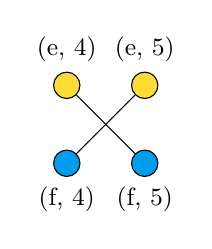
\begin{tikzpicture}[scale=0.33]
                    \node[draw, circle, fill=uofgsunshine, inner sep=0.5pt, font=\normalsize] (Me4) at (0, 3) {\phantom{0}};
                    \node[draw, circle, fill=uofgsunshine, inner sep=0.5pt, font=\normalsize] (Me5) at (3, 3) {\phantom{0}};
                    \node[draw, circle, fill=uofgcobalt, inner sep=0.5pt, font=\normalsize] (Mf4) at (0, 0) {\phantom{0}};
                    \node[draw, circle, fill=uofgcobalt, inner sep=0.5pt, font=\normalsize] (Mf5) at (3, 0) {\phantom{0}};

                    \node [above = 0 of Me4, font=\small] { \vphantom{0}(e, 4) };
                    \node [above = 0 of Me5, font=\small] { \vphantom{0}(e, 5) };
                    \node [below = 0 of Mf4, font=\small] { \vphantom{0}(f, 4) };
                    \node [below = 0 of Mf5, font=\small] { \vphantom{0}(f, 5) };

                    \draw (Me4) -- (Mf5);
                    \draw (Me5) -- (Mf4);
            \end{tikzpicture}
            &
            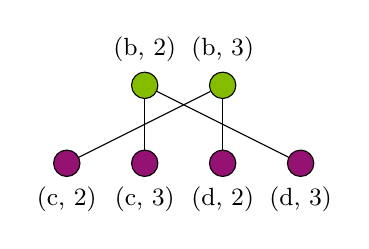
\begin{tikzpicture}[scale=0.33]
                    \node[draw, circle, fill=uofglawn, inner sep=0.5pt, font=\normalsize] (Mb2) at (3, 3) {\phantom{0}};
                    \node[draw, circle, fill=uofglawn, inner sep=0.5pt, font=\normalsize] (Mb3) at (6, 3) {\phantom{0}};
                    \node[draw, circle, fill=uofgthistle, inner sep=0.5pt, font=\normalsize] (Mc2) at (0, 0) {\phantom{0}};
                    \node[draw, circle, fill=uofgthistle, inner sep=0.5pt, font=\normalsize] (Mc3) at (3, 0) {\phantom{0}};
                    \node[draw, circle, fill=uofgthistle, inner sep=0.5pt, font=\normalsize] (Md2) at (6, 0) {\phantom{0}};
                    \node[draw, circle, fill=uofgthistle, inner sep=0.5pt, font=\normalsize] (Md3) at (9, 0) {\phantom{0}};

                    \node [above = 0 of Mb2, font=\small] { \vphantom{0}(b, 2) };
                    \node [above = 0 of Mb3, font=\small] { \vphantom{0}(b, 3) };
                    \node [below = 0 of Mc2, font=\small] { \vphantom{0}(c, 2) };
                    \node [below = 0 of Mc3, font=\small] { \vphantom{0}(c, 3) };
                    \node [below = 0 of Md2, font=\small] { \vphantom{0}(d, 2) };
                    \node [below = 0 of Md3, font=\small] { \vphantom{0}(d, 3) };

                    \draw (Mb2) -- (Mc3);
                    \draw (Mb2) -- (Md3);
                    \draw (Mb3) -- (Mc2);
                    \draw (Mb3) -- (Md2);
            \end{tikzpicture}
            \\[0.1cm]
            \stepcounter{stepcounter2}\roman{stepcounter2}) $\mathit{remaining} \setminus \mathit{branchable}$ &
            \stepcounter{stepcounter2}\roman{stepcounter2}) $\mathit{remaining} \cap \mathit{branchable}$
            \\
        };
    \end{tikzpicture}\\[0.3cm]\begin{tikzpicture}[scale=0.33]
        \matrix (m) [matrix of nodes] {
            \begin{tikzpicture}[scale=0.33]
                \node[draw, circle, fill=uofgsunshine, inner sep=0.5pt, font=\normalsize] (Me4) at (0, 0) {\phantom{0}};
                \node[draw, circle, fill=uofgsunshine, inner sep=0.5pt, font=\normalsize] (Me5) at (3, 0) {\phantom{0}};
                \node[draw, circle, fill=uofgcobalt, inner sep=0.5pt, font=\normalsize] (Mf4) at (6, 0) {\phantom{0}};
                \node[draw, circle, fill=uofgcobalt, inner sep=0.5pt, font=\normalsize] (Mf5) at (9, 0) {\phantom{0}};
                \node[draw, circle, fill=uofglawn, inner sep=0.5pt, font=\normalsize] (Mb2) at (12, 0) {\phantom{0}};
                \node[draw, circle, fill=uofglawn, inner sep=0.5pt, font=\normalsize] (Mb3) at (15, 0) {\phantom{0}};
                \node[draw, circle, fill=uofgthistle, inner sep=0.5pt, font=\normalsize] (Mc2) at (18, 0) {\phantom{0}};
                \node[draw, circle, fill=uofgthistle, inner sep=0.5pt, font=\normalsize] (Mc3) at (21, 0) {\phantom{0}};
                \node[draw, circle, fill=uofgthistle, inner sep=0.5pt, font=\normalsize] (Md2) at (24, 0) {\phantom{0}};
                \node[draw, circle, fill=uofgthistle, inner sep=0.5pt, font=\normalsize] (Md3) at (27, 0) {\phantom{0}};

                \node [above = 0 of Me4, font=\small, xshift=-0.5ex] { \vphantom{0}[[(e, 4), };
                \node [above = 0 of Me5, font=\small] { \vphantom{0}(e, 5)], };
                \node [above = 0 of Mf4, font=\small] { \vphantom{0}[(f, 4), };
                \node [above = 0 of Mf5, font=\small] { \vphantom{0}(f, 5)], };
                \node [above = 0 of Mb2, font=\small] { \vphantom{0}[(b, 2), };
                \node [above = 0 of Mb3, font=\small] { \vphantom{0}(b, 3)], };
                \node [above = 0 of Mc2, font=\small] { \vphantom{0}[(c, 2), };
                \node [above = 0 of Mc3, font=\small] { \vphantom{0}(c, 3), };
                \node [above = 0 of Md2, font=\small] { \vphantom{0}(d, 2), };
                \node [above = 0 of Md3, font=\small] { \vphantom{0}(d, 3)]]};
            \end{tikzpicture}
            \\[0.1cm]
            \stepcounter{stepcounter2}\roman{stepcounter2}) The resulting $\mathit{colourClasses}$ variable.
            \\
        };
    \end{tikzpicture}

    \caption{Solving a maximum common connected problem using an association graph. Suppose we
        have already mapped vertex $a$ to vertex $1$, giving the assignments on the right. Now we
        have two subgraphs to colour. We need two colours for $\mathit{remaining} \setminus
        \mathit{branchable}$, and we place these two colour classes first in the $\mathit{colourClasses}$
        variable. We can also colour $\mathit{remaining} \cap \mathit{branchable}$ using two
        colours, since we cannot simultaneously map $c$ to $2$ and $d$ to $3$, or vice-versa. Thus
        $\mathit{colourClasses}$ becomes a list of four colour classes, the first three containing
        two vertices each, and the last containing four vertices. This tells us that if we hope to
        extend the current common subgraph by another four vertices, we
        must pick one assignment from each of the four colour classes (which is not actually possible, so we
    see the bound here gives an overestimate). The algorithm thus guesses $d \mapsto 3$ as its next
assignment, and if that fails, $d \mapsto 2$, and so on; once $b \mapsto 3$ is reached, the bound
decreases by one, and if $f \mapsto 5$ were reached we would stop due to a lack of remaining
branchable vertices. }\label{figure:assocrestricted}
\end{figure}

It is not possible to determine connectedness from a raw association graph. However, we can take a
maximum clique algorithm and mimic the branching strategy if we have access to the underlying graphs
and can determine the ``meaning'' of the association graph vertices.

Most modern maximum clique algorithms for dense graphs use some variation of greedy graph colouring
as a bound---the underlying observation is that each vertex in a clique must be given a different
colour in a colouring, so if we can colour a subset of vertices using $k$ colours then a maximum
clique in this subset has at most $k$ vertices. However, the colouring is also used as a branching
heuristic: vertices are selected in reverse from their colour classes in turn, starting with the
last colour class created. Because of this coupling of branching and the bound (which is important
in practice because it mimics a ``smallest domain first'' branching heuristic if colour classes are
viewed as variables \cite{DBLP:conf/cp/McCreeshP14}), if we were to select only a subset of vertices for
branching at each stage inside a clique algorithm, we would lose completeness. Thus we must adapt
the bound to take into account restricted branching.

In \cref{algorithm:mccis} we present a clique-inspired algorithm which finds a maximum common
connected induced subgraph isomorphism via an
association graph. If the additional
branching restrictions are removed, the core of the algorithm is what Prosser
\cite{DBLP:journals/algorithms/Prosser12} calls the ``MCSa1'' variant of a series of algorithms due
to Tomita \textit{et al.}\
\cite{DBLP:conf/dmtcs/TomitaS03,DBLP:journals/jgo/TomitaK07,DBLP:conf/walcom/TomitaSHTW10}, using a
bitset encoding due to San Segundo \textit{et al.}\
\cite{DBLP:journals/cor/SegundoRJ11,DBLP:journals/ol/SegundoMRH13} (and we refer the reader to these
papers for implementation details on how to use bitsets and other data structures to implement the
colouring stage with very low constant factors).

We begin by building the association graph (\lineref{buildassoc}). The main part of the algorithm
then works by building up candidate cliques in the $\mathit{solution}$ variable, by recursive calls
to the $\mathit{search}$ procedure---starting from the empty set (\lineref{firstsearch}), each
recursive subcall adds one vertex to $\mathit{solution}$ (\lineref{addv}) in such a way that
$\mathit{solution}$ is always a clique which corresponds to a connected common subgraph. The
$\mathit{remaining}$ set contains the set of vertices which are adjacent to every vertex in
$\mathit{solution}$, and which have not yet been accepted or rejected (and so initially it contains
every vertex). The main loops in the $\FuncSty{search}$ procedure
(\twolinesref{outerloop}{innerloop}) have the effect of iterating over each vertex in this set in a
particular order---each vertex $v$ is selected in turn, and then a recursive call is made to
consider the effects of including $v$ in $\mathit{solution}$ (\lineref{recursesearch}), followed by
the next iteration where $v$ is instead rejected. When $v$ is accepted, we add it to the new
$\mathit{solution'}$ (\lineref{addvtosolution}), and create a new $\mathit{remaining'}$ containing
only the vertices in $\mathit{remaining}$ which are adjacent to $v$ (\lineref{filterremaining}).

The $\mathit{branchable}$ set contains the set of association graph vertices which correspond to
vertices adjacent to an already-accepted vertex in the first input graph---in constraint programming terms, it is the
set of assignments which could be made next which preserve connectedness. (Using only one of the two
input graphs is sufficient for correctness, and has the advantage that the $\FuncSty{connected}$
function may be implemented as a simple lookup into a precomputed array which maps each vertex in
the first input graph to a bitset.) At the top of search, this set is empty, and is not used (our
first vertex selection is special, and does not care about connectedness). At subsequent depths, we
may only accept vertices which are in this set, and if no such vertices remain then we return
immediately (\lineref{acceptbranchable}). When recursing, we extend $\mathit{branchable}$ with the
new vertices permitted by our acceptance of the branching $v$ (\lineref{addtobranchable}). Note that
we are assuming that inside the main loops, we encounter every vertex in $\mathit{remaining} \cap
\mathit{connected}$ before any vertex in $\mathit{remaining} \setminus \mathit{connected}$.

As we proceed, we keep track of the best solution we have found so far---this is stored in the
$\mathit{incumbent}$ variable (\twolinesref{incumbent}{newincumbent}). We use the incumbent,
together with a colour bound, to prune portions of the search space which cannot contain a better
solution. The colour bound operates as follows: at each entry to the $\FuncSty{search}$ procedure,
we produce a greedy colouring of the vertices in $\mathit{remaining}$ (\lineref{makecolours}). This
greedy colouring gives us a list of colour classes, each of which is a list of pairwise non-adjacent
vertices. The two loops (\twolinesref{outerloop}{innerloop}) then iterate over each colour class,
from last to first, and then over each vertex in that colour class, again from last to first.
(Rather than actually using a list of lists and removing items, this process should be implemented
using a pair of immutable flat arrays. This technique is described elsewhere
\cite{DBLP:conf/cp/McCreeshP14}, so we do not discuss it here.) Finally, if at any point the number
of remaining colour classes plus the number of vertices currently present in $\mathit{solution}$ is
not strictly greater than the size of the incumbent, then we may backtrack immediately
(\lineref{bound}).

Finally, we describe the colouring process. In conventional clique algorithms, a simple greedy
sequential colouring is used (possibly with the help of previous colourings to reduce the
computational cost \cite{DBLP:conf/lion/NikolaevBS15}, and possibly with shortcuts taken for certain
vertices \cite{DBLP:journals/cor/SegundoT14}, and possibly followed by a repair step to
improve the colouring \cite{DBLP:conf/walcom/TomitaSHTW10}, or stronger bounding rules based upon
MaxSAT inference \cite{DBLP:conf/ictai/LiFX13,DBLP:conf/lion/LiJX15,DBLP:journals/cor/SegundoNB15}).
Such colourings will not give us the required property that vertices in $\mathit{remaining} \cap
\mathit{connected}$ come last (so they are selected first by the reverse branching order). Thus we
produce two greedy sequential colourings, first considering the non-branching vertices in
$\mathit{remaining} \setminus \mathit{connected}$, followed by the branching vertices, and
concatenate them (\lineref{makecolours}). This produces a valid colouring, since we do not merge any
colour classes between the two stages, although it may use more colours than a single colouring
would\footnote{What if we did not guarantee that vertices in $\mathit{remaining} \cap
    \mathit{connected}$ came last, and just used a conventional colouring with the branching rule?
    Suppose we had four vertices in $\mathit{remaining}$, and produced a colouring $[[v_1, v_2],
    [v_3], [v_4]]$, and suppose that extending $\mathit{solution}$ with $\{ v_1, v_3, v_4 \}$ gives
an optimal solution. If $v_4$ was not $\mathit{connected}$ yet, we would not branch on that subtree,
and the bound could eliminate branching on $v_3$ and $v_1$, so we would miss the solution. Thus we
cannot simply add the branching rule without also adapting the combined bound / ordering heuristic.}.

Our $\FuncSty{colour}$ procedure is the same as the bit-parallel algorithm introduced by San Segundo
\textit{et al.}\ \cite{DBLP:journals/cor/SegundoRJ11}. While we have remaining vertices to colour
(\lineref{whileuncoloured}), we start a new colour class (\lineref{newcolourclass}), and then
repeatedly pick a legal vertex to add to that colour class (\lineref{addtocolourclass}).  The
selection of the next vertex to colour (\lineref{selectvtocolour}) may be performed efficiently in
hardware if the association graph is permuted to be in degree order at the top of search. Other
initial vertex orderings have been considered on general clique problems
\cite{DBLP:journals/algorithms/Prosser12,DBLP:conf/lion/SegundoLB14}; it is possible that special
properties of the association graph could be exploited in this step.


\subsection{Experimental comparison of CP with the Clique-based Approach}\label{mccs-eval}


\paragraph{Connected, Undirected, 33\% Labelled}

\paragraph{Connected, Undirected, Unlabelled}

?? My gut feeling is that if we have edge labels, the clique model wins, and if we don't, it's
likely to lose. So maybe I should run some experiments with vertex labels but not edge labels to
test this.

\paragraph{By family} ?? Break this down more by family, size, etc.

\paragraph{Does connected make instances easier or harder?} We could plot connected vs not connected
difficulties, and result sizes?

\begin{figure}[p]
    \centering
    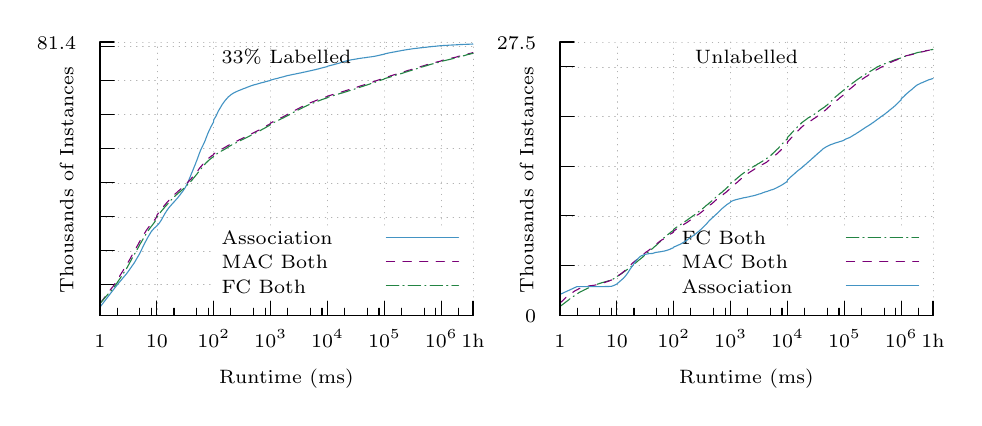
\begin{tikzpicture}[gnuplot]
%% generated with GNUPLOT 5.0p0 (Lua 5.2; terminal rev. 99, script rev. 100)
%% Wed 20 Apr 2016 10:28:40 AEST
\tikzset{every node/.append style={font={\scriptsize}}}
% \path (0.000,0.000) rectangle (11.684,4.826);
\gpcolor{color=gp lt color axes}
\gpsetlinetype{gp lt axes}
\gpsetdashtype{gp dt axes}
\gpsetlinewidth{0.50}
\draw[gp path] (0.552,1.374)--(1.981,1.374);
\gpcolor{color=gp lt color border}
\gpsetlinetype{gp lt border}
\gpsetdashtype{gp dt solid}
\gpsetlinewidth{1.00}
\draw[gp path] (0.552,1.374)--(0.732,1.374);
\gpcolor{color=gp lt color axes}
\gpsetlinetype{gp lt axes}
\gpsetdashtype{gp dt axes}
\gpsetlinewidth{0.50}
\draw[gp path] (0.552,1.805)--(1.981,1.805);
\gpcolor{color=gp lt color border}
\gpsetlinetype{gp lt border}
\gpsetdashtype{gp dt solid}
\gpsetlinewidth{1.00}
\draw[gp path] (0.552,1.805)--(0.732,1.805);
\gpcolor{color=gp lt color axes}
\gpsetlinetype{gp lt axes}
\gpsetdashtype{gp dt axes}
\gpsetlinewidth{0.50}
\draw[gp path] (0.552,2.237)--(5.289,2.237);
\gpcolor{color=gp lt color border}
\gpsetlinetype{gp lt border}
\gpsetdashtype{gp dt solid}
\gpsetlinewidth{1.00}
\draw[gp path] (0.552,2.237)--(0.732,2.237);
\gpcolor{color=gp lt color axes}
\gpsetlinetype{gp lt axes}
\gpsetdashtype{gp dt axes}
\gpsetlinewidth{0.50}
\draw[gp path] (0.552,2.669)--(5.289,2.669);
\gpcolor{color=gp lt color border}
\gpsetlinetype{gp lt border}
\gpsetdashtype{gp dt solid}
\gpsetlinewidth{1.00}
\draw[gp path] (0.552,2.669)--(0.732,2.669);
\gpcolor{color=gp lt color axes}
\gpsetlinetype{gp lt axes}
\gpsetdashtype{gp dt axes}
\gpsetlinewidth{0.50}
\draw[gp path] (0.552,3.101)--(5.289,3.101);
\gpcolor{color=gp lt color border}
\gpsetlinetype{gp lt border}
\gpsetdashtype{gp dt solid}
\gpsetlinewidth{1.00}
\draw[gp path] (0.552,3.101)--(0.732,3.101);
\gpcolor{color=gp lt color axes}
\gpsetlinetype{gp lt axes}
\gpsetdashtype{gp dt axes}
\gpsetlinewidth{0.50}
\draw[gp path] (0.552,3.533)--(5.289,3.533);
\gpcolor{color=gp lt color border}
\gpsetlinetype{gp lt border}
\gpsetdashtype{gp dt solid}
\gpsetlinewidth{1.00}
\draw[gp path] (0.552,3.533)--(0.732,3.533);
\gpcolor{color=gp lt color axes}
\gpsetlinetype{gp lt axes}
\gpsetdashtype{gp dt axes}
\gpsetlinewidth{0.50}
\draw[gp path] (0.552,3.965)--(5.289,3.965);
\gpcolor{color=gp lt color border}
\gpsetlinetype{gp lt border}
\gpsetdashtype{gp dt solid}
\gpsetlinewidth{1.00}
\draw[gp path] (0.552,3.965)--(0.732,3.965);
\gpcolor{color=gp lt color axes}
\gpsetlinetype{gp lt axes}
\gpsetdashtype{gp dt axes}
\gpsetlinewidth{0.50}
\draw[gp path] (0.552,4.397)--(5.289,4.397);
\gpcolor{color=gp lt color border}
\gpsetlinetype{gp lt border}
\gpsetdashtype{gp dt solid}
\gpsetlinewidth{1.00}
\draw[gp path] (0.552,4.397)--(0.732,4.397);
\gpcolor{color=gp lt color axes}
\gpsetlinetype{gp lt axes}
\gpsetdashtype{gp dt axes}
\gpsetlinewidth{0.50}
\draw[gp path] (0.552,4.457)--(5.289,4.457);
\gpcolor{color=gp lt color border}
\gpsetlinetype{gp lt border}
\gpsetdashtype{gp dt solid}
\gpsetlinewidth{1.00}
\draw[gp path] (0.552,4.457)--(0.732,4.457);
\node[gp node right] at (0.368,4.457) {81.4};
\gpcolor{color=gp lt color axes}
\gpsetlinetype{gp lt axes}
\gpsetdashtype{gp dt axes}
\gpsetlinewidth{0.50}
\draw[gp path] (0.552,1.374)--(1.981,1.374);
\gpcolor{color=gp lt color border}
\gpsetlinetype{gp lt border}
\gpsetdashtype{gp dt solid}
\gpsetlinewidth{1.00}
\draw[gp path] (0.552,1.374)--(0.732,1.374);
\gpcolor{color=gp lt color axes}
\gpsetlinetype{gp lt axes}
\gpsetdashtype{gp dt axes}
\gpsetlinewidth{0.50}
\draw[gp path] (0.552,1.805)--(1.981,1.805);
\gpcolor{color=gp lt color border}
\gpsetlinetype{gp lt border}
\gpsetdashtype{gp dt solid}
\gpsetlinewidth{1.00}
\draw[gp path] (0.552,1.805)--(0.732,1.805);
\gpcolor{color=gp lt color axes}
\gpsetlinetype{gp lt axes}
\gpsetdashtype{gp dt axes}
\gpsetlinewidth{0.50}
\draw[gp path] (0.552,2.237)--(5.289,2.237);
\gpcolor{color=gp lt color border}
\gpsetlinetype{gp lt border}
\gpsetdashtype{gp dt solid}
\gpsetlinewidth{1.00}
\draw[gp path] (0.552,2.237)--(0.732,2.237);
\gpcolor{color=gp lt color axes}
\gpsetlinetype{gp lt axes}
\gpsetdashtype{gp dt axes}
\gpsetlinewidth{0.50}
\draw[gp path] (0.552,2.669)--(5.289,2.669);
\gpcolor{color=gp lt color border}
\gpsetlinetype{gp lt border}
\gpsetdashtype{gp dt solid}
\gpsetlinewidth{1.00}
\draw[gp path] (0.552,2.669)--(0.732,2.669);
\gpcolor{color=gp lt color axes}
\gpsetlinetype{gp lt axes}
\gpsetdashtype{gp dt axes}
\gpsetlinewidth{0.50}
\draw[gp path] (0.552,3.101)--(5.289,3.101);
\gpcolor{color=gp lt color border}
\gpsetlinetype{gp lt border}
\gpsetdashtype{gp dt solid}
\gpsetlinewidth{1.00}
\draw[gp path] (0.552,3.101)--(0.732,3.101);
\gpcolor{color=gp lt color axes}
\gpsetlinetype{gp lt axes}
\gpsetdashtype{gp dt axes}
\gpsetlinewidth{0.50}
\draw[gp path] (0.552,3.533)--(5.289,3.533);
\gpcolor{color=gp lt color border}
\gpsetlinetype{gp lt border}
\gpsetdashtype{gp dt solid}
\gpsetlinewidth{1.00}
\draw[gp path] (0.552,3.533)--(0.732,3.533);
\gpcolor{color=gp lt color axes}
\gpsetlinetype{gp lt axes}
\gpsetdashtype{gp dt axes}
\gpsetlinewidth{0.50}
\draw[gp path] (0.552,3.965)--(5.289,3.965);
\gpcolor{color=gp lt color border}
\gpsetlinetype{gp lt border}
\gpsetdashtype{gp dt solid}
\gpsetlinewidth{1.00}
\draw[gp path] (0.552,3.965)--(0.732,3.965);
\gpcolor{color=gp lt color axes}
\gpsetlinetype{gp lt axes}
\gpsetdashtype{gp dt axes}
\gpsetlinewidth{0.50}
\draw[gp path] (0.552,4.397)--(5.289,4.397);
\gpcolor{color=gp lt color border}
\gpsetlinetype{gp lt border}
\gpsetdashtype{gp dt solid}
\gpsetlinewidth{1.00}
\draw[gp path] (0.552,4.397)--(0.732,4.397);
\gpcolor{color=gp lt color axes}
\gpsetlinetype{gp lt axes}
\gpsetdashtype{gp dt axes}
\gpsetlinewidth{0.50}
\draw[gp path] (0.552,0.985)--(0.552,4.457);
\gpcolor{color=gp lt color border}
\gpsetlinetype{gp lt border}
\gpsetdashtype{gp dt solid}
\gpsetlinewidth{1.00}
\draw[gp path] (0.552,0.985)--(0.552,1.165);
\node[gp node center] at (0.552,0.677) {1};
\gpcolor{color=gp lt color axes}
\gpsetlinetype{gp lt axes}
\gpsetdashtype{gp dt axes}
\gpsetlinewidth{0.50}
\draw[gp path] (1.275,0.985)--(1.275,4.457);
\gpcolor{color=gp lt color border}
\gpsetlinetype{gp lt border}
\gpsetdashtype{gp dt solid}
\gpsetlinewidth{1.00}
\draw[gp path] (1.275,0.985)--(1.275,1.165);
\node[gp node center] at (1.275,0.677) {10};
\gpcolor{color=gp lt color axes}
\gpsetlinetype{gp lt axes}
\gpsetdashtype{gp dt axes}
\gpsetlinewidth{0.50}
\draw[gp path] (5.289,0.985)--(5.289,4.457);
\gpcolor{color=gp lt color border}
\gpsetlinetype{gp lt border}
\gpsetdashtype{gp dt solid}
\gpsetlinewidth{1.00}
\draw[gp path] (5.289,0.985)--(5.289,1.165);
\node[gp node center] at (5.289,0.677) {1h};
\gpcolor{color=gp lt color axes}
\gpsetlinetype{gp lt axes}
\gpsetdashtype{gp dt axes}
\gpsetlinewidth{0.50}
\draw[gp path] (0.552,0.985)--(0.552,4.457);
\gpcolor{color=gp lt color border}
\gpsetlinetype{gp lt border}
\gpsetdashtype{gp dt solid}
\gpsetlinewidth{1.00}
\draw[gp path] (0.552,0.985)--(0.552,1.165);
\draw[gp path] (0.769,0.985)--(0.769,1.075);
\draw[gp path] (1.057,0.985)--(1.057,1.075);
\draw[gp path] (1.204,0.985)--(1.204,1.075);
\gpcolor{color=gp lt color axes}
\gpsetlinetype{gp lt axes}
\gpsetdashtype{gp dt axes}
\gpsetlinewidth{0.50}
\draw[gp path] (1.275,0.985)--(1.275,4.457);
\gpcolor{color=gp lt color border}
\gpsetlinetype{gp lt border}
\gpsetdashtype{gp dt solid}
\gpsetlinewidth{1.00}
\draw[gp path] (1.275,0.985)--(1.275,1.165);
\draw[gp path] (1.492,0.985)--(1.492,1.075);
\draw[gp path] (1.780,0.985)--(1.780,1.075);
\draw[gp path] (1.927,0.985)--(1.927,1.075);
\gpcolor{color=gp lt color axes}
\gpsetlinetype{gp lt axes}
\gpsetdashtype{gp dt axes}
\gpsetlinewidth{0.50}
\draw[gp path] (1.997,0.985)--(1.997,1.207);
\draw[gp path] (1.997,2.131)--(1.997,4.457);
\gpcolor{color=gp lt color border}
\gpsetlinetype{gp lt border}
\gpsetdashtype{gp dt solid}
\gpsetlinewidth{1.00}
\draw[gp path] (1.997,0.985)--(1.997,1.165);
\node[gp node center] at (1.997,0.677) {$10^{2}$};
\draw[gp path] (2.215,0.985)--(2.215,1.075);
\draw[gp path] (2.502,0.985)--(2.502,1.075);
\draw[gp path] (2.650,0.985)--(2.650,1.075);
\gpcolor{color=gp lt color axes}
\gpsetlinetype{gp lt axes}
\gpsetdashtype{gp dt axes}
\gpsetlinewidth{0.50}
\draw[gp path] (2.720,0.985)--(2.720,1.207);
\draw[gp path] (2.720,2.131)--(2.720,4.457);
\gpcolor{color=gp lt color border}
\gpsetlinetype{gp lt border}
\gpsetdashtype{gp dt solid}
\gpsetlinewidth{1.00}
\draw[gp path] (2.720,0.985)--(2.720,1.165);
\node[gp node center] at (2.720,0.677) {$10^{3}$};
\draw[gp path] (2.937,0.985)--(2.937,1.075);
\draw[gp path] (3.225,0.985)--(3.225,1.075);
\draw[gp path] (3.372,0.985)--(3.372,1.075);
\gpcolor{color=gp lt color axes}
\gpsetlinetype{gp lt axes}
\gpsetdashtype{gp dt axes}
\gpsetlinewidth{0.50}
\draw[gp path] (3.442,0.985)--(3.442,1.207);
\draw[gp path] (3.442,2.131)--(3.442,4.457);
\gpcolor{color=gp lt color border}
\gpsetlinetype{gp lt border}
\gpsetdashtype{gp dt solid}
\gpsetlinewidth{1.00}
\draw[gp path] (3.442,0.985)--(3.442,1.165);
\node[gp node center] at (3.442,0.677) {$10^{4}$};
\draw[gp path] (3.660,0.985)--(3.660,1.075);
\draw[gp path] (3.947,0.985)--(3.947,1.075);
\draw[gp path] (4.095,0.985)--(4.095,1.075);
\gpcolor{color=gp lt color axes}
\gpsetlinetype{gp lt axes}
\gpsetdashtype{gp dt axes}
\gpsetlinewidth{0.50}
\draw[gp path] (4.165,0.985)--(4.165,1.207);
\draw[gp path] (4.165,2.131)--(4.165,4.457);
\gpcolor{color=gp lt color border}
\gpsetlinetype{gp lt border}
\gpsetdashtype{gp dt solid}
\gpsetlinewidth{1.00}
\draw[gp path] (4.165,0.985)--(4.165,1.165);
\node[gp node center] at (4.165,0.677) {$10^{5}$};
\draw[gp path] (4.382,0.985)--(4.382,1.075);
\draw[gp path] (4.670,0.985)--(4.670,1.075);
\draw[gp path] (4.817,0.985)--(4.817,1.075);
\gpcolor{color=gp lt color axes}
\gpsetlinetype{gp lt axes}
\gpsetdashtype{gp dt axes}
\gpsetlinewidth{0.50}
\draw[gp path] (4.887,0.985)--(4.887,1.207);
\draw[gp path] (4.887,2.131)--(4.887,4.457);
\gpcolor{color=gp lt color border}
\gpsetlinetype{gp lt border}
\gpsetdashtype{gp dt solid}
\gpsetlinewidth{1.00}
\draw[gp path] (4.887,0.985)--(4.887,1.165);
\node[gp node center] at (4.887,0.677) {$10^{6}$};
\draw[gp path] (5.105,0.985)--(5.105,1.075);
\draw[gp path] (0.552,4.457)--(0.552,0.985)--(5.289,0.985);
\node[gp node center,rotate=-270] at (0.140,2.721) {Thousands of Instances};
\node[gp node center] at (2.920,0.215) {Runtime (ms)};
\node[gp node left] at (1.981,1.977) {Association};
\gpcolor{rgb color={0.263,0.576,0.765}}
\draw[gp path] (4.189,1.977)--(5.105,1.977);
\draw[gp path] (0.552,1.090)--(0.769,1.371)--(0.897,1.523)--(0.987,1.651)--(1.057,1.771)%
  --(1.114,1.890)--(1.163,1.982)--(1.204,2.050)--(1.241,2.092)--(1.275,2.122)--(1.304,2.155)%
  --(1.332,2.197)--(1.357,2.242)--(1.380,2.283)--(1.402,2.317)--(1.422,2.345)--(1.441,2.368)%
  --(1.459,2.389)--(1.476,2.408)--(1.492,2.425)--(1.507,2.441)--(1.522,2.459)--(1.536,2.473)%
  --(1.549,2.491)--(1.562,2.506)--(1.574,2.522)--(1.586,2.539)--(1.598,2.554)--(1.609,2.569)%
  --(1.619,2.584)--(1.630,2.599)--(1.639,2.616)--(1.649,2.634)--(1.659,2.653)--(1.668,2.671)%
  --(1.676,2.692)--(1.685,2.714)--(1.693,2.733)--(1.702,2.754)--(1.710,2.775)--(1.717,2.794)%
  --(1.725,2.810)--(1.732,2.828)--(1.739,2.846)--(1.746,2.863)--(1.753,2.880)--(1.760,2.897)%
  --(1.767,2.915)--(1.773,2.932)--(1.780,2.948)--(1.786,2.964)--(1.792,2.981)--(1.798,2.998)%
  --(1.804,3.013)--(1.809,3.029)--(1.815,3.045)--(1.821,3.058)--(1.826,3.072)--(1.831,3.086)%
  --(1.837,3.098)--(1.842,3.108)--(1.847,3.119)--(1.852,3.128)--(1.857,3.138)--(1.862,3.149)%
  --(1.867,3.160)--(1.871,3.170)--(1.876,3.179)--(1.881,3.189)--(1.885,3.200)--(1.890,3.210)%
  --(1.894,3.222)--(1.898,3.235)--(1.903,3.246)--(1.907,3.256)--(1.911,3.267)--(1.915,3.277)%
  --(1.919,3.288)--(1.923,3.297)--(1.927,3.305)--(1.931,3.315)--(1.935,3.324)--(1.939,3.332)%
  --(1.942,3.340)--(1.946,3.347)--(1.950,3.356)--(1.953,3.363)--(1.957,3.370)--(1.960,3.378)%
  --(1.964,3.385)--(1.967,3.390)--(1.971,3.397)--(1.974,3.403)--(1.978,3.410)--(1.981,3.416)%
  --(1.984,3.422)--(1.987,3.427)--(1.991,3.433)--(1.994,3.439)--(1.997,3.470)--(2.027,3.517)%
  --(2.054,3.578)--(2.079,3.619)--(2.103,3.661)--(2.124,3.690)--(2.145,3.718)--(2.164,3.739)%
  --(2.181,3.759)--(2.198,3.772)--(2.215,3.787)--(2.230,3.796)--(2.244,3.806)--(2.258,3.813)%
  --(2.272,3.821)--(2.285,3.827)--(2.297,3.832)--(2.309,3.837)--(2.320,3.842)--(2.331,3.846)%
  --(2.342,3.851)--(2.352,3.854)--(2.362,3.859)--(2.372,3.863)--(2.381,3.867)--(2.390,3.869)%
  --(2.399,3.873)--(2.408,3.876)--(2.416,3.880)--(2.424,3.884)--(2.432,3.886)--(2.440,3.888)%
  --(2.447,3.891)--(2.455,3.894)--(2.462,3.897)--(2.469,3.899)--(2.476,3.903)--(2.483,3.904)%
  --(2.489,3.907)--(2.496,3.908)--(2.502,3.911)--(2.508,3.912)--(2.514,3.914)--(2.520,3.916)%
  --(2.526,3.917)--(2.532,3.918)--(2.538,3.920)--(2.543,3.922)--(2.549,3.923)--(2.554,3.924)%
  --(2.559,3.926)--(2.564,3.928)--(2.570,3.930)--(2.575,3.931)--(2.579,3.932)--(2.584,3.934)%
  --(2.589,3.936)--(2.594,3.937)--(2.599,3.938)--(2.603,3.939)--(2.608,3.940)--(2.612,3.941)%
  --(2.616,3.942)--(2.621,3.943)--(2.625,3.944)--(2.629,3.945)--(2.633,3.946)--(2.638,3.948)%
  --(2.642,3.949)--(2.646,3.950)--(2.650,3.951)--(2.653,3.952)--(2.657,3.953)--(2.661,3.954)%
  --(2.665,3.955)--(2.669,3.956)--(2.672,3.957)--(2.676,3.958)--(2.679,3.959)--(2.683,3.960)%
  --(2.686,3.962)--(2.690,3.962)--(2.693,3.963)--(2.697,3.964)--(2.700,3.965)--(2.703,3.965)%
  --(2.707,3.966)--(2.710,3.967)--(2.713,3.968)--(2.716,3.969)--(2.720,3.974)--(2.749,3.981)%
  --(2.777,3.989)--(2.802,3.994)--(2.825,4.001)--(2.847,4.007)--(2.867,4.012)--(2.886,4.016)%
  --(2.904,4.022)--(2.921,4.027)--(2.937,4.031)--(2.952,4.034)--(2.967,4.037)--(2.981,4.040)%
  --(2.994,4.043)--(3.007,4.045)--(3.019,4.048)--(3.031,4.050)--(3.043,4.053)--(3.054,4.055)%
  --(3.064,4.057)--(3.075,4.059)--(3.085,4.062)--(3.094,4.063)--(3.104,4.065)--(3.113,4.067)%
  --(3.121,4.069)--(3.130,4.071)--(3.138,4.073)--(3.147,4.074)--(3.155,4.076)--(3.162,4.078)%
  --(3.170,4.079)--(3.177,4.081)--(3.184,4.083)--(3.191,4.085)--(3.198,4.086)--(3.205,4.088)%
  --(3.212,4.089)--(3.218,4.090)--(3.225,4.092)--(3.231,4.093)--(3.237,4.094)--(3.243,4.096)%
  --(3.249,4.097)--(3.254,4.098)--(3.260,4.100)--(3.266,4.101)--(3.271,4.102)--(3.276,4.104)%
  --(3.282,4.104)--(3.287,4.106)--(3.292,4.107)--(3.297,4.108)--(3.302,4.110)--(3.307,4.111)%
  --(3.312,4.112)--(3.316,4.113)--(3.321,4.114)--(3.326,4.115)--(3.330,4.116)--(3.335,4.118)%
  --(3.339,4.119)--(3.343,4.121)--(3.348,4.122)--(3.352,4.123)--(3.356,4.124)--(3.360,4.125)%
  --(3.364,4.126)--(3.368,4.127)--(3.372,4.128)--(3.376,4.129)--(3.380,4.130)--(3.384,4.131)%
  --(3.387,4.132)--(3.391,4.133)--(3.395,4.134)--(3.398,4.134)--(3.402,4.135)--(3.405,4.136)%
  --(3.409,4.137)--(3.412,4.138)--(3.416,4.138)--(3.419,4.140)--(3.423,4.141)--(3.426,4.141)%
  --(3.429,4.142)--(3.432,4.143)--(3.436,4.143)--(3.439,4.144)--(3.442,4.149)--(3.472,4.157)%
  --(3.499,4.164)--(3.524,4.170)--(3.548,4.177)--(3.569,4.183)--(3.590,4.188)--(3.609,4.195)%
  --(3.626,4.201)--(3.643,4.206)--(3.660,4.211)--(3.675,4.215)--(3.689,4.219)--(3.703,4.223)%
  --(3.717,4.225)--(3.730,4.228)--(3.742,4.230)--(3.754,4.233)--(3.765,4.234)--(3.776,4.236)%
  --(3.787,4.238)--(3.797,4.239)--(3.807,4.241)--(3.817,4.243)--(3.826,4.245)--(3.835,4.246)%
  --(3.844,4.248)--(3.853,4.249)--(3.861,4.250)--(3.869,4.251)--(3.877,4.252)--(3.885,4.254)%
  --(3.892,4.255)--(3.900,4.255)--(3.907,4.256)--(3.914,4.257)--(3.921,4.258)--(3.928,4.259)%
  --(3.934,4.260)--(3.941,4.261)--(3.947,4.262)--(3.953,4.263)--(3.959,4.264)--(3.965,4.264)%
  --(3.971,4.265)--(3.977,4.266)--(3.983,4.267)--(3.988,4.268)--(3.994,4.268)--(3.999,4.269)%
  --(4.004,4.270)--(4.009,4.271)--(4.015,4.271)--(4.020,4.272)--(4.025,4.273)--(4.029,4.274)%
  --(4.034,4.275)--(4.039,4.275)--(4.044,4.276)--(4.048,4.277)--(4.053,4.278)--(4.057,4.279)%
  --(4.061,4.280)--(4.066,4.281)--(4.070,4.282)--(4.074,4.283)--(4.078,4.284)--(4.083,4.285)%
  --(4.087,4.286)--(4.091,4.286)--(4.095,4.287)--(4.098,4.288)--(4.102,4.289)--(4.106,4.290)%
  --(4.110,4.291)--(4.114,4.292)--(4.117,4.292)--(4.121,4.293)--(4.124,4.294)--(4.128,4.295)%
  --(4.131,4.295)--(4.135,4.296)--(4.138,4.297)--(4.142,4.298)--(4.145,4.298)--(4.148,4.299)%
  --(4.152,4.300)--(4.155,4.301)--(4.158,4.302)--(4.161,4.302)--(4.165,4.305)--(4.194,4.312)%
  --(4.222,4.318)--(4.247,4.323)--(4.270,4.327)--(4.292,4.331)--(4.312,4.335)--(4.331,4.339)%
  --(4.349,4.342)--(4.366,4.345)--(4.382,4.348)--(4.397,4.351)--(4.412,4.353)--(4.426,4.356)%
  --(4.439,4.358)--(4.452,4.360)--(4.464,4.362)--(4.476,4.364)--(4.488,4.365)--(4.499,4.367)%
  --(4.509,4.369)--(4.520,4.370)--(4.530,4.372)--(4.539,4.373)--(4.549,4.374)--(4.558,4.375)%
  --(4.566,4.376)--(4.575,4.377)--(4.583,4.378)--(4.592,4.379)--(4.600,4.380)--(4.607,4.381)%
  --(4.615,4.382)--(4.622,4.383)--(4.629,4.384)--(4.637,4.384)--(4.643,4.385)--(4.650,4.386)%
  --(4.657,4.386)--(4.663,4.387)--(4.670,4.388)--(4.676,4.388)--(4.682,4.389)--(4.688,4.390)%
  --(4.694,4.390)--(4.699,4.391)--(4.705,4.392)--(4.711,4.392)--(4.716,4.393)--(4.722,4.394)%
  --(4.727,4.395)--(4.732,4.395)--(4.737,4.396)--(4.742,4.396)--(4.747,4.397)--(4.752,4.397)%
  --(4.757,4.398)--(4.761,4.398)--(4.766,4.399)--(4.771,4.400)--(4.775,4.400)--(4.780,4.400)%
  --(4.784,4.401)--(4.788,4.401)--(4.793,4.402)--(4.797,4.402)--(4.801,4.402)--(4.805,4.402)%
  --(4.809,4.403)--(4.813,4.403)--(4.817,4.403)--(4.821,4.404)--(4.825,4.404)--(4.829,4.405)%
  --(4.832,4.405)--(4.836,4.406)--(4.840,4.406)--(4.843,4.406)--(4.847,4.406)--(4.850,4.407)%
  --(4.854,4.407)--(4.857,4.408)--(4.861,4.408)--(4.864,4.408)--(4.868,4.409)--(4.871,4.409)%
  --(4.874,4.409)--(4.878,4.409)--(4.881,4.409)--(4.884,4.410)--(4.887,4.411)--(4.917,4.412)%
  --(4.944,4.414)--(4.969,4.415)--(4.993,4.417)--(5.014,4.418)--(5.035,4.419)--(5.054,4.420)%
  --(5.072,4.421)--(5.088,4.422)--(5.105,4.423)--(5.120,4.424)--(5.134,4.425)--(5.148,4.425)%
  --(5.162,4.426)--(5.175,4.426)--(5.187,4.427)--(5.199,4.427)--(5.210,4.428)--(5.221,4.428)%
  --(5.232,4.428)--(5.242,4.429)--(5.252,4.429)--(5.262,4.430)--(5.271,4.430)--(5.280,4.431)%
  --(5.289,4.431);
\gpcolor{color=gp lt color border}
\node[gp node left] at (1.981,1.669) {MAC Both};
\gpcolor{rgb color={0.478,0.004,0.467}}
\gpsetdashtype{gp dt 2}
\draw[gp path] (4.189,1.669)--(5.105,1.669);
\draw[gp path] (0.552,1.139)--(0.582,1.173)--(0.609,1.211)--(0.634,1.246)--(0.658,1.277)%
  --(0.679,1.303)--(0.699,1.329)--(0.719,1.353)--(0.736,1.378)--(0.753,1.404)--(0.769,1.429)%
  --(0.785,1.455)--(0.799,1.478)--(0.813,1.502)--(0.827,1.524)--(0.840,1.544)--(0.852,1.565)%
  --(0.864,1.582)--(0.875,1.600)--(0.886,1.617)--(0.897,1.635)--(0.907,1.654)--(0.917,1.672)%
  --(0.927,1.689)--(0.936,1.706)--(0.945,1.723)--(0.954,1.739)--(0.963,1.755)--(0.971,1.770)%
  --(0.979,1.784)--(0.987,1.797)--(0.995,1.809)--(1.002,1.824)--(1.010,1.838)--(1.017,1.852)%
  --(1.024,1.864)--(1.031,1.876)--(1.038,1.888)--(1.044,1.902)--(1.051,1.913)--(1.057,1.924)%
  --(1.063,1.935)--(1.069,1.946)--(1.075,1.956)--(1.081,1.967)--(1.087,1.978)--(1.093,1.988)%
  --(1.098,1.998)--(1.104,2.006)--(1.109,2.015)--(1.114,2.023)--(1.119,2.030)--(1.125,2.038)%
  --(1.130,2.046)--(1.134,2.053)--(1.139,2.062)--(1.144,2.069)--(1.149,2.076)--(1.153,2.083)%
  --(1.158,2.089)--(1.163,2.095)--(1.167,2.101)--(1.171,2.106)--(1.176,2.112)--(1.180,2.117)%
  --(1.184,2.122)--(1.188,2.128)--(1.192,2.133)--(1.197,2.138)--(1.201,2.142)--(1.204,2.148)%
  --(1.208,2.152)--(1.212,2.157)--(1.216,2.162)--(1.220,2.166)--(1.224,2.170)--(1.227,2.175)%
  --(1.231,2.179)--(1.234,2.183)--(1.238,2.188)--(1.241,2.192)--(1.245,2.196)--(1.248,2.201)%
  --(1.252,2.205)--(1.255,2.210)--(1.258,2.214)--(1.262,2.219)--(1.265,2.224)--(1.268,2.228)%
  --(1.271,2.233)--(1.275,2.256)--(1.304,2.297)--(1.332,2.333)--(1.357,2.364)--(1.380,2.392)%
  --(1.402,2.418)--(1.422,2.440)--(1.441,2.462)--(1.459,2.481)--(1.476,2.498)--(1.492,2.514)%
  --(1.507,2.528)--(1.522,2.540)--(1.536,2.553)--(1.549,2.565)--(1.562,2.576)--(1.574,2.587)%
  --(1.586,2.597)--(1.598,2.608)--(1.609,2.619)--(1.619,2.629)--(1.630,2.639)--(1.639,2.648)%
  --(1.649,2.658)--(1.659,2.667)--(1.668,2.676)--(1.676,2.685)--(1.685,2.694)--(1.693,2.703)%
  --(1.702,2.710)--(1.710,2.719)--(1.717,2.729)--(1.725,2.738)--(1.732,2.746)--(1.739,2.755)%
  --(1.746,2.762)--(1.753,2.770)--(1.760,2.778)--(1.767,2.787)--(1.773,2.794)--(1.780,2.803)%
  --(1.786,2.811)--(1.792,2.819)--(1.798,2.828)--(1.804,2.836)--(1.809,2.845)--(1.815,2.852)%
  --(1.821,2.859)--(1.826,2.865)--(1.831,2.872)--(1.837,2.877)--(1.842,2.884)--(1.847,2.890)%
  --(1.852,2.896)--(1.857,2.902)--(1.862,2.908)--(1.867,2.915)--(1.871,2.920)--(1.876,2.926)%
  --(1.881,2.931)--(1.885,2.936)--(1.890,2.941)--(1.894,2.946)--(1.898,2.950)--(1.903,2.954)%
  --(1.907,2.959)--(1.911,2.962)--(1.915,2.966)--(1.919,2.969)--(1.923,2.974)--(1.927,2.977)%
  --(1.931,2.980)--(1.935,2.983)--(1.939,2.986)--(1.942,2.989)--(1.946,2.992)--(1.950,2.995)%
  --(1.953,2.997)--(1.957,3.000)--(1.960,3.004)--(1.964,3.006)--(1.967,3.008)--(1.971,3.011)%
  --(1.974,3.012)--(1.978,3.015)--(1.981,3.017)--(1.984,3.019)--(1.987,3.021)--(1.991,3.023)%
  --(1.994,3.025)--(1.997,3.036)--(2.027,3.055)--(2.054,3.071)--(2.079,3.085)--(2.103,3.098)%
  --(2.124,3.110)--(2.145,3.122)--(2.164,3.133)--(2.181,3.143)--(2.198,3.152)--(2.215,3.161)%
  --(2.230,3.169)--(2.244,3.177)--(2.258,3.184)--(2.272,3.191)--(2.285,3.197)--(2.297,3.202)%
  --(2.309,3.207)--(2.320,3.214)--(2.331,3.219)--(2.342,3.224)--(2.352,3.229)--(2.362,3.233)%
  --(2.372,3.238)--(2.381,3.243)--(2.390,3.247)--(2.399,3.252)--(2.408,3.257)--(2.416,3.260)%
  --(2.424,3.264)--(2.432,3.269)--(2.440,3.272)--(2.447,3.275)--(2.455,3.279)--(2.462,3.284)%
  --(2.469,3.287)--(2.476,3.290)--(2.483,3.294)--(2.489,3.297)--(2.496,3.300)--(2.502,3.303)%
  --(2.508,3.306)--(2.514,3.310)--(2.520,3.313)--(2.526,3.316)--(2.532,3.319)--(2.538,3.322)%
  --(2.543,3.325)--(2.549,3.328)--(2.554,3.330)--(2.559,3.332)--(2.564,3.335)--(2.570,3.337)%
  --(2.575,3.340)--(2.579,3.342)--(2.584,3.345)--(2.589,3.347)--(2.594,3.350)--(2.599,3.352)%
  --(2.603,3.354)--(2.608,3.357)--(2.612,3.359)--(2.616,3.361)--(2.621,3.364)--(2.625,3.366)%
  --(2.629,3.368)--(2.633,3.371)--(2.638,3.373)--(2.642,3.376)--(2.646,3.378)--(2.650,3.381)%
  --(2.653,3.383)--(2.657,3.385)--(2.661,3.387)--(2.665,3.389)--(2.669,3.392)--(2.672,3.395)%
  --(2.676,3.396)--(2.679,3.398)--(2.683,3.400)--(2.686,3.403)--(2.690,3.405)--(2.693,3.406)%
  --(2.697,3.408)--(2.700,3.410)--(2.703,3.412)--(2.707,3.413)--(2.710,3.415)--(2.713,3.417)%
  --(2.716,3.419)--(2.720,3.428)--(2.749,3.444)--(2.777,3.458)--(2.802,3.471)--(2.825,3.481)%
  --(2.847,3.493)--(2.867,3.501)--(2.886,3.511)--(2.904,3.521)--(2.921,3.531)--(2.937,3.539)%
  --(2.952,3.547)--(2.967,3.555)--(2.981,3.562)--(2.994,3.571)--(3.007,3.579)--(3.019,3.584)%
  --(3.031,3.590)--(3.043,3.596)--(3.054,3.602)--(3.064,3.608)--(3.075,3.613)--(3.085,3.618)%
  --(3.094,3.624)--(3.104,3.629)--(3.113,3.633)--(3.121,3.638)--(3.130,3.641)--(3.138,3.645)%
  --(3.147,3.649)--(3.155,3.654)--(3.162,3.657)--(3.170,3.662)--(3.177,3.665)--(3.184,3.669)%
  --(3.191,3.672)--(3.198,3.675)--(3.205,3.677)--(3.212,3.680)--(3.218,3.683)--(3.225,3.686)%
  --(3.231,3.688)--(3.237,3.690)--(3.243,3.693)--(3.249,3.695)--(3.254,3.697)--(3.260,3.699)%
  --(3.266,3.702)--(3.271,3.703)--(3.276,3.706)--(3.282,3.708)--(3.287,3.710)--(3.292,3.712)%
  --(3.297,3.714)--(3.302,3.716)--(3.307,3.718)--(3.312,3.720)--(3.316,3.722)--(3.321,3.723)%
  --(3.326,3.725)--(3.330,3.727)--(3.335,3.728)--(3.339,3.730)--(3.343,3.731)--(3.348,3.733)%
  --(3.352,3.734)--(3.356,3.736)--(3.360,3.737)--(3.364,3.739)--(3.368,3.741)--(3.372,3.742)%
  --(3.376,3.744)--(3.380,3.745)--(3.384,3.747)--(3.387,3.748)--(3.391,3.749)--(3.395,3.750)%
  --(3.398,3.751)--(3.402,3.753)--(3.405,3.754)--(3.409,3.755)--(3.412,3.756)--(3.416,3.757)%
  --(3.419,3.758)--(3.423,3.759)--(3.426,3.760)--(3.429,3.761)--(3.432,3.762)--(3.436,3.763)%
  --(3.439,3.764)--(3.442,3.770)--(3.472,3.778)--(3.499,3.787)--(3.524,3.794)--(3.548,3.801)%
  --(3.569,3.808)--(3.590,3.814)--(3.609,3.819)--(3.626,3.824)--(3.643,3.829)--(3.660,3.834)%
  --(3.675,3.840)--(3.689,3.843)--(3.703,3.848)--(3.717,3.852)--(3.730,3.856)--(3.742,3.859)%
  --(3.754,3.863)--(3.765,3.867)--(3.776,3.870)--(3.787,3.874)--(3.797,3.877)--(3.807,3.880)%
  --(3.817,3.884)--(3.826,3.887)--(3.835,3.890)--(3.844,3.893)--(3.853,3.896)--(3.861,3.899)%
  --(3.869,3.901)--(3.877,3.904)--(3.885,3.906)--(3.892,3.908)--(3.900,3.911)--(3.907,3.913)%
  --(3.914,3.916)--(3.921,3.918)--(3.928,3.920)--(3.934,3.922)--(3.941,3.925)--(3.947,3.927)%
  --(3.953,3.929)--(3.959,3.931)--(3.965,3.933)--(3.971,3.935)--(3.977,3.936)--(3.983,3.938)%
  --(3.988,3.939)--(3.994,3.941)--(3.999,3.943)--(4.004,3.945)--(4.009,3.947)--(4.015,3.949)%
  --(4.020,3.950)--(4.025,3.952)--(4.029,3.954)--(4.034,3.956)--(4.039,3.957)--(4.044,3.959)%
  --(4.048,3.961)--(4.053,3.962)--(4.057,3.964)--(4.061,3.965)--(4.066,3.967)--(4.070,3.968)%
  --(4.074,3.970)--(4.078,3.971)--(4.083,3.973)--(4.087,3.974)--(4.091,3.975)--(4.095,3.976)%
  --(4.098,3.977)--(4.102,3.978)--(4.106,3.980)--(4.110,3.981)--(4.114,3.982)--(4.117,3.983)%
  --(4.121,3.984)--(4.124,3.986)--(4.128,3.987)--(4.131,3.988)--(4.135,3.989)--(4.138,3.991)%
  --(4.142,3.992)--(4.145,3.993)--(4.148,3.994)--(4.152,3.995)--(4.155,3.996)--(4.158,3.996)%
  --(4.161,3.997)--(4.165,4.003)--(4.194,4.011)--(4.222,4.019)--(4.247,4.028)--(4.270,4.035)%
  --(4.292,4.042)--(4.312,4.047)--(4.331,4.053)--(4.349,4.059)--(4.366,4.064)--(4.382,4.069)%
  --(4.397,4.074)--(4.412,4.078)--(4.426,4.083)--(4.439,4.087)--(4.452,4.091)--(4.464,4.095)%
  --(4.476,4.099)--(4.488,4.101)--(4.499,4.105)--(4.509,4.108)--(4.520,4.111)--(4.530,4.114)%
  --(4.539,4.117)--(4.549,4.120)--(4.558,4.123)--(4.566,4.125)--(4.575,4.128)--(4.583,4.131)%
  --(4.592,4.134)--(4.600,4.136)--(4.607,4.139)--(4.615,4.141)--(4.622,4.143)--(4.629,4.145)%
  --(4.637,4.147)--(4.643,4.150)--(4.650,4.151)--(4.657,4.153)--(4.663,4.155)--(4.670,4.158)%
  --(4.676,4.159)--(4.682,4.161)--(4.688,4.163)--(4.694,4.165)--(4.699,4.167)--(4.705,4.169)%
  --(4.711,4.170)--(4.716,4.171)--(4.722,4.173)--(4.727,4.175)--(4.732,4.176)--(4.737,4.178)%
  --(4.742,4.179)--(4.747,4.180)--(4.752,4.182)--(4.757,4.183)--(4.761,4.184)--(4.766,4.186)%
  --(4.771,4.187)--(4.775,4.188)--(4.780,4.190)--(4.784,4.191)--(4.788,4.192)--(4.793,4.193)%
  --(4.797,4.194)--(4.801,4.195)--(4.805,4.196)--(4.809,4.197)--(4.813,4.198)--(4.817,4.199)%
  --(4.821,4.200)--(4.825,4.201)--(4.829,4.202)--(4.832,4.203)--(4.836,4.204)--(4.840,4.205)%
  --(4.843,4.206)--(4.847,4.206)--(4.850,4.207)--(4.854,4.208)--(4.857,4.209)--(4.861,4.210)%
  --(4.864,4.211)--(4.868,4.211)--(4.871,4.212)--(4.874,4.213)--(4.878,4.214)--(4.881,4.215)%
  --(4.884,4.215)--(4.887,4.220)--(4.917,4.227)--(4.944,4.234)--(4.969,4.240)--(4.993,4.245)%
  --(5.014,4.252)--(5.035,4.256)--(5.054,4.260)--(5.072,4.264)--(5.088,4.269)--(5.105,4.275)%
  --(5.120,4.278)--(5.134,4.282)--(5.148,4.286)--(5.162,4.289)--(5.175,4.292)--(5.187,4.296)%
  --(5.199,4.299)--(5.210,4.302)--(5.221,4.305)--(5.232,4.307)--(5.242,4.309)--(5.252,4.312)%
  --(5.262,4.314)--(5.271,4.317)--(5.280,4.320)--(5.289,4.320);
\gpcolor{color=gp lt color border}
\node[gp node left] at (1.981,1.361) {FC Both};
\gpcolor{rgb color={0.137,0.518,0.263}}
\gpsetdashtype{gp dt 5}
\draw[gp path] (4.189,1.361)--(5.105,1.361);
\draw[gp path] (0.552,1.138)--(0.582,1.170)--(0.609,1.202)--(0.634,1.232)--(0.658,1.258)%
  --(0.679,1.281)--(0.699,1.305)--(0.719,1.327)--(0.736,1.352)--(0.753,1.376)--(0.769,1.398)%
  --(0.785,1.422)--(0.799,1.443)--(0.813,1.462)--(0.827,1.485)--(0.840,1.504)--(0.852,1.522)%
  --(0.864,1.541)--(0.875,1.557)--(0.886,1.575)--(0.897,1.593)--(0.907,1.611)--(0.917,1.630)%
  --(0.927,1.648)--(0.936,1.665)--(0.945,1.681)--(0.954,1.699)--(0.963,1.715)--(0.971,1.730)%
  --(0.979,1.744)--(0.987,1.758)--(0.995,1.770)--(1.002,1.783)--(1.010,1.796)--(1.017,1.809)%
  --(1.024,1.822)--(1.031,1.834)--(1.038,1.846)--(1.044,1.858)--(1.051,1.871)--(1.057,1.883)%
  --(1.063,1.894)--(1.069,1.904)--(1.075,1.913)--(1.081,1.924)--(1.087,1.933)--(1.093,1.944)%
  --(1.098,1.953)--(1.104,1.962)--(1.109,1.971)--(1.114,1.981)--(1.119,1.989)--(1.125,1.998)%
  --(1.130,2.006)--(1.134,2.014)--(1.139,2.021)--(1.144,2.029)--(1.149,2.037)--(1.153,2.043)%
  --(1.158,2.050)--(1.163,2.058)--(1.167,2.065)--(1.171,2.070)--(1.176,2.077)--(1.180,2.084)%
  --(1.184,2.089)--(1.188,2.093)--(1.192,2.100)--(1.197,2.106)--(1.201,2.111)--(1.204,2.116)%
  --(1.208,2.121)--(1.212,2.125)--(1.216,2.130)--(1.220,2.135)--(1.224,2.141)--(1.227,2.145)%
  --(1.231,2.150)--(1.234,2.155)--(1.238,2.159)--(1.241,2.164)--(1.245,2.169)--(1.248,2.174)%
  --(1.252,2.179)--(1.255,2.183)--(1.258,2.188)--(1.262,2.192)--(1.265,2.196)--(1.268,2.200)%
  --(1.271,2.205)--(1.275,2.229)--(1.304,2.272)--(1.332,2.309)--(1.357,2.338)--(1.380,2.366)%
  --(1.402,2.389)--(1.422,2.412)--(1.441,2.434)--(1.459,2.453)--(1.476,2.471)--(1.492,2.487)%
  --(1.507,2.503)--(1.522,2.516)--(1.536,2.528)--(1.549,2.540)--(1.562,2.549)--(1.574,2.560)%
  --(1.586,2.571)--(1.598,2.581)--(1.609,2.592)--(1.619,2.601)--(1.630,2.611)--(1.639,2.621)%
  --(1.649,2.630)--(1.659,2.639)--(1.668,2.647)--(1.676,2.656)--(1.685,2.664)--(1.693,2.674)%
  --(1.702,2.682)--(1.710,2.691)--(1.717,2.701)--(1.725,2.708)--(1.732,2.718)--(1.739,2.727)%
  --(1.746,2.734)--(1.753,2.743)--(1.760,2.751)--(1.767,2.760)--(1.773,2.768)--(1.780,2.775)%
  --(1.786,2.784)--(1.792,2.792)--(1.798,2.799)--(1.804,2.807)--(1.809,2.814)--(1.815,2.822)%
  --(1.821,2.829)--(1.826,2.836)--(1.831,2.842)--(1.837,2.848)--(1.842,2.854)--(1.847,2.860)%
  --(1.852,2.866)--(1.857,2.873)--(1.862,2.879)--(1.867,2.886)--(1.871,2.891)--(1.876,2.896)%
  --(1.881,2.901)--(1.885,2.906)--(1.890,2.912)--(1.894,2.916)--(1.898,2.921)--(1.903,2.925)%
  --(1.907,2.929)--(1.911,2.933)--(1.915,2.937)--(1.919,2.941)--(1.923,2.945)--(1.927,2.948)%
  --(1.931,2.952)--(1.935,2.956)--(1.939,2.959)--(1.942,2.962)--(1.946,2.965)--(1.950,2.968)%
  --(1.953,2.971)--(1.957,2.974)--(1.960,2.977)--(1.964,2.979)--(1.967,2.982)--(1.971,2.985)%
  --(1.974,2.987)--(1.978,2.990)--(1.981,2.993)--(1.984,2.995)--(1.987,2.997)--(1.991,2.999)%
  --(1.994,3.002)--(1.997,3.013)--(2.027,3.032)--(2.054,3.048)--(2.079,3.062)--(2.103,3.077)%
  --(2.124,3.088)--(2.145,3.100)--(2.164,3.113)--(2.181,3.123)--(2.198,3.134)--(2.215,3.143)%
  --(2.230,3.152)--(2.244,3.159)--(2.258,3.166)--(2.272,3.173)--(2.285,3.180)--(2.297,3.186)%
  --(2.309,3.192)--(2.320,3.198)--(2.331,3.203)--(2.342,3.208)--(2.352,3.214)--(2.362,3.218)%
  --(2.372,3.223)--(2.381,3.227)--(2.390,3.232)--(2.399,3.236)--(2.408,3.240)--(2.416,3.244)%
  --(2.424,3.249)--(2.432,3.252)--(2.440,3.256)--(2.447,3.261)--(2.455,3.264)--(2.462,3.268)%
  --(2.469,3.272)--(2.476,3.276)--(2.483,3.279)--(2.489,3.283)--(2.496,3.287)--(2.502,3.290)%
  --(2.508,3.293)--(2.514,3.295)--(2.520,3.298)--(2.526,3.301)--(2.532,3.304)--(2.538,3.306)%
  --(2.543,3.309)--(2.549,3.312)--(2.554,3.315)--(2.559,3.318)--(2.564,3.320)--(2.570,3.323)%
  --(2.575,3.325)--(2.579,3.328)--(2.584,3.331)--(2.589,3.333)--(2.594,3.336)--(2.599,3.339)%
  --(2.603,3.341)--(2.608,3.344)--(2.612,3.347)--(2.616,3.349)--(2.621,3.351)--(2.625,3.354)%
  --(2.629,3.355)--(2.633,3.357)--(2.638,3.359)--(2.642,3.362)--(2.646,3.365)--(2.650,3.367)%
  --(2.653,3.369)--(2.657,3.371)--(2.661,3.373)--(2.665,3.375)--(2.669,3.377)--(2.672,3.379)%
  --(2.676,3.382)--(2.679,3.384)--(2.683,3.386)--(2.686,3.388)--(2.690,3.390)--(2.693,3.392)%
  --(2.697,3.393)--(2.700,3.395)--(2.703,3.397)--(2.707,3.400)--(2.710,3.401)--(2.713,3.403)%
  --(2.716,3.404)--(2.720,3.413)--(2.749,3.428)--(2.777,3.442)--(2.802,3.455)--(2.825,3.467)%
  --(2.847,3.477)--(2.867,3.487)--(2.886,3.496)--(2.904,3.506)--(2.921,3.515)--(2.937,3.522)%
  --(2.952,3.530)--(2.967,3.537)--(2.981,3.545)--(2.994,3.553)--(3.007,3.561)--(3.019,3.568)%
  --(3.031,3.573)--(3.043,3.580)--(3.054,3.586)--(3.064,3.591)--(3.075,3.596)--(3.085,3.601)%
  --(3.094,3.606)--(3.104,3.610)--(3.113,3.616)--(3.121,3.620)--(3.130,3.625)--(3.138,3.629)%
  --(3.147,3.633)--(3.155,3.636)--(3.162,3.640)--(3.170,3.643)--(3.177,3.647)--(3.184,3.651)%
  --(3.191,3.654)--(3.198,3.657)--(3.205,3.660)--(3.212,3.663)--(3.218,3.666)--(3.225,3.668)%
  --(3.231,3.671)--(3.237,3.673)--(3.243,3.675)--(3.249,3.678)--(3.254,3.679)--(3.260,3.682)%
  --(3.266,3.684)--(3.271,3.686)--(3.276,3.688)--(3.282,3.690)--(3.287,3.692)--(3.292,3.695)%
  --(3.297,3.696)--(3.302,3.699)--(3.307,3.701)--(3.312,3.703)--(3.316,3.705)--(3.321,3.706)%
  --(3.326,3.708)--(3.330,3.710)--(3.335,3.712)--(3.339,3.713)--(3.343,3.715)--(3.348,3.717)%
  --(3.352,3.718)--(3.356,3.720)--(3.360,3.722)--(3.364,3.723)--(3.368,3.724)--(3.372,3.726)%
  --(3.376,3.727)--(3.380,3.728)--(3.384,3.730)--(3.387,3.731)--(3.391,3.733)--(3.395,3.734)%
  --(3.398,3.735)--(3.402,3.736)--(3.405,3.737)--(3.409,3.738)--(3.412,3.739)--(3.416,3.740)%
  --(3.419,3.742)--(3.423,3.743)--(3.426,3.744)--(3.429,3.745)--(3.432,3.746)--(3.436,3.747)%
  --(3.439,3.748)--(3.442,3.754)--(3.472,3.763)--(3.499,3.772)--(3.524,3.779)--(3.548,3.786)%
  --(3.569,3.793)--(3.590,3.799)--(3.609,3.805)--(3.626,3.809)--(3.643,3.815)--(3.660,3.820)%
  --(3.675,3.824)--(3.689,3.829)--(3.703,3.833)--(3.717,3.838)--(3.730,3.841)--(3.742,3.845)%
  --(3.754,3.849)--(3.765,3.852)--(3.776,3.856)--(3.787,3.859)--(3.797,3.863)--(3.807,3.866)%
  --(3.817,3.869)--(3.826,3.872)--(3.835,3.876)--(3.844,3.879)--(3.853,3.882)--(3.861,3.885)%
  --(3.869,3.888)--(3.877,3.890)--(3.885,3.892)--(3.892,3.894)--(3.900,3.897)--(3.907,3.900)%
  --(3.914,3.903)--(3.921,3.905)--(3.928,3.907)--(3.934,3.908)--(3.941,3.911)--(3.947,3.913)%
  --(3.953,3.915)--(3.959,3.917)--(3.965,3.919)--(3.971,3.920)--(3.977,3.923)--(3.983,3.925)%
  --(3.988,3.927)--(3.994,3.928)--(3.999,3.930)--(4.004,3.932)--(4.009,3.933)--(4.015,3.935)%
  --(4.020,3.937)--(4.025,3.939)--(4.029,3.940)--(4.034,3.942)--(4.039,3.944)--(4.044,3.945)%
  --(4.048,3.947)--(4.053,3.949)--(4.057,3.951)--(4.061,3.952)--(4.066,3.954)--(4.070,3.955)%
  --(4.074,3.956)--(4.078,3.958)--(4.083,3.959)--(4.087,3.960)--(4.091,3.962)--(4.095,3.964)%
  --(4.098,3.965)--(4.102,3.966)--(4.106,3.967)--(4.110,3.969)--(4.114,3.970)--(4.117,3.971)%
  --(4.121,3.973)--(4.124,3.974)--(4.128,3.975)--(4.131,3.976)--(4.135,3.977)--(4.138,3.978)%
  --(4.142,3.979)--(4.145,3.980)--(4.148,3.981)--(4.152,3.983)--(4.155,3.984)--(4.158,3.985)%
  --(4.161,3.986)--(4.165,3.991)--(4.194,4.000)--(4.222,4.007)--(4.247,4.015)--(4.270,4.023)%
  --(4.292,4.030)--(4.312,4.037)--(4.331,4.042)--(4.349,4.048)--(4.366,4.052)--(4.382,4.057)%
  --(4.397,4.062)--(4.412,4.067)--(4.426,4.072)--(4.439,4.076)--(4.452,4.080)--(4.464,4.084)%
  --(4.476,4.087)--(4.488,4.091)--(4.499,4.094)--(4.509,4.097)--(4.520,4.101)--(4.530,4.104)%
  --(4.539,4.106)--(4.549,4.109)--(4.558,4.112)--(4.566,4.115)--(4.575,4.118)--(4.583,4.120)%
  --(4.592,4.123)--(4.600,4.126)--(4.607,4.128)--(4.615,4.131)--(4.622,4.134)--(4.629,4.136)%
  --(4.637,4.138)--(4.643,4.140)--(4.650,4.142)--(4.657,4.144)--(4.663,4.146)--(4.670,4.148)%
  --(4.676,4.150)--(4.682,4.152)--(4.688,4.153)--(4.694,4.155)--(4.699,4.156)--(4.705,4.158)%
  --(4.711,4.160)--(4.716,4.162)--(4.722,4.163)--(4.727,4.165)--(4.732,4.167)--(4.737,4.168)%
  --(4.742,4.170)--(4.747,4.171)--(4.752,4.172)--(4.757,4.174)--(4.761,4.175)--(4.766,4.176)%
  --(4.771,4.178)--(4.775,4.179)--(4.780,4.180)--(4.784,4.181)--(4.788,4.183)--(4.793,4.184)%
  --(4.797,4.185)--(4.801,4.186)--(4.805,4.187)--(4.809,4.188)--(4.813,4.189)--(4.817,4.190)%
  --(4.821,4.191)--(4.825,4.192)--(4.829,4.193)--(4.832,4.194)--(4.836,4.195)--(4.840,4.195)%
  --(4.843,4.197)--(4.847,4.197)--(4.850,4.198)--(4.854,4.199)--(4.857,4.200)--(4.861,4.201)%
  --(4.864,4.201)--(4.868,4.202)--(4.871,4.203)--(4.874,4.204)--(4.878,4.205)--(4.881,4.205)%
  --(4.884,4.206)--(4.887,4.211)--(4.917,4.218)--(4.944,4.224)--(4.969,4.230)--(4.993,4.236)%
  --(5.014,4.241)--(5.035,4.246)--(5.054,4.251)--(5.072,4.256)--(5.088,4.260)--(5.105,4.265)%
  --(5.120,4.269)--(5.134,4.273)--(5.148,4.276)--(5.162,4.280)--(5.175,4.283)--(5.187,4.287)%
  --(5.199,4.290)--(5.210,4.294)--(5.221,4.297)--(5.232,4.299)--(5.242,4.301)--(5.252,4.304)%
  --(5.262,4.306)--(5.271,4.309)--(5.280,4.311)--(5.289,4.312);
\gpcolor{color=gp lt color border}
\gpsetdashtype{gp dt solid}
\draw[gp path] (0.552,4.457)--(0.552,0.985)--(5.289,0.985);
\node[gp node center] at (2.921,4.283) {33\% Labelled};
%% coordinates of the plot area
\gpdefrectangularnode{gp plot 1}{\pgfpoint{0.552cm}{0.985cm}}{\pgfpoint{5.289cm}{4.457cm}}
\gpcolor{color=gp lt color axes}
\gpsetlinetype{gp lt axes}
\gpsetdashtype{gp dt axes}
\gpsetlinewidth{0.50}
\draw[gp path] (6.394,0.985)--(11.131,0.985);
\gpcolor{color=gp lt color border}
\gpsetlinetype{gp lt border}
\gpsetdashtype{gp dt solid}
\gpsetlinewidth{1.00}
\draw[gp path] (6.394,0.985)--(6.574,0.985);
\node[gp node right] at (6.210,0.985) {0};
\gpcolor{color=gp lt color axes}
\gpsetlinetype{gp lt axes}
\gpsetdashtype{gp dt axes}
\gpsetlinewidth{0.50}
\draw[gp path] (6.394,1.616)--(7.823,1.616);
\gpcolor{color=gp lt color border}
\gpsetlinetype{gp lt border}
\gpsetdashtype{gp dt solid}
\gpsetlinewidth{1.00}
\draw[gp path] (6.394,1.616)--(6.574,1.616);
\gpcolor{color=gp lt color axes}
\gpsetlinetype{gp lt axes}
\gpsetdashtype{gp dt axes}
\gpsetlinewidth{0.50}
\draw[gp path] (6.394,2.248)--(11.131,2.248);
\gpcolor{color=gp lt color border}
\gpsetlinetype{gp lt border}
\gpsetdashtype{gp dt solid}
\gpsetlinewidth{1.00}
\draw[gp path] (6.394,2.248)--(6.574,2.248);
\gpcolor{color=gp lt color axes}
\gpsetlinetype{gp lt axes}
\gpsetdashtype{gp dt axes}
\gpsetlinewidth{0.50}
\draw[gp path] (6.394,2.879)--(11.131,2.879);
\gpcolor{color=gp lt color border}
\gpsetlinetype{gp lt border}
\gpsetdashtype{gp dt solid}
\gpsetlinewidth{1.00}
\draw[gp path] (6.394,2.879)--(6.574,2.879);
\gpcolor{color=gp lt color axes}
\gpsetlinetype{gp lt axes}
\gpsetdashtype{gp dt axes}
\gpsetlinewidth{0.50}
\draw[gp path] (6.394,3.510)--(11.131,3.510);
\gpcolor{color=gp lt color border}
\gpsetlinetype{gp lt border}
\gpsetdashtype{gp dt solid}
\gpsetlinewidth{1.00}
\draw[gp path] (6.394,3.510)--(6.574,3.510);
\gpcolor{color=gp lt color axes}
\gpsetlinetype{gp lt axes}
\gpsetdashtype{gp dt axes}
\gpsetlinewidth{0.50}
\draw[gp path] (6.394,4.141)--(11.131,4.141);
\gpcolor{color=gp lt color border}
\gpsetlinetype{gp lt border}
\gpsetdashtype{gp dt solid}
\gpsetlinewidth{1.00}
\draw[gp path] (6.394,4.141)--(6.574,4.141);
\gpcolor{color=gp lt color axes}
\gpsetlinetype{gp lt axes}
\gpsetdashtype{gp dt axes}
\gpsetlinewidth{0.50}
\draw[gp path] (6.394,4.457)--(11.131,4.457);
\gpcolor{color=gp lt color border}
\gpsetlinetype{gp lt border}
\gpsetdashtype{gp dt solid}
\gpsetlinewidth{1.00}
\draw[gp path] (6.394,4.457)--(6.574,4.457);
\node[gp node right] at (6.210,4.457) {27.5};
\gpcolor{color=gp lt color axes}
\gpsetlinetype{gp lt axes}
\gpsetdashtype{gp dt axes}
\gpsetlinewidth{0.50}
\draw[gp path] (6.394,0.985)--(11.131,0.985);
\gpcolor{color=gp lt color border}
\gpsetlinetype{gp lt border}
\gpsetdashtype{gp dt solid}
\gpsetlinewidth{1.00}
\draw[gp path] (6.394,0.985)--(6.574,0.985);
\gpcolor{color=gp lt color axes}
\gpsetlinetype{gp lt axes}
\gpsetdashtype{gp dt axes}
\gpsetlinewidth{0.50}
\draw[gp path] (6.394,1.616)--(7.823,1.616);
\gpcolor{color=gp lt color border}
\gpsetlinetype{gp lt border}
\gpsetdashtype{gp dt solid}
\gpsetlinewidth{1.00}
\draw[gp path] (6.394,1.616)--(6.574,1.616);
\gpcolor{color=gp lt color axes}
\gpsetlinetype{gp lt axes}
\gpsetdashtype{gp dt axes}
\gpsetlinewidth{0.50}
\draw[gp path] (6.394,2.248)--(11.131,2.248);
\gpcolor{color=gp lt color border}
\gpsetlinetype{gp lt border}
\gpsetdashtype{gp dt solid}
\gpsetlinewidth{1.00}
\draw[gp path] (6.394,2.248)--(6.574,2.248);
\gpcolor{color=gp lt color axes}
\gpsetlinetype{gp lt axes}
\gpsetdashtype{gp dt axes}
\gpsetlinewidth{0.50}
\draw[gp path] (6.394,2.879)--(11.131,2.879);
\gpcolor{color=gp lt color border}
\gpsetlinetype{gp lt border}
\gpsetdashtype{gp dt solid}
\gpsetlinewidth{1.00}
\draw[gp path] (6.394,2.879)--(6.574,2.879);
\gpcolor{color=gp lt color axes}
\gpsetlinetype{gp lt axes}
\gpsetdashtype{gp dt axes}
\gpsetlinewidth{0.50}
\draw[gp path] (6.394,3.510)--(11.131,3.510);
\gpcolor{color=gp lt color border}
\gpsetlinetype{gp lt border}
\gpsetdashtype{gp dt solid}
\gpsetlinewidth{1.00}
\draw[gp path] (6.394,3.510)--(6.574,3.510);
\gpcolor{color=gp lt color axes}
\gpsetlinetype{gp lt axes}
\gpsetdashtype{gp dt axes}
\gpsetlinewidth{0.50}
\draw[gp path] (6.394,4.141)--(11.131,4.141);
\gpcolor{color=gp lt color border}
\gpsetlinetype{gp lt border}
\gpsetdashtype{gp dt solid}
\gpsetlinewidth{1.00}
\draw[gp path] (6.394,4.141)--(6.574,4.141);
\gpcolor{color=gp lt color axes}
\gpsetlinetype{gp lt axes}
\gpsetdashtype{gp dt axes}
\gpsetlinewidth{0.50}
\draw[gp path] (6.394,0.985)--(6.394,4.457);
\gpcolor{color=gp lt color border}
\gpsetlinetype{gp lt border}
\gpsetdashtype{gp dt solid}
\gpsetlinewidth{1.00}
\draw[gp path] (6.394,0.985)--(6.394,1.165);
\node[gp node center] at (6.394,0.677) {1};
\gpcolor{color=gp lt color axes}
\gpsetlinetype{gp lt axes}
\gpsetdashtype{gp dt axes}
\gpsetlinewidth{0.50}
\draw[gp path] (7.117,0.985)--(7.117,4.457);
\gpcolor{color=gp lt color border}
\gpsetlinetype{gp lt border}
\gpsetdashtype{gp dt solid}
\gpsetlinewidth{1.00}
\draw[gp path] (7.117,0.985)--(7.117,1.165);
\node[gp node center] at (7.117,0.677) {10};
\gpcolor{color=gp lt color axes}
\gpsetlinetype{gp lt axes}
\gpsetdashtype{gp dt axes}
\gpsetlinewidth{0.50}
\draw[gp path] (11.131,0.985)--(11.131,4.457);
\gpcolor{color=gp lt color border}
\gpsetlinetype{gp lt border}
\gpsetdashtype{gp dt solid}
\gpsetlinewidth{1.00}
\draw[gp path] (11.131,0.985)--(11.131,1.165);
\node[gp node center] at (11.131,0.677) {1h};
\gpcolor{color=gp lt color axes}
\gpsetlinetype{gp lt axes}
\gpsetdashtype{gp dt axes}
\gpsetlinewidth{0.50}
\draw[gp path] (6.394,0.985)--(6.394,4.457);
\gpcolor{color=gp lt color border}
\gpsetlinetype{gp lt border}
\gpsetdashtype{gp dt solid}
\gpsetlinewidth{1.00}
\draw[gp path] (6.394,0.985)--(6.394,1.165);
\draw[gp path] (6.611,0.985)--(6.611,1.075);
\draw[gp path] (6.899,0.985)--(6.899,1.075);
\draw[gp path] (7.046,0.985)--(7.046,1.075);
\gpcolor{color=gp lt color axes}
\gpsetlinetype{gp lt axes}
\gpsetdashtype{gp dt axes}
\gpsetlinewidth{0.50}
\draw[gp path] (7.117,0.985)--(7.117,4.457);
\gpcolor{color=gp lt color border}
\gpsetlinetype{gp lt border}
\gpsetdashtype{gp dt solid}
\gpsetlinewidth{1.00}
\draw[gp path] (7.117,0.985)--(7.117,1.165);
\draw[gp path] (7.334,0.985)--(7.334,1.075);
\draw[gp path] (7.622,0.985)--(7.622,1.075);
\draw[gp path] (7.769,0.985)--(7.769,1.075);
\gpcolor{color=gp lt color axes}
\gpsetlinetype{gp lt axes}
\gpsetdashtype{gp dt axes}
\gpsetlinewidth{0.50}
\draw[gp path] (7.839,0.985)--(7.839,1.207);
\draw[gp path] (7.839,2.131)--(7.839,4.457);
\gpcolor{color=gp lt color border}
\gpsetlinetype{gp lt border}
\gpsetdashtype{gp dt solid}
\gpsetlinewidth{1.00}
\draw[gp path] (7.839,0.985)--(7.839,1.165);
\node[gp node center] at (7.839,0.677) {$10^{2}$};
\draw[gp path] (8.057,0.985)--(8.057,1.075);
\draw[gp path] (8.344,0.985)--(8.344,1.075);
\draw[gp path] (8.492,0.985)--(8.492,1.075);
\gpcolor{color=gp lt color axes}
\gpsetlinetype{gp lt axes}
\gpsetdashtype{gp dt axes}
\gpsetlinewidth{0.50}
\draw[gp path] (8.562,0.985)--(8.562,1.207);
\draw[gp path] (8.562,2.131)--(8.562,4.457);
\gpcolor{color=gp lt color border}
\gpsetlinetype{gp lt border}
\gpsetdashtype{gp dt solid}
\gpsetlinewidth{1.00}
\draw[gp path] (8.562,0.985)--(8.562,1.165);
\node[gp node center] at (8.562,0.677) {$10^{3}$};
\draw[gp path] (8.779,0.985)--(8.779,1.075);
\draw[gp path] (9.067,0.985)--(9.067,1.075);
\draw[gp path] (9.214,0.985)--(9.214,1.075);
\gpcolor{color=gp lt color axes}
\gpsetlinetype{gp lt axes}
\gpsetdashtype{gp dt axes}
\gpsetlinewidth{0.50}
\draw[gp path] (9.284,0.985)--(9.284,1.207);
\draw[gp path] (9.284,2.131)--(9.284,4.457);
\gpcolor{color=gp lt color border}
\gpsetlinetype{gp lt border}
\gpsetdashtype{gp dt solid}
\gpsetlinewidth{1.00}
\draw[gp path] (9.284,0.985)--(9.284,1.165);
\node[gp node center] at (9.284,0.677) {$10^{4}$};
\draw[gp path] (9.502,0.985)--(9.502,1.075);
\draw[gp path] (9.789,0.985)--(9.789,1.075);
\draw[gp path] (9.937,0.985)--(9.937,1.075);
\gpcolor{color=gp lt color axes}
\gpsetlinetype{gp lt axes}
\gpsetdashtype{gp dt axes}
\gpsetlinewidth{0.50}
\draw[gp path] (10.007,0.985)--(10.007,1.207);
\draw[gp path] (10.007,2.131)--(10.007,4.457);
\gpcolor{color=gp lt color border}
\gpsetlinetype{gp lt border}
\gpsetdashtype{gp dt solid}
\gpsetlinewidth{1.00}
\draw[gp path] (10.007,0.985)--(10.007,1.165);
\node[gp node center] at (10.007,0.677) {$10^{5}$};
\draw[gp path] (10.224,0.985)--(10.224,1.075);
\draw[gp path] (10.512,0.985)--(10.512,1.075);
\draw[gp path] (10.659,0.985)--(10.659,1.075);
\gpcolor{color=gp lt color axes}
\gpsetlinetype{gp lt axes}
\gpsetdashtype{gp dt axes}
\gpsetlinewidth{0.50}
\draw[gp path] (10.729,0.985)--(10.729,1.207);
\draw[gp path] (10.729,2.131)--(10.729,4.457);
\gpcolor{color=gp lt color border}
\gpsetlinetype{gp lt border}
\gpsetdashtype{gp dt solid}
\gpsetlinewidth{1.00}
\draw[gp path] (10.729,0.985)--(10.729,1.165);
\node[gp node center] at (10.729,0.677) {$10^{6}$};
\draw[gp path] (10.947,0.985)--(10.947,1.075);
\draw[gp path] (6.394,4.457)--(6.394,0.985)--(11.131,0.985);
\node[gp node center,rotate=-270] at (5.982,2.721) {Thousands of Instances};
\node[gp node center] at (8.762,0.215) {Runtime (ms)};
\node[gp node left] at (7.823,1.977) {FC Both};
\gpcolor{rgb color={0.137,0.518,0.263}}
\gpsetdashtype{gp dt 5}
\draw[gp path] (10.031,1.977)--(10.947,1.977);
\draw[gp path] (6.394,1.099)--(6.424,1.120)--(6.451,1.141)--(6.476,1.160)--(6.500,1.178)%
  --(6.521,1.196)--(6.541,1.210)--(6.561,1.222)--(6.578,1.235)--(6.595,1.246)--(6.611,1.256)%
  --(6.627,1.268)--(6.641,1.277)--(6.655,1.284)--(6.669,1.291)--(6.682,1.297)--(6.694,1.304)%
  --(6.706,1.310)--(6.717,1.315)--(6.728,1.320)--(6.739,1.326)--(6.749,1.331)--(6.759,1.335)%
  --(6.769,1.339)--(6.778,1.344)--(6.787,1.347)--(6.796,1.351)--(6.805,1.354)--(6.813,1.356)%
  --(6.821,1.360)--(6.829,1.364)--(6.837,1.366)--(6.844,1.369)--(6.852,1.371)--(6.859,1.375)%
  --(6.866,1.379)--(6.873,1.382)--(6.880,1.385)--(6.886,1.386)--(6.893,1.389)--(6.899,1.391)%
  --(6.905,1.393)--(6.911,1.394)--(6.917,1.397)--(6.923,1.399)--(6.929,1.401)--(6.935,1.402)%
  --(6.940,1.403)--(6.946,1.405)--(6.951,1.406)--(6.956,1.407)--(6.961,1.410)--(6.967,1.411)%
  --(6.972,1.412)--(6.976,1.413)--(6.981,1.415)--(6.986,1.416)--(6.991,1.418)--(6.995,1.419)%
  --(7.000,1.421)--(7.005,1.422)--(7.009,1.424)--(7.013,1.425)--(7.018,1.427)--(7.022,1.428)%
  --(7.026,1.429)--(7.030,1.431)--(7.034,1.432)--(7.039,1.434)--(7.043,1.436)--(7.046,1.437)%
  --(7.050,1.440)--(7.054,1.442)--(7.058,1.443)--(7.062,1.444)--(7.066,1.446)--(7.069,1.447)%
  --(7.073,1.449)--(7.076,1.451)--(7.080,1.452)--(7.083,1.454)--(7.087,1.456)--(7.090,1.457)%
  --(7.094,1.460)--(7.097,1.462)--(7.100,1.463)--(7.104,1.464)--(7.107,1.465)--(7.110,1.467)%
  --(7.113,1.469)--(7.117,1.478)--(7.146,1.496)--(7.174,1.514)--(7.199,1.533)--(7.222,1.548)%
  --(7.244,1.565)--(7.264,1.578)--(7.283,1.593)--(7.301,1.608)--(7.318,1.623)--(7.334,1.635)%
  --(7.349,1.647)--(7.364,1.659)--(7.378,1.671)--(7.391,1.684)--(7.404,1.692)--(7.416,1.702)%
  --(7.428,1.712)--(7.440,1.721)--(7.451,1.732)--(7.461,1.741)--(7.472,1.750)--(7.481,1.759)%
  --(7.491,1.768)--(7.501,1.776)--(7.510,1.785)--(7.518,1.792)--(7.527,1.799)--(7.535,1.806)%
  --(7.544,1.814)--(7.552,1.819)--(7.559,1.825)--(7.567,1.832)--(7.574,1.837)--(7.581,1.845)%
  --(7.588,1.851)--(7.595,1.857)--(7.602,1.863)--(7.609,1.868)--(7.615,1.874)--(7.622,1.879)%
  --(7.628,1.886)--(7.634,1.891)--(7.640,1.896)--(7.646,1.903)--(7.651,1.908)--(7.657,1.914)%
  --(7.663,1.918)--(7.668,1.924)--(7.673,1.929)--(7.679,1.934)--(7.684,1.940)--(7.689,1.945)%
  --(7.694,1.950)--(7.699,1.955)--(7.704,1.961)--(7.709,1.964)--(7.713,1.969)--(7.718,1.973)%
  --(7.723,1.976)--(7.727,1.980)--(7.732,1.983)--(7.736,1.988)--(7.740,1.991)--(7.745,1.995)%
  --(7.749,1.998)--(7.753,2.002)--(7.757,2.006)--(7.761,2.009)--(7.765,2.012)--(7.769,2.015)%
  --(7.773,2.018)--(7.777,2.021)--(7.781,2.023)--(7.784,2.027)--(7.788,2.030)--(7.792,2.032)%
  --(7.795,2.036)--(7.799,2.039)--(7.802,2.042)--(7.806,2.045)--(7.809,2.048)--(7.813,2.050)%
  --(7.816,2.051)--(7.820,2.054)--(7.823,2.056)--(7.826,2.059)--(7.829,2.062)--(7.833,2.065)%
  --(7.836,2.066)--(7.839,2.079)--(7.869,2.101)--(7.896,2.119)--(7.921,2.135)--(7.945,2.151)%
  --(7.966,2.167)--(7.987,2.180)--(8.006,2.193)--(8.023,2.206)--(8.040,2.218)--(8.057,2.230)%
  --(8.072,2.240)--(8.086,2.251)--(8.100,2.260)--(8.114,2.270)--(8.127,2.280)--(8.139,2.289)%
  --(8.151,2.299)--(8.162,2.307)--(8.173,2.314)--(8.184,2.323)--(8.194,2.331)--(8.204,2.339)%
  --(8.214,2.348)--(8.223,2.356)--(8.232,2.362)--(8.241,2.372)--(8.250,2.379)--(8.258,2.386)%
  --(8.266,2.391)--(8.274,2.397)--(8.282,2.404)--(8.289,2.411)--(8.297,2.418)--(8.304,2.423)%
  --(8.311,2.429)--(8.318,2.435)--(8.325,2.441)--(8.331,2.448)--(8.338,2.454)--(8.344,2.459)%
  --(8.350,2.464)--(8.356,2.470)--(8.362,2.475)--(8.368,2.480)--(8.374,2.487)--(8.380,2.490)%
  --(8.385,2.496)--(8.391,2.501)--(8.396,2.506)--(8.401,2.511)--(8.406,2.514)--(8.412,2.518)%
  --(8.417,2.522)--(8.421,2.526)--(8.426,2.530)--(8.431,2.534)--(8.436,2.538)--(8.441,2.541)%
  --(8.445,2.545)--(8.450,2.549)--(8.454,2.551)--(8.458,2.554)--(8.463,2.560)--(8.467,2.564)%
  --(8.471,2.568)--(8.475,2.572)--(8.480,2.575)--(8.484,2.577)--(8.488,2.581)--(8.492,2.584)%
  --(8.495,2.589)--(8.499,2.591)--(8.503,2.596)--(8.507,2.599)--(8.511,2.603)--(8.514,2.606)%
  --(8.518,2.608)--(8.521,2.612)--(8.525,2.616)--(8.528,2.619)--(8.532,2.623)--(8.535,2.625)%
  --(8.539,2.628)--(8.542,2.631)--(8.545,2.635)--(8.549,2.638)--(8.552,2.641)--(8.555,2.644)%
  --(8.558,2.648)--(8.562,2.663)--(8.591,2.685)--(8.619,2.705)--(8.644,2.727)--(8.667,2.746)%
  --(8.689,2.765)--(8.709,2.780)--(8.728,2.794)--(8.746,2.807)--(8.763,2.818)--(8.779,2.828)%
  --(8.794,2.837)--(8.809,2.847)--(8.823,2.856)--(8.836,2.866)--(8.849,2.873)--(8.861,2.881)%
  --(8.873,2.889)--(8.885,2.893)--(8.896,2.901)--(8.906,2.908)--(8.917,2.913)--(8.927,2.919)%
  --(8.936,2.925)--(8.946,2.931)--(8.955,2.936)--(8.963,2.941)--(8.972,2.947)--(8.980,2.951)%
  --(8.989,2.955)--(8.997,2.961)--(9.004,2.967)--(9.012,2.972)--(9.019,2.977)--(9.026,2.983)%
  --(9.033,2.988)--(9.040,2.994)--(9.047,2.999)--(9.054,3.004)--(9.060,3.008)--(9.067,3.013)%
  --(9.073,3.018)--(9.079,3.024)--(9.085,3.030)--(9.091,3.036)--(9.096,3.041)--(9.102,3.046)%
  --(9.108,3.051)--(9.113,3.056)--(9.118,3.060)--(9.124,3.065)--(9.129,3.071)--(9.134,3.076)%
  --(9.139,3.081)--(9.144,3.086)--(9.149,3.091)--(9.154,3.096)--(9.158,3.100)--(9.163,3.103)%
  --(9.168,3.108)--(9.172,3.113)--(9.177,3.119)--(9.181,3.123)--(9.185,3.128)--(9.190,3.134)%
  --(9.194,3.139)--(9.198,3.144)--(9.202,3.148)--(9.206,3.152)--(9.210,3.157)--(9.214,3.161)%
  --(9.218,3.165)--(9.222,3.170)--(9.226,3.172)--(9.229,3.177)--(9.233,3.180)--(9.237,3.185)%
  --(9.240,3.188)--(9.244,3.191)--(9.247,3.195)--(9.251,3.199)--(9.254,3.202)--(9.258,3.205)%
  --(9.261,3.209)--(9.265,3.213)--(9.268,3.215)--(9.271,3.217)--(9.274,3.221)--(9.278,3.225)%
  --(9.281,3.228)--(9.284,3.246)--(9.314,3.276)--(9.341,3.306)--(9.366,3.333)--(9.390,3.358)%
  --(9.411,3.380)--(9.432,3.401)--(9.451,3.418)--(9.468,3.435)--(9.485,3.447)--(9.502,3.460)%
  --(9.517,3.470)--(9.531,3.481)--(9.545,3.492)--(9.559,3.500)--(9.572,3.507)--(9.584,3.515)%
  --(9.596,3.522)--(9.607,3.529)--(9.618,3.535)--(9.629,3.543)--(9.639,3.550)--(9.649,3.558)%
  --(9.659,3.563)--(9.668,3.569)--(9.677,3.577)--(9.686,3.585)--(9.695,3.591)--(9.703,3.597)%
  --(9.711,3.602)--(9.719,3.608)--(9.727,3.612)--(9.734,3.618)--(9.742,3.623)--(9.749,3.628)%
  --(9.756,3.633)--(9.763,3.638)--(9.770,3.645)--(9.776,3.649)--(9.783,3.654)--(9.789,3.660)%
  --(9.795,3.665)--(9.801,3.669)--(9.807,3.673)--(9.813,3.678)--(9.819,3.684)--(9.825,3.690)%
  --(9.830,3.695)--(9.836,3.701)--(9.841,3.706)--(9.846,3.712)--(9.851,3.717)--(9.857,3.723)%
  --(9.862,3.730)--(9.867,3.736)--(9.871,3.740)--(9.876,3.744)--(9.881,3.748)--(9.886,3.754)%
  --(9.890,3.758)--(9.895,3.762)--(9.899,3.766)--(9.903,3.769)--(9.908,3.772)--(9.912,3.775)%
  --(9.916,3.779)--(9.920,3.782)--(9.925,3.785)--(9.929,3.788)--(9.933,3.792)--(9.937,3.796)%
  --(9.940,3.800)--(9.944,3.804)--(9.948,3.806)--(9.952,3.809)--(9.956,3.811)--(9.959,3.815)%
  --(9.963,3.818)--(9.966,3.820)--(9.970,3.824)--(9.973,3.827)--(9.977,3.830)--(9.980,3.832)%
  --(9.984,3.836)--(9.987,3.838)--(9.990,3.840)--(9.994,3.842)--(9.997,3.845)--(10.000,3.847)%
  --(10.003,3.849)--(10.007,3.861)--(10.036,3.881)--(10.064,3.900)--(10.089,3.916)--(10.112,3.936)%
  --(10.134,3.952)--(10.154,3.967)--(10.173,3.981)--(10.191,3.994)--(10.208,4.005)--(10.224,4.015)%
  --(10.239,4.027)--(10.254,4.036)--(10.268,4.044)--(10.281,4.053)--(10.294,4.059)--(10.306,4.069)%
  --(10.318,4.076)--(10.330,4.081)--(10.341,4.089)--(10.351,4.093)--(10.362,4.101)--(10.372,4.107)%
  --(10.381,4.113)--(10.391,4.119)--(10.400,4.125)--(10.408,4.130)--(10.417,4.137)--(10.425,4.142)%
  --(10.434,4.145)--(10.442,4.148)--(10.449,4.152)--(10.457,4.157)--(10.464,4.160)--(10.471,4.164)%
  --(10.479,4.166)--(10.485,4.169)--(10.492,4.171)--(10.499,4.173)--(10.505,4.176)--(10.512,4.178)%
  --(10.518,4.181)--(10.524,4.182)--(10.530,4.186)--(10.536,4.189)--(10.541,4.191)--(10.547,4.193)%
  --(10.553,4.195)--(10.558,4.197)--(10.564,4.199)--(10.569,4.201)--(10.574,4.203)--(10.579,4.206)%
  --(10.584,4.207)--(10.589,4.207)--(10.594,4.210)--(10.599,4.212)--(10.603,4.214)--(10.608,4.215)%
  --(10.613,4.217)--(10.617,4.220)--(10.622,4.221)--(10.626,4.222)--(10.630,4.223)--(10.635,4.226)%
  --(10.639,4.227)--(10.643,4.229)--(10.647,4.230)--(10.651,4.232)--(10.655,4.234)--(10.659,4.235)%
  --(10.663,4.236)--(10.667,4.237)--(10.671,4.239)--(10.674,4.240)--(10.678,4.241)--(10.682,4.241)%
  --(10.685,4.243)--(10.689,4.244)--(10.692,4.245)--(10.696,4.246)--(10.699,4.247)--(10.703,4.248)%
  --(10.706,4.249)--(10.710,4.250)--(10.713,4.251)--(10.716,4.252)--(10.720,4.253)--(10.723,4.254)%
  --(10.726,4.255)--(10.729,4.260)--(10.759,4.269)--(10.786,4.280)--(10.811,4.288)--(10.835,4.294)%
  --(10.856,4.300)--(10.877,4.306)--(10.896,4.310)--(10.914,4.316)--(10.930,4.322)--(10.947,4.325)%
  --(10.962,4.328)--(10.976,4.330)--(10.990,4.336)--(11.004,4.338)--(11.017,4.342)--(11.029,4.344)%
  --(11.041,4.347)--(11.052,4.349)--(11.063,4.350)--(11.074,4.352)--(11.084,4.354)--(11.094,4.356)%
  --(11.104,4.358)--(11.113,4.359)--(11.122,4.361)--(11.131,4.361);
\gpcolor{color=gp lt color border}
\node[gp node left] at (7.823,1.669) {MAC Both};
\gpcolor{rgb color={0.478,0.004,0.467}}
\gpsetdashtype{gp dt 2}
\draw[gp path] (10.031,1.669)--(10.947,1.669);
\draw[gp path] (6.394,1.144)--(6.424,1.167)--(6.451,1.194)--(6.476,1.220)--(6.500,1.239)%
  --(6.521,1.256)--(6.541,1.269)--(6.561,1.280)--(6.578,1.293)--(6.595,1.303)--(6.611,1.310)%
  --(6.627,1.319)--(6.641,1.327)--(6.655,1.330)--(6.669,1.336)--(6.682,1.339)--(6.694,1.343)%
  --(6.706,1.347)--(6.717,1.350)--(6.728,1.353)--(6.739,1.355)--(6.749,1.356)--(6.759,1.357)%
  --(6.769,1.360)--(6.778,1.362)--(6.787,1.363)--(6.796,1.363)--(6.805,1.365)--(6.813,1.365)%
  --(6.821,1.366)--(6.829,1.368)--(6.837,1.369)--(6.844,1.371)--(6.852,1.372)--(6.859,1.373)%
  --(6.866,1.374)--(6.873,1.376)--(6.880,1.378)--(6.886,1.380)--(6.893,1.381)--(6.899,1.383)%
  --(6.905,1.384)--(6.911,1.386)--(6.917,1.388)--(6.923,1.389)--(6.929,1.392)--(6.935,1.394)%
  --(6.940,1.396)--(6.946,1.398)--(6.951,1.400)--(6.956,1.402)--(6.961,1.403)--(6.967,1.405)%
  --(6.972,1.406)--(6.976,1.408)--(6.981,1.410)--(6.986,1.411)--(6.991,1.412)--(6.995,1.414)%
  --(7.000,1.416)--(7.005,1.417)--(7.009,1.418)--(7.013,1.420)--(7.018,1.422)--(7.022,1.423)%
  --(7.026,1.425)--(7.030,1.428)--(7.034,1.430)--(7.039,1.431)--(7.043,1.432)--(7.046,1.433)%
  --(7.050,1.435)--(7.054,1.437)--(7.058,1.439)--(7.062,1.440)--(7.066,1.442)--(7.069,1.444)%
  --(7.073,1.445)--(7.076,1.448)--(7.080,1.449)--(7.083,1.452)--(7.087,1.454)--(7.090,1.456)%
  --(7.094,1.458)--(7.097,1.460)--(7.100,1.462)--(7.104,1.464)--(7.107,1.466)--(7.110,1.468)%
  --(7.113,1.469)--(7.117,1.478)--(7.146,1.498)--(7.174,1.517)--(7.199,1.537)--(7.222,1.557)%
  --(7.244,1.578)--(7.264,1.597)--(7.283,1.614)--(7.301,1.635)--(7.318,1.651)--(7.334,1.664)%
  --(7.349,1.677)--(7.364,1.688)--(7.378,1.698)--(7.391,1.709)--(7.404,1.718)--(7.416,1.729)%
  --(7.428,1.738)--(7.440,1.748)--(7.451,1.757)--(7.461,1.766)--(7.472,1.776)--(7.481,1.782)%
  --(7.491,1.791)--(7.501,1.797)--(7.510,1.803)--(7.518,1.809)--(7.527,1.816)--(7.535,1.823)%
  --(7.544,1.829)--(7.552,1.835)--(7.559,1.842)--(7.567,1.847)--(7.574,1.853)--(7.581,1.860)%
  --(7.588,1.865)--(7.595,1.871)--(7.602,1.877)--(7.609,1.883)--(7.615,1.888)--(7.622,1.893)%
  --(7.628,1.898)--(7.634,1.904)--(7.640,1.908)--(7.646,1.912)--(7.651,1.917)--(7.657,1.921)%
  --(7.663,1.927)--(7.668,1.931)--(7.673,1.934)--(7.679,1.937)--(7.684,1.941)--(7.689,1.944)%
  --(7.694,1.947)--(7.699,1.949)--(7.704,1.952)--(7.709,1.955)--(7.713,1.958)--(7.718,1.963)%
  --(7.723,1.966)--(7.727,1.969)--(7.732,1.972)--(7.736,1.974)--(7.740,1.977)--(7.745,1.981)%
  --(7.749,1.984)--(7.753,1.987)--(7.757,1.990)--(7.761,1.993)--(7.765,1.996)--(7.769,1.998)%
  --(7.773,2.000)--(7.777,2.003)--(7.781,2.005)--(7.784,2.008)--(7.788,2.010)--(7.792,2.013)%
  --(7.795,2.016)--(7.799,2.018)--(7.802,2.021)--(7.806,2.023)--(7.809,2.025)--(7.813,2.027)%
  --(7.816,2.029)--(7.820,2.030)--(7.823,2.032)--(7.826,2.035)--(7.829,2.037)--(7.833,2.039)%
  --(7.836,2.043)--(7.839,2.056)--(7.869,2.078)--(7.896,2.096)--(7.921,2.111)--(7.945,2.125)%
  --(7.966,2.140)--(7.987,2.153)--(8.006,2.164)--(8.023,2.176)--(8.040,2.188)--(8.057,2.199)%
  --(8.072,2.209)--(8.086,2.219)--(8.100,2.229)--(8.114,2.239)--(8.127,2.248)--(8.139,2.260)%
  --(8.151,2.267)--(8.162,2.274)--(8.173,2.283)--(8.184,2.291)--(8.194,2.300)--(8.204,2.307)%
  --(8.214,2.315)--(8.223,2.322)--(8.232,2.330)--(8.241,2.338)--(8.250,2.345)--(8.258,2.351)%
  --(8.266,2.357)--(8.274,2.364)--(8.282,2.369)--(8.289,2.376)--(8.297,2.383)--(8.304,2.390)%
  --(8.311,2.395)--(8.318,2.399)--(8.325,2.405)--(8.331,2.411)--(8.338,2.416)--(8.344,2.422)%
  --(8.350,2.427)--(8.356,2.432)--(8.362,2.438)--(8.368,2.444)--(8.374,2.449)--(8.380,2.454)%
  --(8.385,2.459)--(8.391,2.464)--(8.396,2.468)--(8.401,2.472)--(8.406,2.476)--(8.412,2.480)%
  --(8.417,2.483)--(8.421,2.486)--(8.426,2.490)--(8.431,2.493)--(8.436,2.496)--(8.441,2.500)%
  --(8.445,2.503)--(8.450,2.505)--(8.454,2.509)--(8.458,2.513)--(8.463,2.515)--(8.467,2.518)%
  --(8.471,2.523)--(8.475,2.528)--(8.480,2.531)--(8.484,2.534)--(8.488,2.537)--(8.492,2.540)%
  --(8.495,2.543)--(8.499,2.546)--(8.503,2.549)--(8.507,2.552)--(8.511,2.554)--(8.514,2.557)%
  --(8.518,2.561)--(8.521,2.565)--(8.525,2.567)--(8.528,2.571)--(8.532,2.573)--(8.535,2.577)%
  --(8.539,2.580)--(8.542,2.582)--(8.545,2.586)--(8.549,2.587)--(8.552,2.591)--(8.555,2.593)%
  --(8.558,2.596)--(8.562,2.609)--(8.591,2.632)--(8.619,2.655)--(8.644,2.674)--(8.667,2.695)%
  --(8.689,2.715)--(8.709,2.732)--(8.728,2.748)--(8.746,2.761)--(8.763,2.774)--(8.779,2.786)%
  --(8.794,2.796)--(8.809,2.806)--(8.823,2.816)--(8.836,2.823)--(8.849,2.833)--(8.861,2.839)%
  --(8.873,2.849)--(8.885,2.856)--(8.896,2.862)--(8.906,2.867)--(8.917,2.873)--(8.927,2.879)%
  --(8.936,2.883)--(8.946,2.889)--(8.955,2.893)--(8.963,2.900)--(8.972,2.904)--(8.980,2.909)%
  --(8.989,2.914)--(8.997,2.918)--(9.004,2.922)--(9.012,2.926)--(9.019,2.931)--(9.026,2.938)%
  --(9.033,2.943)--(9.040,2.949)--(9.047,2.954)--(9.054,2.959)--(9.060,2.963)--(9.067,2.969)%
  --(9.073,2.974)--(9.079,2.979)--(9.085,2.984)--(9.091,2.991)--(9.096,2.995)--(9.102,3.000)%
  --(9.108,3.003)--(9.113,3.007)--(9.118,3.012)--(9.124,3.016)--(9.129,3.020)--(9.134,3.024)%
  --(9.139,3.028)--(9.144,3.032)--(9.149,3.036)--(9.154,3.039)--(9.158,3.043)--(9.163,3.049)%
  --(9.168,3.055)--(9.172,3.059)--(9.177,3.064)--(9.181,3.068)--(9.185,3.070)--(9.190,3.074)%
  --(9.194,3.079)--(9.198,3.083)--(9.202,3.086)--(9.206,3.090)--(9.210,3.094)--(9.214,3.099)%
  --(9.218,3.102)--(9.222,3.107)--(9.226,3.112)--(9.229,3.114)--(9.233,3.118)--(9.237,3.121)%
  --(9.240,3.127)--(9.244,3.130)--(9.247,3.134)--(9.251,3.139)--(9.254,3.143)--(9.258,3.146)%
  --(9.261,3.149)--(9.265,3.152)--(9.268,3.155)--(9.271,3.159)--(9.274,3.162)--(9.278,3.166)%
  --(9.281,3.169)--(9.284,3.187)--(9.314,3.220)--(9.341,3.250)--(9.366,3.278)--(9.390,3.301)%
  --(9.411,3.324)--(9.432,3.344)--(9.451,3.364)--(9.468,3.380)--(9.485,3.394)--(9.502,3.406)%
  --(9.517,3.417)--(9.531,3.427)--(9.545,3.437)--(9.559,3.446)--(9.572,3.453)--(9.584,3.459)%
  --(9.596,3.468)--(9.607,3.476)--(9.618,3.483)--(9.629,3.490)--(9.639,3.496)--(9.649,3.503)%
  --(9.659,3.510)--(9.668,3.517)--(9.677,3.523)--(9.686,3.530)--(9.695,3.537)--(9.703,3.543)%
  --(9.711,3.548)--(9.719,3.556)--(9.727,3.561)--(9.734,3.568)--(9.742,3.574)--(9.749,3.579)%
  --(9.756,3.585)--(9.763,3.589)--(9.770,3.596)--(9.776,3.601)--(9.783,3.606)--(9.789,3.613)%
  --(9.795,3.619)--(9.801,3.626)--(9.807,3.630)--(9.813,3.636)--(9.819,3.642)--(9.825,3.646)%
  --(9.830,3.652)--(9.836,3.657)--(9.841,3.660)--(9.846,3.665)--(9.851,3.668)--(9.857,3.673)%
  --(9.862,3.677)--(9.867,3.682)--(9.871,3.686)--(9.876,3.689)--(9.881,3.694)--(9.886,3.698)%
  --(9.890,3.701)--(9.895,3.704)--(9.899,3.707)--(9.903,3.710)--(9.908,3.713)--(9.912,3.717)%
  --(9.916,3.720)--(9.920,3.723)--(9.925,3.726)--(9.929,3.729)--(9.933,3.733)--(9.937,3.737)%
  --(9.940,3.739)--(9.944,3.744)--(9.948,3.748)--(9.952,3.750)--(9.956,3.752)--(9.959,3.756)%
  --(9.963,3.759)--(9.966,3.762)--(9.970,3.764)--(9.973,3.768)--(9.977,3.771)--(9.980,3.773)%
  --(9.984,3.776)--(9.987,3.778)--(9.990,3.781)--(9.994,3.783)--(9.997,3.786)--(10.000,3.789)%
  --(10.003,3.792)--(10.007,3.805)--(10.036,3.827)--(10.064,3.851)--(10.089,3.870)--(10.112,3.889)%
  --(10.134,3.908)--(10.154,3.925)--(10.173,3.941)--(10.191,3.953)--(10.208,3.964)--(10.224,3.977)%
  --(10.239,3.989)--(10.254,3.998)--(10.268,4.009)--(10.281,4.016)--(10.294,4.024)--(10.306,4.033)%
  --(10.318,4.041)--(10.330,4.049)--(10.341,4.056)--(10.351,4.064)--(10.362,4.071)--(10.372,4.078)%
  --(10.381,4.085)--(10.391,4.091)--(10.400,4.096)--(10.408,4.101)--(10.417,4.106)--(10.425,4.110)%
  --(10.434,4.114)--(10.442,4.118)--(10.449,4.123)--(10.457,4.127)--(10.464,4.132)--(10.471,4.135)%
  --(10.479,4.139)--(10.485,4.143)--(10.492,4.146)--(10.499,4.148)--(10.505,4.152)--(10.512,4.156)%
  --(10.518,4.159)--(10.524,4.163)--(10.530,4.165)--(10.536,4.167)--(10.541,4.170)--(10.547,4.173)%
  --(10.553,4.176)--(10.558,4.179)--(10.564,4.182)--(10.569,4.184)--(10.574,4.186)--(10.579,4.189)%
  --(10.584,4.192)--(10.589,4.195)--(10.594,4.197)--(10.599,4.200)--(10.603,4.203)--(10.608,4.205)%
  --(10.613,4.207)--(10.617,4.208)--(10.622,4.211)--(10.626,4.213)--(10.630,4.215)--(10.635,4.217)%
  --(10.639,4.218)--(10.643,4.219)--(10.647,4.220)--(10.651,4.222)--(10.655,4.223)--(10.659,4.225)%
  --(10.663,4.227)--(10.667,4.229)--(10.671,4.230)--(10.674,4.232)--(10.678,4.233)--(10.682,4.234)%
  --(10.685,4.236)--(10.689,4.237)--(10.692,4.239)--(10.696,4.241)--(10.699,4.242)--(10.703,4.244)%
  --(10.706,4.245)--(10.710,4.247)--(10.713,4.248)--(10.716,4.250)--(10.720,4.251)--(10.723,4.252)%
  --(10.726,4.253)--(10.729,4.261)--(10.759,4.271)--(10.786,4.280)--(10.811,4.287)--(10.835,4.292)%
  --(10.856,4.296)--(10.877,4.302)--(10.896,4.307)--(10.914,4.312)--(10.930,4.316)--(10.947,4.321)%
  --(10.962,4.324)--(10.976,4.328)--(10.990,4.331)--(11.004,4.334)--(11.017,4.337)--(11.029,4.341)%
  --(11.041,4.344)--(11.052,4.346)--(11.063,4.349)--(11.074,4.351)--(11.084,4.353)--(11.094,4.355)%
  --(11.104,4.358)--(11.113,4.359)--(11.122,4.360)--(11.131,4.361);
\gpcolor{color=gp lt color border}
\node[gp node left] at (7.823,1.361) {Association};
\gpcolor{rgb color={0.263,0.576,0.765}}
\gpsetdashtype{gp dt solid}
\draw[gp path] (10.031,1.361)--(10.947,1.361);
\draw[gp path] (6.394,1.251)--(6.611,1.351)--(6.739,1.351)--(6.956,1.351)--(7.046,1.353)%
  --(7.083,1.367)--(7.117,1.384)--(7.146,1.410)--(7.174,1.434)--(7.199,1.455)--(7.222,1.481)%
  --(7.244,1.509)--(7.264,1.538)--(7.283,1.569)--(7.301,1.595)--(7.318,1.616)--(7.334,1.643)%
  --(7.349,1.664)--(7.364,1.684)--(7.378,1.700)--(7.391,1.713)--(7.404,1.724)--(7.416,1.735)%
  --(7.428,1.742)--(7.440,1.747)--(7.451,1.750)--(7.461,1.754)--(7.472,1.758)--(7.481,1.761)%
  --(7.491,1.763)--(7.501,1.765)--(7.510,1.766)--(7.518,1.768)--(7.527,1.769)--(7.535,1.770)%
  --(7.544,1.770)--(7.552,1.771)--(7.559,1.771)--(7.567,1.771)--(7.574,1.773)--(7.581,1.775)%
  --(7.588,1.778)--(7.595,1.780)--(7.602,1.783)--(7.609,1.784)--(7.615,1.785)--(7.622,1.786)%
  --(7.628,1.787)--(7.634,1.788)--(7.640,1.789)--(7.646,1.790)--(7.651,1.790)--(7.657,1.791)%
  --(7.663,1.792)--(7.668,1.793)--(7.673,1.794)--(7.679,1.794)--(7.684,1.795)--(7.689,1.797)%
  --(7.694,1.798)--(7.699,1.799)--(7.704,1.799)--(7.709,1.801)--(7.713,1.801)--(7.718,1.802)%
  --(7.723,1.803)--(7.727,1.804)--(7.732,1.805)--(7.736,1.807)--(7.740,1.808)--(7.745,1.809)%
  --(7.749,1.810)--(7.753,1.812)--(7.757,1.813)--(7.761,1.814)--(7.765,1.816)--(7.769,1.817)%
  --(7.773,1.818)--(7.777,1.820)--(7.781,1.821)--(7.784,1.823)--(7.788,1.823)--(7.792,1.825)%
  --(7.795,1.827)--(7.799,1.829)--(7.802,1.831)--(7.806,1.832)--(7.809,1.834)--(7.813,1.835)%
  --(7.816,1.836)--(7.820,1.838)--(7.823,1.839)--(7.826,1.841)--(7.829,1.842)--(7.833,1.843)%
  --(7.836,1.844)--(7.839,1.853)--(7.869,1.865)--(7.896,1.878)--(7.921,1.888)--(7.945,1.902)%
  --(7.966,1.914)--(7.987,1.928)--(8.006,1.939)--(8.023,1.954)--(8.040,1.964)--(8.057,1.977)%
  --(8.072,1.986)--(8.086,1.998)--(8.100,2.005)--(8.114,2.018)--(8.127,2.027)--(8.139,2.039)%
  --(8.151,2.048)--(8.162,2.056)--(8.173,2.067)--(8.184,2.077)--(8.194,2.085)--(8.204,2.096)%
  --(8.214,2.107)--(8.223,2.115)--(8.232,2.124)--(8.241,2.133)--(8.250,2.141)--(8.258,2.151)%
  --(8.266,2.160)--(8.274,2.169)--(8.282,2.177)--(8.289,2.188)--(8.297,2.194)--(8.304,2.201)%
  --(8.311,2.207)--(8.318,2.215)--(8.325,2.221)--(8.331,2.227)--(8.338,2.231)--(8.344,2.238)%
  --(8.350,2.243)--(8.356,2.249)--(8.362,2.255)--(8.368,2.260)--(8.374,2.265)--(8.380,2.271)%
  --(8.385,2.275)--(8.391,2.281)--(8.396,2.285)--(8.401,2.290)--(8.406,2.296)--(8.412,2.301)%
  --(8.417,2.305)--(8.421,2.311)--(8.426,2.316)--(8.431,2.321)--(8.436,2.325)--(8.441,2.329)%
  --(8.445,2.333)--(8.450,2.338)--(8.454,2.342)--(8.458,2.347)--(8.463,2.349)--(8.467,2.354)%
  --(8.471,2.357)--(8.475,2.361)--(8.480,2.363)--(8.484,2.368)--(8.488,2.371)--(8.492,2.374)%
  --(8.495,2.376)--(8.499,2.380)--(8.503,2.383)--(8.507,2.387)--(8.511,2.390)--(8.514,2.393)%
  --(8.518,2.395)--(8.521,2.397)--(8.525,2.399)--(8.528,2.401)--(8.532,2.404)--(8.535,2.406)%
  --(8.539,2.408)--(8.542,2.410)--(8.545,2.412)--(8.549,2.414)--(8.552,2.416)--(8.555,2.419)%
  --(8.558,2.421)--(8.562,2.429)--(8.591,2.442)--(8.619,2.452)--(8.644,2.458)--(8.667,2.464)%
  --(8.689,2.469)--(8.709,2.474)--(8.728,2.479)--(8.746,2.481)--(8.763,2.485)--(8.779,2.488)%
  --(8.794,2.491)--(8.809,2.496)--(8.823,2.499)--(8.836,2.501)--(8.849,2.504)--(8.861,2.507)%
  --(8.873,2.510)--(8.885,2.514)--(8.896,2.517)--(8.906,2.520)--(8.917,2.524)--(8.927,2.528)%
  --(8.936,2.529)--(8.946,2.532)--(8.955,2.536)--(8.963,2.539)--(8.972,2.543)--(8.980,2.546)%
  --(8.989,2.548)--(8.997,2.552)--(9.004,2.554)--(9.012,2.556)--(9.019,2.558)--(9.026,2.560)%
  --(9.033,2.562)--(9.040,2.565)--(9.047,2.568)--(9.054,2.570)--(9.060,2.572)--(9.067,2.574)%
  --(9.073,2.577)--(9.079,2.579)--(9.085,2.580)--(9.091,2.581)--(9.096,2.584)--(9.102,2.585)%
  --(9.108,2.588)--(9.113,2.590)--(9.118,2.592)--(9.124,2.596)--(9.129,2.598)--(9.134,2.600)%
  --(9.139,2.602)--(9.144,2.604)--(9.149,2.607)--(9.154,2.610)--(9.158,2.611)--(9.163,2.615)%
  --(9.168,2.617)--(9.172,2.620)--(9.177,2.623)--(9.181,2.624)--(9.185,2.626)--(9.190,2.629)%
  --(9.194,2.631)--(9.198,2.633)--(9.202,2.636)--(9.206,2.637)--(9.210,2.639)--(9.214,2.642)%
  --(9.218,2.645)--(9.222,2.647)--(9.226,2.650)--(9.229,2.652)--(9.233,2.655)--(9.237,2.657)%
  --(9.240,2.659)--(9.244,2.661)--(9.247,2.664)--(9.251,2.667)--(9.254,2.668)--(9.258,2.671)%
  --(9.261,2.673)--(9.265,2.675)--(9.268,2.678)--(9.271,2.681)--(9.274,2.683)--(9.278,2.687)%
  --(9.281,2.691)--(9.284,2.705)--(9.314,2.733)--(9.341,2.758)--(9.366,2.778)--(9.390,2.801)%
  --(9.411,2.819)--(9.432,2.835)--(9.451,2.850)--(9.468,2.863)--(9.485,2.880)--(9.502,2.894)%
  --(9.517,2.905)--(9.531,2.918)--(9.545,2.931)--(9.559,2.943)--(9.572,2.954)--(9.584,2.966)%
  --(9.596,2.976)--(9.607,2.986)--(9.618,2.995)--(9.629,3.005)--(9.639,3.015)--(9.649,3.024)%
  --(9.659,3.032)--(9.668,3.041)--(9.677,3.049)--(9.686,3.056)--(9.695,3.063)--(9.703,3.070)%
  --(9.711,3.078)--(9.719,3.084)--(9.727,3.091)--(9.734,3.099)--(9.742,3.104)--(9.749,3.109)%
  --(9.756,3.113)--(9.763,3.118)--(9.770,3.122)--(9.776,3.126)--(9.783,3.130)--(9.789,3.133)%
  --(9.795,3.136)--(9.801,3.139)--(9.807,3.142)--(9.813,3.144)--(9.819,3.147)--(9.825,3.151)%
  --(9.830,3.152)--(9.836,3.154)--(9.841,3.156)--(9.846,3.158)--(9.851,3.160)--(9.857,3.162)%
  --(9.862,3.163)--(9.867,3.165)--(9.871,3.167)--(9.876,3.170)--(9.881,3.171)--(9.886,3.173)%
  --(9.890,3.173)--(9.895,3.175)--(9.899,3.177)--(9.903,3.178)--(9.908,3.179)--(9.912,3.181)%
  --(9.916,3.181)--(9.920,3.182)--(9.925,3.184)--(9.929,3.185)--(9.933,3.187)--(9.937,3.188)%
  --(9.940,3.189)--(9.944,3.191)--(9.948,3.192)--(9.952,3.193)--(9.956,3.194)--(9.959,3.195)%
  --(9.963,3.196)--(9.966,3.197)--(9.970,3.198)--(9.973,3.199)--(9.977,3.201)--(9.980,3.202)%
  --(9.984,3.203)--(9.987,3.204)--(9.990,3.205)--(9.994,3.206)--(9.997,3.208)--(10.000,3.209)%
  --(10.003,3.211)--(10.007,3.217)--(10.036,3.229)--(10.064,3.240)--(10.089,3.253)--(10.112,3.267)%
  --(10.134,3.281)--(10.154,3.292)--(10.173,3.305)--(10.191,3.316)--(10.208,3.328)--(10.224,3.338)%
  --(10.239,3.348)--(10.254,3.358)--(10.268,3.368)--(10.281,3.376)--(10.294,3.384)--(10.306,3.391)%
  --(10.318,3.399)--(10.330,3.406)--(10.341,3.413)--(10.351,3.421)--(10.362,3.429)--(10.372,3.434)%
  --(10.381,3.442)--(10.391,3.449)--(10.400,3.455)--(10.408,3.461)--(10.417,3.468)--(10.425,3.474)%
  --(10.434,3.480)--(10.442,3.485)--(10.449,3.491)--(10.457,3.497)--(10.464,3.503)--(10.471,3.508)%
  --(10.479,3.512)--(10.485,3.518)--(10.492,3.523)--(10.499,3.527)--(10.505,3.531)--(10.512,3.535)%
  --(10.518,3.540)--(10.524,3.545)--(10.530,3.550)--(10.536,3.555)--(10.541,3.560)--(10.547,3.564)%
  --(10.553,3.567)--(10.558,3.572)--(10.564,3.575)--(10.569,3.581)--(10.574,3.585)--(10.579,3.591)%
  --(10.584,3.594)--(10.589,3.597)--(10.594,3.602)--(10.599,3.606)--(10.603,3.610)--(10.608,3.614)%
  --(10.613,3.617)--(10.617,3.619)--(10.622,3.623)--(10.626,3.627)--(10.630,3.632)--(10.635,3.636)%
  --(10.639,3.638)--(10.643,3.642)--(10.647,3.645)--(10.651,3.649)--(10.655,3.654)--(10.659,3.657)%
  --(10.663,3.660)--(10.667,3.664)--(10.671,3.667)--(10.674,3.671)--(10.678,3.675)--(10.682,3.678)%
  --(10.685,3.682)--(10.689,3.686)--(10.692,3.690)--(10.696,3.693)--(10.699,3.697)--(10.703,3.700)%
  --(10.706,3.703)--(10.710,3.706)--(10.713,3.709)--(10.716,3.712)--(10.720,3.715)--(10.723,3.718)%
  --(10.726,3.721)--(10.729,3.738)--(10.759,3.763)--(10.786,3.791)--(10.811,3.812)--(10.835,3.833)%
  --(10.856,3.849)--(10.877,3.867)--(10.896,3.884)--(10.914,3.899)--(10.930,3.911)--(10.947,3.919)%
  --(10.962,3.926)--(10.976,3.934)--(10.990,3.939)--(11.004,3.945)--(11.017,3.951)--(11.029,3.956)%
  --(11.041,3.961)--(11.052,3.966)--(11.063,3.971)--(11.074,3.975)--(11.084,3.979)--(11.094,3.982)%
  --(11.104,3.984)--(11.113,3.988)--(11.122,3.991)--(11.131,3.992);
\gpcolor{color=gp lt color border}
\draw[gp path] (6.394,4.457)--(6.394,0.985)--(11.131,0.985);
\node[gp node center] at (8.763,4.283) {Unlabelled};
%% coordinates of the plot area
\gpdefrectangularnode{gp plot 2}{\pgfpoint{6.394cm}{0.985cm}}{\pgfpoint{11.131cm}{4.457cm}}
\end{tikzpicture}
%% gnuplot variables

    \vspace*{1em}

    \centering
    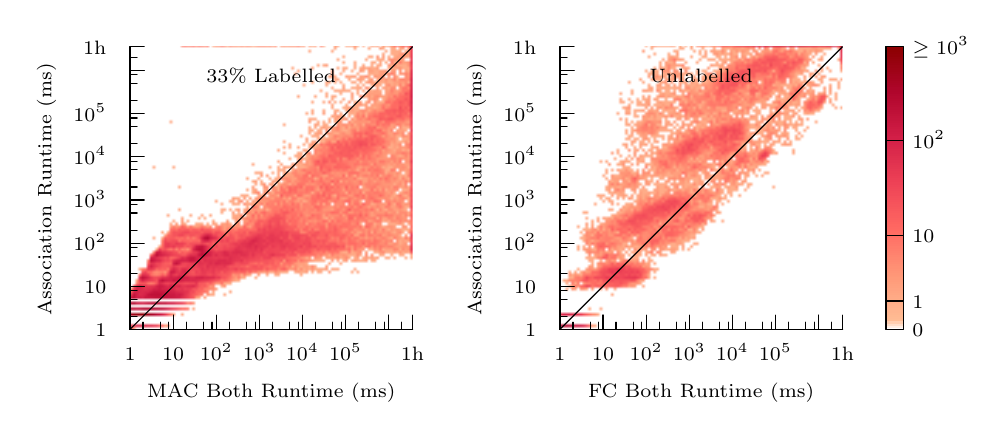
\begin{tikzpicture}[gnuplot]
%% generated with GNUPLOT 5.0p0 (Lua 5.2; terminal rev. 99, script rev. 100)
%% Tue 19 Apr 2016 16:47:19 AEST
\tikzset{every node/.append style={font={\scriptsize}}}
% \path (0.000,0.000) rectangle (10.922,7.366);
\gpcolor{color=gp lt color border}
\gpsetlinetype{gp lt border}
\gpsetdashtype{gp dt solid}
\gpsetlinewidth{1.00}
\draw[gp path] (1.320,5.785)--(1.320,2.197)--(4.908,2.197);
\node[gp node center,rotate=-270] at (0.246,3.991) {Association Runtime (ms)};
\node[gp node center] at (3.114,1.427) {MAC Both Runtime (ms)};
\begin{scope}
\clip (1.320,5.785) rectangle (4.908,2.197);
\def\gprawrgbimagedata{%
  ffffffffffffffffffffffffffffffffffffffffffffffffffffffffffffffffffffffffffffffffffffffffffffffff%
  ffffffffffffffffffff846eff6f65ff846eff7e6cff6f65ff8c72ff7367ff7e6cff8c72ff7869ffffffffac88ff9576%
  ff9576ff7869ff8c72ffac88ff846eff9576ff9576ff9f7dff8c72ff9f7dff8c72ff9576ffac88ff9f7dff8c72ff8c72%
  ff8c72ff9576ff8c72ff9f7dff8c72ffffffff9f7dff9576ff9f7dff9576ff9576ff9576ff7e6cff9f7dff9f7dffffff%
  ff9f7dffac88ff9f7dffffffff7e6cffac88ffffffffffffffffffff9f7dff9f7dffffffffffffffac88ffac88ffac88%
  ff9576ffac88ffffffffac88ffffffffffffff9f7dffac88ff9f7dffffffff9f7dffac88ff9f7dff9576ff6f65ff7869%
  ff7e6cfc6260fc6260ff6b63ac0527ffffffffffffffffffffffffffffffffffffffffffffffffffffffffffffffffff%
  ffffffffffffffffffffffffffffffffffffffffffffffffffffffffffffffffffffffffffffffffffffffffffffffff%
  ffffffffffffffffffffffffffffffffffffffffffffffffffffffffffffffffffffffffffffffffffffffffffffffff%
  ffffffffffffffffffffffffffffffffffffffffffffffffffffffffffffffffffffffffffffffffffffffffffffffff%
  ffffffffffffffffffffffffffffffffffffffffffffffffffffffffffffffffffffffffffffffffffffffac88ffffff%
  ffffffffffffffffffffffffffffffffac88ffffffffffffffffffffffffffac88ffffffffffffffffffff9f7dffac88%
  ffffffffffffffac88ffac88ffffffffac88ff9f7dffffffff9f7dee4156ffffffffffffffffffffffffffffffffffff%
  ffffffffffffffffffffffffffffffffffffffffffffffffffffffffffffffffffffffffffffffffffffffffffffffff%
  ffffffffffffffffffffffffffffffffffffffffffffffffffffffffffffffffffffffffffffffffffffffffffffffff%
  ffffffffffffffffffffffffffffffffffffffffffffffffffffffffffffffffffffffffffffffffffffffffffffffff%
  ffffffffffffffffffffffffffffffffffffffffffffffffffffffffffffffac88ffffffffffffffffffffffffffffff%
  ffffffffffffffac88ffffffffffffffffffffffffffffffffffffffffffffffffffffffffffffffffffffffffffffff%
  ffffffffffffffffffffffffffffffffac88ffffffffac88ffac88ffac88ffac88ffffffffac88ff9f7ded4155ffffff%
  ffffffffffffffffffffffffffffffffffffffffffffffffffffffffffffffffffffffffffffffffffffffffffffffff%
  ffffffffffffffffffffffffffffffffffffffffffffffffffffffffffffffffffffffffffffffffffffffffffffffff%
  ffffffffffffffffffffffffffffffffffffffffffffffffffffffffffffffffffffffffffffffffffffffffffffffff%
  ffffffffffffffffffffffffffffffffffffffffffffffffffffffffffffffffffffffffffffffffffffffffffffffff%
  ffffffffffffffffffffffffffffffffffffffffffffffffffffffffffffffffffffffffffffffffffffffffffffffff%
  ffffffffffffffffffffffffffffffffffffffffffffffffffffffffac88ffffffffffffffac88ffac88ffac88ff9f7d%
  ff8c72ff9f7dff9f7dec3f55ffffffffffffffffffffffffffffffffffffffffffffffffffffffffffffffffffffffff%
  ffffffffffffffffffffffffffffffffffffffffffffffffffffffffffffffffffffffffffffffffffffffffffffffff%
  ffffffffffffffffffffffffffffffffffffffffffffffffffffffffffffffffffffffffffffffffffffffffffffffff%
  ffffffffffffffffffffffffffffffffffffffffffffffffffffffffffffffffffffffffffffffffffffffffffffffff%
  ffffffffffffffffffffffffffffffffffffffffffffffffffffffffffffffffffffffffffffffffffffffffffffffff%
  ffac88ffffffffffffffffffffffffffffffffffffffffffffffffffac88ffac88ffffffff9576ffffffff9f7dffffff%
  ffac88ffffffffac88ff9f7dff9f7dff9576ff9f7dffac88e93c53ffffffffffffffffffffffffffffffffffffffffff%
  ffffffffffffffffffffffffffffffffffffffffffffffffffffffffffffffffffffffffffffffffffffffffffffffff%
  ffffffffffffffffffffffffffffffffffffffffffffffffffffffffffffffffffffffffffffffffffffffffffffffff%
  ffffffffffffffffffffffffffffffffffffffffffffffffffffffffffffffffffffffffffffffffffffffffffffffff%
  ffffffffffffffffffffffffffffffffffffffffffffffffffffffffffffffffffffffffffffffffffffffffffffffff%
  ffffffffffffffffffffac88ffffffffffffffffffffffffffffffffffffffffffffffffffffffffac88ffffffffffff%
  ffffffffac88ffac88ffac88ffffffff9f7dff8c72ff9576ff9f7dff9f7dff9f7dffffffffffffec4055ffffffffffff%
  ffffffffffffffffffffffffffffffffffffffffffffffffffffffffffffffffffffffffffffffffffffffffffffffff%
  ffffffffffffffffffffffffffffffffffffffffffffffffffffffffffffffffffffffffffffffffffffffffffffffff%
  ffffffffffffffffffffffffffffffffffffffffffffffffffffffffffffffffffffffffffffffffffffffffffffffff%
  ffffffffffffffffffffffffffffffffffffffffffffffffffffffffffffffffffffffffffffffffffffffffffffffff%
  ffffffffffffffffffffffffffffffffffffffffffffffffffffffffffffffac88ffffffffffffffffffffac88ffffff%
  ffffffffffffffffffffffffffac88ffac88ffffffffac88ffffffffac88ffffffff7e6cffac88ffac88ff7e6cff9f7d%
  ff9f7dff9576e33450ffffffffffffffffffffffffffffffffffffffffffffffffffffffffffffffffffffffffffffff%
  ffffffffffffffffffffffffffffffffffffffffffffffffffffffffffffffffffffffffffffffffffffffffffffffff%
  ffffffffffffffffffffffffffffffffffffffffffffffffffffffffffffffffffffffffffffffffffffffffffffffff%
  ffffffffffffffffffffffffffffffffffffffffffffffffffffffffffffffffffffffffffffffffffffffffffffffff%
  ffffffffffffffffffffffffffffffffffffffac88ffffffffac88ff9f7dffffffffffffffffffffffffffffffffffff%
  ffffffffffffffffffffac88ffffffffffffffac88ffffffffffffffac88ffffffffac88ffac88ffffffffffffff9576%
  ffac88ff846effac88ffac88ffac88ffac88ff9576ec3f55ffffffffffffffffffffffffffffffffffffffffffffffff%
  ffffffffffffffffffffffffffffffffffffffffffffffffffffffffffffffffffffffffffffffffffffffffffffffff%
  ffffffffffffffffffffffffffffffffffffffffffffffffffffffffffffffffffffffffffffffffffffffffffffffff%
  ffffffffffffffffffffffffffffffffffffffffffffffffffffffffffffffffffffffffffffffffffffffffffffffff%
  ffffffffffffffac88ffffffffffffffffffffffffffffffffffffffac88ffffffffffffffffffffffffffffffffffff%
  ffffffffffffffac88ffffffffac88ffac88ffffffffffffffac88ffffffffac88ff9f7dffac88ff9f7dffac88ffac88%
  ff9f7dffffffffffffffffffffac88ffac88ffac88ff9f7dff9576ffac88ffac88ffac88ee4156ffffffffffffffffff%
  ffffffffffffffffffffffffffffffffffffffffffffffffffffffffffffffffffffffffffffffffffffffffffffffff%
  ffffffffffffffffffffffffffffffffffffffffffffffffffffffffffffffffffffffffffffffffffffffffffffffff%
  ffffffffffffffffffffffffffffffffffffffffffffffffffffffffffffffffffffffffffffffffffffffffffffffff%
  ffffffffffffffffffffffffffffffffffffffffffffffffffffffffac88ffffffffffffffffffffffffffffffffffff%
  ffffffffffffffffffffffffffffffffac88ffffffffffffffffffffac88ffffffffffffffac88ffffffffffffff9576%
  ffac88ffffffff9f7dff9f7dffac88ffac88ff9f7dff9f7dff9576ffffffff9f7dff9576ffffffff9576ffffffff9f7d%
  ffac88e1314fffffffffffffffffffffffffffffffffffffffffffffffffffffffffffffffffffffffffffffffffffff%
  ffffffffffffffffffffffffffffffffffffffffffffffffffffffffffffffffffffffffffffffffffffffffffffffff%
  ffffffffffffffffffffffffffffffffffffffffffffffffffffffffffffffffffffffffffffffffffffffffffffffff%
  ffffffffffffffffffffffffffffffffffffffffffffffffffffffffffffffffffffffffffffffffac88ffffffffffff%
  ffffffffffffffffffffffffffffffffffffffffffffffffffffffffffffffac88ffffffffffffffac88ffffffffffff%
  ffffffffffffffffffffac88ffffffffffffffffffffac88ffac88ffac88ffac88ff9f7dff9f7dffac88ff8c72ff7e6c%
  ff9576ffffffff9576ff9576ff846eff9576de2e4dffffffffffffffffffffffffffffffffffffffffffffffffffffff%
  ffffffffffffffffffffffffffffffffffffffffffffffffffffffffffffffffffffffffffffffffffffffffffffffff%
  ffffffffffffffffffffffffffffffffffffffffffffffffffffffffffffffffffffffffffffffffffffffffffffffff%
  ffffffffffffffffffffffffffffffffffffffffffffffffffffffffffffffffffffffffffffffffffffffffffffffff%
  ffffffffffffffffffffffffffffffffffffffffffffffffffffffffffffffffffffffffffffffffffffffac88ffac88%
  ffac88ffffffffffffffffffff9f7dffac88ff9f7dff9f7dffffffff9f7dff9f7dff8c72ffac88ffffffff9576ff9f7d%
  ff9f7dff8c72ffffffff9576ffffffff8c72ffac88ffffffffffffff8c72ff9576dd2d4dffffffffffffffffffffffff%
  ffffffffffffffffffffffffffffffffffffffffffffffffffffffffffffffffffffffffffffffffffffffffffffffff%
  ffffffffffffffffffffffffffffffffffffffffffffffffffffffffffffffffffffffffffffffffffffffffffffffff%
  ffffffffffffffffffffffffffffffffffffffffffffffffffffffffffffffffffffffffffffffffffffffffffffffff%
  ffffffffffffffffffffffffffffffffffffffffffffffffffffffffffffffffffffffffffffffffffffffffffffffff%
  ffffffffffffffffffffffffffffffffac88ffac88ffffffffffffffffffffac88ffffffffffffff9f7dff9f7dffac88%
  ffffffffac88ff9576ffffffffac88ff9576ffac88ff9576ffac88ff9f7dff846effac88ff8c72ff846eff8c72ff8c72%
  d62449ffffffffffffffffffffffffffffffffffffffffffffffffffffffffffffffffffffffffffffffffffffffffff%
  ffffffffffffffffffffffffffffffffffffffffffffffffffffffffffffffffffffffffffffffffffffffffffffffff%
  ffffffffffffffffffffffffffffffffffffffffffffffffffffffffffffffffffffffffffffffffffffffffffffffff%
  ffffffffffffffffffffffffffffffffffffffffffffffffffffffffffffffffffffffffffffffffffffffffffffffff%
  ffffffffffffffac88ffffffffffffffffffffffffffac88ffac88ffffffffac88ffffffffac88ffffffffffffffffff%
  ffac88ffac88ffffffffac88ffffffffac88ff9576ff9f7dffac88ff9f7dffac88ffac88ff9f7dffac88ffac88ff9f7d%
  ff9f7dff9576ff9f7dff8c72ffac88da294bffffffffffffffffffffffffffffffffffffffffffffffffffffffffffff%
  ffffffffffffffffffffffffffffffffffffffffffffffffffffffffffffffffffffffffffffffffffffffffffffffff%
  ffffffffffffffffffffffffffffffffffffffffffffffffffffffffffffffffffffffffffffffffffffffffffffffff%
  ffffffffffffffffffffffffffffffffffffffffffffffffffffffffffffffffffffffffffffffffffffffffffffffff%
  ffffffffffffffffffffffffffac88ffffffffffffffffffffffffffffffffffffffffffffac88ffffffffffffffffff%
  ffffffffffffffac88ffffffffffffffffffffffffffac88ffffffffac88ffffffffffffffac88ff9576ffac88ffac88%
  ffffffff9f7dff8c72ffac88ff9f7dffac88ff846effac88ff846efe6862da294bffffffffffffffffffffffffffffff%
  ffffffffffffffffffffffffffffffffffffffffffffffffffffffffffffffffffffffffffffffffffffffffffffffff%
  ffffffffffffffffffffffffffffffffffffffffffffffffffffffffffffffffffffffffffffffffffffffffffffffff%
  ffffffffffffffffffffffffffffffffffffffffffffffffffffffffffffffffffffffffffffffffffffffffffffffff%
  ffffffffffffffffffffffffffffffffffffffffffffffffffffffffffffffffffffffffffffffffffffffffffffffff%
  ffffffffffffffffffffac88ffffffffffffffffffff9f7dffffffffffffffac88ffac88ffac88ff9f7dffffffff8c72%
  ffac88ffffffffffffff9f7dffffffff9f7dff9f7dffac88ff8c72ff8c72ffffffff9576ff7869ff7367ff8c72d7264a%
  ffffffffffffffffffffffffffffffffffffffffffffffffffffffffffffffffffffffffffffffffffffffffffffffff%
  ffffffffffffffffffffffffffffffffffffffffffffffffffffffffffffffffffffffffffffffffffffffffffffffff%
  ffffffffffffffffffffffffffffffffffffffffffffffffffffffffffffffffffffffffffffffffffffffffffffffff%
  ffffffffffffffffffffffffffffffffffffffffffffffffffffffffffffffffffffffffffffffffffffffffffffffff%
  ffffffffffffffffffffffffffac88ffffffffffffffffffffffffffac88ffac88ffac88ffac88ffac88ffac88ffffff%
  ffffffffac88ffffffffac88ffffffff9f7dffac88ff9f7dff9f7dffac88ffffffff9f7dff9f7dff7e6cff9576ff9f7d%
  ff9576ff7869ff7869ff6f65d62449ffffffffffffffffffffffffffffffffffffffffffffffffffffffffffffffffff%
  ffffffffffffffffffffffffffffffffffffffffffffffffffffffffffffffffffffffffffffffffffffffffffffffff%
  ffffffffffffffffffffffffffffffffffffffffffffffffffffffffffffffffffffffffffffffffffffffffffffffff%
  ffffffffffffffffffffffffffffffffffffffffffffffffffffffffffffffffffffffffffffffffffffffffffffffff%
  ffffffffffffffffffffffffffffffffffffffffffffffffffffffffffffffffffffac88ffffffffffffffffffffffff%
  ffac88ffffffffffffffffffff9f7dffffffffac88ffffffffffffffac88ff9f7dff9f7dff9f7dff9f7dff9f7dffffff%
  ff9f7dff9576ff8c72ff9576ff9576ff7869ff7e6cf6545cfc6260d52349ffffffffffffffffffffffffffffffffffff%
  ffffffffffffffffffffffffffffffffffffffffffffffffffffffffffffffffffffffffffffffffffffffffffffffff%
  ffffffffffffffffffffffffffffffffffffffffffffffffffffffffffffffffffffffffffffffffffffffffffffffff%
  ffffffffffffffffffffffffffffffffffffffffffffffffffffffffffffffffffffffffffffffffffffffffffffffff%
  ffffffffffffffffffffffffffffffffffffffac88ffffffffffffffffffffffffffffffffac88ffffffffffffffffff%
  ffac88ffffffffac88ffac88ffffffffffffffffffffffffffffffff9f7dffffffffffffff8c72ff9f7dffac88ff9576%
  ffac88ff9576ff8c72ff9f7dff9f7dff9f7dff8c72ff9576ff6f65ff846eff6f65ff6b63fd6561fd6561d21f47ffffff%
  ffffffffffffffffffffffffffffffffffffffffffffffffffffffffffffffffffffffffffffffffffffffffffffffff%
  ffffffffffffffffffffffffffffffffffffffffffffffffffffffffffffffffffffffffffffffffffffffffffffffff%
  ffffffffffffffffffffffffffffffffffffffffffffffffffffffffffffffffffffffffffffffffffffffffffffffff%
  ffffffffffffffffffffffffffffffffffffffffffffffffffffffffffffffffffffffffffffffffffffffffffffffff%
  ffffffffffffffffffffffffffffffffffffffffffffac88ffffffffffffffffffffac88ffffffffffffffac88ffffff%
  ffffffffffffffffffffffffff9f7dff9f7dff8c72ff9f7dffffffffac88ff9576ff7e6cff846eff846efe6862ff6b63%
  fe6862f7565cfc6260d8264affffffffffffffffffffffffffffffffffffffffffffffffffffffffffffffffffffffff%
  ffffffffffffffffffffffffffffffffffffffffffffffffffffffffffffffffffffffffffffffffffffffffffffffff%
  ffffffffffffffffffffffffffffffffffffffffffffffffffffffffffffffffffffffffffffffffffffffffffffffff%
  ffffffffffffffffffffffffffffffffffffffffffffffffffffffffffffffffffffffffffffffffffffffffffffffff%
  ffffffffffffffffffffffffffffffffac88ffffffffffffffffffffac88ffffffff9576ffffffffac88ffffffffac88%
  ffffffffffffff9576ffffffffac88ffac88ff9f7dffffffffac88ff8c72ffffffff9576ffac88ffac88ffac88ff7367%
  ff6f65ff7e6cfe6862fe6862f7585dfb605ffe6862f95c5ed32148ffffffffffffffffffffffffffffffffffffffffff%
  ffffffffffffffffffffffffffffffffffffffffffffffffffffffffffffffffffffffffffffffffffffffffffffffff%
  ffffffffffffffffffffffffffffffffffffffffffffffffffffffffffffffffffffffffffffffffffffffffffffffff%
  ffffffffffffffffffffffffffffffffffffffffffffffffffffffffffffffffffffffffffffffffffffffffffffffff%
  ffffffffffffffffffffffffffffffffffffffffffffffffffffffffffffffffffffffffffffffffffffffffffffffff%
  ffffffffac88ffffffffffffffffffffffffffac88ffffffffffffffac88ffac88ff9576ffac88ff9f7dffffffff9f7d%
  ff9f7dff9f7dff9576ff7e6cff8c72ff9576ff6f65ff6b63ff6b63fb605ffd6561ff6b63f85a5dda294bffffffffffff%
  ffffffffffffffffffffffffffffffffffffffffffffffffffffffffffffffffffffffffffffffffffffffffffffffff%
  ffffffffffffffffffffffffffffffffffffffffffffffffffffffffffffffffffffffffffffffffffffffffffffffff%
  ffffffffffffffffffffffffffffffffffffffffffffffffffffffffffffffffffffffffffffffffffffffffffffffff%
  ffffffffffffffffffffffffffffffffffffffffffffffffffffffffffffffffffffffffffffffffffffffffffffffff%
  ffffffffffffffffffffffffffffffffffffffac88ffffffffffffffffffffac88ffac88ff9f7dff9f7dffac88ffac88%
  ffffffffffffff9f7dff9f7dff9f7dffac88ff9f7dff9576ff6f65ff8c72ff7e6cff6b63fe6862ff6f65f34d59fe6862%
  f85a5dff6f65d7254affffffffffffffffffffffffffffffffffffffffffffffffffffffffffffffffffffffffffffff%
  ffffffffffffffffffffffffffffffffffffffffffffffffffffffffffffffffffffffffffffffffffffffffffffffff%
  ffffffffffffffffffffffffffffffffffffffffffffffffffffffffffffffffffffffffffffffffffffffffffffffff%
  ffffffffffffffffffffffffffffffffffffffffffffffffffffffffffffffffffffffffffffffffffffffffffffffff%
  ffffffffffffffffffffffffffac88ffffffffffffffffffffac88ffffffffffffffffffffac88ffac88ffffffffffff%
  ffac88ffac88ff9f7dffac88ffac88ff9576ff8c72ff9576ffac88ff9576ff846eff9576ff8c72ff846efa5e5ffb605f%
  fa5e5ff7585dfb605ff7565cf85a5dfe6862fc6260d8264affffffffffffffffffffffffffffffffffffffffffffffff%
  ffffffffffffffffffffffffffffffffffffffffffffffffffffffffffffffffffffffffffffffffffffffffffffffff%
  ffffffffffffffffffffffffffffffffffffffffffffffffffffffffffffffffffffffffffffffffffffffffffffffff%
  ffffffffffffffffffffffffffffffffffffffffffffffffffffffffffffffffffffffffffffffffffffffffffffffff%
  ffffffffffffffffffffffffffffffffffffffffffffac88ffffffffac88ffffffffffffffffffff9f7dffffffffffff%
  ffffffff9576ffffffffac88ffffffffffffffac88ffac88ffac88ff8c72ff9f7dff8c72ffac88ff8c72ff846eff7869%
  ff7e6cfd6561fd6561fd6561fa5e5ffd6561fa5e5fff6b63f85a5dfd6561fb605fff7e6ce1314fffffffffffffffffff%
  ffffffffffffffffffffffffffffffffffffffffffffffffffffffffffffffffffffffffffffffffffffffffffffffff%
  ffffffffffffffffffffffffffffffffffffffffffffffffffffffffffffffffffffffffffffffffffffffffffffffff%
  ffffffffffffffffffffffffffffffffffffffffffffffffffffffffffffffffffffffffffffffffffffffffffffffff%
  ffffffffffffffffffffffffffffffffffffffffffffffffffffffffffffffffffffffffffffffffffffffffffffffff%
  ffffffffffffffffffffffffffffffff9f7dffac88ff9576ffac88ffac88ffffffffac88ffffffff9f7dff7e6cff9576%
  ff7367ffac88ff7869ff7869fe6862ff6b63fc6260fd6561ff7367fe6862fc6260fe6862f85a5df7585dfe6862ff6f65%
  ff6b63e73952ffffffffffffffffffffffffffffffffffffffffffffffffffffffffffffffffffffffffffffffffffff%
  ffffffffffffffffffffffffffffffffffffffffffffffffffffffffffffffffffffffffffffffffffffffffffffffff%
  ffffffffffffffffffffffffffffffffffffffffffffffffffffffffffffffffffffffffffffffffffffffffffffffff%
  ffffffffffffffffffffffffffffffffffffffffffffffffffffffffffffffffffffffffffffffffffffffffffffffff%
  ffffffffffffffac88ffac88ffac88ffffffffffffffffffffffffffac88ffffffff9f7dffac88ffac88ff9f7dff9576%
  ffffffff9576ffac88ff8c72ff846eff9576ff846eff6f65ff846eff846eff7367f85a5dfb605ffc6260f7585df7565c%
  fd6561ff7367ff6f65fe6862ff7e6cff846eef4356ffffffffffffffffffffffffffffffffffffffffffffffffffffff%
  ffffffffffffffffffffffffffffffffffffffac88ffffffffffffffffffffffffffffffffffffffffffffffffffffff%
  ffffffffffffffffffffffffffffffffffffffffffffffffffffffffffffffffffffffffffffffffffffffffffffffff%
  ffffffffffffffffffffffffffffffffffffffffffffffffffffffffffffffffffffffffffffffffffffffffffffffff%
  ffffffffffffffffffffffffffffffffffffffffffff9f7dffffffffffffffac88ffffffffac88ffffffffac88ffffff%
  ffac88ff9f7dff9576ffffffffffffff8c72ffac88ff9576ff9576ff9576ff9576ff9576ff9f7dff7e6cff846efe6862%
  ff7869ff8c72fe6862ff6b63ff7367ff7869ff8c72ff846eff846eff9576ff9f7de83b53ffffffffffffffffffffffff%
  ffffffffffffffffffffffffffffffffffffffffffffffffffffffffffffffffffffffffffffffffffffffffffffffff%
  ffffffffffffffffffffffffffffffffffffffffffffffffffffffffffffffffffffffffffffffffffffffffffffffff%
  ffffffffffffffffffffffffffffffffffffffffffffffffffffffffffffffffffffffffffffffffffffffffffffffff%
  ffffffffffffffffffffac88ffffffffffffffffffffffffffffffffffffffffffffffffffffffffffffff9f7dffac88%
  ffffffffac88ffac88ffffffffffffffffffff9576ff9f7dff8c72ff9576ff9f7dff846effac88ff9576ff8c72ffac88%
  ff7e6cff7e6cff8c72ff8c72ff6b63ff846eff6f65ff7869ff7367ff9f7dff9576ff7e6cff846eff9f7dff8c72ff8c72%
  ed4155ffffffffffffffffffffffffffffffffffffffffffffffffffffffffffffffffffffffffffffffffffffffffff%
  ffffffffffffffffffffffffffffffffffffffffffffffffffffffffffffffffffffffffffffffffffffffffffffffff%
  ffffffffffffffffffffffffffffffffffffffffffffffffffffffffffffffffffffffffffffffffffffffffffffffff%
  ffffffffffffffffffffffffffffffffffffffffffffffffffffffffffffffffffffffffffffffffffffffffffffffff%
  ffffffffac88ffffffffac88ffffffffac88ff9f7dffac88ffac88ff9f7dff9576ff846eff9f7dffac88ff8c72ffac88%
  ff9576ff9576ff9f7dff846eff8c72ff7e6cfe6862ff6f65fc6260ff9576ff8c72ff846eff7e6cff9576ff9f7dff9576%
  ffffffff8c72ffac88ffac88ffac88f24a59ffffffffffffffffffffffffffffffffffffffffffffffffffffffffffff%
  ffffffffffffffffffffffffffffffffffffffffffffffffffffffffffffffffffffffffffffffffffffffffffffffff%
  ffffffffffffffffffffffffffffffffffffffffffffffffffffffffffffffffffffffffffffffffffffffffffffffff%
  ffffffffffffffffffffffffffffffffffffffffffffffffffffffffffffffffffffffffffffffffffffffffffffffff%
  ffffffffffffffffffffffffffffffffffffffac88ffac88ffffffffac88ffac88ffffffff8c72ffffffff9f7dff9576%
  ff8c72ff9f7dffac88ffac88ff9f7dff846eff7869ff9f7dff7e6cff7e6cff7367ff6f65fd6561ff7e6cfe6862fe6862%
  ff9576ff8c72ff9f7dff846effffffff9f7dff9f7dff9f7dffac88ffffffe93c53ffffffffffffffffffffffffffffff%
  ffffffffffffffffffffffffffffffffffffffffffffffffffffffffffffffffffffffffffffffffffffffffffffffff%
  ffffffffffffffffffffffffffffffffffffffffffffffffffffffffffffffffffffffffffffffffffffffffffffffff%
  ffffffffffffffffffffffffffffffffffffffffffffffffffffffffffffffffffffffffffffffffffffffffffffffff%
  ffffffffffffffffffffffffffffffffffffffffffffffffffffffffffffffffffffac88ffffffffac88ff9f7dff9f7d%
  ffffffff9f7dff9576ff9f7dffac88ffac88ff9576ff8c72ff9f7dff9f7dff846efe6862ff6b63fd6561ff7367f95c5e%
  fe6862ff6f65ff846eff7e6cff7869ff6b63ff846eff9f7dff9f7dff846eff8c72ff9f7dff8c72ffffffff9f7df34d59%
  ffffffffffffffffffffffffffffffffffffffffffffffffffffffffffffffffffffffffffffffffffffffffffffffff%
  ffffffffffffffffffffffffffffffffffffffffffffffffffffffffffffffffffffffffffffffffffffffffffffffff%
  ffffffffffffffffffffffffffffffffffffffffffffffffffffffffffffffffffffffffffffffffffffffffffffffff%
  ffffffffffffffffffffffffffffffffffffffffffffffffffffffffffffffffffffffffffffffffac88ffffffffffff%
  ffffffffac88ffac88ffac88ffffffffac88ffffffffac88ff9f7dff7e6cff8c72ff9576ff8c72ff846eff8c72ff8c72%
  fd6561ff7e6cfc6260ff846eff7869fd6561f95c5ef95c5eff6f65ff7e6cff9f7dff846eff9576ff9f7dff9576ffac88%
  ffac88ff8c72ff9576ff9f7def4457ffffffffffffffffffffffffffffffffffffffffffffffffffffffffffffffffff%
  ffffffffffffffffffffffffffffffffffffffffffffffffffffffffffffffffffffffffffffffffffffffffffffffff%
  ffffffffffffffffffffffffffffffffffffffffffffffffffffffffffffffffffffffffffffffffffffffffffffffff%
  ffffffffffffffffffffffffffffffffffffffffffffffffffffffffffffffffffffffffffffffffffffffffffffffff%
  ffffffffffffffffffffffffff9f7dffffffffffffffffffffac88ffac88ffac88ff9f7dff9f7dff9576ff8c72ff9f7d%
  ff8c72ff7367ff8c72fe6862ff7367ff6b63fb605ffc6260fe6862f85a5dfd6561f7565cff6f65fe6862ff6f65ff7869%
  ff8c72ff9576ff8c72ff9576ffac88ffffffffac88ffac88ff9f7df14858ffffffffffffffffffffffffffffffffffff%
  ffffffffffffffffffffffffffffffffffffffffffffffffffffffffffffffffffffffffffffffffffffffffffffffff%
  ffffffffffffffffffffffffffffffffffffffffffffffffffffffffffffffffffffffffffffffffffffffffffffffff%
  ffffffffffffffffffffffffffffffffffffffffffffffffffffffffffffffffffffffffffffffffffffffffffffffff%
  ffffffffac88ffffffffffffffffffffffffffffffffffffffffffffac88ffffffffac88ff9f7dffffffffac88ffac88%
  ff8c72ff7869ff9f7dff9f7df95c5eff7869fe6862fd6561ff7367fa5e5ff95c5ef7565cf5515bf6545cf7585dfc6260%
  fb605fff6f65fc6260ff6f65ff6b63ff846eff8c72ff9f7dff9576ffac88ffac88ffac88ff9576ffac88ef4356ffffff%
  ffffffffffffffffffffffffffffffffffffffffffffffffffffffffffffffffffffffffffffffffffffffffffffffff%
  ffffffffffffffffffffffffffffffffffffffffffffffffffffffffffffffffffffffffffffffffffffffffffffffff%
  ffffffffffffffffffffffffffffffffffffffffffffffffffffffffffffffffffffffffffffffffffffffffffffffff%
  ffffffffffffffffffffffffffffffffffffffffffffffffffac88ffffffffffffffffffffffffffac88ffffffffac88%
  ff9576ffac88ffac88ff7367ff846eff7367fe6862ff6f65fb605ffd6561f95c5eff6f65f7585dff6b63f95c5ef85a5d%
  f7565cf24a59f5535bf4505aff6b63f7585dfa5e5fff6f65ff6b63ff7e6cff8c72ff8c72ffac88ff9f7dff9f7dff8c72%
  ffffffff8c72ff846ef14958ffffffffffffffffffffffffffffffffffffffffffffffffffffffffffffffffffffffff%
  ffffffffffffffffffffffffffffffffffffffffffffffffffffffffffffffffffffffffffffffffffffffffffffffff%
  ffffffffffffffffffffffffffffffffffffffffffffffffffffffffffffffffffffffffffffffffffffffffffffffff%
  ffffffffffffffffffffffffffffffffffffffffffffffffffffffffffffffffffffac88ffffffffac88ffffffffffff%
  ffac88ffffffffffffffffffffac88ffac88ffac88ff9576ff9576ff7e6cff8c72ff7367f95c5eff7869f85a5dfb605f%
  fb605ff85a5df85a5dfc6260f6545cfa5e5ff7585dfd6561fa5e5ffc6260ff6b63ff7869ff7e6cff8c72fd6561ff846e%
  ffac88ffac88ff9f7dffac88ff9576ff9f7dff9576ff846ef7585dffffffffffffffffffffffffffffffffffffffffff%
  ffffffffffffffffffffffffffffffffffffffffffffffffffffffffffffffffffffffffffffffffffffffffffffffff%
  ffffffffffffffffffffffffffffffffffffffffffffffffffffffffffffffffffffffffffffffffffffffffffffffff%
  ffffffffffffffffffffffffffffffffffffffffffffffffffffffffffffffffffffffffffffffffffffffac88ffffff%
  ffffffffffffffffffffffffffffffffffffffffffff9f7dffac88ffffffffffffff846eff8c72ff7e6cff846eff7e6c%
  ff6f65fb605ffe6862ff6b63fc6260f95c5efb605ff85a5df7585dfa5e5ffd6561fe6862fb605ffd6561fe6862ff6b63%
  ff6f65ff846eff7e6cff9f7dff8c72ff9576ff9f7dffac88ff9576ff9576ffac88ff9f7dffac88f24b59ffffffffffff%
  ffffffffffffffffffffffffffffffffffffffffffffffffffffffffffffffffffffffffffffffffffffffffffffffff%
  ffffffffffffffffffffffffffffffffffffffffffffffffffffffffffffffffffffffffffffffffffffffffffffffff%
  ffffffffffffffffffffffffffffffffffffffffffffffffffffffffffffffffffffffffffffffffffffffffffffffff%
  ffffffffffffffffffffffffffffffffac88ffffffffffffffffffffffffffac88ffac88ffffffff9f7dff846effffff%
  ff846eff9576ff8c72ff7869ff7e6cff7367ff7367fa5e5ffc6260f7585dfb605ffb605ff95c5efe6862fc6260fb605f%
  ff7869ff6b63fe6862ff7367ff7869ff8c72ff9576ff7e6cff9576ff9576ff9f7dff9f7dff9f7dff8c72ff8c72ff7869%
  ff846eff9576f04557ffffffffffffffffffffffffffffffffffffffffffffffffffffffffffffffffffffffffffffff%
  ffffffffffffffffffffffffffffffffffffffffffffffffffffffffffffffffffffffffffffffffffffffffffffffff%
  ffffffffffffffffffffffffffffffffffffffffffffffffffffffffffffffffffffffffffffffffffffffffffffffff%
  ffffffffffffffffffffffffffffffffffffffffffffffffffffffffffffffffffffffffffffffffffffffac88ffac88%
  ffac88ffffffffac88ff9f7dff8c72ff9576ff846eff7367ff6f65ff7e6cf95c5efc6260fe6862fd6561fc6260fb605f%
  f95c5ef95c5ef95c5eff6f65fd6561ff8c72fd6561ff7e6cff6f65ff846eff8c72ff7869ff8c72ff9576ff9f7dffffff%
  ff846eff8c72ff9f7dffac88ff9f7dff846eff9f7df5515bffffffffffffffffffffffffffffffffffffffffffffffff%
  ffffffffffffffffffffffffffffffffffffffffffffffffffffffffffffffffffffffffffffffffffffffffffffffff%
  ffffffffffffffffffffffffffffffffffffffffffffffffffffffffffffffffffffffffffffffffffffffffffffffff%
  ffffffffffffffffffffffffffffffffffffffffffffffffffffffffffffffffffffffffffffffffffffffffffffffff%
  ffffffffac88ffffffffffffffac88ff9576ffac88ffac88ff9576ff846eff846eff7e6cff7367fb605ffe6862ff6b63%
  fc6260fd6561ff846efb605fff8c72ff7e6cfb605fff6f65ff7869ff8c72ff7869ff6f65ff846eff6f65ff7e6cff846e%
  ff9576ff9576ff9576ff9576ff9576ff846eff846eff9576ff846eff9576ff9576ff9f7df24a59ffffffffffffffffff%
  ffffffffffffffffffffffffffffffffffffffffffffffffffffffffffffffffffffffffffffffffffffffffffffffff%
  ffffffffffffffffffffffffffffffffffffffffffffffffffffffffffffffffffffffffffffffffffffffffffffffff%
  ffffffffffffffffffffffffffffffffffffffffffffffffffffffffffffffffffffffffffffffffffffffffffffffff%
  ffffffffffffffac88ffffffffffffffffffffffffffffffffffffff9f7dff9576ffffffff9576ff9f7dff846efe6862%
  f7565cff6f65f7565cf95c5eff7367fc6260fa5e5fff7367fe6862ff7869ff7869ff7e6cff7e6cff846eff7367ff9576%
  ff7e6cff7e6cff8c72ff846eff846eff9576ff7869ff7869ff8c72ff8c72ff9f7dff846eff9576ff7869ffffffff9576%
  ff9576e93c53ffffffffffffffffffffffffffffffffffffffffffffffffffffffffffffffffffffffffffffffffffff%
  ffffffffffffffffffffffffffffffffffffffffffffffffffffffffffffffffffffffffffffffffffffffffffffffff%
  ffffffffffffffffffffffffffffffffffffffffffffffffffffffffffffffffffffffffffffffffffffffac88ffffff%
  ffffffffffffffffffffffffffffffffffffffffffffffffffac88ffffffffffffffffffff9f7dff9f7dffac88ffac88%
  ff9f7dff9576ff9f7dff8c72fe6862fd6561fd6561fc6260ff7367ff7367ff7869ff7869fd6561ff6b63ff6b63ff7367%
  ff7e6cff846eff7367ff7869ff846eff7869ff7869ff846eff9f7dff7367ff8c72ff8c72ff8c72ff9576ff9f7dff9576%
  ff9f7dff8c72ff9576ff9576ff9f7dff9f7df34d59ffffffffffffffffffffffffffffffffffffffffffffffffffffff%
  ffac88ffffffffffffffffffffffffffffffffffffffac88ffffffffffffffffffffffffffffffffffffffffffffffff%
  ffffffffffffffffffffffffffffffffffffffffffffffffffffffffffffffffffffffffffffffffffffffffffffffff%
  ffffffffffffffffffffffffffffffffffffffffffffffffffffffffac88ffffffffffffffac88ffffffff9f7dffac88%
  ffac88ff9f7dffffffffac88ffac88ffac88ff9f7dff8c72ff846eff7e6cff9576f85a5dff6f65ff6b63ff6b63ff7869%
  fc6260fd6561fe6862ff6b63fd6561ff6b63ff846eff7e6cff9576ff9f7dff8c72ff9576ff8c72ff7869ff8c72ff7e6c%
  ff8c72ffac88ff9f7dffac88ffac88ff9576ff9576ff9576ff8c72ff9576ffac88f4505affffffffffffffffffffffff%
  ffffffffffffffffffffffffffffffffffffffffffffffffffffffffffffffffffffffffffffffffffffffffffffffff%
  ffffffffffffffffffffffffffffffffffffffffffffffffffffffffffffffffffffffffffffffffffffffffffffffff%
  ffffffffffffffffffffffffffffffffffffffffffffffffffffffffffffffffffffffffffffffffffffffffffffffff%
  ffffffffac88ffac88ffac88ffffffffffffffac88ff8c72ff9f7dff8c72ff7367ff846eff846eff7e6cff7869ff8c72%
  fc6260ff7e6cff7367fb605fff7869ff7e6cff7367ff7e6cff7367ff7869ff8c72ff7e6cff8c72ffac88ff8c72ff7869%
  ff9576ff7367ff846eff7367ff7367ff7e6cff8c72ffac88ffac88ff7869ff846effffffff9576ff9576ff9f7dff9576%
  f14958ffffffffffffffffffffffffffffffffffffffffffffffffffffffffffffffffffffffffffffffffffffffffff%
  ffffffffffffffffffffffffffffffffffffffffffffffffffffffffffffffffffffffffffffffffffffffffffffffff%
  ffffffffffffffffffffffffffffffffffffffffffffffffffffffffffffffffffffffffffffffffffffffac88ffac88%
  ffac88ffffffffffffffffffffac88ffffffffac88ffffffffac88ff9f7dffac88ff8c72ff846eff9576ff9576ff9576%
  ff7869ff6b63ff846eff7869ff7e6cff7e6cfb605fff7367ff7e6cff9576ff8c72ff9576ff8c72ff8c72ff9576ff7367%
  ff6f65ff6f65ff7367ff8c72ff9576ff9576ff9f7dff7e6cff846eff7e6cff7e6cff846effac88ff9576ff9576ff9f7d%
  ff8c72ff9f7dffffffffac88ff9576ef4457ffffffffffffffffffffffffffffffffffffffffffffffffffffffffffff%
  ffffffffffffffffffffffffffffffffffffffffffffffffffffffffffffffffffffffffffffffffffffffffffffffff%
  ffffffffffffffffffffffffffffffffffffffffffffffffffffffffffffffffffffffffffffffffffffffffffffffff%
  ffffffffffffffffffffffffffffffff9f7dffffffff9f7dffffffffffffffffffffac88ffffffff9f7dffac88ff9f7d%
  ff9f7dff846eff846eff8c72ff7367ff6f65ffac88ff6b63ff7869ff7869ff8c72ff9f7dff9f7dff7e6cff7e6cff8c72%
  ff8c72ff9576fe6862ffac88ff7869ff8c72ffac88ff7e6cff9576ff846eff7e6cff8c72ff7e6cff8c72ff7367ffac88%
  ff8c72ff8c72ff7869ff8c72ff9f7dff9576ffac88ff9f7dffac88ff846ef24a59ffffffffffffffffffffffffffffff%
  ffffffffffffffffffffffffffffffffffffffffffffffffffffffffffffffffffffffffffffffffffffffffffffffff%
  ffffffffffffffffffffffffffffffffffffffffffffffffffffffffffffffffffffffffffffffffffffffffffffffff%
  ffffffffffffffffffffffffffffffffac88ffffffffffffffffffffac88ffffffffffffffffffffac88ffffffffac88%
  ffac88ff846eff9576ff8c72ff9576ff9f7dff9f7dff846eff7e6cff7367ff7e6cff7869ff7e6cffac88ff9576ff6f65%
  ff9576ff7e6cff846eff9576ff7e6cff7e6cff7e6cff846eff7e6cff8c72ff8c72ff7869ff9f7dffac88ff9f7dff9f7d%
  ff8c72ff9576ff846eff9576ff7869ff8c72ff6f65ff846eff9576ff846eff9576ffac88ff846eff9f7dffac88f14958%
  ffffffffffffffffffffffffffffffffffffffffffffffffffffffffffffffffffffffffffffffffffffffffffffffff%
  ffffffffffffffffffffffffffffffffffffffffffffffffffffffffffffffffffffffffffffffffffffffffffffffff%
  ffffffffffffffffffffffffffffffffffffffffffffffffffffffffffffffffffffffffffac88ff9f7dffffffffac88%
  ffffffffffffffffffff9f7dffac88ffac88ffffffffac88ff8c72ff846eff9f7dff8c72ff8c72ff7e6cff7869ff7869%
  ff8c72ff6f65ff846eff7e6cff6f65ff7e6cff8c72ff846efb605fff7e6cff6b63ffac88ff846eff9576ff846eff8c72%
  ff9576ff8c72ff7869ff9f7dff9f7dff846eff8c72ff9f7dff8c72ff8c72ff9576ff846eff846eff9576ff9576ff9f7d%
  ff9576ff9f7dff7e6cff9f7df24a59ffffffffffffffffffffffffffffffffffffffffffffffffffffffffffffffffff%
  ffffffffffffffffffffffffffffffffffffffffffffffffffffffffffffffffffffffffffffffffffffffffffffffff%
  ffffffffffffffffffffffffffffffffffffffffffffffffffffffffffffffffffffffffffffffffffffffffffffffff%
  ffffffffffffffac88ffffffffac88ff9576ffffffff9f7dffac88ffffffffac88ff9f7dff8c72ff9576ffac88ff8c72%
  ff9576ff7367ff7367ff7869ff9576ff8c72ff9576ff8c72ff7e6cff846efe6862ff7869ff7367ffac88ff6f65ff7e6c%
  ff7e6cff7e6cff846eff7e6cff846eff8c72ff8c72ff7869ff9576ff846eff846eff8c72ff846eff7e6cff8c72ff9576%
  ff9576ff9576ff9576ffac88ff9576ff8c72ffac88ff846efffffff85a5dffffffffffffffffffffffffffffffffffff%
  ffffffffffffffffffffffffffffffffffffffffffffffffffffffffffffffffffffffffffac88ffffffffffffffffff%
  ffffffffffffffffffffffffffffffffffffffffffffffffffffffffffffffffffffffffffffffffffffffffffffffff%
  ffffffffffffffffffffffffffffffffffffff9f7dffffffffffffffffffff9576ff9576ffffffff846eff9f7dffac88%
  ff7869ff9576ff7e6cfe6862ff7869fe6862ff7367fd6561ff9576ff7367ff7367ff7367ff846eff9576fa5e5fff7e6c%
  fb605fff7367fe6862ff846eff6f65ff846eff8c72fd6561ff8c72ff7869ff846eff6f65ffffffff9f7dff8c72ff846e%
  ff7e6cff7869ff9576ff9576ff8c72ff9576ff8c72ff9f7dff7e6cff846eff9f7dff9f7dff8c72ffac88f85a5dffffff%
  ffffffffffffffffffffffffffffffffffffffffffffffffffffffffffffffffffffffffffffffffffffffffffffffff%
  ffffffffffffffffffffffffffffffffffffffffffffffffffffffffffffffffffffffffffffffffffffffffffffffff%
  ffffffffffffffffffffffffffffffffffffffffffffffffffffffffac88ffffffffac88ff9f7dffffffffffffffac88%
  ff9576ffffffff9576ff8c72ffac88ff7367ff7869ff9576fc6260ff6b63fe6862ff846eff846eff846eff6f65ff7869%
  ff6f65ff8c72ff9f7dff7e6cff846efd6561ff6b63ff846eff7869ff7e6cff7e6cff9f7dff7869ff846eff7e6cff846e%
  ff8c72ff846eff9576ff9f7dff9576ff6f65ff9f7dff846eff9f7dff7e6cffac88ff9576ff9576ff8c72ff8c72ffffff%
  ffac88ffac88ff9f7df24b59ffffffffffffffffffffffffffffffffffffffffffffffffffffffffffffffffffffffff%
  ffffffffffffffffffffffffffffffffffffffffffffffffffffffffffffffffffffffffffffffffffffffffffffffff%
  ffffffffffffffffffffffffffffffffffffffffffffffffffffffffffffffffffffffffffffffffffffffffffffffff%
  ffac88ff9576ff846effffffff9576ff9576ff9576ffac88ff846eff846eff7e6cff6b63ff7367fe6862ff7869ff6f65%
  ff7e6cff7869ff7e6cff7869ff846effac88ff846eff7367ff9576fd6561ff7869ff7367ff6f65ff7869ff7869ff846e%
  ff846effac88ff7367ff8c72ff846eff8c72ff7367ffac88ff846eff7e6cff846eff7869ff7869ff846eff846eff9576%
  ff9f7dff8c72ffac88ffffffffac88ff9576ff846eff9576f7565cffffffffffffffffffffffffffffffffffffffffff%
  ffffffffffffffffffffffffffffffffffffffffffffffffffffffffffffffffffffffffffffffffffffffffffffffff%
  ffffffffffffffffffffffffffffffffffffffffffffffffffffffffffffffffffffffffffffffffffffffffffffffff%
  ffffffffac88ffac88ffac88ffffffffffffffffffffac88ffac88ff9576ffffffff9576ff8c72ff9576ffac88fa5e5f%
  ff846eff7367ff7e6cff846eff9f7dff6f65ff7367ff9576ff9f7dff9576ff7869ff7869fd6561ff7367fb605fff846e%
  fe6862ff9576ffac88ff7367ff7e6cff7869ff7e6cff9576ff9576ff7869ff6f65ff846eff6f65ff9576ff7869ff7e6c%
  ff846eff846eff6b63ff7e6cff9576ff8c72ff9f7dffac88ff9576ff7869ff9f7dffac88ff9576f34e5affffffffffff%
  ffffffffffffffffffffffffffffffffffffffffffffffffffffffffffffffffffffffffffffffffffffffffffffffff%
  ffffffffffffffffffffffffffffffffffffffffffffffffffffffffffffffffffffffffffffffffffffffffffffffff%
  ffffffffffffffffffff9f7dffac88ffac88ffffffff9f7dffffffff9f7dffffffff9f7dff9576ff846eff9576ff8c72%
  ff9576ff9f7dff846eff846eff7e6cff9f7dff8c72ffac88ff7869ff7e6cff9f7dff9f7dff9576ff846eff8c72ff6f65%
  ff7367ff6b63ff7367ff846eff6b63fe6862ff846eff8c72ff6b63ff9576ff9f7dff9576ff7869ff846eff9576ff846e%
  ff846eff7869ff8c72ff7869ff6f65ff7e6cff8c72ff9576ff9576ff8c72ff9576ffac88ff9576ff9f7dff8c72ff846e%
  ff9576ffac88f5535bffffffffffffffffffffffffffffffffffffffffffffffffffffffffffffffffffffffffffffff%
  ffffffffffffffffffffffffffffffffffffffffffffffffffffffffffffffffffffffffffffffffffffffffffffffff%
  ffffffffffffffac88ffffffffffffffffffffffffffac88ffac88ffffffff9f7dff8c72ffffffffac88ffffffff9f7d%
  ffac88ff8c72ff9f7dff9576ff9576ff846eff846eff7e6cff7869ff8c72ff7869ff9f7dff846eff7e6cff9576ff9f7d%
  ff8c72ffac88ff9f7dff846eff7367ff6b63ff846eff7869ff6f65ff7367ff9576ff846eff7367ff846eff8c72ff7e6c%
  fe6862ff6b63ff9576ff7e6cff7e6cffac88ffffffff846eff7e6cff8c72fe6862ff6f65ff7e6cffffffff8c72ff846e%
  ff9576ff846eff9576ff8c72ff9576ffffffffac88f24b59ffffffffffffffffffffffffffffffffffffffffffffffff%
  ffffffffffffffffffffffffffffffffffffffffffffffffffffffffffffffffffffffffffffffffffffffffffffffff%
  ffffffffffffffffffffffffffffffffffffffffffffffffffffffffac88ffffffffffffffffffffac88ffac88ffac88%
  ffffffff8c72ffac88ff9f7dffac88ff9f7dff9f7dff7e6cff9f7dff7869ff846eff7e6cff9f7dff7367ff9576ff7869%
  ff7e6cff8c72ff6b63ff846eff7869ff9f7dff7e6cff846eff8c72ff7367ff7e6cff9f7dff7367ffac88ff7869ff846e%
  ffffffff8c72ff8c72ff8c72ff846effffffff7869ff9576ff7367ff7367ff9576fd6561ff7e6cff846effac88ff9f7d%
  ff8c72ff9576ff9576ff9f7dff6f65ff9576ffac88ff7869ff846eff9f7dff9576ff9576f6545cffffffffffffffffff%
  ffffffffffffffffffffffffffffffffffffffffffffffffffffffffffffffffffffffffffffffffffffffffffffffff%
  ffffffffffffffffffffffffffffffffffffffffffffffffffffffffffffffffffffffffffffffffffffffffffffffff%
  ffffffffffffffffffffffffffffffffffffffffffffac88ffffffff7367ff7e6cff9576ffffffff8c72ff8c72ff7e6c%
  ff7e6cff7869ff7e6cff846eff6b63ff7367ff7869ff7869ff7869ff7367ff9576ff846eff846eff846eff8c72fe6862%
  ff6b63ff7869ff846eff8c72ff9576ff9576ff846eff9576ff7e6cff846eff846eff846eff7367ff9576ff7e6cff6b63%
  ff846eff8c72ff9f7dff8c72ff9576ff846eff9576ff9f7dff7e6cff846eff9f7dff9f7dff8c72ff7869ff9576ffac88%
  ffac88f04557ffffffffffffffffffffffffffffffffffffffffffffffffffffffffffffffffffffffffffffffffffff%
  ffffffffffffffffffffffffffac88ffffffffffffffffffffffffffffffffffffffffffffffffffffffffffffffffff%
  ffffffffffffffffffffac88ffac88ffffffffac88ffffffffac88ff9576ffffffffac88ff9576ff9f7dff9576ff9576%
  ff9f7dff9f7dff8c72ffac88ff9576ff7869ff7869ff7869fd6561ff7869ff6b63ff7869fb605fff846eff7869ff8c72%
  ff7e6cff8c72ff846eff7e6cff8c72ff6f65ff7e6cff9576ff9576ff9576ff9f7dff846eff7869ff846eff9576ff7869%
  f85a5dff846eff7869ff7869ff846eff846eff7869ff846eff6f65ff8c72ffac88ff846eff9f7dffac88ff8c72ff8c72%
  ff9f7dff9f7dff9576ff9f7dffac88fffffff95c5effffffffffffffffffffffffffffffffffffffffffffffffffffff%
  ffffffffffffffffffffffffffffffffffffffffffffffffffffffffffffffffffffffffffffffffffffffffffffffff%
  ffffffffffffffffffffffffffffffffffffffffffffffffffac88ffffffffffffffffffff9f7dffffffffac88ffffff%
  ff9f7dff846eff8c72ff9f7dff6f65ff9576ff7367fe6862ff7e6cff846eff7869ff6b63ff7367fd6561f85a5df85a5d%
  ff6b63ff7367ff7367ff7e6cff7869ff8c72ff8c72ff846eff8c72ff8c72ff846eff846eff8c72ff846eff7e6cff6b63%
  ff6f65ff7367ff9576ff7869ff6f65ff9576ff9576ff7e6cff846eff7367ff8c72ff7e6cff8c72ff9f7dff8c72ff9576%
  ff9576ff9576ff846eff9f7dff9576ff8c72ffac88ff8c72ff8c72ff8c72ffac88ff6b63ffffffffffffffffffffffff%
  ffffffffffffffffffffffffffffffffffffffffffffffffffffffffffffffac88ffffffffffffffffffffffffffffff%
  ffffffffffffffac88ffffffffffffffffffffac88ffffffffffffffac88ffffffffffffffffffffffffffffffffffff%
  ffffffffac88ffac88ffac88ff8c72ffffffffac88ff9576fe6862ff9576ff6f65ff9576ff7367ff7e6cff6f65ff6f65%
  f7585df7585dfd6561fa5e5fff7367ff7869ff6f65ff6f65ff846efe6862ff846eff9576ff8c72fe6862ff7869ff7367%
  ff7e6cff9f7dff7e6cff9576ff8c72ff8c72ff8c72ff7869ff9f7dff846eff6b63ff6f65ff7367ff7869fb605fff846e%
  ff6b63ff8c72ff9f7dff9576ff7e6cff7e6cff846eff7367ff7e6cff7e6cff9576ff8c72ff8c72ff9f7dff846eff9f7d%
  fa5e5fffffffffffffffffffffffffffffffffffffffffffffffffffffffffffffffffffffffffffffffffffffffffff%
  ffffffffffffffffffffffffffac88ffffffffffffffffffffffffffffffffac88ffffffffac88ffffffffffffffffff%
  ffffffffffffffffffffffffffffffffffffffac88ff9f7dffac88ff9576ff9576ff846eff8c72ff7869ff9576ff7367%
  ff846eff7e6cff6f65fb605ff5515bf4505af4505af5535bf95c5eff6f65ff7869fe6862ff7869ff6f65ff846eff7e6c%
  ff846eff6f65ff7e6cff846eff7367ff7e6cff9f7dffac88ff846eff9f7dff846eff7e6cff7e6cff846eff9576fd6561%
  fd6561ff9576ff7367ff7869ff7869ff8c72ff846eff846eff7e6cffac88ff7e6cff9f7dff9f7dff846eff8c72ff9f7d%
  ff7e6cff8c72ff9576ff9576fffffffe6862ffffffffffffffffffffffffffffffffffffffffffffffffffffffffffff%
  ffffffffffffffffffffffffffffffffffffffac88ffffffffffffff9f7dffffffffac88ffffffffffffffffffffffff%
  ffffffffffffffffffffffffffac88ffffffffffffffffffffffffff9f7dffffffffffffff9f7dff9576ffffffff9576%
  ff9576ff7367ff846eff7869fa5e5ffa5e5ffe6862fa5e5ff24b59f5535bf4505af34d59fc6260f7565cff7e6cfc6260%
  ff6f65fe6862ff7869ff8c72ff7367ff846eff9576ff8c72ff9576ff846eff846eff6b63ff7367ff9f7dff6f65ff8c72%
  ff6f65ff7869ff846eff846eff7367ff7e6cff7e6cff7869ff8c72ff846eff7869ff9f7dff9576ff846eff7869ff846e%
  ffac88ff9f7dffac88ff8c72ff8c72ff9576ff846eff9576ff8c72ff9576ff7367ffffffffffffffffffffffffffffff%
  ffffffffffffffffffffffffffffffffffffffffffffffffffffffffffffffac88ffffffff9f7dffffffff9f7dffac88%
  ffffffffffffffffffffac88ffac88ffac88ffffffffac88ffffffff9f7dffac88ffffffff9f7dff9f7dff9576ffac88%
  ffffffff9f7dff8c72ffffffff8c72ff7869ff8c72ff8c72fa5e5ff85a5dff6f65fa5e5ff85a5df24b59fa5e5ff5535b%
  f14958fb605ff85a5dfc6260ff7e6cff6b63ff6b63ff7869ff7e6cff7367ff9f7dff7367ff7e6cff846eff6f65ff7869%
  ff7869ff9576fe6862ff7869ff7869ff7e6cff7e6cff6f65ff7367ff7367ff8c72ff846eff6b63ffac88ffffffff846e%
  ff7869ff7e6cffac88ff9576ff9576ffffffffffffffac88ffac88ffac88ff9f7dff9576ffac88ffffffffac88ff7869%
  ffffffffffffffffffffffffffffffffffffffffffffffffffffffffffffffffffffffffffffffffffffffffffff9f7d%
  ff7e6cff9576ff8c72fc6260ff7367ff9f7dff7367ff9576ff9f7dff9576ff7869ff8c72ff9f7dff8c72ffffffff8c72%
  ff7869ff8c72ff9f7dff9576ff9576ff9576ff8c72ff9576ff9576fd6561ff8c72ff9f7dff7869fb605ff85a5dfc6260%
  f5515bf4505aee4256f5535bf34d59f04757f34e5af6545cf85a5dfb605ffd6561fb605fff7e6cff7869ff7e6cfe6862%
  ff7869ff7e6cff7367ff7367fe6862fe6862ff9576ff6b63ff6f65fc6260ff7869ff6b63ff7367ff6f65ff7869ff7869%
  ff7869ff846eff7367ffac88fe6862ff7367ff8c72ff9f7dff846eff9576ffac88ff9f7dff9576ff9576ff9f7dffffff%
  ffffffff9576ff9576ffffffff6b63ffffffffffffffffffffffffffffffffffffffffffffffffffffffffffffffffff%
  ffffffffffffffffffffffffff7367fe6862ff7367f95c5efc6260f95c5ef95c5eff6b63fa5e5ffc6260fe6862f5515b%
  fc6260fa5e5ffd6561ff7367ff7367fe6862ff846eff9f7dff846eff7367ff7367ff846eff6b63fe6862fe6862fd6561%
  ff7367ff6b63fe6862f14958f4505aee4256f4505af04757f14958ef4356f04557f14958f4505afa5e5ff95c5ef95c5e%
  ff7367fe6862ff846efd6561fe6862ff7e6cfc6260ff846eff7e6cfd6561fd6561ff7869fe6862ff6f65f95c5eff6b63%
  ff7869ff8c72ff8c72ff7367ff7869ff9576ff8c72ff846eff846eff9576ff846eff9576ff846eff8c72ff9f7dff7e6c%
  ff9f7dffac88ff9576ff9f7dff9576ff9f7dffac88ffac88ffac88ff7869ffffffffffffffffffffffffffffffffffff%
  ffffffffffffffffffffffffffffffffffffffac88ffffffffac88fe6862f5535bf7585df7565cf34e5af14858f14858%
  f7565cf7565cf5515bf7565cfa5e5ff34d59f34d59f34e5afc6260f4505af5535bfd6561ff7367fe6862fc6260ff6f65%
  fc6260fa5e5ffc6260f7565cff6b63f4505af7565cf5535bf34d59f24a59ee4256f04557ef4356ed4155ef4457f04557%
  ea3d54f04757ee4156f5515bf5535bf6545cf7565cff846eff846eff6f65f95c5efc6260f85a5df6545cfd6561fc6260%
  fd6561fc6260fe6862fb605fff6b63ff7367ff846eff7367ff7869ff9576ff846eff9f7dff9f7dff846eff9576ff7869%
  ffac88ff7869ff9576ff9576ff8c72ff9576ff8c72ff9f7dffac88ff9576ff8c72ffac88ffffffff9f7df7585dffffff%
  ffffffffffffffffffffffffffffffffffffffffffffffffffffffffffffffffffffffffffac88ff6b63fc6260f6545c%
  f5535bf14858f04557f7565cfa5e5ff5515bf6545cf95c5ef7565ced4155de2e4ed62449df2f4eef4457f14858f95c5e%
  f5515bf85a5dff7367f5535bfa5e5fff6b63f85a5df5535bf85a5dfb605ff5535bf14858ef4356e83a53eb3e54eb3e54%
  f14958e83b53e73952ee4156ec3f55ec3f55ee4156ed4155f85a5df04757f14858f14858f34d59f4505af5535bfe6862%
  f4505af5515bfa5e5ffd6561fc6260f6545cff6f65ff6b63fc6260fd6561ff6b63fc6260ff6f65ff7e6cff6b63ff9f7d%
  ff9f7dff7869ff7367ff9576ff7869ff7e6cff8c72ff846eff7869ff9f7dff9576ff846eff8c72ff9576ff9576ffac88%
  ffffffff9f7dffffffe63852ffffffffffffffffffffffffffffffffffffffffffffffffffffffffac88ffffffffffff%
  ffac88fa5e5ffc6260f95c5ef95c5eff6b63fe6862ff6f65fc6260ff7e6cfd6561ff7e6cfe6862f5515bd9284bbe1037%
  b80c32d21f47db2a4ce33550f24b59f6545cf7585df24a59f4505af6545cfe6862fa5e5ff6545cf6545cec4055ed4155%
  e83a53df304ee33450e73a52ef4356e83a53e63852e73952e73a52eb3e54f4505aed4155ef4457fb605ff4505aef4457%
  ee4256f5515bf7585df14958f4505afb605ff85a5dff6f65fe6862fe6862fa5e5ffe6862ff846eff7367ff7e6cfb605f%
  fe6862ff7e6cff6b63ff846eff7367ff7869ff9576ff8c72ff9f7dff8c72ff9576ff7e6cff9576ff8c72ff7e6cff8c72%
  ff9f7dffac88ff7e6cff9576ff9f7dffac88ff7e6cff9f7dec4055ffffffffffffffffffffffffffffffffffffffffff%
  ffffffffffffffffffffffffffffffff7e6cf04757f7585df5535bf34d59f34e5aff7367fb605ffd6561fd6561ff6f65%
  fd6561fd6561ff6b63e43651d7254ad7254ae83b53f34e5af24b59f5515bef4457f34e5aee4256f7565cf5515bf85a5d%
  f04757ef4356e73a52ea3d54e2324fd8264adb2b4ce23350e63852e43651ee4156e83a53e43651ea3d54e73a52e43651%
  f04757f04757ef4356f7565cf14858f14858f34d59f34e5af14858f34e5afa5e5ffa5e5ff5515bfa5e5ff6545cfa5e5f%
  ff7367ff7367ff6f65ff7e6cfe6862ff7e6cff846eff6b63ff7367ff7869ff8c72ff7869ff7367ff7e6cff7869ff8c72%
  ff6f65ff7869ff846eff9576ff846eff8c72ff846effffffff9576ffac88ff9f7dffac88ff9f7df24b59ffffffffffff%
  ffffffffffffffffffffffffffffffffffffffffffffffffffffffffffffff7869ee4156e93c53f04557f14958e73a52%
  ec4055ec3f55f24b59fb605ff5515bf5515bf34e5af34e5aec4055f24a59f7585df24b59fc6260f5515bf95c5ef6545c%
  f6545cf6545cf14958ed4155e93c53ed4155e43651e33450e2324fdb2a4cde2e4de63852e33550e73a52ee4156e53751%
  ea3d54ec3f55ed4155ec4055e93c53ed4155e93c53f04557ee4256f14858f34d59f5515bef4457f24a59ef4356f85a5d%
  fa5e5ff95c5efc6260f7585dfe6862fa5e5ff85a5df85a5dff6f65ff6b63fe6862ff7e6cff6b63ff6b63ff6b63ff7869%
  ff7e6cfd6561ff8c72ff7367ff7367ff7367ff7e6cff8c72ff8c72ff7e6cff9f7dff9f7dff8c72ff9576ffac88ff9f7d%
  ff9576ffffffee4156ffffffffffffffffffffffffffffffffffffffffffffffffffffffffffffffffffffac88ff6b63%
  ec4055e73a52ef4356e83a53f34e5af14858f24b59fb605ff6545cf7585dea3d54d21f47ca1941c7173ed62449e63852%
  f34d59f85a5def4457f7565cf5515bf14858f4505af24a59f14858eb3e54e33550e73a52e53651e0314fdf2f4ee53751%
  dc2c4de43551e63852e53751ea3d54f24a59e83a53ee4256f04757ea3d54e63852ef4457ec4055ef4356f14958f14858%
  eb3e54f7565cf24a59f04557f4505af24b59fa5e5ff6545cf85a5df6545cf5535bf95c5ef7565cf5535bfc6260f7585d%
  ff8c72ff7e6cff9576ff6f65ff7e6cff7869ff9576ff7e6cff7367ff9576ff7869ff8c72ff7869ff846eff8c72ff846e%
  ff846eff9576ff9f7dff9f7dff9576ff9576ff9f7de53651ffffffffffffffffffffffffffffffffffffffffffffffff%
  ffffffffffffffac88ee4156f85a5df4505afd6561ff7869fa5e5fff846efb605fff846eff7e6cff9576fb605fda2a4c%
  c7173ebe1037c2133bd42248e53751eb3e54f04757f85a5df34e5af34e5aef4356f04557ee4256eb3e54e1314fe23450%
  e63852ea3d54e63852e43651e63852e1324feb3e54e23350ee4156f24a59ef4356f04757f14958f14858ed4155ee4256%
  f4505af04557f04557ee4156f5535bf6545cf4505af34d59f6545cfb605ffe6862f6545cfc6260fc6260fb605ff7565c%
  ff6b63fa5e5fff6f65ff6b63ff6f65ff7e6cff6b63ff9f7dff6f65ff8c72ff9576ff9576ffffffffac88ffac88ff8c72%
  ff9576ff7e6cffac88ff9f7dff9f7dff9f7dff846eff8c72ffac88ff8c72ff9f7dff9576e0314fffffffffffffffffff%
  ffffffffffffffffffffffffffffffffffffff846ed21f47d11e46e2324fe53651ec4055ee4156f34d59f5515bff7367%
  f95c5efe6862fb605ff4505ae93c53e63852d8264ac6163ecf1d45d42148d9284be33450ea3d54e73952e23450d9284b%
  df2f4ee63852df2f4edd2d4ddc2c4cdf2f4ee43651e33550ea3d54e63852ea3d54eb3e54e93c53f4505aef4356ef4356%
  ef4356f14858f04757f5515bf5535bf24b59f6545cf24a59fc6260f7585df5535bf5515bfa5e5ff7565cff6b63ff7869%
  ff7367ff7e6cff6b63ff8c72ff7869ff6f65ff7869ff7367ff9f7dffac88ffac88ff7e6cffac88ff9f7dff9576ff8c72%
  ffffffff9f7dffffffffffffffac88ffac88ff9576ff8c72ffac88ffac88ffac88ff9f7dffac88ff9576ffac88ff9f7d%
  ffac88f7585dffffffffffffffffffffffffffffffffffffffffffffffffff7367e33450bd1036d11e46d62449dd2d4d%
  e23350e93c53ef4356f14858f24a59f7585df7585ded4155e0314fe23450de2d4dca1940c01239c91840d42148d7254a%
  e53651db2a4ce73952e33450dc2b4cda294be33450e2324fe2324fe63852df304ee0304ee43551ee4156e23450ed4155%
  f04757ee4256ef4457f24b59ea3d54e1324fed4155ee4256ef4356f04557fa5e5ff5535bf5515bf6545cff7869fc6260%
  fe6862ff6f65ff7367ff7367ff7869ff8c72ff7e6cff9576ff9576ffac88ff7e6cff9576ff9576ff9f7dff9576ff9f7d%
  ffac88ffac88ffac88ff8c72ffac88ffffffff8c72ffffffff9576ffffffffffffffac88ffac88ffffffffffffffac88%
  ffffffffffffffac88ffac88ffffffffffffffac88ffffffffffffffffffffffffffffffffffffffffffffffffd52248%
  d42248df2f4ee83a53ee4256f5515bf14858fe6862fc6260f5535bee4256dd2d4de23350d52248ca1941c8183fd52349%
  da294bdb2b4ce0304ee33550e43551e73952e83b53e53751e83a53e43551e43551de2e4de23450e53651e53751ec4055%
  e93c53ea3d54ef4356ed4155f14958f14858f5535bef4356ef4356ee4256f85a5df85a5df7565cfa5e5ff7565cfd6561%
  ff6b63ff7367ff7869ff7869ff8c72ff9576ffac88ff9576ffffffff8c72ff9576ff9f7dffffffff9f7dff9f7dff9f7d%
  ff9f7dff8c72ffac88ff9f7dff8c72ffac88ffffffffac88ff9f7dffffffffac88ff9f7dffac88ff9f7dffac88ff9f7d%
  ffffffffffffffac88ffac88ffffffffac88ffffffffffffffffffffac88ffffffffac88ffffffffffffffffffffffff%
  ffffffffffffffffffff7e6cc4153cce1c44d9274bdc2b4cea3d54f24b59f24b59f7565ce23450d8264ad42248d52349%
  d7264ad42148c7173ecb1a42d32048da294bea3d54de2e4de2324fdf304ee1324fe1324fdb2a4cdc2b4cdb2a4ce1314f%
  dd2d4de43551e73a52e93c53e33450f14958ef4457f24a59f34d59f4505af4505af7565cf5535bf6545cf85a5df85a5d%
  fe6862fd6561f85a5dff9576f7585dfd6561ff6f65ff6b63ff9576ff7367ff846eff8c72ff9576ff9f7dffac88ffac88%
  ffac88ffac88ffffffffffffff9f7dffffffffac88ffffffffac88ff9f7dffffffffac88ff9f7dffac88ffac88ffac88%
  ff9f7dffffffffac88ffac88ffffffffffffffffffffffffffffffffffffffffffffffffffffffffffffffffffffffff%
  fffffffffffffffffffffffffffffffffffffffffffffffffb605fe23450e53651f04557f04557f6545cfa5e5ffa5e5f%
  fd6561d32148c5163dd7254aee4156f04757ee4256e93c53e73952ec3f55e1324fe2324fe73a52e43551dc2c4de23450%
  d9274bdb2a4ce0304edd2d4ddc2c4cdf2f4eeb3e54f4505af34e5af04757f24b59f34d59fb605ffd6561ff6f65fa5e5f%
  ff6b63f95c5ef7565cfc6260f95c5eff6f65fd6561ff9576ff7367ff7367ff6f65ff7e6cff9576ff9f7dff9f7dff9f7d%
  ffac88ffffffffffffffffffffffffffffffffffffffffffffac88ffffffffffffffffffffac88ffffffffffffffffff%
  ffffffffffffffffffffffffffffffffffffffffffffffffffffffffffffffffffffffffffffffffffffffffffffffff%
  ffffffffffffffffffffffffffffffffffffffffffffffffffffffffffffffffffffffffffffffec4055d42148e33450%
  ed4155f34d59f7585df95c5ef7585df4505ae63852ee4156f24b59f24a59f14858ec3f55ef4356ec4055ee4156e63852%
  e83a53ec4055df2f4ee73952e43651e53651e73a52e83b53e33450ef4457f5535bf5515bf7565cf6545cfa5e5ff95c5e%
  ff6f65fa5e5ff5535bf4505afb605ff7565cfc6260fe6862ff7367fd6561fc6260ff6f65ff7e6cff7367ff8c72ff7e6c%
  ffac88ff8c72ff9f7dffac88ff9f7dff9f7dffac88ff8c72ffac88ffffffffffffffffffff9f7dffffffffffffffffff%
  ffffffffffffffffffffffffffffffffffffffffffffffffffffffffffffffffffffffffffffffffffffffffffffffff%
  ffffffffffffffffffffffffffffffffffffffffffffffffffffffffffffffffffffffffffffffffffffffffffffac88%
  ff846eff7367e93c53e73a52ef4457fd6561f95c5efd6561fb605fff7869e93c53da294be33550ef4457e1314fde2e4d%
  e63852f04757f04757f24a59ef4457e43551ea3d54e63852ec3f55e63852ee4156ea3d54eb3e54f04557ef4356f34e5a%
  f24b59ec3f55f5535bf14958f5535bf7565cf7585df85a5df7565cf7565cf85a5dff6f65f85a5dff6b63ff6b63ff6b63%
  ff846eff6b63fb605fff7869ff9f7dff9576ff846effac88ff8c72ffac88ff9f7dffac88ff9576ffac88ffac88ffac88%
  ffac88ff9f7dffffffffac88ffac88ffac88ffffffffffffffffffffffffffffffffac88ffffffffffffffffffffffff%
  ffffffffffffffffffffffffffffffffffffffffffffffffffffffffffffffffffffffffffffffffffffffffffffffff%
  fffffffffffffffffffffffffffffff7585df04557fd6561fd6561ff846eff8c72ff846eff7e6cff9576fa5e5fd11f46%
  d11e46e2324fe83b53dd2d4dd62449e93c53f5535bf7585dec3f55f24a59e83b53e73a52ef4356ee4156e73a52f14958%
  f04757f95c5ef14958f5535bf85a5dfd6561fb605ffe6862fb605ffb605fff7e6cfc6260ff7e6cff7869ff9576ff9576%
  ff9f7dff8c72ffac88ffac88ff8c72ff9f7dffac88ffac88ffac88ffffffffffffffac88ff9f7dffac88ffac88ff9f7d%
  ffffffffac88ffffffffac88ffac88ffffffffffffff9f7dffffffffffffffffffffffffffffffffffffffffffffac88%
  ffffffffac88ffffffffffffffffffffffffffffffffffffffffffffffffffffffffffffffffffffffffffffffffffff%
  ffffffffffffffffffffffffffffffffffffffffffffffffffffffff7e6ce0314fe33450ec3f55ff6b63ff7e6cff846e%
  ff7869fb605fff7367ef4457d9274be73a52ed4155e0314fdf2f4ee63852f04757f24b59f4505af14858ef4356ea3d54%
  ea3d54f14858f34d59ec4055f14858f6545cf7585df95c5ef85a5dfd6561ff9576ff8c72ff846effac88ff846eff9f7d%
  ffac88ffffffffffffff9f7dffffffffffffffac88ffffffffffffffac88ffac88ffffffffffffffffffffffffffffff%
  ffffffffffffffac88ffffffffffffffffffffffffffffffffffffffffffffffffffffffffffffffffffffffffffffff%
  ffffffffffffffffffffffffffffffffffffffffffffffffffffffffffffffffffffffffffffffffffffffffffffffff%
  ffffffffffffffffffffffffffffffffffffffffffffffffffffffffffffffffffffffffffffffffffffdb2a4cc01239%
  cb1a42d9274be73952f14958f14958ec4055e0304ee1324fdc2c4dd52248d8264ad32148cd1b43d01d45d42148d52349%
  dc2c4ddd2d4dd62449d52349d42248dc2c4cdb2b4cdd2d4ddd2d4dea3d54e83a53f6545cf6545cfc6260ff7367ff8c72%
  ff9f7dff7e6cffac88ffac88ffffffffffffffffffffac88ffffffffffffffffffffffffffffffffffffffffffffffff%
  ffffffffffffffffffffffffffffffffffffffffffffffffffffffffffffffffffffffffffffffffffffffffffffffff%
  ffffffffffffffffffffffffffffffffffffffffffffffffffffffffffffffffffffffffffffffffffffffffffffffff%
  ffffffffffffffffffffffffffffffffffffffffffffffffffffffffffffffffffffffffffffffffffffffffffffffff%
  ffffffffffffff9f7ded4155d7254ae23350e83b53ee4156f04757f6545cd52248c3143bd11e46d52248d7254aca1941%
  d11e46d01e45d62449da294bda294bdc2c4dda294bdd2d4de2324fe63852e83b53eb3e54f04557f34e5af7585dfb605f%
  ff7367fe6862ff7367ff846eff9f7dffac88ffac88ffffffffffffffffffffffffffffffffffffffffffffffffffffff%
  ffffffffffffffffffffffffffffffffffffffffffffffffffffffffffffffffffffffffffffffffffffffffffffffff%
  ffffffffffffffffffffffffffffffffffffffffffffffffffffffffffffffffffffffffffffffffffffffffffffffff%
  ffffffffffffffffffffffffffffffffffffffffffffffffffffffffffffffffffffffffffffffffffffffffffffffff%
  ffffffffffffffffffffffffffffffffffffffffffff846ef95c5ef7565cf7585dff7367ff7e6cff7367f5535bdb2a4c%
  e1324fec4055ef4457e83b53e93c53ea3d54ed4155ef4356f24b59f24b59f04757f14858e53751f7565cf7585dfa5e5f%
  ff6f65fa5e5fff7869ff9576ff9576ff7367ffac88ffac88ffac88ffffffffffffffffffffffffffffffffffffffffff%
  ffffffffffffffffffffffffffffffffffffffffffffffffffffffffffffffffffffffffffffffffffffffffffffffff%
  ffffffffffffffffffffffffffffffffffffffffffffffffffffffffffffffffffffffffffffffffffffffffffffffff%
  ffffffffffffffffffffffffffffffffffffffffffffffffffffffffffffffffffffffffffffffffffffffffffffffff%
  fffffffffffffffffffffffffffffffffffffffffffffffffffffffffffffffffff7565cda2a4cd21f47de2e4de23450%
  e93c53e53751e33550d72549ce1c44d01e46d9274bdf2f4ed42248da294bde2d4dd9284be53751e43551df304edf2f4e%
  db2a4cea3d54f7565cfb605ff85a5dff6f65ff9576ff8c72ffffffffffffffac88ff9576ffffffffffffffffffffffff%
  ffffffffffffffffffffffffffffffffffffffffffffffffffffffffffffffffffffffffffffffffffffffffffffffff%
  ffffffffffffffffffffffffffffffffffffffffffffffffffffffffffffffffffffffffffffffffffffffffffffffff%
  ffffffffffffffffffffffffffffffffffffffffffffffffffffffffffffffffffffffffffffffffffffffffffffffff%
  ffffffffffffffffffffffffffffffffffffffffffffffffffffffffffffffffffffffffffffffffffffffffffff9576%
  e83b53d42148da294bdc2c4ce23450df2f4ede2e4dd42248d42248cd1b43d52349d62449d7254ad72549dc2c4ce73a52%
  e83a53e23450ec3f55e93c53ec3f55f5535bf5535bfd6561fc6260ff7e6cff846eff8c72ff8c72ff9f7dffffffffffff%
  ffffffffffffffffffffffffffffffffffffffffffffffffffffffffffffffffffffffffffffffffffffffffffffffff%
  ffffffffffffffffffffffffffffffffffffffffffffffffffffffffffffffffffffffffffffffffffffffffffffffff%
  ffffffffffffffffffffffffffffffffffffffffffffffffffffffffffffffffffffffffffffffffffffffffffffffff%
  ffffffffffffffffffffffffffffffffffffffffffffffffffffffffffffffffffffffffffffffffffffffffffffffff%
  fffffffffffffffffffffffffa5e5fd52349d32047d9284bdc2b4cd8274ad7264ace1c44c6163dc5153dc9183fc8183f%
  ce1c44d11f46d21f47d42148da294bdc2c4dde2e4de2324fe53651f24a59f24a59fc6260fd6561ff6f65ff7367ff846e%
  ffffffffac88ffffffffffffffffffffffffffffffffac88ffffffffffffffffffffffffffffffffffffffffffffffff%
  ffffffffffffffffffffffffffffffffffffffffffffffffffffffffffffffffffffffffffffffffffffffffffffffff%
  ffffffffffffffffffffffffffffffffffffffffffffffffffffffffffffffffffffffffffffffffffffffffffffffff%
  ffffffffffffffffffffffffffffffffffffffffffffffffffffffffffffffffffffffffffffffffffffffffffffffff%
  ffffffffffffffffffffffffffffffffffffffffffffffffffac88e43651c3143bd32047de2d4dd9284bd52248c6163d%
  c01239bf1138c01138be1037c2133bc5163dc91840cc1b42cb1a42d32048cf1d45d62449e23450eb3e54f34e5af95c5e%
  fd6561ff7869ff7e6cffffffff9576ffac88ffac88ffffffffffffffffffffac88ffffffffffffffffffffffffffffff%
  ffffffffffffffffffffffffffffffffffffffffffffffffffffffffffffffffffffffffffffffffffffffffffffffff%
  ffffffffffffffffffffffffffffffffffffffffffffffffffffffffffffffffffffffffffffffffffffffffffffffff%
  ffffffffffffffffffffffffffffffffffffffffffffffffffffffffffffffffffffffffffffffffffffffffffffffff%
  fffffffffffffffffffffffffffffffffffffffffffffffffffffffffffffffffffffffffffffffd6561c91840bb0e35%
  d21f47d21f47d62449c91840c9183fc91840c6163dc3143bc3143bc7173ec7173ec91840c91840cc1a42cf1d45d22047%
  de2e4de53751ee4256f5515bf95c5eff9f7dffac88ffffffff9f7dffffffffffffffffffffffffffffffffffffffffff%
  ffffffffffffffffffffffffffffffffffffffffffffffffffffffffffffffffffffffffffffffffffffffffffffffff%
  ffffffffffffffffffffffffffffffffffffffffffffffffffffffffffffffffffffffffffffffffffffffffffffffff%
  ffffffffffffffffffffffffffffffffffffffffffffffffffffffffffffffffffffffffffffffffffffffffffffffff%
  ffffffffffffffffffffffffffffffffffffffffffffffffffffffffffffffffffffffffffffffffffffffffffffffff%
  ffffffffffffffffffffffffffffffffffffffffffffffffffffffffffffffffffffffffffffffffffffffffffffffff%
  ffffffffffffffffffffffffffffffffffffffffffffffffffffffffffffffffffffffffffffffffffffffffffffffff%
  ffffffffffffffffffffffffffffffffffffffffffffffffffffffffffffffffffffffffffffffffffffffffffffffff%
  ffffffffffffffffffffffffffffffffffffffffffffffffffffffffffffffffffffffffffffffffffffffffffffffff%
  ffffffffffffffffffffffffffffffffffffffffffffffffffffffffffffffffffffffffffffffffffffffffffffffff%
  ffffffffffffffffffffffffffffffffffffffffffffffffffffffffffffffffffffffffffffffffffffffffffffffff%
  ffffffffffffffffffffffffffffffffffffffffffde2e4dbb0e35b2072dc8183fd01d45d52248cd1b43c4143cc3143b%
  bc0f36b90d33bf1138c4143cc3143bce1c44d32047d62449df2f4ee43651ec3f55f6545cff7e6cff7367ff9576ffffff%
  ffffffffffffffffffffffffffffffffffffffffffffffffffffffffffffffffffffffffffffffffffffffffffffffff%
  ffffffffffffffffffffffffffffffffffffffffffffffffffffffffffffffffffffffffffffffffffffffffffffffff%
  ffffffffffffffffffffffffffffffffffffffffffffffffffffffffffffffffffffffffffffffffffffffffffffffff%
  ffffffffffffffffffffffffffffffffffffffffffffffffffffffffffffffffffffffffffffffffffffffffffffffff%
  ffffffffffffffffffffffffffffffffffffffffffffffffffffffffffffffffffffffffffffffffffffffffffffffff%
  ffffffffffffffffffffffffffffffffffffffffffffffffffffffffffffffffffffffffffffffffffffffffffffffff%
  ffffffffffffffffffffffffffffffffffffffffffffffffffffffffffffffffffffffffffffffffffffffffffffffff%
  ffffffffffffffffffffffffffffffffffffffffffffffffffffffffffffffffffffffffffffffffffffffffffffffff%
  ffffffffffffffffffffffffffffffffffffffffffffffffffffffffffffffffffffffffffffffffffffffffffffffff%
  ffffffffffffffffffffffffffffffffffffffffffffffffffffffffffffffffffffffffffffffffffffffffffffffff%
  ffffffffffffffffffffffffffffffffffffffffffffffffffffffffffffffffffffffffffffffffffffffffffffffff%
  ffffffad0528c01239c01238c5163dc11239b80c33b3082eb40930b3082fb4092fba0d34bc0f36c1133acb1a41d72549%
  e33450ec4055f24a59f95c5eff6b63ff6b63ff7e6cffffffffac88ffffffffffffffffffffffffffffffffffffffffff%
  ffffffffffffffffffffffffffffffffffffffffffffffffffffffffffffffffffffffffffffffffffffffffffffffff%
  ffffffffffffffffffffffffffffffffffffffffffffffffffffffffffffffffffffffffffffffffffffffffffffffff%
  ffffffffffffffffffffffffffffffffffffffffffffffffffffffffffffffffffffffffffffffffffffffffffffffff%
  ffffffffffffffffffffffffffffffffffffffffffffffffffffffffffffffffffffffffffffffffffffffffffffffff%
  ffffffffffffffffffffffffffffffffffffffffffffffffffffffffffffffffffffffffffffffffffffffffffffffff%
  ffffffffffffffffffffffffffffffffffffffffffffffffffffffffffffffffffffffffffffffffffffffffffffffff%
  ffffffffffffffffffffffffffffffffffffffffffffffffffffffffffffffffffffffffffffffffffffffffffffffff%
  ffffffffffffffffffffffffffffffffffffffffffffffffffffffffffffffffffffffffffffffffffffffffffffffff%
  ffffffffffffffffffffffffffffffffffffffffffffffffffffffffffffffffffffffffffffffffffffffffffffffff%
  ffffffffffffffffffffffffffffffffffffffffffffffffffffffffffffffffffffffffffffffffffffffffffffffff%
  ffffffffffffffffffffffffffffffffffffffffffffffffffffffffffffffffff8e0104a4041d9b0313990211980210%
  96020d97020ea1041ba90524b2082ebd1037c6163dd42248e53651f7565cff7e6cff9f7dffffffffffffffac88ffffff%
  ffffffffffffffffffffffffffffffffffffffffffffffffffffffffffffffffffffffffffffffffffffffffffffffff%
  ffffffffffffffffffffffffffffffffffffffffffffffffffffffffffffffffffffffffffffffffffffffffffffffff%
  ffffffffffffffffffffffffffffffffffffffffffffffffffffffffffffffffffffffffffffffffffffffffffffffff%
  ffffffffffffffffffffffffffffffffffffffffffffffffffffffffffffffffffffffffffffffffffffffffffffffff%
  ffffffffffffffffffffffffffffffffffffffffffffffffffffffffffffffffffffffffffffffffffffffffffffffff%
  ffffffffffffffffffffffffffffffffffffffffffffffffffffffffffffffffffffffffffffffffffffffffffffffff%
  ffffffffffffffffffffffffffffffffffffffffffffffffffffffffffffffffffffffffffffffffffffffffffffffff%
  ffffffffffffffffffffffffffffffffffffffffffffffffffffffffffffffffffffffffffffffffffffffffffffffff%
  ffffffffffffffffffffffffffffffffffffffffffffffffffffffffffffffffffffffffffffffffffffffffffffffff%
  ffffffffffffffffffffffffffffffffffffffffffffffffffffffffffffffffffffffffffffffffffffffffffffffff%
  ffffffffffffffffffffffffffffffffffffffffffffffffffffffffffffffffffffffffffffffffffffffffffffffff%
  ffffffffffffffffffffffffffffffffffffffffffffffffffffffffffffffffffffffffffffffffffffffffffffffff%
  ffffffffffffffffffffffffffffffffffffffffffffffffffffffffffffffffffffffffffffffffffffffffffffffff%
  ffffffffffffffffffffffffffffffffffffffffffffffffffffffffffffffffffffffffffffffffffffffffffffffff%
  ffffffffffffffffffffffffffffffffffffffffffffffffffffffffffffffffffffffffffffffffffffffffffffffff%
  ffffffffffffffffffffffffffffffffffffffffffffffffffffffffffffffffffffffffffffffffffffffffffffffff%
  ffffffffffffffffffffffffffffffffffffffffffffffffffffffffffffffffffffffffffffffffffffffffffffffff%
  ffffffffffffffffffffffffffffffffffffffffffffffffffffffffffffffffffffffffffffffffffffffffffffffff%
  ffffffffffffffffffffffffffffffffffffffffffffffffffffffffffffffffffffffffffffffffffffffffffffffff%
  ffffffffffffffffffffffffffffffffffffffffffffffffffffffffffffffffffffffffffffffffffffffffffffffff%
  ffffffffffffffffffffffffffffffffffffffffffffffffffffffffffffffffffffffffffffffffffffffffffffffff%
  ffffffffffffffffffffffffffffffffffffffffffffffffffffffffffffffffffffffffffffffffffffffffffffffff%
  ffffffffffffffffffffffffffffffffffffffffffffffffffffffffffffffffffffffffffffffffffffffffffffffff%
  ffffffffffffffffffffffffffffffffffffffffffffffffffffffffffffffffffffffffffffffffffffffffffdc2b4c%
  f04757ea3d54e0314fe0304ee73952dc2c4ce43551e23350ea3d54ef4457fb605fff6b63ff9f7dff9576ffffffffffff%
  ffffffffffffffffffffffffffffffffffffffffffffffffffffffffffffffffffffffffffffffffffffffffffffffff%
  ffffffffffffffffffffffffffffffffffffffffffffffffffffffffffffffffffffffffffffffffffffffffffffffff%
  ffffffffffffffffffffffffffffffffffffffffffffffffffffffffffffffffffffffffffffffffffffffffffffffff%
  ffffffffffffffffffffffffffffffffffffffffffffffffffffffffffffffffffffffffffffffffffffffffffffffff%
  ffffffffffffffffffffffffffffffffffffffffffffffffffffffffffffffffffffffffffffffffffffffffffffffff%
  ffffffffffffffffffffffff8b0000f85a5dffac88ffffffffffffffffffffffffffffffffffffffffffffffffffffff%
  ffffffffffffffffffffffffffffffffffffffffffffffffffffffffffffffffffffffffffffffffffffffffffffffff%
  ffffffffffffffffffffffffffffffffffffffffffffffffffffffffffffffffffffffffffffffffffffffffffffffff%
  ffffffffffffffffffffffffffffffffffffffffffffffffffffffffffffffffffffffffffffffffffffffffffffffff%
  ffffffffffffffffffffffffffffffffffffffffffffffffffffffffffffffffffffffffffffffffffffffffffffffff%
  ffffffffffffffffffffffffffffffffffffffffffffffffffffffffffffffffffffffffffffffffffffffffffffffff%
  ffffffffffffffffffffffffffffffffffffffffffffffffffffff}%
\gprawimage{rgb}{1.302}{2.179}{101}{101}{3.624}{3.624}{\gprawrgbimagedata}{}
\end{scope}
\gpcolor{rgb color={0.000,0.000,0.000}}
\draw[gp path] (1.320,2.197)--(1.356,2.233)--(1.392,2.269)--(1.429,2.306)--(1.465,2.342)%
  --(1.501,2.378)--(1.537,2.414)--(1.574,2.451)--(1.610,2.487)--(1.646,2.523)--(1.682,2.559)%
  --(1.719,2.596)--(1.755,2.632)--(1.791,2.668)--(1.827,2.704)--(1.864,2.741)--(1.900,2.777)%
  --(1.936,2.813)--(1.972,2.849)--(2.009,2.886)--(2.045,2.922)--(2.081,2.958)--(2.117,2.994)%
  --(2.154,3.031)--(2.190,3.067)--(2.226,3.103)--(2.262,3.139)--(2.299,3.176)--(2.335,3.212)%
  --(2.371,3.248)--(2.407,3.284)--(2.444,3.321)--(2.480,3.357)--(2.516,3.393)--(2.552,3.429)%
  --(2.588,3.465)--(2.625,3.502)--(2.661,3.538)--(2.697,3.574)--(2.733,3.610)--(2.770,3.647)%
  --(2.806,3.683)--(2.842,3.719)--(2.878,3.755)--(2.915,3.792)--(2.951,3.828)--(2.987,3.864)%
  --(3.023,3.900)--(3.060,3.937)--(3.096,3.973)--(3.132,4.009)--(3.168,4.045)--(3.205,4.082)%
  --(3.241,4.118)--(3.277,4.154)--(3.313,4.190)--(3.350,4.227)--(3.386,4.263)--(3.422,4.299)%
  --(3.458,4.335)--(3.495,4.372)--(3.531,4.408)--(3.567,4.444)--(3.603,4.480)--(3.640,4.517)%
  --(3.676,4.553)--(3.712,4.589)--(3.748,4.625)--(3.784,4.661)--(3.821,4.698)--(3.857,4.734)%
  --(3.893,4.770)--(3.929,4.806)--(3.966,4.843)--(4.002,4.879)--(4.038,4.915)--(4.074,4.951)%
  --(4.111,4.988)--(4.147,5.024)--(4.183,5.060)--(4.219,5.096)--(4.256,5.133)--(4.292,5.169)%
  --(4.328,5.205)--(4.364,5.241)--(4.401,5.278)--(4.437,5.314)--(4.473,5.350)--(4.509,5.386)%
  --(4.546,5.423)--(4.582,5.459)--(4.618,5.495)--(4.654,5.531)--(4.691,5.568)--(4.727,5.604)%
  --(4.763,5.640)--(4.799,5.676)--(4.836,5.713)--(4.872,5.749)--(4.908,5.785);
\gpcolor{color=gp lt color border}
\draw[gp path] (1.320,2.197)--(1.500,2.197);
\node[gp node right] at (1.136,2.197) {1};
\draw[gp path] (1.320,2.744)--(1.500,2.744);
\node[gp node right] at (1.136,2.744) {10};
\draw[gp path] (1.320,5.481)--(1.500,5.481);
\draw[gp path] (1.320,5.785)--(1.500,5.785);
\node[gp node right] at (1.136,5.785) {1h};
\draw[gp path] (1.320,2.197)--(1.500,2.197);
\draw[gp path] (1.320,2.362)--(1.410,2.362);
\draw[gp path] (1.320,2.580)--(1.410,2.580);
\draw[gp path] (1.320,2.691)--(1.410,2.691);
\draw[gp path] (1.320,2.744)--(1.500,2.744);
\draw[gp path] (1.320,2.909)--(1.410,2.909);
\draw[gp path] (1.320,3.127)--(1.410,3.127);
\draw[gp path] (1.320,3.238)--(1.410,3.238);
\draw[gp path] (1.320,3.292)--(1.500,3.292);
\node[gp node right] at (1.136,3.292) {$10^{2}$};
\draw[gp path] (1.320,3.456)--(1.410,3.456);
\draw[gp path] (1.320,3.674)--(1.410,3.674);
\draw[gp path] (1.320,3.786)--(1.410,3.786);
\draw[gp path] (1.320,3.839)--(1.500,3.839);
\node[gp node right] at (1.136,3.839) {$10^{3}$};
\draw[gp path] (1.320,4.004)--(1.410,4.004);
\draw[gp path] (1.320,4.221)--(1.410,4.221);
\draw[gp path] (1.320,4.333)--(1.410,4.333);
\draw[gp path] (1.320,4.386)--(1.500,4.386);
\node[gp node right] at (1.136,4.386) {$10^{4}$};
\draw[gp path] (1.320,4.551)--(1.410,4.551);
\draw[gp path] (1.320,4.769)--(1.410,4.769);
\draw[gp path] (1.320,4.880)--(1.410,4.880);
\draw[gp path] (1.320,4.933)--(1.500,4.933);
\node[gp node right] at (1.136,4.933) {$10^{5}$};
\draw[gp path] (1.320,5.098)--(1.410,5.098);
\draw[gp path] (1.320,5.316)--(1.410,5.316);
\draw[gp path] (1.320,5.428)--(1.410,5.428);
\draw[gp path] (1.320,5.481)--(1.500,5.481);
\draw[gp path] (1.320,5.645)--(1.410,5.645);
\draw[gp path] (1.320,2.197)--(1.320,2.377);
\node[gp node center] at (1.320,1.889) {1};
\draw[gp path] (1.867,2.197)--(1.867,2.377);
\node[gp node center] at (1.867,1.889) {10};
\draw[gp path] (4.604,2.197)--(4.604,2.377);
\draw[gp path] (4.908,2.197)--(4.908,2.377);
\node[gp node center] at (4.908,1.889) {1h};
\draw[gp path] (1.320,2.197)--(1.320,2.377);
\draw[gp path] (1.485,2.197)--(1.485,2.287);
\draw[gp path] (1.703,2.197)--(1.703,2.287);
\draw[gp path] (1.814,2.197)--(1.814,2.287);
\draw[gp path] (1.867,2.197)--(1.867,2.377);
\draw[gp path] (2.032,2.197)--(2.032,2.287);
\draw[gp path] (2.250,2.197)--(2.250,2.287);
\draw[gp path] (2.361,2.197)--(2.361,2.287);
\draw[gp path] (2.415,2.197)--(2.415,2.377);
\node[gp node center] at (2.415,1.889) {$10^{2}$};
\draw[gp path] (2.579,2.197)--(2.579,2.287);
\draw[gp path] (2.797,2.197)--(2.797,2.287);
\draw[gp path] (2.909,2.197)--(2.909,2.287);
\draw[gp path] (2.962,2.197)--(2.962,2.377);
\node[gp node center] at (2.962,1.889) {$10^{3}$};
\draw[gp path] (3.127,2.197)--(3.127,2.287);
\draw[gp path] (3.344,2.197)--(3.344,2.287);
\draw[gp path] (3.456,2.197)--(3.456,2.287);
\draw[gp path] (3.509,2.197)--(3.509,2.377);
\node[gp node center] at (3.509,1.889) {$10^{4}$};
\draw[gp path] (3.674,2.197)--(3.674,2.287);
\draw[gp path] (3.892,2.197)--(3.892,2.287);
\draw[gp path] (4.003,2.197)--(4.003,2.287);
\draw[gp path] (4.056,2.197)--(4.056,2.377);
\node[gp node center] at (4.056,1.889) {$10^{5}$};
\draw[gp path] (4.221,2.197)--(4.221,2.287);
\draw[gp path] (4.439,2.197)--(4.439,2.287);
\draw[gp path] (4.551,2.197)--(4.551,2.287);
\draw[gp path] (4.604,2.197)--(4.604,2.377);
\draw[gp path] (4.768,2.197)--(4.768,2.287);
\draw[gp path] (1.320,5.785)--(1.320,2.197)--(4.908,2.197);
\node[gp node center] at (3.114,5.426) {33\% Labelled};
%% coordinates of the plot area
\gpdefrectangularnode{gp plot 1}{\pgfpoint{1.320cm}{2.197cm}}{\pgfpoint{4.908cm}{5.785cm}}
\draw[gp path] (6.780,5.785)--(6.780,2.197)--(10.368,2.197);
\node[gp node center,rotate=-270] at (5.706,3.991) {Association Runtime (ms)};
\node[gp node center] at (8.574,1.427) {FC Both Runtime (ms)};
\begin{scope}
\clip (6.780,5.785) rectangle (10.368,2.197);
\def\gprawrgbimagedata{%
  ffffffffffffffffffffffffffffffffffffffffffffffffffffffffffffffffffffffffffffffffffffffffffffffff%
  ffffffffffffffffffffffffffffffffffffffffffffffffffffffffffffffffffffffffffffffffffffffffffffac88%
  ffffffffac88ff9576ffac88ffac88ffac88ffac88ffac88ff9f7dffac88ffffffffac88ffffffffac88ffffffff9f7d%
  ffffffff9576ff846eff9f7dff9576ffac88ff846eff9576ff7869ff6b63fb605ff7565cf95c5efd6561f95c5ef04757%
  f04557ec4055ea3d54e73952e93c53de2e4ed8264ad9284bd7254ad21f47d62449d01e45d32048d11e46d22047cf1d45%
  d52349cc1b42cf1d44d52349cb1a42cf1d44d11e46d42148d9274bdd2d4ddc2b4cde2d4de53751dc2c4cde2d4dd32148%
  d7254ad52349da294be0304ea00319ffffffffffffffffffffffffffffffffffffffffffffffffffffffffffffffffff%
  ffffffffffffffffffffffffffffffffffffffffffffffffffffffffffffffffffffffffffffffffffffffffffffffff%
  ffffffffffffffffffffffffffffffffffffffac88ffffffffffffffffffffffffffffffffffffffffffffffffffffff%
  ffac88ffac88ffffffffffffffac88ffffffffffffffffffffac88ffffffffffffffffffffac88ffffffffffffff9f7d%
  ffac88ffac88ffac88ff9576ff9f7dff9f7dffac88ff9f7dff9576ff9f7dff9576ffffffff9576ffffffff846eff9f7d%
  ffffffff9576ff846eff846eff9f7dffac88ffffffff9f7dffac88ffffffffac88ffac88ffac88ffac88ffac88ff9f7d%
  ff9f7dffac88ffac88ffac88ffac88ffac88ffffffffffffffac88e1314fffffffffffffffffffffffffffffffffffff%
  ffffffffffffffffffffffffffffffffffffffffffffffffffffffffffffffffffffffffffffffffffffffffffffffff%
  ffffffffffffffffffffffffffffffffffffffffffffffffff9f7dffffffffffffffffffffffffffffffffffffffffff%
  ffffffffffffffffffffac88ffac88ffffffffffffffffffffffffffffffffac88ffffffffac88ffffffffac88ffffff%
  ff9f7dff9f7dffac88ffac88ff8c72ffac88ffffffff9f7dffac88ff9576ffac88ff9576ff9f7dffac88ffffffff9576%
  ff9f7dffffffff9f7dff9576ff9576ffac88ff7869ff6f65ff8c72ff9f7dff7e6cff846eff7367ff8c72ff9f7dffac88%
  ffac88ff8c72ffac88ff9f7dffac88ff9576ff9f7dffac88ffffffffffffffffffffffffffffffffffffe2324fffffff%
  ffffffffffffffffffffffffffffffffffffffffffffffffffffffffffffffffffffffffffffffffffffffffffffffff%
  ffffffffffffffffffffffffffffffffffffffffffffffffffffffffffffffffffffffffffffffffffffffffffffffff%
  ffffffffac88ffffffffffffffffffffffffffac88ffffffffffffff9f7dffffffffffffffffffffffffffffffffffff%
  ffffffffac88ffffffff9f7dffffffffffffff9f7dff9576ffac88ff9f7dffac88ffac88ff9576ffac88ffac88ffffff%
  ff9f7dffac88ffac88ff9f7dffffffff846eff9576ff9f7dff846eff7e6cff7e6cff7367ff846eff7367ff6f65ff6b63%
  ff8c72ff846eff8c72ff7869ffac88ff846eff9576ff9f7dffac88ffffffff9f7dffffffffffffffac88ffffffffffff%
  ffffffffffffffffffe83b53ffffffffffffffffffffffffffffffffffffffffffffffffffffffffffffffffffffffff%
  ffffffffffffffffffffffffffffffffffffffffffffffffffffffffffffffffffffffffffffffffffffffffffffffff%
  ffffffffffffffffffffffffffac88ffffffffffffffffffffffffffffffffffffffac88ff9f7dffac88ffac88ffffff%
  ffffffffffffffffffffac88ffffffffffffffffffffac88ffac88ffffffffffffffffffffac88ffac88ffffffffac88%
  ffffffff9f7dff9f7dff8c72ffffffff9576ff9f7dffffffffac88ff8c72ffac88ff8c72ff846efd6561fc6260fd6561%
  fa5e5ffa5e5fff7869ff7869ff6f65ff6b63ff9576ff846eff6f65ff7e6cff7e6cff8c72ff9f7dffffffff9f7dffffff%
  ffffffffac88ffffffffffffffffffffffffffffffffffffe73952ffffffffffffffffffffffffffffffffffffffffff%
  ffffffffffffffffffffffffffffffffffffffffffffffffffffffffffffffffffffffffffffffffffffffffffffffff%
  ffffffffffffffffffffffffffffffffffffffffffffffffffffffffffffffffffffffffffffffffffffffac88ffffff%
  ff9f7dff9576ff7869ff9f7dff9f7dffac88ffffffffffffffffffffffffffffffffac88ffffffffffffffac88ffac88%
  ffac88ffffffffac88ffac88ffac88ffac88ff9f7dffac88ff9f7dff8c72ffac88ff846eff7869ff8c72ff7869ff7869%
  f95c5efe6862fc6260f5535bf5535bf5515bf85a5dfa5e5ffa5e5ffb605fff6f65ff7367ff6b63ff7e6cf95c5efc6260%
  ff846eff9576ff9f7dffffffffffffffac88ff9f7dffffffffffffffffffffffffffffffffac88f04557ffffffffffff%
  ffffffffffffffffffffffffffffffffffffffffffffffffffffffffffffffffffffffffffffffffffffffffffffffff%
  ffffffffffffffffffffffffffffffffffffffffffffffffffffffffffffffffffffffffffffffffffffffffffffffff%
  ffffffffffffffac88ffffffff9f7dffac88ffac88ff9576ffffffffffffffffffffac88ffffffffffffffffffffac88%
  ffffffffffffffffffffffffffffffffffffffac88ffffffffac88ff9576ffffffffac88ff8c72ff7e6cff846eff7869%
  ff9576ff7e6cff846efc6260f95c5efe6862f7565cf7585dfa5e5ff5535bfa5e5ff95c5efa5e5fff6b63ff8c72fa5e5f%
  fe6862f6545cfb605ffd6561ff6b63ffac88ff8c72ffffffffac88ffffffffffffffffffffffffffffffffffffffffff%
  fffffffffffffb605fffffffffffffffffffffffffffffffffffffffffffffffffffffffffffffffffffffffffffffff%
  ffffffffffffffffffffffffffffffffffffffffffffffffffffffffffffffffffffffffffffffffffffffffffffffff%
  ffffffffffffffffffffffffffffffffffffffffffffac88ffffffff9f7dff8c72ff9f7dff9f7dff9f7dff9f7dff8c72%
  ffffffffffffffffffffffffffffffffffffffffffffffffffffffff9f7dffac88ffac88ffac88ff9f7dffffffff8c72%
  ff8c72ff8c72ff6f65ff7367ff6f65ff6f65fb605ffb605ff7565cf7585df85a5dfe6862fa5e5fff6f65f04757fb605f%
  fa5e5ffa5e5ffd6561f5515bfa5e5fff7367fb605ffe6862ff7e6cff9576ff9576ffac88ffffffffffffffffffffac88%
  ffffffffffffffffffffffffffffffffffffffffffff8c72ffffffffffffffffffffffffffffffffffffffffffffffff%
  ffffffffffffffffffffffffffffffffffffffffffffffffffffffffffffffffffffffffffffffffffffffffffffffff%
  ffffffffffffffffffffffffffffffffffffffffffffffffffffffffffffffac88ffffffff9f7dffac88ffac88ff846e%
  ffac88ffac88ffffffffffffffac88ff9f7dffac88ffffffffffffffffffffffffffffffffffffff9f7dffffffffffff%
  ffffffff9f7dffac88ff9576ff8c72ff846eff846efb605fff7869ff7367ff7367f5535bfd6561f95c5efd6561f95c5e%
  f85a5df85a5df95c5efb605ffe6862ff6f65fa5e5ff85a5df7565cf85a5dfa5e5ffd6561ff846eff7e6cffac88ffac88%
  ffffffffffffffffffffffffffffffffac88ffffffffac88ffffffffffffffffffffffffff8c72ffffffffffffffffff%
  ffffffffffffffffffffffffffffffffffffffffffffffffffffffffffffffffffffffffffffffffffffffffffffffff%
  ffffffffffffffffffffffffffffffffffffffffffffffffffffffffffffffffffffffffffac88ffffffffac88ffac88%
  ffac88ffffffff8c72ff9576ff9576ffffffff8c72ff9576ffffffffffffff8c72ffffffffffffffffffffac88ffffff%
  ffac88ffac88ffffffffffffffac88ffac88ff9f7dffac88ff8c72ff846eff7869ff7e6cff6f65fa5e5ff6545cf7565c%
  f95c5ef7565cf95c5ef7565cf7585dfb605ff5515bff6f65ff7869ffac88ff7367fd6561f24a59fa5e5ffe6862ff6b63%
  ff846eff9576ff9576ff9576ffac88ff9f7dffffffffffffff9576ffffffffac88ffffffffffffffac88ffffffffffff%
  ffffffffac88ffffffffffffffffffffffffffffffffffffffffffffffffffffffffffffffffffffffffffffffffffff%
  ffffffffffffffffffffffffffffffffffffffffffffffffffffffffffffffffffffffffffffffffffffffffffffffff%
  ffffffffffffffac88ffac88ffac88ffac88ffffffffac88ffac88ff9576ffac88ff9576ff9f7dff9576ffac88ffac88%
  ffac88ffac88ffffffffac88ffffffffffffffac88ff8c72ff8c72ffffffff9576ff9576ff7e6cff6f65fe6862fa5e5f%
  ff6b63fa5e5ff7585df5535bf7565cf95c5efc6260f95c5eff7869ff7869ff6b63ff6f65fe6862ff846efe6862ff7869%
  fd6561f85a5dfe6862ff6f65ff8c72ff9576ffac88ffac88ff9f7dffffffffffffff9f7dffac88ffffffffac88ffffff%
  ffffffffffffffffffffffffffffffffffffffffffffffffffffffffffffffffffffffffffffffffffffffffffffffff%
  ffffffffffffffffffffffffffffffffffffffffffffffffffffffffffffffffffffffffffffffffffffffffffffffff%
  ffffffffffffffffffffffffffffffffffffffffffff9f7dffffffff9576ff9576ffac88ff9f7dffac88ffffffffac88%
  ff9576ff9576ffac88ffac88ffffffffffffffffffffac88ffffffffffffffac88ffac88ffac88ffac88ff9576ff9576%
  ff7e6cff7e6cfe6862fd6561fa5e5ff34e5af14958f85a5df7565cfc6260ff7869ff6f65fa5e5fff7e6cff7e6cff7e6c%
  ff7e6cff8c72ff9576ff6b63ff8c72fa5e5ffd6561ff6f65ff7869ff846eff9576ffac88ffffffffffffff9f7dffffff%
  ffac88ffffffff9f7dffffffff9f7dff9f7dffffffffffffffffffffffffffffffffffffffffffffffffffffffffffff%
  ffffffffffffffffffffffffffffffffffffffffffffffffffffffffffffffffffffffffffffffffffffffffffffffff%
  ffffffffffffffffffffffffffffffffffffffffffffffffffffffffac88ffffffffffffffffffffac88ff9f7dffac88%
  ffac88ffffffff9f7dffac88ffac88ff9576ffffffff8c72ff9f7dffffffffffffffffffff9f7dffac88ffffffff9f7d%
  ffac88ff9f7dff9576ff9576ff7e6cff6b63ff8c72f6545cf5515bf6545cfa5e5fff6b63f6545cf7565cfb605fff6b63%
  ff846eff7869ff8c72ff8c72ff8c72ff6f65ff7e6cff7367ff7367ff846eff7367ff7367ff7869ffffffff8c72ffac88%
  ffac88ffac88ffffffffac88ffffffffffffffffffffffffffac88ffac88ffffffffffffffac88ffac88ffac88ffffff%
  ffac88ffffffffffffffffffffffffffffffffffffffffffffffffffffffffffffffffffffffffffffffffffffffffff%
  ffffffffffffffffffffffffffffffffffffffffffffffffffffffffffffffac88ffffffffffffffffffffffffffac88%
  ffffffffffffffffffffffffffffffffac88ff9f7dff9576ffffffff9f7dffffffffffffffac88ffac88ff9f7dffffff%
  ff9f7dffac88ffac88ffffffffac88ffac88ff9f7dff9576ff7e6cff7367fc6260ff7367fc6260f95c5ef95c5ef6545c%
  f85a5dfb605fff6f65fb605fff6b63ff7367ff7e6cff7367ffffffff9f7dff6b63ff7869fe6862ff7869ff9f7dff9576%
  ff7e6cff8c72ffffffff8c72ffac88ff9f7dffac88ffac88ffac88ff9f7dff9576ffac88ffffffffffffff9f7dffffff%
  ffffffffffffffffffffffffffac88ffffffffffffffffffffffffffffffffffffffffffffffffffffffffffffffffff%
  ffffffffffffffffffffffffffffffffffffffffffffffffffffffffffffffffffffffffffffffffffffffffffffffff%
  ffffffffffffffffffffffffffffffffffffffac88ffffffffffffff9f7dff9f7dffffffffac88ff9f7dffffffff9f7d%
  ffffffff9576ffffffff9f7dffac88ffac88ffac88ff9f7dffac88ff9576ff9576ff9576ff8c72ff7e6cff7367ff6b63%
  f5515bfa5e5ff85a5df6545cf5535bf7565cff7e6cfc6260ff7869ff9f7dff7e6cff9576ff7e6cff8c72ff8c72ff7367%
  ff7367ff7367ffac88ff9f7dff9f7dffac88ffac88ffac88ffac88ff9f7dffac88ff846eff9576ffffffffac88ff9f7d%
  ff8c72ff8c72ffac88ffffffffffffffffffffac88ffffffffffffffac88ffffffffffffffffffffffffffffffffffff%
  ffffffffffffffffffffffffffffffffffffffffffffffffffffffffffffffffffffffffffffffffffffffffffffffff%
  ffffffffffffffffffffffffffffffffffffffffffffffffffffffffffffffffffffac88ff9f7dffffffffac88ffac88%
  ff9f7dffac88ffac88ffac88ffac88ff9f7dffac88ffffffff9576ff8c72ffac88ff9f7dffac88ffac88ffffffff846e%
  ff9576ff8c72ff7869ff9576fb605ff5535bfb605ff7585dff6b63fd6561ff7367ff7869ff7869ff846eff9f7dff7e6c%
  ff6f65ff9576ff7367ff8c72fc6260ff7e6cff846eff7e6cff8c72ff9f7dff9576ffffffffac88ffac88ff846eff846e%
  ff6f65ff9576ffac88ffffffffac88ffffffffffffffffffffffffff9f7dffffffff9f7dffffffffffffffac88ffffff%
  ffffffffffffffffffffffffffffffffffffffffffffffffffffffffffffffffffffffffffffffffffffffffffffffff%
  ffffffffffffffffffffffffffffffffffffffffffffffffffffffffffffffac88ffffffffffffffffffff9f7dff9f7d%
  ffac88ffac88ffffffff8c72ffac88ffffffffac88ffac88ffffffffac88ffffffff9576ff9f7dffac88ffac88ff9576%
  ff9f7dffac88ff846eff9f7dff9576ff846eff846eff7e6cff6b63fa5e5ffd6561fd6561fd6561fa5e5ffb605fff7869%
  ff9576ff9576ff8c72ff8c72fc6260fd6561fc6260ff846eff7869ff7e6cff7e6cff846effac88ff9f7dff9f7dff9576%
  ffac88ffffffff9f7dff8c72fd6561ff7e6cff846effffffff9576ffac88ff9f7dffffffffffffffffffffac88ffffff%
  ff9f7dffffffffffffffffffffffffffffffffffffffffffffffffffffffffffffffffffffffffffffffffffffffffff%
  ffffffffffffffffffffffffffffffffffffffffffffffffffffffffffffffffffffac88ffffffffffffffffffffac88%
  ffffffffffffffffffffffffffffffffffffffffffffffffffffffffac88ff9f7dffac88ffac88ff9f7dff9576ffffff%
  ffffffff9f7dffffffff7e6cff9576ff9576ff9576ffac88ff9f7dff7869ff7869ff9576ff7367fe6862fc6260ff846e%
  fc6260fd6561ff7367ff8c72ff9576ff6f65ff8c72ff9f7dffac88ff6f65fe6862ffac88ff9f7dff7869ff6f65ff7e6c%
  ff9f7dffac88ffffffffac88ffac88ff9f7dffac88ff7869ff7e6cff7e6cff7e6cff9f7dff9576ffac88ff9f7dff9576%
  ffffffff9f7dff9f7dff8c72ffffffffac88ffffffffac88ffffffffffffffffffffffffffffffffffffffffffffffff%
  ffffffffffffffffffffffffffffffffffffffffffffffffffffffffffffffffffffffffffffffffffffffffffffffff%
  ffffffffffffffffffffffffffffffffffffffffffffffffffac88ffffffff9f7dffffffffffffffac88ff9576ff9576%
  ffac88ff9f7dffac88ffac88ff9f7dffac88ff9f7dff846eff7e6cffac88ff846eff8c72ff8c72ff846eff7869ff6f65%
  ff8c72ff9576ff6f65ff6b63ff6f65ff8c72ff7869ff846eff7e6cff846eff9576ff846eff9576ff9576ff8c72ff7869%
  ff9f7dff9576ff7e6cff9576ff9f7dff9576ffffffffac88ff8c72ffffffffac88ffac88ff9576ff6f65ff7869ff9f7d%
  ff9f7dff8c72ffffffff9f7dff8c72ff9f7dff7e6cf85a5df85a5dffac88ffffffffffffffac88ffffffffffffffffff%
  ffffffffffffffffffffffffffffffffffffffffffffffffffffffffffffffffffffffffffffffffffffffffffffffff%
  ffffffffffffffffffffffffffffffffac88ffffffffffffffac88ffffffffffffffac88ffffffffac88ffac88ff9f7d%
  ffffffff9f7dffac88ffffffffffffffac88ffffffffffffff8c72ff7e6cff846effac88ff9f7dff8c72ff9f7dff9576%
  ff846eff846eff846eff846eff8c72ff846eff9576ff6b63ff6f65ff8c72ff7e6cff6f65ff9576ff8c72ff7e6cff846e%
  ffac88ff846eff9576ff7869ff7e6cff846eff9576ff9f7dff9576ff8c72ffffffffffffffac88ffac88ffac88ffac88%
  ff9576ffac88fe6862ff9576ff9f7dffffffffffffffac88ff9576ff7869ff9f7dfe6862f6545cfe6862ffffffffac88%
  ffffffffac88ffffffffffffffffffffffffffffffffffffffffffffffffffffffffffffffffffffffffffffffffffff%
  ffffffffffffffffffffffffffffffffffffffffffffffffffffffffffffffac88ffac88ffffffffffffffac88ffffff%
  ffac88ffac88ffffffff9f7dff9f7dffffffffffffffac88ff9f7dffac88ffac88ffac88ffac88ffac88ffffffff9f7d%
  ff8c72ffac88ff8c72ff846eff9f7dff8c72ff7e6cffac88ff9576ff7e6cff7869ff846eff7e6cff7869ff8c72ff6b63%
  ff7e6cff7367ff7869ff846eff9f7dff9576ff9f7dff8c72ff7e6cff9576ffac88ffac88ff9f7dffac88ffffffffffff%
  ff9576ff8c72ff7869ffac88ff9576ffac88ff9576ffac88ffac88ff9f7dffffffff8c72ff7e6cfb605fff7367ff7869%
  f5535bf85a5dff9f7dffffffff9f7dffffffffffffffffffffffffffffffffffffffffffffffffffffffffffffffffff%
  ffffffffffffffffffffffffffffffffffffffffffffffffffffffffffffffffffffffffffffffffffffffffffffffff%
  ffffffffffffffac88ffffffffffffffac88ffac88ff9f7dffac88ff9576ffffffffac88ffac88ffac88ff9f7dffac88%
  ffac88ff7e6cffffffffffffff7e6cff7e6cff8c72ff7367ff8c72ff7e6cff9576ffac88ff9f7dff8c72ff7e6cff7869%
  ff7869ff7e6cff7869ff7367ff7869ff7e6cff846eff9576ff9576ff846eff9576ff9f7dff9f7dff9576ff9f7dffffff%
  ffffffff9f7dff9f7dff9f7dffac88ffac88ffac88ff8c72ff8c72ff7e6cffac88ff9f7dffac88ff9f7dff9f7dffffff%
  ff9576ff6b63fc6260fd6561ff7367fd6561ff8c72ffffffffffffffffffffac88ffffffffffffffffffffffffffffff%
  ffffffffffffffffffffffffffffffffffffffffffffffffffffffffffffffffffffffffffffffffffffffffffffffff%
  ffffffffffffffffffffffffffffffffac88ff9f7dff9576ffffffffffffffffffffffffffffffff9f7dffffffff9f7d%
  ffffffff9f7dff9576ffac88ff846eff9576ff9576ff9f7dffac88ffffffff8c72ff7e6cff9576ff8c72ffac88ff846e%
  ffac88ff9576ff8c72ffac88ff8c72ff7e6cff9f7dff9f7dff9f7dff9f7dff846eff8c72ff9576ff846effffffff9f7d%
  ff9576ff7e6cff9f7dffffffffac88ffffffff9f7dff9f7dffffffff9f7dff9f7dff7e6cff8c72ff846eff9f7dff9576%
  ffffffffffffffac88ffffffffac88ff9576ff6b63fb605fff7869ff7367ff8c72ffac88ffffffffffffffffffffffff%
  ffac88ffffffffac88ffffffffffffffffffffffffffffffffffffffffffffffffffffffffffffffffffffffffffffff%
  ffffffffffffffffffffffffffffffffffffffffffffffffffffffffffffffffffffac88ffac88ffffffffac88ffac88%
  ffac88ff9f7dffffffff9f7dff9f7dffac88ff9f7dffffffffac88ffac88ffac88ffac88ff9f7dffffffff846eff7869%
  ff6f65ff846eff8c72ff9576ff7e6cff7e6cff9576ff9576ff8c72ff8c72ff8c72ff9576ff9576ffac88ffac88ff846e%
  ff8c72ff9f7dffac88ff9576ff846effac88ff8c72ffffffffac88ffac88ffac88ffffffffffffffffffffac88ffffff%
  ff8c72ff8c72ffffffffac88ffac88ff9f7dff9f7dffffffffac88ffffffff8c72ff9576ff7869ff8c72ffac88ffac88%
  ffffffffffffffffffffffffffffffffffffffffffffffffffffffffffffffffffffffffffffffffffffffffffffffff%
  ffffffffffffffffffffffffffffffffffffffffffffffffffffffffffffffffffffffffffffffffac88ffffffffffff%
  ff9f7dff9f7dffffffffac88ffffffffffffffffffff9f7dff8c72ff8c72ff9576ffac88ff8c72ffac88ffffffffac88%
  ff9f7dff9f7dff9576ffac88ffffffff7869ff9576ff846eff7869ff9576ff7367ff846eff9f7dff9f7dff8c72ffac88%
  ff9f7dff7869ff9576ff846eff9576ffffffffac88ff9576ff9f7dff9576ffac88ff9f7dffffffffffffffac88ffac88%
  ffffffffffffffffffff9f7dffac88ff9f7dff8c72ff9576ff9f7dff9f7dffffffffac88ff9f7dffffffffffffffac88%
  ff9f7dffac88ffac88ffffffffffffffffffffffffffffffffffffffffffffffffffffffffffffffffffffffffffffff%
  ffffffffffffffffffffffffffffffffffffffffffffffffffffffffffffffffffffffffffffffffffffffffffffffff%
  ffffffffffffffffffffffffffffffffffffffffffffffffffac88ffac88ffffffff9576ff9f7dff9576ffac88ff9576%
  ffac88ffac88ff9f7dff9576ffac88ff846effac88ffac88ff9f7dffac88ff8c72ff9f7dff846eff8c72ff8c72ff9f7d%
  ffac88ffac88ff8c72ffac88ff8c72ff9576ff846eff9f7dff9576ff9576ff9576ffffffff8c72ffffffff9576ffffff%
  ffffffff9576ff9f7dffac88ffffffff9f7dffffffff9f7dff7e6cff9576ff9576ff9f7dffffffffac88ffac88ffac88%
  ff9576ffffffffac88ffffffffffffffffffffffffffffffffffffffffffffffffffffffffffffffffffffffffffffff%
  ffffffffffffffffffffffffffffffffffffffffffffffffffffffffffffffffffffffffffffffffffffffffffffffff%
  ffffffffffffffffffffffffffffffffffffffffffffffffff9f7dffffffffac88ffffffffffffffffffffffffffffff%
  ff9f7dff9f7dffac88ffac88ff9f7dffac88ffac88ffffffffac88ffffffffffffffffffff9f7dff9f7dffffffff8c72%
  ffac88ffffffff9f7dff9f7dffffffff9f7dff9f7dffac88ff9f7dffac88ff846eff9576ff7e6cff846eff9576ff7e6c%
  ff846eff8c72ff8c72ff9f7dff8c72ffac88ffac88ffac88ffac88ffffffff9576ff9576ffac88ffac88ff846effffff%
  ff9576ffffffffac88ffac88ffac88ffffffffffffff9f7dff9f7dffffffff9f7dffffffffffffffffffffffffffffff%
  ffffffffffffffffffffffffffffffffffffffffffffffffffffffffffffffffffffffffffffffffffffffffffffffff%
  ffffffffffffffffffffffffffffffffffffffffffffffffffffffffffffffffffffffffffffffffffffffffffffac88%
  ffffffffac88ffffffffac88ffac88ff9f7dff8c72ff7e6cff8c72ff9576ff9576ff8c72ffffffffac88ff9f7dffffff%
  ff9f7dffffffffffffff9f7dffffffffffffff9f7dff8c72ff846eff9f7dffac88ffac88ff9576ff7869ffac88ff7e6c%
  ff9576ff9f7dff9576ff8c72ff7e6cff846eff7869ff6b63ff846eff8c72ff8c72ffffffffffffffac88ff9f7dff9f7d%
  ffffffff9f7dffac88ff9f7dffac88ffac88ffac88ff9576ffffffffac88ffffffffac88ffffffffac88ffffffffffff%
  ffffffffffffffac88ffffffffffffffffffffffffffffffffffffffffffffffffffffffffffffffffffffffffffffff%
  ffffffffffffffffffffffffffffffffffffffffffffffffffffffffffffffffffffffffffffffffffffffffffffffff%
  ffffffffffffffffffffffffffac88ff9f7dffffffffac88ff9f7dff9f7dff8c72ff7367ffac88ff846eff8c72ffac88%
  ffac88ffffffff9f7dffac88ff9f7dffffffffac88ffffffff9576ffac88ff9f7dff9f7dffffffffac88ffac88ff9f7d%
  ffac88ffffffff846eff9576ff9f7dff8c72ff7367ff7367ff7367ff7869fa5e5ffe6862f7585dff6f65ff846eff9576%
  ffac88ffac88ff8c72ffac88ffffffffac88ff9f7dff9f7dffffffff9576ffac88ffac88ff8c72ff9f7dffac88ffac88%
  ff9f7dffac88ffac88ffffffffffffffffffffffffffffffffffffffffffffffffffffffffffffffffffffffffffffff%
  ffffffffffffffffffffffffffffffffffffffffffffffffffffffffffffffffffffffffffffffffffffffffffffffff%
  ffffffffffffffffffffffffffffffffffffffffffffffffffffffffffffffffffffac88ffffffff9f7dff8c72ff7e6c%
  ff7e6cff8c72ff7e6cff9576ff846eff9f7dff9f7dff9f7dffffffffffffffac88ffffffffac88ff9576ffffffff9576%
  ffffffff9576ffac88ff9f7dffac88ff9576ff846eff7e6cff846eff6b63ff7367f7585df6545cfc6260f7585df7565c%
  fb605ff95c5efe6862ff8c72ff9f7dffac88ffac88ffac88ff9f7dff9f7dffac88ff9576ffac88ff8c72ffffffff9f7d%
  ffffffff9576ff9f7dffffffffac88ffac88ffffffffffffffffffffac88ffffffffffffffffffffffffffffffffffff%
  ffffffffffffffffffffffffffffffffffffffffffffffffffffffffffffffffffffffffffffffffffffffffffffffff%
  ffffffffffffffffffffffffffffffffffffffffffffffffffffffffffffffffffffffffffffffffffffffac88ffffff%
  ffac88ff9f7dff8c72ff8c72ff846eff846eff8c72ff846eff8c72ff9f7dffac88ffac88ffac88ffac88ffac88ffffff%
  ff9f7dffac88ffffffffac88ff8c72ff7e6cff846effac88ff8c72ff7e6cff7869ff7367fe6862ff6b63fe6862fa5e5f%
  f7565cf24a59f34d59f5535bf14958f4505af7565cff6f65ff846eff9576ffffffffffffffac88ffac88ffac88ff9576%
  ff8c72ff9f7dff9f7dff9576ffac88ffffffff8c72ffffffffffffffffffffac88ffffffffffffffac88ffffffffffff%
  ffffffffffffffffffffffffffffffffffffffffffffffffffffffffffffffffffffffffffffffffffffffffffffffff%
  ffffffffffffffffffffffffffffffffffffffffffffffffffffffffffffffffffffffffffffffffffffffffffffffff%
  ffffffffffffffffffffac88ffffffff9f7dffffffffac88ff9f7dff9576ff9f7dff8c72ff846eff9576ffac88ffffff%
  ffffffffffffffffffffac88ffac88ff9f7dff8c72ff9f7dff9576ff9f7dff7869fe6862ff7e6cff9576fd6561ff7e6c%
  ff6f65fb605ffd6561f7565cfd6561f85a5df24b59fa5e5ffa5e5ff34d59f7585df4505afb605fff846effac88ff9f7d%
  ff9576ffac88ffac88ffac88ffffffff9f7dff846eff8c72ff9f7dffffffffac88ff9f7dffac88ffffffffffffffffff%
  ff9f7dffffffffffffffffffffffffffffffffffffffffffffffffffffffffffffffffffffffffffffffffffffffffff%
  ffffffffffffffffffffffffffffffffffffffffffffffffffffffffffffffffffffffffffffffffffffffffffffffff%
  ffffffffffffffffffffffffffffffffffffffffffffffffffffffffac88ffac88ffffffffffffffac88ff9f7dff9f7d%
  ffffffffac88ffac88ffac88ffac88ffac88ffffffffac88ff9f7dffffffff846effac88ff7869ff846eff7e6cff8c72%
  ff6b63fd6561ff846efe6862f95c5efc6260ff7869fa5e5ffb605ff34e5af5535bf5515bff6b63f4505af85a5df5535b%
  ff6b63ff7367ff8c72ff9f7dff9f7dffffffffffffffffffff9f7dff9f7dff846eff8c72ffffffff9f7dff9f7dff9f7d%
  ff9576ffac88ffffffffffffffac88ffffffffac88ffffffffffffffffffffffffffffffffffffffffffffffffffffff%
  ffffffffffffffffffffffffffffffffffffffffffffffffffffffffffffffffffffffffffffffffffffffffffffffff%
  ffffffffffffffffffffffffffffffffffffffffffffffffffffffffffffffffffffffffffffffffac88ffac88ffffff%
  ffac88ffac88ffffffff9f7dff9576ffac88ffffffffac88ffffffffffffffac88ffffffff9f7dff9f7dff9f7dff8c72%
  ffac88ff9576ff7e6cff7367ff6b63f5515bfa5e5ffd6561f6545cfe6862fe6862ff6b63f85a5dfd6561f5515bf6545c%
  fb605ffb605ff7585df85a5df7565cfc6260fe6862ff8c72ff9576ff9f7dffffffffffffff9f7dffffffffac88ff9f7d%
  ff8c72ffffffffffffff9f7dffffffffffffff9576ffffffffffffffac88ffac88ffffffffffffffffffffffffffffff%
  ffffffffffffffffffffffffffffffffffffffffffffffffffffffffffffffffffffffffffffffffffffffffffffffff%
  ffffffffffffffffffffffffffffffffffffffffffffffffffffffffffffffffffffffffffffffffffffffffffffffff%
  ffffffffffffffffffffffffff9f7dffac88ffffffffac88ffac88ffffffffac88ffffffffac88ff9f7dffffffffffff%
  ffffffffac88ffffffff9576ff9576ff8c72ff7367fa5e5ffc6260f95c5ef95c5ef95c5ef6545cf7585dff7367fd6561%
  f7585dfd6561ff6b63fe6862fc6260f5535bff6f65fd6561ff7869ff8c72ff846eff9576ff9576ff9f7dff8c72ff9f7d%
  ff9f7dff9f7dffac88ffac88ffac88ffffffff9f7dffac88ffac88ffffffff9f7dffffffffac88ffffffffffffffffff%
  ffffffffffffffffffffffffffffffffffffffffffffffffffffffffffffffffffffffffffffffffffffffffffffffff%
  ffffffffffffffffffffffffffffffffffffffffffffffffffffffffffffffffffffffffffffffffffffffffffffffff%
  ffffffffffffffffffffffffffffffffffffffac88ff9f7dffffffffac88ffffffffffffff9f7dffac88ff9f7dffffff%
  ffac88ffffffffffffffffffff9f7dff9576ff9f7dff9576ff846eff846efd6561ff6b63f7565cf5515bf14958f85a5d%
  fa5e5ffb605fff7367fc6260ff846eff7869fb605ffd6561fb605ffe6862fc6260ff7869ff6b63f85a5dfe6862ff7869%
  ffac88ffac88ffffffff9f7dff8c72ffac88ffac88ffffffffac88ffffffff9f7dffac88ffffffffffffffac88ff9f7d%
  ff9f7dffac88ffffffffffffffffffffffffffffffffffffffffffffffffffffffffffffffffffffffffffffffffffff%
  ffffffffffffffffffffffffffffffffffffffffffffffffffffffffffffffffffffffffffffffffffffffffffffffff%
  ffffffffffffffffffffffffffffffffffffffffffffffffffffffffffffffffffffffffffac88ffffffffffffffac88%
  ffffffffac88ffffffffffffffffffffac88ffac88ff9f7dffffffffac88ffac88ff8c72ff7e6cff6f65ff6b63ff6b63%
  f6545cfa5e5ff14858f7565cfb605ff85a5dff7367ff7367ff6f65ff6f65ff9f7dff7869ff7367ff7367fd6561fc6260%
  fe6862fc6260fe6862ff7e6cff9576ff9f7dffac88ffffffffac88ffffffff846effac88ffffffff9576ff8c72ff9f7d%
  ffffffffffffffffffffffffffffffffffffffffffffffffffffffffffffffffffffffffffffffffffffffffffffffff%
  ffffffffffffffffffffffffffffffffffffffffffffffffffffffffffffffffffffffffffffffffffffffffffffffff%
  ffffffffffffffffffffffffffffffffffffffffffffffffffffffffffffffffffffffffffffffffffffffac88ffffff%
  ffffffffffffff9576ffffffffac88ff9f7dffffffff9f7dffffffffac88ffac88ffffffff9f7dff9576ff9f7dff9f7d%
  ff9576ff846eff7367f4505afc6260f5535bf7585df4505af5515bf7585dfe6862ff7869ff7e6cff8c72ff846eff9576%
  ff8c72ff7869fc6260fe6862f7585dfb605fff6b63ff7367ff7367ff8c72ffac88ff9576ffffffff9f7dffac88ff8c72%
  ffac88ff8c72fe6862ff7869ff846effac88ffffffffffffffffffffffffffffffffffffffac88ffffffffffffffffff%
  ffffffffffffffffffffffffffffffffffffffffffffffffffffffffffffffffffffffffffffffffffffffffffffffff%
  ffffffffffffffffffffffffffffffffffffffffffffffffffffffffffffffffffffffffffffffffffffffffffffffff%
  ffffffff9f7dffffffffac88ffffffffffffffffffffffffffffffff9576ffffffffffffffffffff9576ffffffff9f7d%
  ffac88ff9576ff7e6cff9576ff846eff7367ff6f65ff6b63f95c5efb605ff4505af7585dfb605ffb605fff7367fd6561%
  ff7367ff8c72ff9576ff9f7dff9576ff7367ff7367ff7e6cf7585dff6f65ff7367ff9576ff9f7dff846eff8c72ff846e%
  ff7869ff9576ff9f7dff8c72ff9f7dff7869f95c5eed4155f85a5dff846effac88ff9f7dffffffffffffffffffffffff%
  ffffffffac88ffffffffffffffffffffffffffffffffffffffffffffffffffffffffffffffffffffffffffffffffffff%
  ffffffffffffffffffffffffffffffffffffffffffffffffffffffffffffffffffffffffffffffffffffffffffffffff%
  ffffffffffffffffffffffffffffffffffffffffffffffffffffffffac88ffffffffffffffac88ffffffff9f7dffffff%
  ff9f7dffac88ffac88ffac88ffac88ffffffff9f7dff9576ff846eff9576ff7e6cff7869ff846eff6f65ff6b63fa5e5f%
  ff6f65ff846eff7e6cff7869ff7e6cff9f7dff9f7dff8c72ff9576ff7367ff846eff7869ff7869ff846eff7e6cff9576%
  ffac88ff8c72ff6b63ff7869ff7e6cfd6561ff7e6cff8c72ff9576ff9576fb605feb3e54ee4156fd6561ffffffffffff%
  ffffffffffffffffffffffffffffffffffffffffffffffffffffffffffffffffffffffffffffffffffffffffffffffff%
  ffffffffffffffffffffffffffffffffffffffffffffffffffffffffffffffffffffffffffffffffffffffffffffffff%
  ffffffffffffffffffffffffffffffffffffffffffffffffffffffffffffffffffffffffffac88ffffffffffffffffff%
  ffac88ffffffff9f7dffffffff8c72ffac88ffac88ffffffffffffff8c72ff8c72ff8c72ff8c72ff8c72ff8c72ff846e%
  ff7367ff6f65ff7869fd6561ff6f65ff7869ff8c72ffac88ff7e6cffac88ff9576ff9f7dff8c72ff8c72ff9576ff846e%
  ff7869ff7e6cff8c72ff8c72ff9f7dff8c72ffffffff7e6cfe6862fc6260ff7869ff846effac88ff7869ff9f7df5535b%
  f85a5dff6f65ffffffffffffffffffffffffffffffffffffffffffffffffffffffffffffffffffffffffffffffffffff%
  ffffffffffffffffffffffffffffffffffffffffffffffffffffffffffffffffffffffffffffffffffffffffffffffff%
  ffffffffffffffffffffffffffffffffffffffffffffffffffffffffffffffffffffffffffac88ffffffffac88ffffff%
  ffffffffffffffffffffac88ff9f7dffac88ffac88ffffffffffffffac88ffac88ff9f7dffffffffffffff9f7dff9576%
  ff8c72ff6f65ff7869ff6f65ff8c72ff7e6cff846eff7367ff7367ff7e6cff7e6cff9f7dff9576ff9f7dff9576ffac88%
  ff8c72ff9576ffffffffffffff846effffffff8c72ffac88ff7e6cff8c72ffac88ff9576ff7e6cfd6561fe6862ff7367%
  ff7367ff9f7dff9576ff846eff8c72ff7869ffac88ff9f7dffffffffffffffffffffffffffffffffffffffffffffffff%
  ffffffffffffffffffffffffffffffffffffffffffffffffffffffffffffffffffffffffffffffffffffffffffffffff%
  ffffffffffffffffffffffffffffffffffffffffffffffffffffffffffffffffffffffffffffffffffffffffffffffff%
  ffffffffffffffffffffffffff9f7dffffffffffffffac88ffac88ff9576ffffffffffffff9f7dffffffff9f7dffffff%
  ffffffff9f7dffac88ffac88ff9576ff9576ff7e6cff6f65fe6862ff846eff846eff9576ff7869ff9576ff846eff8c72%
  ff7e6cff8c72ff7869ff846eff7367ff9576ff9f7dff9576ff9f7dffac88ff8c72ff7869ff9f7dff7e6cff9576ff9f7d%
  ff8c72ff6b63ff7869ff9f7dff846effac88ff8c72ff9f7dff9f7dff9f7dffac88ffac88ffffffffffffffffffffffff%
  ffffffffffffffffffffffffffffffffffffffffffffffffffffffffffffffffffffffffffffffffffffffffffffffff%
  ffffffffffffffffffffffffffffffffffffffffffffffffffffffffffffffffffffffffffffffffffffffffffffffff%
  ffffffffffffffffffffffffffffffffffffffffffffffffffffffffffffffffffffffffffffffffffffffac88ffac88%
  ffac88ffffffffffffffffffffffffffffffff846effffffff9f7dffac88ff9576ff846eff9576ff7367ff7869ff8c72%
  ffac88ff8c72ff9f7dff9576ff8c72ff9f7dff7e6cfd6561ff7869ff8c72ff846eff846eff9576ff9f7dffac88ffffff%
  ff9576ff9f7dffffffffac88ff8c72ff9576ff9f7dff7e6cffac88ff7869ff9f7dffac88ffac88ff9f7dffffffffffff%
  ffffffffffffffffffffffffffffffffffffffffffffffffffffffffffffffffffffffffffffffffffffffffffffffff%
  ffffffffffffffffffffffffffffffffffffffffffffffffffffffffffffffffffffffffffffffffffffffffffffffff%
  ffffffffffffffffffffffffffffffffffffffffffffffffffffffffffffffffffffffffffffffffac88ffffffffac88%
  ffffffff9f7dffac88ffac88ff9576ffac88ffac88ffffffffac88ffffffff9576ffffffffac88ffac88ffac88ff8c72%
  ff9f7dff846eff9576ff9576ff9576ff8c72ffac88ff9576ff9f7dff8c72ff8c72ff846eff8c72ff9f7dff846eff9f7d%
  ff9576ffffffff7869ff9f7dffac88ff9f7dff7e6cff9f7dff9f7dff6b63ff9576ff9576ffffffff9f7dffffffff9576%
  ff9f7dff8c72ffffffffac88ffffffffffffffffffffffffffffffffffffffffffffffffffffffffffffffffffffffff%
  ffffffffffffffffffffffffffffffffffffffffffffffffffffffffffffffffffffffffffffffffffffffffffffffff%
  ffffffffffffffffffffffffffffffffffffffffffffffffffffffffffffffffffffffffffffffffffffffffffffffff%
  ffffffffffffffac88ffffffffffffffffffffffffff9576ff9576ff9576ff8c72ffac88ffac88ff9576ffffffff8c72%
  ff9576ff8c72ffffffff9f7dff8c72ff9576ff9576ff9f7dffac88ff9576ff9f7dff9f7dff9f7dff6f65ff846eff9f7d%
  ff9f7dff9576ff9f7dffffffffac88ff9576ff9576ffffffffffffffac88ff9f7dff7869ff846eff846eff9576ff846e%
  ffffffff8c72ff9f7dff9576ffac88ffffffffac88ffffffffffffffffffffac88ffac88ffffffffffffffffffffffff%
  ffffffffffffffffffffffffffffffffffffffffffffffffffffffffffffffffffffffffffffffffffffffffffffffff%
  ffffffffffffffffffffffffffffffffffffffffffffffffffffffffffffffffffffffffffffffffffffffffffffffff%
  ffffffffffffffffffffffffffffffffffffffac88ffffffffffffff9576ffac88ffac88ff9f7dff9576ff8c72ff9576%
  ff8c72ff9f7dff7e6cffac88ff9576ff9f7dffac88ff9f7dff9f7dff9f7dffac88ff9f7dffac88ffac88ffac88ff9f7d%
  ff9f7dff8c72ffffffff846effac88ff9576ff8c72ff9f7dffac88ffffffff9576ff9f7dffac88ff9f7dff9f7dff9f7d%
  ff9f7dff8c72ff7869ff7e6cff7869ff9576ff8c72ffffffffac88ff9f7dffffffffffffffac88ffffffffac88ffffff%
  ffffffffffffffffffffffffffffffffffffffffffffffffffffffffffffffffffffffffffffffffffffffffffffffff%
  ffffffffffffffffffffffffffffffffffffffffffffffffffffffffffffffffffffffffffffffffffffffffffffffff%
  ffffffffffffffffffffffffffffffffffffffffffffffffffffffffffffffffffffffffffac88ffffffff9f7dff9f7d%
  ff9f7dff9f7dff8c72ffac88ff9f7dff7869fb605fff846eff9576ff9f7dffac88ffffffffac88ffffffffffffffac88%
  ffac88ffffffff9576ff9576ff8c72ff9f7dff8c72ff8c72ff9f7dff9f7dffac88ffac88ffac88ff9f7dffffffff9f7d%
  ffac88ffac88ff9f7dffac88ff9f7dff9576ff7e6cff7869ff9576ff8c72ff7e6cff8c72ffffffffac88ffffffffffff%
  ffffffffffffffffffffffffffffffffffffffffffffffffffffffffffffffffffffffffffffffffffffffffffffffff%
  ffffffffffffffffffffffffffffffffffffffffffffffffffffffffffffffffffffffffffffffffffffffffffffffff%
  ffffffffffffffffffffffffffffffffffffffffffffffffffffffffffffffffffffffffffffffffffffffffffffffff%
  ffffffffffffff9f7dffac88ff9f7dff9f7dffffffff9576ff9576ffac88ff7e6cff7367ff9f7dffffffffffffff9576%
  ffac88ffac88ffffffff9576ffffffffffffff9f7dff9f7dffffffffac88ffffffff9f7dff9576ffac88ff9f7dffffff%
  ffac88ffac88ff9f7dffac88ffffffffffffff9576ff8c72ffffffff9576ffffffff7869ff8c72ff9f7dff8c72ffac88%
  ffffffff9f7dff9f7dffffffffffffffffffffffffffffffffffffffffffffffffffffffffffffffffffffffffffffff%
  ffffffffffffffffffffffffffffffffffffffffffffffffffffffffffffffffffffffffffffffffffffffffffffffff%
  ffffffffffffffffffffffffffffffffffffffffffffffffffffffffffffffffffffffffffffffffffffffffffffffff%
  ffffffffffffffffffffffffffffffffffffffffffff9f7dff7e6cff9f7dff846eff9f7dff9f7dff9576ff846eff9576%
  ff8c72ff9f7dffac88ffffffff9f7dff9576ffffffffac88ffac88ffac88ffac88ffac88ffffffff9576ff9f7dff9f7d%
  ff9f7dff9f7dffac88ffac88ffac88ff8c72ffac88ff9f7dff9f7dffffffff9576ffffffff9f7dff8c72ff9f7dff846e%
  ffac88ffffffff9f7dff9576ffac88ff9f7dffac88ffffffffac88ffac88ffffffffffffffffffffffffffffffffffff%
  ffffffffffffffffffffffffffffffffffffffffffffffffffffffffffffffffffffffffffffffffffffffffffffffff%
  ffffffffffffffffffffffffffffffffffffffffffffffffffffffffffffffffffffffffffffffffffffffffffffffff%
  ffffffffffffffffffffffffffffffffffffffffffffffffffffffffffffffffffffac88ff9f7dffac88ff9f7dffac88%
  ffac88ff9576ff9576ff9576ff9f7dff9576ff9f7dffffffff9f7dffffffffffffffffffffffffff9f7dffac88ffac88%
  ff9576ffac88ffffffff9f7dff8c72ffffffff9f7dffac88ff9f7dff9f7dffac88ffac88ffffffff9576ffffffffffff%
  ffac88ffac88ff9f7dff9f7dffffffffac88ff9f7dffac88ffac88ff9576ffffffffffffffffffffac88ffffffffffff%
  ffffffffffffffffffffffffffffffffffffffac88ffffffffffffffffffffffffffffffffffffffffffffffffffffff%
  ffffffffffffffffffffffffffffffffffffffffffffffffffffffffffffffffffffffffffffffffffffffffffffffff%
  ffffffffffffffffffffffffffffffffffffffffffffffffffffffffffffffffffffffffffffffffffffffffffffffff%
  ffac88ff9f7dffffffff9576ff7e6cff9f7dff9576ffffffffffffff9f7dff9576ffffffffac88ffac88ffac88ffffff%
  ffffffff9f7dff9f7dffac88ffac88ffac88ff8c72ff9f7dffac88ff9f7dff9576ffac88ff9576ff9576ffac88ff7e6c%
  ff9f7dff8c72ff9f7dff7e6cff9576ffac88ffffffff7869ff9f7dffac88ffffffffac88ffac88ffac88ffac88ffffff%
  ffffffffac88ffffffffffffffffffffffffffffffffffffffffffffffffffffffffffffffffffffffffffffffffffff%
  ffffffffffffffffffffffffffffffffffffffffffffffffffffffffffffffffffffffffffffffffffffffffffffffff%
  ffffffffffffffffffffffffffffffffffffffffffffffffffffffffffffffffffffffffffffffffffffffffffffffff%
  ffffffffffffffffffffffffffffffffffffffac88ffac88ff9f7dffac88ff9f7dffac88ffffffffffffffffffffac88%
  ffffffff9f7dffac88ffac88ff9f7dffac88ffac88ff9576ffac88ffac88ff9576ff9576ffffffff8c72ff7e6cff846e%
  ff8c72ff7e6cff9576ffac88ff9f7dff7869ff8c72ff9f7dff846eff8c72ff9576ff9f7dff8c72ff9f7dffac88ffffff%
  ffac88ffac88ffffffffffffffffffffffffffffffffffffffffffffffffffffffffffffffffffffffffffffffffffff%
  ffffffffffffffffffffffffffffffffffffffffffffffffffffffffffffffffffffffffffffffffffffffffffffffff%
  ffffffffffffffffffffffffffffffffffffffffffffffffffffffffffffffffffffffffffffffffffffffffffffffff%
  ffffffffffffffffffffffffffffffffffffffffffffac88ffac88ffac88ffffffffffffff9f7dffffffffac88ffac88%
  ff9f7dffac88ffffffff9f7dffffffffac88ff9f7dffac88ff9f7dffac88ffffffff9576ff9576ffac88ff8c72ff846e%
  ff846eff7e6cff846eff846eff7367ff846eff7e6cff7869ff846effac88ff8c72ff7869ff6f65ff8c72ff7e6cff7869%
  ff8c72ff9f7dffac88ffffffffac88ffffffffac88ffffffffffffffac88ffffffffffffffffffffffffffffffffffff%
  ffffffffffffffffffffffffffffffffffffffffffffffffffffffffffffffffffffffffffffffffffffffffffffffff%
  ffffffffffffffffffffffffffffffffffffffffffffffffffffffffffffffffffffffffffffffffffffffffffffffff%
  ffffffffffffffffffffffffffffffffffffffffffffffffffffffffffffffffffffffffffffffffac88ffffffffac88%
  ffac88ffffffffffffff9f7dffffffffac88ffffffff9576ffac88ffffffffac88ff9576ffac88ff9576ff7e6cff8c72%
  ff8c72ff9576ff846efe6862ff7e6cfd6561fb605ff95c5efe6862fe6862fc6260ff6f65ff6f65ff8c72ff7869ff846e%
  ff7e6cff7869ff7e6cff7869ffac88ffac88ffac88ff9576ffac88ffac88ffffffffffffffffffffffffffffffffffff%
  ffffffffffffffffffffffffffffffffffffffffffffffffffffffffffffffffffffffffffffffffffffffffffffffff%
  ffffffffffffffffffffffffffffffffffffffffffffffffffffffffffffffffffffffffffffffffffffffffffffffff%
  ffffffffffffffffffffffffffffffffffffffffffffffffffffffffffffffffffffffffffffffffffffffffffffffff%
  ffffffffffffffffffffac88ffffffffac88ffac88ffffffffffffffffffffffffffffffffffffffffffffac88ff9f7d%
  ff8c72ff9576ff9f7dff7e6cff9f7dff846eff7367fd6561ff7869f7585df34d59f5515bf14958f34e5af95c5eff6f65%
  f7585dff7367ff9f7dff846eff9576ffac88ff846eff7367ff8c72ff9f7dffffffffac88ffac88ffffffffffffffac88%
  ffffffffffffffffffffffffffffffffffffffffffffffffffffffffffffffffffffffffffffffffffffffffffffffff%
  ffffffffffffffffffffffffffffffffffffffffffffffffffffffffffffffffffffffffffffffffffffffffffffffff%
  ffffffffffffffffffffffffffffffffffffffffffffffffffffffffffffffffffffffffffffffffffffffffffffffff%
  ffffffffffffffffffffffffffffffffac88ffffffffffffffffffffffffffffffff9f7dffffffffac88ffffffffffff%
  ffac88ffac88ff9f7dffffffff9576ff846eff8c72ff6b63ff7e6cff846efa5e5ffb605ffa5e5ff5515bf5535bf5515b%
  f14858f4505af5515bf95c5ef7585df7565cfe6862ff9576ff7869ff7e6cff9f7dff9f7dff9576ffac88ffac88ffffff%
  ff9576ffffffffac88ffffffffffffffffffffffffffffffffffffffffffffffffffffffffffffffffffffffffffffff%
  ffffffffffffffffffffffffffffffffffffffffffffffffffffffffffffffffffffffffffffffffffffffffffffffff%
  ffffffffffffffffffffffffffffffffffffffffffffffffffffffffffffffffffffffffffffffffffffffffffffffff%
  ffffffffffffffffffffffffffffffffffffffffffffffffffffffffffffffffffffffffffffffffffffffffffffffff%
  ffffffffffffffffffffffffff9f7dffac88ff9f7dff9576ff9f7dff9576ff8c72ff6f65ff6b63fa5e5ff7565cfa5e5f%
  f24a59f24b59ef4457f34e5af14958f7585df24b59fe6862f85a5dfe6862f85a5dff6b63ff7e6cff8c72ff9576ffac88%
  ffac88ff9576ff9f7dff9f7dff7367ff8c72ffffffffffffffffffffffffffffffffffffffffffffffffffffffffffff%
  ffffffffffffffffffffffffffffffffffffffffffffffffffffffffffffffffffffffffffffffffffffffffffffffff%
  ffffffffffffffffffffffffffffffffffffffffffffffffffffffffffffffffffffffffffffffffffffffffffffffff%
  ffffffffffffffffffffffffffffffffffffffffffffffffffffffffffffffffffffffffffffffffffffffffffffffff%
  ffffffffffffffffffffffffffac88ffac88ffffffffffffff9576ffac88ff9f7dff9576ffac88ff7e6cff9576ff846e%
  fc6260f95c5ef5535bf5535bf24b59f5515bf4505af34d59f04557f5535bfa5e5ffc6260ff6b63fd6561ff6b63ff6b63%
  ff7869ff8c72ff9576ff8c72ff8c72ff8c72ff9576ff9f7dff846eff8c72ffac88ffffffffffffffffffffffffffffff%
  ffffffffffffffffffffffffffffffffffffffffffffffffffffffffffffffffffffffffffffffffffffffffffffffff%
  ffffffffffffffffffffffffffffffffffffffffffffffffffffffffffffffffffffffffffffffffffffffffffffffff%
  ffffffffffffffffffffffffffffffffffffffffffffffffffffffffffffffffffffffffffffffffffffffffffffffff%
  ffac88ffac88ffffffffffffffffffffffffffffffffffffffffffffffffffffffffffffffac88ffac88ff9f7dff8c72%
  ff8c72ff8c72ff6b63ff6b63fd6561f7585df7565cf7585df5515bf85a5df6545cf85a5df7585dfe6862f5535bff7367%
  fe6862fe6862ff7869ff7869ff9576ff846eff7869ff7367ff6b63ff7367ff7e6cff6b63ff6f65ff846effffffff9f7d%
  ffac88ffffffffffffffffffffffffffffffffffffffffffffffffffffffffffffffffffffffffffffffffffffffffff%
  ffffffffffffffffffffffffffffffffffffffffffffffffffffffffffffffffffffffffffffffffffffffffffffffff%
  ffffffffffffffffffffffffffffffffffffffffffffffffffffffffffffffffffffffffffffffffffffffffffffffff%
  ffffffffffffffffffffffffffffffffffffffffffffffffffffffffffffffffffffffffffffffffffffffffffffac88%
  ff9f7dff9f7dff8c72ff7e6cff6f65ff846eff6f65f85a5df4505af5515bf24a59f5515bf95c5ef95c5ef7585dfa5e5f%
  fb605ff95c5efc6260ff7367ff7367ff6f65ff7869ff6f65ff8c72ff846efa5e5fff7869f85a5dfd6561f6545cfa5e5f%
  fe6862ff8c72ff7869ff9f7dffffffffffffffffffffffffffffffffffffffffffffffffffffffffffffffffffffffff%
  ffffffffffffffffffffffffffffffffffffffffffffffffffffffffffffffffffffffffffffffffffffffffffffffff%
  ffffffffffffffffffffffffffffffffffffffffffffffffffffffffffffffffffffffffffffffffffffffffffffffff%
  ffffffffffffffffffffffffffffffffffffffffffffffffffffffffffffffffffffac88ffffffffffffffffffffac88%
  ffffffff9f7dffac88ff9f7dffac88ff846eff8c72ff9576ff7e6cff8c72fd6561fa5e5ff4505af7565cf4505af6545c%
  f5535bf85a5df7565cff7869ff7869ff6f65ff6b63ff7367ff9576ff846eff7e6cff7869ff9576ff9576ff7367ff846e%
  fa5e5ff85a5dfa5e5ff7585dff6f65ff8c72ff9576ff9f7dffffffffffffffffffffffffffffffffffffffffffffffff%
  ffffffffffffffffffffffffffffffffffffffffffffffffffffffffffffffffffffffffffffffffffffffffffffffff%
  ffffffffffffffffffffffffffffffffffffffffffffffffffffffffffffffffffffffffffffffffffffffffffffffff%
  ffffffffffffffffffffffffffffffffffffffffffffffffffffffffffffffffffffffffffffffffffffffffffffffff%
  ffffffffffffffac88ffffffff9f7dffffffffffffff9576ff9576ff846eff8c72fe6862fe6862ff7367fb605ff34e5a%
  f34e5af5535bfc6260f7585dfb605ffd6561f95c5efd6561ff7869fc6260ff8c72ff846eff846eff8c72ff846efe6862%
  fa5e5fff7e6cff8c72fe6862ff6b63ff7367fb605ff7585dff6f65fc6260ff846effffffff9f7dffac88ffffffffffff%
  ffac88ffffffffffffffffffffffffffffffffffffffffffffffffffffffffffffffffffffffffffffffffffffffffff%
  ffffffffffffffffffffffffffffffffffffffffffffffffffffffffffffffffffffffffffffffffffffffffffffffff%
  ffffffffffffffffffffffffffffffffffffffffffffffffffffffffffffffffffffffffffffffffffffffffffffffff%
  ffffffffffffffffffffffffffffffff9f7dffffffffac88ffffffffffffffac88ff9f7dff9576ff8c72ff846eff8c72%
  ff7869fa5e5ffb605ff95c5efb605ff6545cf7565cf85a5dfa5e5ffb605ffc6260ff6b63ff7e6cff7e6cff7e6cffac88%
  ff7e6cff9576ff7e6cff7e6cff8c72ff8c72ff846eff7367ff7869ff8c72ff7e6cff7869ff846eff7869ffac88ff8c72%
  ffffffffffffffffffffffffffffffffffffffffffffffffffffffffffffffffffffffffffffffffffffffffffffffff%
  ffffffffffffffffffffffffffffffffffffffffffffffffffffffffffffffffffffffffffffffffffffffffffffffff%
  ffffffffffffffffffffffffffffffffffffffffffffffffffffffffffffffffffffffffffffffffffffffffffffffff%
  ffffffffffffffffffffffffffffffffffffffffffffac88ffffffffffffffac88ffffffff9f7dffffffffac88ff7e6c%
  ff9f7dff8c72ff7367ff6b63ff7e6cff7e6cff7367fd6561fe6862ff7367fe6862fa5e5ff85a5dfc6260ff7869ff7e6c%
  ff7e6cff7367ff9576ff8c72ff6b63ff7e6cfc6260ff6b63ff6b63fd6561ff6f65ff7869ff6f65ff9f7dfa5e5fff846e%
  ff8c72ff9576ffac88ffac88ffffffffffffffffffffffffffffffffffffffffffffffffffffffffffffffffffffffff%
  ffffffffffffffffffffffffffffffffffffffffffffffffffffffffffffffffffffffffffffffffffffffffffffffff%
  ffffffffffffffffffffffffffffffffffffffffffffffffffffffffffffffffffffffffffffffffffffffffffffffff%
  ffffffffffffffffffffffffffffffffffffffffffffffffffffffffffffffffffffffffffffffffffffffac88ffac88%
  ffac88ff9576ff8c72ffac88ff846effac88ff8c72ff9576fb605fff7e6cfe6862fe6862ff7367ff6f65f95c5eff7367%
  fb605fff6b63fe6862fd6561ff7367ff846eff846eff7367ff9576ff8c72fd6561ff6f65ff8c72fc6260ff7869ff7367%
  ff8c72ff846eff6f65ffac88ffac88ff846effac88ffffffff9f7dffffffffffffffffffffffffffffffffffffffffff%
  ffffffffffffffffffffffffffffffffffffffffffffffffffffffffffffffffffffffffffffffffffffffffffffffff%
  ffffffffffffffffffffffffffffffffffffffffffffffffffffffffffffffffffffffffffffffffffffffffffffffff%
  ffffffffffffffffffffffffffffffffffffffffffffffffffffffffffffffffffffffffffffffffffffffffffffffff%
  ffffffffffffffac88ffffffff8c72ff9576ff8c72ff9f7dff7367ff9f7dff846eff846eff9576ff846eff9576ffac88%
  ff6b63fe6862ff6f65ff8c72fc6260ff6f65fc6260ff7367ff846eff8c72ff846eff7e6cff7e6cfe6862ff8c72ff6f65%
  ff6f65fd6561fd6561ff6b63ff6b63ff7367ff7e6cff9576ff9576ff9f7dff9576ffac88ffac88ffffffffffffffffff%
  ffffffffffffffffffffffffffffffffffffffffffffffffffffffffffffffffffffffffffffffffffffffffffffffff%
  ffffffffffffffffffffffffffffffffffffffffffffffffffffffffffffffffffffffffffffffffffffffffffffffff%
  ffffffffffffffffffffffffffffffffffffffffffffffffffffffffffffffffffffffffffffffffffffffffffffffff%
  ffffffffffffffffffffffffffffffffffffffffffffffffffac88ff8c72ff9576ffac88ff846eff7367ff6f65ff8c72%
  ff7e6cff9576ff9576ff7869ff6f65ff6f65ff8c72ff7e6cff6f65ff9576ff7e6cff9f7dff7e6cff8c72ff8c72ff8c72%
  ff7367ff7869ff846eff7869ff846efc6260fc6260fc6260ff6b63ff7367ff8c72ff8c72ff9576ff9f7dffac88ffac88%
  ffffffffffffffffffffffffffffffffffffffffffffffffffffffffffffffffffffffffffffffffffffffffffffffff%
  ffffffffffffffffffffffffffffffffffffffffffffffffffffffffffffffffffffffffffffffffffffffffffffffff%
  ffffffffffffffffffffffffffffffffffffffffffffffffffffffffffffffffffffffffffffffffffffffffffffffff%
  ffffffffffffffffffffffffffffffffffffffffffffffffffffffffffffffffffffffffffac88ffac88ff9576ff8c72%
  ff7e6cff846eff6f65ff8c72ff846eff7e6cff7e6cff846eff9576ff9f7dff9576ff7367ff846eff9576ffac88ffffff%
  ff8c72ff7367ff8c72ff8c72ff7e6cff7367ff7367ff7367fe6862ff9576ff7367ff9576ff846eff8c72ff9576ffac88%
  ff8c72ffac88ff9f7dffac88ff9f7dffffffffffffffffffffffffffffffffffffffffffffffffffffffffffffffffff%
  ffffffffffffffffffffffffffffffffffffffffffffffffffffffffffffffffffffffffffffffffffffffffffffffff%
  ffffffffffffffffffffffffffffffffffffffffffffffffffffffffffffffffffffffffffffffffffffffffffffffff%
  ffffffffffffffffffffffffffffffffffffffffffffffffffffffffffffffffffffffffffffffffffffffffffffffff%
  ffffffffffffffac88ff846eff9576ffac88ff9576ff9576ff846eff846eff7e6cff846eff9576ff8c72ff8c72ff9f7d%
  ff8c72ff8c72ff9f7dff8c72ffac88ff7869ff7e6cff846eff8c72ff6b63fd6561fb605ffc6260ff7e6cff7e6cff8c72%
  ff7e6cff7869ff7e6cff9f7dff9f7dffac88ffac88ffac88ffffffffffffffffffffffffffffffffffffffffffffffff%
  ffffffffffffffffffffffffffffffffffffffffffffffffffffffffffffffffffffffffffffffffffffffffffffffff%
  ffffffffffffffffffffffffffffffffffffffffffffffffffffffffffffffffffffffffffffffffffffffffffffffff%
  ffffffffffffffffffffffffffffffffffffffffffffffffffffffffffffffffffffffffffffffffffffffffffffffff%
  ffffffffffffffffffffffffffffffffffffffffffffffffff846eff9f7dff7869ff8c72ff6f65ff6f65fd6561ff9576%
  ff7e6cff6f65ff7e6cff8c72ff8c72ffac88ffac88ffffffff9576ff9576ff9576ff8c72ff7869ff7869ff8c72fa5e5f%
  ff7367ff7367ff8c72ff846eff9576ff9f7dffac88ffac88ff9f7dff9f7dffac88ffffffffffffffffffffac88ffac88%
  ffffffffffffffffffffffffffffffffffffffffffffffffffffffffffffffffffffffffffffffffffffffffffffffff%
  ffffffffffffffffffffffffffffffffffffffffffffffffffffffffffffffffffffffffffffffffffffffffffffffff%
  ffffffffffffffffffffffffffffffffffffffffffffffffffffffffffffffffffffffffffffffffffffffffffffffff%
  ffffffffffffffffffffffffffffffffffffffffffffffffffffffffffffffac88ffffffffac88ffffffff9576ffffff%
  ff9576ff6f65fb605fff6b63ff6f65ff7367ff8c72ff846eff9f7dff9f7dffac88ff9576ffac88ff9f7dffac88ffac88%
  ff9f7dff9576ff7e6cff9576ff7367ff8c72ff9f7dff8c72ff9f7dff9576ffffffffac88ffac88ffac88ffffffff9f7d%
  ffffffffffffffac88ffffffffffffffffffffffffffffffffffffffffffffffffffffffffffffffffffffffffffffff%
  ffffffffffffffffffffffffffffffffffffffffffffffffffffffffffffffffffffffffffffffffffffffffffffffff%
  ffffffffffffffffffffffffffffffffffffffffffffffffffffffffffffffffffffffffffffffffffffffffffffffff%
  ffffffffffffffffffffffffffffffffffffffffffffffffffffffffffffffffffffffffffffffffffffffffffffac88%
  ffffffff9f7dff9576ff9576ffac88ffac88ff7869ff846eff7869ffffffff846effac88ff9576ff9f7dffac88ff9f7d%
  ffffffffac88ffffffff8c72ffac88ff9576ff9f7dff9f7dffffffff9576ff8c72ffffffff9576ff9576ffac88ffac88%
  ff9f7dff9f7dffac88ffffffffac88ffffffffac88ffffffffffffffffffffffffffffffffffffffffffffffffffffff%
  ffffffffffffffffffffffffffffffffffffffffffffffffffffffffffffffffffffffffffffffffffffffffffffffff%
  ffffffffffffffffffffffffffffffffffffffffffffffffffffffffffffffffffffffffffffffffffffffffffffffff%
  ffffffffffffffffffffffffffffffffffffffffffffffffffffffffffffffffffffffffffffffffffffffffffffffff%
  ffffffffffffffffffffffffffffffffffffffffffff9f7dff846eff8c72ff8c72ff846eff9f7dff8c72ff9f7dff9f7d%
  ff9576ffffffff8c72ffac88ffffffff9f7dffffffffac88ffac88ff9f7dffac88ffffffffac88ff9576ff7e6cffffff%
  ff846eff9f7dffffffffffffffffffff9f7dffac88ffffffffffffffffffffffffffffffffffffffffffffffffffffff%
  ffffffffffffffffffffffffffffffffffffffffffffffffffffffffffffffffffffffffffffffffffffffffffffffff%
  ffffffffffffffffffffffffffffffffffffffffffffffffffffffffffffffffffffffffffffffffffffffffffffffff%
  ffffffffffffffffffffffffffffffffffffffffffffffffffffffffffffffffffffffffffffffffffffffffffffffff%
  ffffffffffffffffffffffffffffffffffffffffffffffffffffffffffffffffffffffffffffffff9576ffffffff9f7d%
  ff9576ff9f7dff7e6cf95c5eff7e6cff7e6cff7367ff846eff9f7dff9f7dffffffffac88ffffffff9f7dffac88ffac88%
  ffffffff9f7dffffffffac88ff9f7dffffffff9f7dffac88ffac88ffffffffffffffffffffffffffffffffffffffffff%
  ffffffffffffffffffffffffffffffffffffffffffffffffffffffffffffffffffffffffffffffffffffffffffffffff%
  ffffffffffffffffffffffffffffffffffffffffffffffffffffffffffffffffffffffffffffffffffffffffffffffff%
  ffffffffffffffffffffffffffffffffffffffffffffffffffffffffffffffffffffffffffffffffffffffffffffffff%
  ffffffffffffffffffffffffffffffffffffffffffffffffffffffffffffffffffffffffffffffffffffffffffffffff%
  ffffffffac88ffac88ffac88ffac88ff846eff7e6cf85a5dfc6260ff846eff7367ff7367ffac88ff9576ffac88ffffff%
  ffffffffac88ffac88ffac88ffffffffffffffffffffac88ffffffffffffffffffffffffffffffffffffffffffffffff%
  ffffffffffffffffffffffffffffffffffffffffffffffffffffffffffffffffffffffffffffffffffffffffffffffff%
  ffffffffffffffffffffffffffffffffffffffffffffffffffffffffffffffffffffffffffffffffffffffffffffffff%
  ffffffffffffffffffffffffffffffffffffffffffffffffffffffffffffffffffffffffffffffffffffffffffffffff%
  ffffffffffffffffffffffffffffffffffffffffffffffffffffffffffffffffffffffffffffffffffffffffffffffff%
  ffffffffffffffffffffffffffffffffffffffffffffac88ffac88ffffffffffffffac88ffffffff9f7dff846eff9f7d%
  ff9576ffffffff9f7dff846eff6f65ff9576ff9f7dff9f7dff9576ffffffff8c72ffffffffac88ffac88ffffffffffff%
  ffffffffffffffffffffffffffffffffffffffffffffffffffffffffffffffffffffffffffffffffffffffffffffffff%
  ffffffffffffffffffffffffffffffffffffffffffffffffffffffffffffffffffffffffffffffffffffffffffffffff%
  ffffffffffffffffffffffffffffffffffffffffffffffffffffffffffffffffffffffffffffffffffffffffffffffff%
  ffffffffffffffffffffffffffffffffffffffffffffffffffffffffffffffffffffffffffffffffffffffffffffffff%
  ffffffffffffffffffffffffffffffffffffffffffffffffffffffffffffffffffffffffffffffffac88ffffffff9576%
  ff846eff846eff8c72ff7e6cfb605fff7e6cfc6260ff7367fe6862ff7e6cff7e6cff7367ff8c72ff7e6cff9576ff8c72%
  ffac88ff9f7dffffffffac88ffffffffffffffffffffffffffffffffffffffffffffffffffffffffffffffffffffffff%
  ffffffffffffffffffffffffffffffffffffffffffffffffffffffffffffffffffffffffffffffffffffffffffffffff%
  ffffffffffffffffffffffffffffffffffffffffffffffffffffffffffffffffffffffffffffffffffffffffffffffff%
  ffffffffffffffffffffffffffffffffffffffffffffffffffffffffffffffffffffffffffffffffffffffffffffffff%
  ffffffffffffffffffffffffffffffffffffffffffffffffffffffffffffffffffffffffffffffffffffffffffffffff%
  ffffffff9f7dff9f7dffffffff9f7dff8c72ff6b63fe6862fe6862f95c5ef85a5dfb605ff85a5df24b59f85a5df7565c%
  ff6f65ff6f65ff7869ff6f65ff9f7dff9576ff9f7dffffffffffffffffffffffffffffffffffffffffffffffffffffff%
  ffffffffffffffffffffffffffffffffffffffffffffffffffffffffffffffffffffffffffffffffffffffffffffffff%
  ffffffffffffffffffffffffffffffffffffffffffffffffffffffffffffffffffffffffffffffffffffffffffffffff%
  ffffffffffffffffffffffffffffffffffffffffffffffffffffffffffffffffffffffffffffffffffffffffffffffff%
  ffffffffffffffffffffffffffffffffffffffffffffffffffffffffffffffffffffffffffffffffffffffffffffffff%
  ffffffffffffffac88ffffffffffffff9f7dff8c72ff9576ff9f7dff846efd6561f6545cf5515bec3f55ef4356ee4156%
  e33550e83a53ef4356f5535bf04757f34d59f5515bf5535bfb605ffc6260ff7e6cff846eff8c72ffac88ffac88ffffff%
  ffffffffffffffffffffffffffffffffffffffffffffffffffffffffffffffffffffffffffffffffffffffffffffffff%
  ffffffffffffffffffffffffffffffffffffffffffffffffffffffffffffffffffffffffffffffffffffffffffffffff%
  ffffffffffffffffffffffffffffffffffffffffffffffffffffffffffffffffffffffffffffffffffffffffffffffff%
  ffffffffffffffffffffffffffffffffffffffffffffffffffffffffffffffffffffffffffffffffffffffffffffffff%
  ffffffffffffffffffffffffffac88ffffffffac88ffffffffac88ff8c72ff9f7dff9576ff6b63fe6862fd6561f4505a%
  f34d59f14858ee4256e63852ee4156ec3f55ed4155f04757ee4256f14858ee4156f24a59ee4156f6545cfc6260ff6f65%
  ff9576ffffffffac88ffffffffffffffffffffffffffffffffffffffffffffffffffffffffffffffffffffffffffffff%
  ffffffffffffffffffffffffffffffffffffffffffffffffffffffffffffffffffffffffffffffffffffffffffffffff%
  ffffffffffffffffffffffffffffffffffffffffffffffffffffffffffffffffffffffffffffffffffffffffffffffff%
  ffffffffffffffffffffffffffffffffffffffffffffffffffffffffffffffffffffffffffffffffffffffffffffffff%
  ffffffffffffffffffffffffffffffffffffffffffffffffffffffff9576ffac88ff9576ff9f7dffac88ff7e6cff7869%
  ff7869ff6b63ff6f65fc6260f7565cf14958f5535bf6545cf24b59ef4457f6545cf04757f14858f5515bef4356f4505a%
  f24b59f6545cf34d59ff6f65ff846effac88ffffffffffffffffffffffffffffffffffffffffffffffffffffffffffff%
  ffffffffffffffffffffffffffffffffffffffffffffffffffffffffffffffffffffffffffffffffffffffffffffffff%
  ffffffffffffffffffffffffffffffffffffffffffffffffffffffffffffffffffffffffffffffffffffffffffffffff%
  ffffffffffffffffffffffffffffffffffffffffffffffffffffffffffffffffffffffffffffffffffffffffffffffff%
  ffffffffffffffffffffffffffffffffffffffffffffffffffffffffffffffffffffffffffffffffffffffac88ffac88%
  ff846eff7869ff846efe6862f04757f85a5dfc6260f24a59f24b59f24b59f14858e93c53ee4256f6545cef4457ef4356%
  f24a59ef4356ea3d54ea3d54e93c53e73952ee4256f7565cff6f65ff7367ffac88ffffffffac88ffffffffffffffffff%
  ffffffffffffffffffffffffffffffffffffffffffffffffffffffffffffffffffffffffffffffffffffffffffffffff%
  ffffffffffffffffffffffffffffffffffffffffffffffffffffffffffffffffffffffffffffffffffffffffffffffff%
  ffffffffffffffffffffffffffffffffffffffffffffffffffffffffffffffffffffffffffffffffffffffffffffffff%
  ffffffffffffffffffffffffffffffffffffffffffffffffffffffffffffffffffffffffffffffffffffffffffffffff%
  ffffffffac88ffac88ff8c72ff846eff846eff7e6cff7367fa5e5ff7585dfe6862ff6b63ff7367fb605fff7367f7565c%
  f7565cf6545cf24b59f7585df7565cf5535bf7565cf7585df85a5df5535bf85a5dff846eff9f7dff9f7dffffffffffff%
  ffffffffffffffffffffffffffffffffffffffffffffffffffffffffffffffffffffffffffffffffffffffffffffffff%
  ffffffffffffffffffffffffffffffffffffffffffffffffffffffffffffffffffffffffffffffffffffffffffffffff%
  ffffffffffffffffffffffffffffffffffffffffffffffffffffffffffffffffffffffffffffffffffffffffffffffff%
  ffffffffffffffffffffffffffffffffffffffffffffffffffffffffffffffffffffffffffffffffffffffffffffffff%
  ffffffffffffffffffffffffffffffffffffffffffffac88ffffffff7e6cffac88ff7e6cffffffff9576ff7e6cff7e6c%
  ff6f65ff6b63ff7869ff7869fc6260fe6862fa5e5ffc6260f95c5efa5e5ff5535bfb605ffd6561ff846eff9576ff9576%
  ff9576ffac88ffffffffffffffffffffffffffffffffffffffffffffffffffffffffffffffffffffffffffffffffffff%
  ffffffffffffffffffffffffffffffffffffffffffffffffffffffffffffffffffffffffffffffffffffffffffffffff%
  ffffffffffffffffffffffffffffffffffffffffffffffffffffffffffffffffffffffffffffffffffffffffffffffff%
  ffffffffffffffffffffffffffffffffffffffffffffffffffffffffffffffffffffffffffffffffffffffffffffffff%
  ffffffffffffffffffffffffffffffffffffffffffffffffffffffffffffffffffffffffffffffffac88ff9f7dff7869%
  ff9576ff6b63fb605ff14958f4505aff7869fe6862fb605fff6b63f95c5eff6f65fe6862fc6260fb605ff95c5eff6b63%
  ff7e6cff7e6cff9f7dff9576ff9f7dffffffffffffffac88ffffffffffffffffffffffffffffffffffffffffffffffff%
  ffffffffffffffffffffffffffffffffffffffffffffffffffffffffffffffffffffffffffffffffffffffffffffffff%
  ffffffffffffffffffffffffffffffffffffffffffffffffffffffffffffffffffffffffffffffffffffffffffffffff%
  ffffffffffffffffffffffffffffffffffffffffffffffffffffffffffffffffffffffffffffffffffffffffffffffff%
  ffffffffffffffffffffffffffffffffffffffffffffffffffffffffffffffffffffffffffffffffffffffffffffffff%
  ffffffffac88ffffffff9576ffac88ffffffff9576ff9576ffac88ffffffff9f7dffffffffffffffac88ffffffff9f7d%
  ffffffffffffffac88ffffffffffffffffffffffffffffffffffffffffffffffffffffffffffffffffffffffffffffff%
  ffffffffffffffffffffffffffffffffffffffffffffffffffffffffffffffffffffffffffffffffffffffffffffffff%
  ffffffffffffffffffffffffffffffffffffffffffffffffffffffffffffffffffffffffffffffffffffffffffffffff%
  ffffffffffffffffffffffffffffffffffffffffffffffffffffffffffffffffffffffffffffffffffffffffffffffff%
  ffffffffffffffffffffffffffffffffffffffffffffffffffffffffffffffffffffffffffffffffffffffffffffffff%
  ffffffffffffffffffffffffffffffffffffffffffffffffffffffffffffffffffffffffffffffffffffffffffffffff%
  ffffffffffffffffffffffffffffffffffffffffffffffffffffffffffffffffffffffffffffffffffffffffffffffff%
  ffffffffffffffffffffffffffffffffffffffffffffffffffffffffffffffffffffffffffffffffffffffffffffffff%
  ffffffffffffffffffffffffffffffffffffffffffffffffffffffffffffffffffffffffffffffffffffffffffffffff%
  ffffffffffffffffffffffffffffffffffffffffffffffffffffffffffffffffffffffffffffffffffffffffffffffff%
  ffffffffffffffffffffffffffffffffffffffffffffffffffffffffffffffffffffffffffffffffffffffffffffffff%
  ffffffffffffffffffffffffffffffffffffffffffffffffffffffffffffffffffffffffffffffffffffffffffffffff%
  ffffffffffffffffffffffffffffffffffffffffffffffffffffffffffffffffffffac88ffffffffffffffffffffffff%
  ffffffffffffffffffffffffffffffffffffffffffffffffffffffffffffffffffffffffffffffffffffffffffffffff%
  ffffffffffffffffffffffffffffffffffffffffffffffffffffffffffffffffffffffffffffffffffffffffffffffff%
  ffffffffffffffffffffffffffffffffffffffffffffffffffffffffffffffffffffffffffffffffffffffffffffffff%
  ffffffffffffffffffffffffffffffffffffffffffffffffffffffffffffffffffffffffffffffffffffffffffffffff%
  ffffffffffffffffffffffffffffffffffffffffffffffffffffffffffffffffffffffffffffffffffffffffffffffff%
  ffffffffffffffffffffffffffffffffffffffffffffffffffffffffffffffffffffffffffffffffffffffffffffffff%
  ffffffffffffffffffffffffffffffffffffffffffffffffffffffffffffffffffffffffffffffffffffffffffffffff%
  ffffffffffffffffffffffffffffffffffffffffffffffffffffffffffffffffffffffffffffffffffffffffffffffff%
  ffffffffffffffffffffffffffffffffffffffffffffffffffffffffffffffffffffffffffffffffffffffffffffffff%
  ffffffffffffffffffffffffffffffffffffffffffffffffffffffffffffffffffffffffffffffffffffffffffffffff%
  ffffffffffffffffffffffffffffffffffffffffffffffffffffffffffffffffffffffffffffffffffffffffffffffff%
  ffffffffffffffffffffffffffffffffffffffffffffffffffffffffffffffffffffffffffffffffffffffffffffffff%
  ffffffffffffffffffffffffffffffffffffffffffffffffffffffffffffffffffffffffffffffffffffffffffffffff%
  ffffffffffffffffffffffffffffffffffffffffffffffffffffffffffffffffffffffffffffffffffffffffffffffff%
  ffffffffffffffffffffffffffffffffffffffffffffffffffffffffffffffffffffffffffffffffffffffffffffffff%
  ffffffffffffffffffffffffffffffffffffffffffffffffffffffffffffffffffffffffffffffffffffffffffffffff%
  ffffffffffffffffffffffffffffffffffffffffffffffffffffffffffffffffffffffffffffffffffffffffffffffff%
  ffffffffffffffffffffffffffffffffffffffffffffffffffffffffffffffffffffffffffffffffffffffffffffffff%
  ffffffffffffffffffffffffffffffffffffffffffffffffffffffffffffffffffffffffffffffffffffffffffffffff%
  ffffffffffffffffffffffffffffffffffffffffffffffffffffffffffffffffffffffffffffffffffffffffffffffff%
  ffffffffffffffffffffffffffffffffffffffffffffffffffffffffffffffffffffffffffffffffffffffffffffffff%
  ffffffffffffffffffffffffffffffffffffffffffffffffffffffffffffffffffffffffffffffffffffffffffffffff%
  ffffffffffffffffffffffffffffffffffffffffffffffffffffffffffffffffffffffffffffffffffffffffffffffff%
  ffffffffffffffffffffffffffffffffffffffffffffffffffffffffffffffffffffffffffffffffffffffffffffffff%
  ffffffffffffffffffffffffffffffffffffffffffffffffffffffffffffffffffffffffffffffffffffffffffffffff%
  ffffffffffffffffffffffffffffffffffffffffffffffffffffffffffffffffffffffffffffffffffffffffffffffff%
  ffffffffffffffffffffffffffffffffffffffffffffffffffffffffffffffffffffffffffffffffffffffffffffffff%
  ffffffffffffffffffffffffffffffffffffffffffffffffffffffffffffffffffffffffffffffffffffffffffffffff%
  ffffffffffffffffffffffffffffffffffffffffffffffffffffffffffffffffffffffffffffffffffffffffffffffff%
  ffffffffffffffffffffffffffffffffffffffffffffffffffffffffffffffffffffffffffffffffffffffffffffffff%
  ffffffffffffffffffffffffffffffffffffffffffffffffffffffffffffffffffffffffffac88ffffffffffffffffff%
  ffac88ffffffffffffffffffffffffffffffffffffffffffffffffffffffffffffffffffffffffffffffffffffffffff%
  ffffffffffffffffffffffffffffffffffffffffffffffffffffffffffffffffffffffffffffffffffffffffffffffff%
  ffffffffffffffffffffffffffffffffffffffffffffffffffffffffffffffffffffffffffffffffffffffffffffffff%
  ffffffffffffffffffffffffffffffffffffffffffffffffffffffffffffffffffffffffffffffffffffffffffffffff%
  ffffffffffffffffffffffffffffffffffffffffffffffffffffffffffffffffffffffffffffffffffffffffffffffff%
  ffffffffffffffffffffffffffffffffffffffffffffffffffffffffffffffffffffffffffffffffffffffffffffffff%
  ffffffffffffffffffffffffffffffffffffffffffffffffffffffffffffffffffffffffffffffffffffffffffffffff%
  ffffffffffffffffffffffffffffffffffffffffffffffffffffffffffffffffffffffffffffffffffffffffffffffff%
  ffffffffffffffffffffffffffffffffffffffffffffffffffffffffffffffffffffffffffffffffffffffffffffffff%
  ffffffffffffffffffffffffffffffffffffffffffffffffffffffffffffffffffffffffffffffffffffffffffffffff%
  ffffffffffffffffffffffffffffffffffffffffffffffffffffffffffffffffffffffffffffffffffffffffffffffff%
  ffffffffffffffffffffffffffffffffffffffffffffffffffffffffffffffffffbd1036e23450d7254ad8274ad7264a%
  de2e4edf2f4ee43651ea3d54f6545cfd6561ff7869ff8c72ff9576ffac88ffffffffffffffffffffffffffffffffffff%
  ffffffffffffffffffffffffffffffffffffffffffffffffffffffffffffffffffffffffffffffffffffffffffffffff%
  ffffffffffffffffffffffffffffffffffffffffffffffffffffffffffffffffffffffffffffffffffffffffffffffff%
  ffffffffffffffffffffffffffffffffffffffffffffffffffffffffffffffffffffffffffffffffffffffffffffffff%
  ffffffffffffffffffffffffffffffffffffffffffffffffffffffffffffffffffffffffffffffffffffffffffffffff%
  ffffffffffffffffffffffffffffffffffffffffffffffffffffffffffffffffffffffffffffffffffffffffffffffff%
  ffffffffffffffffffffffffffffffffffffffffffffffffffffffffffffffffffffffffffffffffffffffffffffffff%
  ffffffffffffffffffffffffffffffffffffffffffffffffffffffffffffffffffffffffffffffffffffffffffffffff%
  ffffffffffffffffffffffffffffffffffffffffffffffffffffffffffffffffffffffffffffffffffffffffffffffff%
  ffffffffffffffffffffffffffffffffffffffffffffffffffffffffffffffffffffffffffffffffffffffffffffffff%
  ffffffffffffffffffffffffffffffffffffffffffffffffffffffffffffffffffffffffffffffffffffffffffffffff%
  ffffffffffffffffffffffffffffffffffffffffffffffffffffffffffffffffffffffffffffffffffffffffffffffff%
  ffffffffffffffffffffffffffffffffffffffffffffffffffffffffffffffffffffffffffffffffffffffffffffffff%
  ffffffffffffffffffffffffffffffffffffffffffffffffffffffffffffffffffffffffffffffffffffffffffffffff%
  ffffffffffffffffffffffffffffffffffffffffffffffffffffffffffffffffffffffffffffffffffffffffffffffff%
  ffffffffffffffffffffffffffffffffffffffffffffffffffffffffffffffffffffffffffffffffffffffffffffffff%
  ffffffffffffffffffffffffffffffffffffffffffffffffffffffffffffffffffffffffffffffffffffffffffffffff%
  ffffffffffffffffffffffffffffffffffffffffffffffffffffffffffffffffffffffffffffffffffffffffffffffff%
  ffffffffffffffffffffffffffffffffffffffffffffffffffffffffffffffffffffffffffffffffffffffffffffffff%
  ffffffffffffffffffffffffffffffffffffffffffffffffffffffffffffffffffffffffffffffffffffffffffffffff%
  ffffffffffffffffffffffffffffffffffffffffffffffffffffffffffffffffffffffffffffffffffffffffffffffff%
  ffffffffffffffffffffffffffffffffffffffffffffffffffffffffffffffffffffffffffffffffffffffffffffffff%
  ffffffffffffffffffffffffffffffffffffffffffffffffffffffffffffffffffffffffffffffffffffffffffffffff%
  ffffffffffffffffffffffffffffffffffffffffffffffffffffffffffffffffffffffffffffffffffffffffffffffff%
  ffffffffffffffffffffffffffffffffffffffffffffffffffffffffffffffffffffffffffffffffffffffffff9b0314%
  bf1138ba0d34b90d33c3143bc1133acd1b43ce1c44d32048de2d4df14958ff6b63ff9f7dffac88ffffffffffffffffff%
  ffffffffffffffffffffffffffffffffffffffffffffffffffffffffffffffffffffffffffffffffffffffffffffffff%
  ffffffffffffffffffffffffffffffffffffffffffffffffffffffffffffffffffffffffffffffffffffffffffffffff%
  ffffffffffffffffffffffffffffffffffffffffffffffffffffffffffffffffffffffffffffffffffffffffffffffff%
  ffffffffffffffffffffffffffffffffffffffffffffffffffffffffffffffffffffffffffffffffffffffffffffffff%
  ffffffffffffffffffffffffffffffffffffffffffffffffffffffffffffffffffffffffffffffffffffffffffffffff%
  ffffffffffffffffffffffffffffffffffffffffffffffffffffffffffffffffffffffffffffffffffffffffffffffff%
  ffffffffffffffffffffffffffffffffffffffffffffffffffffffffffffffffffffffffffffffffffffffffffffffff%
  ffffffffffffffffffffffffffffffffffffffffffffffffffffffffffffffffffffffffffffffffffffffffffffffff%
  ffffffffffffffffffffffffffffffffffffffffffffffffffffffffffffffffffffffffffffffffffffffffffffffff%
  ffffffffffffffffffffffffffffffffffffffffffffffffffffffffffffffffffffffffffffffffffffffffffffffff%
  ffffffffffffffffffffffffffffffffffffffffffffffffffffffffffffffffffffffffffffffffffffffffffffffff%
  ffffffffffffffffffffffffffffffffffffffffffffffffffffff}%
\gprawimage{rgb}{6.762}{2.179}{101}{101}{3.624}{3.624}{\gprawrgbimagedata}{}
\end{scope}
\gpcolor{rgb color={0.000,0.000,0.000}}
\draw[gp path] (6.780,2.197)--(6.816,2.233)--(6.852,2.269)--(6.889,2.306)--(6.925,2.342)%
  --(6.961,2.378)--(6.997,2.414)--(7.034,2.451)--(7.070,2.487)--(7.106,2.523)--(7.142,2.559)%
  --(7.179,2.596)--(7.215,2.632)--(7.251,2.668)--(7.287,2.704)--(7.324,2.741)--(7.360,2.777)%
  --(7.396,2.813)--(7.432,2.849)--(7.469,2.886)--(7.505,2.922)--(7.541,2.958)--(7.577,2.994)%
  --(7.614,3.031)--(7.650,3.067)--(7.686,3.103)--(7.722,3.139)--(7.759,3.176)--(7.795,3.212)%
  --(7.831,3.248)--(7.867,3.284)--(7.904,3.321)--(7.940,3.357)--(7.976,3.393)--(8.012,3.429)%
  --(8.048,3.465)--(8.085,3.502)--(8.121,3.538)--(8.157,3.574)--(8.193,3.610)--(8.230,3.647)%
  --(8.266,3.683)--(8.302,3.719)--(8.338,3.755)--(8.375,3.792)--(8.411,3.828)--(8.447,3.864)%
  --(8.483,3.900)--(8.520,3.937)--(8.556,3.973)--(8.592,4.009)--(8.628,4.045)--(8.665,4.082)%
  --(8.701,4.118)--(8.737,4.154)--(8.773,4.190)--(8.810,4.227)--(8.846,4.263)--(8.882,4.299)%
  --(8.918,4.335)--(8.955,4.372)--(8.991,4.408)--(9.027,4.444)--(9.063,4.480)--(9.100,4.517)%
  --(9.136,4.553)--(9.172,4.589)--(9.208,4.625)--(9.244,4.661)--(9.281,4.698)--(9.317,4.734)%
  --(9.353,4.770)--(9.389,4.806)--(9.426,4.843)--(9.462,4.879)--(9.498,4.915)--(9.534,4.951)%
  --(9.571,4.988)--(9.607,5.024)--(9.643,5.060)--(9.679,5.096)--(9.716,5.133)--(9.752,5.169)%
  --(9.788,5.205)--(9.824,5.241)--(9.861,5.278)--(9.897,5.314)--(9.933,5.350)--(9.969,5.386)%
  --(10.006,5.423)--(10.042,5.459)--(10.078,5.495)--(10.114,5.531)--(10.151,5.568)--(10.187,5.604)%
  --(10.223,5.640)--(10.259,5.676)--(10.296,5.713)--(10.332,5.749)--(10.368,5.785);
\gpcolor{color=gp lt color border}
\draw[gp path] (6.780,2.197)--(6.960,2.197);
\node[gp node right] at (6.596,2.197) {1};
\draw[gp path] (6.780,2.744)--(6.960,2.744);
\node[gp node right] at (6.596,2.744) {10};
\draw[gp path] (6.780,5.481)--(6.960,5.481);
\draw[gp path] (6.780,5.785)--(6.960,5.785);
\node[gp node right] at (6.596,5.785) {1h};
\draw[gp path] (6.780,2.197)--(6.960,2.197);
\draw[gp path] (6.780,2.362)--(6.870,2.362);
\draw[gp path] (6.780,2.580)--(6.870,2.580);
\draw[gp path] (6.780,2.691)--(6.870,2.691);
\draw[gp path] (6.780,2.744)--(6.960,2.744);
\draw[gp path] (6.780,2.909)--(6.870,2.909);
\draw[gp path] (6.780,3.127)--(6.870,3.127);
\draw[gp path] (6.780,3.238)--(6.870,3.238);
\draw[gp path] (6.780,3.292)--(6.960,3.292);
\node[gp node right] at (6.596,3.292) {$10^{2}$};
\draw[gp path] (6.780,3.456)--(6.870,3.456);
\draw[gp path] (6.780,3.674)--(6.870,3.674);
\draw[gp path] (6.780,3.786)--(6.870,3.786);
\draw[gp path] (6.780,3.839)--(6.960,3.839);
\node[gp node right] at (6.596,3.839) {$10^{3}$};
\draw[gp path] (6.780,4.004)--(6.870,4.004);
\draw[gp path] (6.780,4.221)--(6.870,4.221);
\draw[gp path] (6.780,4.333)--(6.870,4.333);
\draw[gp path] (6.780,4.386)--(6.960,4.386);
\node[gp node right] at (6.596,4.386) {$10^{4}$};
\draw[gp path] (6.780,4.551)--(6.870,4.551);
\draw[gp path] (6.780,4.769)--(6.870,4.769);
\draw[gp path] (6.780,4.880)--(6.870,4.880);
\draw[gp path] (6.780,4.933)--(6.960,4.933);
\node[gp node right] at (6.596,4.933) {$10^{5}$};
\draw[gp path] (6.780,5.098)--(6.870,5.098);
\draw[gp path] (6.780,5.316)--(6.870,5.316);
\draw[gp path] (6.780,5.428)--(6.870,5.428);
\draw[gp path] (6.780,5.481)--(6.960,5.481);
\draw[gp path] (6.780,5.645)--(6.870,5.645);
\draw[gp path] (6.780,2.197)--(6.780,2.377);
\node[gp node center] at (6.780,1.889) {1};
\draw[gp path] (7.327,2.197)--(7.327,2.377);
\node[gp node center] at (7.327,1.889) {10};
\draw[gp path] (10.064,2.197)--(10.064,2.377);
\draw[gp path] (10.368,2.197)--(10.368,2.377);
\node[gp node center] at (10.368,1.889) {1h};
\draw[gp path] (6.780,2.197)--(6.780,2.377);
\draw[gp path] (6.945,2.197)--(6.945,2.287);
\draw[gp path] (7.163,2.197)--(7.163,2.287);
\draw[gp path] (7.274,2.197)--(7.274,2.287);
\draw[gp path] (7.327,2.197)--(7.327,2.377);
\draw[gp path] (7.492,2.197)--(7.492,2.287);
\draw[gp path] (7.710,2.197)--(7.710,2.287);
\draw[gp path] (7.821,2.197)--(7.821,2.287);
\draw[gp path] (7.875,2.197)--(7.875,2.377);
\node[gp node center] at (7.875,1.889) {$10^{2}$};
\draw[gp path] (8.039,2.197)--(8.039,2.287);
\draw[gp path] (8.257,2.197)--(8.257,2.287);
\draw[gp path] (8.369,2.197)--(8.369,2.287);
\draw[gp path] (8.422,2.197)--(8.422,2.377);
\node[gp node center] at (8.422,1.889) {$10^{3}$};
\draw[gp path] (8.587,2.197)--(8.587,2.287);
\draw[gp path] (8.804,2.197)--(8.804,2.287);
\draw[gp path] (8.916,2.197)--(8.916,2.287);
\draw[gp path] (8.969,2.197)--(8.969,2.377);
\node[gp node center] at (8.969,1.889) {$10^{4}$};
\draw[gp path] (9.134,2.197)--(9.134,2.287);
\draw[gp path] (9.352,2.197)--(9.352,2.287);
\draw[gp path] (9.463,2.197)--(9.463,2.287);
\draw[gp path] (9.516,2.197)--(9.516,2.377);
\node[gp node center] at (9.516,1.889) {$10^{5}$};
\draw[gp path] (9.681,2.197)--(9.681,2.287);
\draw[gp path] (9.899,2.197)--(9.899,2.287);
\draw[gp path] (10.011,2.197)--(10.011,2.287);
\draw[gp path] (10.064,2.197)--(10.064,2.377);
\draw[gp path] (10.228,2.197)--(10.228,2.287);
\draw[gp path] (6.780,5.785)--(6.780,2.197)--(10.368,2.197);
\gpfill{rgb color={1.000,0.998,0.996}} (10.920,2.197)--(11.138,2.197)--(11.138,2.226)--(10.920,2.226)--cycle;
\gpfill{rgb color={1.000,0.934,0.895}} (10.920,2.225)--(11.138,2.225)--(11.138,2.254)--(10.920,2.254)--cycle;
\gpfill{rgb color={1.000,0.871,0.793}} (10.920,2.253)--(11.138,2.253)--(11.138,2.282)--(10.920,2.282)--cycle;
\gpfill{rgb color={1.000,0.807,0.692}} (10.920,2.281)--(11.138,2.281)--(11.138,2.310)--(10.920,2.310)--cycle;
\gpfill{rgb color={1.000,0.743,0.590}} (10.920,2.309)--(11.138,2.309)--(11.138,2.313)--(10.920,2.313)--cycle;
\gpfill{rgb color={1.000,0.737,0.580}} (10.920,2.312)--(11.138,2.312)--(11.138,2.338)--(10.920,2.338)--cycle;
\gpfill{rgb color={1.000,0.731,0.575}} (10.920,2.337)--(11.138,2.337)--(11.138,2.366)--(10.920,2.366)--cycle;
\gpfill{rgb color={1.000,0.724,0.570}} (10.920,2.365)--(11.138,2.365)--(11.138,2.394)--(10.920,2.394)--cycle;
\gpfill{rgb color={1.000,0.717,0.564}} (10.920,2.393)--(11.138,2.393)--(11.138,2.422)--(10.920,2.422)--cycle;
\gpfill{rgb color={1.000,0.710,0.559}} (10.920,2.421)--(11.138,2.421)--(11.138,2.450)--(10.920,2.450)--cycle;
\gpfill{rgb color={1.000,0.703,0.553}} (10.920,2.449)--(11.138,2.449)--(11.138,2.478)--(10.920,2.478)--cycle;
\gpfill{rgb color={1.000,0.696,0.548}} (10.920,2.477)--(11.138,2.477)--(11.138,2.506)--(10.920,2.506)--cycle;
\gpfill{rgb color={1.000,0.689,0.542}} (10.920,2.505)--(11.138,2.505)--(11.138,2.534)--(10.920,2.534)--cycle;
\gpfill{rgb color={1.000,0.682,0.537}} (10.920,2.533)--(11.138,2.533)--(11.138,2.562)--(10.920,2.562)--cycle;
\gpfill{rgb color={1.000,0.675,0.531}} (10.920,2.561)--(11.138,2.561)--(11.138,2.590)--(10.920,2.590)--cycle;
\gpfill{rgb color={1.000,0.668,0.526}} (10.920,2.589)--(11.138,2.589)--(11.138,2.618)--(10.920,2.618)--cycle;
\gpfill{rgb color={1.000,0.661,0.520}} (10.920,2.617)--(11.138,2.617)--(11.138,2.646)--(10.920,2.646)--cycle;
\gpfill{rgb color={1.000,0.654,0.515}} (10.920,2.645)--(11.138,2.645)--(11.138,2.674)--(10.920,2.674)--cycle;
\gpfill{rgb color={1.000,0.647,0.509}} (10.920,2.673)--(11.138,2.673)--(11.138,2.702)--(10.920,2.702)--cycle;
\gpfill{rgb color={1.000,0.640,0.504}} (10.920,2.701)--(11.138,2.701)--(11.138,2.730)--(10.920,2.730)--cycle;
\gpfill{rgb color={1.000,0.633,0.498}} (10.920,2.729)--(11.138,2.729)--(11.138,2.758)--(10.920,2.758)--cycle;
\gpfill{rgb color={1.000,0.626,0.493}} (10.920,2.757)--(11.138,2.757)--(11.138,2.786)--(10.920,2.786)--cycle;
\gpfill{rgb color={1.000,0.619,0.487}} (10.920,2.785)--(11.138,2.785)--(11.138,2.814)--(10.920,2.814)--cycle;
\gpfill{rgb color={1.000,0.612,0.482}} (10.920,2.813)--(11.138,2.813)--(11.138,2.842)--(10.920,2.842)--cycle;
\gpfill{rgb color={1.000,0.605,0.476}} (10.920,2.841)--(11.138,2.841)--(11.138,2.870)--(10.920,2.870)--cycle;
\gpfill{rgb color={1.000,0.598,0.471}} (10.920,2.869)--(11.138,2.869)--(11.138,2.892)--(10.920,2.892)--cycle;
\gpfill{rgb color={1.000,0.592,0.467}} (10.920,2.891)--(11.138,2.891)--(11.138,2.898)--(10.920,2.898)--cycle;
\gpfill{rgb color={1.000,0.590,0.466}} (10.920,2.897)--(11.138,2.897)--(11.138,2.926)--(10.920,2.926)--cycle;
\gpfill{rgb color={1.000,0.581,0.462}} (10.920,2.925)--(11.138,2.925)--(11.138,2.954)--(10.920,2.954)--cycle;
\gpfill{rgb color={1.000,0.573,0.458}} (10.920,2.953)--(11.138,2.953)--(11.138,2.982)--(10.920,2.982)--cycle;
\gpfill{rgb color={1.000,0.564,0.454}} (10.920,2.981)--(11.138,2.981)--(11.138,3.010)--(10.920,3.010)--cycle;
\gpfill{rgb color={1.000,0.555,0.450}} (10.920,3.009)--(11.138,3.009)--(11.138,3.038)--(10.920,3.038)--cycle;
\gpfill{rgb color={1.000,0.546,0.446}} (10.920,3.037)--(11.138,3.037)--(11.138,3.066)--(10.920,3.066)--cycle;
\gpfill{rgb color={1.000,0.538,0.442}} (10.920,3.065)--(11.138,3.065)--(11.138,3.095)--(10.920,3.095)--cycle;
\gpfill{rgb color={1.000,0.529,0.438}} (10.920,3.094)--(11.138,3.094)--(11.138,3.123)--(10.920,3.123)--cycle;
\gpfill{rgb color={1.000,0.520,0.434}} (10.920,3.122)--(11.138,3.122)--(11.138,3.151)--(10.920,3.151)--cycle;
\gpfill{rgb color={1.000,0.511,0.430}} (10.920,3.150)--(11.138,3.150)--(11.138,3.179)--(10.920,3.179)--cycle;
\gpfill{rgb color={1.000,0.503,0.426}} (10.920,3.178)--(11.138,3.178)--(11.138,3.207)--(10.920,3.207)--cycle;
\gpfill{rgb color={1.000,0.494,0.422}} (10.920,3.206)--(11.138,3.206)--(11.138,3.235)--(10.920,3.235)--cycle;
\gpfill{rgb color={1.000,0.485,0.418}} (10.920,3.234)--(11.138,3.234)--(11.138,3.263)--(10.920,3.263)--cycle;
\gpfill{rgb color={1.000,0.476,0.414}} (10.920,3.262)--(11.138,3.262)--(11.138,3.291)--(10.920,3.291)--cycle;
\gpfill{rgb color={1.000,0.468,0.410}} (10.920,3.290)--(11.138,3.290)--(11.138,3.319)--(10.920,3.319)--cycle;
\gpfill{rgb color={1.000,0.459,0.406}} (10.920,3.318)--(11.138,3.318)--(11.138,3.347)--(10.920,3.347)--cycle;
\gpfill{rgb color={1.000,0.450,0.402}} (10.920,3.346)--(11.138,3.346)--(11.138,3.375)--(10.920,3.375)--cycle;
\gpfill{rgb color={1.000,0.441,0.398}} (10.920,3.374)--(11.138,3.374)--(11.138,3.403)--(10.920,3.403)--cycle;
\gpfill{rgb color={1.000,0.433,0.394}} (10.920,3.402)--(11.138,3.402)--(11.138,3.431)--(10.920,3.431)--cycle;
\gpfill{rgb color={1.000,0.424,0.390}} (10.920,3.430)--(11.138,3.430)--(11.138,3.459)--(10.920,3.459)--cycle;
\gpfill{rgb color={1.000,0.415,0.386}} (10.920,3.458)--(11.138,3.458)--(11.138,3.471)--(10.920,3.471)--cycle;
\gpfill{rgb color={1.000,0.412,0.384}} (10.920,3.470)--(11.138,3.470)--(11.138,3.487)--(10.920,3.487)--cycle;
\gpfill{rgb color={0.998,0.407,0.383}} (10.920,3.486)--(11.138,3.486)--(11.138,3.515)--(10.920,3.515)--cycle;
\gpfill{rgb color={0.995,0.400,0.381}} (10.920,3.514)--(11.138,3.514)--(11.138,3.543)--(10.920,3.543)--cycle;
\gpfill{rgb color={0.992,0.393,0.378}} (10.920,3.542)--(11.138,3.542)--(11.138,3.571)--(10.920,3.571)--cycle;
\gpfill{rgb color={0.988,0.385,0.376}} (10.920,3.570)--(11.138,3.570)--(11.138,3.599)--(10.920,3.599)--cycle;
\gpfill{rgb color={0.985,0.378,0.374}} (10.920,3.598)--(11.138,3.598)--(11.138,3.627)--(10.920,3.627)--cycle;
\gpfill{rgb color={0.982,0.370,0.372}} (10.920,3.626)--(11.138,3.626)--(11.138,3.655)--(10.920,3.655)--cycle;
\gpfill{rgb color={0.979,0.363,0.369}} (10.920,3.654)--(11.138,3.654)--(11.138,3.683)--(10.920,3.683)--cycle;
\gpfill{rgb color={0.975,0.356,0.367}} (10.920,3.682)--(11.138,3.682)--(11.138,3.711)--(10.920,3.711)--cycle;
\gpfill{rgb color={0.972,0.348,0.365}} (10.920,3.710)--(11.138,3.710)--(11.138,3.739)--(10.920,3.739)--cycle;
\gpfill{rgb color={0.969,0.341,0.362}} (10.920,3.738)--(11.138,3.738)--(11.138,3.767)--(10.920,3.767)--cycle;
\gpfill{rgb color={0.966,0.333,0.360}} (10.920,3.766)--(11.138,3.766)--(11.138,3.795)--(10.920,3.795)--cycle;
\gpfill{rgb color={0.963,0.326,0.358}} (10.920,3.794)--(11.138,3.794)--(11.138,3.823)--(10.920,3.823)--cycle;
\gpfill{rgb color={0.959,0.319,0.356}} (10.920,3.822)--(11.138,3.822)--(11.138,3.851)--(10.920,3.851)--cycle;
\gpfill{rgb color={0.956,0.311,0.353}} (10.920,3.850)--(11.138,3.850)--(11.138,3.879)--(10.920,3.879)--cycle;
\gpfill{rgb color={0.953,0.304,0.351}} (10.920,3.878)--(11.138,3.878)--(11.138,3.907)--(10.920,3.907)--cycle;
\gpfill{rgb color={0.950,0.296,0.349}} (10.920,3.906)--(11.138,3.906)--(11.138,3.935)--(10.920,3.935)--cycle;
\gpfill{rgb color={0.946,0.289,0.347}} (10.920,3.934)--(11.138,3.934)--(11.138,3.963)--(10.920,3.963)--cycle;
\gpfill{rgb color={0.943,0.282,0.344}} (10.920,3.962)--(11.138,3.962)--(11.138,3.992)--(10.920,3.992)--cycle;
\gpfill{rgb color={0.940,0.274,0.342}} (10.920,3.991)--(11.138,3.991)--(11.138,4.020)--(10.920,4.020)--cycle;
\gpfill{rgb color={0.937,0.266,0.340}} (10.920,4.019)--(11.138,4.019)--(11.138,4.048)--(10.920,4.048)--cycle;
\gpfill{rgb color={0.933,0.259,0.337}} (10.920,4.047)--(11.138,4.047)--(11.138,4.049)--(10.920,4.049)--cycle;
\gpfill{rgb color={0.933,0.259,0.337}} (10.920,4.048)--(11.138,4.048)--(11.138,4.076)--(10.920,4.076)--cycle;
\gpfill{rgb color={0.928,0.252,0.334}} (10.920,4.075)--(11.138,4.075)--(11.138,4.104)--(10.920,4.104)--cycle;
\gpfill{rgb color={0.923,0.246,0.332}} (10.920,4.103)--(11.138,4.103)--(11.138,4.132)--(10.920,4.132)--cycle;
\gpfill{rgb color={0.918,0.239,0.329}} (10.920,4.131)--(11.138,4.131)--(11.138,4.160)--(10.920,4.160)--cycle;
\gpfill{rgb color={0.912,0.232,0.326}} (10.920,4.159)--(11.138,4.159)--(11.138,4.188)--(10.920,4.188)--cycle;
\gpfill{rgb color={0.907,0.226,0.323}} (10.920,4.187)--(11.138,4.187)--(11.138,4.216)--(10.920,4.216)--cycle;
\gpfill{rgb color={0.902,0.219,0.320}} (10.920,4.215)--(11.138,4.215)--(11.138,4.244)--(10.920,4.244)--cycle;
\gpfill{rgb color={0.896,0.213,0.317}} (10.920,4.243)--(11.138,4.243)--(11.138,4.272)--(10.920,4.272)--cycle;
\gpfill{rgb color={0.891,0.206,0.315}} (10.920,4.271)--(11.138,4.271)--(11.138,4.300)--(10.920,4.300)--cycle;
\gpfill{rgb color={0.886,0.199,0.312}} (10.920,4.299)--(11.138,4.299)--(11.138,4.328)--(10.920,4.328)--cycle;
\gpfill{rgb color={0.880,0.193,0.309}} (10.920,4.327)--(11.138,4.327)--(11.138,4.356)--(10.920,4.356)--cycle;
\gpfill{rgb color={0.875,0.186,0.306}} (10.920,4.355)--(11.138,4.355)--(11.138,4.384)--(10.920,4.384)--cycle;
\gpfill{rgb color={0.870,0.179,0.303}} (10.920,4.383)--(11.138,4.383)--(11.138,4.412)--(10.920,4.412)--cycle;
\gpfill{rgb color={0.864,0.173,0.300}} (10.920,4.411)--(11.138,4.411)--(11.138,4.440)--(10.920,4.440)--cycle;
\gpfill{rgb color={0.859,0.166,0.297}} (10.920,4.439)--(11.138,4.439)--(11.138,4.468)--(10.920,4.468)--cycle;
\gpfill{rgb color={0.854,0.159,0.295}} (10.920,4.467)--(11.138,4.467)--(11.138,4.496)--(10.920,4.496)--cycle;
\gpfill{rgb color={0.848,0.153,0.292}} (10.920,4.495)--(11.138,4.495)--(11.138,4.524)--(10.920,4.524)--cycle;
\gpfill{rgb color={0.843,0.146,0.289}} (10.920,4.523)--(11.138,4.523)--(11.138,4.552)--(10.920,4.552)--cycle;
\gpfill{rgb color={0.838,0.139,0.286}} (10.920,4.551)--(11.138,4.551)--(11.138,4.580)--(10.920,4.580)--cycle;
\gpfill{rgb color={0.833,0.133,0.283}} (10.920,4.579)--(11.138,4.579)--(11.138,4.608)--(10.920,4.608)--cycle;
\gpfill{rgb color={0.827,0.126,0.280}} (10.920,4.607)--(11.138,4.607)--(11.138,4.628)--(10.920,4.628)--cycle;
\gpfill{rgb color={0.823,0.121,0.278}} (10.920,4.627)--(11.138,4.627)--(11.138,4.636)--(10.920,4.636)--cycle;
\gpfill{rgb color={0.822,0.120,0.277}} (10.920,4.635)--(11.138,4.635)--(11.138,4.664)--(10.920,4.664)--cycle;
\gpfill{rgb color={0.815,0.115,0.272}} (10.920,4.663)--(11.138,4.663)--(11.138,4.692)--(10.920,4.692)--cycle;
\gpfill{rgb color={0.809,0.111,0.267}} (10.920,4.691)--(11.138,4.691)--(11.138,4.720)--(10.920,4.720)--cycle;
\gpfill{rgb color={0.802,0.106,0.262}} (10.920,4.719)--(11.138,4.719)--(11.138,4.748)--(10.920,4.748)--cycle;
\gpfill{rgb color={0.796,0.101,0.256}} (10.920,4.747)--(11.138,4.747)--(11.138,4.776)--(10.920,4.776)--cycle;
\gpfill{rgb color={0.789,0.096,0.251}} (10.920,4.775)--(11.138,4.775)--(11.138,4.804)--(10.920,4.804)--cycle;
\gpfill{rgb color={0.783,0.092,0.246}} (10.920,4.803)--(11.138,4.803)--(11.138,4.832)--(10.920,4.832)--cycle;
\gpfill{rgb color={0.776,0.087,0.241}} (10.920,4.831)--(11.138,4.831)--(11.138,4.860)--(10.920,4.860)--cycle;
\gpfill{rgb color={0.770,0.082,0.236}} (10.920,4.859)--(11.138,4.859)--(11.138,4.889)--(10.920,4.889)--cycle;
\gpfill{rgb color={0.763,0.077,0.231}} (10.920,4.888)--(11.138,4.888)--(11.138,4.917)--(10.920,4.917)--cycle;
\gpfill{rgb color={0.757,0.073,0.225}} (10.920,4.916)--(11.138,4.916)--(11.138,4.945)--(10.920,4.945)--cycle;
\gpfill{rgb color={0.750,0.068,0.220}} (10.920,4.944)--(11.138,4.944)--(11.138,4.973)--(10.920,4.973)--cycle;
\gpfill{rgb color={0.744,0.063,0.215}} (10.920,4.972)--(11.138,4.972)--(11.138,5.001)--(10.920,5.001)--cycle;
\gpfill{rgb color={0.737,0.058,0.210}} (10.920,5.000)--(11.138,5.000)--(11.138,5.029)--(10.920,5.029)--cycle;
\gpfill{rgb color={0.731,0.054,0.205}} (10.920,5.028)--(11.138,5.028)--(11.138,5.057)--(10.920,5.057)--cycle;
\gpfill{rgb color={0.725,0.049,0.200}} (10.920,5.056)--(11.138,5.056)--(11.138,5.085)--(10.920,5.085)--cycle;
\gpfill{rgb color={0.718,0.044,0.195}} (10.920,5.084)--(11.138,5.084)--(11.138,5.113)--(10.920,5.113)--cycle;
\gpfill{rgb color={0.712,0.039,0.190}} (10.920,5.112)--(11.138,5.112)--(11.138,5.141)--(10.920,5.141)--cycle;
\gpfill{rgb color={0.705,0.035,0.184}} (10.920,5.140)--(11.138,5.140)--(11.138,5.169)--(10.920,5.169)--cycle;
\gpfill{rgb color={0.699,0.030,0.179}} (10.920,5.168)--(11.138,5.168)--(11.138,5.197)--(10.920,5.197)--cycle;
\gpfill{rgb color={0.692,0.025,0.174}} (10.920,5.196)--(11.138,5.196)--(11.138,5.207)--(10.920,5.207)--cycle;
\gpfill{rgb color={0.690,0.024,0.172}} (10.920,5.206)--(11.138,5.206)--(11.138,5.225)--(10.920,5.225)--cycle;
\gpfill{rgb color={0.686,0.023,0.167}} (10.920,5.224)--(11.138,5.224)--(11.138,5.253)--(10.920,5.253)--cycle;
\gpfill{rgb color={0.678,0.022,0.159}} (10.920,5.252)--(11.138,5.252)--(11.138,5.281)--(10.920,5.281)--cycle;
\gpfill{rgb color={0.671,0.020,0.150}} (10.920,5.280)--(11.138,5.280)--(11.138,5.309)--(10.920,5.309)--cycle;
\gpfill{rgb color={0.664,0.019,0.142}} (10.920,5.308)--(11.138,5.308)--(11.138,5.337)--(10.920,5.337)--cycle;
\gpfill{rgb color={0.657,0.018,0.134}} (10.920,5.336)--(11.138,5.336)--(11.138,5.365)--(10.920,5.365)--cycle;
\gpfill{rgb color={0.650,0.017,0.125}} (10.920,5.364)--(11.138,5.364)--(11.138,5.393)--(10.920,5.393)--cycle;
\gpfill{rgb color={0.643,0.016,0.117}} (10.920,5.392)--(11.138,5.392)--(11.138,5.421)--(10.920,5.421)--cycle;
\gpfill{rgb color={0.636,0.015,0.109}} (10.920,5.420)--(11.138,5.420)--(11.138,5.449)--(10.920,5.449)--cycle;
\gpfill{rgb color={0.629,0.014,0.100}} (10.920,5.448)--(11.138,5.448)--(11.138,5.477)--(10.920,5.477)--cycle;
\gpfill{rgb color={0.622,0.013,0.092}} (10.920,5.476)--(11.138,5.476)--(11.138,5.505)--(10.920,5.505)--cycle;
\gpfill{rgb color={0.615,0.011,0.083}} (10.920,5.504)--(11.138,5.504)--(11.138,5.533)--(10.920,5.533)--cycle;
\gpfill{rgb color={0.608,0.010,0.075}} (10.920,5.532)--(11.138,5.532)--(11.138,5.561)--(10.920,5.561)--cycle;
\gpfill{rgb color={0.601,0.009,0.067}} (10.920,5.560)--(11.138,5.560)--(11.138,5.589)--(10.920,5.589)--cycle;
\gpfill{rgb color={0.594,0.008,0.058}} (10.920,5.588)--(11.138,5.588)--(11.138,5.617)--(10.920,5.617)--cycle;
\gpfill{rgb color={0.587,0.007,0.050}} (10.920,5.616)--(11.138,5.616)--(11.138,5.645)--(10.920,5.645)--cycle;
\gpfill{rgb color={0.580,0.006,0.042}} (10.920,5.644)--(11.138,5.644)--(11.138,5.673)--(10.920,5.673)--cycle;
\gpfill{rgb color={0.573,0.005,0.033}} (10.920,5.672)--(11.138,5.672)--(11.138,5.701)--(10.920,5.701)--cycle;
\gpfill{rgb color={0.566,0.003,0.025}} (10.920,5.700)--(11.138,5.700)--(11.138,5.729)--(10.920,5.729)--cycle;
\gpfill{rgb color={0.559,0.002,0.017}} (10.920,5.728)--(11.138,5.728)--(11.138,5.757)--(10.920,5.757)--cycle;
\gpfill{rgb color={0.552,0.001,0.008}} (10.920,5.756)--(11.138,5.756)--(11.138,5.785)--(10.920,5.785)--cycle;
\draw[gp path] (10.920,2.197)--(11.138,2.197)--(11.138,5.785)--(10.920,5.785)--cycle;
\draw[gp path] (11.138,2.197)--(10.958,2.197);
\node[gp node left] at (11.139,2.197) {0};
\draw[gp path] (10.920,2.197)--(11.100,2.197);
\draw[gp path] (11.138,2.557)--(10.958,2.557);
\node[gp node left] at (11.139,2.557) {1};
\draw[gp path] (10.920,2.557)--(11.100,2.557);
\draw[gp path] (11.138,3.393)--(10.958,3.393);
\node[gp node left] at (11.139,3.393) {10};
\draw[gp path] (10.920,3.393)--(11.100,3.393);
\draw[gp path] (11.138,4.589)--(10.958,4.589);
\node[gp node left] at (11.139,4.589) {$10^2$};
\draw[gp path] (10.920,4.589)--(11.100,4.589);
\draw[gp path] (11.138,5.785)--(10.958,5.785);
\node[gp node left] at (11.139,5.785) {$\ge10^3$};
\draw[gp path] (10.920,5.785)--(11.100,5.785);
\node[gp node center] at (8.574,5.426) {Unlabelled};
%% coordinates of the plot area
\gpdefrectangularnode{gp plot 2}{\pgfpoint{6.780cm}{2.197cm}}{\pgfpoint{10.368cm}{5.785cm}}
\end{tikzpicture}
%% gnuplot variables

    \caption{The cumulative number of connected instances solved in under a certain time: on the
        top, 33\% labelled undirected graphs with up to 100 vertices, and in the middle, unlabelled
        and undirected graphs with up to 35 vertices. On the bottom row, an instance-by-instance
        comparison of the association and ``MAC both'' approaches, with 33\% labelled graphs on the
        left, and unlabelled and undirected graphs on the right.} \label{figure:connected-cumulative}
\end{figure}

\subsection{Parallel Search}

\cite{DBLP:conf/ictai/MinotNS15}

\section{Conclusion}

Some immoral perspectives on closely coupling branching with a particular constraint. Whether this
is useful for other things, like ASP.

We haven't discussed partial subgraphs, or connected directed.

Possibly portfolios.

Better instances.

\FloatBarrier
\bibliographystyle{splncs}
\bibliography{paper}

\end{document}

